\documentclass[leqno,labelfig,psfigt]{svmono}
%\usepackage{showkeys}
%\openup8pt

%\DeclareMathAlphabet{\mathpzc}{OT1}{pzc}{m}{it}

\makeatletter
\providecommand*{\input@path}{}
\edef\input@path{{./}{../}\input@path}% prepend
%\makeatother

%% Macros for AMG notes
%\newcommand{\triplenorm}[1]{\ensuremath{| \! | \! | #1 | \! | \! |}}
\newcommand{\triplenorm}[1]{%
  \left\vert\kern-0.9pt\left\vert\kern-0.9pt\left\vert #1
  \right\vert\kern-0.9pt\right\vert\kern-0.9pt\right\vert}
\newcommand{\Tscalar}[2]{\ensuremath{(#1 , #2)_{\bar R^{-1}}}} %%% macro for star norm.
\newcommand{\Tnorm}[1]{\ensuremath{\|#1\|_{\bar R^{-1}}}}
\newcommand{\Dscalar}[2]{\ensuremath{( #1 , #2 )_D}}
\newcommand{\Dnorm}[1]{\|#1\|_{D}}
\newcommand{\Tproj}{\ensuremath{Q_c}}
\newcommand{\Dproj}{\ensuremath{Q_D}}
\newcommand{\Anorm}[1]{\|#1\|_A}
\newcommand{\trace}{\ensuremath{\operatorname{trace}}}
\newcommand{\Span}{\ensuremath{\operatorname{span}}}

\newcommand{\eqqsim}{\mathbin{\rotatebox[origin=c]{180}{\ensuremath{\cong}}}}

\newcommand{\rs}{\ensuremath{R_s}}

\newcommand{\Vhf}{V_{\rm hf}}
\newcommand{\Vf}{V_{f}}
\newcommand{\Vc}{V_{c}}
\newcommand{\sparse}{\ensuremath{\operatorname{S}}}
\newcommand{\dof}{\ensuremath{N}}
\newcommand{\co}{\ensuremath{C_{o}}}
\newcommand{\Nepo}{{Nepomnyaschikh}}
\renewcommand{\v}{{\cal V}}
% ---------------------------
% packages
% ---------------------------
% AMS math symbol
\usepackage{amsmath}
\usepackage{amsbsy}
\usepackage{amsfonts}
\usepackage{amssymb}
\usepackage{amscd}
\usepackage{mathrsfs}
%\usepackage{mathptmx}       % selects Times Roman as basic font
%\usepackage{algorithmic}
\usepackage{bm}
%\usepackage{wsuipa}

\usepackage{algpseudocode}
\usepackage[Algorithm]{algorithm}
%% one line ifs and fors commands only for this section
\algnewcommand{\IIf}[1]{\State\algorithmicif\ #1\ \algorithmicthen}
\algnewcommand{\EElse}{\unskip\ \algorithmicelse\ }
\algnewcommand{\EndIIf}{\unskip\ \algorithmicend\ \algorithmicif}
\algnewcommand{\FFor}[1]{\State\algorithmicfor\ #1\ }
\algnewcommand{\EndFFor}{\unskip\ \algorithmicend\ \algorithmicfor}
%%%%%%%%%%%%%%%%%%%%%%%%%%%%%%%%%%%%%

% text fonts
\usepackage{txfonts}
%\usepackage{helvet}         % selects Helvetica as sans-serif font
%\usepackage{courier}        % selects Courier as typewriter font
\usepackage[latin1]{inputenc}

% graphcis
\usepackage{graphicx}
\usepackage{subfigure} %commented by Ludmil, uncommented by Hongxuan
\usepackage{float}

\usepackage{tikz}   %commented by Ludmil, uncommented by Hongxuan
\usetikzlibrary{shapes,arrows,decorations.pathmorphing,backgrounds,positioning,fit,matrix,calc}  %commented by Ludmil, uncommented by Hongxuan
%\usepackage{subfig}  %added by Ludmil, commented by Hongxuan

\tikzstyle{decision} = [diamond, draw, fill=blue!20,
    text width=4.5em, text badly centered, node distance=3cm, inner sep=0pt]
\tikzstyle{block} = [rectangle, draw, fill=blue!20,
    text width=5em, text centered, rounded corners, minimum height=4em]
\tikzstyle{line} = [draw, -latex']
\tikzstyle{cloud} = [draw, ellipse,fill=red!20, node distance=3cm,
    minimum height=2em]



%% command shell environment 
\usepackage[most]{tcolorbox}
\newtcblisting{commandshell}{colback=black,colupper=white,colframe=yellow!75!black,
listing only,listing options={language=sh},
every listing line={\textcolor{red}{\small\ttfamily\bfseries Terminal \$> }}}

%% Code styles
\usepackage{listings}
\usepackage{color}
 
\definecolor{codegreen}{rgb}{0,0.6,0}
\definecolor{codegray}{rgb}{0.5,0.5,0.5}
\definecolor{codepurple}{rgb}{0.58,0,0.82}
\definecolor{backcolour}{rgb}{0.95,0.95,0.92}
 
\lstdefinestyle{python}{
    backgroundcolor=\color{backcolour},   
    commentstyle=\color{codegreen},
    keywordstyle=\color{magenta},
    numberstyle=\tiny\color{codegray},
    stringstyle=\color{codepurple},
    basicstyle=\footnotesize,
    breakatwhitespace=false,         
    breaklines=true,                 
    captionpos=b,                    
    keepspaces=true,                 
    numbers=left,                    
    numbersep=5pt,                  
    showspaces=false,                
    showstringspaces=false,
    showtabs=false,                  
    tabsize=2
}
 
%\lstset{style=python}


% other tools
\usepackage{hyperref}
\usepackage{type1cm}
%%\usepackage[normalem]{ulem}
\usepackage{soul}
%\usepackage{times}
\usepackage{url}
\usepackage{undertilde}
%\usepackage{ulem}
%\def\utilde{\uwave}
\usepackage{rotating} %% commented because it crashes "figure" (ludmil), uncommented by Hongxuan
\usepackage{makeidx}
\makeindex             % used for the subject index
\usepackage{multicol}
\usepackage{enumerate}
\usepackage{xspace}
 \usepackage{comment}  % added by Ludmil
 % \usepackage[bw,framed]{mcode} %% commented because it crashes "lstlisting" (ludmil)
\usepackage[margins]{trackchanges} %% commented because it crashes "figure" (ludmil), uncommented by Hongxuan
\usepackage{etoolbox}
\usepackage{array}
%%
% ---------------------------
% Formats
% ---------------------------
% head
\usepackage{fancyhdr}
\pagestyle{fancy}
\rhead{} %added by Hongxuan Zhang

% page
\pagenumbering{arabic}
\newcommand{\pinput}[1]
{\newpag
\hrule
\centerline{\huge \bf #1}
\hrule
\newpage}

% ---------------------------
% Theorems etc.
% ---------------------------
\ifcsmacro{theorem}{}{
\newtheorem{theorem}{Theorem}[section]
}
\ifcsmacro{lemma}{}{
\newtheorem{lemma}[theorem]{Lemma}
}
\ifcsmacro{corollary}{}{
\newtheorem{corollary}[theorem]{Corollary}
}
\ifcsmacro{proposition}{}{
\newtheorem{proposition}[theorem]{Proposition}
}
\ifcsmacro{algorithm}{}{
\newtheorem{algorithm}[equation]{Algorithm}
}
\newtheorem{consequence}[equation]{Consequence}
\newtheorem{conclusion}[equation]{Conclusion}
\newcommand{\Remark}{\noindent{\bf Remark.~}}
\newtheorem{assumption}[equation]{Assumption}
\newtheorem{observation}[equation]{Observation}
%\newtheorem{remark}[theorem]{Remark}
%\newtheorem{definition}[theorem]{Definition}
%\newtheorem{exercise}[theorem]{Exercise}
\newtheorem{homework}[theorem]{Homework}
%\newtheorem{example}[theorem]{Example}

\def\proof{\par{\it Proof}. \ignorespaces}
\def\endproof{{\ \vbox{\hrule\hbox{\vrule
        height1.3ex\hskip0.8ex\vrule}\hrule}}\par}

% ---------------------------
% Chapter and sections
% ---------------------------
\let\oldchapter\chapter
\def\chapter{%
  \setcounter{exercise}{0}%
  \oldchapter
}

% ---------------------------
% New commands
% ---------------------------
% References and Citation
%\newcommand{\Label}[1]{\label{#1}{{\mbox{\small\mbox{\fbox{\tt #1}\quad}}}}}
\newcommand{\Label}{\label}
\newcommand{\Rf}[1]{\mbox{$(\ref{#1})$}}
\newcommand{\rf}[1]{$(\ref{#1})$}

\DeclareMathOperator*{\argmin}{arg\,min}
\DeclareMathOperator*{\argmax}{arg\,max}
\DeclareMathOperator*{\range}{Range}
%\DeclareMathOperator*{\span}{span}

% making comment
% \renewcommand{\initialsOne}{Xu}
% \renewcommand{\initialsTwo}{XHu}
% \renewcommand{\initialsThree}{Yang}
% \renewcommand{\initialsFour}{Zhang}
% \renewcommand{\initialsFive}{KHu}


%\newcommand{\sh}{{\cal S}_h}
% new math command
\newcommand{\pro}{{\mathcal P}}
\newcommand{\beas}{\begin{eqnarray*}}
\newcommand{\eeas}{\end{eqnarray*}}
\newcommand{\bary}{\begin{array}}
\newcommand{\eary}{\end{array}}
\newcommand{\supp}{{\rm supp}\;}
\newcommand{\update}{\leftarrow}
\newcommand{\cequiv}{\stackrel{\mathrm{c}}{\equiv}}
\newcommand{\hf}{\frac{1}{2}}
\newcommand{\qall}{\quad\forall\;}
\def\ec{\mathrel{\hbox{$\copy\Ea\kern-\wd\Ea\raise-3.5pt\hbox{$\sim$}$}}}
\newcommand{\lc}{\mathrel{\raise2pt\hbox{${\mathop<\limits_{\raise1pt\hbox{\mbox{$\sim$}}}}$}}}
\newcommand{\gc}{\mathrel{\raise2pt\hbox{${\mathop>\limits_{\raise1pt\hbox{\mbox{$\sim$}}}}$}}}
\newcommand{\deq}{\stackrel{\rm def}{=}}
\newcommand{\cths}{\{\cth: h\in\aleph\}}
\newcommand{\td}[1]{\tilde{#1}}
\newcommand{\spd}{SPD }
\newcommand{\step}[1]{\noindent\raisebox{1.5pt}[10pt][0pt]{\tiny\framebox{$#1$}}\xspace}
\newcommand{\topic}[1]{\vspace{2mm}\addtocounter{equation}{1}{\noindent{\bf(\theequation) \ {\sf #1}.}}\ }
\newbox\Ea
\setbox\Ea=\hbox{\raise0.9pt\hbox{$=$}}
\newcommand{\smt}[1]{\overline{#1}}%% Notation for matrix, to be modified.
\newcommand{\rep}[1]{{\widetilde {#1}}}%% Notation for matrix representation
\newcommand{\mt}{\mathcal}%% Notation for matrix, to be modified.
\newcommand{\hcomment}[1]{\mbox{\quad (#1)}}
\newcommand{\tol}{\mbox{\rm tol}}
\newcommand{\diag}{\mbox{diag}\;}
\newcommand{\for}{\sf for\mbox{$\;$}}
\newcommand{\efor}{\mbox{\sf endfor}}
\newcommand{\ot}[1]{\mbox{\bf{$#1$}}}
\newcommand{\hset}{{\aleph}}
\newcommand{\thset}{\{{\cal T}_h: h\in \hset\}}
\newcommand{\mbb}{\mathbb}
\newcommand{\bs}{\boldsymbol}
\newcommand{\mcal}{\mathcal}
\newcommand{\mrm}{\mathrm}
\newcommand{\dist}{\mbox{dist}\;}
\newcommand{\prt}[1]{\frac{\partial}{\partial #1}}
\newcommand{\prtt}[2]{\frac{\partial #1}{\partial #2}}
\newcommand*{\ang}[1]{\left\langle #1 \right\rangle}
\newcommand{\bproof}{\begin{proof}}
\newcommand{\eproof}{\end{proof}}

% new letters
\newcommand{\nne}{\mbox{$n_{\mbox{\tiny E}}$}}
\newcommand{\At}{\mbox{$A_{\mbox{\tiny T}}$}}
\newcommand{\rhst}{\mbox{${f}_{\mbox{\tiny T}}$}}
\newcommand{\rhs}{\mbox{$f$}}
\newcommand{\nt}{\mbox{$NT$}}
\newcommand{\ib}{\mbox{$IB$}}
\newcommand{\nn}{\mbox{$n$}}
\newcommand{\om}{\Omega}  % needs to get rid of it
\newcommand{\Om}{\Omega}
\newcommand{\cM}{{\cal M}}
\newcommand{\m}{\mbox{$\cM$}}
\newcommand{\cT}{\mbox{${\cal T}$}}
\newcommand{\cP}{{\mathcal P}}
\newcommand{\ct}{{\cal T}}  % need to get rid of it
\newcommand{\cth}{{\cal T}_h}
\newcommand{\Th}{\mbox{${\cal T}_h$}}
\newcommand{\ld}{\lambda}
\newcommand{\nh}{{\cal N}_h}
%%%\renewcommand{\v}{{\cal V}}
\newcommand{\vvv}{{\cal V}}
\newcommand{\vh}{{\cal V}_h}
\newcommand{\newu}{u^{new}}
\newcommand{\oldu}{u^{\rm old}}
\newcommand{\oldr}{r^{\rm old}}
\newcommand{\LL}{L}
\newcommand{\Sh}{{\cal S}^h}
\newcommand{\Shz}{{\cal S}^h_0}
\newcommand{\V}{V}
\newcommand{\Q}{Q}
\newcommand{\Ddivh}{\mbox{\bf A}_h^{\rm div}}
\newcommand{\hb}{\hat B}
\newcommand{\tqk}{\tilde Q_k}
\newcommand{\vaip}{\overline{a}}
\newcommand{\Prol}{\Pi}
\newcommand{\Aa}{\bar A}

% operators
\newcommand{\grad}{{\rm grad}}
\newcommand{\curl}{{\rm curl }}
\newcommand{\dv}{{\rm div}}
\newcommand{\divg}{{\rm div}\mbox{$\;$}}
\newcommand{\Hcurl}{{\rm curl}}
\newcommand{\Hg}{H({\rm grad})}

% projections
\newcommand{\Phz}{\Pi_h^0}
\newcommand{\Phg}{\Pi_h}
\newcommand{\Phd}{\Pi_h^{\rm div}}
\newcommand{\PHdiv}{\Pi_H^{\rm div}}
\newcommand{\Phc}{\Pi_h^{\rm curl}}
\newcommand{\PHc}{\Pi_H^{\rm curl}}
\newcommand{\PHcurl}{\Pi_H^{\rm curl}}
\newcommand{\PHd}{\Pi_H^{\rm div}}
\newcommand{\PHz}{\Pi_H^{\rm 0}}

% inner product, norm
\newcommand{\inner}{\mbox{$(\cdot, \cdot)$}}
\newcommand{\innerA}{(\cdot,\cdot)_A}
\newcommand{\nm}[2]{\|{#1}\|_{#2}}
\newcommand{\nmA}[1]{\nm{#1}{A}}
\newcommand{\NA}[1]{\|#1\|_{A}}
\newcommand{\nmm}[1]{\|#1\|}
\newcommand{\trnm}[2]{|\!\!|\!\!|{#1}|\!\!|\!\!|_{#2}}

% space
\newcommand{\ho}{H^1_0(\Om)}
\ifcsmacro{R}{}{
\newcommand{\R}{\mathbb{R}} %% this does not work as \R^{blah blah} better do not use (--ltz)
}
\newcommand{\Z}{\mathbb{Z}}
%\newcommand\Rn[1]{\R^{#1}}
\newcommand{\Hd}{\mbox{$\ot H({\rm div})$}}
\newcommand{\Hdiv}{\mbox{$\ot H({\rm div})$}}
\newcommand{\Hhdiv}{\mbox{$\ot H_h({\rm div})$}}
\newcommand{\HHdiv}{\mbox{$\ot H_H({\rm div})$}}
\newcommand{\Zdiv}{\mbox{$\ot Z({\rm div})$}}
\newcommand{\Zzdiv}{\mbox{$\ot Z_0({\rm div})$}}
\newcommand{\Zhdiv}{\mbox{$\ot Z_h({\rm div})$}}
\newcommand{\ZHdiv}{\mbox{$\ot Z_H({\rm div})$}}
\newcommand{\Hc}{\mbox{$\ot H({\rm curl})$}}
\newcommand{\Hcllurl}{\mbox{$\ot H({\rm curl})$}}
\newcommand{\Hzcurl}{\mbox{$\ot H_0({\rm curl})$}}
\newcommand{\Hhcurl}{\mbox{$\ot H_h({\rm curl})$}}
\newcommand{\HHcurl}{\mbox{$\ot H_H({\rm curl})$}}
\newcommand{\Hhg}{\mbox{$H^1_h$}}
\newcommand{\Hhd}{\mbox{$H_h^{\rm div}$}}
\newcommand{\Hhc}{\mbox{$H_h^{\rm\small curl}$}}
\newcommand{\Hhz}{\mbox{$L^2_h$}}
\newcommand{\Cinf}{C^\infty}
\newcommand{\cc}{C(\bar \Omega)}
\newcommand{\ccc}{C^{0,\lambda}(\bar \Omega)}
\newcommand{\hoz}{H_0^1(\Om)}
\newcommand{\HHg}{\mbox{$H_H^1$}}
\newcommand{\czi}{C_0^\infty(\Omega)}
\newcommand{\domega}{{\cal D}(\Omega)}
\newcommand{\ddomega}{{\cal D}'(\Omega)}
\newcommand{\nmt}[2]{|\!|\!|#1|\!|\!|_{#2}^{\sim}}
\newcommand{\nmaa}[1]{\|#1\|_{0,(\alpha)}}
\newcommand{\nmg}[2]{\nm{#1}{H^{#2}(\Om)}}
\newcommand{\ucc}{\nm{u}{0,\infty}}
\newcommand{\uccc}{\nm{u}{\ccc}}
\newcommand{\unpp}{\nm{u}{W^{d/p,p}(\Omega)}}
\newcommand{\eps}{\epsilon}
\newcommand{\la}{\langle}
\newcommand{\ra}{\rangle}
\newcommand{\La}{L^{(\alpha)}(\Omega)}
\newcommand{\Ref}[1]{\ref{#1}}
\newcommand{\apprle}{\lesssim}


%%%%%%%%% MULTIGRID FOR H(DIV) AND H(CURL)%%%
\newcommand{\diam}{\mbox{\rm diam\,}}
%\newcommand{\curl}{{\rm\bf  curl}}
%\newcommand{\grad}{{\rm\bf grad}}
%\DeclareMathOperator*{\supp}{supp}
\renewcommand{\div}{{\operatorname{div}}}
\newcommand{\sdiv}{\mbox{{\footnotesize div}}}
\newcommand{\scurl}{\mbox{{\footnotesize curl}}}%\newcommand{\eps}{\varepsilon}

\newcommand{\N}{{\mathbb N}}
%\renewcommand{\P}{{\mathbb{P}}}
%\newcommand{\R}{{\mathbb R}}
%\newcommand{\V}{{\mathbb V}}
\newcommand{\W}{{\mathbb W}}

\newcommand{\cA}{{\mathcal A}}
\newcommand{\cB}{{\mathcal B}}
\newcommand{\cC}{{\mathcal C}}
\newcommand{\cD}{{\mathcal D}}
\newcommand{\cE}{{\mathcal E}}
\newcommand{\cF}{{\mathcal F}}
\newcommand{\cH}{{\mathcal H}}
\newcommand{\cI}{{\mathcal I}}
\newcommand{\cJ}{{\mathcal J}}
\newcommand{\cL}{{\mathcal L}}
%\newcommand{\cM}{{\mathcal M}}
\newcommand{\cN}{{\mathcal N}}
\newcommand{\cO}{{\mathcal O}}
%\newcommand{\cP}{{\mathcal P}}
\newcommand{\cQ}{{\mathcal Q}}
\newcommand{\cS}{{\mathcal S}}
%\newcommand{\cT}{{\mathcal T}}
\newcommand{\cV}{{\mathcal V}}
\newcommand{\cW}{{\mathcal W}}

\newcommand{\bA}{{\boldsymbol A}}
\newcommand{\bB}{{\boldsymbol B}}
\newcommand{\bH}{{\boldsymbol H}}
\newcommand{\bL}{{\boldsymbol L}}
\newcommand{\bP}{{\boldsymbol P}}
\newcommand{\bQ}{{\boldsymbol Q}}
\newcommand{\bR}{{\boldsymbol R}}
\newcommand{\bS}{{\boldsymbol S}}
\newcommand{\bu}{{\boldsymbol u}}
\newcommand{\bv}{{\boldsymbol v}}
\newcommand{\bw}{{\boldsymbol w}}
\newcommand{\bp}{{\boldsymbol p}}
\newcommand{\bq}{{\boldsymbol q}}
\newcommand{\br}{{\boldsymbol r}}
%\newcommand{\bm}{{\boldsymbol m}}
\newcommand{\bsf}{{\boldsymbol f}}
\newcommand{\bn}{{\boldsymbol n}}
\newcommand{\bt}{{\boldsymbol t}}
\newcommand{\bx}{{\boldsymbol x}}
\newcommand{\bphi}{{\boldsymbol \phi}}
\newcommand{\bpsi}{{\boldsymbol \psi}}
%
\newcommand{\leqs}{\leqslant}
\newcommand{\nleqs}{\nleqslant}
\newcommand{\geqs}{\geqslant}
\newcommand{\ngeqs}{\ngeqslant}
%%%%%%%%%%%% end of multigrid for H(div) and H(curl)%%%%
 
%\renewcommand{\mgnote}[1]{}

\usepackage{geometry}
\geometry{letterpaper}                   % ... or a4paper or a5paper or ...
%\usepackage{listings} 
\usepackage{mcode}
\usepackage{textcomp}
%\usepackage{algorithmic,algorithm}
\usepackage{enumerate}
\usepackage{empheq}
\usepackage{multirow}
\usepackage{undertilde}
\usepackage{centernot}
\usepackage{amscd}
\usepackage{indentfirst}
\usepackage{amsmath, amsfonts, amssymb}
\usepackage{tikz}

\makeatletter
\newenvironment{breakablealgorithm}
{% \begin{breakablealgorithm}Re: ML workshop
	\begin{center}
		\refstepcounter{algorithm}% New algorithm
		\hrule height.8pt depth0pt \kern2pt% \@fs@pre for \@fs@ruled
		\renewcommand{\caption}[2][\relax]{% Make a new \caption
			{\raggedright\textbf{\ALG@name~\thealgorithm} ##2\par}%
			\ifx\relax##1\relax % #1 is \relax
			\addcontentsline{loa}{algorithm}{\protect\numberline{\thealgorithm}##2}%
			\else % #1 is not \relax
			\addcontentsline{loa}{algorithm}{\protect\numberline{\thealgorithm}##1}%
			\fi
			\kern2pt\hrule\kern2pt
		}
	}{% \end{breakablealgorithm}
		\kern2pt\hrule\relax% \@fs@post for \@fs@ruled
	\end{center}
}
\makeatother

\usepackage{multirow}
\usepackage{mathtools}

%\newtheorem{properties}[theorem]{Properties}
%\graphicspath{{figures/}{6DL/figures/}}
\graphicspath{{../}{../figures/}{../6DL/figures/}}


% add author name on header
\usepackage{fancyhdr}

%\pagestyle{fancy}
%\fancyhf{}
\rhead{\hfill Jinchao Xu}

%\newcommand{\sh}{{\cal S}_h}

\usepackage[style=numeric, backend=biber]{biblatex}
\addbibresource{3FEM.bib,6DL/ref.bib}

\begin{document}

\title{Finite Element and Deep Neural Networks}
\author{Jinchao Xu\\Penn State}
\date{Spring 2020}
\maketitle

\begin{quote} 
This set of notes are prepared by Jinchao Xu for the class MATH/CSE
556 at Penn State in Spring 2019. All rights reserved.  Not to be
disseminated without explicit permission of the author.
\end{quote}
\tableofcontents

\chapter{Finite Element Method}
Finite element method is a classic numerical method for solving partial differential equations. In this chapter, we 
will give a brief introduction to this method. discuss its basic properties and error estimates. In later chapters, we 
will show that the neural network functions can be viewed as an extension of finite element function. 
In this chapter, we discuss the classical linear finite element spaces, the error estimate of the 
finite element method and adaptivity method to improve the
approximation. For shape-regular mesh, we will establish both the upper and lower bound of the 
approximation error. 

%In particular, we will show that the upper convergence 
%rate is also lower bound of the finite element method. This reveals the approximation
%of finite element method is optimal. 

\section{Linear finite element spaces}\label{FEspace}
In this section, we introduce linear finite element spaces. We will walk through the basic setup, 
and derive some error estimates. 
%nodal basis functions and interpolation error estimate of linear finite element spaces. 

\subsection{Triangulations}

%-----------notation introduction--------------------------------------------------------------------

%\subsection{Shape-regular and quai-uniform triangulations}
Given a bounded polyhedral domain $\Om\subset \mathbb {R}^d$, a geometric
triangulation (also called mesh or grid) $\mathcal T_h=\{\tau\}$ of $\Omega$ is a
set of $d$-simplices such that
\begin{enumerate}
\item[(1)] $\overline \Omega=\cup \tau$, where $ \overline \Omega$ denotes the closure of $\Omega$. 
%\item[(2)] for each $\tau\in \mathcal T_h$, $\tau$ is a close set with positive volume. 
\item[(2)]  if $\tau_1$ and $\tau_2$ are distinct elements in $\mathcal T_h$ then $\stackrel{\circ}{\tau _1}\cap \stackrel{\circ}{\tau _2} = \varnothing$, where $\stackrel{\circ}{\tau _i}$ denotes the interior of $\tau_i, i=1,2$ . 
\end{enumerate}
Examples of triangulations for $\Omega=(0,1)$ ($d=1$) and for $\Omega=(0,1)^2$ ($d=2$) are shown in
Figure~\ref{fig:1dpartition} and Figure~\ref{2duniform}, respectively.

\begin{figure}
\setlength{\unitlength}{0.14in} % selecting unit length
\begin{center} % used for centering Figure
\begin{picture}(32,1) % picture environment with the size (dimensions)
\put(8,0){\line(1,0){16}}
\put(8,0){\line(0,1){0.3}}
\put(7.5,1){$x_0$}
\put(9,0){\line(0,1){0.3}}
\put(10,0){\line(0,1){0.3}}
\put(11,0){\line(0,1){0.3}}
\put(12,0){\line(0,1){0.3}}
\put(13,0){\line(0,1){0.3}}
\put(14,0){\line(0,1){0.3}}
\put(15,0){\line(0,1){0.3}}
\put(16,0){\line(0,1){0.3}}
\put(15.5,1){$x_i$}
\put(17,0){\line(0,1){0.3}}
\put(18,0){\line(0,1){0.3}}
\put(19,0){\line(0,1){0.3}}
\put(20,0){\line(0,1){0.3}}
\put(21,0){\line(0,1){0.3}}
\put(22,0){\line(0,1){0.3}}
\put(23,0){\line(0,1){0.3}}
\put(24,0){\line(0,1){0.3}}
\put(23.5,1){$x_{n+1}$}
\end{picture}
\end{center}
\caption{1D uniform grid} % title of the Figure
\label{fig:1dpartition}
\end{figure}
\example Given $\Omega=(0,1)$, we consider the mesh:
\begin{equation}\label{partitionyx}
 0=x_0<x_1<\cdots<x_{n+1}=1, \quad x_i=\frac{i}{n+1},\quad (i=0,\cdots,n+1)
 \end{equation}
which is the 1D uniform grid shown in Figure \ref{fig:1dpartition}.
\begin{figure}
\begin{center}
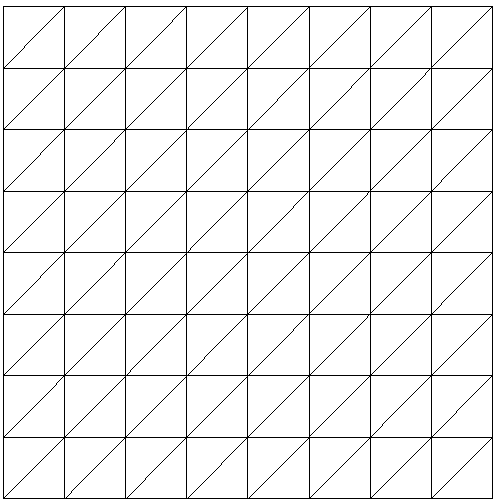
\includegraphics[width=.25\textwidth]{figures/grid1.png} \qquad  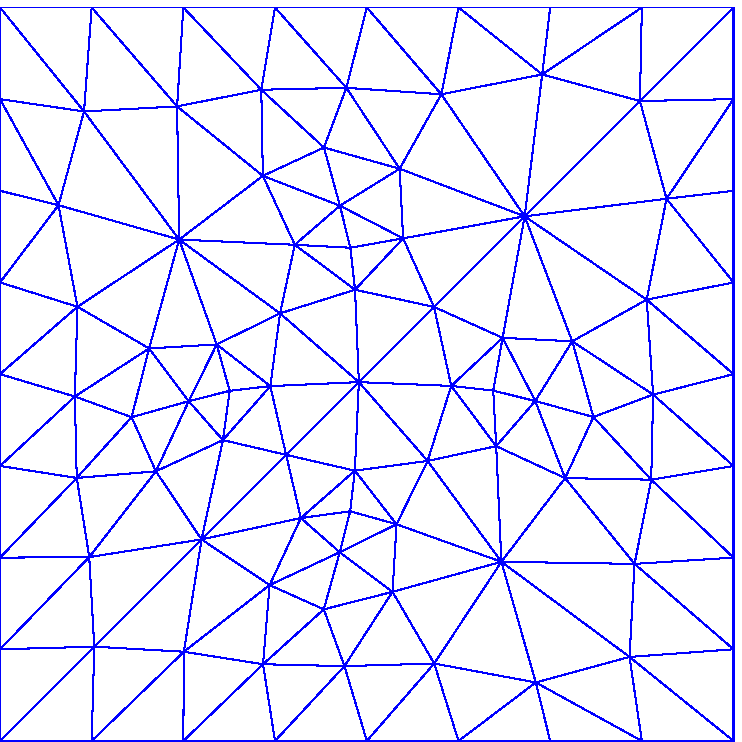
\includegraphics[width=.25\textwidth]{figures/u00.pdf}  \qquad 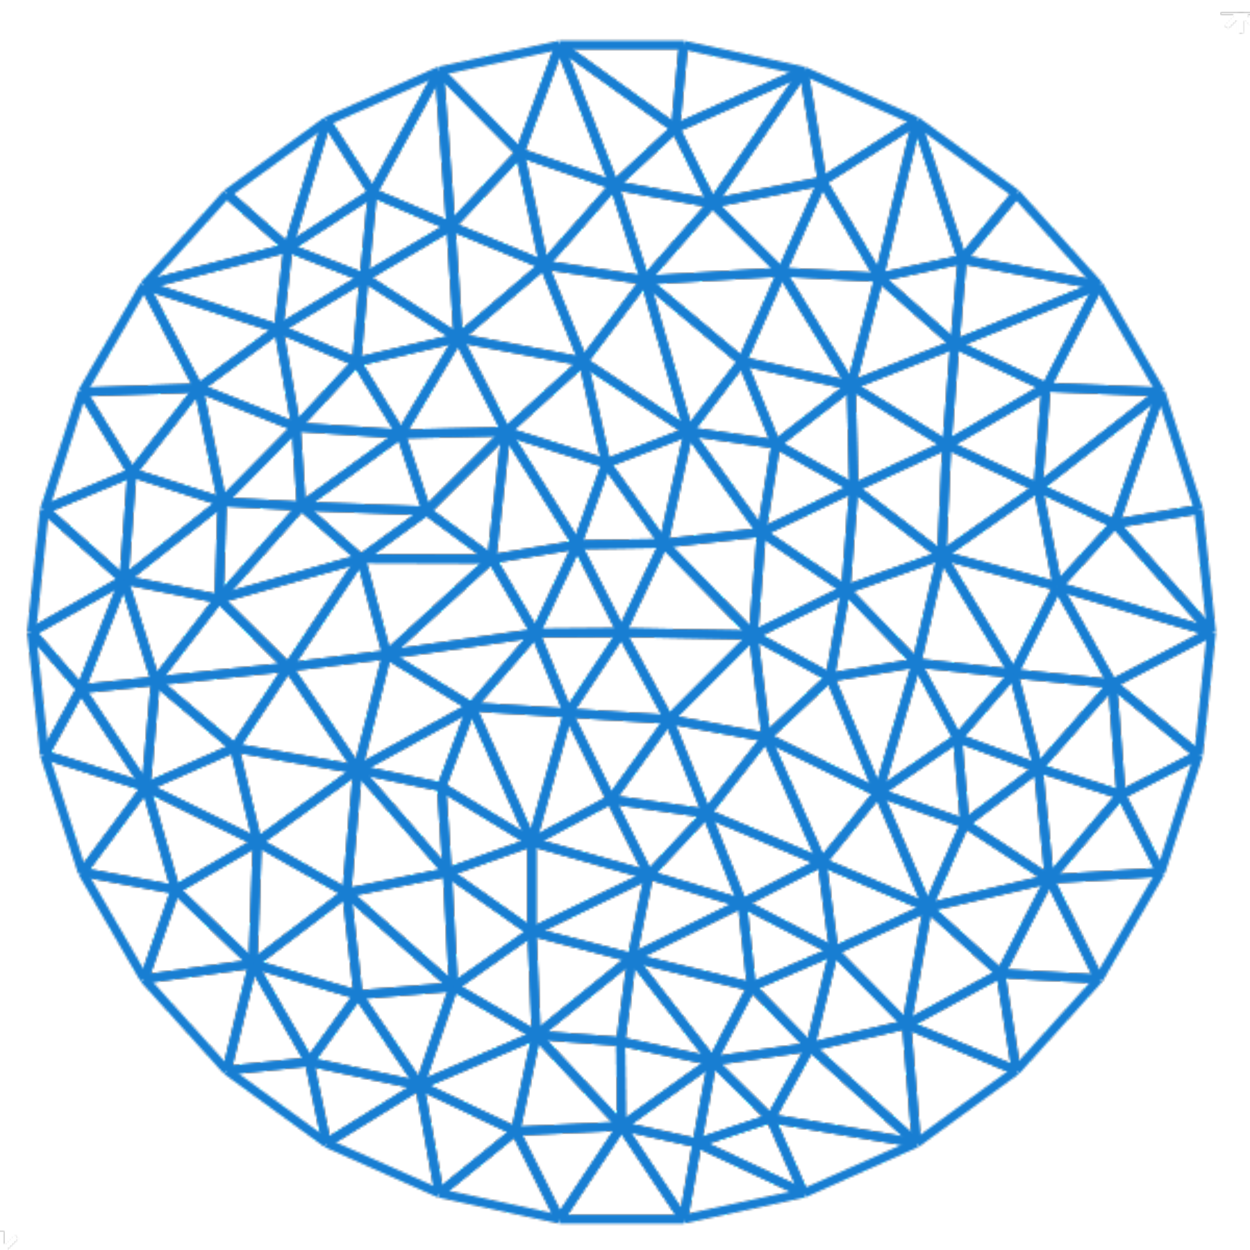
\includegraphics[width=.25\textwidth]{figures/2ddiskpartition.pdf}  
\end{center}
\caption{2D grids}
\label{2duniform}
\end{figure}

Denote 
$$
h_\tau=\mbox{\rm diam} (\tau)\quad  \hbox{(diameter of the smallest sphere containing $\overline{\tau}$)},
$$
and 
$$
 h=\max_{\tau\in\mathcal T_h} h_\tau;\quad
\underline{h}=\min_{\tau\in\mathcal T_h} h_\tau.
$$
A set of triangulations $\mathscr T$ is called {\em shape regular} if
there exists a constant $c_0$ such that
\begin{equation}\label{shape} \max _{\tau \in \mathcal T_h} \frac{h_{\tau}^d}{|\tau|}\leq c_0, \quad \forall \, \mathcal T_h\in
\mathscr T,
\end{equation} 
where $|\tau|$ is the measure of $\tau$ in $\mbb R^d$. This assumption can also be represented as
\begin{equation}\Label{A3.1}
\max_{\tau\in\ct_h}\frac{h_\tau}{\rho_\tau}\le\sigma_1,\quad \forall \, \mathcal T_h\in
\mathscr T,
\end{equation}
where $\rho_\tau$\index{$\rho_\tau$} denotes the radius of the ball
inscribed in $\tau$. In two dimensions, it is equivalent
to the minimal angle of each triange is bounded below uniformly
in the shape regular class. 
%We shall define $h_{\tau} = |\tau|^{1/n}$
%for any $\tau \in \mathcal T_h\in \mathscr T$. By (\ref{shape}),
%$h_{\tau}\eqsim {\rm diam}(\tau)$ represents the size of an element
%$\tau \in \mathcal T_h$ for a shape regular triangulation $\mathcal T_h\in
%\mathscr T$.

In addition to (\ref{shape}), if
\begin{equation}\Label{A3.2}
  \frac{\max _{\tau \in \mathcal T_h}|\tau|}{\min _{\tau \in \mathcal T_h}|\tau|} \leq \rho,\quad \forall \, \mathcal T_h\in \mathscr T,
\end{equation}
$\mathscr T$ is called {\em quasi-uniform}. For quasi-uniform grids,
$h=\max _{\tau \in \mathcal T_h} h_{\tau}$, the mesh size of
$\mathcal T_h$, is used to measure the approximation rate. 
%In the FEM literature, we often write as $\mathcal T_h$.

%The triangulation $\thset$ is said to be quasi-uniform
%\index{triangulation, quasi-uniform} if it satisfies \rf{A3.1} and
%the following
%\begin{eqhttps://gmu.zoom.us/j/97581839555?pwd=ZjlZeFE3Q0JkekdOcGpBZEZxdFJwQT09uation}\Label{A3.2}
%h\le\sigma_3 \underline {h}.
%\end{equation}

The assumption \rf{A3.1} is a local assumption, as is meant by above
definition, for $d=2$ for example, it assures that each triangle will
not degenerate into a segment in the limiting case.  
%A triangulation satisfying this assumption is often called to be {\it shape regular}.

On the other hand, the assumption \rf{A3.2} is a global assumption,
which says that the smallest mesh size is not too small compared with
the largest mesh size of the same triangulation.  By the definition, in
a quasi-uniform triangulation, all the elements are about the same size
asymptotically.

Let $ x_{i}=(x^1_{i}, \cdots, x^d_{i})^t, i=1,\cdots, d+1$ be $d+1$ points in $\mbb R^d$ which do not all lie in one hyper-plane. 
The {\it convex hull} of the $d+1$ points $ x_1, \cdots,  x_{d+1}$ (See Figure \ref{fig:barycentricCoor})
\begin{equation}
\tau :=\{ x=\sum _{i=1}^{d+1}\lambda _i x_i \, | \, 0\leq \lambda_i\leq 1, i=1:d+1, \sum _{i=1}^{d+1}\lambda _i=1 \}
\end{equation}
is defined as a {\em geometric $d$-simplex} generated (or spanned) by
the vertices $ x_1, \cdots,  x_{d+1}$. For example, a triangle
is a $2$-simplex and a tetrahedron is a $3$-simplex. For an integer
$0\leq m \leq d-1$, an $m$-dimensional face of $\tau$ is any
$m$-simplex generated by $m+1$ of the vertices of
$\tau$. Zero-dimenisonal faces are vertices and one-dimensional faces
are called edges of $\tau$. The $(d-1)$-face opposite to the vertex
$ x_i$ will be denoted by $F_i$.
\begin{figure}[hpt]
%\subfigure[1d simplex]{
%\begin{minipage}[t]{0.33\linewidth}
\centering
\includegraphics*[width=2.5cm]{figures/barycentricCoor1D.pdf}
%\end{minipage}}%%
%\subfigure[2d simplex]{
%\begin{minipage}[t]{0.33\linewidth}
%\centering
\includegraphics*[width=3cm]{figures/barycentricCoor2D.pdf}
%\end{minipage}}%%
%\subfigure[3d simplex]
%{\begin{minipage}[t]{0.33\linewidth}
%\centering
\includegraphics*[width=3.1cm]{figures/barycentricCoor3D.pdf}
%\end{minipage}}
\caption{Geometric explanation of barycentric coordinates}
\label{fig:barycentricCoor}
\end{figure}
%\paragraph{Barycentric coordinates}
On the other hand, for any $ x\in \tau$, there exist unique numbers $\lambda _1,\cdots, \lambda _{d+1}$ satisfying $\displaystyle 0\leq \lambda_i\leq 1, i=1:d+1, \sum _{i=1}^{d+1}\lambda _i=1$ such that $\displaystyle x=\sum _{i=1}^{d+1}\lambda _i x_i$, thus we can denote $\lambda _1,\cdots, \lambda _{d+1}$ as $\lambda _1( x),\cdots, \lambda _{d+1}( x)$. In fact,  the numbers $\lambda _1( x),\cdots, \lambda _{d+1}( x)$ are
called {\em barycentric coordinates} of $ x$ with respect to the
$d+1$ points $ x_1, \cdots,  x_{d+1}$. There is a simple
geometric meaning of the barycentric coordinates. Given a $ x\in
\tau$, let $\tau _i( x)$ be the simplex with vertices $ x_i$
replaced by $ x$. Then it can be easily shown that
\begin{equation}\label{eq:lambdasolution}
\lambda _i( x) = |\tau _i( x)|/|\tau|,
\end{equation}
where $|\cdot|$ is the Lebesgure measure in $\mbb R^d$, namely area in
two dimensions and volume in three dimensions. Note that $\lambda
_i( x)$ is affine function of $ x$ and vanishes on the face
$F_i$. We list the four basic properties of barycentric coordinate below:
\begin{enumerate}
\item $0\leq \lambda_i( x)\leq 1$;
\item $\displaystyle\sum_{i=1}^{d+1} \lambda_i( x)=1$;
\item $\lambda_i( x)\in P_1(\tau)$, where $P_1(\tau)$ denotes the space of polynomials of degree $1$
(linear) on $\tau\in \mathcal T_h$;
\item $\lambda_i( x_j)=\delta_{ij}=\begin{cases}
1, \quad &\text{if}  \quad  i=j\\
0, \quad &\text{if} \quad i\neq j
\end{cases}.$
\end{enumerate}

\subsection{Continuous linear finite element spaces}\label{linearFE}
A conforming linear finite element function in a domain $\Omega\subset
\mathbb R^d$ is a continuous function that is piecewise linear
function with respect to a grid or mesh consisting of a union of simplices.

Given a shape regular triangulation $\mathcal T_h$ of $\Omega$, we define the 
continuous linear finite element space as 
\begin{equation}\label{LinFE}
V_h:=\{v\,|\, v\in C(\overline \Omega), \,\hbox{ and }\, v|_{\tau}\in
P_1(\tau), \forall \tau \in \mathcal T_h\},
\end{equation}
where $P_1(\tau)$ denotes the space of polynomials of degree $1$
(linear) on $\tau\in \mathcal T_h$. Whenever we need to deal with boundary
conditions, we further define $V_{h,0}=V_h\cap H_0^1(\Omega)$.

We note here that the global continuity is also necessary in the
definition of $V_h$ in the sense that if $u$ has a square interable
gradient, that is $u\in H^1(\Omega)$, and $u$ is piecewise smooth,
then $u$ is continuous. 

We always use $n_h$ to denote the dimension of finite element
spaces. For $V_h$, $n_h$ is the number of vertices of the
triangulation $\mathcal T_h$ and for $V_{h,0}$, $n_h$ is the number of
interior vertices. 

\paragraph{Nodal basis functions and dual basis}
For linear finite element spaces, we have the so
called \emph{a standard nodal basis functions} $\{\varphi
_i,i=1,\cdots n_h\}$ such that $\varphi_i$ is piecewise linear (with
respect to the triangulation) and $\varphi_i(x_j)=\delta_{i,j}$.  Note
that $\varphi _i|_\tau$ is the corresponding barycentrical coordinates
of $x_i$. See Figure \ref{fig:nodalbasis} for an illustration in 2D.
\begin{figure}[hpt]
%\subfigure[1d basis function]{
%\begin{minipage}[t]{0.49\linewidth}
\centering
\includegraphics*[height=4.5cm,width=7cm]{6DL/figures/Dualbasis}
%\end{minipage}}
\caption{Dual basis functions of $V_h$ in 1D for $n_h=5$.}
\label{fig:dualbasis}
\end{figure}
Let $(\varphi_i^*)_{i=1}^{n_h}$ be the dual basis of $(\varphi_i)_{i=1}^{n_h}$, namely
\begin{equation}
  \label{eq:1}
(\varphi_i^*, \varphi_j) =\delta_{i, j}, \quad i, j=1,\ldots, n_h.    
\end{equation}
We notice that all the nodal basis functions $\{\varphi_i\}$ are locally
supported, but their dual basis functions $\{\varphi_i^*\}$ are in general
not locally supported (see Figure \ref{fig:dualbasis}).  The nodal basis functions $\{\varphi_i\}$ are
easily constructed in terms of barycentric coordinate functions.  The
dual basis $\{\varphi_i^*\}$ are only interesting for theoretical
consideration and it is not necessary to know the actual constructions
of these functions.

%
\begin{figure}[hpt]
%\subfigure[1d basis function]{
%\begin{minipage}[t]{0.49\linewidth}
\centering
\includegraphics*[height=4.5cm,width=7cm]{figures/basisfunction}
%\end{minipage}}%%
%\subfigure[2d basis function]{
%\begin{minipage}[t]{0.49\linewidth}
%\centering
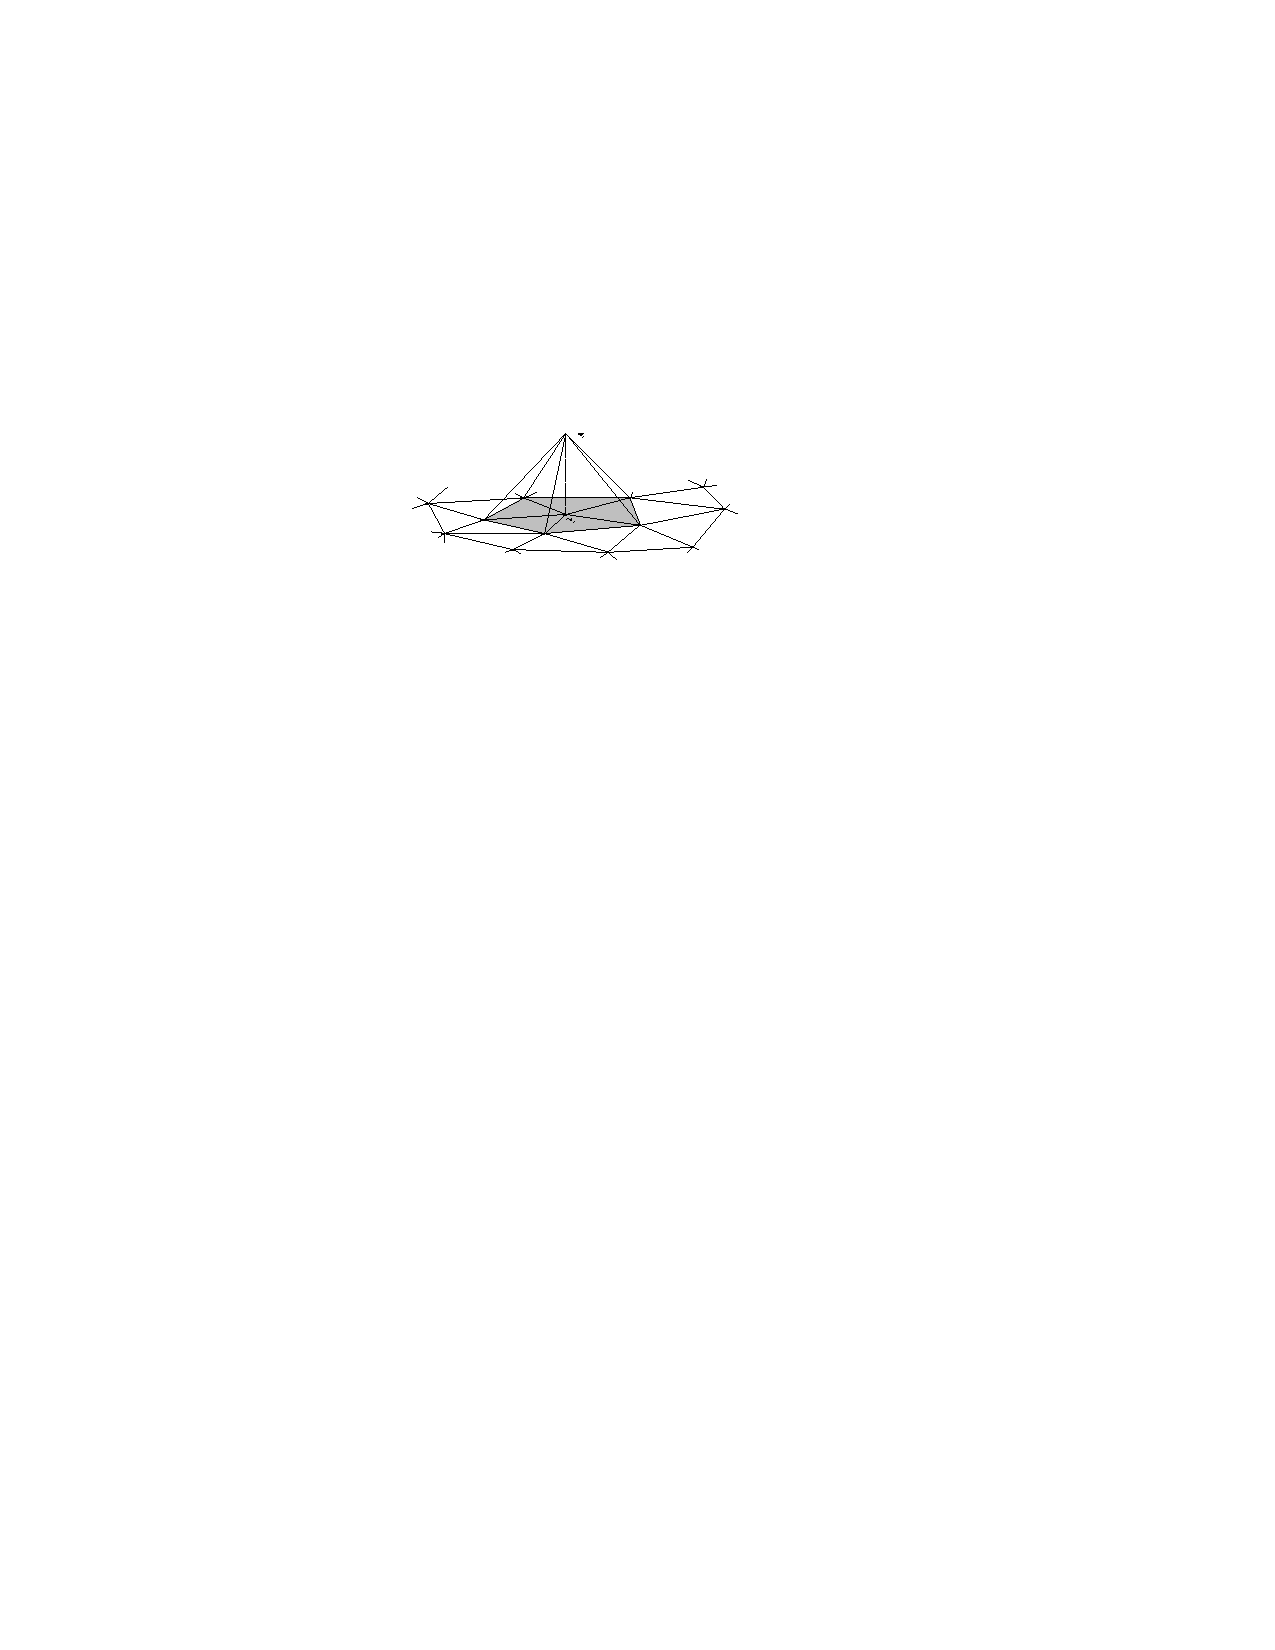
\includegraphics[height=5cm,width=7cm]{figures/nodalbasis.pdf}
%\end{minipage}}
\caption{Nodal basis functions in 1d and 2d}
\label{fig:nodalbasis}
\end{figure}
Since $\{\varphi_i,i=1,\cdots n_h\}$ is a basis of $V_h$, therefore for any $v_h\in V_h$, we have the representation
$$
v_h(x)=\sum_{i=1}^{n_h}v_h(x_i)\varphi_i(x). 
$$

Let us see how our construction of continuous linear finite space and the nodal basis looks like  in one spatial dimension. 
Associated with the mesh
$$
\mathcal T_h=\{0=x_0<x_1<\ldots<x_{n_h}<x_{n_h+1}=1\},
$$
by the definition given in \eqref{LinFE} and the definition  $V_{h,0}=V_{h}\cap H_0^1(\Omega)$, we have
\[
\begin{array}{ll}
V_{h,0}=\{v:~\mbox{$v$ is continuous and piecewise linear}~ \mbox{w.~r.~t. $\mathcal T_h$, } v(0)=v(1)=0\}.
\end{array}
\]
A plot of a typical element of $V_{h,0}$ is shown in Fig.~\ref{fig:1dtypical}.

It is easily calculated (as we already mentioned), that the dimension
of $V_{h,0}$ is equal to the number of internal vertices, and the nodal
basis functions spanning $V_{h,0}$ (for $i=1,2,\cdots,n_h$) are (see also
Fig.~\ref{fig:nodalbasis}):
\begin{equation}\label{1dbasis:function}
\varphi_i(x)=\left\{\begin{array}{cl}
\displaystyle \frac{x-x_{i-1}}{h}, & x\in[x_{i-1},x_i];\\
\displaystyle \frac{x_{i+1}-x}{h}, & x\in[x_{i},x_{i+1}];\\
0 &\mbox{elsewhere}.
\end{array}\right.
\end{equation}

\begin{figure}[hpt]
\centering
\includegraphics*[width=2in]{figures/femfunction1.pdf}
\caption{Plot of a typical element from $V_{h,0}$.} 
\label{fig:1dtypical}
\end{figure}



%%%%%%%%%%%%%%%%%%%%END from grid.tex%%%%%%%%%%%%%%%%%%%%%%%%%%%%%%%

%%%%%%%%%%%%%%%%%%%%END from grid.tex%%%%%%%%%%%%%%%%%%%%%%%%%%%%%%%

%%%%%%%%%%%%%%%%%%%%END from grid.tex%%%%%%%%%%%%%%%%%%%%%%%%%%%%%%%

\paragraph{Nodal value interpolant}
\Label{sc-seio}

For any continuous function $u$, we define its linear finite element
interpolation, $(I_h u)(x)\in V_{h,0}$,  as follows:
\begin{equation}
  \label{u-interp}
(I_h u)(x)= \sum_{i=1}^{n_h}u(x_i)\varphi_i(x).
\end{equation}
Usually, we also denote $(I_h u)(x)$ as $u_I(x)$. Using interpolation, we can obtain the following approximation property of 
linear finite element space. 
%For any $v\in\Shz$, we can obviously write
%$$
%        v(x)=\sum_{i=1}^{n_h}v(x_i)\phi_i(x).
%$$
%The nodal value interpolation\index{interpolation} operator $I_h: C(\bar\Om)\mapsto V_h$ is defined as follows \index{$I_h$}
%$$
%        (I_h u)(x_i)=u(x_i),\qall x_i\in {\cal N}_h,
%$$
%where ${\cal N}_h$ is the set of the vertexes for the partition $\mathcal T_h$. 
\begin{figure}[hpt]
\begin{center}
\includegraphics*[height=2.5in, width=3in]{figures/fdsolutions.pdf}
\caption{Approximation of finite element space.} 
\label{Interpolation}
\end{center}
\end{figure}


\begin{theorem}\label{interp00}
Assume that $\mathcal T_h$ is quasi-uniform and $V_h$ is the linear finite element space associated with $\mathcal T_h$, then
\begin{equation}
\label{error0}
\inf_{v_h\in V_h} \|v-v_h\|+h |v-v_h|_{1}\lc h^2 |v|_2
        \qall v\in H^2(\Om).
\end{equation}
 \end{theorem}
 \begin{proof}  
Let us first prove Theorem \ref{interp00} for $d=1, 2, 3$.
This proof presented here follows from Xu~\cite{xu1982estimate} (see also Xu~\cite{xu2013estimate}).
Let $x=(x^1,\ldots, x^d)$ and $a_i=(a^1_{i}, \ldots, a^d_{i})$. Introducing
the auxiliary functions
$$
g_i(t)=v(a_i(t)),\mbox{  with  }  a_i(t)=a_i+t(x-a_i),
$$
we have
$$
g_i'(t)=(\nabla v)(a_i(t))\cdot (x-a_i)
=\sum_{l=1}^d(\partial_lv)(a_i(t))(x^l-a_i^l)
$$
and
\begin{equation}\label{gpp}
g_i''(t)=\sum_{k,l=1}^d\partial^2_{kl}v)(a_i(t))(x^k-a_i^k)(x^l-a_i^l).
\end{equation}
Note Taylor expansion
$$
        g_i(0)=g_i(1)-g_i'(1)+\int_0^1tg''_i(t)dt,
$$
namely
\begin{equation}\label{Taylor_vi}
v(a_i)=v(x)-(\nabla v)(x)\cdot (x-a_i)+\int_0^1tg''_i(t)dt,
\end{equation}
and note that
$$
(I_hv)(x)=\sum_{i=1}^{d+1}v(a_i)\lambda_i(x), \quad \sum_{i=1}^{d+1}\lambda_i(x)=1,
$$
and
$$
\sum_{i=1}^{d+1}(x-a_i)\lambda_i(x)=0.
$$
It follows that
\begin{equation}\label{Ihvv}
(I_hv-v)(x)=\sum_{i=1}^{d+1}\lambda_i(x)\int_0^1tg''_i(t)dt.
\end{equation}
Using \rf{gpp} and the trivial fact that $|x^l-a_i^l|\le h$,
we obtain
\begin{eqnarray*}
\|g''_i(t)\|_{L^2(\tau)}\le h^2
\sum_{k,l=1}^d\|(\partial^2_{kl}v)(a_i(t))\|_{L^2(\tau_i^t)}
\le h^2t^{-d/2}\sum_{k,l=1}^d\|\partial^2_{kl}v\|_{L^2(\tau)},
\end{eqnarray*}
where we have used the following change of variable
$$
y=a_i+t(x-a_i): \tau\mapsto \tau_i^t\subset\tau \mbox{ with } dy=t^ddx.
$$
Now taking the $L^2(\tau)$ norm on both hand of sides of
\rf{Ihvv}, we get
\begin{eqnarray*}
\|I_hv-v\|_{L^2(\tau)}
&\le& h^2\sum_{i=1}^{d+1}\max_{x\in\tau}|\lambda_i(x)|
\int_0^1t\|g''_i(t)\|_{L^2(\tau)}\;dt\\
&\le& (d+1)\int_0^1t^{-d/2}dt\;h^2\;
\sum_{k,l=1}^d\|\partial^2_{kl}v\|_{L^2(\tau)}\\
&\le&\frac{2(d+1)}{4-d}h^2
\sum_{k,l=1}^d\|\partial^2_{kl}v\|_{L^2(\tau)}\\
&\le&\frac{4d(d+1)}{4-d}h^2|v|_{H^2(\tau)}.
\end{eqnarray*}
Now we prove the $H^1$ error estimate. Notice that
$$
[\partial_{j}( I_{h} v - v)](x) = \sum_{i} (\partial_{j} \lambda_{i} )(x) \int_{0}^{1} t g''_{i}(t) dt + \sum_{i} \lambda_{i}(x) \partial_{j} \int_{0}^{1} t g''_{i}(t) dt.
$$ 
By \rf{Taylor_vi},
$$
\int_0^1tg''_i(t)dt = v(a_i) - v(x) + (\nabla v)(x)\cdot (x-a_i)
$$
therefore,
\begin{eqnarray*}
\lefteqn{\partial_{j} \int_0^1tg''_i(t)dt} \\
& = & - \partial_{j} v + (\nabla \partial_{j} v )(x) (x - a_{i}) + \nabla v \cdot e_{j} 
\hcomment{$e_{j}$ is the $j$-th standard basis}  \\
& = & (\nabla \partial_{j} v )(x) (x - a_{i}).
\end{eqnarray*}
Noting that $\sum_{i} \lambda_{i}( \nabla \partial_{j} v )(x) (x - a_{i}) = 0$, we have
$$
[\partial_{j}( I_{h} v - v)](x) = \sum_{i} (\partial_{j} \lambda_{i} )(x) \int_{0}^{1} t g''_{i}(t) dt.
$$
Then the estimate for $|\nabla(I_hv-v)|_{L^2(\tau)}$
follows by a similar argument and the following obvious
estimate
$$
|(\nabla\lambda_i)(x)|\lc\frac{1}{h}.
$$
 
On the proof of Theorem \ref{interp0} for $d\ge 4$, the above proof does not
apply for $d \ge 4$. This is because when $d \ge 4$, the embedding
relation between $H^{2}(\Om) \hookrightarrow C(\bar{\Om})$ is no longer true.  Only
continuous functions can have interpolations. In this case, one approach is to use the 
so-called Scott-Zhang interpolation \cite{scott1990finite}, the
details can be found in \cite{Xu.J2015a}.
\end{proof}
As a result of Theorem \ref{interp00}, we have
\begin{theorem}\label{interp0}
Let $V_N$ be linear finite element space on a quasi-uniform
triangulation consisting of $N$ element.  Then 
\begin{equation}
\label{error0N}
\inf_{v_h\in V_N} \|v-v_h\|+N^{-{1\over d}} |v-v_h|_{1}\lc N^{-{2\over d}} |v|_2
        \qall v\in H^2(\Om).
\end{equation}
\end{theorem}





\chapter{Deep Neural Network Functions}
\section{Motivation: from finite element to neural network}\label{FE2NN}
In this section, we will introduce the so-called shallow neural network 
(deep neural network with one hidden layer) from the viewpoint of finite element method.

Let us recall the linear finite element functions on the unit interval $\bar{\Omega}=[0,1]$ in Section \ref{linearFE}. 
Consider a set of equidistant girds $\mathcal T_\ell$ of level $\ell$ and mesh length $h_\ell = 2^{-\ell}$. The grid points $x_{\ell,i}$ are given by
\begin{equation}
x_{\ell,i}:=ih_\ell,\quad 0\le i\le 2^\ell.
\end{equation} 
For $\ell=1$, we denote the special hat function by $\varphi(x)$ and any nodal basis function in \eqref{1dbasis:function} on grid $\mathcal T_\ell$ by $\varphi_{\ell,i} $ as below
\begin{equation}\label{def_g}
\varphi(x) = 
\begin{cases}
2x \quad &x\in [0,\frac{1}{2}] \\
2(1-x) \quad &x\in [\frac{1}{2}, 1] \\
0, \quad &\text{others} 
\end{cases},\qquad
\varphi_{\ell,i} = \varphi(\frac{x - x_{\ell,i-1}}{2h_\ell}) = \varphi(w_\ell x + b_{\ell,i}).
\end{equation} 
That is to say, any $\varphi_{\ell,i}(x)$ can be obtained from $\varphi(x)$ by scaling 
(dilation) and translation with 
\begin{equation}\label{key}
w_\ell = 2^{\ell-1}, \quad b_{\ell,i} = \frac{-(i-1)}{2},
\end{equation}
in $\varphi_{\ell,i} = \varphi(w_\ell x + b_{\ell,i})$. 
\begin{figure}[H]
\centering
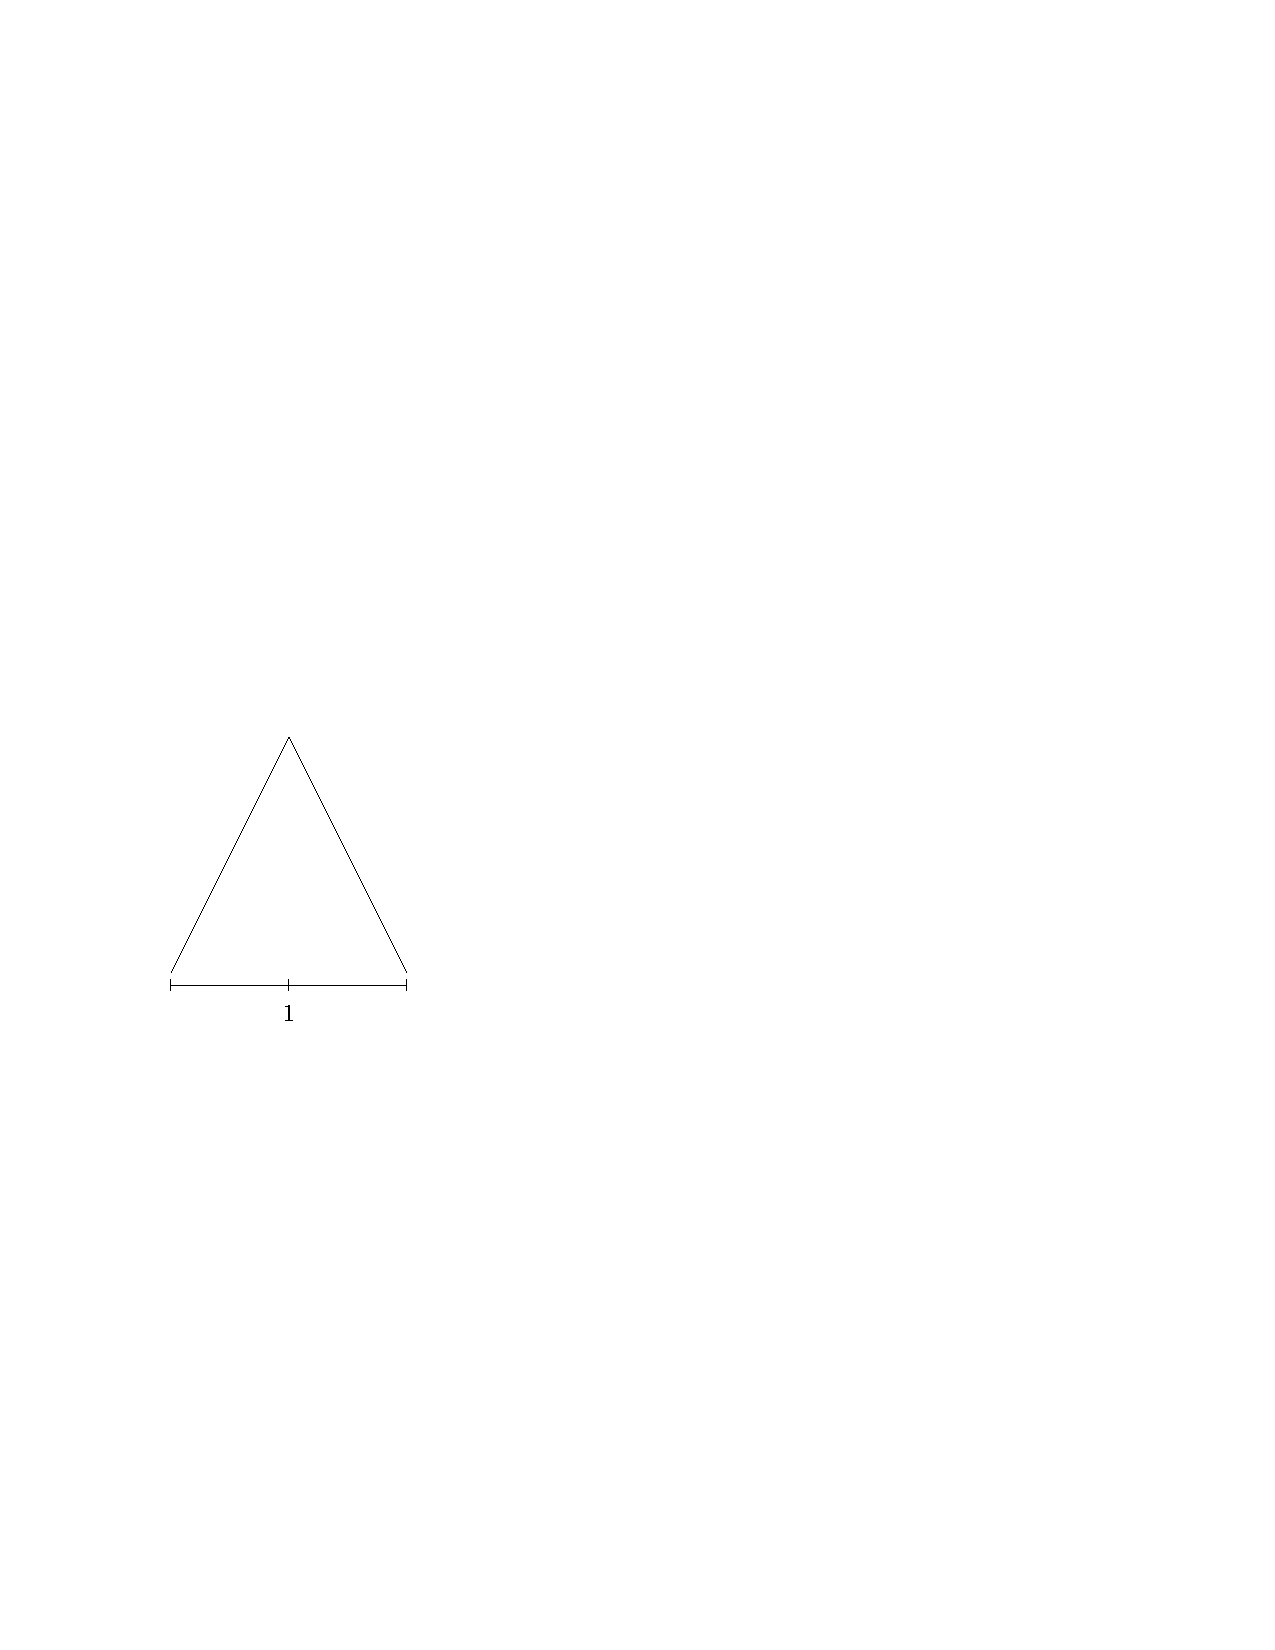
\includegraphics[width=4cm]{1dbasis1.pdf}\qquad
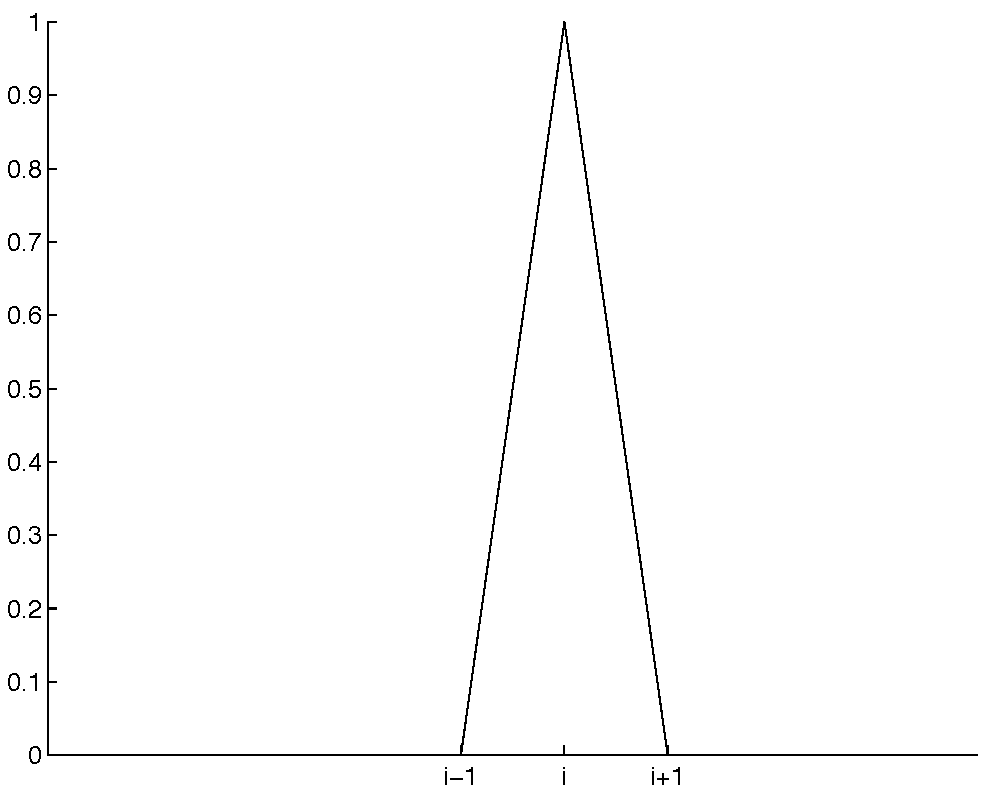
\includegraphics[width=5cm]{basisfunction.pdf}
\caption{Diagram of $\varphi(x)$ (left) and $\varphi_{\ell,i}(x)$ (right).}
\end{figure} 


Let us recall the finite element interpolation in Section \ref{linearFE} as
\begin{equation}\label{key}
u(x) \approx u_\ell(x) := \sum_{ 0\le i \le 2^\ell} u(x_{\ell,i}) \varphi_{\ell,i}(x),
\end{equation}
for any smooth function $u(x)$ on $(0,1)$. The above interpolation will converge as $\ell \to \infty$, which shows that
\begin{equation}\label{key}
{\rm span} \left\{  \varphi(w_\ell x + b_{\ell,i}) \right\} \quad \text{is dense in} \quad H^1(0,1).
\end{equation}
Thus, we may have the next concise relation:
\begin{equation}\label{key}
\begin{split}
\text{FE space} =  &{\rm span} \left\{  \varphi(w_\ell x + b_{\ell,i}) ~|~ 0\le i \le 2^\ell, \ell = 1, 2, \cdots \right\} 
\\
\subset  &{\rm span} \left\{  \varphi(w x + b) ~|~  w, b \in \mathbb{R} \right\}.
\end{split}
\end{equation}
In other words, the finite element space can be understood as the linear combination of $\varphi(w x + b)$ with certain special choice of $w$ and $b$. 

Here, we need to point out that this ${\rm span} \left\{  \varphi(w x + b) ~|~  w, b \in \mathbb{R} \right\}$ is exact the deep neural networks with one hidden layer (shallow neural networks) with activation function $\varphi(x)$. More precisely, 
\begin{equation}\label{key}
f \in {\rm span} \left\{  \varphi(w x + b) ~|~  w, b \in \mathbb{R} \right\},
\end{equation}
means there exist positive integer $N$ and $w_j, b_j \in \mathbb{R}$ such that 
\begin{equation}\label{key}
f = \sum_{j=1}^N a_j \varphi(w_j x + b_j),
\end{equation}
which is also called one hidden neural network function with $N$ neurons.

\begin{remark}
	\begin{enumerate}
		\item By making $w_\ell$ and $b_{\ell,i}$ in \eqref{def_g} arbitrary, we get a much larger class of 
		function which is exact a special neural network with activation function $\varphi(x)$.
		\item Generalizations: 
		\begin{enumerate}
			\item activation function $\varphi$ can be different, such as ${\rm ReLU}(x) = \max\{0,x\}$.
			\item There is a natural extension for high dimension $d$ as
			\begin{equation}\label{key}
			\left\{  \varphi(w\cdot x + b) \right \},
			\end{equation}
			where $w\in \mathbb{R}^d$, $b\in \mathbb{R}$ and $\displaystyle w\cdot x = \sum_{i=1}^d w_i x_i$.
			This is called ``deep'' neural network with one hidden layer.
		\end{enumerate}
	\end{enumerate}
\end{remark}


%\input{3FEM/2dFEM}

\section{Why we need deep neural networks via composition}\label{whydeep}
\subsection{FEM ans ${\rm DNN}_1$ in 1D}
Thanks to following connection between $\varphi(x)$ in \eqref{def_g} and ${\rm ReLU}(x) = \max(0,x )=x_+$
\begin{equation}\label{key}
\varphi(x) = 2{\rm ReLU}(x) - 4{\rm ReLu}({x-\frac{1}{2}}) + 2{\rm ReLU}(x-1),
\end{equation}
it suffices to show that each basis
function $\varphi_{\ell,i}$ can be represented by a ReLU DNN. 
We first note that  the basis
function $\varphi_{\ell,i}$ has the support in $[x_{\ell,i-1},
x_{\ell,i+1} ]$ can be easily written as
\begin{equation}
\label{1d-basisu}
\varphi_{\ell,i}(x) = \frac{1}{h_{\ell}}{\rm ReLU}(x-x_{\ell,i-1}) -\frac{2}{h_{\ell}}{\rm ReLU}(x-x_{\ell,i}) +\frac{1}{h_\ell}{\rm ReLU}(x-x_{\ell,i+1}).
\end{equation}
More generally, consider a general  grid with vertex $\{x_i\}$, which is not necessarily uniform. The basis function $\varphi_i$ of the linear element with support $[x_{i-1},
x_{i+1} ]$ can be easily written as
\begin{equation}
\label{1d-basis}
\varphi_i(x) = \frac{1}{h_{i-1}}{\rm ReLU}(x-x_{i-1}) -(\frac{1}{h_{i-1}}+\frac{1}{h_i}){\rm ReLU}(x-x_i) +\frac{1}{h_i}{\rm ReLU}(x-x_{i+1}),
\end{equation}
where $h_i = x_{i+1} - x_i$.

Thus is to say, we have the next theorem.
\begin{theorem}\label{thm:1dLFEMDNN}
	For $d=1$, and  $\Omega\subset \mathbb R^d$ is 
	a bounded interval, then ${\rm DNN}_1$ can be used to cover all linear finite element 
	function in on $\Omega$.
\end{theorem}
\subsection{Linear finite element cannot be recovered by ${\rm DNN}_1$ for $d\ge2$}
In view of  Theorem~\ref{thm:1dLFEMDNN} and the fact that ${\rm{DNN}_J}
\subseteq {\rm{DNN}_{J+1}} $, it is natural to ask that how many
layers are needed at least to recover all linear finite element
functions in $\mathbb{R}^d$ for $d\ge2$.  In this section, we will show that 
\begin{equation}\label{key}
J_d \ge 2, \quad \text{if} \quad d\ge 2,
\end{equation}
where $J_d$ is the minimal $J$ such that all linear finite element
functions in $\mathbb R^d$ can be recovered by ${\rm DNN}_J$.

In particular, we will show the following theorem~\cite{he2020relu}.
\begin{theorem}\label{lowerbound}
	If $\Omega\subset \mathbb R^d$ is either 
	a bounded domain or $\Omega=\mathbb{R}^d$,  
	${\rm DNN}_1$ can not be used to recover all linear finite element
	functions on $\Omega$. 
\end{theorem}
\begin{proof}
	We prove it by contradiction. Let us assume that for any continuous
	piecewise linear function $f: \Omega \to \mathbb{R} $, we can find
	finite $N \in \mathbb{N}$, $w_i \in \mathbb{R}^{1,d}$ as row vector
	and $\alpha_i, b_i, \beta \in \mathbb{R}$ such that
	$$
	f =  \sum_{i=1}^N \alpha_i {\rm ReLU}(w_i\cdot  x +b_i) + \beta,
	$$
	with $f_i = \alpha_i {\rm ReLU}(w_i\cdot  x +b_i)$, $\alpha_i \neq 0$ and $w_i
	\neq 0$.  Consider the finite element functions, if this one hidden
	layer ReLU DNN can recover any basis function of FEM, then it can
	recover the finite element space.  Thus let us assume $f$ is a locally
	supported basis function for FEM.
	Furthermore, if $\Omega$ is a bounded domain, we assume that 
	\begin{equation}\label{distcondi}
	d({\rm supp}(f), \partial \Omega) > 0,
	\end{equation}with 
	$$
	d(A, B) = \inf_{x\in A, y\in B} \|x-y\|,
	$$ 
	as the distance of two closed sets. 
	
	A more important observation is that $\nabla f: \Omega \to
	\mathbb{R}^d$ is a piecewise constant vector function. The key
	point is to consider the discontinuous points for 
	$$g := \nabla
	f = \sum_{i=1}^N \nabla f_i.$$
	For more general case, we can define the set of discontinuous points of a function by
	$$
	D_{g} := \{x \in \Omega~|~ x ~ \text{is a discontinuous point of} ~ g\}.
	$$
	Because of the property that 
	\begin{equation}\label{eq:disfun}
	D_{f+g} \supseteq D_{f} \cup D_{g} \backslash (D_{f} \cap D_{g}),
	\end{equation}
	we have
	\begin{equation}\label{eq:dis_fn}
	D_{\sum_{i=1}^N g_i} \supseteq \bigcup_{i=1}^N D_{g_i} \backslash \bigcup_{i\neq j}\left( D_{g_i}\cap D_{g_j} \right).
	\end{equation}
	Note that
	\begin{equation}\label{eq:def_gi}
	g_i = \nabla f_i(x) =  \nabla \left( \alpha_i {\rm ReLU}(w_i\cdot   x +b_i)  \right) =\left(\alpha_iH(w_i \cdot  x +b_i)\right)w_i \in \mathbb{R}^d,
	\end{equation}
	for $i=1:N$ with $H$ be the Heaviside function defined as: 
	$$
	H(x) = \begin{cases}
	0 &\text{if} ~ x \le 0, \\
	1 &\text{if} ~ x > 0.
	\end{cases}
	$$ 
	This means that 
	\begin{equation}\label{eq: D_gi}
	D_{g_i} = \{ x ~|~ w_i\cdot   x + b_i = 0\}
	\end{equation}
	is a $d-1$ dimensional affine space in $\mathbb{R}^d$.  
	
	
	Without loss of generality, we can assume that 
	\begin{equation}\label{eq:assumD_gi}
	D_{g_i} \neq D_{g_j}.
	\end{equation}
	When the other case occurs, i.e. $D_{g_{\ell_1}} = D_{g_{\ell_2}} = \cdots= D_{g_{\ell_k}}$, by the definition of $g_i$ in \eqref{eq:def_gi} and $D_{g_i}$ in \eqref{eq: D_gi} , 
	this happens if and only if there is a row vector $(w, b)$ such that
	\begin{equation}\label{eq:Dfcondition}
	c_{\ell_i}\begin{pmatrix}
	w &
	b
	\end{pmatrix} =  
	\begin{pmatrix}
	w_{\ell_i} &
	b_{\ell_i}
	\end{pmatrix},
	\end{equation}
	with some $c_{\ell_i} \neq 0$ for $i = 1:k$.  We combine those $g_{\ell_i}$ as
	\begin{equation*}
	\begin{aligned}\label{mergeH}
	%	\begin{split}
	\tilde g_{\ell} &= \sum_{i=1}^k g_{\ell_i} = \sum_{i=1}^k \alpha_{\ell_i} H(w_{\ell_i} \cdot  x + b_{\ell_i}) w_{\ell_i}, \\
	&= \sum_{i=1}^k \left( c_{\ell_i}\alpha_{\ell_i} H\left(c_{\ell_i}(w\cdot   x + b)\right) \right) w, \\
	&=\begin{cases}
	\displaystyle \left(\sum_{i=1}^k  c_{\ell_i}\alpha_{\ell_i} H(c_{\ell_i}) \right) w  \quad &\text{if} \quad w x + b > 0,\\
	\displaystyle \left(\sum_{i=1}^k  c_{\ell_i}\alpha_{\ell_i} H(-c_{\ell_i}) \right) w  \quad &\text{if} \quad w x + b \le 0.\\
	\end{cases}
	%	\end{split}
	\end{aligned}
	\end{equation*}	
	Thus, if 
	$$
	\left(\sum_{i=1}^k  c_{\ell_i}\alpha_{\ell_i} H(c_{\ell_i}) \right)  = \left(\sum_{i=1}^k  c_{\ell_i}\alpha_{\ell_i} H(-c_{\ell_i}) \right),
	$$
	$\tilde g_\ell$ is a constant vector function, that is to say $D_{\sum_{i=1}^k g_{\ell_i}} = D_{\tilde g_\ell} = \emptyset$. 
	Otherwise, $\tilde g_\ell$ is a piecewise constant vector function with the property that 
	$$
	D_{\sum_{i=1}^k g_{\ell_i}} = D_{\tilde g_\ell} = D_{g_{\ell_i}} = \{ x ~|~ w\cdot  x + b = 0\}.
	$$
	This means that we can use condition \eqref{eq:Dfcondition} as an equivalence relation and split $\{g_i\}_{i=1}^N$ into some groups, and we can combine those $g_{\ell_i}$ in each group as what we do above. After that, we have
	$$
	\sum_{i=1}^N g_i = \sum_{\ell=1}^{\tilde N} \tilde g_{\ell},
	$$
	with $D_{\tilde g_s} \neq D_{\tilde g_t}$.
	Finally, we can have that $D_{\tilde g_s} \cap D_{\tilde g_t}$ is an empty set or a $d-2$ dimensional affine space in $\mathbb{R}^d$.
	Since
	$\tilde N \le N$ is a finite number, 
	$$
	D := \bigcup_{i=1}^N D_{\tilde g_\ell} \backslash \bigcup_{s\neq t}\left( D_{\tilde g_s}\cap D_{\tilde g_t} \right)
	$$
	is an unbounded set. 
	\begin{itemize}
		\item If $\Omega = \mathbb{R}^d$,
		$$
		{\rm supp(f)} \supseteq D_{g} = D_{\sum_{i=1}^N g_i} = D_{ \sum_{\ell=1}^{\tilde N} \tilde g_{\ell}} \supseteq D,
		$$ is contradictory to the assumption that $f$ is locally supported.
		\item If $\Omega$ is a bounded domain, 
		$$
		d(D, \partial \Omega) = 
		\begin{cases}
		s > 0 \quad &\text{if}\quad  D_{\tilde g_i} \cap \Omega = \emptyset, \forall i\\
		0 \quad &\text{otherwise}.
		\end{cases}
		$$
		Note again that all $D_{\tilde g_i}$'s are $d-1$ dimensional affine spaces, while $D_{\tilde g_i} \cap D_{\tilde g_j}$ is either an empty set or a d-2 dimensional affine space. 
		If $d(D, \partial \Omega) > 0$, this implies that $\nabla f$ is continuous in $\Omega$, which contradicts the  assumption that $f$ is a basis function in FEM.
		If $d(D, \partial \Omega) = 0$, this contradicts the previous assumption in \eqref{distcondi}.
	\end{itemize}
	Hence ${\rm DNN}_1$ cannot recover any piecewise linear function in $\Omega$ for $d \ge 2$.
\end{proof}

Following the proof above, we have the following theorem~\cite{he2020relu}.
\begin{theorem}\label{linearindep}
	$\{{\rm ReLU}(w_i\cdot x+b_i)\}_{i=1}^m$ are linearly independent if $(w_i,
	b_i)$ and $(w_j, b_j)$ are linearly independent in
	$\mathbb{R}^{1\times (d+1)} $ for any $i \neq j$.
\end{theorem}






\section{Definition of deep neural networks (DNN)} 
In this section, we will give a brief introduction to a special
function class related to deep neural networks (DNN) used in machine
learning.  We then explore the relationship between DNN (with ReLU as
activation function) and linear finite element methods. 

Given $n, m\ge 1$, the first ingredient in defining a deep neural
network (DNN) is (vector) linear functions of the form
\begin{equation}\label{thetamap1}
\theta:\mathbb{R}^{n}\to\mathbb{R}^{m} ,
\end{equation}as $\theta(x)=Wx+b$ where
$W=(w_{ij})\in\mathbb{R}^{m\times n}$, $b\in\mathbb{R}^{m}$. 
The second main ingredient is a nonlinear activation function, usually
denoted as 
\begin{equation}\label{sigma}
\sigma: \mathbb{R} \to \mathbb{R}.
\end{equation} 
By applying the function to each component, we can extend this
naturally to 
$$
\sigma:\mathbb R^{n}\mapsto \mathbb R^{n}.
$$


\subsection{Definition of neurons}
\begin{enumerate}
	\item Primary variables $n_0=d$
	$$
	x^0=x=
	\begin{pmatrix}
	x_1\\
	x_2\\
	\vdots \\  
	x_{d}
	\end{pmatrix}
	$$
	\item $n_1$ hyperplanes $\theta^{0}(x^0) = W^0 x + b^0$ where $W^0: \mathbb{R}^{d} \mapsto \mathbb{R}^{n_1}$:
	$$
	W^0x+b^0=
	\begin{pmatrix}
	w^0_1x+b^0_1\\
	w^0_2x+b^0_2\\
	\vdots \\  
	w^0_{n_1}x+b^0_{n_1}
	\end{pmatrix}\quad \mbox{with }\quad W^0=
	\begin{pmatrix}
	w^0_1\\
	w^0_2\\
	\vdots \\  
	w^0_{n_1}
	\end{pmatrix},\quad b^0=
	\begin{pmatrix}
	b^0_1\\
	b^0_2\\
	\vdots \\  
	b^0_{n_1}
	\end{pmatrix}
	$$
	\item $n_1$-neurons:
	$$
	x^1=\sigma(W^0x+b^0)
	=\begin{pmatrix}
	\sigma(w^0_1x+b^0_1)\\
	\sigma(w^0_2x+b^0_2)\\
	\vdots \\  
	\sigma(w^0_{n_1}x+b^0_{n_1})
	\end{pmatrix}
	$$
%	\begin{center}
%	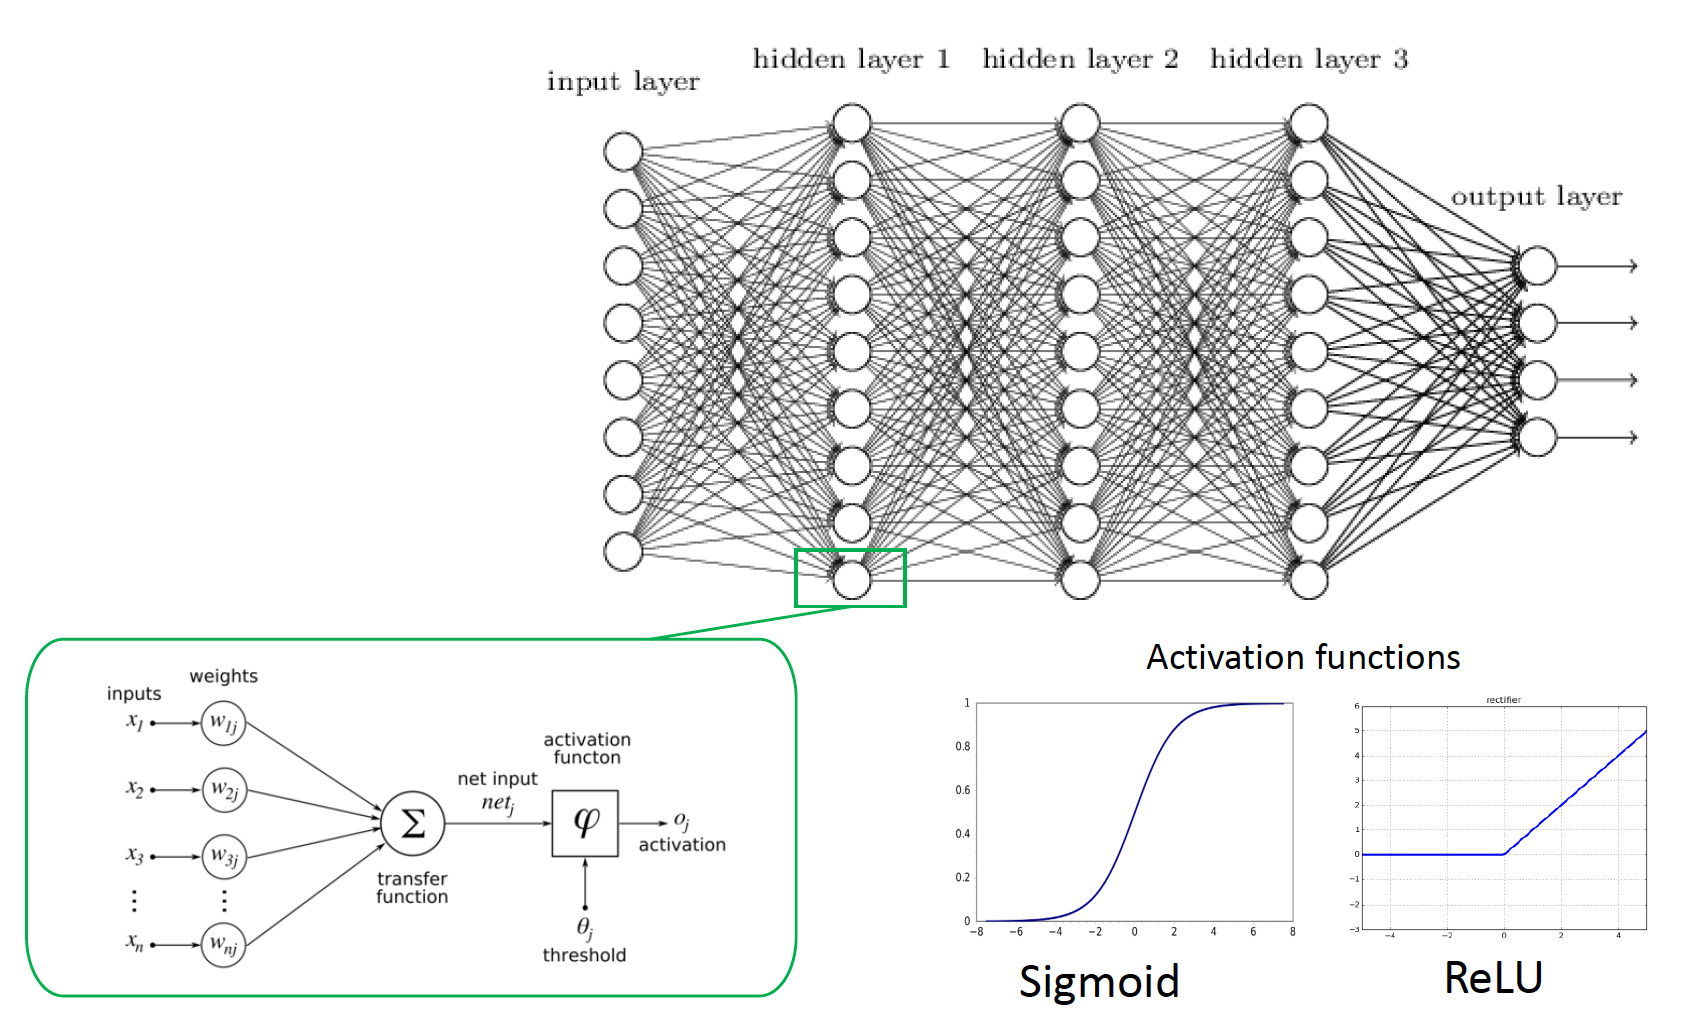
\includegraphics[height=.5\textwidth]{ANN}
%	\end{center}
	
	\item $n_2$-hyperplanes $\theta^{1}(x^1) = W^1 x + b^1$ where $W^1: \mathbb{R}^{n_1} \mapsto \mathbb{R}^{n_2}$:
	$$
	W^1x^1+b^1=
	\begin{pmatrix}
	w^1_1x^1+b^1_1\\
	w^1_2x^1+b^1_2\\
	\vdots \\  
	w^1_{n_2}x^1+b^1_{n_2}
	\end{pmatrix}\quad \mbox{with }\quad 
	W^1=
	\begin{pmatrix}
	w^1_1 \\
	w^1_2 \\
	\vdots \\  
	w^1_{n_2} 
	\end{pmatrix},\ 
	b^1=
	\begin{pmatrix}
	b^1_1\\
	b^1_2\\
	\vdots \\  
	b^1_{n_2}
	\end{pmatrix}
	$$
	\item $n_2$-neurons:
	$$
	x^2=\sigma(W^1x+b^1)
	=\begin{pmatrix}
	\sigma(w^1_1x+b^1_1)\\
	\sigma(w^1_2x+b^1_2)\\
	\vdots \\  
	\sigma(w^1_{n_2}x+b^1_{n_2})
	\end{pmatrix}
	$$
	\item $\cdots$
\end{enumerate} 

\subsection{Definition of deep neural network functions}\label{sec:DNN}
Given $d, k\in\mathbb{N}^+$ and  
$$
n_1,\dots,n_{k}\in\mathbb{N} \mbox{ with }n_0=d, n_{k+1}=1, 
$$
a general DNN function from $\mathbb{R}^d$ to $\mathbb{R}$ is given by
\begin{align*}
f^0(x)   &=\theta^0(x) \\ 
f^{\ell}(x) &= [  \theta^{\ell} \circ \sigma ](f^{\ell-1}(x)) \quad \ell = 1:k \\
f(x) &= f^k(x). 
\end{align*}
The following more concise notation is often used in computer science literature:
\begin{equation}
\label{compress-dnn}
f(x) = \theta^{k}\circ \sigma \circ \theta^{k-1} \circ \sigma \cdots \circ \theta^1 \circ \sigma \circ \theta^0(x),
\end{equation}
here $\theta^i: \mathbb{R}^{n_{i}}\to\mathbb{R}^{n_{i+1}}$ are linear
functions as defined in \eqref{thetamap1}.  Such a DNN is called a
$(k+1)$-layer DNN, and is said to have $k$-hidden layers. The size of
this DNN is $n_1+\cdots+n_k$.

Thus, we have the following connection of neurons and DNN functions
$$
f^k(x) = \theta^{k}(x^k) = \theta^{k} \circ \sigma \circ \theta^{k-1}(x^{k-1}) = [\theta^{k} \circ \sigma ] (f^{k-1}),
$$
or we can see that
$$
x^k = \sigma(f^{k-1}) = \sigma \circ \theta^{k-1} \circ \sigma (f^{k-2}) = [\sigma \circ \theta^{k-1}] (x^{k-1}).
$$
Based on these notation and connections, we have the following definition of
general artificial neural network functions.

Shallow (one hidden layer) neural network functions:
\begin{equation}
\label{NN1}
\dnn(\sigma; n_1) 
=\bigg\{ f^1(x) = \theta^1 (x^1), \mbox{ with } W^\ell\in \mathbb R^{n_{\ell+1}\times
	n_{\ell}}, b^\ell\in\mathbb R^{n_\ell}, \ell=0, 1, n_0=d, n_2 = 1\bigg\}  
\end{equation}
Deep neural network functions:
\begin{equation}
\label{NNL}
\dnn(\sigma; n_1,n_2,\ldots, n_L)=\bigg\{ f^{L}(x) = \theta^L (x^{L}), 
 \mbox{ with } W^\ell\in \mathbb R^{n_{\ell+1}\times
	n_{\ell}}, b^\ell\in\mathbb R^{n_\ell}, \ell=0:L, n_0=d, n_{L+1}=1\bigg\}  
\end{equation}
If we ignore the width (number of neurons) of network functions, we may 
denote the general deep neural network functions with certain layers.

The 1-hidden layer (shallow) neural network is defined as:
\begin{equation}
\dnn=\dnn(\sigma) = \dnn^1(\sigma)
=\bigcup_{n_1\ge 1} \dnn(\sigma;n_1,1)
\end{equation}
Generally, we can define the L-hidden layer neural network as:
\begin{equation}
\dnn^L(\sigma) := \bigcup_{n_1, n_2, \cdots, n_{L}\ge 1} \dnn(\sigma;n_1,n_2,\cdots,n_L, 1).
\end{equation}







\subsection{ReLU DNN}
In this section, we mainly consider a special activation function,
known as the {\it rectified linear unit} (ReLU), and defined as $\rm
ReLU: \mathbb R\mapsto \mathbb R$,
\begin{equation}
\label{relu}
 {\rm ReLU}(x):=\max(0,x), \quad x\in\mathbb{R}. 
\end{equation}
A ReLU DNN with $k$ hidden layers might be written as:
\begin{equation}
\label{relu-dnn}
f(x) = \theta^{k}\circ {\rm ReLU} \circ \theta^{k-1} \circ {\rm ReLU} \cdots \circ \theta^1 \circ {\rm ReLU} \circ \theta^0(x).
\end{equation}

We note that $\rm ReLU$ is a continuous piecewise linear (CPWL) function.
Since the composition of two CPWL functions is still a CPWL
function, we have the following observation~\cite{arora2016understanding}.
\begin{lemma}\label{dnn-cpwl}
	Every ReLU DNN: $\mathbb{R}^d\to\mathbb{R}^c$ is a continuous
	piecewise linear function.  More specifically, given any ReLU DNN,
	there is a polyhedral decomposition of $\mathbb R^d$ such that this
	ReLU DNN is linear on each polyhedron in such a decomposition.
\end{lemma}

Here is a simple example for the ``grid" created by some 2-layer ReLU DNNs in $\mathbb{R}^2$.

\begin{figure}[ht]
	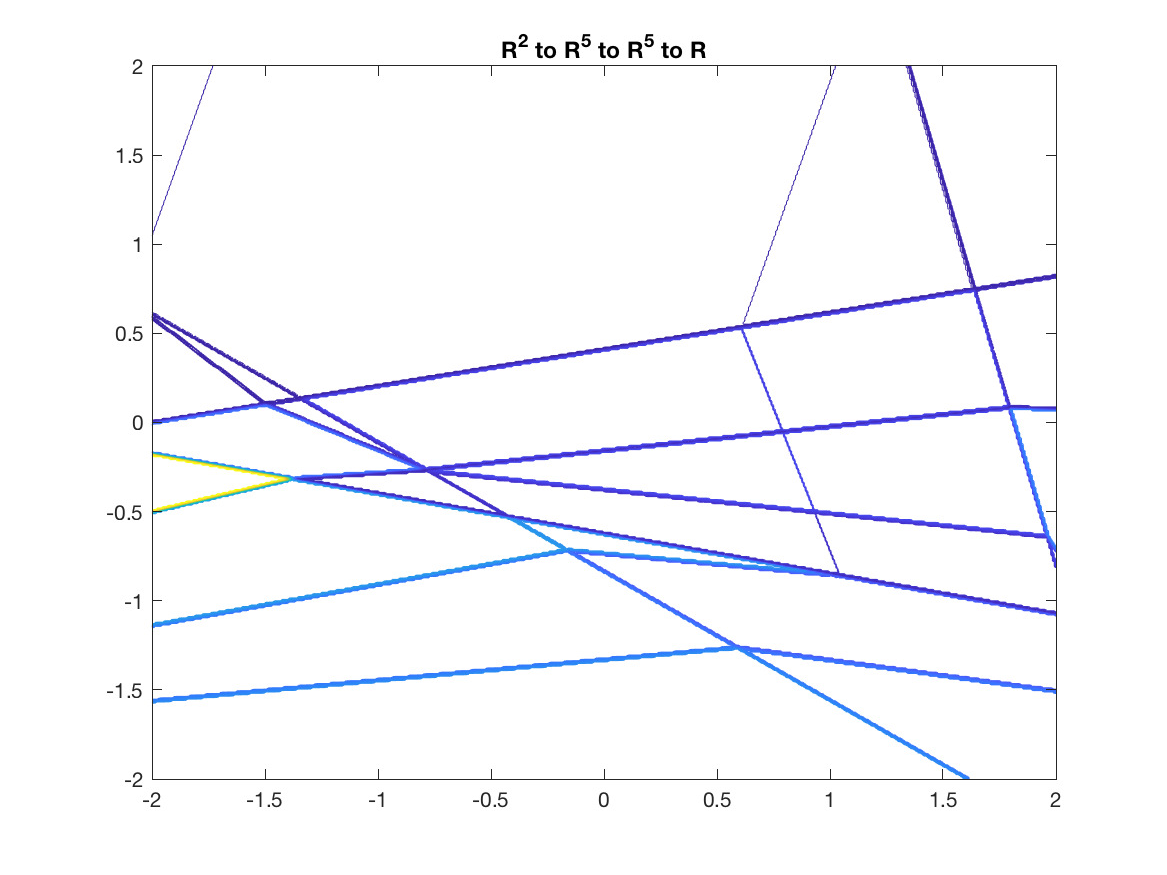
\includegraphics[width=.3\textwidth]{figures/2to5to5to1-eps-converted-to.pdf}  
	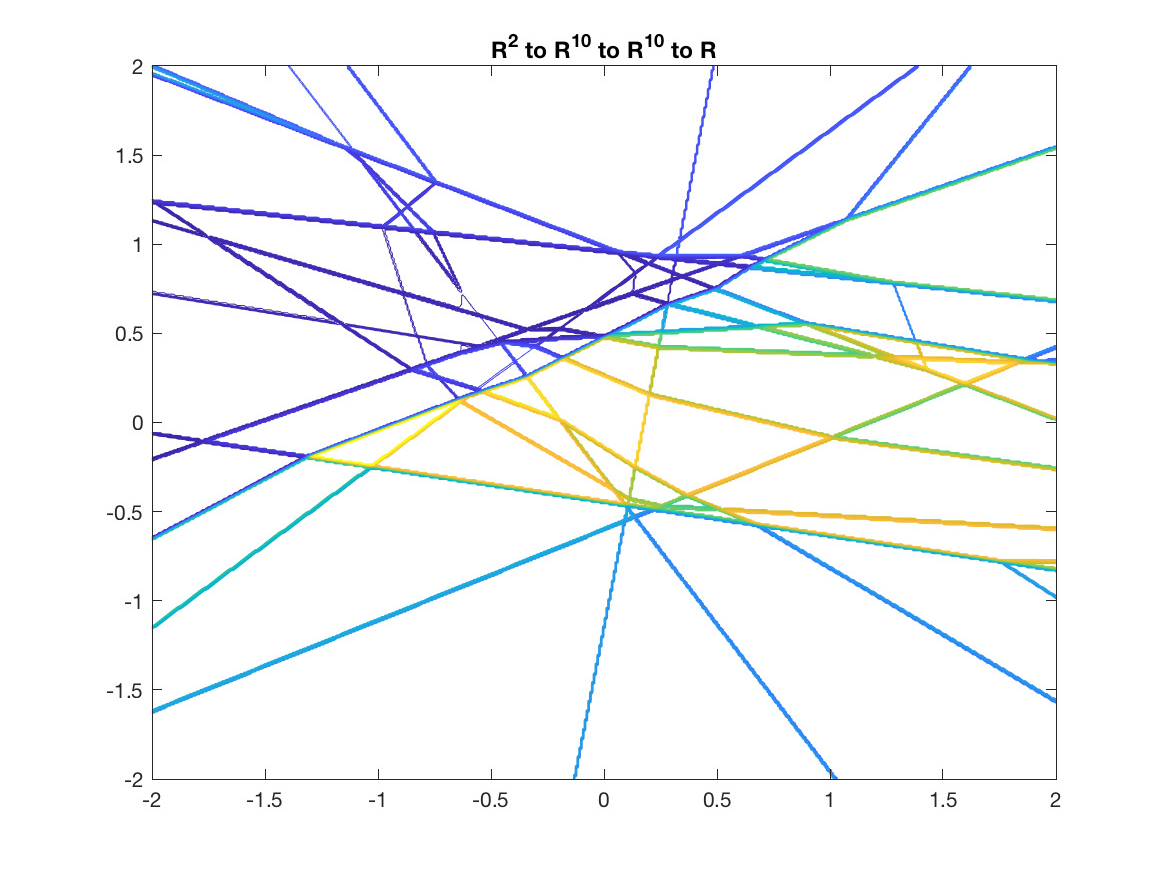
\includegraphics[width=.3\textwidth]{figures/2to10to10to1-eps-converted-to.pdf}  
	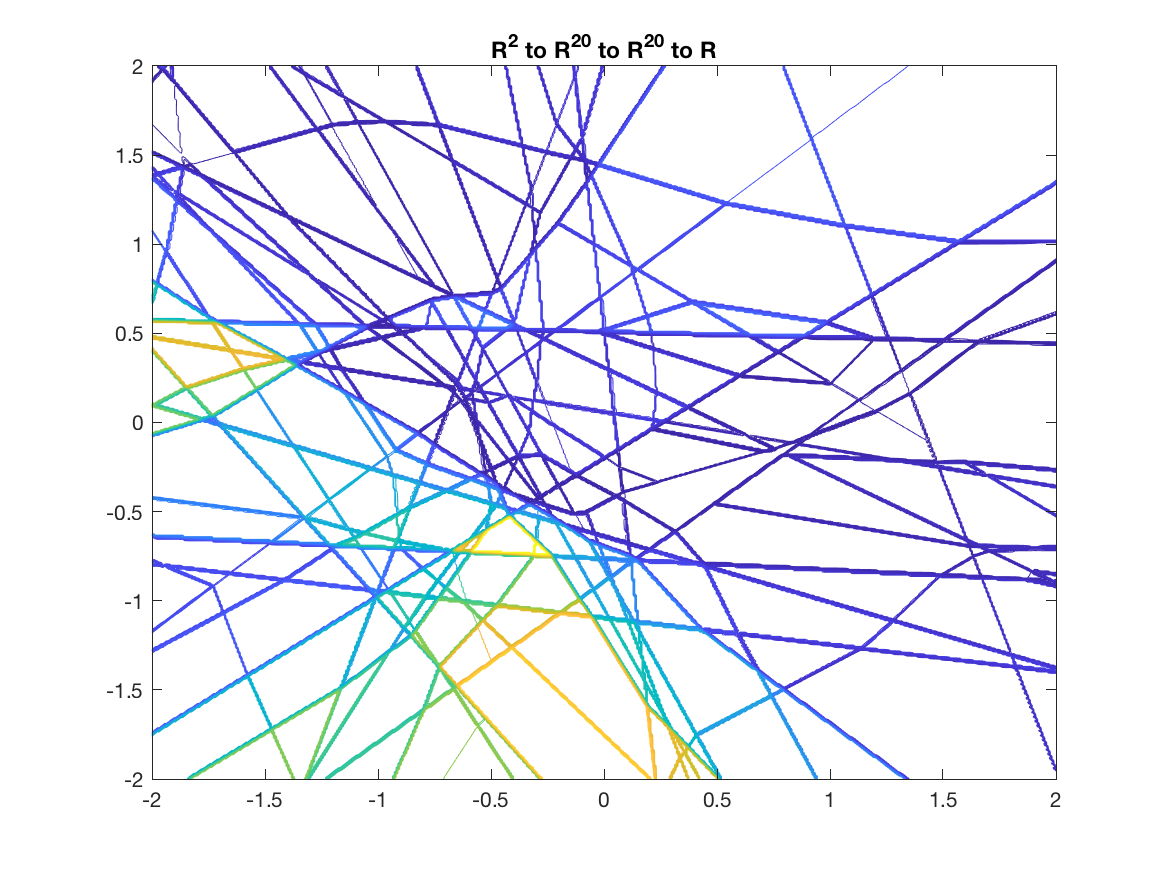
\includegraphics[width=.3\textwidth]{figures/2to20to20to1-eps-converted-to.pdf}  
	\caption{Projections of the domain partitions formed by 2-layer ReLU DNNs with sizes $(n_0, n_1, n_2, n_3)= (2, 5, 5, 1), (2, 10, 10, 1) \text{and}\ (2, 20, 20, 1)$ with random parameters.}
	\label{fig:dnn-region}
\end{figure}

For convenience of exposition,  we introduce the following notation:
%\begin{equation}
%\begin{aligned}
%{\rm{DNN}_L} :=\{& f:f=
%\theta^L \circ {\rm ReLU} \circ \theta^{L-1} \cdots {\rm ReLU}\circ \theta^0(x), \\
%&\theta^\ell \in \mathbb{R}^{n_{\ell} \times (n_\ell+1)}, \quad n^0 = d, \quad n^{L+1} = 1, \quad n^\ell \in \mathbb{N}^+\}.
%\end{aligned}
%\end{equation}
Namely $\dnn^L({\sigma})$ represents the DNN model with $L$ hidden layers and
ReLU activation function with arbitrary size, if $\sigma = {\rm ReLU}$.


%\subsection{Fourier transform of polynomials}
We begin by noting that an activation
function $\sigma$, which satisfies a polynomial growth condition
$|\sigma(x)| \leq C(1 + |x|)^n$ for some constants $C$ and $n$, is a
tempered distribution. As a result, we make this assumption on our
activation functions in the following theorems. We briefly note that
this condition is sufficient, but not necessary (for instance an
integrable function need not satisfy a pointwise polynomial growth
bound) for $\sigma$ to be represent a tempered distribution.

 We begin by studying the convolution of $\sigma$ with a Gaussian mollifier. Let $\eta$ be a Gaussian mollifier
 \begin{equation}
  \eta(x) = \frac{1}{\sqrt{\pi}}e^{-x^2}.
 \end{equation}
Set $\eta_\epsilon=\frac{1}{\epsilon}\eta(\frac{x}{\epsilon})$. Then consider 
\begin{equation}
\label{sigma-epsilon}
\sigma_{\epsilon}(x):=\sigma\ast{\eta_\epsilon}(x)=\int_{\mathbb{R}}\sigma(x-y){\eta_\epsilon}(y)dy
\end{equation}
for a given activation function $\sigma$.
It is clear that $\sigma_{\epsilon}\in C^\infty(\mathbb{R})$. Moreover, by considering the Fourier transform (as a tempered
distribution) we see that
\begin{equation}\label{eq_278}
 \hat{\sigma}_{\epsilon} = \hat{\sigma}\hat{\eta}_{\epsilon} = \hat{\sigma}\eta_{\epsilon^{-1}}.
\end{equation} 


We begin by stating a lemma which characterizes the set of polynomials in terms of their
 Fourier transform.
\begin{lemma}\label{polynomial_lemma} Given a tempered distribution
  $\sigma$,  the following statements are equivalent:
\begin{enumerate}
\item $\sigma$ is a polynomial 
\item $\sigma_\epsilon$ given by \eqref{sigma-epsilon} is a polynomial for any
  $\epsilon>0$. 
\item $\text{\normalfont supp}(\hat{\sigma})\subset \{0\}$. 
\end{enumerate}
\end{lemma}
\begin{proof}
  We begin by proving that (3) and (1) are equivalent.  This follows
  from a characterization of distributions supported at a single point
  (see \cite{strichartz2003guide}, section 6.3). In particular, a
  distribution supported at $0$ must be a finite linear combination of
  Dirac masses and their derivatives.  In particular, if
  $\hat{\sigma}$ is supported at $0$, then
  \begin{equation}
   \hat{\sigma} = \displaystyle\sum_{i=1}^n a_i\delta^{(i)}.
  \end{equation}
  Taking the inverse Fourier transform and noting that the inverse
  Fourier transform of $\delta^{(i)}$ is $c_ix^i$, we see that
  $\sigma$ is a polynomial. This shows that (3) implies (1), for the
  converse we simply take the Fourier transform of a polynomial and
  note that it is a finite linear combination of Dirac masses and
  their derivatives.
  
  Finally, we prove the equivalence of (2) and (3). For this it
  suffices to show that $\hat{\sigma}$ is supported at $0$ iff
  $\hat{\sigma}_\epsilon$ is supported at $0$. This follows from
  equation \ref{eq_278} and the fact that $\eta_{\epsilon^{-1}}$ is
  nowhere vanishing.
\end{proof}

As an application of Lemma \ref{polynomial_lemma}, we give a
simple proof of the result in the next section.   

%
\subsection{Cosine functions as activation function}
Let us use a simple example to motivate the spectral Barron space. Consider a bounded domain $\Omega\subset \mathbb
R^d$ and a real function $u\in L^1(\Omega)$.
Recall the Fourier transform of $u\in L^1(\mathbb{R})$ in Definition~\ref{def:fourier1} and \ref{def:fourier2}. 
This gives the following integral representation of $u$ in terms of the cosine function
\begin{equation}
 \label{eq:reint}
u(x)=Re\int_{\mathbb{R}^d} e^{2\pi i\omega\cdot x} \hat u(\omega)d\omega
= \int_{\mathbb{R}^d}\cos (2\pi (\omega\cdot x + b(\omega))) |\hat u(\omega)|d\omega,
\end{equation}
where $ \hat u(\omega)= e^{2\pi ib(\omega)}|\hat u(\omega)|$. Let 
\begin{equation}
 \label{eq:2}
g(x, \omega) = \cos(2\pi (\omega\cdot x + b(\omega)))\quad \mbox{ and }\quad 
\rho(\omega)= |\hat u(\omega)| . 
\end{equation}
Thus, 
\begin{equation}
\label{int-rep}
u(x)= \int_{\mathbb{R}^d}g(x,\omega) \rho(\omega)d\omega,   
\end{equation}
If
$$
\int_{\mathbb R^d} |\hat u(\omega)|d\omega <\infty,
$$
then $\|\rho\|_{L^1}<\infty$. By applying the Lemma \ref{lem:sample},
there exist $\omega_i\in \mathbb R^d$
such that
\begin{equation}
  \label{eq:3}
\|u-u_N\|_{0,\Omega}\le N^{-1/2}\|\hat u\|_{L^1(\mathbb R^d)}.  
\end{equation}
where
\begin{equation}\label{cosfn}
u_N(x) = {\|\hat u\|_{L^1(\mathbb R^d)}\over N} \sum_{i=1}^N \cos (2\pi(\omega_i\cdot x + b(\omega_i)))
\end{equation}
More generally, we consider the approximation property in $H^m$-norm.
By \eqref{eq:reint},
\begin{equation} 
\partial^\alpha u(x)= \int_{\mathbb{R}^d} \cos^{|\alpha|}(2\pi (\omega\cdot x + b(\omega)))\omega^\alpha |\hat u(\omega)|d\omega,  \quad \forall\ |\alpha|\le m.
\end{equation}
For any positive integer $m$, let 
\begin{equation} \label{eq:gm}
g_m(x,\omega)= {\cos (2\pi (\omega\cdot x + b(\omega)))\over  (1+ \|\omega\|)^m}\quad \mbox{and}\quad \rho_m(\omega)= (1+ \|\omega\|)^m|\hat u(\omega) |,
\end{equation}
where
$$
\| \rho_m\|_{L^1(\mathbb R^d)}=\int_{\mathbb R^d} (1+ \|\omega\|)^m|\hat u(\omega) | d\omega<\infty.
$$
Then, $\displaystyle u(x)=\int_{\mathbb R^d} g_m(x,\omega)\rho_m d\omega = \| \rho_m\|_{L^1(\mathbb R^d)}\mathbb{E}g_m(x,\omega)$. Define
\begin{equation}
u_N(x) = {\|\rho_m\|_{L^1(\mathbb R^d)}\over N} \sum_{i=1}^N g_m(x,\omega_i)
= {\|\rho_m\|_{L^1(\mathbb R^d)}\over N} \sum_{i=1}^N {\cos (2\pi(\omega_i\cdot x + b(\omega_i)))\over (1+\|\omega_i\|)^m}.
\end{equation}
It holds that 
$$
\partial^\alpha (u(x) - u_N(x))={\|\rho_m\|_{L^1(\mathbb R^d)}\over N}\sum_{i=1}^N \mathbb{E} \partial^\alpha (g_m(x,\omega) -  g_m(x,\omega_i)).
$$
By Lemma \ref{MC},
\begin{align}
\mathbb{E}_N \sum_{|\alpha|\le m}\|\partial^\alpha (u(x) - u_N(x))\|_{0, \Omega}^2 
&\le 
\|\rho_m \|_{L^1(\mathbb R^d)}^2\mathbb{E}_N \sum_{|\alpha|\le m}\frac{1}{N^2}\sum_{i=1}^N \left (\mathbb{E} \partial^\alpha (g_m(x,\omega) -  g_m(x,\omega_i))\right )^2
\\
&\le 
{\|\rho_m \|_{L^1(\mathbb R^d)}^2\over N}  \sum_{|\alpha|\le m}\mathbb{E} \left (\partial^\alpha g_m(x,\omega)\right)^2
\end{align}
Note that the definitions of $g_m$ and $\rho_m$ in \eqref{eq:gm} guarantee that 
$$
|\partial^\alpha g_m(x,\omega)|\le 1.
$$
Thus,
$$
\mathbb{E}_N \sum_{|\alpha|\le m}\|\partial^\alpha (u(x) - u_N(x))\|_{0, \Omega}^2 \lesssim {\|\rho_m \|_{L^1(\mathbb R^d)}^2\over N}.
$$
This implies that there exist
$\omega_i\in \mathbb R^d$ such that
\begin{equation}
\label{cosHm}
\|u-u_N\|_{H^m(\Omega)}\lesssim N^{-1/2}\int_{\mathbb{R}^d} (1+ \|\omega\|)^m|\hat u(\omega) | d\omega.  
\end{equation}


Given $v\in L^2(\Omega)$,   consider all the possible extension $v_E:
\mathbb{R}^d \mapsto \mathbb{R}$ with $v_E |_{\Omega} = v$ and define
the spectral  Barron norm for any $s\ge 1$:
	\begin{equation}\label{barron-norm0}
	\|v\|_{B^{s}(\Omega)} = \inf_{v_E |_{\Omega} = v} \int_{\mathbb{R}^d}(1+\|\omega\|)^s|\hat{v}_E(\omega)|d\omega
	\end{equation}
and  spectral  Barron space
\begin{equation}
  \label{Barron}
	B^{s}(\Omega) = \{v\in L^2(\Omega): \|v\|_{B^{s}(\Omega)}<\infty\}.  
\end{equation}

In summary, we have 
\begin{equation} 
\|u-u_N\|_{H^m(\Omega)}\lesssim N^{-1/2}  \|u\|_{B^{m}(\Omega)},
\end{equation}
where $u_N$ is defined in \eqref{cosfn}.


Specifically, we will consider the problem of approximating a function with bounded Barron norm \eqref{barron-norm0} in the Sobolev space $H^m(\Omega)$. Our first step will be to prove a lemma showing that the Sobolev norm is bounded by the Barron norm.

\begin{lemma}\label{smoothness-lemma}
 Let $m \geq 0$ be an integer and $\Omega\subset \mathbb{R}^d$ a bounded domain. Then for any Schwartz function $v$, we have
 \begin{equation}\label{embend}
 \|v\|_{W^{m,\infty}(\Omega)} \lesssim \|v\|_{{B}^m(\Omega)} \lesssim  \|v\|_{H^{m + {d\over 2}+\epsilon}(\Omega)},
 \end{equation}
 where $\epsilon$ is positive.
\end{lemma}
\begin{proof}
Recall the inverse Fourier transform in Definition \ref{def:fourier1}
$$
v(x)=\int \hat{v}(\omega) e^{2 \pi i\omega \cdot x} d \omega.
$$
For any $|\alpha|\le m$,
$$
|\partial^\alpha v|=|(2\pi)^{|\alpha|}\int \hat{v}(\omega) \omega^\alpha e^{2 \pi i\omega \cdot x} d \omega|\le |(2\pi)^{|\alpha|}\int \hat{v}(\omega) \|\omega\|^\alpha e^{2 \pi i\omega \cdot x} d \omega| \lesssim \|v\|_{B^m(\Omega)},
$$ 
which proves $ \|v\|_{W^{m,\infty}(\Omega)} \lesssim \|v\|_{{B}^m(\Omega)}$.

\iffalse
 Let $\chi$ be a Schwartz function satisfying $\chi(x) = 1$ for $x\in \Omega$. Such a function exists because $\Omega$ is bounded. Let $\alpha$ be any multi-index with $|\alpha|\leq m$. Then we have
 \begin{equation}
  \|D^\alpha v\|_{L^2(\Omega)} \leq \|\chi D^\alpha u\|_{L^2(\mathbb{R}^d)} \leq \|\hat\chi * \widehat{D^\alpha v}\|_{L^2(\mathbb{R}^d)}
 \end{equation}
 Now we use Young's inequality to obtain
 \begin{equation}
  \|\hat\chi * \widehat{D^\alpha v}\|_{L^2(\mathbb{R}^d)} \leq \|\hat\chi\|_{L^2(\mathbb{R}^d)}\|\widehat{D^\alpha v}\|_{L^1(\mathbb{R}^d)} \leq \|\hat\chi\|_{L^2(\mathbb{R}^d)}\|v\|_{\mathcal{B}^m(\Omega)}.
 \end{equation}
 Combining this over all multi-indices $\alpha$, we get
 \begin{equation}
  \|u\|_{H^m(\Omega)} \lesssim \|v\|_{\mathcal{B}^m(\Omega)},
 \end{equation}
 as desired. \fi
 
 A version of the second inequality
  in \eqref{embend} and its proof 
can be found in \cite{barron1993universal}. Below is a proof, by 
definition and Cauchy-Schwarz
  inequality, 
\begin{align}
\|v\|_{B^m(\Omega)} =& \inf_{v_E |_{\Omega} = v} \left(\int_{\mathbb{R}^d}(1+\|\omega\|)^m|\hat{v}_E(\omega)|d\omega \right)^2
\\
\le &  \int_{\mathbb{R}^d}(1+\|\omega\|)^{-d - 2\epsilon}d\omega  \inf_{v_E |_{\Omega} = v} 
\int_{\mathbb{R}^d}(1+\|\omega\|)^{d + 2m + 2\epsilon} |\hat{v}_E(\omega)|^2d\omega  
\\
\lesssim &  \inf_{v_E |_{\Omega} = v} 
\int_{\mathbb{R}^d}(1+\|\omega\|)^{d + 2m + 2\epsilon} |\hat{v}_E(\omega)|^2d\omega  
\lesssim \|v\|_{H^{m + {d\over 2}+\epsilon}(\Omega)}.
\end{align}


\end{proof}



\subsection{Cosine function as activation function}
	Consider the Fourier transform:
	\begin{equation}
	  \label{Fourier}
	  \hat f(\omega)=\frac{1}{(2\pi)^d}\int_{\mathbb{R}^d}e^{-i\omega\cdot x}f(x)dx
	  \quad \forall \omega \in \mathbb R^d.
	\end{equation}
	We write  
	$\hat{f}(\omega)=e^{i\beta(\omega)}|\hat{f}(\omega)|$. By Fourier inversion formula,
	\begin{equation}
		\label{eqn1}
		f(x)=\int_{\mathbb{R}^d}e^{i\omega\cdot x}\hat{f}(\omega)d\omega
		=\int_{\mathbb{R}^d}e^{i(\omega\cdot x+\beta(\omega))}|\hat{f}(\omega)|d\omega.
	\end{equation}
Since $f(x)$ is real-valued, it implies that, for $x$
	  \begin{equation}
		\label{key}
		\begin{aligned}
			f(x)
			&={\rm Re}\int_{\mathbb{R}^d}
			e^{i\omega\cdot x} 
			\hat{f}(\omega)d\omega \\
			&={\rm Re}\int_{\mathbb{R}^d}
			e^{i\omega\cdot x}
			e^{i\beta
				(\omega)}|\hat{f}(\omega)|d\omega \\
			&=\int_{\mathbb{R}^d}\cos(\omega\cdot
			x+\beta(\omega))|\hat{f}(\omega)|d\omega.
		\end{aligned}
	\end{equation}
	Then we have 
	\begin{equation}\label{key}
	f(x) =\int_{\mathbb{R}^d}k(x,\omega)d\omega,
	\end{equation}
	with
	\begin{equation}\label{key}
	k(x,\omega) = \cos(\omega\cdot
	x+\beta(\omega))|\hat{f}(\omega)|.
	\end{equation}
	Let 
	$$
	\rho(\omega) = |\hat f(\omega)|,\qquad \lambda(\omega)={\rho(\omega)\over \|\rho(\omega)\|_{L^1}}={\rho(\omega)\over \|\hat f\|_{L^1}}.
	$$ 
	
\begin{theorem}
There exist $\omega_i \in \mathbb{R}^d$, s.t., $G = \mathbb{R}$ and 
\begin{equation}\label{key}
\| f(x) - f_n(x)\|_{L^2} \le \frac{1}{\sqrt{n}} \int_{\mathbb{R}^d} |\hat f(\omega)| d \omega,
\end{equation}
where
\begin{equation}\label{key}
f_n(x)  = \frac{\|\hat f\|_{L^1}}{n} \sum_{i=1}^n \frac{ cos(\omega^*_i \cdot x + \beta^*_i)}{\rho(\omega_i^*)}.
\end{equation}
\end{theorem}
Note that 
\begin{equation}\label{key}
f_n = \frac{\|\hat f\|_{L^1}}{n}\sum_{i=1}^n \frac{ cos(\omega^*_i \cdot x + \beta^*_i)}{\rho(\omega_i^*)} \in \dnn(\cos, n).
\end{equation} 

%\subsection{Double Fourier representation}
Suppose $\Omega$ is bounded and $R$ is the maximum norm of an element of $\Omega$. Then
\begin{equation}
\left|\frac{\omega}{a} \cdot x+b\right| \geq \max \left(0,|b|-\frac{R|\omega|}{|a|}\right).
\end{equation}
Suppose $\boldsymbol{\sigma} \in W^{m, \infty}(\mathbb{R})$ is non-zero and it satisfies the polynomial decay condition
\begin{equation}\label{eq:assdecay}
\left|\sigma^{(k)}(s)\right| \leq C_{p}(1+|s|)^{-p}
\end{equation}
for $0\le k\le m+1$ and some $p> 1$. 
Define
\begin{equation}
h(b,\omega)=\bigg (1+ \max \bigg(0, |b|-{R|\omega|\over |a|}\bigg )\bigg )^{-p}.
\end{equation}
It follows that
\begin{equation}\label{eq:decaypro}
\left|\sigma^{(k)}\left(\frac{\omega}{a} \cdot x+b\right)\right| \leq C_{p}\left(1+\left|\frac{\omega}{a} \cdot x+b\right|\right)^{-p} \leq C_{p}h(b,\omega)
\end{equation}
Moreover,
\begin{equation}
\begin{aligned}
\int_{\mathbb{R}} h(b, \omega) d b &=\int_{|b| \leq \frac{R|\omega|}{|a|}} d b+2 \int_{b>\frac{R|\omega|}{|a|}}\left(1+b-\frac{R|\omega|}{|a|}\right)^{-p} d b \\
&=2 R|a|^{-1}|\omega|+2\left[(1-p)^{-1}\left(1+b-\frac{R|\omega|}{|a|}\right)^{1-p}\right]^{\infty} \\
&=2 R|a|^{-1}|\omega|+\frac{2}{p-1} \leq C_{1}(p, \operatorname{diam}(\Omega), \sigma)(1+|\omega|)
\end{aligned}
\end{equation} 

\begin{theorem}
Let $\Omega\subset \mathbb{R}^d$ be a bounded domain. If the activation function  $\boldsymbol{\sigma} \in W^{m, \infty}(\mathbb{R})$ is non-zero and it satisfies the polynomial decay condition
\begin{equation}\label{eq:assdecay}
\left|\sigma^{(k)}(s)\right| \leq C_{p}(1+|s|)^{-p}
\end{equation}
for $0\le k\le m+1$ and some $p> 1$, we have
\begin{equation}
\inf _{f_{n} \in \Sigma_{d}^{n}(\sigma)}\left\|f-f_{n}\right\|_{H^{m}(\Omega)} \leq|\Omega|^{\frac{1}{2}} C(p, m, \operatorname{diam}(\Omega), \sigma) n^{-\frac{1}{2}-\frac{t}{(2+t)(d+1)}}\|f\|_{\mathscr{B}^{m+1+\varepsilon}}
\end{equation}
where $t=\min (p-1, \varepsilon),$ for any $f \in \mathscr{B}^{m+1+\varepsilon}$
\end{theorem}
\begin{proof}
Let $\theta=(\omega, b)$, $\hat f(\omega)=|\hat f(\omega)| e^{ib(\theta)}$,
\begin{equation}
\lambda(\theta) = {\rho(\theta)\over \|\rho(\theta)\|_{L^1(G)}} \qquad \text{with}\qquad \rho(\theta) = (1+|\omega|)^mh(b,\omega)|\cos b(\theta)| |\hat f(\omega)|.
\end{equation}
The polynomial decay condition \eqref{eq:assdecay} implies that
\begin{equation}\label{eq:rhostratify}
\|\rho(\theta)\|_{L^1(G)}\le  C_1(p, {\rm diam}(\Omega), \sigma)\|f\|_{\mathcal{B}^{m+1}}.
\end{equation}
Define
\begin{equation}
g(x,\theta) = {\|\rho(\theta)\|_{L^1(\Theta)}\over 2\pi |\hat \sigma (a)|(1+|\omega|)^{m}h(b,\omega)} {\rm sgn} (\cos b(\theta))\sigma ({\omega\over a}\cdot x+b).
\end{equation}
Thus
\begin{equation}
f(x)=\int_G g(x,\theta)\lambda(\theta)d\theta
\end{equation}
with $G=\mathbb{R}^d\times \mathbb{R}$. 

Let $G = G_A\cup G_A^c$ with
$$
G_A=\big \{(\omega, b): |b|\le A,\ |\omega|\le {A|a|\over 2R}\big \}.
$$
The interval $[-A,A]$ can be divided into $n_b$ subintervals  $\{G_i^b\}_{i=1}^{n_b}$ such that 
$$
|b - b'|<An^{-{1\over d+1}}\quad b, b'\in G_i^b,\quad 1\leq i\leq n_b
$$ 
for $n_b\ge 2\lceil  n^{1\over d+1}\rceil$. 
The interval $[-{A|a|\over 2R}, {A|a|\over 2R}]$ can be divided into $n_\omega$ subintervals $\{G_i^\omega \}_{i=1}^{n_\omega}$ such that
$$
|\omega_j - \omega'_j| \leq {A|a|\over R}n^{-{1\over d+1}}\qquad  \omega,   \omega' \in G_i^\omega,\quad 1\leq i\leq n_\omega
$$
for $n_\omega\ge \lceil n^{1\over d+1}\rceil$.
The product of these intervals gives the following decomposition 
$$
G_A=\tilde G_1\cup \tilde G_2\cup \cdots \cup \tilde G_M
$$
such that for any $\theta=(\omega, b)$ and $\theta'=(\omega',b')$ in $\tilde G_i$,
\begin{equation}
|b - b'|<An^{-{1\over d+1}}, \quad \|\omega - \omega'\|_{\ell^\infty} \leq {A|a|\over R}n^{-{1\over d+1}}.
\end{equation}
Each $\tilde G_i$ can be divided into two subsets:
\begin{equation}
\tilde G_i^1 = \{\theta\in \tilde G_i: \cos (b(\theta))\ge 0\}\quad \tilde G_i^2 = \{\theta\in \tilde G_i: \cos (b(\theta))\le 0\}.
\end{equation}
This leads to a decomposition of $G_A$ by $G_A=\cup_{i=1}^{2M} G_i$. For any $ \theta, \theta'\in G_i$, 
\begin{equation}
|b - b'|<An^{-{1\over d+1}}, \quad \|\omega - \omega'\|_{\ell^\infty} \leq {A|a|\over R}n^{-{1\over d+1}}, {\rm sgn} (\cos b(\theta))={\rm sgn} (\cos b(\theta')).
\end{equation} 
Denote $G_A^c = G_{2M+1}$. Let $n_i=\lceil \lambda(G_i)n\rceil$ and 
\begin{equation}
f_{n}(x)=\sum_{i=1}^{2 M+1} \frac{\lambda(G_{i})}{n_{i}} \sum_{j=1}^{n_{i}}g(x,\theta_{i,j}).
\end{equation}
According to Theorem \ref{lem:stratifiedapprox},  
\begin{equation} 
\mathbb{E}\left(\left\|f - f_{n}\right\|_{H^{m}(\Omega)}^{2}\right)\le
 \sum_{i=1}^{2M+1}  \frac{\lambda^2(G_i)}{n_{i}}  \sup_{\theta_{i},\theta_{i}'\in G_i} \| g(x,\theta_i) - g(x,\theta_i')\|^2_{H^m(\Omega)}  
\end{equation}

Notice that
\begin{equation}
D_x^\alpha g(x,\theta) = {\|\rho(\theta)\|_{L^1(G)}\over 2\pi |\hat \sigma (a)|(1+|\omega|)^{m}h(b,\omega)|a|^{|\alpha|} }{\rm sgn} (\cos b(\theta))  \omega^\alpha \sigma^{(|\alpha|)} ({\omega\over a}\cdot x+b).
\end{equation}
We first consider $\sup_{\theta,\theta'\in G_i} \| g(x,\theta_i) - g(x,\theta_i')\|^2_{H^m(\Omega)} $ ($1\le i\le 2M$). 
\begin{equation}
| D_x^\alpha \big (g(x,\theta_i) - g(x,\theta_i')\big )|\le |a|^{-|\alpha|}| q(x, \theta_i) - q(x, \theta_i')|
\end{equation}
with 
\begin{equation}
q(x, \theta)=(2 \pi|\hat{\sigma}(a)|)^{-1} \|\rho(\theta)\|_{L^1(G)} \omega^{\alpha}(1+|\omega|)^{-m} h(b, \omega)^{-1} \sigma^{(|\alpha|)}\left(\frac{\omega}{a} \cdot x+b\right).
\end{equation}
We now differentiate $D_x^\alpha g(x,\theta)$ with respect to $\omega$ and $b$, noting that for $|\alpha|\le m$,
\begin{equation}
| (1 + |\omega|)^{-m}\omega^\alpha|,\ |D_\omega \big((1 + |\omega|)^{-m}\omega^\alpha\big ) | \lesssim 1
\end{equation}
\begin{equation}
| h(\omega, b)^{-1}|\le \bigg (1+ \max \bigg(0, |b|-{R|\omega|\over |a|}\bigg )\bigg )^{p}
\end{equation}
\begin{equation}
|D_\omega h(\omega, b)^{-1}|,\ |D_b h(\omega, b)^{-1}|\le \bigg (1+ \max \bigg(0, |b|-{R|\omega|\over |a|}\bigg )\bigg )^{p-1}\le \bigg (1+ \max \bigg(0, |b|-{R|\omega|\over |a|}\bigg )\bigg )^{p}.
\end{equation}
It follows from \eqref{eq:assdecay} that
\begin{equation}
\left|D_{b} q(x, \omega, b)\right| \lesssim C_{p}\left(1+\left|\frac{\omega}{a} \cdot x+b\right|\right)^{-p}\left(1+\max \left(0,|b|-\frac{R|\omega|}{|a|}\right)\right)^{p}\|f\|_{\mathscr{B}^{m+1}}
\lesssim C_{p}\|f\|_{\mathscr{B}^{m+1}}
\end{equation} 
Similarly, we obtain, since $|x| \leq R$
\[
\left|D_{\omega} q(\omega, b, x)\right| \lesssim \frac{R}{|a|}\|f\|_{\mathscr{B}^{m+1}}  
\]
Thus,
\begin{equation}
| D_x^\alpha \big (g(x,\theta_i) - g(x,\theta_i')\big )|\lesssim   A n^{-1 /(d+1)}\|f\|_{\mathscr{B}^{m+1}},
\end{equation}
and
\begin{equation}
\sup_{\theta,\theta'\in G_i} \| g(x,\theta_i) - g(x,\theta_i')\|^2_{H^m(\Omega)} \lesssim   A^2 n^{-2 /(d+1)}|\Omega|^{\frac{1}{2}}\|f\|_{\mathscr{B}^{m+1}},
\end{equation}
 
Consider $\sup_{\theta,\theta'\in G_{2M+1}} \| g(x,\theta_i) - g(x,\theta_i')\|^2_{H^m(\Omega)} $. By \eqref{eq:decaypro},
\begin{equation}
\| D_x^\alpha g(x,\theta)\|_{L^\infty(\Omega)} \le  {\|\rho(\theta)\|_{L^1(G)}\over 2\pi |\hat \sigma (a)||a|^{|\alpha|} } \|{1\over (1+|\omega|)^{m}h(b,\omega)} \omega^\alpha \sigma^{(|\alpha|)} ({\omega\over a}\cdot x+b)\|_{L^\infty(\Omega)}
\le  C_p{\|\rho(\theta)\|_{L^1(G)}\over 2\pi |\hat \sigma (a)||a|^{|\alpha|} }.
\end{equation}
Thus,
\begin{equation}
\sup_{\theta,\theta'\in G_{2M+1}} \| g(x,\theta_i) - g(x,\theta_i')\|^2_{H^m(\Omega)}  
\le 
2\sup_{\theta,\in G_{2M+1}} \| g(x,\theta) \|^2_{H^m(\Omega)}
\le  
2C_p{\|\rho(\theta)\|_{L^1(G)}\over 2\pi |\hat \sigma (a)| }\sum_{|\alpha|\le m}|a|^{-|\alpha|}.
\end{equation}
By \eqref{eq:rhostratify},
\begin{equation}
\sup_{\theta,\theta'\in G_{2M+1}} \| g(x,\theta_i) - g(x,\theta_i')\|^2_{H^m(\Omega)} 
\le |\Omega|  C(p, m, \operatorname{diam}(\Omega), \sigma)\|f\|_{\mathscr{B}^{m+1}}^2.
\end{equation}


The final ingradient we need is a bound on the probability measure of $G_{2M+1}.$ To do this, we break the set $G_{A}^{c}$ into two pieces, $A_{1},$ where $|\omega|>\frac{A|a|}{2 R},$ and $A_{2},$ where $|\omega| \leq \frac{A|a|}{2 R}$ and $|b|>A .$ We get
\[
\lambda(G_{2M+1} ) \leq \frac{1}{I(p, \Omega, \sigma, f)}\left[\int_{A_{1}}(1+|\omega|)^{m} h(b, \omega)|\hat{f}(\omega)| d b d \omega+\int_{A_{2}}(1+|\omega|)^{m} h(b, \omega)|\hat{f}(\omega)| d b d \omega \right]
\]
By integrating out $b,$ we immediately obtain
\[
\int_{A_{1}}(1+|\omega|)^{m} h(b, \omega)|\hat{f}(\omega)| d b d \omega \leq \int_{|\omega|>\frac{A|a|}{2 R}} C_{p}(1+|\omega|)^{m+1}|\hat{f}(\omega)| d \omega \lesssim\|f\|_{\mathscr{B}^{m+1+\varepsilon} }A^{-\varepsilon}
\]
On the other hand, on $A_{2}$ we have $|\omega| \leq \frac{A|a|}{2 R}$ and $|b|>A .$ This implies that
\[
|b|-\frac{R|\omega|}{|a|} \geq \frac{A}{2}
\]
so that for $|\omega| \leq \frac{A|a|}{2 R},$ we have
\[
\int_{|b|>A} h(\omega, b)=\int_{|b|>A}\left(1+\max \left(0,|b|-\frac{R|\omega|}{|a|}\right)\right)^{-p} \leq \int_{|x|>\frac{A}{2}}(1+x)^{-p} \lesssim\left(1+\frac{A}{2}\right)^{1-p}
\]
Integrating in $b \text { and then } \omega, \text { we obtain (recall } A \geq 1)$
\[
\int_{A_{2}}(1+|\omega|)^{m} h(b, \omega)|\hat{f}(\omega)| d b d \omega \lesssim\left(1+\frac{A}{2}\right)^{1-p} \int_{|\omega| \leq \frac{A|a|}{2 R} |}(1+|\omega|)^{m}|\hat{f}(\omega)| d \omega \lesssim\|f\|_{\mathscr{B}^{m+1+\varepsilon}} A^{1-p}
\]
Thus,
\[
\lambda(G_{2M+1} )  \lesssim A^{-\min (p-1, \varepsilon)}
\]
All these estimates lead to
\[
\mathbb{E}(\|f_{n}-f\|_{H^{m}(\Omega)}^{2}) \lesssim
|\Omega| \frac{\|f\|_{\mathscr{B}^{m+1+\varepsilon}}^{2}}{n}\left[A^{-\min (p-1, \varepsilon)}+A^{2} n^{-2 /(d+1)}\right]
\]
Optimizing over $A,$ we obtain, for $A=n^{2 /[(d+1)(2+\min (p-1, \varepsilon))]}$
\[
\mathbb{E} (\|f_{n}-f\|_{H^{m}(\Omega)}^{2} ) \lesssim 
| \Omega\|\| f \|_{\mathscr{S}^{m+1+\varepsilon}}^{2} n^{-1-} \frac{2 \sin (p-1, \varepsilon)}{(d+1)(2+\min (p-1, \varepsilon))}
\]
This bound on the expectation means that there must exist samples $\left(\omega_{i j}, b_{i j}, \eta_{i j}\right)$ such that $\tilde{f}_{n}$ defined by
\[
\|f_{n}-f \|_{H^{m}(\Omega)}^{2} \lesssim
|\Omega|\|f\|_{\mathscr{S}^{m+1+\varepsilon}}^{2} n^{-1-\frac{2 \min (p-1, \varepsilon)}{(d+1)(2+\min (p-1, \varepsilon))}}
\]
Thus we finally get
\[
\inf _{f_{n} \in \Sigma_{d}^{3+1}(\sigma)}\left\|f_{n}-f\right\|_{H^{m}(\Omega)} \leq|\Omega|^{\frac{1}{2}} C(p, m, \operatorname{diam}(\Omega), \sigma)\|f\|_{\mathscr{B}^{m+1+\varepsilon} }n^{{-\frac{1}{2}}-\frac{\min (p-1, \varepsilon)}{(d+1)(2+\min (p-1, \varepsilon))}}
\]
as desired.


\end{proof}



\chapter{Qualitative Approximation Properties of DNN
}\label{ch:approx}

Three categories of approximation theory.
\begin{enumerate}
	\item 
	In Barron's paper, there is a section on the lower bound of
	approximation using linear subspaces. If the basis is fixed, then the
	rate $n^{-1/d}$ is not improvable. The DNN uses a basis adapt to the
	function.
	
	The adaptive FEM we have studied before is indeed using linear
	subspaces. For a given and fixed basis, select the best n term to
	approximate a function. The non-linear approximation theory (by
	DeVore) is to relax the smoothness of function to achieve the optimal
	rate $n^{-1/d}$ but won't improve the rate.
	
	Now the problem is a truly nonlinear approximation problem, even the
	basis can be changed according to $f$. The dimension independent rate
	$n^{-1/2}$ seems also optimal. What we can improve is the
	characterization of the smoothness.
\end{enumerate}

\section{Weierstrass Theorem}  
To approximate any continuous function, a very simple idea is to approximate the function in a polynomial space. 
An important property of this space is that polynomials can approximate any reasonable function!
\begin{itemize}
\item $P_n(\mathbb{R}^d)$ is dense in $C(\Omega)$ [Weierstrass theorem]
\item $P_n(\mathbb{R}^d)$ is dense in all Sobolev spaces: $L^2(\Omega), W^{m,p}(\Omega), \ldots$
\end{itemize}

\begin{theorem}
Let $\Omega\subset R^n$ be a  closed and bounded set. Given any continuous function $f(x)$ on $\Omega$, there exists a sequence of polynomials $\{p_n(x)\}$ such 
that 
\begin{equation}
\displaystyle \lim_{n\rightarrow \infty} \max_{x\in \Omega}|f(x)-p_n(x)|=0
\end{equation}
\end{theorem}
\begin{proof}
Let us first give the proof for $d=1$ and $\Omega=[0,1]$. Given $f:[0,1]\rightarrow R$ be a  continuous function. 

Let
\begin{equation}
\tilde f(x)=f(x)-l(x)
\end{equation}
where $l(x)=f(0)+x(f(1)-f(0))$.
Then $\tilde f(0)=\tilde f(1)=0$. Noting that $l(x)$ is a linear function, hence without lose of generality, we can only consider the 
case $f:[0,1]\rightarrow R$ with $f(0)=f(1)=0$. 
Since $f$ is continuous on the closed interval $[0,1]$, then $f$ is uniformly continuous on $[0,1]$.

First we extend $f$ to be zero outside of $[0,1]$ and obtain $f: R\rightarrow R$, then it is obviously that $f$ is still uniformly continuous. 

Next for $0\le x\le 1$, we construct
\begin{equation}
p_n(x)=\int_{-1}^1f(x+t)Q_n(t)dt=\int_{-x}^{1-x}f(x+t)Q_n(t)dt=\int_{0}^{1}f(t)Q_n(t-x)dt
\end{equation} 
where $Q_n(x)=c_n(1-x^2)^n$ and 
\begin{equation}\label{intq}
\int_{-1}^1 Q_n(x) dx=1.
\end{equation} 
Thus $\{p_n(x)\}$ is a sequence of polynomials. 

Since 
\begin{align}
\int_{-1}^1 (1-x^2)^n dx&=2\int_{0}^1 (1-x^2)^n dx=  2\int_{0}^1 (1-x)^n(1+x)^n dx\\ 
&\ge 2\int_{0}^1 (1-x)^n dx=\frac{2}{n+1}> \frac{1}{n}.
\end{align}
Combing with $\int_{-1}^1 Q_n(x) dx=1$, we obtain $c_n< n$ implying that for any $\delta>0$
 \begin{equation}\label{qest}
 0\le Q_n(x)\le n(1-\delta^2)^n \quad (\delta\le |x|\le 1),
 \end{equation}
so that $Q_n\rightarrow 0$ uniformly in $\delta\le |x|\le 1$ as $n\rightarrow \infty$. 

Given any $\epsilon >0$, since $f$ in uniformly continuous, there exists $\delta>0$ such that for any $|y-x|<\delta$, we have 
\begin{equation}\label{fcont}
|f(y)-f(x)|< \frac{\epsilon}{2}.
\end{equation}
Finally, let $M=\max |f(x)|$, using \eqref{fcont}, \eqref{intq} and \eqref{qest}, we have 
\begin{align}
\big| p_n(x)-f(x)\big|&=\big|\int_{-1}^1(f(x+t)-f(t))Q_n(t)dt\big|\le \int_{-1}^1 \big| f(x+t)-f(t)\big| Q_n(t)dt\\
&\le 2M \int_{-1}^{-\delta} Q_n(t)dt+ \frac{\epsilon}{2}\int_{-\delta}^{\delta} Q_n(t)dt+ 2M\int_{\delta}^1 Q_n(t)dt\\
&\le 4M n(1-\delta^2)^n + \frac{\epsilon}{2}< \epsilon
\end{align}
for all large enough $n$, which proves the theorem. 

The above proof generalize the high dimensional case easily.   We
consider the case that
$$
\Omega=[0,1]^d.
$$
By extension and using cut off function,  W.L.O.G.  that we assume
that $f=0$ on the boundary of $\Omega$ and we then extending this
function to be zero outside of $\Omega$.  

Let us consider the special polynomial functions
\begin{equation}
  \label{Qn}
Q_n(x)=c_n\prod_{k=1}^d(1-x_k^2)  
\end{equation}
Similar proof can then be applied. 
\end{proof}























 
\subsection{Curse of dimensionality}
Number of coefficients for polynomial space $P_n(\mathbb{R}^d)$  is
$$
	N = \binom{d+n}{n} = \frac{(n+d)!}{d!n!}.
$$
For example $n = 100$:
		\begin{table}
			\centering
			\begin{tabular}{|c|c|c|c|}
				\hline
				$d = $&  $2$ &  $4$ & $8$\\
				\hline
				$N=$  & $5\times10^3$ & $4.6\times10^6$  & $3.5\times10^{11}$ 	\\
				\hline
			\end{tabular}
		\end{table}
As the this table shows, the dimension of the polynomial space $P_n(\mathbb{R}^d)$   increases rapidly as the degree $n$ increases. This leads to an extremely large space therefore very expensive to approximate functions in polynomial spaces in high dimensions.
\subsection{Runge's phenomenon}
A natural way to approximate a given function on any interval $[a,b]$ is to use an $n$-degree polynomial $p_n(x)$ by $n+1$ equispaced  points, namely
$$
x_i=a+{b-a\over n},\quad i=0,1,2,\cdots,n.
$$
By Weierstrass' theorem, we expect a more accurate reconstruction of $f(x)$ by using more points. But this is not always true as shown in the following example. 
%Consider the case where one desires to interpolate through $n+1$ equispaced points of a function $f(x)$ using the n-degree polynomial $p_n(x)$ that passes through those points. Naturally, one might expect from Weierstrass' theorem that using more points would lead to a more accurate reconstruction of $f(x)$. However, this particular set of polynomial functions $p_n(x)$ is not guaranteed to have the property of uniform convergence; the theorem only states that a set of polynomial functions exists, without providing a general method of finding one.

Consider the Runge function (a scaled version of the Witch of Agnesi)
$$ 
f(x)=\frac{1}{1+25x^{2}}.
$$
Runge found that if this function is interpolated at equidistant points $x_i$ between $-1$ and $1$ such that:
$$
x_{i}={\frac{2i}{n}}-1,\quad i\in \left\{0,1,\dots ,n\right\}
$$
with a polynomial $p_n(x)$ of degree $\leq n$, the resulting interpolation oscillates toward the ends of the interval, i.e. close to $-1$ and $1$. It can even be proven that the interpolation error increases (without bound) when the degree of the polynomial is increased:

$$\lim_{{n\rightarrow \infty }}\left(\max_{{-1\leq x\leq 1}}|f(x)-p_{n}(x)|\right)=+\infty.$$
This shows that high-degree polynomial interpolation at equidistant points can be troublesome.

\begin{figure}
	\begin{center}
		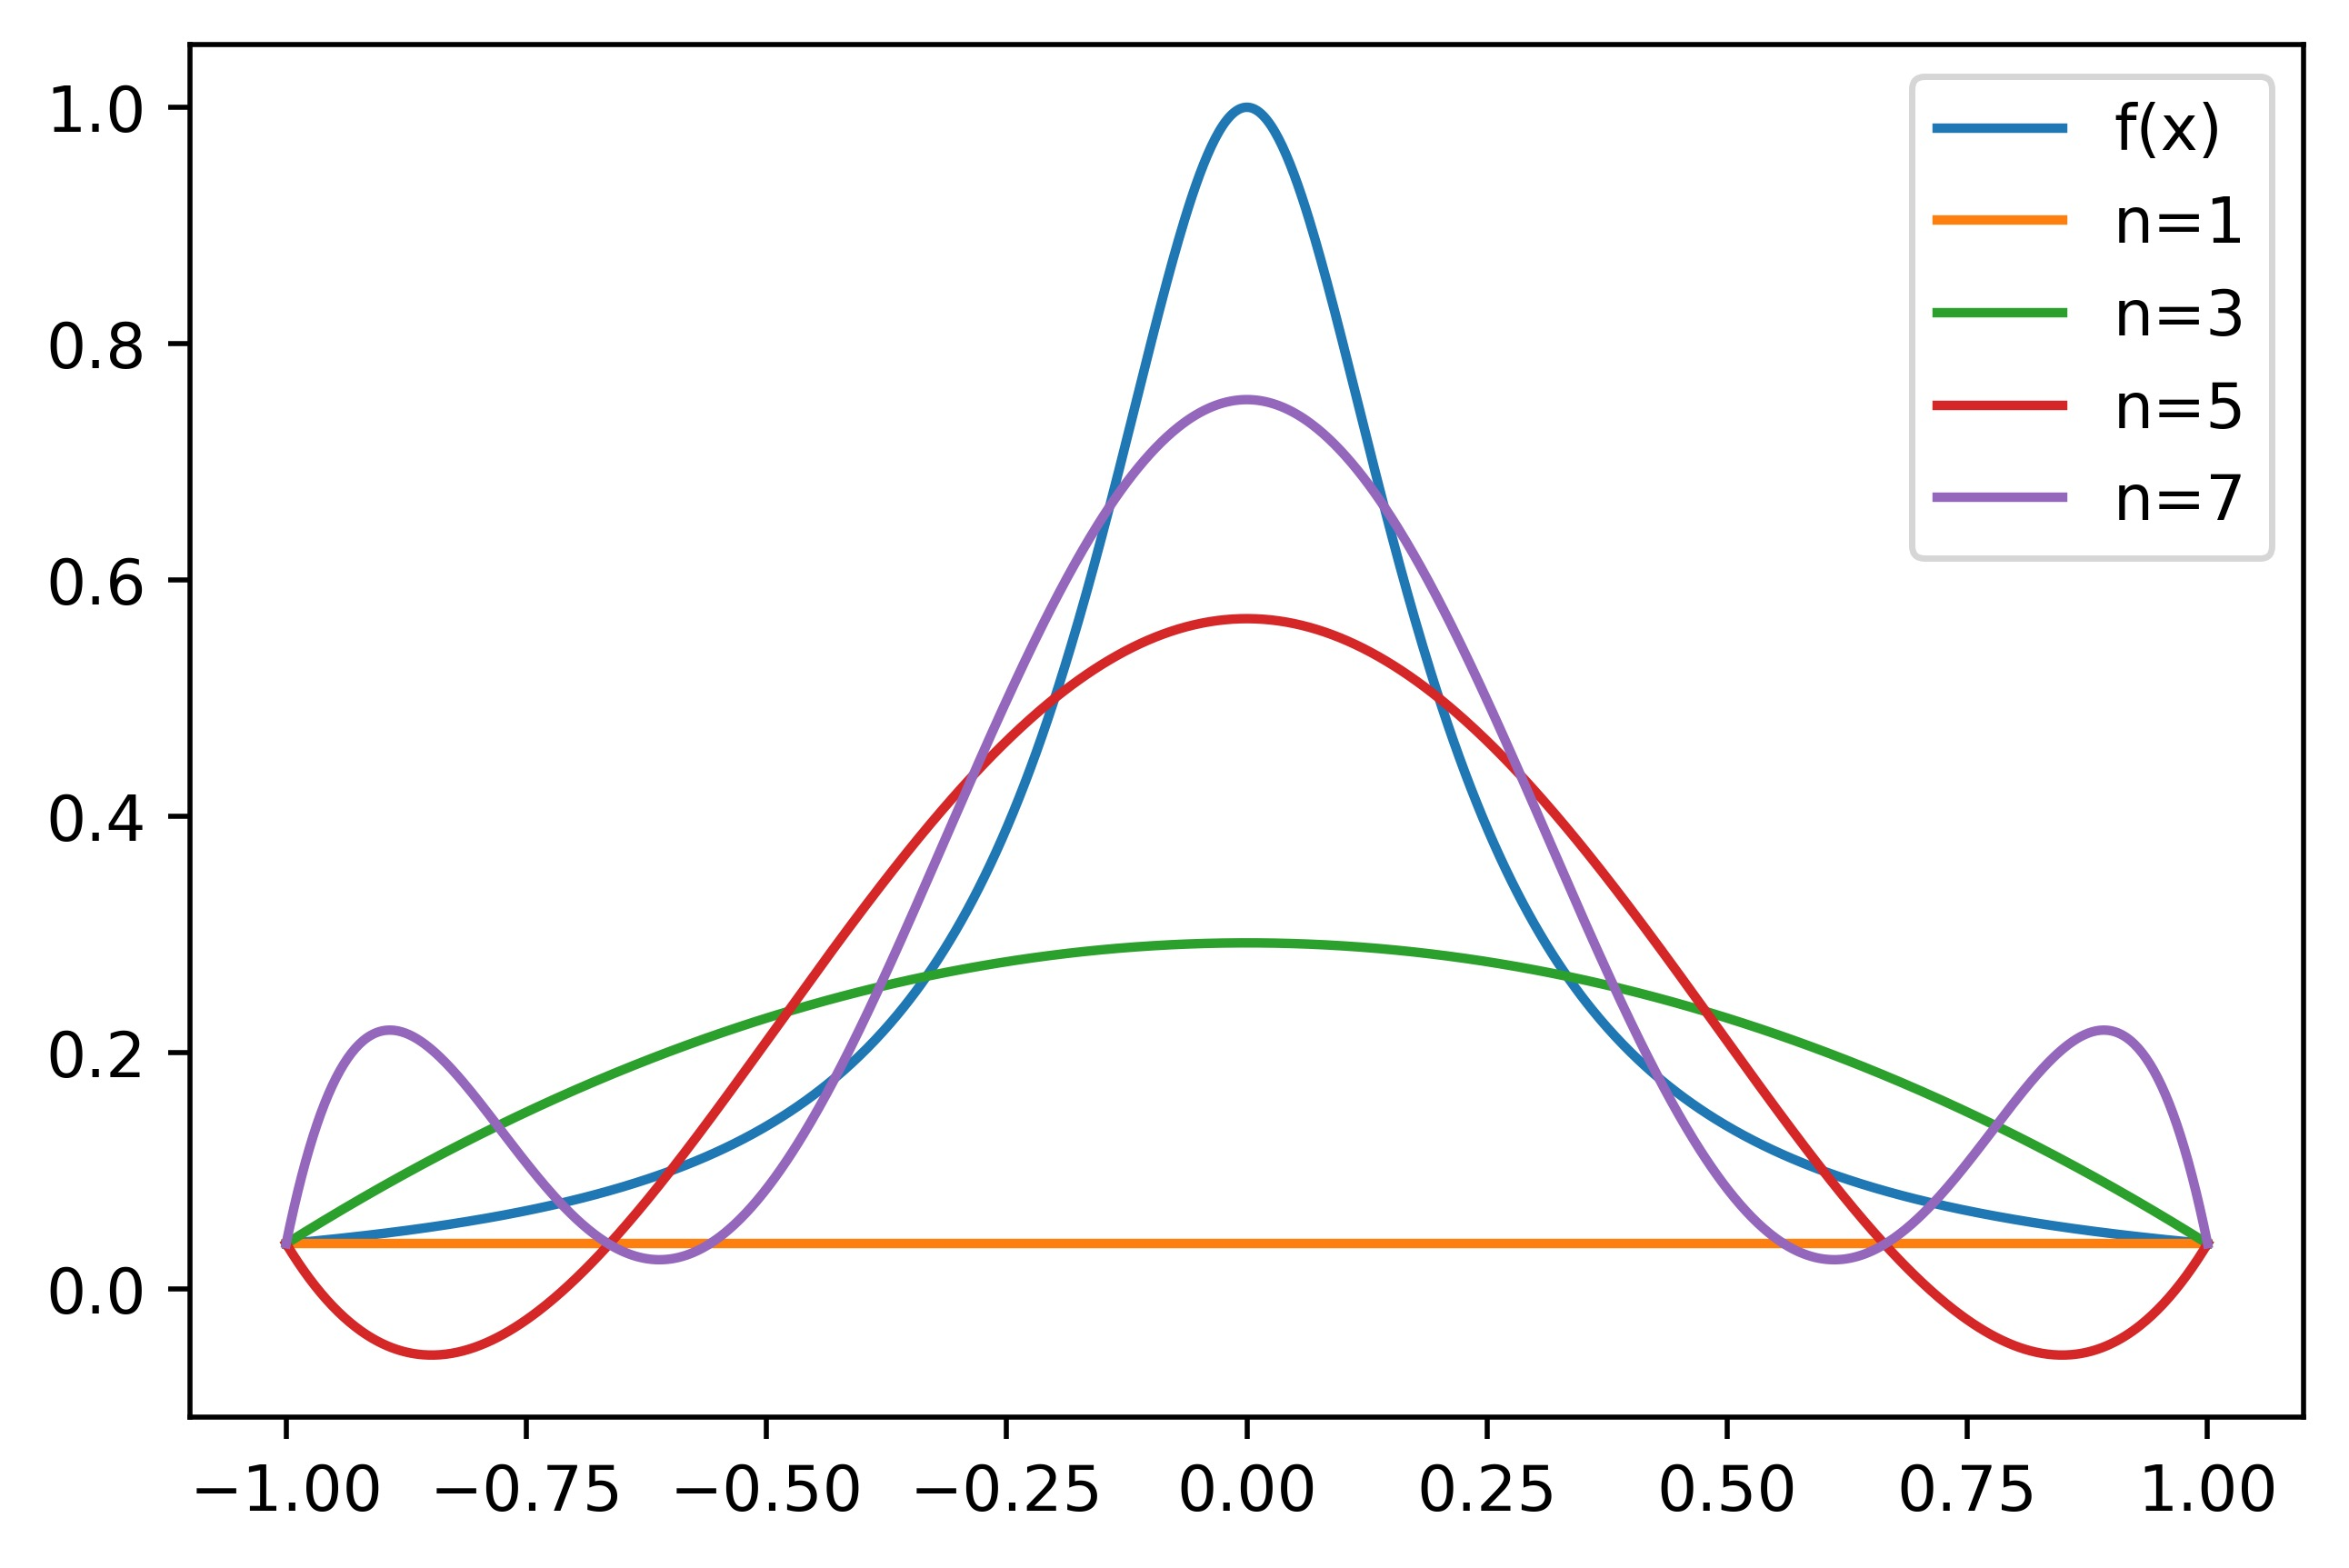
\includegraphics[scale=0.1]{6DL/pic/Runge.jpeg}
		\caption{Runge's phenomenon: Runge function $f(x)=\frac{1}{1+25x^{2}}$ and its polynomial interpolation $p_n(x)$.}
	\end{center}
\end{figure}

The experiment shows that  the polynomials $p_n(x)$ produced in this manner may in fact diverge away from $f(x)$ as $n$ increases. This typically occurs in an oscillating pattern that magnifies near the ends of the interpolation points. This phenomenon is attributed to Runge.

Thus, this particular set of polynomial functions $p_n(x)$ is not guaranteed to have the property of uniform convergence. In other words, Weierstrass' theorem guarantees the existence of the polynomial functions, but how to find such polynomials is not provided.

\section{Fourier transform and Fourier series}
We make use of the theory of tempered distributions (see
\cite{strichartz2003guide} for an introduction)
and we begin by collecting some results of independent interest, which
will also be important later. 
\subsection{Fourier transform}
Before studying the Fourier transform, we first consider Schwartz space which is defined below.
\begin{definition} \label{def:schwarz}
The Schwartz space $\mathcal{S}\left(\mathbb{R}^{n}\right)$ is the topological vector space of functions $f: \mathbb{R}^{n} \rightarrow \mathbb{C}$ such that $f \in C^{\infty}\left(\mathbb{R}^{n}\right)$ and
$$
x^{\alpha} \partial^{\beta} f(x) \rightarrow 0 \quad \text { as }|x| \rightarrow \infty
$$
for every pair of multi-indices $\alpha, \beta \in \mathbb{N}_{0}^{n} .$ For $\alpha, \beta \in \mathbb{N}_{0}^{n}$ and $f \in \mathcal{S}\left(\mathbb{R}^{n}\right)$ let
(5.10)
$$
\|f\|_{\alpha, \beta}=\sup _{\mathbb{R}^{n}}\left|x^{\alpha} \partial^{\beta} f\right|
$$
A sequence of functions $\left\{f_{k}: k \in \mathbb{N}\right\}$ converges to a function $f$ in $\mathcal{S}\left(\mathbb{R}^{n}\right)$ if
$$
\left\|f_{n}-f\right\|_{\alpha, \beta} \rightarrow 0 \quad \text { as } k \rightarrow \infty
$$
for every $\alpha, \beta \in \mathbb{N}_{0}^{n}$.
\end{definition}
The Schwartz space consists of smooth functions whose derivatives and the function itself decay at infinity faster than any power. Schwartz functions are rapidly decreasing. When there is no ambiguity, we will write $\mathcal{S}\left(\mathbb{R}^{n}\right)$ as $\mathcal{S}$.
Roughly speaking, tempered distributions grow no faster than a polynomial at infinity.

\begin{definition}
A tempered distribution $T$ on $\mathbb{R}^{n}$ is a continuous linear functional $T: \mathcal{S}\left(\mathbb{R}^{n}\right) \rightarrow \mathbb{C} .$ The topological vector space of tempered distributions is denoted by $\mathcal{S}^{\prime}\left(\mathbb{R}^{n}\right)$ or $\mathcal{S}^{\prime} .$ If $\langle T, f\rangle$ denotes the value of $T \in \mathcal{S}^{\prime}$ acting on $f \in \mathcal{S}$
then a sequence $\left\{T_{k}\right\}$ converges to $T$ in $\mathcal{S}^{\prime}$, written $T_{k} \rightarrow T$, if
$$
\left\langle T_{k}, f\right\rangle \rightarrow\langle T, f\rangle
$$
for every $f \in \mathcal{S}$.
\end{definition}
Since $\mathcal{D} \subset \mathcal{S}$ is densely and continuously imbedded, we have $\mathcal{S}^{\prime} \subset \mathcal{D}^{\prime} .$ Moreover, a distribution $T \in \mathcal{D}^{\prime}$ extends uniquely to a tempered distribution $T \in \mathcal{S}^{\prime}$ if and only if it is continuous on $\mathcal{D}$ with respect to the topology on $\mathcal{S}$. Every function $f \in L_{\text {loc }}^{1}$ defines a regular distribution $T_{f} \in \mathcal{D}^{\prime}$ by
$$
\left\langle T_{f}, \phi\right\rangle=\int f \phi d x \quad \text { for all } \phi \in \mathcal{D}.
$$
If $|f| \leq p$ is bounded by some polynomial $p,$ then $T_{f}$ extends to a tempered distribution $T_{f} \in \mathcal{S}^{\prime}$, but this is not the case for functions $f$ that grow too rapidly at infinity.

The Schwartz space is a natural one to use for the Fourier transform. Differentiation and multiplication exchange roles under the Fourier transform and therefore so do the properties of smoothness and rapid decrease. As a result, the Fourier transform is an automorphism of the Schwartz space. By duality, the Fourier transform is also an automorphism of the space of tempered distributions.

\begin{definition}\label{def:fourier1}
The Fourier transform of a function $f \in \mathcal{S}\left(\mathbb{R}^{n}\right)$ is the function $\hat{f}: \mathbb{R}^{n} \rightarrow \mathbb{C}$ defined by 
$$
\hat{f}(\omega)= \int f(x) e^{-2 \pi i\omega \cdot x} d x.
$$
The inverse Fourier transform of $f$ is the function $\check{f}: \mathbb{R}^{n} \rightarrow \mathbb{C}$ defined by
$$
\check{f}(x)=\int f(\omega) e^{2 \pi i\omega \cdot x} d k.
$$
\end{definition}

\begin{definition}\label{def:fourier2}
The Fourier transform of a tempered distribution $f \in \mathcal{S}'$ is  defined by 
$$
\langle \hat{f}, \phi\rangle = \langle f, \hat \phi\rangle,\quad \forall \phi\in \mathcal{S}.
$$ 
\end{definition}

The support of a continuous function $f$ is the closure  of the set $\{x\in \mathbb{R}: f(x)\neq 0\}$.
\begin{properties}
The Fourier transform has the following properties
\begin{enumerate}
\item If $f\in \mathcal{S}'$ and the support of $\hat f$ is $\{0\}$, then $f$ is a polynomial.
\item If $f\in \mathcal{S}'$ and the support of $\hat f$ is a single point $\{a\}$, then $f(x)=e^{2\pi iax}P(x)$, where $P(x)$ is a polynomial.
\end{enumerate}
\end{properties}







\subsection{Poisson summation formula}
% Qingguo put the Poisson summation formula here in this file:  statement and sketch of proof

\begin{theorem}
Let $f \in L^{1}(\mathbb{R})$ and $f$ is continuous. Then we have for almost all $(x, \omega ) \in \mathbb{R} \times \hat{\mathbb{R}}$ that
$$
T \sum_{n \in \mathbb{Z}} f(x+n T) e^{-2 \pi i \omega (x+n T)}=\sum_{n \in \mathbb{Z}} \hat{f}\left(\omega +\frac{n}{T}\right) e^{2 \pi i n x / T}
$$
where both sides converge absolutely.

In addition,  let $\Lambda$ be the lattice in $\mathbb{R}^{d}$ consisting of points with integer coordinates. 
For a function $f$ in $L^{1}\left(\mathbb{R}^{d}\right)$ and $f$ is continuous, we have 
$$
\sum_{\omega  \in \Lambda} f(x+\omega )=\sum_{\nu \in \Lambda} \hat{f}(\omega ) e^{2 \pi i x \cdot \omega }.
$$
where both series converge absolutely and uniformly on $\Lambda$. 
\end{theorem} 

\begin{proof}
We just give a proof of a simple case that $f: \mathbb{R} \rightarrow \mathbb{C}$ is a Schwarz function (see Definition \ref{def:schwarz}).
Let:
$$
F(x)=\sum_{n \in \mathbb{Z}} f(x+n).
$$
Then $F(x)$ is 1-periodic (because of absolute convergence), and has Fourier coefficients:
$$
\begin{aligned}
\hat{F}_{\omega } &=\int_{0}^{1} \sum_{n \in \mathbb{Z}} f(x+n) e^{-2 \pi i \omega x} \mathrm{~d} x \\
&=\sum_{n \in \mathbb{Z}} \int_{0}^{1} f(x+n) e^{-2 \pi i \omega  x} \mathrm{~d} x \quad \text { because } f \text { is Schwarz, so convergence is uniform}\\
&=\sum_{n \in \mathbb{Z}} \int_{n}^{n+1} f(x) e^{-2 \pi i\omega  x} \mathrm{~d} x \\
&=\int_{\mathbb{R}} f(x) e^{-2 \pi i \omega  x} \mathrm{~d} x\\
&=\hat{f}(k)\\
\end{aligned}
$$
 where $\hat{f}$ is the Fourier transform of $f$.
 

Therefore by the definition of the Fourier series of $f:$
$$
F(x) =\sum_{\omega  \in \mathbb{Z}} \hat{f}(k) e^{2\pi i \omega x}.
$$
Choosing $x=0$ in this formula:
$$
\sum_{n \in \mathbb{Z}} f(n)=\sum_{\omega  \in \mathbb{Z}} \hat{f}(\omega )
$$
as required.
\end{proof}






\subsection{A special cut-off function}
Let us first state the following simple result that can be obtained by following a calculation given in Section 3 of \cite{johnson2015saddle}. 
\begin{lemma} Given $\alpha>1$, consider
 \begin{equation}\label{alpha-g}
  g(t) = \begin{cases} 
      e^{-(1-t^2)^{1 - \alpha}} & t\in (-1,1) \\
      0 & \text{otherwise}.
   \end{cases}
 \end{equation}
then there is a constant $c_\alpha$ such that
 \begin{equation}\label{eq_181}
  |\hat{g}(\omega )|\lesssim e^{-c_\alpha|\omega |^{1-\alpha^{-1}}},
 \end{equation}
\end{lemma}
\begin{proof}
Consider the asymptotic behavior of the Fourier transform
$$
F(\omega )=\int_{-\infty}^{\infty} g(t) e^{2\pi i \omega  t} dt=2 \operatorname{Re} \int_{0}^{1} e^{2\pi i \omega  t- (1-t^{2})^{1-\alpha}} dt
$$
for $|\operatorname{Re} \omega | \gg 1.$ (Without loss of generality, we can restrict ourselves to real $\omega  \geq 0$).  
With a change of variable $x=1-t$,
$$
F(\omega )=2 \operatorname{Re} \int_{0}^{1} e^{f(x)} dx
$$
with 
$
f(x)=2\pi i \omega  - 2\pi i \omega   x- (2x-x^2)^{1-\alpha}\approx \tilde f(x)+O\left(x^{2-\alpha}\right)
$
and 
$$
\tilde f(x) = 2\pi i \omega  - 2\pi i \omega    x - (2 x)^{1-\alpha}.
$$
The saddle point is the $x=x_0$ where $f'(x_0)=0$. Since
$
\tilde f'(x)=-2\pi i \omega  + (\alpha-1)2^{1-\alpha} x^{-\alpha},
$
$$
x_{0} \approx \tilde x_0=\left (2^{-\alpha} (\alpha-1) / i \omega \pi \right )^{1 / \alpha} \sim \omega ^{-1 / \alpha}.
$$
Therefore $\tilde f(\tilde x_{0}) \sim \omega ^{(\alpha-1) / \alpha}$ asymptotically. The second derivative is 
$$
\tilde f'' (\tilde x_{0} )=-2^{1-\alpha}  \alpha(\alpha-1) \tilde x_{0}^{-\alpha-1}=-i^{(\alpha+1) / \alpha} 2 A \omega ^{(\alpha+1)/\alpha},
$$
where
$$
A=2\alpha  (\alpha-1)^{-1/\alpha}\pi^{(\alpha+1)/\alpha}.
$$
Now,
\begin{equation}
\begin{split}
\tilde f(x)\approx &\tilde f(\tilde x_0) + {\tilde f''(\tilde x_0)\over 2} (x-\tilde x_0)^2
\\
=&2\pi i \omega  - (\alpha - 1)^{1\over \alpha}(i\omega \pi )^{\alpha -1\over \alpha}  - (\alpha - 1)^{1-\alpha\over \alpha} (i\omega \pi )^{\alpha -1\over \alpha}
\\
&-i^{(\alpha+1) / \alpha} A \omega ^{(\alpha+1)/\alpha}(x- 2^{-1}(\alpha - 1)^{-{1\over \alpha}}(i\omega \pi )^{-{1\over \alpha}} )^2.
\end{split}
\end{equation} 
Choose a contour $x=i^{-1 / \alpha}u$, in which case  
$$
\tilde f(x) \approx \tilde f(\tilde x_{0}) -i^{(\alpha-1) / \alpha} A \omega ^{(\alpha+1) / \alpha}\left(u-u_{0}\right)^{2},
$$
which is a path of descent so we can perform a Gaussian integral. 

Recall that the integral of 
\begin{equation}\label{gaussInt}
\int_{-\infty}^{\infty} e^{-a u^{2}} d u=\sqrt{\pi / a}
\end{equation}
as long as Re$a>0,$ which is true here. Note also that, in the limit as $\omega $ becomes large, the integrand becomes zero except close to $u=\sqrt{1 / 2 \omega },$ so we can neglect the rest of the contour and treat the integral over $u$ as going from $-\infty$ to $\infty$. (Thankfully, the width of the Gaussian $\Delta u \sim \omega ^{-3 / 4}$ goes to zero faster than the location of the maximum $u_{0} \sim \omega ^{-1 / 2},$ so we don't have to worry about the $u=0$ origin). Also note that the change of variables from $x$ to $u$ gives us the Jacobian factor for 
$$dx=i^{-1 / \alpha}d u.$$ 
Thus, when all is said and done, we obtain the exact asymptotic form of the Fourier integral for $\omega  \gg 1$: 
\begin{equation}
\begin{split}
F(\omega ) \approx &2 \operatorname{Re}\int_{0}^{1} e^{\tilde f(\tilde x_0) - i^{(\alpha-1) / \alpha} A \omega ^{(\alpha+1) / \alpha}\left(u-u_{0}\right)^{2}} dx
\\
=&2 \operatorname{Re} e^{\tilde f(\tilde x_0)} i^{-1 / \alpha} \int_{-\infty}^{\infty} e^{- i^{(\alpha-1) \over  \alpha} A \omega ^{(\alpha+1) / \alpha}\left(u-u_{0}\right)^{2}} du
\\
=&2 \operatorname{Re} e^{\tilde f(\tilde x_0)} \pi^{1/2}i^{-1 / \alpha}  i^{(1-\alpha) \over  2\alpha} A^{-1/2} \omega ^{-(\alpha+1) / 2\alpha}\qquad \text{ by \eqref{gaussInt}} 
\\
=&2 \operatorname{Re}\left[\sqrt{\frac{\pi}{(i \omega )^{(\alpha+1) / \alpha} A}} e^{\tilde f(\tilde x_0)}\right]
\\
\approx &2 \operatorname{Re}\left[\sqrt{\frac{\pi}{(i \omega )^{(\alpha+1) / \alpha} A}} e^{ 2\pi i \omega - 2\pi i \omega  \tilde x_{0}- \left[\left(2-\tilde x_{0}\right) \tilde x_{0}\right]^{1-\alpha}}\right]
\end{split}
\end{equation}  
with $x_{0}$ and $A$ given above.  Notice that $ \tilde x_0\sim \omega ^{-1 / \alpha}$. Thus,
$$
|F(\omega ) | \approx  e^{-c_\alpha|\omega |^{1-\alpha^{-1}}}.
$$
\end{proof}

\subsection{Fourier transform of polynomials}
We begin by noting that an activation
function $\sigma$, which satisfies a polynomial growth condition
$|\sigma(x)| \leq C(1 + |x|)^n$ for some constants $C$ and $n$, is a
tempered distribution. As a result, we make this assumption on our
activation functions in the following theorems. We briefly note that
this condition is sufficient, but not necessary (for instance an
integrable function need not satisfy a pointwise polynomial growth
bound) for $\sigma$ to be represent a tempered distribution.

 We begin by studying the convolution of $\sigma$ with a Gaussian mollifier. Let $\eta$ be a Gaussian mollifier
 \begin{equation}
  \eta(x) = \frac{1}{\sqrt{\pi}}e^{-x^2}.
 \end{equation}
Set $\eta_\epsilon=\frac{1}{\epsilon}\eta(\frac{x}{\epsilon})$. Then consider 
\begin{equation}
\label{sigma-epsilon}
\sigma_{\epsilon}(x):=\sigma\ast{\eta_\epsilon}(x)=\int_{\mathbb{R}}\sigma(x-y){\eta_\epsilon}(y)dy
\end{equation}
for a given activation function $\sigma$.
It is clear that $\sigma_{\epsilon}\in C^\infty(\mathbb{R})$. Moreover, by considering the Fourier transform (as a tempered
distribution) we see that
\begin{equation}\label{eq_278}
 \hat{\sigma}_{\epsilon} = \hat{\sigma}\hat{\eta}_{\epsilon} = \hat{\sigma}\eta_{\epsilon^{-1}}.
\end{equation} 


We begin by stating a lemma which characterizes the set of polynomials in terms of their
 Fourier transform.
\begin{lemma}\label{polynomial_lemma} Given a tempered distribution
  $\sigma$,  the following statements are equivalent:
\begin{enumerate}
\item $\sigma$ is a polynomial 
\item $\sigma_\epsilon$ given by \eqref{sigma-epsilon} is a polynomial for any
  $\epsilon>0$. 
\item $\text{\normalfont supp}(\hat{\sigma})\subset \{0\}$. 
\end{enumerate}
\end{lemma}
\begin{proof}
  We begin by proving that (3) and (1) are equivalent.  This follows
  from a characterization of distributions supported at a single point
  (see \cite{strichartz2003guide}, section 6.3). In particular, a
  distribution supported at $0$ must be a finite linear combination of
  Dirac masses and their derivatives.  In particular, if
  $\hat{\sigma}$ is supported at $0$, then
  \begin{equation}
   \hat{\sigma} = \displaystyle\sum_{i=1}^n a_i\delta^{(i)}.
  \end{equation}
  Taking the inverse Fourier transform and noting that the inverse
  Fourier transform of $\delta^{(i)}$ is $c_ix^i$, we see that
  $\sigma$ is a polynomial. This shows that (3) implies (1), for the
  converse we simply take the Fourier transform of a polynomial and
  note that it is a finite linear combination of Dirac masses and
  their derivatives.
  
  Finally, we prove the equivalence of (2) and (3). For this it
  suffices to show that $\hat{\sigma}$ is supported at $0$ iff
  $\hat{\sigma}_\epsilon$ is supported at $0$. This follows from
  equation \ref{eq_278} and the fact that $\eta_{\epsilon^{-1}}$ is
  nowhere vanishing.
\end{proof}

As an application of Lemma \ref{polynomial_lemma}, we give a
simple proof of the result in the next section.   


\subsection{Fourier transform of polynomials}
We begin by noting that an activation
function $\sigma$, which satisfies a polynomial growth condition
$|\sigma(x)| \leq C(1 + |x|)^n$ for some constants $C$ and $n$, is a
tempered distribution. As a result, we make this assumption on our
activation functions in the following theorems. We briefly note that
this condition is sufficient, but not necessary (for instance an
integrable function need not satisfy a pointwise polynomial growth
bound) for $\sigma$ to be represent a tempered distribution.

 We begin by studying the convolution of $\sigma$ with a Gaussian mollifier. Let $\eta$ be a Gaussian mollifier
 \begin{equation}
  \eta(x) = \frac{1}{\sqrt{\pi}}e^{-x^2}.
 \end{equation}
Set $\eta_\epsilon=\frac{1}{\epsilon}\eta(\frac{x}{\epsilon})$. Then consider 
\begin{equation}
\label{sigma-epsilon}
\sigma_{\epsilon}(x):=\sigma\ast{\eta_\epsilon}(x)=\int_{\mathbb{R}}\sigma(x-y){\eta_\epsilon}(y)dy
\end{equation}
for a given activation function $\sigma$.
It is clear that $\sigma_{\epsilon}\in C^\infty(\mathbb{R})$. Moreover, by considering the Fourier transform (as a tempered
distribution) we see that
\begin{equation}\label{eq_278}
 \hat{\sigma}_{\epsilon} = \hat{\sigma}\hat{\eta}_{\epsilon} = \hat{\sigma}\eta_{\epsilon^{-1}}.
\end{equation} 


We begin by stating a lemma which characterizes the set of polynomials in terms of their
 Fourier transform.
\begin{lemma}\label{polynomial_lemma} Given a tempered distribution
  $\sigma$,  the following statements are equivalent:
\begin{enumerate}
\item $\sigma$ is a polynomial 
\item $\sigma_\epsilon$ given by \eqref{sigma-epsilon} is a polynomial for any
  $\epsilon>0$. 
\item $\text{\normalfont supp}(\hat{\sigma})\subset \{0\}$. 
\end{enumerate}
\end{lemma}
\begin{proof}
  We begin by proving that (3) and (1) are equivalent.  This follows
  from a characterization of distributions supported at a single point
  (see \cite{strichartz2003guide}, section 6.3). In particular, a
  distribution supported at $0$ must be a finite linear combination of
  Dirac masses and their derivatives.  In particular, if
  $\hat{\sigma}$ is supported at $0$, then
  \begin{equation}
   \hat{\sigma} = \displaystyle\sum_{i=1}^n a_i\delta^{(i)}.
  \end{equation}
  Taking the inverse Fourier transform and noting that the inverse
  Fourier transform of $\delta^{(i)}$ is $c_ix^i$, we see that
  $\sigma$ is a polynomial. This shows that (3) implies (1), for the
  converse we simply take the Fourier transform of a polynomial and
  note that it is a finite linear combination of Dirac masses and
  their derivatives.
  
  Finally, we prove the equivalence of (2) and (3). For this it
  suffices to show that $\hat{\sigma}$ is supported at $0$ iff
  $\hat{\sigma}_\epsilon$ is supported at $0$. This follows from
  equation \ref{eq_278} and the fact that $\eta_{\epsilon^{-1}}$ is
  nowhere vanishing.
\end{proof}

As an application of Lemma \ref{polynomial_lemma}, we give a
simple proof of the result in the next section.   

\chapter{Monte Carlo and Stratified Samplings}
%\subsection{Monte Carlo sampling and analysis}
Let $\lambda\ge 0$ be a probability density function on a domain $G \subset
\mathbb R^D (D\ge 1)$ such that
\begin{equation}\label{density}
\int_{G}\lambda(\theta)d\theta=1.
\end{equation}
We define the expectation and variance as follows
\begin{equation}
\label{E}
\mathbb{E}g:=\int_{G}
g(\theta)\lambda(\theta)d\theta,\qquad
\mathbb{V} g: = \mathbb{E}((g - \mathbb{E} g)^2)= \mathbb{E}(g^2) - (\mathbb{E} g)^2.
\end{equation}
We note that 
$$\displaystyle \mathbb{V} g\le \max_{\theta, \theta'\in G}(g(\theta) - g(\theta'))^2.
$$
For any subset $G_i\subset G$, let
$$
\lambda(G_i)=\int_{G_i}\lambda(\theta)d\theta, \qquad \lambda_i(\theta) = {\lambda(\theta)\over \lambda(G_i)}.
$$
It holds that
$$
\mathbb{E}_Gg= \sum_{i=1}^M \lambda(G_i) \mathbb{E}_{G_i}g.
$$ 
%For each $i$, sample $\theta_i$ is chosen randomly from the probability distribution in $G_i$ with probability $\lambda_i(\theta)$. 
For any function $h(\theta_1,\cdots, \theta_N) : G_1\times G_2\cdots G_N \mapsto \mathbb{R}$, define 
$$\mathbb{E}_{G_i}g=\int_{G_i}g(\theta)\lambda_i(\theta)d\theta$$
 and
\begin{equation}
\label{En}
\mathbb{E}_Nh:=\int_{G_1\times G_2\times\ldots\times G_N}
h(\theta_1,\cdots,\theta_N) \lambda_1(\theta_1) \lambda_2(\theta_2)\ldots \lambda_N(\theta_N)
d\theta_1d\theta_2\ldots d\theta_N.
\end{equation}
For the Monte Carlo method, let $G_i=G$ for all $1\le i\le n$, namely,
\begin{equation} 
\mathbb{E}_Nh:=\int_{G\times G\times\ldots\times G}
h(\theta_1,\cdots,\theta_N) \lambda(\theta_1) \lambda(\theta_2)\ldots \lambda(\theta_N)
d\theta_1d\theta_2\ldots d\theta_N.
\end{equation}


\begin{lemma}   \label{MC}
For any $g\in L^\infty(G)$, we have
  \begin{equation}
  \begin{split}
    \mathbb{E}_n\Big(\mathbb{E}g-\frac1n\sum_{i=1}^n
    g(\omega_i)\Big)^2
    &=\frac{1}{n}\mathbb{V}(g)=\frac{1}{n}\Big(\mathbb{E}(g^2) - \big (\mathbb{E}(g)\big )^2\Big)
    \\
    &=
    \left\{
             \begin{aligned}
    \frac{1}{n}\mathbb{V}(g)
   & \le\frac{1}{n} \sup_{\omega, \omega'\in G} |g(\omega) - g(\omega')|^2
    \\
\frac{1}{n}\Big(\mathbb{E}(g^2) - \big (\mathbb{E}(g)\big )^2\Big)
&\le\frac{1}{n} \mathbb E(g^2)\le \frac{1}{n}\|g\|^2_{L^\infty},
\end{aligned}
\right.
\end{split}
  \end{equation} 
\end{lemma}

\begin{proof}%[Proof of Lemma \ref{MC}]
First note that
 \begin{equation}
    \label{eqn}
    \begin{aligned}
\left(\mathbb{E} g-\frac1N\sum_{i=1}^Ng(\omega_i)\right)^2 
  & 
=\frac{1}{N^2} \left(\sum_{i=1}^N(\mathbb{E} g-g(\omega_i))\right)^2 
  \\
  &=\frac{1}{N^2} \sum_{i,j=1}^N(\mathbb{E} g-g(\omega_i))(\mathbb{E} g-g(\omega_j))
  \\
  &=\frac{I_1}{N^2} +\frac{I_2}{N^2}.
    \end{aligned}
  \end{equation}
with 
\begin{equation}
I_1= \sum_{i=1}^N(\mathbb{E} g-g(\omega_i))^2,\quad I_2=\sum_{i\neq  j}^N\left ((\mathbb{E}g)^2-\mathbb {E}(g)(g(\omega_i)+
g(\omega_j))+g(\omega_i)g(\omega_j))\right).
\end{equation}
Consider $I_1$, for any $i$,
 $$
 \mathbb{E}_N(\mathbb{E} g-g(\omega_i))^2
 =\mathbb{E}(\mathbb{E} g-g)^2 = \mathbb{V}(g).
 $$ 
Thus,
$$
 \mathbb{E}_N (I_1) = n\mathbb{V}(g).
$$
For $I_2$, note that
$$
\mathbb E_N g(\omega_i)=\mathbb E_N g(\omega_j) =\mathbb E(g)
$$
and, for $i\neq j$,
\begin{equation}\label{key}
\begin{aligned}
\mathbb {E}_N ( g(\omega_i)g(\omega_j)) &= 
\int_{G\times G\times\ldots\times G}
g(\omega_i) g(\omega_j) \lambda(\omega_1) \lambda(\omega_2)\ldots \lambda(\omega_N)
d\omega_1d\omega_2\cdots d\omega_N \\
&= \int_{G\times G} g(\omega_i) g(\omega_j) \lambda(\omega_1) 
\lambda(\omega_1) \lambda(\omega_2)
d\omega_1d\omega_2 \\
&= \mathbb {E}_N (
g(\omega_i))\mathbb {E}_n(g(\omega_j))
=[\mathbb E(g)]^2.
\end{aligned}
\end{equation}
Thus
 \begin{equation}
\mathbb{E}_N (I_2) = \mathbb{E}_N \left( \sum_{i\neq j}^N((\mathbb{E}g)^2-\mathbb
  E(g)(\mathbb E(g(\omega_i))+ \mathbb E(g(\omega_j)))+\mathbb E(g(\omega_i)g(\omega_j))) \right)=0.
  \end{equation}
Consequently, there exist the following two formulas for $\displaystyle \mathbb{E}_N\left(\mathbb{E} g-
      \frac1N\sum_{i=1}^Ng(\omega_i)\right)^2$:
 \begin{equation} 
 \mathbb{E}_N\left(\mathbb{E} g-
      \frac1N\sum_{i=1}^Ng(\omega_i)\right)^2 = \frac{1}{N^2}\mathbb{E}_N (I_1)
      =
           \left\{
             \begin{aligned}
            \frac{1}{N}\mathbb{E}\big ((\mathbb{E} g-g)^2\big )\\
            \frac{1}{N}(\mathbb{E}(g^2) - (\mathbb{E} g)^2).
            \end{aligned}
    \right.
  \end{equation}
Based on the first formula above, since
$$
|g(\omega) - \mathbb{E} g|=|\int_G \big (g(\omega) - g(\tilde \omega) \big )\lambda(\tilde \omega)d\tilde \omega|\le \sup_{\omega, \omega'\in G} |g(\omega) - g(\omega')|,
$$
it holds that
 \begin{equation} 
 \mathbb{E}_N\left(\mathbb{E} g-
      {1\over N }\sum_{i=1}^Ng(\omega_i)\right)^2 
            \le\frac{1}{N} \sup_{\omega, \omega\in G} |g(\omega) - g(\omega')|^2.
  \end{equation}
Due to the second formula above,  
 \begin{equation}
    \label{eqn}
 \mathbb{E}_N\left(\mathbb{E} g-
      \frac1N\sum_{i=1}^Ng(\omega_i)\right)^2  
            \le\frac{1}{N} \mathbb E(g^2)\le\frac{1}{N}\|g\|^2_{L^\infty}
  \end{equation}
which completes the proof.
\end{proof}

We can also generalize Lemma \ref{MC} to Hilbert spaces following a similar analysis.

\begin{lemma}    
For any $g: G\rightarrow H$ where $H$ is a Hilbert space, we have
  \begin{equation}
  \begin{split}
    \mathbb{E}_n\Big(\|\mathbb{E}g-\frac1n\sum_{i=1}^n
    g(\omega_i)\|_H^2\Big)
    &=\frac{1}{n}\mathbb{V}(g)=\frac{1}{n}\Big(\mathbb{E}(\|g\|_H^2) - \big (\mathbb{E}(\|g\|_H)\big )^2\Big)
    \\
    &=
    \left\{
             \begin{aligned}
    \frac{1}{n}\mathbb{V}(g)
   & \le\frac{1}{n} \sup_{\omega, \omega'\in G} \|g(\omega) - g(\omega')\|_H^2
    \\
\frac{1}{n}\Big(\mathbb{E}(\|g\|_H^2) - \big (\mathbb{E}(\|g\|_H)\big )^2\Big)
&\le\frac{1}{n} \mathbb E(\|g\|_H^2),
\end{aligned}
\right.
\end{split}
  \end{equation} 
\end{lemma}

\begin{proof}%[Proof of Lemma \ref{MC}]
First note that
 \begin{equation}
    \label{eqn}
    \begin{aligned}
\left\|\mathbb{E} g-\frac1N\sum_{i=1}^Ng(\omega_i)\right\|_H^2 
  & 
=\frac{1}{N^2} \left\|\sum_{i=1}^N(\mathbb{E} g-g(\omega_i))\right\|_H^2 
  \\
  &=\frac{1}{N^2} \sum_{i,j=1}^N\left(\mathbb{E} g-g(\omega_i), \mathbb{E} g-g(\omega_j)\right)
  \\
  &=\frac{I_1}{N^2} +\frac{I_2}{N^2}.
    \end{aligned}
  \end{equation}
with 
\begin{equation}
I_1= \sum_{i=1}^N\|\mathbb{E} g-g(\omega_i)\|_H^2,\quad I_2=\sum_{i\neq  j}^N\left(\mathbb{E} g-g(\omega_i), \mathbb{E} g-g(\omega_j)\right).
\end{equation}
Consider $I_1$, for any $i$,
 $$
 \mathbb{E}_N(\|\mathbb{E} g-g(\omega_i)\|_H^2)
 =\mathbb{E}(\|\mathbb{E} g-g\|_H^2) = \mathbb{V}(g).
 $$ 
Thus,
$$
 \mathbb{E}_N (I_1) = n\mathbb{V}(g).
$$
For $I_2$, note that
$$
\mathbb E_N \|g(\omega_i)\|_H=\mathbb E_N \|g(\omega_j)\|_H =\mathbb E(\|g\|_H)
$$
and, for $i\neq j$,
\begin{equation}\label{key}
\begin{aligned}
\mathbb {E}_N ( g(\omega_i), g(\omega_j)) &= 
\int_{G\times G\times\ldots\times G}
g(\omega_j) g(\omega_j) \lambda(\omega_1) \lambda(\omega_2)\ldots \lambda(\omega_N)
d\omega_1d\omega_2\cdots d\omega_N \\
&= \int_{G\times G} (g(\omega_j) , g(\omega_j) ) 
\lambda(\omega_i) \lambda(\omega_j)
d\omega_id\omega_j \\
&=\left( \mathbb {E}_N (
g(\omega)) , \mathbb {E}_N(g(\omega))\right)
=\|\mathbb E(g)\|_H^2.
\end{aligned}
\end{equation}
Thus
 \begin{equation}
\mathbb{E}_N (I_2) = \mathbb{E}_N \left( \sum_{i\neq j}^N\big(\|\mathbb{E}g\|_H^2-
(\mathbb  E(g), \mathbb E(g(\omega_i))+ \mathbb E(g(\omega_j)))
+ (g(\omega_i), g(\omega_j))\big) \right)=0.
  \end{equation}
Consequently, there exist the following two formulas for $\displaystyle \mathbb{E}_N\left\|\mathbb{E} g-
      \frac1N\sum_{i=1}^Ng(\omega_i)\right\|_H^2$:
 \begin{equation} 
 \mathbb{E}_N\left\|\mathbb{E} g-
      \frac1N\sum_{i=1}^Ng(\omega_i)\right\|_H^2 = \frac{1}{N^2}\mathbb{E}_N (I_1)
      =
           \left\{
             \begin{aligned}
            \frac{1}{N}\mathbb{E}\big (\|\mathbb{E} g-g\|_H^2\big )\\
            \frac{1}{N}(\mathbb{E}(\|g\|_H^2) - \|\mathbb{E} g\|_H^2).
            \end{aligned}
    \right.
  \end{equation}
Based on the first formula above, since
$$
|g(\omega) - \mathbb{E} g|=|\int_G \big (g(\omega) - g(\tilde \omega) \big )\lambda(\tilde \omega)d\tilde \omega|\le \sup_{\omega, \omega'\in G} |g(\omega) - g(\omega')|,
$$
it holds that
 \begin{equation} 
 \mathbb{E}_N\left\|\mathbb{E} g-
      {1\over N }\sum_{i=1}^Ng(\omega_i)\right\|_H^2 
            \le\frac{1}{N} \sup_{\omega, \omega'\in G} \|g(\omega) - g(\omega')\|_H^2.
  \end{equation}
Due to the second formula above,  
 \begin{equation}
    \label{eqn}
 \mathbb{E}_N\left\|\mathbb{E} g-
      \frac1N\sum_{i=1}^Ng(\omega_i)\right\|_H^2  
            \le\frac{1}{N} \mathbb E(\|g\|_H^2),
  \end{equation}
which completes the proof.
\end{proof}


%
Of course, we can use this to prove a high probability result.
\begin{corollary}
 Under the assumptions of the preceding lemma, we have
 \begin{equation}
\mathbb{\bar P}\left [(\mathbb{E}g-\frac1n\sum_{i=1}^n
    g(\omega_i))^2 >\epsilon\right ] 
\le  \frac{1}{n\epsilon}\|g\|^2_{L^\infty}
 \end{equation}
\end{corollary}
\begin{proof}
 \begin{equation}
  \mathbb{\bar P}\left [(\mathbb{E}g-\frac1n\sum_{i=1}^n
    g(\omega_i))^2 >\epsilon\right ] 
\le \epsilon^{-1}
    \mathbb{\bar E}(\mathbb{E}g-\frac1n\sum_{i=1}^n
    g(\omega_i))^2
\le \frac{1}{n\epsilon}\|g\|^2_{L^\infty}. 
 \end{equation}
 
\end{proof}

This corollary implies that the set of $\omega_i$ where the estimate
$n^{-1}\sum_{i=1}^n g(\omega_i)$ is far from the desired value $\mathbb{E}g$
is small.

The practical usefulness of this algorithm depends upon the existence
of a \textit{repeatable} process (for instance some physical process)
which \textit{generates $\omega$ according to a desired distribution
  $\mu$}.

The precise meaning of this last statement is essentially that the
strong law of large numbers holds. Specifically, if
$\omega_1,...,\omega_n,...$ is a infinite sequence generated by the
process, and $A\subset \Omega$ is any a measurable set, then
\begin{equation}
 \lim_{n\rightarrow\infty} \frac{1}{n}\displaystyle\sum_{i=1}^n\chi_A(\omega_i) = \mu(A).
\end{equation}

Generating $n$ independent samples means generating
$\omega_1,...,\omega_n$ from $\mu^n$ according to the above notion.
The existence of a realizable process generating samples from a
probability distribution, and the practical use of such processes is
an interesting topic in the intersection of statistics, physics, and
computer science. In addition, statistics/probability theory studies
how to take samples from one probability distribution and transform
them to samples from another distribution.

\begin{lemma}\label{lem:sample}
\textup{[Monte Carlo Sampling]}
	Consider 
	\begin{equation}
	\label{uv}
	u(x)=\int_{G}g(x,\theta)\rho(\theta)d\theta   = \mathbb E (g)
	\end{equation}
	with $0\le \rho(\theta)\in L^1(G)$. For any $N\ge 1$, there exist $\theta_i^*\in G$ such that
	$$
	\|u-u_N\|_{L^2(\Omega)}^2 
	\le\frac{1}{N}
	\int_G \|g(\cdot,\theta)\|_{L^2(\Omega)}^2\rho(\theta)d\theta = {\|\rho\|_{L^1(G)}\over N}\mathbb E (\|g(\cdot,\theta)\|_{L^2(\Omega)}^2)
	$$
	where  
	$
	\|g(\cdot,\theta)\|_{L^2(\Omega)}^2 = \int_{\Omega} [g(x,\theta)]^2 d\mu(x),
	$
	\begin{equation}\label{fndef} 
	u_N(x)=\frac{\|\rho\|_{L^1(G)}}{N}\sum_{i=1}^N g(x,\theta_i^*).
	\end{equation}

Similarly, if $g(\cdot, \theta)\in H^m(\Omega)$, for any $N\ge 1$, there exist $\theta_i^*\in G_i$ with $f_N$ given in \eqref{fndef} such that
	\begin{equation}\label{eq:hm}
	\|u-u_N\|_{H^m(\Omega)}^2 
	\le 
	\int_G  \|g(\cdot,\theta)\|_{H^m(\Omega)}^2\rho(\theta)d\theta
	=\frac{\|\rho\|_{L^1(G)}}{N} \mathbb E (\|g(\cdot,\theta)\|_{H^m(\Omega)}^2).
	\end{equation}
\end{lemma}

\iffalse
\begin{proof} 
Note that
\begin{equation}
\label{uv}
u(x) = \|\rho\|_{L^1(G)}\mathbb E (g).
\end{equation}
By Lemma \ref{MC},
$$
\mathbb {E}_n\left(\bigg(\mathbb E(g(x,\cdot))
-\frac{1}{N}\sum_{i=1}^N g(x,\theta_i))\bigg)^2
\right)\le {1\over N} \mathbb E (g^2).
$$
By taking integration w.r.t. $x$ on both sides, we get
$$
\mathbb {E}_n\left(h(\theta_1,\theta_2, \cdots, \theta_N)
\right)\le {1\over N} \mathbb {E} \Big(\int_{\Omega} g^2 d\mu(x)\Big),
$$
where 
$$
h(\theta_1,\theta_2, \cdots, \theta_N) =  \int_{\Omega} \bigg(\mathbb E(g(x,\cdot))
-\frac{1}{N}\sum_{i=1}^N g(x,\theta_i))\bigg)^2 d\mu(x).
$$
Since $\mathbb {E}_N (1) = 1$ and $\mathbb {E}_N (h) \le {1\over N} \mathbb {E} \Big(\int_{\Omega} g^2 d\mu(x)\Big)$, there exist $\theta_i^* \in G$ such that
$$
h(\theta_1^*, \theta_2^*, \cdots, \theta_N^*) \le  {1\over N}  \int_{\Omega} \mathbb {E} (g^2) d\mu(x).
$$
%Otherwise, $\mathbb {E}_n\left(h \right) >  {1\over n} \mathbb {E} \Big(\int_{\Omega} g^2 d\mu(x)\Big)$   if $h(\theta_1,\theta_2, \cdots, \theta_n) > {1\over n}  \int_{\Omega} \mathbb {E} (g^2)) d\mu(x)$. 
This implies that
$$
	\mathbb{E}_n\|u-u_N\|_{L^2(\Omega)}^2 
	\le\frac{\|\rho\|_{L^1(G)}}{N}
	\int_G \|g(\cdot,\theta)\|_{L^2(\Omega)}^2\lambda(\theta)d\theta.
	$$ 
	The proof for \eqref{eq:hm} is similar to the above analysis for the $L^2$-error analysis, which completes the proof.
\end{proof}
\fi



We also have a more general version of the above lemma.
\begin{lemma}\label{lem:sampleHk}
	Let 
	\begin{equation} \label{uint}
	u(x)=\int_{G}g(x,\theta)\lambda(\theta)d\theta  = \mathbb E (g)
	\end{equation}
	with $\|\lambda(\theta)\|_{L^1(\Theta)}=1$.
	For any $N\ge 1$, there exist $\theta_i^*\in G$ such that
	$$
	\|u-u_N\|_{H^m(\Omega)}^2 
	\le 
	\int_G  \|g(\cdot,\theta)\|_{H^m(\Omega)}^2\lambda(\theta)d\theta
	=\frac{1}{N} \mathbb E (\|g(\cdot,\theta)\|_{H^m(\Omega)}^2)
	$$
	where 
	$$
	u_N(x)=\frac{1}{N}\sum_{i=1}^N g(x,\theta_i^*)
	$$
	In particular, if 
	\begin{equation}
	\label{eq:4}
	|D^\alpha g(x,\theta)|\le C, \quad\forall x, \theta, |\alpha|\le m
	\end{equation}
	Then
	$$
	\|u-u_N\|_{H^m(\Omega)}
	\le 
	\begin{pmatrix}
	m+d\\
	m
	\end{pmatrix}^{1/2}
	|\Omega|^{1/2}
	N^{-1/2}.
	$$
\end{lemma}

\subsection{Stratified sampling and analysis}
Stratified sampling  \cite{bickel1984asymptotic} gives a more refined version of the Monte Carlo method. 

\begin{lemma} \label{lem:stratified}
 For any
  nonoverlaping decomposition $G=G_1\cup G_2\cup \cdots \cup G_M$ and
  positive integer $n$, let $n_i=\lceil \lambda(G_i)n\rceil$ be the smallest integer larger than $\lambda(G_i)n$ and $\displaystyle N=\sum_{i=1}^M n_i$.  Let $\theta_{i,j}\in G_i (1\le j\le n_i)$ and 
\begin{equation}
g_n=\sum_{i=1}^M \lambda(G_i)g_{n_i}^i \quad \mbox{with}\quad g_{n_i}^i={1 \over n_i}\sum_{j=1}^{n_i} g(\theta_{i,j}).
\end{equation} 
It holds that  
\begin{equation}
\mathbb{E}_N(\mathbb{E}_G g -g_N)^2=\sum_{i=1}^M {\lambda^2(G_i) \over n_i} \mathbb{E}_{G_i}\big (g -\mathbb{E}_{G_i}g\big )^2
\le {1 \over n} \max_{1\le i\le M}\sup_{\theta, \theta'\in G_i}\big |g(\theta) - g(\theta')\big |^2.
\end{equation}
\end{lemma} 

\begin{proof}%[Proof of Lemma \ref{lem:stratified}]
It follows from definition that
\begin{equation}
g(x, \theta) = \sum_{i=1}^M \lambda(G_i) g(x, \theta),\qquad \mathbb{E}_G g =\sum_{i=1}^M\lambda(G_i) \int_{G_i} g\lambda_i(\theta)d\theta = \sum_{i=1}^M \lambda(G_i) \mathbb{E}_{G_i}g.
\end{equation}
Thus, the difference $g - \mathbb{E}_G g$ is a linear combination of $g -\mathbb{E}_{G_i}g$ on each $G_i$ as follows
\begin{equation}
g - \mathbb{E}_G g = \sum_{i=1}^M \lambda(G_i) \big (g -\mathbb{E}_{G_i}g\big ).
\end{equation}
It follows from 
\begin{equation}
\mathbb{E}_G g-g_n=\sum_{i=1}^M \lambda(G_i) (\mathbb{E}_{G_i}g -  g^i_{ n_i})
\end{equation}
and \eqref{En} that
\begin{equation} 
\mathbb{E}_n(\mathbb{E}_G g -g_n)^2 =\sum_{i,j=1}^M \lambda(G_i) \lambda(G_j) \mathbb{E}_n \big ((\mathbb{E}_{G_i}g -  g^i_{ n_i})(\mathbb{E}_{G_j}g -  g^j_{ n_j})\big )
=\sum_{i,j=1}^M \lambda(G_i) \lambda(G_j) I_{ij}  
\end{equation}
with 
$$
I_{ij} = \mathbb{E}_n \big ((\mathbb{E}_{G_i}g -  g^i_{ n_i})(\mathbb{E}_{G_j}g -  g^j_{ n_j})\big ).
$$
\iffalse
If $i\neq j$,
\begin{equation}\label{eq:Iij}
\begin{split}
I_{ij}=&\int_{G\times \cdots\times G} (\mathbb{E}_{G_i}g -  g^i_{ n_i})(\mathbb{E}_{G_j}g -  g^j_{ n_j})\lambda(\theta_{i,n_1})\cdots\lambda(\theta_{i,n_i})\lambda(\theta_{j,1})\cdots \lambda(\theta_{j,n_j})d\theta_{i,1}\cdots d\theta_{i,n_i}d\theta_{j,1}\cdots d\theta_{j,n_j}
\\
=&\int_{G\times \cdots\times G} (\mathbb{E}_{G_i}g -  g^i_{ n_i})\lambda(\theta_{i,n_1})\cdots\lambda(\theta_{i,n_i})d\theta_{i,1}\cdots d\theta_{i,n_i}
\\
&+
\int_{G\times \cdots\times G} (\mathbb{E}_{G_i}g -  g^j_{ n_j})\lambda(\theta_{j,1})\cdots \lambda(\theta_{j,n_j})d\theta_{j,1}\cdots d\theta_{j,n_j}
\\
=&\lambda^{n_i}(G_i)\int_{G_i\times \cdots\times G_i} (\mathbb{E}_{G_i}g -  g^i_{ n_i})\lambda_i(\theta_{i,n_1})\cdots\lambda_i(\theta_{i,n_i})d\theta_{i,1}\cdots d\theta_{i,n_i}
\\
&+
\lambda^{n_j}(G_j)\int_{G\times \cdots\times G} (\mathbb{E}_{G_i}g -  g^j_{ n_j})\lambda_j(\theta_{j,1})\cdots \lambda_j(\theta_{j,n_j})d\theta_{j,1}\cdots d\theta_{j,n_j}
\\
=&0.
\end{split}
\end{equation}
\fi
By Lemma \ref{MC},
\begin{equation}
I_{ij} =  \mathbb{E}_n \big ((\mathbb{E}_{G_i}g -  g^i_{ n_i})^2\big )\delta_{ij}= {1\over n_i} \mathbb{E} \big ((\mathbb{E}_{G_i}g -  g)^2\big )\delta_{ij}.
\end{equation}
Thus,
\begin{equation} 
\mathbb{E}_n(\mathbb{E}_G g -g_n)^2 =\sum_{i=1}^M {\lambda^2(G_i) \over n_i} \mathbb{E}_{G_i}\big (g -\mathbb{E}_{G_i}g\big )^2, 
\end{equation}
which completes the proof.
\end{proof} 

Lemma \ref{MC} and Lemma \ref{lem:stratified} represent two simple identities and subsequent inequalities that can be verified by a direct calculation. Actually Lemma \ref{MC} is a special case of Lemma  \ref{lem:stratified} with $M=1$. Lemma \ref{MC} and Lemma \ref{lem:stratified} are the basis of Monte-Carlo sampling and  stratified sampling in statistics. 

\begin{lemma}\label{lem:stratifiedapprox}
\textup{[Stratified Sampling]}
	For $u(x)$ in \eqref{uint}
	with positive $\rho(\theta)\in L^1(G)$, given any positive integers $n$ and $M\le n$, for  any nonoverlaping decomposition $G=G_1\cup G_2\cup \cdots \cup G_M$, there exists$\{\theta_i^\ast\}_{i=1}^N$ with $n\le N \le 2n$ such that
	\begin{equation} 
	\|u - u_N\|_{L^2(\Omega)} \leq N^{-1/2}\|\rho\|_{L^1(G)}\max_{1\le j\le M}\sup_{\theta_{j},\theta_{j}'\in G_j} \| g(x,\theta_j) - g(x,\theta_j')\|_{L^2(\Omega)} 
	\end{equation}
	where 
	$$
	u_N(x)= {2\|\rho\|_{L^1(G)}\over N}\sum_{i=1}^N\beta_i g(x,\theta_i^\ast)
	$$ 
	and $\beta_i\in [0,1]$.
	\end{lemma}

\begin{proof}
Let $n_j=\lceil \lambda(G_j)n\rceil$ and $\theta_{i,j} \in G_j(1\leq i\leq n_j)$. Define $\displaystyle N=\sum_{j=1}^M n_j$ and
$$
u_N(x)=\|\rho\|_{L^1(G)}\sum_{i=1}^M \lambda(G_i)g_{n_i}^i \quad \mbox{with}\quad g_{n_i}^i={1 \over n_i}\sum_{j=1}^{n_i} g(\theta_{i,j}).
$$
Since
$
\displaystyle u(x)=\|\rho\|_{L^1(G)}\sum_{i=1}^M \lambda(G_i)\mathbb{E}_{G_i} g,
$
by Lemma \ref{MC},
\begin{equation}
\begin{split}
\mathbb{E}_N\|u- u_N \|_{L^2(\Omega)}^2=& \|\rho\|_{L^1(G)}^2
 \sum_{j=1}^{M}{\lambda^2(G_j) \over n_j}\mathbb{E}_{G_j}\|\mathbb{E}_{G_j} g -  g\|^2_{L^2(\Omega)}
\\
\le &\|\rho\|_{L^1(G)}^2 \sum_{j=1}^{M} {\lambda^2(G_j)\over n_j}\sup_{\theta_{j},\theta_{j}'\in G_j} \| g(x,\theta_j) - g(x,\theta_j')\|^2_{L^2(\Omega)}.
\end{split}
\end{equation} 
Since ${\lambda(G_j)\over n_j}\le {1\over n}$ and $\displaystyle \sum_{j=1}^M \lambda(G_j)=1$,
\begin{equation}
\mathbb{E}_N\|u - u_N \|_{L^2(\Omega)}^2\leq n^{-1}\|\rho\|_{L^1(G)}^2\max_{1\le j\le M}\sup_{\theta_{j},\theta_{j}'\in G_j} \| g(x,\theta_j) - g(x,\theta_j')\|^2_{L^2(\Omega)}.
\end{equation}
There exist $\{\theta_{i,j}^\ast\}$ such that $\theta_{i,j}^\ast\in G_i$ and 
\begin{equation}
\| u-u_N \|_{L^2(\Omega)}^2\leq n^{-1} \|\rho\|_{L^1(G)}^2\max_{1\le j\le M}\sup_{\theta_{j},\theta_{j}'\in G_j} \| g(x,\theta_j) - g(x,\theta_j')\|^2_{L^2(\Omega)}.
\end{equation}
Note that $n\le N\le n+M\le 2n$,
$$
u_N(x) =  {2\|\rho\|_{L^1(G)}\over N}\sum_{j=1}^{M}\frac{N\lambda(G_j)}{2n_j}\sum_{i=1}^{n_j} g(x,\theta_{i,j}^\ast)
 =  {2\|\rho\|_{L^1(G)}\over N}\sum_{j=1}^{M}\beta_{i,j}\sum_{i=1}^{n_j} g(x,\theta_{i,j}^\ast)
$$ 
with
\begin{equation}
\beta_{i,j}= \frac{N\lambda(G_j)}{2n_j}\le \frac{2\lambda(G_j)n}{2\lambda(G_j)n}\le 1,
\end{equation}
which completes the proof. 
\end{proof} 



%
\subsection{Stratified sampling}
Stratified sampling refers to a type of sampling method . With stratified sampling, the population is divided into separate groups, called strata. Then, a probability sample (often a simple random sample) is drawn from each group.

Consider the political polling, it's impractical to poll an entire population. So pollsters select a sample of individuals that represents the whole population. Understanding how respondents come to be selected to be in a poll is a big step toward determining how well their views and opinions mirror those of the voting population. A simple example is that choose $n$ individuals randomly,
$$
\mathbb{E}_p({\# Republicans \over n})=p, \quad Var({\# Republicans \over n})=p(1-p).
$$
The accuracy of the sampling is approximate to $\sqrt{p(1-p)\over n}$. If the size of the sample is 100 and $p\approx 0.5$, then $\sqrt{p(1-p)\over n}\approx 5\%$. This implies that the size of the sample should be large enough to get a good estimate.

Another way to select a sample is to break the population into several groups, say A and B. Suppose the percentage of individuals belong to group A is $p_A=70\%$, and the percentage for group B is $p_B=30\%$. And $p_{A, R}=80\%$ individuals in group A will vote for Republicans and only $p_{B, R}=10\%$ in group B will vote for Republicans. Instead of calling $n=100$ individuals randomly, we call $np_A=70$ people in group A and $np_B=30$ people in group B. Then the variance becomes
\begin{equation*}
\begin{split}
\mathbb{V}(0.7{\# Republicans \over 70} + 0.3{\# Republicans \over 30})&=0.7^2{p_{A, R}(1-p_{A, R})\over 70} + 0.3^2{p_{B, R}(1-p_{B, R})\over 30}\\
&=100(0.7*0.8*0.2 + 0.3*0.1*0.9).
\end{split}
\end{equation*}

This is an application of the stratified sampling. The population is divided into separate groups. There are two stratified sampling strategies: One is proportionate allocation, which  uses a sampling fraction in each of the strata that is proportional to that of the total population. The above example belongs to this case. The other strategy is 
optimum allocation, where the sampling fraction of each stratum is proportionate to both the proportion (as above) and the standard deviation of the distribution of the variable. 


Stratified sampling has several advantages over simple random sampling. For example, using stratified sampling, it may improve the precision of the sample by reducing sampling error. It can produce a weighted mean that has less variability than the arithmetic mean of a simple random sample of the population.

Let $\theta$ be a random variable representing the groups mentioned above and $P(\theta)$ be the distribution. Define
$$
f(x)=\mathbb{E}_{P} (f_{\theta}(x))=\mathbb{E}_{\theta} (q(x, \theta))=\int_G q(x,\theta) dP(\theta).
$$ 
A sample from the distribution $P(\theta)$ gives us $\theta_1, \theta_2, \cdots , \theta_n$. Let
\begin{equation}
f_n(x)={1\over n}\sum_{k=1}^n f_{ \theta_k}(x)={1\over n}\sum_{k=1}^n q(x, \theta_k)
\end{equation}
Then, the variance is 
\begin{equation}
\mathbb{V}(f_n(x))={1\over n}\mathbb{V}(f)
\end{equation}
with error ${1\over \sqrt{n}}$.

Stratified sampling is to break $G$ into groups $G_1, G_2, \cdots, G_M$ so that the variation of $q(x,\theta)$ is small on each $G_i$. Instead of sampling uniformly from $G$ and taking the average, we sample from each $G_i$ and get $\theta_{i,1}$, $\theta_{i,2}, \cdots, \theta_{i,n_i}$ where $n_i=\lceil nP(G_i)\rceil$ is the size of samples in $G_i$. Then there exists the estimate
\begin{equation}
\sum_{i=1}^M P(G_i)[{1\over n_i}\sum_{j=1}^{n_i} q(x,\theta_{ij})]
\end{equation}
where ${1\over n_i}\sum_{j=1}^{n_i} q(x,\theta_{ij})$ is an estimate of the conditional expectation $\mathbb{E}_p(q(x,\theta|\theta\in G_i))$. Note that $n_i\leq np_i$ with $p_i=P(G_i)=\int_{G_i} dP(\theta)$. The variance of the estimate is 
\begin{equation}
\sum_{i=1}^M p_i^2{\mathbb{V}[q(x,\theta)|\theta\in G_i)]\over n_i}
\leq \sum_{i=1}^M {p_i^2\over np_i}\mathbb{V}[q(x,\theta)|\theta\in G_i]
= {1\over n}\sum_{i=1}^M p_i\mathbb{V}[q(x,\theta)|\theta\in G_i].
\end{equation} 
This implies that we need to choose $G_i$ so that $\mathbb{V}[q(x,\theta)|\theta\in G_i]$ is small. 

If $G$ is bounded in $\mathbb{R}^d$ and $q(x,\theta)$ is smooth with respect to $\theta$,
$$
|\nabla_\theta q|\leq C.
$$
We can consider a particular partition of $G$ into  $M$ sets $G_1, G_2, \cdots, G_M$ with diameter $\mathcal{O}(n^{-1/d})$. We choose one element from each set. For each $G_i$, sample $n_i=\lceil nP(G_i)\rceil$ samples in $G_i$.  Let
\begin{equation}
f_n(x)=\sum_{k=1}^n p_i[{1\over n_i}\sum_{j=1}^{n_i}q(x,\theta_{ij})]\in NN_{2n}.
\end{equation}
The variance is 
\begin{equation}
Var(f_n)= {1\over n}\sum_{i=1}^M p_i\mathbb{V}[q(x,\theta)|\theta\in G_i]\leq (n^{-1/d}C)^2
\end{equation}
According to , there exists the following modified estimate 
\begin{equation}
Var(f_n)\leq n^{-1-2/d} 
\end{equation}
Thus, for any $f$, there exist $\theta_{ij}, 1\leq i\leq n, 1\leq j\leq n_i$ such that
\begin{equation}
|f_n-f|\leq  n^{-1/2-1/d}.
\end{equation}

 
\begin{lemma}\label{lem:stratifiedapprox}
	Let 
	\begin{equation}
	\label{uv}
	u(x)=\int_{G}g(x,\theta)\lambda(\theta)d\theta  
	\end{equation}
	with $\int_G \lambda(\theta) d\theta=1$. Given any positive integers $N$ and $M\le CN$, for  any decomposition of $G=\cup_{i=1}^M G_i$, there exists $\{\theta_i^\ast\}_{i=1}^N$ such that
	\begin{equation} 
	\|u-u_N|_{L^2(\Omega)} \leq N^{-1/2}\max_{1\le j\le M}\sup_{\theta_{j},\theta_{j}'\in G_j} \| g(x,\theta_j) - g(x,\theta_j')\|_{L^2(\Omega)} 
	\end{equation}
	where 
	$$
	u_N(x)= {1\over N}\sum_{i=1}^N\beta_i g(x,\theta_i^\ast)
	$$ 
	and $\beta_i\in [0,C+1]$.
	\end{lemma}

\begin{proof}
Let $n_j=\lceil \lambda(G_j)n\rceil$ and $\theta_{i,j} \in G_j(1\leq i\leq n_j)$. Define 
$$
u_n(x)=\sum_{i=1}^M \lambda(G_i)g_{n_i}^i \quad \mbox{with}\quad g_{n_i}^i={1 \over n_i}\sum_{j=1}^{n_i} g(\theta_{i,j}).
$$
Since
$
u(x)=\mathbb{E}_G g,
$
by Lemma \ref{MC},
\begin{equation}
\begin{split}
\mathbb{E}_n\| u - u_n \|_{L^2(\Omega)}^2=& 
 \sum_{j=1}^{M}{\lambda^2(G_j) \over n_j}\mathbb{E}_{G_j}\|\mathbb{E}_{G_j} g -  g\|^2_{L^2(\Omega)}
\\
\le & \sum_{j=1}^{M} {\lambda^2(G_j)\over n_j}\sup_{\theta_{j},\theta_{j}'\in G_j} \| g(x,\theta_j) - g(x,\theta_j')\|^2_{L^2(\Omega)}.
\end{split}
\end{equation} 
Since ${\lambda(G_j)\over n_j}\le {1\over n}$ and $\displaystyle \sum_{j=1}^M \lambda(G_j)=1$,
\begin{equation}
\mathbb{E}_n\| u - u_n \|_{L^2(\Omega)}^2\leq n^{-1}\max_{1\le j\le M}\sup_{\theta_{j},\theta_{j}'\in G_j} \| g(x,\theta_j) - g(x,\theta_j')\|^2_{L^2(\Omega)}.
\end{equation}
There exist $\{\theta_{i,j}^\ast\}$ such that $\theta_{i,j}^\ast\in G_i$ and 
\begin{equation}
\| u -  u_n \|_{L^2(\Omega)}^2\leq n^{-1} \max_{1\le j\le M}\sup_{\theta_{j},\theta_{j}'\in G_j} \| g(x,\theta_j) - g(x,\theta_j')\|^2_{L^2(\Omega)}.
\end{equation}
Suppose $\displaystyle N=\sum_{j=1}^M n_j$, $n\le N\le n+M\le (C+1)n$,
$$
u_N(x) =  {1\over N}\sum_{j=1}^{M}\frac{N\lambda(G_j)}{n_j}\sum_{i=1}^{n_j} g(x,\theta_{i,j}^\ast)
 =  {1\over N}\sum_{j=1}^{M}\beta_{i,j}\sum_{i=1}^{n_j} g(x,\theta_{i,j}^\ast)
$$ 
with
\begin{equation}
\beta_{i,j}= \frac{N\lambda(G_j)}{n_j}\le \frac{\lambda(G_j)(C+1)n}{\lambda(G_j)n}\le C+1,
\end{equation}
which completes the proof. 
\end{proof}
\begin{remark}
For the above lemma, there exists $\{\theta_i^\ast\}_{i=1}^N$ such that
	\begin{equation} 
	\|u-u_N\|_{L^2(\Omega)} \leq N^{-1/2}\max_{1\le j\le M}\sup_{\theta_{j},\theta_{j}'\in G_j} \| g(x,\theta_j) - g(x,\theta_j')\|_{L^2(\Omega)} 
	\end{equation}
	where 
$$
	u_N(x)= {C+1\over n}\sum_{i=1}^N\beta_i g(x,\theta_i^\ast)
	$$ 
	and $\beta_i\in [0,1]$.
\end{remark}




\section{Sampling Techniques}
Let $\lambda\ge 0$ be a probability density function on a domain $G \subset
\mathbb R^D (D\ge 1)$ such that
\begin{equation}\label{density}
\int_{G}\lambda(\theta)d\theta=1.
\end{equation}
We define the expectation and variance as follows
\begin{equation}
\label{E}
\mathbb{E}g:=\int_{G}
g(\theta)\lambda(\theta)d\theta,\qquad
\mathbb{V} g: = \mathbb{E}((g - \mathbb{E} g)^2)= \mathbb{E}(g^2) - (\mathbb{E} g)^2.
\end{equation}
We note that 
$$\displaystyle \mathbb{V} g\le \max_{\theta, \theta'\in G}(g(\theta) - g(\theta'))^2.
$$
For any subset $G_i\subset G$, let
$$
\lambda(G_i)=\int_{G_i}\lambda(\theta)d\theta, \qquad \lambda_i(\theta) = {\lambda(\theta)\over \lambda(G_i)}.
$$
It holds that
$$
\mathbb{E}_Gg= \sum_{i=1}^M \lambda(G_i) \mathbb{E}_{G_i}g.
$$ 
%For each $i$, sample $\theta_i$ is chosen randomly from the probability distribution in $G_i$ with probability $\lambda_i(\theta)$. 
For any function $h(\theta_1,\cdots, \theta_N) : G_1\times G_2\cdots G_N \mapsto \mathbb{R}$, define 
$$\mathbb{E}_{G_i}g=\int_{G_i}g(\theta)\lambda_i(\theta)d\theta$$
 and
\begin{equation}
\label{En}
\mathbb{E}_Nh:=\int_{G_1\times G_2\times\ldots\times G_N}
h(\theta_1,\cdots,\theta_N) \lambda_1(\theta_1) \lambda_2(\theta_2)\ldots \lambda_N(\theta_N)
d\theta_1d\theta_2\ldots d\theta_N.
\end{equation}
For the Monte Carlo method, let $G_i=G$ for all $1\le i\le n$, namely,
\begin{equation} 
\mathbb{E}_Nh:=\int_{G\times G\times\ldots\times G}
h(\theta_1,\cdots,\theta_N) \lambda(\theta_1) \lambda(\theta_2)\ldots \lambda(\theta_N)
d\theta_1d\theta_2\ldots d\theta_N.
\end{equation}

\subsection{Monte Carlo sampling and analysis}
Let $\lambda\ge 0$ be a probability density function on a domain $G \subset
\mathbb R^D (D\ge 1)$ such that
\begin{equation}\label{density}
\int_{G}\lambda(\theta)d\theta=1.
\end{equation}
We define the expectation and variance as follows
\begin{equation}
\label{E}
\mathbb{E}g:=\int_{G}
g(\theta)\lambda(\theta)d\theta,\qquad
\mathbb{V} g: = \mathbb{E}((g - \mathbb{E} g)^2)= \mathbb{E}(g^2) - (\mathbb{E} g)^2.
\end{equation}
We note that 
$$\displaystyle \mathbb{V} g\le \max_{\theta, \theta'\in G}(g(\theta) - g(\theta'))^2.
$$
For any subset $G_i\subset G$, let
$$
\lambda(G_i)=\int_{G_i}\lambda(\theta)d\theta, \qquad \lambda_i(\theta) = {\lambda(\theta)\over \lambda(G_i)}.
$$
It holds that
$$
\mathbb{E}_Gg= \sum_{i=1}^M \lambda(G_i) \mathbb{E}_{G_i}g.
$$ 
%For each $i$, sample $\theta_i$ is chosen randomly from the probability distribution in $G_i$ with probability $\lambda_i(\theta)$. 
For any function $h(\theta_1,\cdots, \theta_N) : G_1\times G_2\cdots G_N \mapsto \mathbb{R}$, define 
$$\mathbb{E}_{G_i}g=\int_{G_i}g(\theta)\lambda_i(\theta)d\theta$$
 and
\begin{equation}
\label{En}
\mathbb{E}_Nh:=\int_{G_1\times G_2\times\ldots\times G_N}
h(\theta_1,\cdots,\theta_N) \lambda_1(\theta_1) \lambda_2(\theta_2)\ldots \lambda_N(\theta_N)
d\theta_1d\theta_2\ldots d\theta_N.
\end{equation}
For the Monte Carlo method, let $G_i=G$ for all $1\le i\le n$, namely,
\begin{equation} 
\mathbb{E}_Nh:=\int_{G\times G\times\ldots\times G}
h(\theta_1,\cdots,\theta_N) \lambda(\theta_1) \lambda(\theta_2)\ldots \lambda(\theta_N)
d\theta_1d\theta_2\ldots d\theta_N.
\end{equation}


\begin{lemma}   \label{MC}
For any $g\in L^\infty(G)$, we have
  \begin{equation}
  \begin{split}
    \mathbb{E}_n\Big(\mathbb{E}g-\frac1n\sum_{i=1}^n
    g(\omega_i)\Big)^2
    &=\frac{1}{n}\mathbb{V}(g)=\frac{1}{n}\Big(\mathbb{E}(g^2) - \big (\mathbb{E}(g)\big )^2\Big)
    \\
    &=
    \left\{
             \begin{aligned}
    \frac{1}{n}\mathbb{V}(g)
   & \le\frac{1}{n} \sup_{\omega, \omega'\in G} |g(\omega) - g(\omega')|^2
    \\
\frac{1}{n}\Big(\mathbb{E}(g^2) - \big (\mathbb{E}(g)\big )^2\Big)
&\le\frac{1}{n} \mathbb E(g^2)\le \frac{1}{n}\|g\|^2_{L^\infty},
\end{aligned}
\right.
\end{split}
  \end{equation} 
\end{lemma}

\begin{proof}%[Proof of Lemma \ref{MC}]
First note that
 \begin{equation}
    \label{eqn}
    \begin{aligned}
\left(\mathbb{E} g-\frac1N\sum_{i=1}^Ng(\omega_i)\right)^2 
  & 
=\frac{1}{N^2} \left(\sum_{i=1}^N(\mathbb{E} g-g(\omega_i))\right)^2 
  \\
  &=\frac{1}{N^2} \sum_{i,j=1}^N(\mathbb{E} g-g(\omega_i))(\mathbb{E} g-g(\omega_j))
  \\
  &=\frac{I_1}{N^2} +\frac{I_2}{N^2}.
    \end{aligned}
  \end{equation}
with 
\begin{equation}
I_1= \sum_{i=1}^N(\mathbb{E} g-g(\omega_i))^2,\quad I_2=\sum_{i\neq  j}^N\left ((\mathbb{E}g)^2-\mathbb {E}(g)(g(\omega_i)+
g(\omega_j))+g(\omega_i)g(\omega_j))\right).
\end{equation}
Consider $I_1$, for any $i$,
 $$
 \mathbb{E}_N(\mathbb{E} g-g(\omega_i))^2
 =\mathbb{E}(\mathbb{E} g-g)^2 = \mathbb{V}(g).
 $$ 
Thus,
$$
 \mathbb{E}_N (I_1) = n\mathbb{V}(g).
$$
For $I_2$, note that
$$
\mathbb E_N g(\omega_i)=\mathbb E_N g(\omega_j) =\mathbb E(g)
$$
and, for $i\neq j$,
\begin{equation}\label{key}
\begin{aligned}
\mathbb {E}_N ( g(\omega_i)g(\omega_j)) &= 
\int_{G\times G\times\ldots\times G}
g(\omega_i) g(\omega_j) \lambda(\omega_1) \lambda(\omega_2)\ldots \lambda(\omega_N)
d\omega_1d\omega_2\cdots d\omega_N \\
&= \int_{G\times G} g(\omega_i) g(\omega_j) \lambda(\omega_1) 
\lambda(\omega_1) \lambda(\omega_2)
d\omega_1d\omega_2 \\
&= \mathbb {E}_N (
g(\omega_i))\mathbb {E}_n(g(\omega_j))
=[\mathbb E(g)]^2.
\end{aligned}
\end{equation}
Thus
 \begin{equation}
\mathbb{E}_N (I_2) = \mathbb{E}_N \left( \sum_{i\neq j}^N((\mathbb{E}g)^2-\mathbb
  E(g)(\mathbb E(g(\omega_i))+ \mathbb E(g(\omega_j)))+\mathbb E(g(\omega_i)g(\omega_j))) \right)=0.
  \end{equation}
Consequently, there exist the following two formulas for $\displaystyle \mathbb{E}_N\left(\mathbb{E} g-
      \frac1N\sum_{i=1}^Ng(\omega_i)\right)^2$:
 \begin{equation} 
 \mathbb{E}_N\left(\mathbb{E} g-
      \frac1N\sum_{i=1}^Ng(\omega_i)\right)^2 = \frac{1}{N^2}\mathbb{E}_N (I_1)
      =
           \left\{
             \begin{aligned}
            \frac{1}{N}\mathbb{E}\big ((\mathbb{E} g-g)^2\big )\\
            \frac{1}{N}(\mathbb{E}(g^2) - (\mathbb{E} g)^2).
            \end{aligned}
    \right.
  \end{equation}
Based on the first formula above, since
$$
|g(\omega) - \mathbb{E} g|=|\int_G \big (g(\omega) - g(\tilde \omega) \big )\lambda(\tilde \omega)d\tilde \omega|\le \sup_{\omega, \omega'\in G} |g(\omega) - g(\omega')|,
$$
it holds that
 \begin{equation} 
 \mathbb{E}_N\left(\mathbb{E} g-
      {1\over N }\sum_{i=1}^Ng(\omega_i)\right)^2 
            \le\frac{1}{N} \sup_{\omega, \omega\in G} |g(\omega) - g(\omega')|^2.
  \end{equation}
Due to the second formula above,  
 \begin{equation}
    \label{eqn}
 \mathbb{E}_N\left(\mathbb{E} g-
      \frac1N\sum_{i=1}^Ng(\omega_i)\right)^2  
            \le\frac{1}{N} \mathbb E(g^2)\le\frac{1}{N}\|g\|^2_{L^\infty}
  \end{equation}
which completes the proof.
\end{proof}

We can also generalize Lemma \ref{MC} to Hilbert spaces following a similar analysis.

\begin{lemma}    
For any $g: G\rightarrow H$ where $H$ is a Hilbert space, we have
  \begin{equation}
  \begin{split}
    \mathbb{E}_n\Big(\|\mathbb{E}g-\frac1n\sum_{i=1}^n
    g(\omega_i)\|_H^2\Big)
    &=\frac{1}{n}\mathbb{V}(g)=\frac{1}{n}\Big(\mathbb{E}(\|g\|_H^2) - \big (\mathbb{E}(\|g\|_H)\big )^2\Big)
    \\
    &=
    \left\{
             \begin{aligned}
    \frac{1}{n}\mathbb{V}(g)
   & \le\frac{1}{n} \sup_{\omega, \omega'\in G} \|g(\omega) - g(\omega')\|_H^2
    \\
\frac{1}{n}\Big(\mathbb{E}(\|g\|_H^2) - \big (\mathbb{E}(\|g\|_H)\big )^2\Big)
&\le\frac{1}{n} \mathbb E(\|g\|_H^2),
\end{aligned}
\right.
\end{split}
  \end{equation} 
\end{lemma}

\begin{proof}%[Proof of Lemma \ref{MC}]
First note that
 \begin{equation}
    \label{eqn}
    \begin{aligned}
\left\|\mathbb{E} g-\frac1N\sum_{i=1}^Ng(\omega_i)\right\|_H^2 
  & 
=\frac{1}{N^2} \left\|\sum_{i=1}^N(\mathbb{E} g-g(\omega_i))\right\|_H^2 
  \\
  &=\frac{1}{N^2} \sum_{i,j=1}^N\left(\mathbb{E} g-g(\omega_i), \mathbb{E} g-g(\omega_j)\right)
  \\
  &=\frac{I_1}{N^2} +\frac{I_2}{N^2}.
    \end{aligned}
  \end{equation}
with 
\begin{equation}
I_1= \sum_{i=1}^N\|\mathbb{E} g-g(\omega_i)\|_H^2,\quad I_2=\sum_{i\neq  j}^N\left(\mathbb{E} g-g(\omega_i), \mathbb{E} g-g(\omega_j)\right).
\end{equation}
Consider $I_1$, for any $i$,
 $$
 \mathbb{E}_N(\|\mathbb{E} g-g(\omega_i)\|_H^2)
 =\mathbb{E}(\|\mathbb{E} g-g\|_H^2) = \mathbb{V}(g).
 $$ 
Thus,
$$
 \mathbb{E}_N (I_1) = n\mathbb{V}(g).
$$
For $I_2$, note that
$$
\mathbb E_N \|g(\omega_i)\|_H=\mathbb E_N \|g(\omega_j)\|_H =\mathbb E(\|g\|_H)
$$
and, for $i\neq j$,
\begin{equation}\label{key}
\begin{aligned}
\mathbb {E}_N ( g(\omega_i), g(\omega_j)) &= 
\int_{G\times G\times\ldots\times G}
g(\omega_j) g(\omega_j) \lambda(\omega_1) \lambda(\omega_2)\ldots \lambda(\omega_N)
d\omega_1d\omega_2\cdots d\omega_N \\
&= \int_{G\times G} (g(\omega_j) , g(\omega_j) ) 
\lambda(\omega_i) \lambda(\omega_j)
d\omega_id\omega_j \\
&=\left( \mathbb {E}_N (
g(\omega)) , \mathbb {E}_N(g(\omega))\right)
=\|\mathbb E(g)\|_H^2.
\end{aligned}
\end{equation}
Thus
 \begin{equation}
\mathbb{E}_N (I_2) = \mathbb{E}_N \left( \sum_{i\neq j}^N\big(\|\mathbb{E}g\|_H^2-
(\mathbb  E(g), \mathbb E(g(\omega_i))+ \mathbb E(g(\omega_j)))
+ (g(\omega_i), g(\omega_j))\big) \right)=0.
  \end{equation}
Consequently, there exist the following two formulas for $\displaystyle \mathbb{E}_N\left\|\mathbb{E} g-
      \frac1N\sum_{i=1}^Ng(\omega_i)\right\|_H^2$:
 \begin{equation} 
 \mathbb{E}_N\left\|\mathbb{E} g-
      \frac1N\sum_{i=1}^Ng(\omega_i)\right\|_H^2 = \frac{1}{N^2}\mathbb{E}_N (I_1)
      =
           \left\{
             \begin{aligned}
            \frac{1}{N}\mathbb{E}\big (\|\mathbb{E} g-g\|_H^2\big )\\
            \frac{1}{N}(\mathbb{E}(\|g\|_H^2) - \|\mathbb{E} g\|_H^2).
            \end{aligned}
    \right.
  \end{equation}
Based on the first formula above, since
$$
|g(\omega) - \mathbb{E} g|=|\int_G \big (g(\omega) - g(\tilde \omega) \big )\lambda(\tilde \omega)d\tilde \omega|\le \sup_{\omega, \omega'\in G} |g(\omega) - g(\omega')|,
$$
it holds that
 \begin{equation} 
 \mathbb{E}_N\left\|\mathbb{E} g-
      {1\over N }\sum_{i=1}^Ng(\omega_i)\right\|_H^2 
            \le\frac{1}{N} \sup_{\omega, \omega'\in G} \|g(\omega) - g(\omega')\|_H^2.
  \end{equation}
Due to the second formula above,  
 \begin{equation}
    \label{eqn}
 \mathbb{E}_N\left\|\mathbb{E} g-
      \frac1N\sum_{i=1}^Ng(\omega_i)\right\|_H^2  
            \le\frac{1}{N} \mathbb E(\|g\|_H^2),
  \end{equation}
which completes the proof.
\end{proof}


%
Of course, we can use this to prove a high probability result.
\begin{corollary}
 Under the assumptions of the preceding lemma, we have
 \begin{equation}
\mathbb{\bar P}\left [(\mathbb{E}g-\frac1n\sum_{i=1}^n
    g(\omega_i))^2 >\epsilon\right ] 
\le  \frac{1}{n\epsilon}\|g\|^2_{L^\infty}
 \end{equation}
\end{corollary}
\begin{proof}
 \begin{equation}
  \mathbb{\bar P}\left [(\mathbb{E}g-\frac1n\sum_{i=1}^n
    g(\omega_i))^2 >\epsilon\right ] 
\le \epsilon^{-1}
    \mathbb{\bar E}(\mathbb{E}g-\frac1n\sum_{i=1}^n
    g(\omega_i))^2
\le \frac{1}{n\epsilon}\|g\|^2_{L^\infty}. 
 \end{equation}
 
\end{proof}

This corollary implies that the set of $\omega_i$ where the estimate
$n^{-1}\sum_{i=1}^n g(\omega_i)$ is far from the desired value $\mathbb{E}g$
is small.

The practical usefulness of this algorithm depends upon the existence
of a \textit{repeatable} process (for instance some physical process)
which \textit{generates $\omega$ according to a desired distribution
  $\mu$}.

The precise meaning of this last statement is essentially that the
strong law of large numbers holds. Specifically, if
$\omega_1,...,\omega_n,...$ is a infinite sequence generated by the
process, and $A\subset \Omega$ is any a measurable set, then
\begin{equation}
 \lim_{n\rightarrow\infty} \frac{1}{n}\displaystyle\sum_{i=1}^n\chi_A(\omega_i) = \mu(A).
\end{equation}

Generating $n$ independent samples means generating
$\omega_1,...,\omega_n$ from $\mu^n$ according to the above notion.
The existence of a realizable process generating samples from a
probability distribution, and the practical use of such processes is
an interesting topic in the intersection of statistics, physics, and
computer science. In addition, statistics/probability theory studies
how to take samples from one probability distribution and transform
them to samples from another distribution.

\begin{lemma}\label{lem:sample}
\textup{[Monte Carlo Sampling]}
	Consider 
	\begin{equation}
	\label{uv}
	u(x)=\int_{G}g(x,\theta)\rho(\theta)d\theta   = \mathbb E (g)
	\end{equation}
	with $0\le \rho(\theta)\in L^1(G)$. For any $N\ge 1$, there exist $\theta_i^*\in G$ such that
	$$
	\|u-u_N\|_{L^2(\Omega)}^2 
	\le\frac{1}{N}
	\int_G \|g(\cdot,\theta)\|_{L^2(\Omega)}^2\rho(\theta)d\theta = {\|\rho\|_{L^1(G)}\over N}\mathbb E (\|g(\cdot,\theta)\|_{L^2(\Omega)}^2)
	$$
	where  
	$
	\|g(\cdot,\theta)\|_{L^2(\Omega)}^2 = \int_{\Omega} [g(x,\theta)]^2 d\mu(x),
	$
	\begin{equation}\label{fndef} 
	u_N(x)=\frac{\|\rho\|_{L^1(G)}}{N}\sum_{i=1}^N g(x,\theta_i^*).
	\end{equation}

Similarly, if $g(\cdot, \theta)\in H^m(\Omega)$, for any $N\ge 1$, there exist $\theta_i^*\in G_i$ with $f_N$ given in \eqref{fndef} such that
	\begin{equation}\label{eq:hm}
	\|u-u_N\|_{H^m(\Omega)}^2 
	\le 
	\int_G  \|g(\cdot,\theta)\|_{H^m(\Omega)}^2\rho(\theta)d\theta
	=\frac{\|\rho\|_{L^1(G)}}{N} \mathbb E (\|g(\cdot,\theta)\|_{H^m(\Omega)}^2).
	\end{equation}
\end{lemma}

\iffalse
\begin{proof} 
Note that
\begin{equation}
\label{uv}
u(x) = \|\rho\|_{L^1(G)}\mathbb E (g).
\end{equation}
By Lemma \ref{MC},
$$
\mathbb {E}_n\left(\bigg(\mathbb E(g(x,\cdot))
-\frac{1}{N}\sum_{i=1}^N g(x,\theta_i))\bigg)^2
\right)\le {1\over N} \mathbb E (g^2).
$$
By taking integration w.r.t. $x$ on both sides, we get
$$
\mathbb {E}_n\left(h(\theta_1,\theta_2, \cdots, \theta_N)
\right)\le {1\over N} \mathbb {E} \Big(\int_{\Omega} g^2 d\mu(x)\Big),
$$
where 
$$
h(\theta_1,\theta_2, \cdots, \theta_N) =  \int_{\Omega} \bigg(\mathbb E(g(x,\cdot))
-\frac{1}{N}\sum_{i=1}^N g(x,\theta_i))\bigg)^2 d\mu(x).
$$
Since $\mathbb {E}_N (1) = 1$ and $\mathbb {E}_N (h) \le {1\over N} \mathbb {E} \Big(\int_{\Omega} g^2 d\mu(x)\Big)$, there exist $\theta_i^* \in G$ such that
$$
h(\theta_1^*, \theta_2^*, \cdots, \theta_N^*) \le  {1\over N}  \int_{\Omega} \mathbb {E} (g^2) d\mu(x).
$$
%Otherwise, $\mathbb {E}_n\left(h \right) >  {1\over n} \mathbb {E} \Big(\int_{\Omega} g^2 d\mu(x)\Big)$   if $h(\theta_1,\theta_2, \cdots, \theta_n) > {1\over n}  \int_{\Omega} \mathbb {E} (g^2)) d\mu(x)$. 
This implies that
$$
	\mathbb{E}_n\|u-u_N\|_{L^2(\Omega)}^2 
	\le\frac{\|\rho\|_{L^1(G)}}{N}
	\int_G \|g(\cdot,\theta)\|_{L^2(\Omega)}^2\lambda(\theta)d\theta.
	$$ 
	The proof for \eqref{eq:hm} is similar to the above analysis for the $L^2$-error analysis, which completes the proof.
\end{proof}
\fi



We also have a more general version of the above lemma.
\begin{lemma}\label{lem:sampleHk}
	Let 
	\begin{equation} \label{uint}
	u(x)=\int_{G}g(x,\theta)\lambda(\theta)d\theta  = \mathbb E (g)
	\end{equation}
	with $\|\lambda(\theta)\|_{L^1(\Theta)}=1$.
	For any $N\ge 1$, there exist $\theta_i^*\in G$ such that
	$$
	\|u-u_N\|_{H^m(\Omega)}^2 
	\le 
	\int_G  \|g(\cdot,\theta)\|_{H^m(\Omega)}^2\lambda(\theta)d\theta
	=\frac{1}{N} \mathbb E (\|g(\cdot,\theta)\|_{H^m(\Omega)}^2)
	$$
	where 
	$$
	u_N(x)=\frac{1}{N}\sum_{i=1}^N g(x,\theta_i^*)
	$$
	In particular, if 
	\begin{equation}
	\label{eq:4}
	|D^\alpha g(x,\theta)|\le C, \quad\forall x, \theta, |\alpha|\le m
	\end{equation}
	Then
	$$
	\|u-u_N\|_{H^m(\Omega)}
	\le 
	\begin{pmatrix}
	m+d\\
	m
	\end{pmatrix}^{1/2}
	|\Omega|^{1/2}
	N^{-1/2}.
	$$
\end{lemma}

\subsection{Stratified sampling and analysis}
Stratified sampling  \cite{bickel1984asymptotic} gives a more refined version of the Monte Carlo method. 

\begin{lemma} \label{lem:stratified}
 For any
  nonoverlaping decomposition $G=G_1\cup G_2\cup \cdots \cup G_M$ and
  positive integer $n$, let $n_i=\lceil \lambda(G_i)n\rceil$ be the smallest integer larger than $\lambda(G_i)n$ and $\displaystyle N=\sum_{i=1}^M n_i$.  Let $\theta_{i,j}\in G_i (1\le j\le n_i)$ and 
\begin{equation}
g_n=\sum_{i=1}^M \lambda(G_i)g_{n_i}^i \quad \mbox{with}\quad g_{n_i}^i={1 \over n_i}\sum_{j=1}^{n_i} g(\theta_{i,j}).
\end{equation} 
It holds that  
\begin{equation}
\mathbb{E}_N(\mathbb{E}_G g -g_N)^2=\sum_{i=1}^M {\lambda^2(G_i) \over n_i} \mathbb{E}_{G_i}\big (g -\mathbb{E}_{G_i}g\big )^2
\le {1 \over n} \max_{1\le i\le M}\sup_{\theta, \theta'\in G_i}\big |g(\theta) - g(\theta')\big |^2.
\end{equation}
\end{lemma} 

\begin{proof}%[Proof of Lemma \ref{lem:stratified}]
It follows from definition that
\begin{equation}
g(x, \theta) = \sum_{i=1}^M \lambda(G_i) g(x, \theta),\qquad \mathbb{E}_G g =\sum_{i=1}^M\lambda(G_i) \int_{G_i} g\lambda_i(\theta)d\theta = \sum_{i=1}^M \lambda(G_i) \mathbb{E}_{G_i}g.
\end{equation}
Thus, the difference $g - \mathbb{E}_G g$ is a linear combination of $g -\mathbb{E}_{G_i}g$ on each $G_i$ as follows
\begin{equation}
g - \mathbb{E}_G g = \sum_{i=1}^M \lambda(G_i) \big (g -\mathbb{E}_{G_i}g\big ).
\end{equation}
It follows from 
\begin{equation}
\mathbb{E}_G g-g_n=\sum_{i=1}^M \lambda(G_i) (\mathbb{E}_{G_i}g -  g^i_{ n_i})
\end{equation}
and \eqref{En} that
\begin{equation} 
\mathbb{E}_n(\mathbb{E}_G g -g_n)^2 =\sum_{i,j=1}^M \lambda(G_i) \lambda(G_j) \mathbb{E}_n \big ((\mathbb{E}_{G_i}g -  g^i_{ n_i})(\mathbb{E}_{G_j}g -  g^j_{ n_j})\big )
=\sum_{i,j=1}^M \lambda(G_i) \lambda(G_j) I_{ij}  
\end{equation}
with 
$$
I_{ij} = \mathbb{E}_n \big ((\mathbb{E}_{G_i}g -  g^i_{ n_i})(\mathbb{E}_{G_j}g -  g^j_{ n_j})\big ).
$$
\iffalse
If $i\neq j$,
\begin{equation}\label{eq:Iij}
\begin{split}
I_{ij}=&\int_{G\times \cdots\times G} (\mathbb{E}_{G_i}g -  g^i_{ n_i})(\mathbb{E}_{G_j}g -  g^j_{ n_j})\lambda(\theta_{i,n_1})\cdots\lambda(\theta_{i,n_i})\lambda(\theta_{j,1})\cdots \lambda(\theta_{j,n_j})d\theta_{i,1}\cdots d\theta_{i,n_i}d\theta_{j,1}\cdots d\theta_{j,n_j}
\\
=&\int_{G\times \cdots\times G} (\mathbb{E}_{G_i}g -  g^i_{ n_i})\lambda(\theta_{i,n_1})\cdots\lambda(\theta_{i,n_i})d\theta_{i,1}\cdots d\theta_{i,n_i}
\\
&+
\int_{G\times \cdots\times G} (\mathbb{E}_{G_i}g -  g^j_{ n_j})\lambda(\theta_{j,1})\cdots \lambda(\theta_{j,n_j})d\theta_{j,1}\cdots d\theta_{j,n_j}
\\
=&\lambda^{n_i}(G_i)\int_{G_i\times \cdots\times G_i} (\mathbb{E}_{G_i}g -  g^i_{ n_i})\lambda_i(\theta_{i,n_1})\cdots\lambda_i(\theta_{i,n_i})d\theta_{i,1}\cdots d\theta_{i,n_i}
\\
&+
\lambda^{n_j}(G_j)\int_{G\times \cdots\times G} (\mathbb{E}_{G_i}g -  g^j_{ n_j})\lambda_j(\theta_{j,1})\cdots \lambda_j(\theta_{j,n_j})d\theta_{j,1}\cdots d\theta_{j,n_j}
\\
=&0.
\end{split}
\end{equation}
\fi
By Lemma \ref{MC},
\begin{equation}
I_{ij} =  \mathbb{E}_n \big ((\mathbb{E}_{G_i}g -  g^i_{ n_i})^2\big )\delta_{ij}= {1\over n_i} \mathbb{E} \big ((\mathbb{E}_{G_i}g -  g)^2\big )\delta_{ij}.
\end{equation}
Thus,
\begin{equation} 
\mathbb{E}_n(\mathbb{E}_G g -g_n)^2 =\sum_{i=1}^M {\lambda^2(G_i) \over n_i} \mathbb{E}_{G_i}\big (g -\mathbb{E}_{G_i}g\big )^2, 
\end{equation}
which completes the proof.
\end{proof} 

Lemma \ref{MC} and Lemma \ref{lem:stratified} represent two simple identities and subsequent inequalities that can be verified by a direct calculation. Actually Lemma \ref{MC} is a special case of Lemma  \ref{lem:stratified} with $M=1$. Lemma \ref{MC} and Lemma \ref{lem:stratified} are the basis of Monte-Carlo sampling and  stratified sampling in statistics. 

\begin{lemma}\label{lem:stratifiedapprox}
\textup{[Stratified Sampling]}
	For $u(x)$ in \eqref{uint}
	with positive $\rho(\theta)\in L^1(G)$, given any positive integers $n$ and $M\le n$, for  any nonoverlaping decomposition $G=G_1\cup G_2\cup \cdots \cup G_M$, there exists$\{\theta_i^\ast\}_{i=1}^N$ with $n\le N \le 2n$ such that
	\begin{equation} 
	\|u - u_N\|_{L^2(\Omega)} \leq N^{-1/2}\|\rho\|_{L^1(G)}\max_{1\le j\le M}\sup_{\theta_{j},\theta_{j}'\in G_j} \| g(x,\theta_j) - g(x,\theta_j')\|_{L^2(\Omega)} 
	\end{equation}
	where 
	$$
	u_N(x)= {2\|\rho\|_{L^1(G)}\over N}\sum_{i=1}^N\beta_i g(x,\theta_i^\ast)
	$$ 
	and $\beta_i\in [0,1]$.
	\end{lemma}

\begin{proof}
Let $n_j=\lceil \lambda(G_j)n\rceil$ and $\theta_{i,j} \in G_j(1\leq i\leq n_j)$. Define $\displaystyle N=\sum_{j=1}^M n_j$ and
$$
u_N(x)=\|\rho\|_{L^1(G)}\sum_{i=1}^M \lambda(G_i)g_{n_i}^i \quad \mbox{with}\quad g_{n_i}^i={1 \over n_i}\sum_{j=1}^{n_i} g(\theta_{i,j}).
$$
Since
$
\displaystyle u(x)=\|\rho\|_{L^1(G)}\sum_{i=1}^M \lambda(G_i)\mathbb{E}_{G_i} g,
$
by Lemma \ref{MC},
\begin{equation}
\begin{split}
\mathbb{E}_N\|u- u_N \|_{L^2(\Omega)}^2=& \|\rho\|_{L^1(G)}^2
 \sum_{j=1}^{M}{\lambda^2(G_j) \over n_j}\mathbb{E}_{G_j}\|\mathbb{E}_{G_j} g -  g\|^2_{L^2(\Omega)}
\\
\le &\|\rho\|_{L^1(G)}^2 \sum_{j=1}^{M} {\lambda^2(G_j)\over n_j}\sup_{\theta_{j},\theta_{j}'\in G_j} \| g(x,\theta_j) - g(x,\theta_j')\|^2_{L^2(\Omega)}.
\end{split}
\end{equation} 
Since ${\lambda(G_j)\over n_j}\le {1\over n}$ and $\displaystyle \sum_{j=1}^M \lambda(G_j)=1$,
\begin{equation}
\mathbb{E}_N\|u - u_N \|_{L^2(\Omega)}^2\leq n^{-1}\|\rho\|_{L^1(G)}^2\max_{1\le j\le M}\sup_{\theta_{j},\theta_{j}'\in G_j} \| g(x,\theta_j) - g(x,\theta_j')\|^2_{L^2(\Omega)}.
\end{equation}
There exist $\{\theta_{i,j}^\ast\}$ such that $\theta_{i,j}^\ast\in G_i$ and 
\begin{equation}
\| u-u_N \|_{L^2(\Omega)}^2\leq n^{-1} \|\rho\|_{L^1(G)}^2\max_{1\le j\le M}\sup_{\theta_{j},\theta_{j}'\in G_j} \| g(x,\theta_j) - g(x,\theta_j')\|^2_{L^2(\Omega)}.
\end{equation}
Note that $n\le N\le n+M\le 2n$,
$$
u_N(x) =  {2\|\rho\|_{L^1(G)}\over N}\sum_{j=1}^{M}\frac{N\lambda(G_j)}{2n_j}\sum_{i=1}^{n_j} g(x,\theta_{i,j}^\ast)
 =  {2\|\rho\|_{L^1(G)}\over N}\sum_{j=1}^{M}\beta_{i,j}\sum_{i=1}^{n_j} g(x,\theta_{i,j}^\ast)
$$ 
with
\begin{equation}
\beta_{i,j}= \frac{N\lambda(G_j)}{2n_j}\le \frac{2\lambda(G_j)n}{2\lambda(G_j)n}\le 1,
\end{equation}
which completes the proof. 
\end{proof} 



%\begin{lemma}\label{lem:stratifiedapprox}
	Let 
	\begin{equation}
	\label{uv}
	u(x)=\int_{G}g(x,\theta)\lambda(\theta)d\theta  
	\end{equation}
	with $\int_G \lambda(\theta) d\theta=1$. Given any positive integers $N$ and $M\le CN$, for  any decomposition of $G=\cup_{i=1}^M G_i$, there exists $\{\theta_i^\ast\}_{i=1}^N$ such that
	\begin{equation} 
	\|u-u_N|_{L^2(\Omega)} \leq N^{-1/2}\max_{1\le j\le M}\sup_{\theta_{j},\theta_{j}'\in G_j} \| g(x,\theta_j) - g(x,\theta_j')\|_{L^2(\Omega)} 
	\end{equation}
	where 
	$$
	u_N(x)= {1\over N}\sum_{i=1}^N\beta_i g(x,\theta_i^\ast)
	$$ 
	and $\beta_i\in [0,C+1]$.
	\end{lemma}

\begin{proof}
Let $n_j=\lceil \lambda(G_j)n\rceil$ and $\theta_{i,j} \in G_j(1\leq i\leq n_j)$. Define 
$$
u_n(x)=\sum_{i=1}^M \lambda(G_i)g_{n_i}^i \quad \mbox{with}\quad g_{n_i}^i={1 \over n_i}\sum_{j=1}^{n_i} g(\theta_{i,j}).
$$
Since
$
u(x)=\mathbb{E}_G g,
$
by Lemma \ref{MC},
\begin{equation}
\begin{split}
\mathbb{E}_n\| u - u_n \|_{L^2(\Omega)}^2=& 
 \sum_{j=1}^{M}{\lambda^2(G_j) \over n_j}\mathbb{E}_{G_j}\|\mathbb{E}_{G_j} g -  g\|^2_{L^2(\Omega)}
\\
\le & \sum_{j=1}^{M} {\lambda^2(G_j)\over n_j}\sup_{\theta_{j},\theta_{j}'\in G_j} \| g(x,\theta_j) - g(x,\theta_j')\|^2_{L^2(\Omega)}.
\end{split}
\end{equation} 
Since ${\lambda(G_j)\over n_j}\le {1\over n}$ and $\displaystyle \sum_{j=1}^M \lambda(G_j)=1$,
\begin{equation}
\mathbb{E}_n\| u - u_n \|_{L^2(\Omega)}^2\leq n^{-1}\max_{1\le j\le M}\sup_{\theta_{j},\theta_{j}'\in G_j} \| g(x,\theta_j) - g(x,\theta_j')\|^2_{L^2(\Omega)}.
\end{equation}
There exist $\{\theta_{i,j}^\ast\}$ such that $\theta_{i,j}^\ast\in G_i$ and 
\begin{equation}
\| u -  u_n \|_{L^2(\Omega)}^2\leq n^{-1} \max_{1\le j\le M}\sup_{\theta_{j},\theta_{j}'\in G_j} \| g(x,\theta_j) - g(x,\theta_j')\|^2_{L^2(\Omega)}.
\end{equation}
Suppose $\displaystyle N=\sum_{j=1}^M n_j$, $n\le N\le n+M\le (C+1)n$,
$$
u_N(x) =  {1\over N}\sum_{j=1}^{M}\frac{N\lambda(G_j)}{n_j}\sum_{i=1}^{n_j} g(x,\theta_{i,j}^\ast)
 =  {1\over N}\sum_{j=1}^{M}\beta_{i,j}\sum_{i=1}^{n_j} g(x,\theta_{i,j}^\ast)
$$ 
with
\begin{equation}
\beta_{i,j}= \frac{N\lambda(G_j)}{n_j}\le \frac{\lambda(G_j)(C+1)n}{\lambda(G_j)n}\le C+1,
\end{equation}
which completes the proof. 
\end{proof}
\begin{remark}
For the above lemma, there exists $\{\theta_i^\ast\}_{i=1}^N$ such that
	\begin{equation} 
	\|u-u_N\|_{L^2(\Omega)} \leq N^{-1/2}\max_{1\le j\le M}\sup_{\theta_{j},\theta_{j}'\in G_j} \| g(x,\theta_j) - g(x,\theta_j')\|_{L^2(\Omega)} 
	\end{equation}
	where 
$$
	u_N(x)= {C+1\over n}\sum_{i=1}^N\beta_i g(x,\theta_i^\ast)
	$$ 
	and $\beta_i\in [0,1]$.
\end{remark}



\chapter{Analysis for General Activation Functions}
\section{Integral representation of functions}

\subsection{Cosine functions as activation function}
Let us use a simple example to motivate the spectral Barron space. Consider a bounded domain $\Omega\subset \mathbb
R^d$ and a real function $u\in L^1(\Omega)$.
Recall the Fourier transform of $u\in L^1(\mathbb{R})$ in Definition~\ref{def:fourier1} and \ref{def:fourier2}. 
This gives the following integral representation of $u$ in terms of the cosine function
\begin{equation}
 \label{eq:reint}
u(x)=Re\int_{\mathbb{R}^d} e^{2\pi i\omega\cdot x} \hat u(\omega)d\omega
= \int_{\mathbb{R}^d}\cos (2\pi (\omega\cdot x + b(\omega))) |\hat u(\omega)|d\omega,
\end{equation}
where $ \hat u(\omega)= e^{2\pi ib(\omega)}|\hat u(\omega)|$. Let 
\begin{equation}
 \label{eq:2}
g(x, \omega) = \cos(2\pi (\omega\cdot x + b(\omega)))\quad \mbox{ and }\quad 
\rho(\omega)= |\hat u(\omega)| . 
\end{equation}
Thus, 
\begin{equation}
\label{int-rep}
u(x)= \int_{\mathbb{R}^d}g(x,\omega) \rho(\omega)d\omega,   
\end{equation}
If
$$
\int_{\mathbb R^d} |\hat u(\omega)|d\omega <\infty,
$$
then $\|\rho\|_{L^1}<\infty$. By applying the Lemma \ref{lem:sample},
there exist $\omega_i\in \mathbb R^d$
such that
\begin{equation}
  \label{eq:3}
\|u-u_N\|_{0,\Omega}\le N^{-1/2}\|\hat u\|_{L^1(\mathbb R^d)}.  
\end{equation}
where
\begin{equation}\label{cosfn}
u_N(x) = {\|\hat u\|_{L^1(\mathbb R^d)}\over N} \sum_{i=1}^N \cos (2\pi(\omega_i\cdot x + b(\omega_i)))
\end{equation}
More generally, we consider the approximation property in $H^m$-norm.
By \eqref{eq:reint},
\begin{equation} 
\partial^\alpha u(x)= \int_{\mathbb{R}^d} \cos^{|\alpha|}(2\pi (\omega\cdot x + b(\omega)))\omega^\alpha |\hat u(\omega)|d\omega,  \quad \forall\ |\alpha|\le m.
\end{equation}
For any positive integer $m$, let 
\begin{equation} \label{eq:gm}
g_m(x,\omega)= {\cos (2\pi (\omega\cdot x + b(\omega)))\over  (1+ \|\omega\|)^m}\quad \mbox{and}\quad \rho_m(\omega)= (1+ \|\omega\|)^m|\hat u(\omega) |,
\end{equation}
where
$$
\| \rho_m\|_{L^1(\mathbb R^d)}=\int_{\mathbb R^d} (1+ \|\omega\|)^m|\hat u(\omega) | d\omega<\infty.
$$
Then, $\displaystyle u(x)=\int_{\mathbb R^d} g_m(x,\omega)\rho_m d\omega = \| \rho_m\|_{L^1(\mathbb R^d)}\mathbb{E}g_m(x,\omega)$. Define
\begin{equation}
u_N(x) = {\|\rho_m\|_{L^1(\mathbb R^d)}\over N} \sum_{i=1}^N g_m(x,\omega_i)
= {\|\rho_m\|_{L^1(\mathbb R^d)}\over N} \sum_{i=1}^N {\cos (2\pi(\omega_i\cdot x + b(\omega_i)))\over (1+\|\omega_i\|)^m}.
\end{equation}
It holds that 
$$
\partial^\alpha (u(x) - u_N(x))={\|\rho_m\|_{L^1(\mathbb R^d)}\over N}\sum_{i=1}^N \mathbb{E} \partial^\alpha (g_m(x,\omega) -  g_m(x,\omega_i)).
$$
By Lemma \ref{MC},
\begin{align}
\mathbb{E}_N \sum_{|\alpha|\le m}\|\partial^\alpha (u(x) - u_N(x))\|_{0, \Omega}^2 
&\le 
\|\rho_m \|_{L^1(\mathbb R^d)}^2\mathbb{E}_N \sum_{|\alpha|\le m}\frac{1}{N^2}\sum_{i=1}^N \left (\mathbb{E} \partial^\alpha (g_m(x,\omega) -  g_m(x,\omega_i))\right )^2
\\
&\le 
{\|\rho_m \|_{L^1(\mathbb R^d)}^2\over N}  \sum_{|\alpha|\le m}\mathbb{E} \left (\partial^\alpha g_m(x,\omega)\right)^2
\end{align}
Note that the definitions of $g_m$ and $\rho_m$ in \eqref{eq:gm} guarantee that 
$$
|\partial^\alpha g_m(x,\omega)|\le 1.
$$
Thus,
$$
\mathbb{E}_N \sum_{|\alpha|\le m}\|\partial^\alpha (u(x) - u_N(x))\|_{0, \Omega}^2 \lesssim {\|\rho_m \|_{L^1(\mathbb R^d)}^2\over N}.
$$
This implies that there exist
$\omega_i\in \mathbb R^d$ such that
\begin{equation}
\label{cosHm}
\|u-u_N\|_{H^m(\Omega)}\lesssim N^{-1/2}\int_{\mathbb{R}^d} (1+ \|\omega\|)^m|\hat u(\omega) | d\omega.  
\end{equation}


Given $v\in L^2(\Omega)$,   consider all the possible extension $v_E:
\mathbb{R}^d \mapsto \mathbb{R}$ with $v_E |_{\Omega} = v$ and define
the spectral  Barron norm for any $s\ge 1$:
	\begin{equation}\label{barron-norm0}
	\|v\|_{B^{s}(\Omega)} = \inf_{v_E |_{\Omega} = v} \int_{\mathbb{R}^d}(1+\|\omega\|)^s|\hat{v}_E(\omega)|d\omega
	\end{equation}
and  spectral  Barron space
\begin{equation}
  \label{Barron}
	B^{s}(\Omega) = \{v\in L^2(\Omega): \|v\|_{B^{s}(\Omega)}<\infty\}.  
\end{equation}

In summary, we have 
\begin{equation} 
\|u-u_N\|_{H^m(\Omega)}\lesssim N^{-1/2}  \|u\|_{B^{m}(\Omega)},
\end{equation}
where $u_N$ is defined in \eqref{cosfn}.


Specifically, we will consider the problem of approximating a function with bounded Barron norm \eqref{barron-norm0} in the Sobolev space $H^m(\Omega)$. Our first step will be to prove a lemma showing that the Sobolev norm is bounded by the Barron norm.

\begin{lemma}\label{smoothness-lemma}
 Let $m \geq 0$ be an integer and $\Omega\subset \mathbb{R}^d$ a bounded domain. Then for any Schwartz function $v$, we have
 \begin{equation}\label{embend}
 \|v\|_{W^{m,\infty}(\Omega)} \lesssim \|v\|_{{B}^m(\Omega)} \lesssim  \|v\|_{H^{m + {d\over 2}+\epsilon}(\Omega)},
 \end{equation}
 where $\epsilon$ is positive.
\end{lemma}
\begin{proof}
Recall the inverse Fourier transform in Definition \ref{def:fourier1}
$$
v(x)=\int \hat{v}(\omega) e^{2 \pi i\omega \cdot x} d \omega.
$$
For any $|\alpha|\le m$,
$$
|\partial^\alpha v|=|(2\pi)^{|\alpha|}\int \hat{v}(\omega) \omega^\alpha e^{2 \pi i\omega \cdot x} d \omega|\le |(2\pi)^{|\alpha|}\int \hat{v}(\omega) \|\omega\|^\alpha e^{2 \pi i\omega \cdot x} d \omega| \lesssim \|v\|_{B^m(\Omega)},
$$ 
which proves $ \|v\|_{W^{m,\infty}(\Omega)} \lesssim \|v\|_{{B}^m(\Omega)}$.

\iffalse
 Let $\chi$ be a Schwartz function satisfying $\chi(x) = 1$ for $x\in \Omega$. Such a function exists because $\Omega$ is bounded. Let $\alpha$ be any multi-index with $|\alpha|\leq m$. Then we have
 \begin{equation}
  \|D^\alpha v\|_{L^2(\Omega)} \leq \|\chi D^\alpha u\|_{L^2(\mathbb{R}^d)} \leq \|\hat\chi * \widehat{D^\alpha v}\|_{L^2(\mathbb{R}^d)}
 \end{equation}
 Now we use Young's inequality to obtain
 \begin{equation}
  \|\hat\chi * \widehat{D^\alpha v}\|_{L^2(\mathbb{R}^d)} \leq \|\hat\chi\|_{L^2(\mathbb{R}^d)}\|\widehat{D^\alpha v}\|_{L^1(\mathbb{R}^d)} \leq \|\hat\chi\|_{L^2(\mathbb{R}^d)}\|v\|_{\mathcal{B}^m(\Omega)}.
 \end{equation}
 Combining this over all multi-indices $\alpha$, we get
 \begin{equation}
  \|u\|_{H^m(\Omega)} \lesssim \|v\|_{\mathcal{B}^m(\Omega)},
 \end{equation}
 as desired. \fi
 
 A version of the second inequality
  in \eqref{embend} and its proof 
can be found in \cite{barron1993universal}. Below is a proof, by 
definition and Cauchy-Schwarz
  inequality, 
\begin{align}
\|v\|_{B^m(\Omega)} =& \inf_{v_E |_{\Omega} = v} \left(\int_{\mathbb{R}^d}(1+\|\omega\|)^m|\hat{v}_E(\omega)|d\omega \right)^2
\\
\le &  \int_{\mathbb{R}^d}(1+\|\omega\|)^{-d - 2\epsilon}d\omega  \inf_{v_E |_{\Omega} = v} 
\int_{\mathbb{R}^d}(1+\|\omega\|)^{d + 2m + 2\epsilon} |\hat{v}_E(\omega)|^2d\omega  
\\
\lesssim &  \inf_{v_E |_{\Omega} = v} 
\int_{\mathbb{R}^d}(1+\|\omega\|)^{d + 2m + 2\epsilon} |\hat{v}_E(\omega)|^2d\omega  
\lesssim \|v\|_{H^{m + {d\over 2}+\epsilon}(\Omega)}.
\end{align}


\end{proof}



\subsection{Cosine function as activation function}
	Consider the Fourier transform:
	\begin{equation}
	  \label{Fourier}
	  \hat f(\omega)=\frac{1}{(2\pi)^d}\int_{\mathbb{R}^d}e^{-i\omega\cdot x}f(x)dx
	  \quad \forall \omega \in \mathbb R^d.
	\end{equation}
	We write  
	$\hat{f}(\omega)=e^{i\beta(\omega)}|\hat{f}(\omega)|$. By Fourier inversion formula,
	\begin{equation}
		\label{eqn1}
		f(x)=\int_{\mathbb{R}^d}e^{i\omega\cdot x}\hat{f}(\omega)d\omega
		=\int_{\mathbb{R}^d}e^{i(\omega\cdot x+\beta(\omega))}|\hat{f}(\omega)|d\omega.
	\end{equation}
Since $f(x)$ is real-valued, it implies that, for $x$
	  \begin{equation}
		\label{key}
		\begin{aligned}
			f(x)
			&={\rm Re}\int_{\mathbb{R}^d}
			e^{i\omega\cdot x} 
			\hat{f}(\omega)d\omega \\
			&={\rm Re}\int_{\mathbb{R}^d}
			e^{i\omega\cdot x}
			e^{i\beta
				(\omega)}|\hat{f}(\omega)|d\omega \\
			&=\int_{\mathbb{R}^d}\cos(\omega\cdot
			x+\beta(\omega))|\hat{f}(\omega)|d\omega.
		\end{aligned}
	\end{equation}
	Then we have 
	\begin{equation}\label{key}
	f(x) =\int_{\mathbb{R}^d}k(x,\omega)d\omega,
	\end{equation}
	with
	\begin{equation}\label{key}
	k(x,\omega) = \cos(\omega\cdot
	x+\beta(\omega))|\hat{f}(\omega)|.
	\end{equation}
	Let 
	$$
	\rho(\omega) = |\hat f(\omega)|,\qquad \lambda(\omega)={\rho(\omega)\over \|\rho(\omega)\|_{L^1}}={\rho(\omega)\over \|\hat f\|_{L^1}}.
	$$ 
	
\begin{theorem}
There exist $\omega_i \in \mathbb{R}^d$, s.t., $G = \mathbb{R}$ and 
\begin{equation}\label{key}
\| f(x) - f_n(x)\|_{L^2} \le \frac{1}{\sqrt{n}} \int_{\mathbb{R}^d} |\hat f(\omega)| d \omega,
\end{equation}
where
\begin{equation}\label{key}
f_n(x)  = \frac{\|\hat f\|_{L^1}}{n} \sum_{i=1}^n \frac{ cos(\omega^*_i \cdot x + \beta^*_i)}{\rho(\omega_i^*)}.
\end{equation}
\end{theorem}
Note that 
\begin{equation}\label{key}
f_n = \frac{\|\hat f\|_{L^1}}{n}\sum_{i=1}^n \frac{ cos(\omega^*_i \cdot x + \beta^*_i)}{\rho(\omega_i^*)} \in \dnn(\cos, n).
\end{equation} 



\subsection{General activation functions}
Assume that $\sigma$ is a locally Riemann integrable nonzero function 
and $\sigma\in L^1(\mathbb{R})$ and thus the Fourier transform of
 $\sigma$ is well-defined and continuous. 
 Since $\sigma$ is non-zero and 
 \begin{equation}\label{key}
 \hat \sigma(\omega) = \int_{\mathbb{R}} \sigma(t)e^{-2\pi i\omega t}dt,
 \end{equation}
 this implies that $\hat{\sigma}(a)\neq 0$ for
 some $a\neq 0$. Via a change of variables $t = \omega\cdot x + b$ and $dt = db$,
  this means that for all $x$ and $\omega$, we have
 \begin{equation}
 \begin{aligned}
  0\neq \hat{\sigma}(a)&= \int_{\mathbb{R}}\sigma(\omega\cdot x+b)e^{-2\pi ia(\omega\cdot x+b)}db \\
 & = e^{-2\pi ia\omega \cdot x} \int_{\mathbb{R}}\sigma(\omega\cdot x+b)e^{-2\pi iab}db ,
 \end{aligned}
 \end{equation}
 and so
 \begin{equation}
  e^{2\pi ia\omega \cdot x} = \frac{1}{\hat{\sigma}(a)}\int_{\mathbb{R}}\sigma(\omega\cdot x+b)e^{-2\pi iab}db.
 \end{equation}
 Likewise, since the growth condition also implies that $\sigma^{(k)}\in L^1$, we can differentiate the above expression  under the integral with respect to $x$.

 This allows us to write the Fourier mode $e^{2\pi ia\omega \cdot x}$ as an integral of neuron output functions. We substitute this
 into the Fourier representation of $u$
 (note that the assumption we make implies that $\hat{u}\in L^1$ so this
 is rigorously justified for a.e. $x$) to get
 \begin{equation}\label{integral_representation}
 \begin{split}
  u(x) &= \int_{\mathbb{R}^d} e^{2\pi i\omega\cdot x}\hat{u}(\omega)d\omega = 
  \int_{\mathbb{R}^d}\int_\mathbb{R}\frac{1}{ \hat{\sigma}(a)}
  \sigma\left(a^{-1}{\omega}\cdot
    x+b\right)\hat{u}(\omega)e^{-2\pi iab}dbd\omega
\\
&=  \int_{\mathbb{R}^d}\int_\mathbb{R} k(x,\theta) dbd\omega 
\end{split}
 \end{equation}
where $\theta=(\omega, b)$ 
and   
$$
k(x,\theta)= \frac{1}{ \hat{\sigma}(a)}
  \sigma\left(a^{-1}{\omega}\cdot
    x+b\right)\hat{u}(\omega)e^{-2\pi iab}.
$$
%\section{Asymptotic convergence estimates for $L^2$ norm}
%\subsection

 
\iffalse
Then we propose the next assumption on $\sigma$
\begin{assumption}\label{assump:sigma}[Siegle \& Xu 2020]
	Let $\sigma \in L^{\infty}(\Omega)$ and there exists $p> 1$  such that
	\begin{equation}\label{key}
	|\sigma(t)| \le (1+|t|)^{-p}.
	\end{equation}
\end{assumption}


Then we have the next important lemma about the estimate of $\rho(\theta)$.
\fi

\begin{theorem}\label{approximation_rate_theoreml2}
 Let $\Omega\subset \mathbb{R}^d$ be a bounded domain. If the activation function $\sigma $ is non-zero and satisfies the polynomial decay condition 
$$
\sigma(t) \le (1+|t|)^{-p}
$$
for some $p>1$, then for any $n \ge 1$, there exist 
	$\theta_i = (\omega_i, b_i) \in \mathbb{R}^{d+1}$ such that
	\begin{equation}\label{key}
	\|u-u_n\|_{L^{2}(\Omega)} \lesssim n^{-\frac{1}{2}}\|u\|_{\mathcal B^1(\Omega)},
	\end{equation}
	where
	\begin{equation}\label{key}
	u_n(x) = \frac{\|\rho\|_{L^1}}{n} \sum_{i=1}^n \beta_i {\sigma}(a^{-1}\omega_i\cdot x + b_i) %{\rm Re} \left( \hat f(\omega_i)e^{iab}\right) 
	\in \dnn(\sigma, n).
	\end{equation}
\end{theorem}

\begin{theorem}\label{approximation_rate_theorem}
 Let $\Omega\subset \mathbb{R}^d$ be a bounded domain. If the activation function $\sigma\in W^{m,\infty}(\mathbb{R})$ is non-zero and satisfies the polynomial decay condition 
 \begin{equation}\label{growth_condition}
  |\sigma^{(k)}(t)| \leq C_p(1 + |t|)^{-p}
 \end{equation}
 for $0\leq k\leq m$ and some $p > 1$, we have
 \begin{equation}
  \inf_{u_n\in \dnn(\sigma,n)}\|u-u_n\|_{H^m(\Omega)} \leq |\Omega|^{\frac{1}{2}}C(p,m,\text{\normalfont diam}(\Omega),\sigma)n^{-\frac{1}{2}}\|u\|_{\mathcal{B}^{m+1}(\Omega)},
 \end{equation}
 for any $u\in \mathcal{B}^{m+1}$.
\end{theorem}
Before we proceed to the proof, we discuss how this bound depends on
the dimension $d$. We first note that $|\Omega|$ may in a sense depend
on the dimension, as the measure may be exponentially large in high
dimensions. However, bounding the $H^m$ error over a larger set is
also proportionally stronger. This can be seen by noting that dividing
by the $|\Omega|^\frac{1}{2}$ factor transforms the left hand side
from the total squared error to the average squared error.

The dimension dependence of this result is a consequence of how the
Barron norm behaves in high dimensions. This issue is discussed in
\cite{barron1993universal}, where the norm $\|\cdot\|_{\mathcal{B}^1}$
is analyzed for a number of different function classes. A particularly
representative result found there is that $H^{\frac{d}{2}+2}\subset
\mathcal{B}^1$. This shows that sufficiently smooth functions have
bounded Barron norm, where the required number of derivatives depends
upon the dimension. It is known that approximating functions with such
a dimension dependent level of smoothness can be done efficiently
\cite{petrushev1998approximation, kainen2007sobolev}. However, the
Barron space $\mathcal{B}^1$ is significantly larger that
$H^{\frac{d}{2}+2}$, in fact we only have $\mathcal{B}^1 \subset H^1$
by lemma \ref{smoothness-lemma}. The precise properties of the Barron
norm in high dimensions are an interesting research direction which
would help explain exactly how shallow neural networks help alleviate
the curse of dimensionality.


Next we consider the proof for Theorem \ref{approximation_rate_theoreml2}. Recall
 \begin{equation} 
u(x) =  \int_{\mathbb{R}^d}\int_\mathbb{R} k(x,\theta) dbd\omega,\quad 
  k(x,\theta)= \frac{1}{ \hat{\sigma}(a)}
  \sigma\left(a^{-1}{\omega}\cdot
    x+b\right)\hat{u}(\omega)e^{-2\pi iab}. 
 \end{equation}
where $\theta=(\omega, b)$. 
 Define 
\begin{equation}\label{key}
h(\omega, b) = \max_{x\in \Omega}|\sigma(a^{-1}\omega\cdot x+b)|, \quad \mbox{ and }\quad \rho(\theta) = h(\omega, b)  |\hat u(\omega)|.
\end{equation}
If $ \rho(\theta) \in L^1(\mathbb{R}^{d+1})$, then $f(x)=\mathbb{E}(k(x,\theta))$. By the Monte Carlo method in Theorem \ref{MC}, it is sufficient to prove $ \rho(\theta) \in L^1(\mathbb{R}^{d+1})$. 
\begin{lemma}
Let $\sigma \in L^{\infty}(\Omega)$ and there exists $p> 1$  such that
	\begin{equation}\label{key}
	|\sigma(t)| \le (1+|t|)^{-p},
	\end{equation}
then we have 
$$
\rho(\theta) \in L^1(\mathbb{R}^{d+1}).
$$
\end{lemma}
\begin{proof}
Note that
\begin{equation}
\label{eq:4}
\begin{aligned}
|k(x,\theta)| &\le \frac{1}{ |\hat \sigma(a)|} \max_{x\in \Omega} |\sigma\left(a^{-1}{\omega}\cdot
x+b\right) | |\hat u(\omega)|  \\
&\le  \frac{1}{ |\hat \sigma(a)|}  h(\omega, b)|\hat u(\omega)|   =  \frac{1}{  |\hat \sigma(a)|} \rho(\theta)
\end{aligned},
\end{equation}
and
	\begin{equation}\label{key}
	\|\rho\|_{L^1(\mathbb{R}^{d+1})} = \int_{\mathbb{R}^{d+1}} |\rho(\theta)|d\theta = \int_{\mathbb{R}^d} \left( \int_{\mathbb{R}} h(\omega, b)db\right) |\hat u(\omega)| d\omega.
	\end{equation}
Note that
\begin{equation}\label{key}
|a^{-1}\omega \cdot x + b| \ge |b| - |a^{-1}\omega \cdot x | \ge  |b| - |a^{-1}||\omega| | x|  \ge |b| - |a^{-1}| |\omega | R,
\end{equation}
where 
\begin{equation}\label{key}
R = \max_{x\in \bar \Omega} |x|,
\end{equation}
as $\Omega$ is bounded.
Thus
\begin{equation}\label{key}
|a^{-1}\omega \cdot x + b| \ge \max(0, |b| - \frac{R}{|a|} |\omega |).
\end{equation}
That is to say
\begin{equation}\label{key}
h(\omega, b) \le (1+  \max(0, |b| - \frac{R}{|a|}|\omega|))^{-p},
\end{equation}
	Then we calculate
	\begin{equation}\label{eq_775}
	\begin{split}
	\int_\mathbb{R} h(\omega,b)db& \le \int_{|b|\leq \frac{R|\omega|}{|a|}} db + 2\int_{b > \frac{R\|\omega\|}{|a|}} \left(1 + b - \frac{R|\omega|}{|a|}\right)^{-p}db \\
	& =~2R|a|^{-1}|\omega| + 2\left[(1-p)^{-1}\left(1 + b - \frac{R|\omega|}{|a|}\right)^{1-p}\right]_{\frac{R|\omega|}{|a|}}^\infty \\
	&=~2R|a|^{-1}|\omega| + \frac{2}{p-1}\leq C_1(p,\text{\normalfont diam}(\Omega),\sigma) (1 + |\omega|).
	\end{split}
	\end{equation}
	Thus, we have
	\begin{equation}\label{key}
		\|\rho\|_{L^1(\mathbb{R}^{d+1})} \le C_1\int_{\mathbb{R}^d} (1+|\omega|)|\hat u(\omega)| d\omega.
	\end{equation}
\end{proof}
Here we denote 
\begin{equation}\label{key}
\|u\|_{\mathcal B^1(\Omega)} = \int_{\mathbb{R}^d} (1+\|\omega\|)|\hat u(\omega)| d\omega,
\end{equation}
namely
\begin{equation}\label{key}
\|\rho\|_{L^1(\mathbb{R}^{d+1})} \lesssim \|u\|_{\mathcal B^1(\Omega)}.
\end{equation}

 
These two theorems include many popular activation functions, such as the rectified linear units \cite{nair2010rectified} and logistic sigmoid activation functions. Below we provide a table listing some well-known activation functions to which this theorem applies.
\begin{center}
\begin{tabular}{ |c|c|c|c|c| } 
 \hline
 Activation Function & $\sigma(x)$ & Maximal $m$ & $n_0$ & $\nu(x)$ \\
 \hline
 Sigmoidal (Logistic) & $(1 + e^{-x})^{-1}$ & $\infty$ & $2$ & $\sigma(x+1) - \sigma(x)$ \\
 \hline

 Arctan & $\arctan(x)$ & $\infty$ & $2$ & $\sigma(x+1) - \sigma(x)$ \\ 
 \hline
 Hyperbolic Tangent & $\tanh(x)$ & $\infty$ & $2$ & $\sigma(x+1) - \sigma(x)$ \\
 \hline
 SoftPlus \cite{glorot2011deep} & $\log(1 + e^x)$ & $\infty$ & $4$ & $\sigma(x+1) + \sigma(x - 1) - 2\sigma(x)$ \\
 \hline
 ReLU\cite{nair2010rectified} & $\max(0,x)$ & $1$ & $4$ & $\sigma(x+1) + \sigma(x - 1) - 2\sigma(x)$ \\
 \hline
  Leaky ReLU\cite{maas2013rectifier} & $\epsilon x + (1-\epsilon)\max(0,x)$ & $1$ & $4$ & $\sigma(x+1) + \sigma(x - 1) - 2\sigma(x)$ \\
 \hline
 $k$-th power of ReLU & $[\max(0,x)]^k$ & $k$ & $k+1$ & $\sum_{i=0}^k(-1)^i\binom{k}{i} \sigma(x - \lfloor k/2 \rfloor + i)$\\
 \hline
\end{tabular}
\end{center}

 
The bound depends on
the dimension $d$. We first note that $|\Omega|$ may in a sense depend
on the dimension, as the measure may be exponentially large in high
dimensions. However, bounding the $H^m$ error over a larger set is
also proportionally stronger. This can be seen by noting that dividing
by the $|\Omega|^\frac{1}{2}$ factor transforms the left hand side
from the total squared error to the average squared error.







\iffalse
\newpage

\subsection{Comparison with linear finite element method}
We can briefly have the next two asymptotic approximation results for deep neural networks and adaptive
linear finite element methods:
\begin{description}
	\item[Neural Network (NN)] 
	\begin{equation}\label{key}
	\inf_{f_n \in \dnn(\sigma,n)} \|f-f_n\|_{L^{2}(\Omega)} \lesssim  n^{-\frac{1}{2}}\|f\|_{\mathcal B^1(\Omega)},
	\end{equation}
	where $nd$ is the number of parameters.
	\item[Finite Element (FE)] 
	\begin{equation}\label{key}
	\inf_{f_n \in V_n} \|f-f_n\|_{L^{2}(\Omega)} \lesssim  n^{-\frac{2}{d}}\|f\|_{\ast},
	\end{equation}
	where
	\begin{equation}\label{key}
	V_n: \text{linear finite element space of}~ n-\text{elements},
	\end{equation}
	and $\|f\|_{\ast}$ is some Besov norm. 
\end{description}
A direct observation for the asymptotic approximation error is that :
\begin{equation}\label{key}
(\frac{n}{d})^{-\frac{1}{2}} << n^{-\frac{2}{d}},
\end{equation}
if $d >> 1$ with respect to the umber of parameters. However, in the future  we will show that 
\begin{equation}\label{key}
{\rm DNN}({\rm ReLU}) = \text{Linear FE},
\end{equation}
or we can say that DNN with ReLU activation function is a different way to parametrize linear 
finite element space.
\fi

\newpage
\section{Asymptotic convergence estimates for $H^m$ norm}
In this section, we will extend the previous asymptotic approximation analysis 
to $H^k$ Sobolev norm. 

\subsection{Asymptotic error estimates}
\begin{theorem}\label{approximation_rate_theorem}
 Let $\Omega\subset \mathbb{R}^d$ be a bounded domain. If the activation function $\sigma\in W^{m,\infty}(\mathbb{R})$ is non-zero and satisfies the polynomial decay condition 
 \begin{equation}\label{growth_condition}
  |\sigma^{(k)}(t)| \leq C_p(1 + |t|)^{-p}
 \end{equation}
 for $0\leq k\leq m$ and some $p > 1$, we have
 \begin{equation}
  \inf_{f_n\in \dnn(\sigma,n)}\|f - f_n\|_{H^m(\Omega)} \leq |\Omega|^{\frac{1}{2}}C(p,m,\text{\normalfont diam}(\Omega),\sigma)n^{-\frac{1}{2}}\|f\|_{\mathcal{B}^{m+1}},
 \end{equation}
 for any $f\in \mathcal{B}^{m+1}$.
\end{theorem}
Before we proceed to the proof, we discuss how this bound depends on
the dimension $d$. We first note that $|\Omega|$ may in a sense depend
on the dimension, as the measure may be exponentially large in high
dimensions. However, bounding the $H^m$ error over a larger set is
also proportionally stronger. This can be seen by noting that dividing
by the $|\Omega|^\frac{1}{2}$ factor transforms the left hand side
from the total squared error to the average squared error.

The dimension dependence of this result is a consequence of how the
Barron norm behaves in high dimensions. This issue is discussed in
\cite{barron1993universal}, where the norm $\|\cdot\|_{\mathcal{B}^1}$
is analyzed for a number of different function classes. A particularly
representative result found there is that $H^{\frac{d}{2}+2}\subset
\mathcal{B}^1$. This shows that sufficiently smooth functions have
bounded Barron norm, where the required number of derivatives depends
upon the dimension. It is known that approximating functions with such
a dimension dependent level of smoothness can be done efficiently
\cite{petrushev1998approximation, kainen2007sobolev}. However, the
Barron space $\mathcal{B}^1$ is significantly larger that
$H^{\frac{d}{2}+2}$, in fact we only have $\mathcal{B}^1 \subset H^1$
by lemma \ref{smoothness-lemma}. The precise properties of the Barron
norm in high dimensions are an interesting research direction which
would help explain exactly how shallow neural networks help alleviate
the curse of dimensionality.


\begin{proof}
Given the integral representation given by Lemma~\ref{lem:sampleHk}, we follow
a similar line of reasoning as in \cite{barron1993universal}. Our
argument differs from previous arguments in how we write $f$ as convex
combination of shifts and dilations of $\sigma$. This is what allows
us to relax our assumptions on $\sigma$. In order to do this, we must
first find a way to normalize the above integral.
 
 The above integral is on an unbounded domain, but the decay
 assumption on the Fourier transform of $f$ allows us to normalize the
 integral in the $\omega$ direction.  To normalize the integral in the
 $b$ direction, we must use the assumption that $x$ is bounded and
 that $\sigma$ decays polynomially. Consider the $\sigma$ part of the
 above integral representation,
 \begin{equation}
  D_x^\alpha\sigma\left(\frac{\omega}{a}\cdot x+b\right).
 \end{equation}
 Note that by the triangle inequality and the boundedness of $x\in
 \Omega$, we can obtain a lower bound on the above argument uniformly
 in $x$. Specifically, we have
 \begin{equation}
  \left|\frac{\omega}{a}\cdot x+b\right| \geq \max\left(0,|b| - \frac{R\|\omega\|}{|a|}\right),
 \end{equation}
 where $R$ is the maximum norm of an element of $\Omega$. Note that
 without loss of generality, we can translate $\Omega$ so that it
 contains the origin and so $R \leq \text{\normalfont diam}(\Omega)$.
 
Combining this with the polynomial decay of $\omega$ \eqref{growth_condition} implies that
\begin{equation}\label{eq_779}
  \left|\sigma^{(k)}\left(\frac{\omega}{a}\cdot x+b\right)\right| \leq C_p\left(1 + \left|\frac{\omega}{a}\cdot x+b\right|\right)^{-p} \leq C_p\left(1 + \max\left(0,|b| - \frac{R\|\omega\|}{|a|}\right)\right)^{-p}.
\end{equation}
Thus the function $h$ defined by 
 \begin{equation}\label{h_definition}
  h(b,\omega) = \left(1 + \max\left(0,|b| - \frac{R\|\omega\|}{|a|}\right)\right)^{-p}
 \end{equation}
 provides (up to a constant) an upper bound on
 $\sigma^{(k)}\left(\frac{\omega}{a}\cdot x+b\right)$ uniformly in
 $x$.  The decay rate of $h$ is fast enough to make it integrable in
 $b$. Moreover, its integral in $b$ grows at most linearly with
 $\omega$. Namely, we calculate
 \begin{equation}\label{eq_775}
 \begin{split}
  \int_\mathbb{R} h(\omega,b)db& = \int_{|b|\leq \frac{R\|\omega\|}{|a|}} db + 2\int_{b > \frac{R\|\omega\|}{|a|}} \left(1 + b - \frac{R\|\omega\|}{|a|}\right)^{-p}db \\
  & =~2R|a|^{-1}\|\omega\| + 2\left[(1-p)^{-1}\left(1 + b - \frac{R\|\omega\|}{|a|}\right)^{1-p}\right]_{\frac{R\|\omega\|}{|a|}}^\infty \\
  &=~2R|a|^{-1}\|\omega\| + \frac{2}{p-1}\leq C_1(p,\text{\normalfont diam}(\Omega),\sigma) (1 + \|\omega\|).
  \end{split}
 \end{equation}
\end{proof}

 Finally, we note that the approximation rate in this theorem holds as long as the growth condition \eqref{growth_condition}
 hold for some $f\in \dnn(\sigma)$, i.e. the condition \eqref{growth_condition} need not hold for $\sigma$ itself.
 We state this as a corollary below.
 \begin{corollary}\label{GeneralApproximation}
  Let $\sigma\in W^{m,\infty}_{loc}(\mathbb{R})$ be an activation function and suppose that there exists a $\nu\in \Sigma_1^{n_0}(\sigma)$ which satisfies the polynomial decay condition \eqref{growth_condition} in Theorem \ref{approximation_rate_theorem}. Then for any $f$ satisfying the assumptions of Theorem \ref{approximation_rate_theorem}, we have
  \begin{equation}
     \inf_{f_n\in \dnn(\sigma,n)}\|f - f_n\|_{H^m(\Omega)} \leq |\Omega|^{\frac{1}{2}}C(p,m,\text{\normalfont diam}(\Omega),\sigma)\sqrt{n_0}\|f\|_{\mathcal{B}^{m+1}}n^{-\frac{1}{2}}.
  \end{equation}

 \end{corollary}
 \begin{proof}
 The result follows immediately from Theorem \ref{approximation_rate_theorem} and the observation that $v\in \dnn(\sigma,n_0)(\sigma)$ implies that
 \begin{equation}
  \dnn(\nu,n) \subset \dnn(\sigma,nn_0)(\sigma).
 \end{equation}

 \end{proof}

Next, we consider the case of periodic activation functions. We show that neural networks with periodic activation functions achieve the same rate of approximation in Theorem \ref{approximation_rate_theorem}. The argument makes use of a modified integral representation and allows us to relax the smoothness condition on $f$, which now only has to be in $\mathcal{B}^m$.
\begin{theorem}\label{periodic-activation}
 Let $\Omega\subset \mathbb{R}^d$ be a bounded domain. If the activation function $\sigma\in W^{m,\infty}(\mathbb{R})$ is a non-constant periodic function, we have
 \begin{equation}
  \inf_{f_n\in \dnn(\sigma,n)}\|f - f_n\|_{H^m(\Omega)} \leq |\Omega|^{\frac{1}{2}}C(\sigma)n^{-\frac{1}{2}}\|f\|_{\mathcal{B}^m},
 \end{equation}
 for any $f\in \mathcal{B}^{m}$.
\end{theorem}
\begin{proof}
 Using the integrability condition on $\hat{f}$, we define the probability distribution on $\mathbb{R}^d \times [0,2\pi]$ as
 \begin{equation}
  d\lambda = \frac{1}{2\pi\|f\|_{\mathcal{B}^m}}(1 + |\omega|)^m|\hat{f}(x)|dxdb.
 \end{equation}
 Then $f(x)$ can be written
 \begin{equation}\label{periodic_representation}
 f(x) = \mathbb{E}_{d\lambda}\left(\|f\|_{\mathcal{B}^m}|a_i|^{-1}(1 + |\omega|)^{-m}\chi(\omega,b)\sigma\left(\omega\cdot x + b\right)\right).
 \end{equation}
 We have now written $f\in \mathcal{B}^m\subset H^m(\Omega)$ as a convex combination of functions $f_{\omega,b}\in H^m(\Omega)$. As in the proof of \ref{approximation_rate_theorem}, we now utilize Lemma 1 in \cite{barron1993universal} and proceed to bound $\|f_{\omega,b}\|_{H^m(\Omega)}$ using much the same argument.
\end{proof}

\subsection{Double Fourier representation}
Suppose $\Omega$ is bounded and $R$ is the maximum norm of an element of $\Omega$. Then
\begin{equation}
\left|\frac{\omega}{a} \cdot x+b\right| \geq \max \left(0,|b|-\frac{R|\omega|}{|a|}\right).
\end{equation}
Suppose $\boldsymbol{\sigma} \in W^{m, \infty}(\mathbb{R})$ is non-zero and it satisfies the polynomial decay condition
\begin{equation}\label{eq:assdecay}
\left|\sigma^{(k)}(s)\right| \leq C_{p}(1+|s|)^{-p}
\end{equation}
for $0\le k\le m+1$ and some $p> 1$. 
Define
\begin{equation}
h(b,\omega)=\bigg (1+ \max \bigg(0, |b|-{R|\omega|\over |a|}\bigg )\bigg )^{-p}.
\end{equation}
It follows that
\begin{equation}\label{eq:decaypro}
\left|\sigma^{(k)}\left(\frac{\omega}{a} \cdot x+b\right)\right| \leq C_{p}\left(1+\left|\frac{\omega}{a} \cdot x+b\right|\right)^{-p} \leq C_{p}h(b,\omega)
\end{equation}
Moreover,
\begin{equation}
\begin{aligned}
\int_{\mathbb{R}} h(b, \omega) d b &=\int_{|b| \leq \frac{R|\omega|}{|a|}} d b+2 \int_{b>\frac{R|\omega|}{|a|}}\left(1+b-\frac{R|\omega|}{|a|}\right)^{-p} d b \\
&=2 R|a|^{-1}|\omega|+2\left[(1-p)^{-1}\left(1+b-\frac{R|\omega|}{|a|}\right)^{1-p}\right]^{\infty} \\
&=2 R|a|^{-1}|\omega|+\frac{2}{p-1} \leq C_{1}(p, \operatorname{diam}(\Omega), \sigma)(1+|\omega|)
\end{aligned}
\end{equation} 

\begin{theorem}
Let $\Omega\subset \mathbb{R}^d$ be a bounded domain. If the activation function  $\boldsymbol{\sigma} \in W^{m, \infty}(\mathbb{R})$ is non-zero and it satisfies the polynomial decay condition
\begin{equation}\label{eq:assdecay}
\left|\sigma^{(k)}(s)\right| \leq C_{p}(1+|s|)^{-p}
\end{equation}
for $0\le k\le m+1$ and some $p> 1$, we have
\begin{equation}
\inf _{f_{n} \in \Sigma_{d}^{n}(\sigma)}\left\|f-f_{n}\right\|_{H^{m}(\Omega)} \leq|\Omega|^{\frac{1}{2}} C(p, m, \operatorname{diam}(\Omega), \sigma) n^{-\frac{1}{2}-\frac{t}{(2+t)(d+1)}}\|f\|_{\mathscr{B}^{m+1+\varepsilon}}
\end{equation}
where $t=\min (p-1, \varepsilon),$ for any $f \in \mathscr{B}^{m+1+\varepsilon}$
\end{theorem}
\begin{proof}
Let $\theta=(\omega, b)$, $\hat f(\omega)=|\hat f(\omega)| e^{ib(\theta)}$,
\begin{equation}
\lambda(\theta) = {\rho(\theta)\over \|\rho(\theta)\|_{L^1(G)}} \qquad \text{with}\qquad \rho(\theta) = (1+|\omega|)^mh(b,\omega)|\cos b(\theta)| |\hat f(\omega)|.
\end{equation}
The polynomial decay condition \eqref{eq:assdecay} implies that
\begin{equation}\label{eq:rhostratify}
\|\rho(\theta)\|_{L^1(G)}\le  C_1(p, {\rm diam}(\Omega), \sigma)\|f\|_{\mathcal{B}^{m+1}}.
\end{equation}
Define
\begin{equation}
g(x,\theta) = {\|\rho(\theta)\|_{L^1(\Theta)}\over 2\pi |\hat \sigma (a)|(1+|\omega|)^{m}h(b,\omega)} {\rm sgn} (\cos b(\theta))\sigma ({\omega\over a}\cdot x+b).
\end{equation}
Thus
\begin{equation}
f(x)=\int_G g(x,\theta)\lambda(\theta)d\theta
\end{equation}
with $G=\mathbb{R}^d\times \mathbb{R}$. 

Let $G = G_A\cup G_A^c$ with
$$
G_A=\big \{(\omega, b): |b|\le A,\ |\omega|\le {A|a|\over 2R}\big \}.
$$
The interval $[-A,A]$ can be divided into $n_b$ subintervals  $\{G_i^b\}_{i=1}^{n_b}$ such that 
$$
|b - b'|<An^{-{1\over d+1}}\quad b, b'\in G_i^b,\quad 1\leq i\leq n_b
$$ 
for $n_b\ge 2\lceil  n^{1\over d+1}\rceil$. 
The interval $[-{A|a|\over 2R}, {A|a|\over 2R}]$ can be divided into $n_\omega$ subintervals $\{G_i^\omega \}_{i=1}^{n_\omega}$ such that
$$
|\omega_j - \omega'_j| \leq {A|a|\over R}n^{-{1\over d+1}}\qquad  \omega,   \omega' \in G_i^\omega,\quad 1\leq i\leq n_\omega
$$
for $n_\omega\ge \lceil n^{1\over d+1}\rceil$.
The product of these intervals gives the following decomposition 
$$
G_A=\tilde G_1\cup \tilde G_2\cup \cdots \cup \tilde G_M
$$
such that for any $\theta=(\omega, b)$ and $\theta'=(\omega',b')$ in $\tilde G_i$,
\begin{equation}
|b - b'|<An^{-{1\over d+1}}, \quad \|\omega - \omega'\|_{\ell^\infty} \leq {A|a|\over R}n^{-{1\over d+1}}.
\end{equation}
Each $\tilde G_i$ can be divided into two subsets:
\begin{equation}
\tilde G_i^1 = \{\theta\in \tilde G_i: \cos (b(\theta))\ge 0\}\quad \tilde G_i^2 = \{\theta\in \tilde G_i: \cos (b(\theta))\le 0\}.
\end{equation}
This leads to a decomposition of $G_A$ by $G_A=\cup_{i=1}^{2M} G_i$. For any $ \theta, \theta'\in G_i$, 
\begin{equation}
|b - b'|<An^{-{1\over d+1}}, \quad \|\omega - \omega'\|_{\ell^\infty} \leq {A|a|\over R}n^{-{1\over d+1}}, {\rm sgn} (\cos b(\theta))={\rm sgn} (\cos b(\theta')).
\end{equation} 
Denote $G_A^c = G_{2M+1}$. Let $n_i=\lceil \lambda(G_i)n\rceil$ and 
\begin{equation}
f_{n}(x)=\sum_{i=1}^{2 M+1} \frac{\lambda(G_{i})}{n_{i}} \sum_{j=1}^{n_{i}}g(x,\theta_{i,j}).
\end{equation}
According to Theorem \ref{lem:stratifiedapprox},  
\begin{equation} 
\mathbb{E}\left(\left\|f - f_{n}\right\|_{H^{m}(\Omega)}^{2}\right)\le
 \sum_{i=1}^{2M+1}  \frac{\lambda^2(G_i)}{n_{i}}  \sup_{\theta_{i},\theta_{i}'\in G_i} \| g(x,\theta_i) - g(x,\theta_i')\|^2_{H^m(\Omega)}  
\end{equation}

Notice that
\begin{equation}
D_x^\alpha g(x,\theta) = {\|\rho(\theta)\|_{L^1(G)}\over 2\pi |\hat \sigma (a)|(1+|\omega|)^{m}h(b,\omega)|a|^{|\alpha|} }{\rm sgn} (\cos b(\theta))  \omega^\alpha \sigma^{(|\alpha|)} ({\omega\over a}\cdot x+b).
\end{equation}
We first consider $\sup_{\theta,\theta'\in G_i} \| g(x,\theta_i) - g(x,\theta_i')\|^2_{H^m(\Omega)} $ ($1\le i\le 2M$). 
\begin{equation}
| D_x^\alpha \big (g(x,\theta_i) - g(x,\theta_i')\big )|\le |a|^{-|\alpha|}| q(x, \theta_i) - q(x, \theta_i')|
\end{equation}
with 
\begin{equation}
q(x, \theta)=(2 \pi|\hat{\sigma}(a)|)^{-1} \|\rho(\theta)\|_{L^1(G)} \omega^{\alpha}(1+|\omega|)^{-m} h(b, \omega)^{-1} \sigma^{(|\alpha|)}\left(\frac{\omega}{a} \cdot x+b\right).
\end{equation}
We now differentiate $D_x^\alpha g(x,\theta)$ with respect to $\omega$ and $b$, noting that for $|\alpha|\le m$,
\begin{equation}
| (1 + |\omega|)^{-m}\omega^\alpha|,\ |D_\omega \big((1 + |\omega|)^{-m}\omega^\alpha\big ) | \lesssim 1
\end{equation}
\begin{equation}
| h(\omega, b)^{-1}|\le \bigg (1+ \max \bigg(0, |b|-{R|\omega|\over |a|}\bigg )\bigg )^{p}
\end{equation}
\begin{equation}
|D_\omega h(\omega, b)^{-1}|,\ |D_b h(\omega, b)^{-1}|\le \bigg (1+ \max \bigg(0, |b|-{R|\omega|\over |a|}\bigg )\bigg )^{p-1}\le \bigg (1+ \max \bigg(0, |b|-{R|\omega|\over |a|}\bigg )\bigg )^{p}.
\end{equation}
It follows from \eqref{eq:assdecay} that
\begin{equation}
\left|D_{b} q(x, \omega, b)\right| \lesssim C_{p}\left(1+\left|\frac{\omega}{a} \cdot x+b\right|\right)^{-p}\left(1+\max \left(0,|b|-\frac{R|\omega|}{|a|}\right)\right)^{p}\|f\|_{\mathscr{B}^{m+1}}
\lesssim C_{p}\|f\|_{\mathscr{B}^{m+1}}
\end{equation} 
Similarly, we obtain, since $|x| \leq R$
\[
\left|D_{\omega} q(\omega, b, x)\right| \lesssim \frac{R}{|a|}\|f\|_{\mathscr{B}^{m+1}}  
\]
Thus,
\begin{equation}
| D_x^\alpha \big (g(x,\theta_i) - g(x,\theta_i')\big )|\lesssim   A n^{-1 /(d+1)}\|f\|_{\mathscr{B}^{m+1}},
\end{equation}
and
\begin{equation}
\sup_{\theta,\theta'\in G_i} \| g(x,\theta_i) - g(x,\theta_i')\|^2_{H^m(\Omega)} \lesssim   A^2 n^{-2 /(d+1)}|\Omega|^{\frac{1}{2}}\|f\|_{\mathscr{B}^{m+1}},
\end{equation}
 
Consider $\sup_{\theta,\theta'\in G_{2M+1}} \| g(x,\theta_i) - g(x,\theta_i')\|^2_{H^m(\Omega)} $. By \eqref{eq:decaypro},
\begin{equation}
\| D_x^\alpha g(x,\theta)\|_{L^\infty(\Omega)} \le  {\|\rho(\theta)\|_{L^1(G)}\over 2\pi |\hat \sigma (a)||a|^{|\alpha|} } \|{1\over (1+|\omega|)^{m}h(b,\omega)} \omega^\alpha \sigma^{(|\alpha|)} ({\omega\over a}\cdot x+b)\|_{L^\infty(\Omega)}
\le  C_p{\|\rho(\theta)\|_{L^1(G)}\over 2\pi |\hat \sigma (a)||a|^{|\alpha|} }.
\end{equation}
Thus,
\begin{equation}
\sup_{\theta,\theta'\in G_{2M+1}} \| g(x,\theta_i) - g(x,\theta_i')\|^2_{H^m(\Omega)}  
\le 
2\sup_{\theta,\in G_{2M+1}} \| g(x,\theta) \|^2_{H^m(\Omega)}
\le  
2C_p{\|\rho(\theta)\|_{L^1(G)}\over 2\pi |\hat \sigma (a)| }\sum_{|\alpha|\le m}|a|^{-|\alpha|}.
\end{equation}
By \eqref{eq:rhostratify},
\begin{equation}
\sup_{\theta,\theta'\in G_{2M+1}} \| g(x,\theta_i) - g(x,\theta_i')\|^2_{H^m(\Omega)} 
\le |\Omega|  C(p, m, \operatorname{diam}(\Omega), \sigma)\|f\|_{\mathscr{B}^{m+1}}^2.
\end{equation}


The final ingradient we need is a bound on the probability measure of $G_{2M+1}.$ To do this, we break the set $G_{A}^{c}$ into two pieces, $A_{1},$ where $|\omega|>\frac{A|a|}{2 R},$ and $A_{2},$ where $|\omega| \leq \frac{A|a|}{2 R}$ and $|b|>A .$ We get
\[
\lambda(G_{2M+1} ) \leq \frac{1}{I(p, \Omega, \sigma, f)}\left[\int_{A_{1}}(1+|\omega|)^{m} h(b, \omega)|\hat{f}(\omega)| d b d \omega+\int_{A_{2}}(1+|\omega|)^{m} h(b, \omega)|\hat{f}(\omega)| d b d \omega \right]
\]
By integrating out $b,$ we immediately obtain
\[
\int_{A_{1}}(1+|\omega|)^{m} h(b, \omega)|\hat{f}(\omega)| d b d \omega \leq \int_{|\omega|>\frac{A|a|}{2 R}} C_{p}(1+|\omega|)^{m+1}|\hat{f}(\omega)| d \omega \lesssim\|f\|_{\mathscr{B}^{m+1+\varepsilon} }A^{-\varepsilon}
\]
On the other hand, on $A_{2}$ we have $|\omega| \leq \frac{A|a|}{2 R}$ and $|b|>A .$ This implies that
\[
|b|-\frac{R|\omega|}{|a|} \geq \frac{A}{2}
\]
so that for $|\omega| \leq \frac{A|a|}{2 R},$ we have
\[
\int_{|b|>A} h(\omega, b)=\int_{|b|>A}\left(1+\max \left(0,|b|-\frac{R|\omega|}{|a|}\right)\right)^{-p} \leq \int_{|x|>\frac{A}{2}}(1+x)^{-p} \lesssim\left(1+\frac{A}{2}\right)^{1-p}
\]
Integrating in $b \text { and then } \omega, \text { we obtain (recall } A \geq 1)$
\[
\int_{A_{2}}(1+|\omega|)^{m} h(b, \omega)|\hat{f}(\omega)| d b d \omega \lesssim\left(1+\frac{A}{2}\right)^{1-p} \int_{|\omega| \leq \frac{A|a|}{2 R} |}(1+|\omega|)^{m}|\hat{f}(\omega)| d \omega \lesssim\|f\|_{\mathscr{B}^{m+1+\varepsilon}} A^{1-p}
\]
Thus,
\[
\lambda(G_{2M+1} )  \lesssim A^{-\min (p-1, \varepsilon)}
\]
All these estimates lead to
\[
\mathbb{E}(\|f_{n}-f\|_{H^{m}(\Omega)}^{2}) \lesssim
|\Omega| \frac{\|f\|_{\mathscr{B}^{m+1+\varepsilon}}^{2}}{n}\left[A^{-\min (p-1, \varepsilon)}+A^{2} n^{-2 /(d+1)}\right]
\]
Optimizing over $A,$ we obtain, for $A=n^{2 /[(d+1)(2+\min (p-1, \varepsilon))]}$
\[
\mathbb{E} (\|f_{n}-f\|_{H^{m}(\Omega)}^{2} ) \lesssim 
| \Omega\|\| f \|_{\mathscr{S}^{m+1+\varepsilon}}^{2} n^{-1-} \frac{2 \sin (p-1, \varepsilon)}{(d+1)(2+\min (p-1, \varepsilon))}
\]
This bound on the expectation means that there must exist samples $\left(\omega_{i j}, b_{i j}, \eta_{i j}\right)$ such that $\tilde{f}_{n}$ defined by
\[
\|f_{n}-f \|_{H^{m}(\Omega)}^{2} \lesssim
|\Omega|\|f\|_{\mathscr{S}^{m+1+\varepsilon}}^{2} n^{-1-\frac{2 \min (p-1, \varepsilon)}{(d+1)(2+\min (p-1, \varepsilon))}}
\]
Thus we finally get
\[
\inf _{f_{n} \in \Sigma_{d}^{3+1}(\sigma)}\left\|f_{n}-f\right\|_{H^{m}(\Omega)} \leq|\Omega|^{\frac{1}{2}} C(p, m, \operatorname{diam}(\Omega), \sigma)\|f\|_{\mathscr{B}^{m+1+\varepsilon} }n^{{-\frac{1}{2}}-\frac{\min (p-1, \varepsilon)}{(d+1)(2+\min (p-1, \varepsilon))}}
\]
as desired.


\end{proof}



\subsection{Periodic activation function}
By dilating $\sigma$ if necessary, we may assume without loss of generality that $\sigma$ is periodic on $[0,1]$. Consider the Fourier series of $\sigma$
\begin{equation}
\sigma(x) = \displaystyle\sum_{i=-\infty}^\infty a_i e^{2\pi ix},
\end{equation}
with coefficients
\begin{equation}\label{eq_1027}
a_i =  \int_0^{1} \sigma(b)e^{-2\pi ib}db. 
\end{equation}
The assumption that $\sigma$ is non-constant means that there exists some $i$ such that $a_i \neq 0$. Note that we do not need the Fourier series to converge pointwise to $\sigma$, all we need is for some $a_i$ to be non-zero and the integrals in \eqref{eq_1027} to converge (which is does since $\sigma\in W^{m,\infty}$). Notice that shifting $\sigma$ by $t$, i.e. replacing $\sigma$ by $\sigma(\cdot+t)$, scales the coefficient $a_i$ by $e^{it}$. Setting $t = (\omega \cdot x)$, we get
\begin{equation}
e^{2\pi i\omega\cdot x} = \frac{1}{a_i}\int_0^{1} \sigma\left(\omega\cdot x + b\right)e^{-2\pi ib}db.
\end{equation}
Plugging this into the Fourier representation of $u$, we see that
\begin{equation}
u(x) = \int_{\mathbb{R}^d} e^{2\pi i\omega\cdot x}\hat{u}(\omega)d\omega = \frac{1}{ a_i}
\int_{\mathbb{R}^d}\int_0^{1}\sigma\left(\omega\cdot x + b\right)e^{-2\pi ib}\hat{u}(\omega)dbd\omega.
\end{equation}
Since $u(x)$ is real, we can add this to its conjugate to obtain the representation
\begin{equation}\label{eq_1029}
u(x) = \int_{\mathbb{R}^d} e^{2\pi i\omega\cdot x}\hat{u}(\omega)d\omega = \frac{1}{|a_i|}
\int_{\mathbb{R}^d}\int_0^{1}\sigma\left(\omega\cdot x + b\right)e^{-ib}\hat{u}(\omega)dbd\omega.
\end{equation}
 
 

\section{Barry approximation for sigmoidal function}

\section{Barron theory of approximation}
%\subsection{A DL function class}
\subsection{Approximation result for cosine as activation function}
For clarity, let us give a brief introduction of the approximation
result based on the results in Jones \cite{jones1992simple}, Barron \cite{barron1993universal} and some
modification in Xu \cite{xu2017approximation}.

Given $d$ and $n$, consider the following nonlinear space in $\mathbb
R^d$:
\begin{equation}
	\label{Vn}
	V_n=\left\{v: v(x)=\sum_{j=1}^n{a_j\over n}\cos(\omega_j\cdot x+b_j)+c,
	\mbox{ with }
	a_j, b_j, c\in\mathbb R, \omega_j\in\mathbb R^d
	\right\}.
\end{equation}
\begin{theorem} \label{jones} Given a bounded domain $B\subset\mathbb R^d$, a probability measure $\mu$ on $B$ 
	and a function $f:\mathbb R^d\mapsto\mathbb R$ whose Fourier
	transform $\hat f$ satisfying $\|\hat f\|_{L^1(\mathbb R^d)}<\infty$.
	Then, for any $n\ge 1$,  there exists $f_n\in V_n$  such that
	\begin{equation}
		\|f-f_n\|_{L^2(B)}\le \frac{2\|\hat f\|_{L^1(\mathbb R^d)}}{\sqrt{n}},
	\end{equation}
	where $f_n(x)=\sum_{j=1}^n{a_j\over n}\cos(\omega_j\cdot x+b_j)+c$ satisfying
	\begin{equation}
		\label{abc}
		a=  \|\hat f\|_{L^1(\mathbb R^d)}, \quad |b_j|\le \pi, \quad |c|\le \|f\|_{0,\infty,B}+\|\hat f\|_{L^1(\mathbb R^d)}.
	\end{equation}
\end{theorem}
\begin{proof}\small
	Consider the Fourier transform:
	\begin{equation}
	  \label{Fourier}
	  \hat f(\omega)=\frac{1}{(2\pi)^d}\int_{\mathbb{R}^d}e^{-i\omega\cdot x}f(x)dx
	  \quad \forall \omega \in \mathbb R^d.
	\end{equation}
	We write  
	$\hat{f}(\omega)=e^{i\theta(\omega)}|\hat{f}(\omega)|$. By Fourier inversion formula,
	\begin{equation}
		\label{eqn1}
		f(x)=\int_{\mathbb{R}^d}e^{i\omega\cdot x}\hat{f}(\omega)d\omega
		=\int_{\mathbb{R}^d}e^{i(\omega\cdot x+\theta(\omega))}|\hat{f}(\omega)|d\omega.
	\end{equation}
Since $f(x)$ is real-valued, it implies that, for $x, x_B\in B$
	  \begin{equation}
		\label{key}
		\begin{aligned}
			f(x)-f(x_B)
			&={\rm Re}\int_{\mathbb{R}^d}
			(e^{i\omega\cdot x}-e^{i\omega\cdot x_B}) 
			\hat{f}(\omega)d\omega \\
			&={\rm Re}\int_{\mathbb{R}^d}
			(e^{i\omega\cdot x}-e^{i\omega\cdot x_B})  
			e^{i\theta
				(\omega)}|\hat{f}(\omega)|d\omega \\
			&=\int_{\mathbb{R}^d}(\cos(\omega\cdot
			x+\theta(\omega))-\cos(\omega\cdot x_B+\theta(\omega)))|\hat{f}(\omega)|d\omega \\
			&=\int_{\mathbb{R}^d}(\cos(\omega\cdot(x-x_B)+\theta_B(\omega))-\cos(\theta_B(\omega)))|\hat{f}(\omega)|d\omega \\
			&=\int_{\mathbb{R}^d}g(x,\omega)|\hat{f}(\omega)|d\omega \\
			&=\|f\|_{B^m}\int_{\mathbb{R}^d}|\omega|_B^{-m}g(x,\omega)\lambda^m(\omega)d\omega 
		\end{aligned}
	\end{equation}
where
$$
\theta_B(\omega)=\omega\cdot x_B+\theta(\omega),\quad|\omega|_B:=\sup\limits_{x\in B}|\omega\cdot(x-x_B)|
$$
and $g: B\times \mathbb{R}^d\rightarrow \mathbb{R}$
is given by
\begin{equation}\label{gz}
	g(x,\omega):=
	\cos(\omega\cdot (x-x_B)+\theta_B(\omega))  -\cos(\theta_B(\omega)),
\end{equation}
and
$$
\|f\|_{B^m}:=\int_{\mathbb R^d}|\omega|_B^m|\hat{f}(\omega)|d\omega,\quad\lambda^m(\omega)=\frac{|\omega|_B^m|\hat{f}(\omega)|}{\|f\|_{B^m}}.
$$
here $\lambda^m$ is a  probability distribution density function. 


	Using $\lambda=\lambda^0$, we define the expectation $\mathbb E$ and
	$\mathbb{\bar E}$ for $u: \mathbb R^d\mapsto \mathbb R$ and
	$v: (\mathbb R^d)^n\equiv\mathbb R^d\times\cdots\times\mathbb R^d\mapsto \mathbb R$
	$$
	\mathbb E(u)\equiv\int_{\mathbb R^d}u(\omega)\lambda(\omega)d\omega,  \quad
	\mathbb{\bar E}(v)\equiv\int_{(\mathbb
		R^d)^n}v(\omega_1,\cdots,\omega_n)
	\lambda(\omega_1)\cdots\lambda(\omega_n)d\omega_1\cdots d\omega_n .
	$$
	Denote$\tilde f(x)=\frac{f(x)-f(x_B)}{\|f\|_{B}}$, by
	Lemma~\ref{MC} and a direct (and standard) calculation
	$$
	\mathbb{\bar E}(\tilde f(x)-\frac1n\sum_{j=1}^ng(x,\omega_j))^2 
	=\mathbb{\bar E}(\mathbb{E}[g(x,\cdot)]-
	\frac1n\sum_{j=1}^n g(x,\omega_j))^2 
	\le\frac{1}{n}\max_{x\in B, \omega\in \mathbb R^d}|g(x,\omega)|^2
	\le \frac{4}{n}.
	$$
	Integrating both sides on B, then by Fubini's Theorem we should have
	$$
	\mathbb{\bar E}\int_B(\tilde f(x)-\frac1n\sum_{j=1}^ng(x,\omega_j))^2 d\mu(x)
	\le \frac{4}{n}.
	$$
	Thus $\exists$ $ \omega_j^*\in \mathbb{R}^d$ such that 
	$$
	\int_B  (\tilde f(x)-\frac1n\sum_{j=1}^ng(x,\omega_j^*))^2d\mu(x)\le \frac{4}{n}.
	$$
	The desired result then follows easily. 
\end{proof}
To prove an $H^1$ estimate, we use the following density function
$$
\lambda_1(\omega)=\lambda^1=\frac{|\omega|_B|\hat f(\omega)|}{\int_{\mathbb R^d}|\omega|_B|\hat f(\omega)|}.
$$
Similarly, we have
$$
\tilde f(x)\equiv \frac{f(x)-f(x_B)}{\int_{\mathbb R^d}|\omega|_B|\hat f(\omega)|}
=
\int_{\mathbb{R}^d}\frac{g(x,\omega)}{|\omega|_B}\lambda_1(\omega)d\omega.
$$
It follows that
$$
\partial_k\tilde f(x)
=
\int_{\mathbb{R}^d}\frac{\partial_kg(x,\omega)}{|\omega|_B}\lambda_1(\omega)d\omega.
$$
We note that
$$
\max_{x\in B, \omega\in \mathbb R^d}
\frac{|g(x,\omega)|}{|\omega|_B}\le 1.
$$
Also, by the definition of $|\omega|_B$, we know there exists $x_\omega\in B$ such that:
$$
|\omega|_B=\sup\limits_{x\in B}|\omega\cdot(x-x_B)|\ge|\omega||x_\omega-x_B|\ge|\omega|\frac12\mathrm{dist}(x_B,\partial B).
$$
Thus
$$
\max_{x\in B, \omega\in \mathbb R^d}
\frac{|\partial_kg(x,\omega)|}{|\omega|_B}\le \frac{2}{\mathrm{dist}(x_B,\partial B)}.
$$
Setting
$$
v_n=\frac1n\sum_{j=1}^n\frac{g(x,\omega_j)}{|\omega_j|_B}.
$$
By a similar argument, we obtain
$$
\mathbb{\bar E}
\int_B\left((\tilde f(x)-v_n(x))^2
+\sum_{k=1}^d (\partial_k\tilde f(x)-\partial_kv_n(x))^2
\right) d\mu(x)
\le \frac{1}{n}[C(d,B)]^2 .
$$
where
$
C(d,B)=[\frac{4d}{{\rm{dist}^2(x_B,\partial B)}}+1]^{1/2}.
$
This implies that $\exists$ $ \omega_j^*\in \mathbb{R}^d$ such that  
$$
\left\|\tilde f(\cdot)-{1\over n}\sum_{j=1}^n\frac{g(\cdot,\omega_j^*)}{|\omega_j^*|_B}\right\|_{1,B}^2
\le \frac{[C(d,B)]^2}{n}.
$$
\begin{theorem}  \label{thm:DLH1}
	Given a bounded domain $B\subset\mathbb R^d$, a probability measure $\mu$ on B
	and a function $f:\mathbb R^d\mapsto\mathbb R$ whose Fourier
	transform $\hat f$ satisfying $\|f\|_{B^1}<\infty$.
	%$\|\widehat{\nabla f}\|_{L^1(\mathbb R^d)}<\infty$.
	Then, for any $n\ge 1$,  there exists $f_n\in V_n$  such that
	\begin{equation}
		\|f-f_n\|_{H^1(B)}\le \frac{C(d,B)}{\sqrt{n}})\|f\|_{B^1}.
	\end{equation}
	where 
	\begin{equation}
		\label{un}
		f_n(x)=\sum_{j=1}^na_j\cos(\omega_j\cdot x+b_j)+c \mbox{ for some }
		a_j,b_j,c\in \mathbb R, \omega_j\in\mathbb R^d.
	\end{equation}
\end{theorem}

One remarkable fact is that Theorem \ref{thm:DLH1} holds in any spatial
dimension and any bounded domain $B$ of any geometric shape.
Theorem \ref{thm:DLH1} is only interesting when $d\ge 2$.  For $d=1$,
we can prove much stronger results easily.  For example, if $u$
is sufficiently smooth, for any $m\ge 1$, we can find functions $u_n$
in the form of \eqref{un} such that 
\begin{equation}
	\label{uun1}
	\|u-u_n\|_{1,B}\le \frac{C_1(m,u)}{n^{m}}.  
\end{equation}
\newpage 


\section{An improved analysis}
\subsection{Heaviside Function}
Define $g_i: [-1,1]\mapsto \mathbb R$ as
follows:
\begin{equation}
	\label{psi}
	g_i(t)=\frac{1}{|\omega_i|_B}[\cos(|\omega_i|_Bt+\theta_B(\omega_i))  -\cos(\theta_B(\omega_i))],
\end{equation}
In view of \eqref{gz}, we have
\begin{equation}
	\label{gpsi}
	g_i(s_i)=\frac{g(x,\omega_i)}{|\omega_i|_B}, \quad s_i=\omega_i^B\cdot(x-x_B),\quad \omega^B=\frac{\omega}{|\omega|_B}
\end{equation}
Now, we take an integer
\begin{equation}
	\label{k}
	k\ge \sqrt{n}  
\end{equation}
and consider a partition of $[-1,1]$ with the following grid points
$$
t_j=jh_k, j=-k:k
$$
with 
$$
h_k=\frac{1}{k}\le \frac{1}{\sqrt{n}}.
$$
We first take a piecewise constant interpolation for $g_i$ on $[0,1]$ to get
$$
g_{i,k}(t)=(\Pi_kg_i)(t)=\sum_{j=0}^{k-1}g_i(t_j) M_j(t),   
$$
where
$$
M_j(t)=M_0(\frac{t-t_j}{h_k})
$$
and
\begin{equation}
	\label{cardinal}
	M_0(x)=
	\left\{
	\begin{array}{ll}
		0 & x\le0 \\
		1 & 0< x\le1    \\
		0 & x > 1    
	\end{array}
	\right.
\end{equation}
We note that
$$
M_0(x)=H(x)-H(x-1)
$$
where $H$ is the Heaviside function
Thus
$$
M_0(\frac{t-t_{j}}{h_k})
=H(\frac{t-t_{j}}{h_k})-H(\frac{t-t_{j}}{h_k}-1)=H(\frac{t-t_{j}}{h_k})-H(\frac{t-t_{j+1}}{h_k})
\equiv H_{j}(t)-H_{j+1}(t).
$$
Thus, since $g_i(t_0)=0, H_k=0$, we have
\begin{equation}  \label{gi0}
	g_{i,k}(t)=\sum_{j=0}^{k-1}g_i(t_j) M_j(t)
	=\sum_{j=1}^{k-1}(g_i(t_j) - g_i(t_{j-1})) H_{j}(t), \quad t\in [0,1]
\end{equation}
%%%%%%%%%%%%%%%%%%%%%%%%%%%
Now we consider
\begin{equation}
	h_i(t) = g_i(-t), \quad t\in [0,1].
\end{equation}
Similar to \eqref{gi0}, we have
$$
(\Pi_kh_i)(t)=\sum_{j=1}^{k-1}(h_i(t_j) - h_i(t_{j-1}))H_j(t)=
=\sum_{j=1}^{k-1}(g_i(-t_j) - g_i(-t_{j-1}))H_j(t)
$$
Namely
$$
(\Pi_k g_i)(-t)=\sum_{j=1}^{k-1}(g_i(-t_j) - g_i(-t_{j-1}))H_j(t), \quad t\in [0,1]
$$
or
\begin{equation}\label{gi1}
	(\Pi_k g_i)(t)=\sum_{j=1}^{k-1}(g_i(-t_j) - g_i(-t_{j-1}))H_j(-t), \quad t\in [-1,0]
\end{equation}
By combining \eqref{gi0} and \eqref{gi1}, we get a piecewise constant
interpolation of $g_i$ on $[-1,1]$ as follows:
\begin{eqnarray}
	g_{i,k}(t)&=&
	\sum_{j=1}^{k-1}(g_i(-t_j) - g_i(-t_{j-1}))H_j(-t)+\sum_{j=1}^{k-1}(g_i(t_j) - g_i(t_{j-1})) H_{j}(t)\nonumber \\ 
	&=&\sum_{j=1}^{k-1}[a_{ij}^-H_j(-t)+a_{ij}^+H_{j}(t)] \label{gih}
	\quad t\in [-1,1]
\end{eqnarray}
where 
$$
a_{ij}^{\pm}=g_i(\pm t_j) - g_i(\pm t_{j-1})
$$
It is easy to see that
\begin{equation}
	|g_i(t)-g_{i,k}(t)|\le h_k, \quad t\in [-1,1].
\end{equation} 

\begin{equation}
	\|\frac1n \sum_{i=1}^n \frac{g(\cdot,\omega_i)}{|\omega_i|_B}-f^*\|_{L^2(\mu,B)}\le h_k
\end{equation}
where
\begin{equation}
	\label{fstar}
	f^*(x)=
	\frac1n\sum_{i=1}^ng_{i,k}(\omega_i^B\cdot (x-x_B)).
\end{equation}
By the approximation in last section, we have 
\begin{equation}
	\|\tilde f-f^*\|_{L^2(\mu,B)}\le \frac{2}{\sqrt{n}}
\end{equation}
Let us rewrite
$$
f^*(x)
=\sum_{i=1}^n\sum_{j=1}^{k-1}[\gamma_{ij}^- f_{ij}^-+ \gamma_{ij}^+f_{ij}^+]
$$
where
$$
\gamma_{ij}^{\pm}=\frac{|a^\pm_{ij}|}{nd_i}, 
f^\pm_{i,j}=d_i\/{\rm sign}(a^\pm_{ij})H_j(\pm \omega_i^B\cdot (x-x_B))
$$
and 
$$
d_i=\sum_{j=1}^{k-1}(|a^-_{ij}|+|a^+_{ij}|)\le 2
$$
By definition
\begin{equation}
	\label{gammaij}
	\sum_{i=1}^n\sum_{j=1}^{k-1}[\gamma_{i,j}^-+\gamma_{i,j}^+]=1.
\end{equation}
With re-numeration as
$$
p_\ell=\gamma_{ij}^{\pm}, f_\ell = f_{ij}^{\pm}, 1\le \ell \le N=2n(k-1)
$$
We have
$$
f^*(x)=\sum_{\ell=1}^N p_\ell f_\ell
$$
Consider 
$$
\mathcal N=\{1,2,\ldots, N\}
$$
and 
$$
\bar f: \mathcal N\mapsto \mathbb R^1
$$
such that
$$
\bar  f(\ell)=f_{\ell}, \ell\in \mathcal N
$$
With the probability measure
$$
\mu(\mathcal M)=\sum_{m\in \mathcal M}p_m \quad \mathcal M\subset\mathcal N.
$$
By definition. 
$$
\mathbb E(\bar  f) = f^*(x).
$$
By the basic result on expectation in Lemma \ref{MC}, we have
$$
\sum_{\ell_1,\ldots \ell_n=1}^Np_{\ell_1}\cdots p_{\ell_n}\left(f^*(x)-
{1\over n}\sum_{i=1}^n f_{\ell_i}\right)^2
=\mathbb E_{\mathcal N^n} \left(\mathbb E(\bar f)-{1\over
	n}\sum_{i=1}^n  \bar  f(\ell_i)\right)^2\\
\le\frac1n \|\bar  f\|_{\infty}^2 \le\frac4n.
$$
By taking the $L^2(\mu,B)$ on the above inequality, we get
$$
\sum_{\ell_1,\ldots \ell_n=1}^Np_{\ell_1}\cdots p_{\ell_n}\|f^*-{1\over n}\sum_{i=1}^n f_{\ell_i}\|_{L^2(\mu,B)}^2
\le\frac4n.
$$
Thus, there exisit $\ell_1^*, \ldots, \ell_n^*\in \mathcal N$ such that
$$
\|f^*-{1\over n}\sum_{i=1}^n f_{\ell_i^*}\|_{L^2(\mu,B)}^2
\le\frac4n.
$$
where
$$
f_n(x)={1\over n}\sum_{i=1}^n f_{\ell_i^*}(x).
$$
Then we have 
\begin{equation}
	\|\tilde f-f_n\|^2_{L^2(\mu,B)}\le \frac{9}{n}.
\end{equation}
Consequently
\begin{equation}
	\left\|f(x)-f(x_B)-\|f\|_Bf_n\right\|^2_{L^2(\mu,B)}\le \frac{9\|f\|^2_B}{n}.
\end{equation}

\subsection{Heaviside to piecewise constant projection}
We first take a piecewise constant interpolation for $t$ on $[0,1]$ to get
$$
\Pi_k^0 g (t)=\sum_{j=0}^{k-1}g(t_j) M_j(t),   
$$
where 
$ 
	M_j(t)=M_0(\frac{t-t_j}{h_k}),
	\quad 
	M_0(x)=
	\left\{
	\begin{array}{ll}
		0 & x\le0 \\
		1 & 0< x\le1    \\
		0 & x > 1    
	\end{array}.
	\right.
$
We note that
$$
M_0(x)=H(x)-H(x-1)
$$
where $H$ is the Heaviside function.
Thus
$$
M_j(t)
=H(\frac{t-t_{j}}{h_k})-H(\frac{t-t_{j}}{h_k}-1)=H(\frac{t-t_{j}}{h_k})-H(\frac{t-t_{j+1}}{h_k})
\equiv H_{j}(t)-H_{j+1}(t).
$$
Thus, since $H_k=0$, we have
\begin{equation}  \label{gi0}
\Pi_k^0 g(t)=\sum_{j=0}^{k-1}g(t_j) (H_{j}(t)-H_{j+1}(t))
	=g(0) + \sum_{j=1}^{k-1}(g(t_j) - g(t_{j-1})) H_{j}(t).
\end{equation}
%%%%%%%%%%%%%%%%%%%%%%%%%%%
Now we consider
$ h(t) = g(-t)$.
Similar to \eqref{gi0}, we have
$$
(\Pi_k^0 h)(t)=\sum_{j=1}^{k-1}(h(t_j) - h(t_{j-1}))H_j(t)
=\sum_{j=1}^{k-1}(g(-t_j) - g(-t_{j-1}))H_j(t),
$$
namely 
\begin{equation}\label{gi1}
	\Pi_k^0 g(t)=\sum_{j=1}^{k-1}(g(-t_j) - g(-t_{j-1}))H_j(-t), \quad t\in [-1,0]
\end{equation}
Thus, the piecewise constant
interpolation of $g$ on $[-1,1]$ as follows:
\begin{eqnarray}
	\Pi_k^0 g(t)&=&
	\sum_{j=1}^{k-1}(g_i(-t_j) - g_i(-t_{j-1}))H_j(-t)+\sum_{j=1}^{k-1}(g_i(t_j) - g_i(t_{j-1})) H_{j}(t)\nonumber \\ 
	&=&\sum_{j=1}^{k-1}[a_{ij}^-H_j(-t)+a_{ij}^+H_{j}(t)]  \label{gih0}
	\quad t\in [-1,1]
\end{eqnarray}
where 
$
a_{ij}^{\pm}=g_i(\pm t_j) - g_i(\pm t_{j-1}).
$


\subsection{Heaviside Function 2}
Recall $|\omega|_B=\sup_{x} |\omega \cdot (x-x_B)|$ and
$$
g(x,\omega) = \cos (\omega\cdot (x-x_B) +\theta_B(\omega)) - \cos(\theta_B(\omega)).
$$
Let $t={\omega\cdot (x-x_B)\over |\omega|_B}\in [-1, 1]$ and 
$$
g(t, \omega)= \cos(|\omega|_Bt+\theta_B(\omega))  -\cos(\theta_B(\omega)).
$$
Define $g_i: [-1,1]\mapsto \mathbb R$ as
follows:
\begin{equation}
\label{psi}
g_i(t)=\frac{1}{|\omega_i|_B}g(t,\omega_i)=\frac{1}{|\omega_i|_B}\big (\cos(|\omega_i|_Bt+\theta_B(\omega_i))  -\cos(\theta_B(\omega_i))\big ).
\end{equation}
Note that
$$
g(x,\omega) = |\omega|_B g_i\big ({\omega\cdot (x-x_B)\over |\omega|_B}\big ).
$$
Thus,
$$
g_i(t)=\frac{g(x,\omega_i)}{|\omega_i|_B}.
$$

\noindent{\bf Step 1: Approximate $f$ by cosine functions} 

Since 
$$
f(x)=\int_{\mathbb R} g(x,\omega)|\hat f(\omega)|d\omega = \int_{\mathbb R} {g(x,\omega)\over |\omega|_B} |\omega|_B|\hat f(\omega)|d\omega
$$
Let $\lambda(\omega) = {|\omega|_B|\hat f(\omega)|\over \int_{\mathbb R} |\omega|_B|\hat f(\omega)|d\omega}$. Thus,
$$
f(x)=\int_{\mathbb R} {g(x,\omega)\over |\omega|_B}\lambda(\omega)d\omega
$$
By \eqref{MC}, there exist $\{\omega_i^\ast\}_{i=1}^n$ such that
$$
	\|\frac1n \sum_{i=1}^n \frac{g(x,\omega_i^\ast)}{|\omega_i^\ast|_B}-f(x)\|_{L^2(\mu,B)}\le \frac{1}{\sqrt{n}},
$$
namely,
\begin{equation}\label{eqmc1}
	\|\frac1n \sum_{i=1}^n g_i^\ast (t)-f(x)\|_{L^2(\mu,B)}\le \frac{1}{\sqrt{n}}
\end{equation}
with 
$$\displaystyle g_i^\ast (t)=\frac{1}{|\omega_i^\ast |_B}g({\omega\cdot (x-x_B)\over |\omega|_B},\omega_i^\ast).
$$

\noindent{\bf Step 2: Approximate cosine function by Heaviside functions} 

Consider a partition of $t\in [-1,1]$ with the following grid points
$$
t_j=jh_k, j=-k:k
$$
with 
$
h_k=\frac{1}{k}\le \frac{1}{\sqrt{n}}.
$
Denote the piecewise constant interpolation of $g_i$ on $[-1,1]$ by $g_{i,k}$ with
\begin{equation}\label{pro:intererror}
	|g_i(t)-g_{i,k}(t)|\le h_k, \quad t\in [-1,1].
\end{equation} 
By \eqref{gih0},
\begin{eqnarray}
	g_{i,k}(t)&=&
	\sum_{j=1}^{k-1}(g_i(-t_j) - g_i(-t_{j-1}))H_j(-t)+\sum_{j=1}^{k-1}(g_i(t_j) - g_i(t_{j-1})) H_{j}(t)\nonumber \\ 
	&=&\sum_{j=1}^{k-1}[a_{ij}^-H_j(-t)+a_{ij}^+H_{j}(t)] \label{gih}
	\quad t\in [-1,1]
\end{eqnarray}
where 
$
a_{ij}^{\pm}=g_i(\pm t_j) - g_i(\pm t_{j-1}).
$ 
By \eqref{eqmc1},
\begin{equation} \label{eq:gast}
\begin{split}
	\|\frac1n  \sum_{i=1}^n g_{i,k}^\ast(t)-f(x)\|_{L^2(\mu,B)}\le &
	\|\frac1n  \sum_{i=1}^n (g_{i,k}^\ast(t)-g_i^\ast(t))\|_{L^2(\mu,B)} \\
	&+ \|\frac1n  \sum_{i=1}^n g_{i}^\ast(t)-f(x)\|_{L^2(\mu,B)}\le
	\frac{2}{\sqrt{n}}.
\end{split}
\end{equation}

\noindent{\bf Step 3: Approximate $f(x)$ by Heaviside functions} 

Let
$$
f^*(x) = \frac1n  \sum_{i=1}^n g_{i,k}^\ast(t)
=\sum_{i=1}^n\sum_{j=1}^{k-1}[\gamma_{ij}^- f_{ij}^-+ \gamma_{ij}^+f_{ij}^+].
$$ 
where
$
d_i=\sum_{j=1}^{k-1}(|a^-_{ij}|+|a^+_{ij}|)\le 2,
$   
$
\gamma_{ij}^{\pm}=\frac{|a^\pm_{ij}|}{nd_i}
$ and
$
f^\pm_{i,j}=d_i\/{\rm sign}(a^\pm_{ij})H_j(\pm {\omega_i^\ast\cdot (x-x_B)\over |\omega_i^\ast|_B}).
$
Since
$
\displaystyle \sum_{i=1}^n\sum_{j=1}^{k-1}[\gamma_{i,j}^-+\gamma_{i,j}^+]=1,
$
with re-numeration as
$$
p_\ell=\gamma_{ij}^{\pm}, f_\ell = f_{ij}^{\pm}, 1\le \ell \le N=2n(k-1),
$$
we have
$$
f^*(x)=\sum_{\ell=1}^N p_\ell f_\ell.
$$
This implies that $f^\ast (x)$ is the expectation of $\bar f$, which is randomly chosen from $\{f_\ell\}_{\ell=1}^N$ with probability $p_\ell$. ($x$ is fixed.)
$$
f^\ast(x) = \mathbb{E} (\bar f).
$$
By \eqref{MC}, there exist $\{\ell_i\}_{i=1}^n$ such that
$$
\|f^\ast (x) - {1\over n}\sum_{i=1} f_{\ell_i}\|_{L^2(\mu,B)}\le {1\over \sqrt{n}}.
$$
A combination of \eqref{eq:gast} and the above inequality gives
$$
\|f - {1\over n}\sum_{i=1} f_{\ell_i}|\le |f(x) - f^\ast (x)\|_{L^2(\mu,B)} + \|f^\ast (x) - {1\over n}\sum_{i=1} f_{\ell_i}\|_{L^2(\mu,B)}\le{3\over \sqrt{n}}.
$$
 
\iffalse
{\bf Outline of proof}
\begin{enumerate}
\item $f(x)=\int g(x,\omega)\lambda(\omega)d\omega$
\item $\displaystyle {1\over n}\sum_{i=1}^n g(x,\omega_i)\rightarrow f(x)$ with accuracy $n^{-1/2}$, with
\[
	g(x,\omega_i)= \cos(\omega_i\cdot (x-x_B)+\theta_B(\omega_i))  -\cos(\theta_B(\omega_i)),
\]
\item $$
\displaystyle f^\ast(x)={1\over n}\sum_{i=1}^n \sum_{j=1}^{k-1}[a_{ij}^-H_j(-{x-x_B\over h})+a_{ij}^+H_{j}({x-x_B\over h})] \rightarrow {1\over n}\sum_{i=1}^n g(x,\omega_i)
$$ 
with accuracy $k^{-1}$. Let $k=n^{1/2}$. The subscript $i$ relates to sample $\omega_i$ and $j$ relates to the partition of $x$.
\item For any function $f$, there exist $\{\omega_i^\ast\}_{i=1}^n$ which determine the value of $a_{ij}^\pm$ such that
$$
|f(x) - f^\ast(x)|\le n^{-1/2}.
$$
\item Rewrite $f^\ast$ as
$$
f^\ast (x)=\sum_{l=1}^N p_lf_l \quad \mbox{ with } N=2n(k-1)
$$
with
$
\displaystyle p_l={|a_l|\over nd_l},
$
$
\displaystyle f_l=d_l\/{\rm sign}(a_l)H_l(\omega_l^B\cdot (x-x_B)).
$

Let $\bar{f}$ be a random variable, $f_l$ with probability $p_l$. Then,
$$
f^\ast (x) = \mathbb{E}(\bar f).
$$
\end{enumerate}
\fi
\subsection{Piecewise linear function and ReLU}
The proof here is almost the same as the proof for Heaviside function in the last part. 

Now we take a piecewise linear interpolation for $g_i$ on $[0,1]$, since $g_i(t_0)=0$ , we get
$$
g_{i,k}(t)=(\Pi_k^1g_i)(t)=\sum_{j=1}^{k}[g_i(t_{j})-g_i(t_{j-1})]\sigma_{j-1}(t),   \quad t\in [0,1]
$$
where
$$
\sigma_j(t)=M_0(\frac{t-t_j}{h_k})
$$
and
\begin{equation}
	\label{cardinal}
	M_0(x)=
	\left\{
	\begin{array}{ll}
		0 & x\le0 \\
		x & 0< x\le1    \\
		1 & x > 1    
	\end{array}
	\right.
\end{equation}
%We note that
%$$
%M_0(x)=ReLU(x)-ReLU(x-1)
%$$

%%%%%%%%%%%%%%%%%%%%%%%%%%%
Consider
\begin{equation}
	h_i(t) = g_i(-t), \quad t\in [0,1].
\end{equation}
Similarly, we have
$$
(\Pi_k^1h_i)(t)=\sum_{j=1}^{k}(h_i(t_j) - h_i(t_{j-1}))\sigma_{j-1}(t)=
=\sum_{j=1}^{k}(g_i(-t_j) - g_i(-t_{j-1}))\sigma_{j-1}(t)
$$
Namely
$$
(\Pi_k^1 g_i)(-t)=\sum_{j=1}^{k}(g_i(-t_j) - g_i(-t_{j-1}))\sigma_{j-1}(t), \quad t\in [0,1]
$$
or
\begin{equation}\label{gi1}
	(\Pi_k^1 g_i)(t)=\sum_{j=1}^{k}(g_i(-t_j) - g_i(-t_{j-1}))\sigma_{j-1}(-t), \quad t\in [-1,0]
\end{equation}
Combine together we get a piecewise linear
interpolation of $g_i$ on $[-1,1]$ as follows:
\begin{eqnarray}
	g_{i,k}(t)&=&
	\sum_{j=1}^{k}(g_i(-t_j) - g_i(-t_{j-1}))\sigma_{j-1}(-t)+\sum_{j=1}^{k}(g_i(t_j) - g_i(t_{j-1}))\sigma_{j-1}(t)\nonumber \\ 
	&=&\sum_{j=1}^{k}[a_{ij}^-\sigma_{j-1}(-t)+a_{ij}^+\sigma_{j-1}(t)] \label{gih}
	\quad t\in [-1,1]
\end{eqnarray}
where 
$$
a_{ij}^{\pm}=g_i(\pm t_j) - g_i(\pm t_{j-1})
$$
%It is easy to see that
%\begin{equation}
%|g_i(t)-g_{i,k}(t)|\le h_k, \quad t\in [-1,1].
%\end{equation} 
%\begin{equation}
%\|\frac1n \sum_{i=1}^n \frac{g(\cdot,\omega_i)}{|\omega_i|_B}-f^*\|_{L^2(\mu,B)}\le h_k
%\end{equation}
%where
%\begin{equation}
%\label{fstar}
%f^*(x)=
%\frac1n\sum_{i=1}^ng_{i,k}(\omega_i^B\cdot (x-x_B)).
%\end{equation}
%
%By Theorem \ref{jones}, we have 
%\begin{equation}
%%\|\tilde f-f^*\|_{1,B}\le \frac{C_1(d,B)}{\sqrt{n}}
%  \|\tilde f-f^*\|_{L^2(\mu,B)}\le \frac{2}{\sqrt{n}}
%\end{equation}
%here $C_1(d,B)=\sqrt{\mu(B)}[\sqrt{(d+{\rm diam}(B))}+{\rm diam}(B)(1+d)]$.


%Let us rewrite
%$$
%f^*(x)
%=\sum_{i=1}^n\sum_{j=1}^{k}[\gamma_{ij}^- f_{ij}^-+ \gamma_{ij}^+f_{ij}^+]
%$$
%where
%$$
%\gamma_{ij}^{\pm}=\frac{|a^\pm_{ij}|}{nd_i}, 
%f^\pm_{i,j}=d_i\/{\rm sign}(a^\pm_{ij})\sigma_{j-1}(\pm \omega_i^B\cdot (x-x_B))
%$$
%and 
%$$
%d_i=\sum_{j=1}^{k}(|a^-_{ij}|+|a^+_{ij}|)\le 2
%$$
%By definition
%\begin{equation}
%\label{gammaij}
%\sum_{i=1}^n\sum_{j=1}^{k}[\gamma_{i,j}^-+\gamma_{i,j}^+]=1.
%\end{equation}
%With re-numeration as
%$$
%p_\ell=\gamma_{ij}^{\pm}, f_\ell = f_{ij}^{\pm}, 1\le \ell \le N=2nk
%$$
%We have
%$$
%f^*(x)=\sum_{\ell=1}^N p_\ell f_\ell
%$$
%Consider 
%$$
%\mathcal N=\{1,2,\ldots, N\}
%$$
%and 
%$$
%\bar f: \mathcal N\mapsto \mathbb R^1
%$$
%such that
%$$
%\bar f(\ell)=f_{\ell}, \ell\in \mathcal N
%$$
%With the probability measure
%$$
%\lambda(\mathcal M)=\sum_{m\in \mathcal M}p_m \quad \mathcal M\subset\mathcal N.
%$$
%By definition. 
%$$
%\mathbb E(\bar f) = f^*(x).
%$$
%
%By the basic result on expectation:
%\begin{equation}
%\begin{aligned}
%&\sum_{\ell_1,\ldots \ell_n=1}^Np_{\ell_1}\cdots p_{\ell_n}\left((f^*(x)-
%{1\over n}\sum_{i=1}^n f_{\ell_i})^2\right)\\
%=&\mathbb E_{\mathcal N^n} \left(\mathbb E(\bar f)-{1\over
%	n}\sum_{i=1}^n  \bar f(\ell_i)\right)^2
%\le\frac1n \|\bar f\|_{\infty}^2 \le\frac{4}{n}.
%\end{aligned}
%\end{equation}
%
%By taking the $L^2(\mu,B)$ on the above inequality, we get
%$$
%\sum_{\ell_1,\ldots \ell_n=1}^Np_{\ell_1}\cdots p_{\ell_n}\|f^*-{1\over n}\sum_{i=1}^n f_{\ell_i}\|_{L^2(\mu,B)}^2
%\le\frac4n.
%$$
%Thus, there exisit $\ell_1^*, \ldots, \ell_n^*\in \mathcal N$ such that
%$$
%\|f^*-f_n(x)\|_{L^2(\mu,B)}^2
%\le\frac4n.
%$$
%where
%$$
%f_n(x)={1\over n}\sum_{i=1}^n f_{\ell_i^*}(x).
%$$
%Then we have 
%\begin{equation}
%\|\tilde f-f_n\|^2_{L^2(\mu,B)}\le \frac{9}{n}.
%\end{equation}

%Consequently
%\begin{equation}
%\left\|f(x)-f(x_B)-\|f\|_Bf_n\right\|^2_{L^2(\mu,B)}\le \frac{9\|f\|^2_B}{n}.
%\end{equation}

Follow the procedure in last section, and notice that $\sigma(x)=ReLU(x)-ReLU(x-1)$, we obtain the following theorem.


\begin{theorem}
	For a probability measure $\mu$ on B and every function with $\|f\|_B<\infty$, there exists $\omega_1,\dots,\omega_n\in\mathbb{R}^d$ such that 
	$$
	\left\|f(x)-f_n(x)\right\|^2_{L^2(\mu,B)}\le \frac{C\|f\|^2_B}{n}.
	$$
	where $f_n(x)=\sum_{i=1}^{n}a_iReLU(\omega_i x+b_i)+c$.
\end{theorem}





%\section{Barron theory of approximation}
%%\subsection{A DL function class}
%\subsection{Approximation result for cosine as activation function}
%For clarity, let us give a brief introduction of the approximation
%result based results in Barron \cite{barron1993universal} and some
%modification in Xu \cite{xu2017approximation}.
%
%Given $d$ and $n$, consider the following nonlinear space in $\mathbb
%R^d$:
%\begin{equation}
%\label{Vn}
%V_n=\left\{v: v(x)={a\over n}\sum_{j=1}^n\cos(\omega_j\cdot x+b_j)+c,
%  \mbox{ with }
%a, b_j, c\in\mathbb R, \omega_j\in\mathbb R^d
%\right\}
%\end{equation}
%\begin{theorem}  Given a bounded domain $\Omega\subset\mathbb R^d$ 
% and a function $u:\mathbb R^d\mapsto\mathbb R$ whose Fourier
% transform $\hat u$ satisfying $\|\hat u\|_{L^1(\mathbb R^d)}<\infty$.
%Then, for any $n\ge 1$,  there exists $u_n\in V_n$  such that
%\begin{equation}
%\|u-u_n\|_{L^2(\Omega)}\le \frac{2|\Omega|^{1\over 2}\|\hat u\|_{L^1(\mathbb R^d)}}{\sqrt{n}}.
%\end{equation}
%where $u_n(x)={a\over n}\sum_{j=1}^n\cos(\omega_j\cdot x+b_j)+c$ satisfying
%\begin{equation}
%\label{abc}
%a=  \|\hat u\|_{L^1(\mathbb R^d)}, \quad |b_j|\le \pi, \quad |c|\le \|u\|_{0,\infty,\Omega}+\|\hat u\|_{L^1(\mathbb R^d)}
%\end{equation}
%\end{theorem}
%\begin{proof}\small
%We write  
%$\hat{u}(\omega)=e^{i\theta(\omega)}|\hat{u}(\omega)|$. By Fourier inversion formula,
%\begin{equation}
%  \label{eqn1}
%  u(x)=\int_{\mathbb{R}^d}e^{i\omega\cdot x}\hat{u}(\omega)d\omega
%=\int_{\mathbb{R}^d}e^{i(\omega\cdot x+\theta(\omega))}|\hat{u}(\omega)|
%\end{equation}
%Since $u(x)$ is real-valued,  the above identity implies that,  for $x, x^*\in \Omega$
%\begin{equation}    \label{eqn4.3}
%u(x)-u(x^*)
%={\rm Re}\int_{\mathbb{R}^d}
%(e^{i\omega\cdot x}-e^{i\omega\cdot x^*})  
% e^{i\theta
%    (\omega)}|\hat{u}(\omega)|d\omega 
%=\|\hat u\|_{L^1(\mathbb R^d)}\int_{\mathbb{R}^d}g(x,\omega)\lambda(\omega)d\omega 
%  \end{equation}
%where $g: \Omega\times \mathbb{R}^d\rightarrow \mathbb{R}$
%and $\lambda:\mathbb R^d\mapsto\mathbb R$ is a  probability distribution density function: 
%\begin{equation}\label{gz}
%  g(x,\omega):=
%\cos(\omega\cdot x+\theta(\omega))  -
%\cos(\omega\cdot x^*+\theta(\omega)) , \quad
%\lambda(\omega)=|\hat{u}(\omega)|/\|\hat u\|_{L^1(\mathbb R^d)}.
%\end{equation}
%Using $\lambda$, we define the expectation $\mathbb E$ and
%$\mathbb{\bar E}$ for $u: \mathbb R^d\mapsto \mathbb R$ and
%$v: (\mathbb R^d)^n\equiv\mathbb R^d\times\cdots\times\mathbb R^d\mapsto \mathbb R$
%$$
%\mathbb E(u)\equiv\int_{\mathbb R^d}u(\omega)\lambda(\omega)d\omega,  \quad
%\mathbb{\bar E}(v)\equiv\int_{(\mathbb
%  R^d)^n}v(\omega_1,\cdots,\omega_n)
%\lambda(\omega_1)\cdots\lambda(\omega_n)d\omega_1\cdots d\omega_n  
%$$
%Denote$\tilde u(x)=[u(x)-u(x^*)]/\|\hat u\|_{L^1(\mathbb R^d)}$, by
%\eqref{eqn4.3} and a direct (and standard) calculation
%$$
%\mathbb{\bar E}(\tilde u(x)-\frac1n\sum_{j=1}^ng(x,\omega_j))^2 
%=\mathbb{\bar E}(\mathbb{E}[g(x,\cdot)]-
%     \frac1n\sum_{j=1}^n g(x,\omega_j))^2 
%\le\frac{1}{n}\max_{x\in \Omega, \omega\in \mathbb R^d}|g(x,\omega)|^2
%\le \frac{4}{n}
%$$
%By Fubini's Theorem,
%$\mathbb{\bar E}\int_\Omega(\tilde u(x)-\frac1n\sum_{j=1}^ng(x,\omega_j))^2 dx
%\le \frac{4}{n}|\Omega|.
%$
%Thus $\exists$ $ \omega_j^*\in \mathbb{R}^d$ such that 
%$$
%\int_\Omega  (\tilde u(x)-\frac1n\sum_{j=1}^ng(x,\omega_j^*))^2dx\le \frac{4}{n}|\Omega|.
%$$
%The desired result then follows easily. 
%\end{proof}
%To prove an $H^1$ estimate, we use the following density function
%$$
%\lambda_1(\omega)=\frac{|\omega||\hat u(\omega)|}{\|\widehat{\nabla u}\|_{L^1(\Omega)}}
%\quad
%\|\widehat{\nabla u}\|_{L^1(\Omega)}=\int_{\mathbb R^d}|\omega||\hat u(\omega)|.
%$$
%Similar to equation \eqref{eqn4.3}, we have
%$$
%\tilde f(x)\equiv \frac{u(x)-u(x^*)}{\|\widehat{\nabla u}\|_{L^1(\Omega)}}
%=
%\int_{\mathbb{R}^d}\frac{g(x,\omega)}{|\omega|}\lambda_1(\omega)d\omega 
%$$
%It follows that
%$$
%\partial_k\tilde f(x)
%=
%\int_{\mathbb{R}^d}\frac{\partial_kg(x,\omega)}{|\omega|}\lambda_1(\omega)d\omega 
%$$
%We note that
%$$
%\max_{x\in \Omega, \omega\in \mathbb R^d}
%\frac{|g(x,\omega)|}{|\omega|}\le {\rm diam}(\Omega), 
%\quad
%\max_{x\in \Omega, \omega\in \mathbb R^d}
%\frac{|\partial_kg(x,\omega)|}{|\omega|}\le 1
%$$
%Setting
%$$
%v_n=\frac1n\sum_{j=1}^n\frac{g(x,\omega_j)}{|\omega_j|}
%$$
%By a similar argument, we obtain
%$$
%\mathbb{\bar E}
%\int_\Omega\left((\tilde u(x)-v_n(x))^2
%+\sum_{k=1}^d (\partial_k\tilde u(x)-\partial_kv_n(x))^2
%\right) dx
%\le \frac{1}{n}[C(d,\Omega)]^2 
%$$
%where
%$
%C(d,\Omega)=[|\Omega| ({\rm diam}(\Omega)+d)]^{1/2}.
%$
%This implies that $\exists$ $ \omega_j^*\in \mathbb{R}^d$ such that  
%$$
%\left\|\tilde u(\cdot)-{1\over n}\sum_{j=1}^n\frac{g(\cdot,\omega_j^*)}{|\omega_j^*|}\right\|_{1,\Omega}^2
%\le \frac{[C(d,\Omega)]^2}{n}
%$$
%\begin{theorem}  \label{thm:DLH1}
%Given a bounded domain $\Omega\subset\mathbb R^d$ 
% and a function $u:\mathbb R^d\mapsto\mathbb R$ whose Fourier
% transform $\hat u$ satisfying $\|\widehat{\nabla u}\|_{L^1(\mathbb R^d)}<\infty$.
%Then, for any $n\ge 1$,  there exists $u_n\in V_n$  such that
%\begin{equation}
%\|u-u_n\|_{H^1(\Omega)}\le \frac{C(d,\Omega)}{\sqrt{n}})\|\widehat{\nabla u}\|_{L^1(\mathbb R^d)}
%\end{equation}
%where 
%\begin{equation}
%  \label{un}
%u_n(x)=\sum_{j=1}^na_j\cos(\omega_j\cdot x+b_j)+c \mbox{ for some }
%a_j,b_j,c\in \mathbb R, \omega_j\in\mathbb R^d.
%\end{equation}
%\end{theorem}
% 
%One remarkable fact is that Theorem \ref{thm:DLH1} holds in any spatial
%dimension and any bounded domain $\Omega$ of any geometric shape.
%Theorem \ref{thm:DLH1} is only interesting when $d\ge 2$.  For $d=1$,
%we can prove much stronger results easily.  For example, if $u$
%is sufficiently smooth, for any $m\ge 1$, we can find functions $u_n$
%in the form of \eqref{un} such that 
%\begin{equation}
%  \label{uun1}
%\|u-u_n\|_{1,\Omega}\le \frac{C_1(m,u)}{n^{m}}.  
%\end{equation}
%\newpage 


% \subsection{Ritz optimization problem}
%An optimized discretization based on machine learning amounts to solve a nonlinear problem even when the partial different equation is linear.   When adaptivity is considered, it is desirable to solve an optimization problem.  For example, for a standard linear partial differential equation such as
%\begin{equation}
%  \label{laplace}
%-\Delta u=f  
%\end{equation}
%We will solve it by solving the optimization problem
%\begin{equation}
%\label{ritz}
%\min_{v\in V}J(v)
%\end{equation}
%where
%\begin{equation}
%\label{ritz}
%J(v)=\int_\Omega\left( {1\over 2}|\nabla v|^2 -fv\right)  
%\end{equation}
%The following identity can be easily verified:
%\begin{equation}
%  \label{JvH1}
%|u-v|_1^2=2J(v)+|u|_1^2. 
%\end{equation}
%This means that 
%\begin{equation}
%\label{minmin}
%\arg\min_{v}|u-v|_1^2=
%\arg\min_{v}J(v)
%\end{equation}
%Using the approximation result, we get the following error estimate for the cosine based space:
%\begin{equation}
%  \label{cosError}
%\min_{v}|u-v|_1\le \frac{2}{\sqrt{n}}\int_{\mathbb R^d}|\omega||\hat f(\omega)|d\omega.
%\end{equation}
%where the Fourier transform can be computed with any extension of $f$ onto the entire space $\mathbb R^d$. 
%
%Similarly, following error estimate for the ReLU based space:
%\begin{equation}
%  \label{ReLUError}
%\min_{v}|u-v|_1\le \frac{2}{\sqrt{n}}\int_{\mathbb R^d}|\omega|^2|\hat f(\omega)|d\omega.
%\end{equation}
%it would be interesting to compare the space of the
%approximation-class shown in \eqref{cosError} and \eqref{ReLUError}
%with those used in the classic adaptive finite element methods (see
%results by Nochetto et al).
%
%Recall the best error estimates from the classic adaptive finite
%element methods is of the following form:
%\begin{equation}
%  \label{AFEM-error}
%|u-u_n|_{1,\Omega}\le \frac{c}{n^{1\over d}}\|u\|_A
%\end{equation}
%for some norm $\|\cdot\|$ in approximation class $\mathcal A$.
%
%Comparing the error estimate in \eqref{AFEM-error} with those in
%\eqref{cosError} or \eqref{ReLUError}, the ML-FEM appears to be much
%better in terms of asymptotic order?
%
%In fact, according to the result by Lin, Xie and Xu, we have the
%following lower bound for linear elements for smooth solution
%discretized 
%$$
%|u-u_n|_{1,\Omega}\ge \frac{c(u)}{n^{1\over d}}
%$$
%as long as $u$ is not a linear polynomial. 
%
%
%For linear model \eqref{laplace}, the optimization problem
%\eqref{ritz} is a convex problem that has a unique solution.  But if
%we use a nonlinear space $V$ the optimization problem \eqref{ritz}
%become non-convex.  It is well-known that non-convex optimization
%problem is hard to solve.  Therefore, the ML-FEM is only viable if the
%non-convex optimization problem can be solved efficiently!



\chapter{Analysis for ReLU-Related Activation Functions}
\section{ReLU fourier representation}
\subsection{ReLU Fourier representation }%-- Simple version}

We introduce the Taylor expansion of $e^{iz}$ with integral remainder as follows.
\begin{lemma}
For $|z|\leq c$, 
\begin{equation}  
e^{iz} -  iz -1
= 
- \int_{0}^c\left[(z - u)_+e^{iu} + (-z - u)_+e^{-iu} \right]du.
\end{equation}  
\end{lemma}
\begin{proof}  
By the Taylor expansion with integral remainder,
\begin{equation} 
e^{iz} = 1 + iz  - \int_0^z e^{iu}(z-u)du.
\end{equation}
Let $u_+=\max (u, 0)$ and $u_-=\min(u,0)$. Then, $u_-=-(-u)_+$ and 
$$
z-u=(z-u)_+ + (z-u)_-=(z-u)_+ - (u-z)_+.
$$
It follows that
\begin{equation}
\begin{split}
\int_{0}^z (z-u)e^{iu} du=&\int_{0}^z (z-u)_+e^{iu} du + \int_{0}^z -(u-z)_+e^{iu} du
\\
=&\int_{0}^z (z-u)_+e^{iu} du + \int_{0}^{-z}  (-u-z)_+e^{-iu} du
\\
=&\int_{0}^c (z-u)_+e^{iu} du + (-u-z)_+e^{-iu} du.
\end{split}
\end{equation}
Thus,
\begin{equation}  
e^{iz} - 1 - iz 
= 
-\int_{0}^c\left[(z - u)_+e^{iu} + (-z - u)_+e^{-iu} \right]du,
\end{equation}  
which completes the proof.
\end{proof}

Let $z=\omega\cdot x$, $u=\|\omega\|_{\ell_1}t$ and $\bar \omega={\omega\over \|\omega\|_{\ell_1}}$. If $\Omega$ is bounded, say $|x|\le T$, $|\bar \omega \cdot x|\le T$. There exists the following expansion for $e^{i\omega\cdot x}$.
\begin{lemma}\label{lm:talorcomplex}
If $|x|\le T$,
\begin{equation}  
e^{i\omega\cdot x} - 1 -  i\omega\cdot x 
= 
- \|\omega\|_{\ell_1}^2\int_{0}^T\left[(\bar \omega\cdot x - t)_+e^{i\|\omega\|_{\ell_1}t}
+ (-\bar \omega\cdot x - t)_+e^{-i\|\omega\|_{\ell_1}t} \right]dt.
\end{equation} 
Denote 
$$
D^\alpha = \partial_1^{\alpha_1}\partial_2^{\alpha_2}\cdots \partial_d^{\alpha_d},\quad \omega^\alpha = \omega_1^{\alpha_1}\omega_2^{\alpha_2}\cdots \omega_d^{\alpha_d},\quad \alpha!=\alpha_1!\alpha_2!\cdots \alpha_d!.
$$
\end{lemma}
It follows  the following Taylor expansion with an integral remainder.
\begin{lemma}\label{lm:probabilityexpan}
Suppose $|x|\le T$. There exists
\begin{equation}
f(x) = f(0) + \nabla f(0)\cdot x
+  \int_{\{-1,1\}\times [0,T]\times \mathbb{R}^{d}}  g(x, \theta)\lambda(\theta)d\theta  
\end{equation}  
with  $g(x,\theta)$ and $\lambda(\theta)$ defined in \eqref{eq:straglam}.
\end{lemma}
\begin{proof}
Since $
 f(x) = \int_{\mathbb{R}^d} e^{i\omega\cdot x}\hat{f}(\omega)d\omega
$
and 
$
\nabla f(x)=\int_{\mathbb{R}^d} i^{|\alpha|}\omega  e^{i\omega\cdot x}\hat{f}(\omega)d\omega,
$
\begin{eqnarray}
\nabla  f(0)\cdot x=\int_{\mathbb{R}^d} i\omega\cdot  x\hat{f}(\omega)d\omega.
\end{eqnarray} 
 It follows that
\begin{equation}
\nabla  f(0) \cdot x=i \int_{\mathbb{R}^d} \omega\cdot x\hat{f}(\omega)d\omega
=  \int_{\mathbb{R}^d} i\omega\cdot x\hat{f}(\omega)d\omega.
\end{equation} 
Let $\hat{f}(\omega)=|\hat{f}(\omega)|e^{ib(\omega)}$. Then, $e^{i\|\omega\|_{\ell_1}t}\hat{f}(\omega) = |\hat{f}(\omega)|e^{i(\|\omega\|_{\ell_1}t + b(\omega))}$.
By Lemma \ref{lm:talorcomplex},
\begin{equation}\label{eq:fftaylor}
\begin{split}
&f(x) - f(0) - \nabla  f(0) \cdot x
\\
= &\int_{\mathbb{R}^d} \big (e^{i\omega\cdot x} - 1 - i\omega\cdot x \big )\hat{f}(\omega)d\omega.
\\
=&{\rm Re} \bigg (-\int_{\mathbb{R}^d} \int_{0}^T\left[(\bar \omega\cdot x - t)_+e^{i\|\omega\|_{\ell_1}t}
+ (-\bar \omega\cdot x - t)_+e^{-i\|\omega\|_{\ell_1}t} \right]\hat{f}(\omega)\|\omega\|_{\ell_1}^{2}dt d\omega\bigg )
\\
=& \int_{\{-1,1\}}\int_{\mathbb{R}^d} \int_{0}^T (z\bar \omega\cdot x - t)_+ s(zt,\omega)  |\hat{f}(\omega)|\|\omega\|_{\ell_1}^{2}dtd\omega dz
\end{split}
\end{equation}
with $\int_{\{-1, 1\}} r(z) dz = r(-1) + r(1)$ and
\begin{equation} 
s(zt,\omega)= -\cos(z\|\omega\|_{\ell_1}t + b(\omega)) 
\end{equation} 
Define $G=\{-1,1\}\times [0,T]\times \mathbb{R}^{d}$, $\theta=(z, t, \omega)\in G$,
\begin{equation}\label{eq:straglam}
g(x,\theta)= (z\bar \omega\cdot x - t)_+ {\rm sgn} s(zt,\omega),\qquad \lambda(\theta)={\rho(\theta)\over 
\int_{\{-1,1\}\times [0,T]\times \mathbb{R}^{d}} \rho(\theta)d\theta}.
\end{equation}
with $\rho(\theta) = |s(zt,\omega)||\hat{f}(\omega)|\|\omega\|_{\ell_1}^{2}$. 

Then \eqref{eq:fftaylor} can be written as 
\begin{equation}\label{eq:reluintegral}
f(x) = f(0) +  \nabla  f(0) \cdot x
+  \int_{\{-1,1\}\times [0,T]\times \mathbb{R}^{d}}  g(x, \theta)\lambda(\theta)d\theta,  
\end{equation}   
which completes the proof.
\end{proof}

An application of the Monte Carlo method in Lemma \ref{MC} to the integral \eqref{eq:reluintegral} gives the following estimate.
\begin{theorem} 
Suppose $|x|\le T$ and 
$$
 \int_{\mathbb{R}^{d}} |\hat{f}(\omega)|\|\omega\|_{\ell_1}^{2} d\omega<\infty.
$$
There exist  $\|\bar \omega_j\|_{\ell_1}=1$, $t\in [0,T]$ such that 
$$
f_n(x)= f(0) + \nabla  f(0) \cdot x  + {1\over n}\sum_{j=1}^{n} (\bar \omega_j\cdot x - t_j)_+
$$ 
satisfies the following estimate 
\begin{equation}
\|f - f_n \|_{L^2(\Omega)} \leq C n^{-{1\over 2}}.
\end{equation} 
%\begin{equation}
%\|D^\beta (f(x)- f_n(x))\|_{L^2(\Omega)}\le \sqrt{2^{m-k-2}(2m-k)\over k!(m-k)!}|\Omega|^{1/2} n^{-{1\over 2}-{1\over d}},\quad |\beta|=k\le m.
%\end{equation}
\end{theorem}

\iffalse
\noindent\textbf{A modified analysis using stratified sampling}

According to \eqref{eq:straglam}, the main ingredient $(z\bar \omega\cdot x - t)_+$ of $g(x,\theta)$  only includes the direction $\bar\omega$ of $\omega$ which belongs to a bounded domain  $\mathbb{S}^{d-1}$. Thanks to the continuity of $(z\bar \omega\cdot x - t)_+$ with respect to $(z, \bar\omega, t)$ and the boundedness of $\mathbb{S}^{d-1}$,
the application of the stratified sampling to the residual term of the Taylor expansion leads to the following approximation property.
\begin{theorem}\label{est:stratify}
Suppose $|x|\le T$ and 
$$
 \int_{\mathbb{R}^{d}} |\hat{f}(\omega)|\|\omega\|_{\ell_1}^{2} d\omega<\infty.
$$
There exist $\beta_j\in [-2^d,2^d]$, $\|\bar \omega_j\|_{\ell_1}=1$, $t\in [0,T]$ such that 
$$
f_n(x)= f(0) + \nabla  f(0) \cdot x  + {1\over n}\sum_{j=1}^{n}\beta_j (\bar \omega_j\cdot x - t_j)_+
$$ 
satisfies the following estimate 
\begin{equation}
\|f - f_n \|_{L^2(\Omega)} \leq C n^{-{1\over 2}-{1\over d}}.
\end{equation} 
%\begin{equation}
%\|D^\beta (f(x)- f_n(x))\|_{L^2(\Omega)}\le \sqrt{2^{m-k-2}(2m-k)\over k!(m-k)!}|\Omega|^{1/2} n^{-{1\over 2}-{1\over d}},\quad |\beta|=k\le m.
%\end{equation}
\end{theorem}
\begin{proof}
By Lemma \ref{lem:stratifiedapprox}, for any decomposition $G=\cup_{i=1}^M G_i$, there exist $\{\theta_i\}_{i=1}^n$ and $\{\beta_i\}_{i=1}^n\in [0,1]$ such that 
\begin{equation}
\|  f - f_n\|_{L^2(\Omega)} = \|  r - r_{n}\|_{L^2(\Omega)} \leq {1\over n^{1/2}}\max_{1\le j\le M}\sup_{\theta_{j},\theta_{j}'\in G_j} \|   g(x,\theta_j) - g(x,\theta_j') \|_{L^2(\Omega)} 
\end{equation}
with 
$$
f_n(x)= f(0) +  \nabla  f(0) \cdot x + r_{n}(x), \qquad r_{n}(x)={1\over n}\sum_{j=1}^{n}\beta_j (\bar \omega_j\cdot x - t_j)_+, 
$$
$$
r(x)=\int_{\{-1,1\}\times [0,T]\times \mathbb{R}^{d}}  g(x, \theta)\lambda(\theta)d\theta.
$$
Consider a particular decomposition $G=\cup_{i=1}^M G_i$ as follows. 
The variable $z$ is in the set $\{-1,1\}$, which can be divided into two subsets $\{-1\}$ and $\{1\}$. 
Given a positive integer $n$, for the random variable $t$, the interval  $ [0,T]$ can be divided into $n_t$ subintervals $\{G_i^t\}_{i=1}^{n_t}$ such that 
$$
|t-t'|<{1\over 2}n^{-{1\over d}}\quad t,t'\in G_i^t,\quad 1\leq i\leq n_t
$$ 
for $n_t>2\lceil T  n^{1\over d}\rceil$. 
For variable $\bar \omega=\omega/\|\omega\|_{\ell_1}\in \mathbb{S}^{d-1}$ where $\mathbb{S}^{d-1}=\{\bar \omega\in \mathbb{R}^d: \|\bar \omega\|_{\ell_1}=1\}$. Note that $\mathbb{S}^{d-1}$ can be divided into $n_\alpha$ subdomains $\{G_i^s \}_{i=1}^{n_s}$ such that
$$
\|\bar \omega- \bar \omega'\|_{\ell_1}\leq {1\over 2}n^{-{1\over d}}\qquad \bar \omega, \bar \omega' \in G_i^s,\quad 1\leq i\leq n_s
$$
for $(2n^{1\over d})^{d-1}\leq n_s\leq \lceil (5n^{1\over d})^{d-1}\rceil$ \cite{klusowski2016uniform}.
Then 
$$
G=\displaystyle \cup \{G_{ijk\ell}: 1\leq i\leq 2,\ 1\leq j\leq n_t,\ 1\leq k\leq n_s,\ 1\le \ell\le 2\}
$$
with 
\begin{equation}
G_{ijk\ell} = \{(z, t, \omega): z=(-1)^i,\ t\in G_j^t, \bar \omega \in G_k^s,\ {\rm sgn} s(zt,\omega)=(-1)^\ell\}.
\end{equation}
Denote this decomposition of $G$ by $G=\cup_{i=1}^{M} G_i$ with $M=4n_sn_t\le 2^{d}n$. For each $G_i$,
\begin{equation}
z=z',\ |t-t'|<{1\over 2}n^{-{1\over d}},\ \|\bar \omega  - \bar \omega'\|_{\ell^1}<{1\over 2}n^{-{1\over d}}\qquad \forall \theta=(z, t, \omega),\ \theta'=(z', t', \omega')\in G_i.
\end{equation}
For any $\theta_i, \theta'_i\in G_i$ and $|\alpha |=1$,  
$$
| g(x,\theta_i) - g(x,\theta_i') | =  | \bar\omega  -   \bar\omega' |\le n^{-{1\over d}}.
$$  
Thus, there exist $\theta_{i,j}$ such that
\begin{equation}
\| f - f_n\|_{L^2(\Omega)} \le C  n^{-{1\over 2}-{1\over d}}.
\end{equation}
with
$$
f_n(x)=  f(0) + \nabla f(0) \cdot x + {1\over  n}\sum_{j=1}^{n}\beta_j (\bar \omega_j\cdot x - t_j)_+
$$ 
with $\beta_j\in [-2^d,2^d]$,
which completes the proof.
\end{proof}


\fi
 

















\section{ReLU Fourier representation}\label{sec:error2}
Rather than using general Fourier transform  to represent
$e^{i\omega\cdot x}$ in terms of $\sigma(\omega\cdot x+b)$, 
\cite{klusowski2016uniform} gave a different method to represent
$e^{i\omega\cdot x}$ in terms of $(\omega\cdot x+b)_+^k$  for $k=1$
and $2$.   The following lemma gives a generalization of this
representation for all $k\ge 0$. 
\begin{lemma}\label{lm:talorcomplex}
For any $k\ge0$ and $x\in \Omega$,
\begin{equation}  
e^{i\omega\cdot x} =\sum_{j=0}^k{(i\omega\cdot x)^{j}\over j!} 
+
{i^{k+1}\over k!} \|\omega\|^{k+1}\int_{0}^T\left[(\bar \omega\cdot x - t)_+^ke^{i\|\omega\|t}
+(-1)^{k-1}(-\bar \omega\cdot x - t)_+^ke^{-i\|\omega\|t} \right]dt.
\end{equation} 
\end{lemma}
\begin{proof}  
For $|z|\leq c$, by the Taylor expansion with integral remainder,
\begin{equation} 
e^{iz} = \sum_{j=0}^k {(iz)^j\over j!} + {i^{k+1}\over k!} \int_0^z e^{iu}(z-u)^kdu.
\end{equation}
Note that 
$$
(z-u)^k=(z-u)^k_+ - (u-z)^k_+.
$$
It follows that
\begin{equation}
\begin{split}
\int_{0}^z (z-u)^ke^{iu} du=&\int_{0}^z (z-u)_+^ke^{iu} du + \int_{0}^z (-1)^k(u-z)_+^ke^{iu} du
\\
=&\int_{0}^z (z-u)_+^ke^{iu} du + \int_{0}^{-z} (-1)^{k-1}(-u-z)_+^ke^{-iu} du
\\
=&\int_{0}^c (z-u)_+^ke^{iu} du + (-1)^{k-1}(-u-z)_+^ke^{-iu} du.
\end{split}
\end{equation}
Thus,
\begin{equation}  
e^{iz} - \sum_{j=0}^k{(iz)^{j}\over j!} 
= 
{i^{k+1}\over k!}\int_{0}^c\left[(z - u)_+^ke^{iu} + (-1)^{k-1}(-z - u)_+^ke^{-iu} \right]du.
\end{equation}  
Let 
\begin{equation}\label{baromega}
z=\omega\cdot x,\quad u=\|\omega\|t,\quad \bar \omega={\omega\over \|\omega\|}.
\end{equation}
Since $\|x\| \le T$ and $|\bar \omega \cdot x|\le T$, we obtain
\begin{equation}  
e^{i\omega\cdot x} - \sum_{j=0}^k{(i\omega\cdot x)^{j}\over j!} 
= 
{i^{k+1}\over k!} \|\omega\|^{k+1}\int_{0}^T\left[(\bar \omega\cdot x - t)_+^ke^{i\|\omega\|t}
+(-1)^{k-1}(-\bar \omega\cdot x - t)_+^ke^{-i\|\omega\|t} \right]dt,
\end{equation} 
which completes the proof.
\end{proof}

Since $
u(x) = {1\over (2\pi)^d}\int_{\mathbb{R}^d} e^{i\omega\cdot x}\hat{u}(\omega)d\omega
$
and 
$
 \partial^\alpha u(x)=\int_{\mathbb{R}^d} i^{|\alpha|}\omega^\alpha e^{i\omega\cdot x}\hat{u}(\omega)d\omega,
$
\begin{eqnarray}
 \partial^\alpha u(0)x^\alpha=\int_{\mathbb{R}^d} i^{|\alpha|}\omega^\alpha x^\alpha\hat{u}(\omega)d\omega.
\end{eqnarray} 
Note that $\displaystyle (\omega\cdot x)^j=\sum_{|\alpha|=j}{j!\over \alpha !}\omega^\alpha x^\alpha $. It follows that
\begin{equation}
\sum_{|\alpha|=j}{1\over \alpha!} \partial^\alpha u(0) x^\alpha=i^j\sum_{|\alpha|=j}{1\over \alpha!} \int_{\mathbb{R}^d} \omega^\alpha x^\alpha\hat{u}(\omega)d\omega
={1\over j!}  \int_{\mathbb{R}^d} (i\omega\cdot x)^j \hat{u}(\omega)d\omega.
\end{equation} 
Let $\hat{u}(\omega)=|\hat{u}(\omega)|e^{ib(\omega)}$. Then, $e^{i\|\omega\|t}\hat{u}(\omega) = |\hat{u}(\omega)|e^{i(\|\omega\|t + b(\omega))}$.
By Lemma \ref{lm:talorcomplex},
\begin{equation}\label{eq:fftaylor}
\begin{split}
&u(x) - \sum_{|\alpha|\le k}{1\over \alpha!} \partial^\alpha u(0) x^\alpha
\\
= &\int_{\mathbb{R}^d} \big (e^{i\omega\cdot x}-\sum_{j=0}^k{1\over j!}(i\omega\cdot x)^j\big )\hat{u}(\omega)d\omega.
\\
=&{\rm Re} \bigg ({i^{k+1}\over k!}\int_{\mathbb{R}^d} \int_{0}^T\left[(\bar \omega\cdot x - t)_+^ke^{i\|\omega\|t}
+(-1)^{k-1}(-\bar \omega\cdot x - t)_+^ke^{-i\|\omega\|_{\ell_1}t} \right]\hat{u}(\omega)\|\omega\|^{k+1}dt d\omega\bigg )
\\
=& {1\over k!}\int_{\{-1,1\}}\int_{\mathbb{R}^d} \int_{0}^T (z\bar \omega\cdot x - t)_+^k s(zt,\omega)  |\hat{u}(\omega)|\|\omega\|^{k+1}dtd\omega dz
\end{split}
\end{equation}
with $\int_{\{-1, 1\}} r(z) dz = r(-1) + r(1)$ and
\begin{equation} 
s(zt,\omega)= 
\begin{cases}
(-1)^{k+1\over 2}\cos(z\|\omega\|t + b(\omega)) & k \text{ is odd},
\\
(-1)^{k+2\over 2}\sin(z\|\omega\|t + b(\omega)) & k \text{ is even}.
\end{cases}
\end{equation} 
Define $G=\{-1,1\}\times [0,T]\times \mathbb{R}^{d}$, $\theta=(z, t, \omega)\in G$,
\begin{equation}\label{eq:straglam}
g(x,\theta)= (z\bar \omega\cdot x - t)_+^k {\rm sgn} s(zt,\omega),\qquad  \rho(\theta) = {1\over (2\pi)^d}|s(zt,\omega)||\hat{u}(\omega)|\|\omega\|^{k+1},\quad \lambda(\theta)={\rho(\theta)\over 
\|\rho\|_{L^1(G)}}.
\end{equation} 

Then \eqref{eq:fftaylor} can be written as 
\begin{equation}
u(x) = \sum_{|\alpha|\le k}{1\over \alpha!}D^\alpha u(0) x^\alpha
+ {\nu\over k!}\int_G  g(x, \theta)\lambda(\theta)d\theta,  
\end{equation}   
with $\nu=\int_G \rho(\theta)d\theta$. In summary, we have the following lemma.
 


\begin{lemma}\label{lm:probabilityexpan}
It holds that
\begin{equation}\label{ReLUm}
u(x) = \sum_{|\alpha|\le k}{1\over \alpha!} \partial^\alpha u(0) x^\alpha
+ {\nu\over k!}r_k(x),\qquad x\in \Omega
\end{equation}  
with $\nu=\int_G \rho(\theta)d\theta$ and 
\begin{equation}\label{ReLUrm}
r_k(x) = \int_G  g(x, \theta)\lambda(\theta)d\theta,\qquad G=\{-1,1\}\times [0,T]\times \mathbb{R}^{d},
\end{equation}  
and  $g(x,\theta)$, $\rho(\theta)$  and $\lambda(\theta)$ defined in \eqref{eq:straglam}.
\end{lemma}

According to \eqref{eq:straglam}, the main ingredient $(z\bar
\omega\cdot x - t)_+^k$ of $g(x,\theta)$ only includes the direction
$\bar\omega$ of $\omega$ which belongs to a bounded domain
$\mathbb{S}^{d-1}$. Thanks to the continuity of $(z\bar \omega\cdot x
- t)_+^k$ with respect to $(z, \bar\omega, t)$ and the boundedness of
$\mathbb{S}^{d-1}$, the application of the stratified sampling to the
residual term of the Taylor expansion leads to the 
approximation property in Theorem \ref{est:stratify}.

\begin{theorem}\label{est:stratify}
Assume $u\in B^{k+1}(\Omega)$
%$$
% \int_{\mathbb{R}^{d}} |\hat{f}(\omega)|\|\omega\|^{m+1} d\omega<\infty.
%$$
There exist $\beta_j\in [-1, 1]$, $\|\bar \omega_j\|=1$, $t_j\in [0,T]$ such that 
\begin{equation}
u_N(x)= \sum_{|\alpha|\le k}{1\over \alpha!} \partial^\alpha u(0) x^\alpha + {2\nu\over k!N}\sum_{j=1}^{N}\beta_j (\bar \omega_j\cdot x - t_j)_+^k
\end{equation} 
with $\nu=\int_G \rho(\theta)d\theta$ and $\rho(\theta)$  defined in \eqref{eq:straglam} 
satisfies the following estimate
\begin{equation}
\|u - u_N \|_{H^m(\Omega)} \lesssim  
\begin{cases}
 N^{-{1\over 2}-{1\over d}}\|u\|_{B^{k+1}(\Omega)},&m< k,
\\
N^{-{1\over 2}}\|u\|_{B^{k+1}(\Omega)}& m=k.
\end{cases} 
\end{equation} 
%Especially,
%\begin{equation}
%\|u - u_N \|_{L^2(\Omega)} \leq {(2T)^k|\Omega|^{1\over 2}\over (k-1)!} N^{-{1\over 2}-{1\over d}}\|u\|_{\mathcal B^{k+1, q}(\Omega)}.
%\end{equation} 
%\begin{equation}
%\|D^\beta (f(x)- f_n(x))\|_{L^2(\Omega)}\le \sqrt{2^{m-k-2}(2m-k)\over k!(m-k)!}|\Omega|^{1/2} n^{-{1\over 2}-{1\over d}},\quad |\beta|=k\le m.
%\end{equation}
\end{theorem}

\begin{proof}
Let
$$
u_N(x)=  \sum_{|\alpha|\le k}{1\over \alpha!} \partial^\alpha u(0) x^\alpha + {\nu\over k!} r_{k,N}(x), \qquad r_{k,N}(x)={1\over N}\sum_{j=1}^{N}\beta_j (\bar \omega_j\cdot x - t_j)_+^k.
$$
Recall  the representation  of $u(x)$ in \eqref{ReLUm} and $r_k(x)$ in \eqref{ReLUrm}. It holds that
\begin{equation}
u(x) - u_N(x)={2\nu\over k!} (r_k(x) - r_{k,N}(x)).
\end{equation}
By Lemma \ref{lem:stratifiedapprox}, for any decomposition $\displaystyle G=\cup_{i=1}^N G_i$, there exist $\{\theta_i\}_{i=1}^N$ and $\{\beta_i\}_{i=1}^N\in [0, 1]$ such that 
\begin{equation}
\| \partial_x^\alpha (u - u_N)\|_{L^2(\Omega)} = {\nu\over k!}\|  \partial_x^\alpha (r_k - r_{k,N})\|_{L^2(\Omega)} \leq {1\over k!N^{1/2}}\max_{1\le j\le n}\sup_{\theta_{j},\theta_{j}'\in G_j} \|  \partial_x^\alpha \big(g(x,\theta_j) - g(x,\theta_j')\big)\|_{L^2(\Omega)}.
\end{equation}
\iffalse
Consider a $\epsilon$-covering decomposition $G=\cup_{i=1}^M G_i$ as follows. 
The variable $z$ is in the set $\{-1,1\}$, which can be divided into two subsets $\{-1\}$ and $\{1\}$. 
Given a positive integer $N$, for the random variable $t$, the interval  $ [0,T]$ can be divided into $n_t$ subintervals $\{G_i^t\}_{i=1}^{n_t}$ such that 
$$
|t-t'|<{1\over 2}N^{-{1\over d}}\quad t,t'\in G_i^t,\quad 1\leq i\leq n_t
$$ 
for $n_t>2\lceil T N^{1\over d}\rceil$. 
For variable $\bar \omega=\omega/\|\omega\|\in \mathbb{S}^{d-1}$ where $\mathbb{S}^{d-1}=\{\bar \omega\in \mathbb{R}^d: \|\bar \omega\|=1\}$. Note that $\mathbb{S}^{d-1}$ can be divided into $n_\alpha$ subdomains $\{G_i^s \}_{i=1}^{n_s}$ such that
$$
\|\bar \omega- \bar \omega'\|\leq {1\over 2}N^{-{1\over d}}\qquad \bar \omega, \bar \omega' \in G_i^s,\quad 1\leq i\leq n_s
$$
for $(2N^{1\over d})^{d-1}\leq n_s\leq \lceil (5N^{1\over d})^{d-1}\rceil$ \cite{klusowski2016uniform}.
Then 
$$
G=\displaystyle \cup \{G_{ijk\ell}: 1\leq i\leq 2,\ 1\leq j\leq n_t,\ 1\leq k\leq n_s,\ 1\le \ell\le 2\}
$$
with 
\begin{equation}
G_{ijk\ell} = \{(z, t, \omega): z=(-1)^i,\ t\in G_j^t, \bar \omega \in G_k^s,\ {\rm sgn} s(zt,\omega)=(-1)^\ell\}.
\end{equation}
Denote this decomposition of $G$ by $G=\cup_{i=1}^{M} G_i$ with $M=4n_sn_t\le 2^{d}N$. For each $G_i$,
\fi
Consider a $\epsilon$-covering decomposition $G=\cup_{i=1}^N G_i$  such that 
\begin{equation}
z=z',\ |t-t'|<\epsilon,\ \|\bar \omega  - \bar \omega'\|_{\ell^1}<\epsilon\qquad \forall \theta=(z, t, \omega),\ \theta'=(z', t', \omega')\in G_i
\end{equation}
where $\bar\omega$ is defined in \eqref{baromega}. 
For any $\theta_i, \theta'_i\in G_i$,  
$$
| \partial_x^\alpha \big (g(x,\theta_i) - g(x,\theta_i')\big )| = {k!\over (k-|\alpha|)!} | g_\alpha(x, \bar\omega, t) -  g_\alpha(x, \bar\omega', t')| 
$$
with 
\begin{equation}
 g_\alpha(x, \bar\omega, t)  = (z\bar \omega\cdot x-t)^{k-|\alpha|}_+\bar \omega^\alpha.
 \end{equation} 
 Since
$$
|\partial_{\bar\omega_i}  g_\alpha|\le (2T)^{m-|\alpha|-1}\big ((k-|\alpha|)x_i + 2T\alpha_i\big ), \qquad |\partial_t  g_\alpha|\le (k-|\alpha|)(2T)^{k-|\alpha|-1},
$$
it follows that
\begin{equation}
\big | \partial_x^\alpha \big (g(x,\theta_i) - g(x,\theta_i')\big )\big | \le {k!\over (k-|\alpha|)!}(2T)^{k-|\alpha|-1}   \bigg ( (k-|\alpha|)(|x|_{\ell_1}+1) + 2T|\alpha |\bigg ) \epsilon.
\end{equation}
Thus, by Lemma \ref{lem:stratifiedapprox}, if $m=|\alpha|<k$,
\begin{equation}
\|  \partial_x^\alpha (u - u_N)\|_{L^2(\Omega)} \le {|\Omega|^{1/2}\over (k-|\alpha|)!}(2T)^{k-|\alpha|-1}   \bigg ( (k-|\alpha|)(T+1) + 2T|\alpha |\bigg )N^{-{1\over 2}}\epsilon.
\end{equation}
Note that $\epsilon \sim N^{-{1\over d}}$. There exist $\theta_{i,j}$ such that for any $0\le k< m$,
\begin{equation}
\| u - u_N\|_{H^k(\Omega)} \le  C(m,k,\Omega)\nu N^{-{1\over 2}-{1\over d}}
\end{equation}
with $\nu\le \|u\|_{B^{k+1}(\Omega)}$ and
\begin{equation}\label{equ:defcmko}
C(m,k,\Omega)=|\Omega|^{1/2}\bigg (\sum_{|\alpha|\le k}{1\over (k-|\alpha|)!}(2T)^{k-|\alpha|-1}   \big ( (k-|\alpha|)(T+1) + 2T|\alpha |\big )\bigg )^{1/2}.
\end{equation} 
If $m=|\alpha|=k$,
$$
\max_{1\le j\le M}\sup_{\theta_{j},\theta_{j}'\in G_j} \| D_x^\alpha \big(g(x,\theta_j) - g(x,\theta_j')\big)\|_{L^2(\Omega)}\lesssim 1.
$$
This leads to 
\begin{equation}
\| u - u_N\|_{H^m(\Omega)} \le  C(m,k,\Omega)\nu N^{-{1\over 2}}\quad \mbox{for }\ k=m.
\end{equation}
Note that $u_N$ defined above can be written as
$$
u_N(x)=  \sum_{|\alpha|\le k}{1\over \alpha!} \partial^\alpha u(0) x^\alpha + {1\over k!N}\sum_{j=1}^{N}\beta_j (\bar \omega_j\cdot x - t_j)_+^k
$$ 
with $\beta_j\in [-1, 1]$,
which completes the proof.
\end{proof}

\begin{lemma}
There exist $\alpha_i$, $\omega_i$, $b_i$ and $N\le 2\begin{pmatrix} k+d\\k\end{pmatrix}$
such that
$$
 \sum_{|\alpha|\le m}{1\over \alpha!} \partial^\alpha u(0) x^\alpha = \sum_{i=1}^N\alpha_i (\omega_i\cdot x + b_i)_+^k
$$ 
with $
x^\alpha = x_1^{\alpha_1}x_2^{\alpha_2}\cdots x_d^{\alpha_d},\quad \alpha!=\alpha_1!\alpha_2!\cdots \alpha_d!.
$
\end{lemma}
The above result can be found in \cite{he2020preprint}

A combination of Theorem \ref{est:stratify} and the above the lemma gives the following estimate in Theorem \ref{th:stra}.
\begin{theorem} \label{th:stra}
Suppose $u\in B^{k+1}(\Omega)$.
There exist $\beta_j, t\in \mathbb{R}$, $\omega_j \in \mathbb{R}^d$ such that 
\begin{equation}
u_N(x)= \sum_{j=1}^{N}\beta_j (\bar \omega_j\cdot x - t_j)_+^k
\end{equation} 
satisfies the following estimate
\begin{equation}\label{d}
\|u- u_N \|_{H^m(\Omega)} \lesssim 
\begin{cases}
N^{-{1\over 2}-{1\over d}}\|u\|_{B^{k+1}(\Omega)},\qquad k> m,
\\
N^{-{1\over 2}}\|u\|_{B^{k+1}(\Omega)},\qquad k= m,
\end{cases}
\end{equation} 
where $\bar\omega$ is defined in \eqref{baromega}.
\end{theorem}

\begin{remark}
We make the following comparisons:
\begin{enumerate}
\item The results in \ref{sec:Bsplines} are for activation functions $\sigma=b_k$, while the results in Section \ref{sec:error2} are for activation functions $\sigma={\rm ReLU}^k$.
\item By \eqref{splinetorelu}, the following relation obviously holds
$$
V_N(b_k)\subset V_{N+k}({\rm ReLU}^k),
$$
where 
\begin{equation}
\label{VkN}
V_{N+k}({\rm ReLU}^k)=\left\{\sum_{i=1}^Na_i(w_i\cdot x+b_i)_+^k, a_i, b_i\in\mathbb R^1, w_i\in \mathbb R^{1\times d}\right\},
\end{equation}
and $V_N(b_k)$ is the one hidden layer neuron network
function class with activation function $b_k$.  Thus, asymptotically
speaking, the results that hold for $\sigma=b_k$ also hold for
$\sigma={\rm ReLU}^k$. 
\end{enumerate}
\end{remark}








\iffalse
Consider $f: \mathbb{R}^d \mapsto \mathbb{R}^\ell$
$$
f(x_1, \cdots, x_d) = \langle f_1(x_1, \cdots, x_d), f_2(x_1, \cdots, x_d), \cdots, f_\ell(x_1, \cdots, x_d)\rangle.
$$ 
\begin{lemma}
Suppose $|x|\le T$. There exists
\begin{equation}
f(x) = \sum_{|\alpha|\le m}{1\over \alpha!}D^\alpha f(0) x^\alpha
+ {1\over m!}\int_{\{-1,1\}\times [0,T]\times \mathbb{R}^{d}}  g(x, \theta)\lambda(\theta)d\theta.  
\end{equation}  
with  $g(x,\theta)$ and $\lambda(\theta)$ defined in \eqref{eq:straglam}.
\end{lemma}
\begin{proof}
Let $G=\{-1,1\}\times \{1, 2, \cdots, \ell\}\times [0,T]\times \mathbb{R}^{d}$, $\theta=(z, r, t, \omega)\in G$. For each $f_r(x)$ ($r\in \{1,2 ,\cdots,\ell\}$), $\hat{f}_r(\omega)=|\hat{f}_r(\omega)|e^{ib(r, \omega)}$. Define
\begin{equation} 
g(x,\theta)= (z\bar \omega\cdot x - t)_+^m {\rm sgn} s(zt,r,\omega),\qquad \lambda(\theta)={\rho(\theta)\over 
\int_{G} \rho(\theta)d\theta}
\end{equation}
with $\rho(\theta) = |s(zt,r,\omega)||\hat{f}_r(\omega)|\|\omega\|_{\ell_1}^{m+1}$ and
\begin{equation} 
s(zt, r,\omega)= 
\begin{cases}
(-1)^{m+1\over 2}\cos(z\|\omega\|_{\ell_1}t + b(r, \omega)) & m \text{ is odd}
\\
(-1)^{m+2\over 2}\sin(z\|\omega\|_{\ell_1}t + b(r, \omega)) & m \text{ is even}.
\end{cases}
\end{equation}   
A similar argument to the one in Lemma \ref{lm:probabilityexpan} gives
\begin{equation} 
\sum_{r=1}^\ell \big (f_r(x) - \sum_{|\alpha|\le m}{1\over \alpha!}D^\alpha f_r(0) x^\alpha\big )
={1\over m!}\int_G  g(x, \theta)\lambda(\theta)d\theta.  
\end{equation}    
\end{proof}

\fi

\begin{theorem}\label{lem:stratifiedapprox2}
Suppose $\|x\|_{\ell_p}\le T$ and $f\in \mathcal{B}^{m+1, q}(\Omega)$.
%$$
% \int_{\mathbb{R}^{d}} |\hat{f}(\omega)|\|\omega\|_{\ell_q}^{m+1} d\omega<\infty.
%$$
There exist $\beta_j\in \{-1, 1\}$, $\|\bar \omega_j\|_{\ell_q}=1$, $t\in [0,T]$ such that 
$$
f_n(x)= \sum_{|\alpha|\le m}{1\over \alpha!}D^\alpha f(0) x^\alpha + {\nu\over m!n}\sum_{j=1}^{n}\beta_j (\bar \omega_j\cdot x - t_j)_+^m
$$ 
with $\nu=\int_{\{-1,1\}\times [0,T]\times \mathbb{R}^{d}} \rho(\theta)d\theta$ and $\rho(\theta)$  defined in \eqref{eq:straglam} 
satisfies the following estimate
\begin{equation}
\|f - f_n \|_{H^k(\Omega)} \leq C(m,k,\Omega) n^{-{1\over 2}-{1\over d+2}}\|f\|_{\mathcal B^{m+1, q}(\Omega)},\qquad k\le m.
\end{equation} 
Especially,
\begin{equation}
\|f - f_n \|_{L^2(\Omega)} \leq {(2T)^m|\Omega|^{1\over 2}\over (m-1)!} n^{-{1\over 2}-{1\over d+2}}\|f\|_{\mathcal B^{m+1, q}(\Omega)}.
\end{equation} 
%\begin{equation}
%\|D^\beta (f(x)- f_n(x))\|_{L^2(\Omega)}\le \sqrt{2^{m-k-2}(2m-k)\over k!(m-k)!}|\Omega|^{1/2} n^{-{1\over 2}-{1\over d}},\quad |\beta|=k\le m.
%\end{equation}
\end{theorem} 
\begin{proof}
Let 
$$
r_{m, n}(x)={1\over n}\sum_{j=1}^{n}\beta_j (\bar \omega_j\cdot x - t_j)_+^m
$$
Recall the representation  of $f(x)$ in \eqref{ReLUm} and $r_m(x)$ in \eqref{ReLUrm}
\begin{equation}
r_m(x) = \int_{\{-1,1\}\times [0,T]\times \mathbb{R}^{d}}  g(x, \theta)\lambda(\theta)d\theta  
\end{equation} 
in Lemma \ref{lm:probabilityexpan} with  $g(x,\theta)$ and $\lambda(\theta)$ defined in \eqref{eq:straglam}. There exists
$$
f(x) - f_n(x)= {\nu\over m!}(r_m(x) - r_{m, n}(x)).
$$ 
As analyzed in Lemma \ref{est:stratify}, there exists a partition $G=G_1\cup \cdots \cup G_M$ such that
$$
|t -t'| + \|\bar\omega - \bar\omega'\|_{\ell_q}\leq \epsilon \le C M^{-{1\over d}},\quad \forall 1\le i\le M.
$$ 
Let  $\theta_{i,j} \in G_i(1\leq j\leq n_i)$,  $n_i$ equal $\lceil \lambda(G_i)n\rceil$ and $\lfloor \lambda(G_i)n\rfloor$ with probabilities chosen to make its mean equal to $\lambda(G_i)n$ and $m_i=n_i + \mathbb{I}(n_i=0)$. Then
\begin{align} 
\sum_{i=1}^M m_i&=\sum_{i=1}^M n_i\mathbb{I}(n_i>0) + \sum_{i=1}^M n_i\mathbb{I}(n_i=0)
\\
&\le \sum_{i=1}^M (n\lambda(G_i) + 1)\mathbb{I}(n_i>0) + \sum_{i=1}^M \mathbb{I}(n_i=0)
\\
&\le  n\sum_{i=1}^M \lambda(G_i)\mathbb{I}(n_i>0) + M
\le n+M.
\end{align} 
Define $\displaystyle N=\sum_{i=1}^Mn_i$  and
$$
r_{m,n}(x)= {1\over N}\sum_{i=1}^M {n_i\over m_i} \sum_{j=1}^{m_i} g(x,\theta_{i,j}).
$$
By the definition of $m_i$, $\displaystyle {n_i\over m_i}=0$ or $1$.  This means that $r_{m,n}(x) $ is in the form of  $\displaystyle {1\over N}\sum_{i=1}^Ng(x,\theta_i)$.  Define
$$
\bar{r}_{m,n}(x)= \sum_{i=1}^M {n_i\over N}\mathbb{E}_{G_i}g.
$$
Since
$
\displaystyle r_m(x)=\mathbb{E}_G g= \sum_{i=1}^M \lambda(G_i) \mathbb{E}_{G_i}g,
$  
\begin{align}  
r_{m,n} - r_m  &= r_{m,n} - \bar{r}_{m,n} + \bar{r}_{m,n} - r_m
\\
&= {1\over N}\sum_{i=1}^M {n_i\over m_i} \sum_{j=1}^{m_i} \big (g(x,\theta_{i,j}) - \mathbb{E}_{G_i}g \big ) + {1\over N}\sum_{i=1}^M (n_i - \lambda(G_i)N)  \mathbb{E}_{G_i}g.
\end{align} 
\iffalse
It follows that 
\begin{align}  
\|f_n - f \|_{L^2(\Omega)}^2 &\le {1\over N^2}\sum_{i=1}^M {n_i\over m_i} \sum_{j=1}^{m_i} \|g(x,\theta_{i,j}) - \mathbb{E}_{G_i}g \|_{L^2(\Omega)}^2 + \big ({1\over N}\sum_{i=1}^M (n_i - \lambda(G_i)N)  \mathbb{E}_{G_i}g\big )^2|\Omega|
\\
&\le {1\over N^2}\sum_{i=1}^M {n_i\over m_i} \sum_{j=1}^{m_i} \sup_{\theta_{i, j},\theta_{i, j}'\in G_i} \| g(x,\theta_{i, j}) - g(x,\theta_{i,j}')\|^2_{L^2(\Omega)} 
+ \big ({1\over N}\sum_{i=1}^M (n_i - \lambda(G_i)N)  \mathbb{E}_{G_i}g\big )^2|\Omega|
\\
&\le {1\over N^2}\sum_{i=1}^M n_i\sup_{\theta_{i, j},\theta_{i, j}'\in G_i} \| g(x,\theta_{i, j}) - g(x,\theta_{i,j}')\|^2_{L^2(\Omega)}
+ \big ({1\over N}\sum_{i=1}^M (n_i - \lambda(G_i)N)  \mathbb{E}_{G_i}g\big )^2|\Omega|
\\
&\le {1\over N} \max_{1\le i\le M}\sup_{\theta_{i, j},\theta_{i, j}'\in G_i} \| g(x,\theta_{i, j}) - g(x,\theta_{i,j}')\|^2_{L^2(\Omega)}
+ \big ({1\over N}\sum_{i=1}^M ({n_i\over \lambda(G_i)} - N)  \int_{G_i}g\lambda(\theta)d\theta\big )^2|\Omega|.
\end{align} 
Consider the last term on the right-hand side of the above equation. By the definition of $N$, $|n-N|\le M$. 
Thus,
\begin{align}  
\|f_n - f \|_{L^2(\Omega)}^2 \le& {1\over N} \max_{1\le i\le M}\sup_{\theta_{i, j},\theta_{i, j}'\in G_i} \| g(x,\theta_{i, j}) - g(x,\theta_{i,j}')\|^2_{L^2(\Omega)}
+ {M^2\over N^2} \big (\mathbb{E}_{G}g \big )^2|\Omega|
\\
&
+ \big ({1\over N}\sum_{i=1}^M ({n_i\over \lambda(G_i)} - n)  \int_{G_i}g\lambda(\theta)d\theta\big )^2|\Omega|.
\end{align} 
It follows that 
\begin{align}  
\mathbb{E}_n \|f_n - f \|_{L^2(\Omega)}^2 
\le &{1\over N} \max_{1\le i\le M}\sup_{\theta_{i, j},\theta_{i, j}'\in G_i} \| g(x,\theta_{i, j}) - g(x,\theta_{i,j}')\|^2_{L^2(\Omega)}
+ {M^2\over N^2} \big (\mathbb{E}_{G}g \big )^2|\Omega|\label{stratify2t}.
\end{align}   
Note that 
$$
\displaystyle \left |{1\over N}\sum_{i=1}^M ({n_i\over \lambda(G_i)} - n)  \int_{G_i}g\lambda(\theta)d\theta \right |
\le {1\over N\min_{1\le i\le M}\lambda(G_i)}  \int_{G} |g|\lambda(\theta)d\theta .
$$
It follows that
\begin{align}  
\mathbb{E}_n \|f_n - f \|_{L^2(\Omega)}^2 
\le &{1\over N} \max_{1\le i\le M}\sup_{\theta_{i, j},\theta_{i, j}'\in G_i} \| g(x,\theta_{i, j}) - g(x,\theta_{i,j}')\|^2_{L^2(\Omega)} + {M^2\over N^2} (\mathbb{E}_{G}g )^2|\Omega|
\\
&+{1\over N^2\min_{1\le i\le M}\lambda^2(G_i)}  \left (\int_{G} |g|\lambda(\theta)d\theta\right )^2.
\end{align}  
Consequently,
\begin{align}  
\mathbb{E}_n \|f_n - f \|_{L^2(\Omega)}^2 
\le &{\epsilon^2 \over N} + {M^2\over N^2} (\mathbb{E}_{G}g )^2|\Omega|.
\end{align}  
Choose $\displaystyle {\epsilon^2 \over N} = {M^2\over N^2} (\mathbb{E}_{G}g )^2|\Omega|$, then $M^2\sim N\epsilon^2$ and 
$$
\mathbb{E}_n \|f_n - f \|_{L^2(\Omega)}^2 \le {2\epsilon^2 \over N}.
$$
Since $M\sim \epsilon^{-d}$, then $N\sim \epsilon^{-d-2}$ and 
$$
\mathbb{E}_n \|f_n - f \|_{L^2(\Omega)}^2 \lesssim N^{-1-{2\over d+2}}.
$$
There exist $\{\theta_{i,j}^\ast\}$ such that $\theta_{i,j}^\ast\in G_i$ and 
\begin{equation}
\| f -  f_n \|_{L^2(\Omega)}\lesssim N^{-{1\over 2}-{1\over d+2}}.
\end{equation}
which completes the proof. 

\fi
It follows that  
\begin{align}  
\|r_{m,n} - r_m \|_{L^2(\Omega)}^2 &\le {1\over N^2}\sum_{i=1}^M {n_i\over m_i} \sum_{j=1}^{m_i} \|g(x,\theta_{i,j}) - \mathbb{E}_{G_i}g \|_{L^2(\Omega)}^2 +  {1\over N^2}\sum_{i=1}^M (n_i - \lambda(G_i)N)^2  \|\mathbb{E}_{G_i}g\|_{L^2(\Omega)}^2.
\end{align} 
For the first term on the right-hand side of the above equation,
\begin{align}  
{1\over N^2}\sum_{i=1}^M {n_i\over m_i} \sum_{j=1}^{m_i} \|g(x,\theta_{i,j}) - \mathbb{E}_{G_i}g \|_{L^2(\Omega)}^2 \le {1\over N^2}\sum_{i=1}^M {n_i\over m_i} \sum_{j=1}^{m_i} \sup_{\theta_{i, j},\theta_{i, j}'\in G_i} \| g(x,\theta_{i, j}) - g(x,\theta_{i,j}')\|^2_{L^2(\Omega)} .
\end{align} 
Recall 
$
g(x, \theta)= (z\bar \omega\cdot x - t)_+^m {\rm sgn} s(zt,\omega),
$
which is bounded, say $|g(x,\theta)|\le C$. Note that $|n-N|\le M$. Thus,
\begin{align}
 {1\over N^2}\sum_{i=1}^M (n_i - \lambda(G_i)N)^2  \|\mathbb{E}_{G_i}g\|_{L^2(\Omega)}^2& \le {1 \over N^2}\sum_{i=1}^M  (M^2 + {1\over \lambda^2(G_i)}) \int_\Omega \int_{G_i} g^2(x,\theta)\lambda^2(\theta)d\theta d\mu(x)
\\
&\le  {C^2|\Omega|\over N^2}(M^2 +M)\le {\tilde C\over N^2}M^2.
\end{align}  
It follows that 
\begin{align}  
\mathbb{E}_n \|r_{m,n} - r_m \|_{L^2(\Omega)}^2 
\le &{1\over N} \max_{1\le i\le M}\sup_{\theta_{i, j},\theta_{i, j}'\in G_i} \| g(x,\theta_{i, j}) - g(x,\theta_{i,j}')\|^2_{L^2(\Omega)}
+ {\tilde C\over N^2}M^2 
\le {\epsilon^2 \over N} + {\tilde C\over N^2}M^2\label{stratify2t}.
\end{align}  
Choose $\displaystyle {\epsilon^2 \over N} = {\tilde C\over N^2}M^2$, then $M^2\sim N\epsilon^2$ and 
$$
\mathbb{E}_n \|r_{m,n} - r_m \|_{L^2(\Omega)}^2 \le {2\epsilon^2 \over N}.
$$
Since $M\sim \epsilon^{-d}$, then $N\sim \epsilon^{-d-2}$ and 
$$
\mathbb{E}_n \|r_{m,n} - r_m \|_{L^2(\Omega)}^2 \lesssim N^{-1-{2\over d+2}}.
$$
There exist $\{\theta_{i,j}^\ast\}$ such that $\theta_{i,j}^\ast\in G_i$ and 
\begin{equation}
\| f -  f_n \|_{L^2(\Omega)}\le {\nu\over m!}\|r_{m,n} - r_m\|_{L^2(\Omega)}\lesssim N^{-{1\over 2}-{1\over d+2}}\|f\|_{\mathcal B^{m+1, q}(\Omega)}.
\end{equation}
which completes the proof. 

\end{proof}
 

\section{1D example}
Consider the 1D case of Theorem \ref{lem:stratifiedapprox2}
\begin{theorem}
Suppose $x\in [-T, T]$ and $f\in \mathcal{B}^{m+1, 1}([-T, T])$.
%$$
% \int_{\mathbb{R}^{d}} |\hat{f}(\omega)|\|\omega\|_{\ell_q}^{m+1} d\omega<\infty.
%$$
There exist $\beta_j\in \{-1, 1\}$, $\bar \omega_j\in\{1, -1\}$, $t\in [0,T]$ such that 
\begin{equation}\label{1drepresentation}
f_n(x)= \sum_{k\le m}{1\over k!}f^{(k)}(0) x^k + {\nu\over m!n}\sum_{j=1}^{n}\beta_j (\bar \omega_j x - t_j)_+^m
\end{equation} 
with $\nu=\int_{\{-1,1\}\times [0,T]\times \mathbb{R}^{d}} \rho(\theta)d\theta$ and $\rho(\theta)$  defined in \eqref{eq:straglam} 
satisfies the following estimate
\begin{equation}
\|f - f_n \|_{H^k(\Omega)} \leq C(m,k,\Omega) n^{-{1\over 2}-{1\over d+2}}\|f\|_{\mathcal B^{m+1, q}(\Omega)},\qquad k\le m.
\end{equation} 
Especially,
\begin{equation}
\|f - f_n \|_{L^2(\Omega)} \leq {(2T)^m|\Omega|^{1\over 2}\over (m-1)!} n^{-{1\over 2}-{1\over d+2}}\|f\|_{\mathcal B^{m+1, q}(\Omega)}.
\end{equation} 
%\begin{equation}
%\|D^\beta (f(x)- f_n(x))\|_{L^2(\Omega)}\le \sqrt{2^{m-k-2}(2m-k)\over k!(m-k)!}|\Omega|^{1/2} n^{-{1\over 2}-{1\over d}},\quad |\beta|=k\le m.
%\end{equation}
\end{theorem} 

If $\bar \omega_j=-1$,
\begin{equation} 
\beta_j (\bar \omega_j  x - t_j)_+^m = \beta_j (- (x - (-t_j)))_+^m.
\end{equation} 
If $m$ is odd, 
\begin{equation} 
\beta_j (\bar \omega_j  x - t_j)_+^m = - \beta_j (x - (-t_j))_-^m = \tilde \beta_j(x - \tilde t_j)_-^m
\end{equation} 
with $\tilde \beta_j=-\beta_j\in \{-1, 1\}$ and $\tilde t_j\in[-T, 0]$.
If $m$ is even, 
\begin{equation} 
\beta_j (\bar \omega_j  x - t_j)_+^m = \tilde \beta_j (x - \tilde t_j)_-^m
\end{equation} 
with $\tilde \beta_j=\beta_j\in \{-1, 1\}$ and $\tilde t_j\in[-T, 0]$.


\begin{equation}
\begin{split}
&f(x) - \sum_{k\le m}{1\over k!}f^{(k)}(0) x^k 
\\ 
=&{\rm Re} \bigg ({i^{m+1}\over m!}\int_{\mathbb{R}^d} \int_{0}^T\left[(\bar \omega  x - t)_+^me^{i|\omega|t}
+(-1)^{m-1}(-\bar \omega x - t)_+^me^{-i|\omega|t} \right]\hat{f}(\omega)|\omega|^{m+1}dt d\omega\bigg ) 
\end{split}
\end{equation}
If $m$ is odd,
$$
(\bar \omega  x - t)_+^me^{i|\omega|t}
+(-1)^{m-1}(-\bar \omega x - t)_+^me^{-i|\omega|t}
=
(x - t)_+^me^{i\omega t}
+(- x - t)_+^me^{-i\omega t}.
$$
Thus,
\begin{equation}
\begin{split}
&f(x) - \sum_{k\le m}{1\over k!}f^{(k)}(0) x^k 
\\ 
=&{\rm Re} \bigg ({1\over m!}\int_{\mathbb{R}^d} \int_{0}^T\left[(x - t)_+^me^{i \omega t}
+ (- x - t)_+^me^{-i \omega t} \right]\hat{f}(\omega) (i\omega)^{m+1}dt d\omega\bigg ) 
\end{split}
\end{equation}
Note that
\begin{equation}
f^{(m)}(t)=\int (i\omega)^m\hat{f}(\omega)e^{i\omega t}d\omega 
\end{equation} 
It holds that
\begin{equation}
\begin{split}
&f(x) - \sum_{k\le m}{1\over k!}f^{(k)}(0) x^k 
\\ 
=&{\rm Re} \bigg ({1\over m!}\int_{\mathbb{R}^d} \int_{0}^T\left[(x - t)_+^me^{i \omega t}
+ (- x - t)_+^me^{-i \omega t} \right]\hat{f}(\omega) (i\omega)^{m+1}dt d\omega\bigg ) 
\\
=& {1\over m!} \int_{0}^T\left[(x - t)_+^m f^{(m+1)}(t)
+ (- x - t)_+^mf^{(m+1)}(-t) \right] dt  
\end{split}
\end{equation} 

\noindent\textbf{1D case from Taylor expansion}

Consider the case that $\Omega=[0,1]$, the integral form of Taylor remainder reads
\begin{equation}
\begin{aligned}
f(x) - \sum_{k\le m}{1\over k!}f^{(k)}(0) x^k &={1\over m!}\int_0^x f^{(m+1)}(t)(x-t)^mdt
\\
&={1\over m!}\int_0^1 f^{(m+1)}(t)(x-t)_+^mdt.
\end{aligned}
\end{equation}
Let the probability density be
\begin{equation}
\lambda(t)= {|f^{(m+1)}(t)|\over \|f^{(m+1)}\|_{L^1}}.
\end{equation}
Thus,
\begin{equation}
\begin{aligned}
f(x) - \sum_{k\le m}{1\over k!}f^{(k)}(0) x^k &={ \|f^{(m+1)}\|_{L^1}\over m!}\int_0^1 sgn(f^{(m+1)}(t))(x-t)_+^m\lambda(t)dt.
\end{aligned}
\end{equation}
\begin{lemma}
	 There exists 
	 \begin{equation}
\begin{aligned}
f_n(x) = \sum_{k\le m}{1\over k!}f^{(k)}(0) x^k + { \|f^{(m+1)}\|_{L^1}\over m!n}\sum_{i=1}^n\beta_i  (x-t)_+^m.
\end{aligned}
\end{equation}
with $\beta_i\in [-2,2]$
 such that
	\begin{equation} 
	\|f-f_n\|_{H^k(\Omega)} \leq n^{-3/2}|\Omega|^{1/2}.
	\end{equation}  
	\end{lemma}

\begin{proof}
Note that $\displaystyle f(x)-f_n(x)={ \|f^{(m+1)}\|_{L^1}\over m!}\left(r(x) - r_n(x)\right)$ with
\begin{equation}
r(x) = \int_0^1 sgn(f^{(m+1)}(t))(x-t)_+^m\lambda(t)dt,\quad r_n(x)= {1\over n}\sum_{i=1}^n\beta_i  (x-t)_+^m.
\end{equation}
Consider a $\epsilon$-covering decomposition $G=\cup_{i=1}^M G_i$ of $\Omega$ such that 
\begin{equation}
sgn(f^{(m+1)}(t))= sgn(f^{(m+1)}(t')), \quad |t-t'|<\epsilon, \quad \forall t,\ t'\in G_i.
\end{equation}
Let $n_j=\lceil \lambda(G_j)n\rceil$ and $t_{i,j} \in G_j(1\leq i\leq n_j)$ and 
\begin{equation}
r(x) = \int_0^1 g(x, t)\lambda(t)dt,\quad r_n(x)= \sum_{i=1}^M \lambda(G_i) g_{n_i}^i,\quad \mbox{ with }\ g(x, t)=(x-t)_+^m,\ g_{n_i}^i ={1\over n_i}  \sum_{j=1}^{n_i}(x-t_{ij})_+^m.
\end{equation}
Define
\begin{equation}
\begin{aligned}
f_n(x) = \sum_{k\le m}{1\over k!}f^{(k)}(0) x^k + { \|f^{(m+1)}\|_{L^1}\over m!}r_n(x).
\end{aligned}
\end{equation}
Thus, $\displaystyle f(x)-f_n(x)={ \|f^{(m+1)}\|_{L^1}\over m!}\left(r(x) - r_n(x)\right)$. Note that 
\begin{equation}
\begin{aligned}
r(x) = \mathbb{E}_G g =  \sum_{i=1}^{M}\lambda(G_i) \mathbb{E}_{G_i} g.
\end{aligned}
\end{equation}
By Lemma \ref{MC},
\begin{equation}
\begin{split}
\mathbb{E}_n\| r^{(k)} - r_n^{(k)} \|_{L^2(\Omega)}^2=& 
 \sum_{j=1}^{M}{\lambda^2(G_i) \over n_i}\mathbb{E}_{G_i}\|\mathbb{E}_{G_i} \partial_x g -  \partial_x g^{(k)}\|^2_{L^2(\Omega)}
\\
\le & \sum_{i=1}^{M} {\lambda^2(G_i)\over n_i}\sup_{t,t'\in G_i} \|\partial_x  g(x, t) - \partial_x g(x,t')\|^2_{L^2(\Omega)}.
\end{split}
\end{equation} 
Since ${\lambda(G_i)\over n_i}\le {1\over n}$ and $\displaystyle \sum_{i=1}^M \lambda(G_i)=1$,
\begin{equation}
\mathbb{E}_n\| r^{(k)} - r_n^{(k)} \|_{L^2(\Omega)}^2\leq n^{-1}\max_{1\le i\le M}\sup_{t,t'\in G_i} \| \partial_x g(x,t) - \partial_x g(x,t')\|^2_{L^2(\Omega)}.
\end{equation}
Notice that for any $1\le i\le M$,
\begin{equation}
\sup_{t,t'\in G_i} \| \partial_x g(x,t) - \partial_x g(x,t')\|^2_{L^2(\Omega)}\lesssim |t-t'|^2|\Omega| \le | \Omega| \epsilon^2.
\end{equation}
Since $\epsilon \sim M^{-1}$,
there exist $\{t_{i,j}^\ast\}$ such that $t_{i,j}^\ast\in G_i$ and 
\begin{equation}
\| f^{(k)} -  f_n^{(k)} \|_{L^2(\Omega)}^2\leq (M^2n)^{-1}| \Omega|.
\end{equation}
Suppose $\displaystyle N=\sum_{j=1}^M n_j$, $n\le N\le n+M$,
$$
r_n(x) =  {1\over N}\sum_{i=1}^{M}\frac{N\lambda(G_i)}{n_i}\sum_{j=1}^{n_i} (x - t_{i,j}^\ast)_+^m
 =  {1\over N}\sum_{i=1}^{M}\beta_{i,j}\sum_{j=1}^{n_i} (x - t_{i,j}^\ast)_+^m
$$ 
with
\begin{equation}
\beta_{i,j}= \frac{N\lambda(G_j)}{n_j}\le \frac{\lambda(G_j)(M+n)}{\lambda(G_j)n}\le {M+n\over n}.
\end{equation}
Let $M=n$. There exist $\{t_{i,j}^\ast\}$ such that $t_{i,j}^\ast\in G_i$ and 
\begin{equation}
\| f -  f_n \|_{H^k(\Omega)}^2\leq N^{-3}| \Omega|,
\end{equation}
which completes the proof. 
\end{proof}

\begin{theorem} 
	 There exists 
	 \begin{equation}
\begin{aligned}
f_n(x) = \sum_{k\le m}{1\over k!}f^{(k)}(0) x^k + { \|f^{(m+1)}\|_{L^1}\over m!n}\sum_{i=1}^n (x-t)_+^m.
\end{aligned}
\end{equation}
 such that
	\begin{equation} 
	\|f-f_n\|_{H^k(\Omega)} \leq n^{-{3\over 4}}|\Omega|^{1/2}.
	\end{equation}  
\end{theorem} 

\begin{proof}
Consider the same decomposition $G=G_1\cup \cdots \cup G_M$ of $\Omega$ such that
$$
|t -t'| \leq \epsilon \le M^{-1},\quad t, t'\in G_i.
$$ 
Let  $t_{i,j} \in G_i(1\leq j\leq n_i)$,  $n_i$ equal $\lceil \lambda(G_i)n\rceil$ and $\lfloor \lambda(G_i)n\rfloor$ with probabilities chosen to make its mean equal to $\lambda(G_i)n$ and $m_i=n_i + \mathbb{I}(n_i=0)$. Then
\begin{align} 
\sum_{i=1}^M m_i&=\sum_{i=1}^M n_i\mathbb{I}(n_i>0) + \sum_{i=1}^M n_i\mathbb{I}(n_i=0)
\\
&\le \sum_{i=1}^M (n\lambda(G_i) + 1)\mathbb{I}(n_i>0) + \sum_{i=1}^M \mathbb{I}(n_i=0)
\\
&\le  n\sum_{i=1}^M \lambda(G_i)\mathbb{I}(n_i>0) + M
\le n+M.
\end{align} 
Define $\displaystyle N=\sum_{i=1}^Mn_i$  and
$$
r_{n}(x)= {1\over N}\sum_{i=1}^M {n_i\over m_i} \sum_{j=1}^{m_i} g(x, t_{i,j}).
$$
By the definition of $m_i$, $\displaystyle {n_i\over m_i}=0$ or $1$.  This means that $r_{n}(x) $ is in the form of  $\displaystyle {1\over N}\sum_{i=1}^Ng(x,\theta_i)$.  Define
$$
\bar{r}_{n}(x)= \sum_{i=1}^M {n_i\over N}\mathbb{E}_{G_i}g.
$$
Since
$
\displaystyle r(x)=\mathbb{E}_G g= \sum_{i=1}^M \lambda(G_i) \mathbb{E}_{G_i}g,
$  
\begin{align}  
r_{n} - r  &= r_{n} - \bar{r}_{n} + \bar{r}_{n} - r
\\
&= {1\over N}\sum_{i=1}^M {n_i\over m_i} \sum_{j=1}^{m_i} \big (g(x,t_{i,j}) - \mathbb{E}_{G_i}g \big ) + {1\over N}\sum_{i=1}^M (n_i - \lambda(G_i)N)  \mathbb{E}_{G_i}g.
\end{align}  
It follows that  
\begin{align}  
\|r_{n} - r \|_{L^2(\Omega)}^2 &
\le {1\over N^2}\sum_{i=1}^M {n_i\over m_i} \sum_{j=1}^{m_i} \|g(x,t_{i,j}) - \mathbb{E}_{G_i}g \|_{L^2(\Omega)}^2 
+  {1\over N^2}\sum_{i=1}^M (n_i - \lambda(G_i)N)^2  \|\mathbb{E}_{G_i}g\|_{L^2(\Omega)}^2.
\end{align} 
For the first term on the right-hand side of the above equation,
\begin{align}  
{1\over N^2}\sum_{i=1}^M {n_i\over m_i} \sum_{j=1}^{m_i} \|g(x,t_{i,j}) - \mathbb{E}_{G_i}g \|_{L^2(\Omega)}^2 
\le {|\Omega|\epsilon^2\over N^2}\sum_{i=1}^M n_i ={|\Omega|\epsilon^2\over N}.
\end{align} 
Recall 
$
g(x, t)= (x - t)_+^m {\rm sgn} s(zt,\omega),
$
which is bounded, say $|g(x, t)|\le C$. Note that $|n-N|\le M$. Thus,
\begin{align}
 {1\over N^2}\sum_{i=1}^M (n_i - \lambda(G_i)N)^2  \|\mathbb{E}_{G_i}g\|_{L^2(\Omega)}^2& \le {1 \over N^2}\sum_{i=1}^M  (M^2 + {1\over \lambda^2(G_i)}) \int_\Omega \int_{G_i} g^2(x, t)\lambda^2(t)dt d\mu(x)
\\
&\le  {C^2|\Omega|\over N^2}(M^2 +M)\le {\tilde C\over N^2}M^2.
\end{align}  
It follows that 
\begin{align}  
\mathbb{E}_n \|r_{n} - r \|_{L^2(\Omega)}^2 
\le {\epsilon^2 \over N} + {\tilde C\over N^2}M^2\label{stratify2t}.
\end{align}  
Choose $\displaystyle {\epsilon^2 \over N} = {\tilde C\over N^2}M^2$, then $M^2\sim N\epsilon^2$ and 
$$
\mathbb{E}_n \|r_{n} - r \|_{L^2(\Omega)}^2 \le {2\epsilon^2 \over N} \lesssim N^{-{3\over 2}}.
$$ 
There exist $\{t_{i,j}^\ast\}$ such that $t_{i,j}^\ast\in G_i$ and 
\begin{equation}
\| f -  f_n \|_{L^2(\Omega)}\le {\nu\over m!}\|r_{n} - r\|_{L^2(\Omega)}\lesssim N^{-{3\over 4}}.
\end{equation}
which completes the proof. 

\end{proof}




\hrule

\vspace{1cm}
If $x>0$,
\begin{equation}
\begin{aligned}
f(x) - \sum_{k\le m}{1\over k!}f^{(k)}(0) x^k &={1\over m!}\int_0^T f^{(m+1)}(t)(x-t)_+^mdt;
\end{aligned}
\end{equation}
If $x<0$, since $u_-=-(-u)_+$ ,
\begin{equation}
\begin{aligned}
f(x) - \sum_{k\le m}{1\over k!}f^{(k)}(0) x^k &=-{1\over m!}\int_0^{-x} f^{(m+1)}(-t)(x+t)^mdt
\\
&=-{1\over m!}\int_0^T f^{(m+1)}(-t)(x+t)_-^mdt
\\
&={(-1)^{m+1}\over m!}\int_0^T f^{(m+1)}(-t)(-x-t)_+^mdt
\end{aligned}
\end{equation}
This implies that
\begin{equation}
\begin{aligned}
f(x) - \sum_{k\le m}{1\over k!}f^{(k)}(0) x^k 
&={1\over m!}\int_0^T f^{(m+1)}(t)(x-t)_+^m + (-1)^{m+1}f^{(m+1)}(-t)(-x-t)_+^mdt
\\
&={1\over m!}\int_{\{-1,1\}}\int_0^T z^{m+1}f^{(m+1)}(zt)(zx-t)_+^m dtdz
\\
&={1\over m!}\int_{\{-1,1\}}\int_0^T |f^{(m+1)}(zt)| s(z, t)(zx-t)_+^m dtdz
%\\
%&={1\over m!}\int_0^T |f^{(m+1)}(t)|s_1(t)(x-t)_+^m + |f^{(m+1)}(-t)|s_2(t)(-x-t)_+^mdt
\end{aligned}
\end{equation}
with $s(z, t)= z^{m+1}sgn (f^{(m+1)}(zt))$.
%with $s_1(t)=sgn (f^{(m+1)}(t))$ and $s_2(t)=sgn ((-1)^{m+1}f^{(m+1)}(-t))$. 
It can be written as 
\begin{equation}
\begin{aligned}
f(x) - \sum_{k\le m}{1\over k!}f^{(k)}(0) x^k &={\|f^{(m+1)}\|_{L^1}\over m!}\int_{[0,T]\times \{-1, 1\}}s(z,t)(zx-t)_+^m \lambda(z,t)dtdz
\end{aligned}
\end{equation}
where 
\begin{equation}
\begin{aligned}
\lambda(z,t)={|f^{(m+1)}(zt)|\over \int_{[0,T]\times \{-1, 1\}} |f^{(m+1)}(zt)| dt dz}
\end{aligned}
\end{equation}
By Monte Carlo, there exist $t_j\in [0, T]$ and $\beta_j\in \{-1, 1\}$ such that
\begin{equation}
\begin{aligned}
\|f(x) - f_n(x)\|_{L^2} \le {1\over n^{1/2}}
\end{aligned}
\end{equation}
with
\begin{equation}
\begin{aligned}
f_n(x) = \sum_{k\le m}{1\over k!}f^{(k)}(0) x^k + {\|f^{(m+1)}\|_{L^1}\over m!n}\sum_{j=1}^n\beta_j (z_jx-t_j)_+^m
\end{aligned}
\end{equation}

\noindent\textbf{Higher dimension case from Taylor expansion}

The Taylor expansion reads
\begin{equation}
f(x)=f(0)+\sum_{1\le |\alpha| \leqslant k} \partial^\alpha f(0) x^{\alpha}+\sum_{|\alpha|=k+1} \frac{k+1}{\alpha !} x^{\alpha} \int_{0}^{1}(1-t)^{k} \partial^\alpha f(t x) \quad d t
\end{equation}
Let $y=tx$.
\begin{equation}
\begin{aligned}
x^{\alpha}(1-t)^{k} \partial^{\alpha} f(t x) d t &=(1-t)^{k} \partial^{\alpha} f(y) \prod_{i=1}^{N} x^{\alpha_{i}} d t\\
&=\partial^{\alpha} f(y) (1-t)^{k} \frac{y^{\alpha}}{t^{k+1}} d t \\
&=\partial^{\alpha} f(y)  \frac{1}{t} \prod_{i=1}^{N}\left(\frac{1}{t}-1\right)^{\alpha_{i}} y_{i}^{\alpha_{i}} d t \\
&=\partial^{\alpha} f(y)  \frac{1}{t} \prod_{i=1}^{N}\left(x_{i}-y_{i}\right)^{\alpha_{i}} d t \\
&=\partial^{\alpha} f(y)  (x-y)^{\alpha} \frac{1}{t} d t
\end{aligned}
\end{equation}
Thus 
\begin{equation}
f(x)=f(0)+\sum_{1\le |\alpha| \leqslant k} \partial^\alpha f(0) x^{\alpha}+\sum_{|\alpha|=k+1} \frac{k+1}{\alpha !}  \int_{0}^{\infty} \partial^\alpha f(y) (x-y)_+^\alpha  d s
\end{equation}
with 
\begin{equation}
(x-y)_{+}^{\alpha}=\left\{\begin{array}{ccc}
(x-y)^{\alpha} & \text { if }  
y=sx,\ 0\le s \le 1 
\\
0 &  \text { othemise } 
\end{array}\right.
\end{equation}


\noindent\textbf{Higher dimension case from Taylor expansion 2}










\chapter{Maximum Norm Estimate using Dudley's Entropy Integral}
\section{Dudley Integrals}

Given random variables $X_t,\ t\in \Omega$. A most typical example is Guassian process, a time continuous stochastic process $X_t,\ t\in \Omega$ is called Gaussian if and only if every finite set of indices $t_1$, $t_2$, $\cdots , t_k$ in the index set $\Omega$
$$
X_{t_1,\cdots, t_k}=(X_{t_1}, \cdots, X_{t_k})
$$
is a multivariate Gaussian random variables. If $k=1$, for any given $t$, $X_t$ is a random variable  with a Gaussian distribution, and $\mathbb{E}X_t$ is the expectation of this random variable $X_t$.



Dudley's Entropy Integral gives a bound on 
$$
\mathbb{E}\left[\sup _{t, s \in \Omega} (X_{t} - X_s)\right].
$$

\begin{lemma}\label{lm:dudley0}
If $\mathbb{E} e^{\lambda Z} \leq e^{\frac{\lambda^{2} \nu}{2}}$, then
\begin{equation}
\mathbb{E} \max_{1\le i \le N} Z_{i} \leq \sqrt{2 \nu \log N}.
\end{equation}
\end{lemma}
\begin{proof}
Since $e^{\lambda z}$ is a convex function of $z$, by Jensan's inequality,
\begin{equation}
\displaystyle 
e^{\lambda \mathbb{E}\max_{1\le i \le N} Z_{i}} \leq \mathbb{E} \max_{1\le i \le N}  e^{\lambda Z_{i}} \leq  \sum_{i=1}^{N} \mathbb{E} e^{\lambda Z_{i}} \leqslant N e^{\frac{\lambda^{2} \nu}{2}},\qquad \forall \lambda.
\end{equation}
It follows that
\begin{equation}
\mathbb{E} \max _{1 \leqslant i \leq N} Z_{i} \leq  {\log N\over \lambda}+\frac{\lambda \nu}{2}
\end{equation} 
Choose $\lambda=\sqrt{2\log N\over \nu}$,
\begin{equation}
\mathbb{E} \max _{1 \leqslant i \leq N} Z_{i} \leq  \sqrt{2\nu \log N }.
\end{equation} 
\end{proof}
 
\begin{definition} (Covering Number) A $ \delta$ -cover of a set $\mathcal{T}$ w.r.t metric $d$ is a set $\left\{x_{1}, x_{2} \ldots x_{N}\right\} \subseteq \mathcal{T}$ such that for each $x \in \mathcal{T},$ there exists some $i \in\{1,2, \ldots N\}$ such that $d\left(x, x_{i}\right) \leq \delta .$ The $\delta$ -covering number $N(\delta, \mathcal{T})$ is the cardinality of the smallest $\delta$-cover.
\end{definition}

\iffalse
\begin{theorem}\label{th:dudley}
(Dudley's theorem for bounded  $\Omega$)Suppose $\Omega$ is a bounded set. Let $\left\{X_x: x \in \Omega\right\}$ be a collection of random variables such that 
$$
\mathbb{E}\left[ e^{\lambda (X_x - X_{x'})}\right]\le e^{\nu\lambda^2 d^2(x, x')\over 2},
$$
with metric d on a finite set $\Omega$.
Then, for any $x_0\in \Omega$,
\begin{equation}\label{eq:dudley}
\mathbb{E}\left[\sup _{x \in \mathcal{T}} X_x-X_{x_0}\right] \leq 12\sqrt{\nu}\int_0^{\delta\over 2} \sqrt{\log N(\mu, \Omega)} d \mu
\end{equation}
is the $\displaystyle \delta=\sup_{x\in \Omega} d(x, x_0)$.
\end{theorem}
\begin{proof}
Given $x_0\in \Omega$, let $\displaystyle \delta=\sup_{x\in \Omega} d(x, x_0)$.
Consider a sequence of triangulation $\mathcal{T}_j$ such that 
$$
\sup_{x, x'\in \mathcal{T}_j}d(x, x')\le \delta_j=2^{-j}\delta.
$$
Denote the number of elements in $\mathcal{T}_j$ by $N_j$.
Define a mapping $\Pi_j: \mathcal{T}\rightarrow \mathcal{T}_j$ with
$$
d(x, \Pi_j x)\le \delta_j\quad \forall x\in \Omega.
$$
Since $\Omega$ is finite, there exists a positive integer $J$ such that for all $x\in \Omega$,
$$
\Pi_{J+1}(x)=x.
$$
Thus,
$$
X_x=X_{\Pi_0 x} + \sum_{j=0}^J (X_{\Pi_{j+1}(x)} - X_{\Pi_{j}(x)}).
$$
By definition, $N_0=1$.
For any $x$, let $\Pi_0 (x)=x_0$, and
$$
\mathbb{E}\left [ \sup_{x\in\Omega } X_{\Pi_0 (x)} - X_{x_0}\right]\leq \sum_{j=1}^J \mathbb{E}\left [ \sup_{x\in \Omega} (X_{\Pi_{j+1} (x)} - X_{\Pi_j (x)})\right]
$$
By the triangle inequality, for any $x\in \Omega$,
$$
d(\Pi_j(x), \Pi_{j+1}(x))\le \delta_{j+1} + \delta_{j}\le 3\delta_{j+1}.
$$
Note that for every integer $j$,
$$
\# \{(\Pi_j(x), \Pi_{j+1}(x)): x\in \Omega\} \le N_{j+1}^2.
$$
Since $\left\{X_x: x \in \Omega\right\}$ be a zero-mean sub-Gaussian process, by Lemma \ref{lm:dudley0},
\begin{equation}
\begin{split}
\mathbb{E}\left [ \sup_{x\in \Omega} (X_{\Pi_{j+1} (x)} - X_{\Pi_j (x)})\right]
&\le \sqrt{2 \nu \log N}d(\Pi_j(x), \Pi_{j+1}(x)) 
\\
&\le 6\delta_{j+1}\sqrt{\nu \log N_{j+1}}.
\end{split}
\end{equation}
Hence, summing over $j$,
\begin{equation}
\begin{split}
\mathbb{E}\left [ \sup_{x\in \Omega} X_x - X_{x_0}\right]
&\le \sum_{j=1}^J \mathbb{E}\left [ \sup_{x\in \Omega} (X_{\Pi_{j+1} (x)} - X_{\Pi_j (x)})\right]
\\
&\le \sum_{j=1}^J 6\delta_{j+1}\sqrt{\nu \log N_{j+1}}
\\
& = 6\sqrt{\nu}\sum_{j=1}^J \delta_{j+1}\sqrt{\log N_{j+1}}.
\end{split}
\end{equation}
Note that 
\begin{equation}
N_{j+1}=N(\delta_{j+1}, \Omega)\le N(\delta, \Omega) \le N(\delta_{j+2}, \Omega)=N_{j+2},\quad \delta_{j+2}\le \delta \le \delta_{j+1}.
\end{equation}
Thus,
\begin{equation}
\delta_{j+1}\sqrt{\log N_{j+1}}\le 2\int^{\delta_{j+1}}_{\delta_{j+2}} \sqrt{ \log N(\delta, \Omega) }d\delta.
\end{equation}
Consequently,
\begin{equation}
\begin{split}
\mathbb{E}\left [ \sup_{x\in \Omega} X_x - X_{x_0}\right]
&\le 12\sqrt{\nu} \int^{\delta\over 2}_{\delta_{J+1}}\sqrt{\log N(\mu, \Omega) }d\mu
\\
&\le 12\sqrt{\nu} \int^{\delta\over 2}_{0}\sqrt{\log N(\mu, \Omega) }d\mu.
\end{split}
\end{equation}
\end{proof}
\begin{remark}
Dudley's Entropy Integral \eqref{eq:dudley} still holds for an infinite set $\mathcal{T}$.
\end{remark}

\fi
\begin{theorem}\label{th:dudley}
(Dudley's theorem) Suppose $\Omega$ is a bounded set. Let $\left\{X_x: x \in \Omega\right\}$ be a collection of random variables such that 
$$
\mathbb{E}\left[ e^{\lambda (X_x - X_{x'})}\right]\le e^{\nu\lambda^2 d^2(x, x')\over 2},
$$
with metric $d$ on$\Omega$.
Then, for any $x_0\in \Omega$,
\begin{equation}\label{eq:dudley}
\mathbb{E}\left[\sup _{x \in \Omega} X_x-X_{x_0}\right] \leq 12\sqrt{\nu}\int_0^{\delta\over 2} \sqrt{\log N(\mu, \Omega)} d \mu
\end{equation}
is the $\displaystyle \delta=\sup_{x\in \Omega} d(x, x_0)$.
\end{theorem}
\begin{proof}
Let $\hat{\Omega}=\{\hat x_1, \cdots, \hat x_N\}$ be a minimal $\epsilon$-covering of $\Omega$ and N be the covering number. There exist $\hat x, \hat x_0\in \hat{\Omega}$ such that
$$
d(x, \hat x)\le \epsilon,\quad d(\hat x, \hat x_0)\le \epsilon.
$$
Thus,
\begin{equation}
X_x - X_{x_0}\le 2\sup_{d(y,y')\le \epsilon} (X_y - X_{y'}) + \sup_{\hat x\in \hat{\Omega}} (X_{\hat x} - X_{\hat x_0}).
\end{equation} 
Let $\displaystyle \hat \delta=\sup_{\hat x\in \hat \Omega} d(\hat x, \hat x_0)$.
Consider a sequence of triangulation $\hat{\mathcal{T}}_j$ such that 
$$
\sup_{\hat x, \hat x'\in\hat{\mathcal{T}}_j}d(\hat x, \hat x')\le \hat \delta_j=2^{-j}\hat \delta.
$$
Denote the number of elements in $\hat{\mathcal{T}}_j$ by $N_j$.
Define a mapping $\Pi_j: \hat{\mathcal{T}}\rightarrow \hat{\mathcal{T}}_j$ with
$$
d(\hat x, \Pi_j \hat x)\le \hat \delta_j\quad \forall \hat x\in \hat \Omega.
$$
Since $\hat \Omega$ is finite, there exists a positive integer $J$ such that for all $\hat x\in \hat \Omega$,
$$
\Pi_{J+1}(\hat x)=\hat x.
$$
Thus,
$$
X_{\hat{x}}=X_{\Pi_0 \hat{x}} + \sum_{j=0}^J (X_{\Pi_{j+1}(\hat{x})} - X_{\Pi_{j}(\hat{x})}).
$$
By definition, $N_0=1$.
For any $\hat x$, let $\Pi_0 (\hat{x})=\hat{x}_0$, and
$$
\mathbb{E}\left [ \sup_{\hat{x}\in \hat  \Omega } X_{\Pi_0 (\hat{x})} - X_{\hat{x}_0}\right]\leq \sum_{j=1}^J \mathbb{E}\left [ \sup_{\hat{x}\in \hat \Omega} (X_{\Pi_{j+1} (\hat x)} - X_{\Pi_j (\hat x)})\right]
$$
By the triangle inequality, for any $\hat x\in \hat \Omega$,
$$
d(\Pi_j(\hat x), \Pi_{j+1}(\hat x))\le \hat \delta_{j+1} + \hat \delta_{j}\le 3\hat \delta_{j+1}.
$$
Note that for every integer $j$,
$$
\# \{(\Pi_j(\hat x), \Pi_{j+1}(\hat x)): \hat x\in \hat \Omega\} \le N_{j+1}^2.
$$
Since $\left\{X_{\hat x}: \hat x \in \hat \Omega\right\}$ be a zero-mean sub-Gaussian process, by Lemma \ref{lm:dudley0},
\begin{equation}
\begin{split}
\mathbb{E}\left [ \sup_{\hat x\in \hat \Omega} (X_{\Pi_{j+1} (\hat x)} - X_{\Pi_j (\hat x)})\right]
&\le \sqrt{2 \nu \log N}d(\Pi_j(\hat x), \Pi_{j+1}(\hat x)) 
\\
&\le 6\delta_{j+1}\sqrt{\nu \log N_{j+1}}.
\end{split}
\end{equation}
Hence, summing over $j$,
\begin{equation}
\begin{split}
\mathbb{E}\left [ \sup_{\hat x\in \hat \Omega} X_{\hat x} - X_{\hat x_0}\right]
&\le \sum_{j=1}^J \mathbb{E}\left [ \sup_{\hat x\in\hat  \Omega} (X_{\Pi_{j+1} (\hat x)} - X_{\Pi_j (\hat x)})\right]
\\
&\le \sum_{j=1}^J 6\hat \delta_{j+1}\sqrt{\nu \log N_{j+1}}
\\
& = 6\sqrt{\nu}\sum_{j=1}^J \hat \delta_{j+1}\sqrt{\log N_{j+1}}.
\end{split}
\end{equation}
Note that 
\begin{equation}
N_{j+1}=N(\hat \delta_{j+1}, \hat \Omega)\le N(\hat \delta, \hat \Omega) \le N(\hat{\delta}_{j+2}, \hat \Omega)=N_{j+2},\quad \hat \delta_{j+2}\le \hat \delta \le \delta_{j+1}.
\end{equation}
Thus,
\begin{equation}
\hat \delta_{j+1}\sqrt{\log N_{j+1}}\le 2\int^{\hat \delta_{j+1}}_{\hat \delta_{j+2}} \sqrt{ \log N(\hat \delta, \hat \Omega) }d\delta.
\end{equation}
Consequently,
\begin{equation}
\begin{split}
\mathbb{E}\left [ \sup_{\hat x\in \hat \Omega} X_{\hat x} - X_{\hat x_0}\right]
&\le 12\sqrt{\nu} \int^{\hat \delta\over 2}_{\hat \delta_{J+1}}\sqrt{\log N(\mu, \hat \Omega) }d\mu
\\
&\le 12\sqrt{\nu} \int^{\hat \delta\over 2}_{0}\sqrt{\log N(\mu, \hat \Omega) }d\mu
\\
&\leq 12\sqrt{\nu}\int_{0}^{\delta\over 2} \sqrt{\log N(\mu, \Omega)} d \mu
\end{split}
\end{equation}  
with   $\displaystyle \delta=\sup_{x\in  \Omega} d(x, x_0)$.  
Thus,
\begin{equation}
\mathbb{E}\sup_{x\in \Omega} (X_{x} - X_{x_0})
\leq 2\mathbb{E}\sup_{d(y,y')\le \epsilon} (X_y - X_{y'}) + 12\sqrt{\nu}\int_{0}^{\delta\over 2} \sqrt{\log N(\mu,\Omega)} d \mu
\end{equation}
Let $\epsilon\rightarrow 0$,
\begin{equation}
\mathbb{E}\sup_{x\in\Omega} (X_{x} - X_{x_0})
\leq 12\sqrt{\nu}\int_{0}^{\delta\over 2} \sqrt{\log N(\mu,\Omega)} d \mu
\end{equation}
\end{proof}



\begin{lemma}\label{logintegral}
\begin{align} 
\int_0^t\sqrt{\log {1\over u}} du\le  \sqrt{t(1-\log t)}.
\end{align}
\end{lemma}
\begin{proof}
Since $\sqrt{x}$ is a concave function,   by Jansen's inequality,
\begin{align} 
\int_0^t\sqrt{\log {1\over u}} du&\le \sqrt{-\int_0^t \log u du} = \sqrt{-t\log t + t}=\sqrt{t(1-\log t)}.
\end{align}
\end{proof}

Define Rademacher variable $\sigma$ by
\begin{equation}
P(\sigma)=\left\{\begin{array}{cc}
1 / 2 & \text { if } \sigma=-1 \\
1 / 2 & \text { if } \sigma=+1 
\end{array}\right.
\end{equation}

\begin{lemma}\label{th:rademacherprocess}
Let $\sigma_{i}$ be a sequence of independent identically distributed Rademacher variables.
\[
\begin{aligned}
\mathbb{E}_n^{X}\left[\sup _{x \in \Omega} \big | \frac{1}{n} \sum_{i=1}^{n} f\left(X_{i}, x\right)-\mathbb{E}[f]\big | \right] 
& \leq \mathbb{E}_n^{X, Y, \sigma}\left[\sup _{x \in \Omega} \mid \frac{1}{n} \sum_{i=1}^{n} \sigma_{i}\left[f\left(X_{i}, x\right)-f\left(Y_{i}, x\right)\right]\big |\right].
\end{aligned}
\]
\end{lemma}
\begin{proof}
\begin{equation}
\begin{aligned} 
\mathbb{E}_n^{X}\left[\sup _{x \in \Omega} \big | \frac{1}{n} \sum_{i=1}^{n} f\left(X_{i}, x\right)-\mathbb{E}[f]\big | \right] 
&=\mathbb{E}_n^{X}\left[\sup _{x \in \Omega} \big |\frac{1}{n} \sum_{i=1}^{n} f\left(X_{i}, x\right)-\mathbb{E}_{Y_{i}} f\left(Y_{i}, x\right)\big |\right] 
\\
&=\mathbb{E}_n^{X}\left[\sup _{x \in \Omega} \big | \mathbb{E}_n^{Y} \frac{1}{n} \sum_{i=1}^{n}\left[f\left(X_{i}, x\right)-f\left(Y_{i}, x\right)\right]\big | \right] 
\\
& \leq \mathbb{E}_n^{X}\left[\sup _{x \in \Omega} \mathbb{E}_n^{Y}\big |\frac{1}{n} \sum_{i=1}^{n}\left[f\left(X_{i}, x\right)-f\left(Y_{i}, x\right)\right]\big |\right]
\\
& \leq \mathbb{E}_n^{X, Y}\left[\sup _{x \in \Omega} \big | \frac{1}{n} \sum_{i=1}^{n}\left[f\left(X_{i}, x\right)-f\left(Y_{i}, x\right)\right]\big |\right]
\end{aligned}
\end{equation}
Consider the distribution of $f(X_{i}, x)-f(Y_{i}, x)$ and $\sigma_{i}(f(X_{i}, x)-f(Y_{i}, x))$. Define
$$
U_k=\{(X, Y): f(X,x)-f(Y,x)=k\}.
$$
For $f(X_{i}, x)-f(Y_{i}, x)$,
\begin{equation}
P(f(X_{i}, x)-f(Y_{i}, x)=k)=\sum_{(a, b)\in U_k} p(X_i=a)p(Y_i=b).
\end{equation}
For $\sigma_{i}(f(X_{i}, x)-f(Y_{i}, x))$,
\begin{align}
P(\sigma_{i}(f(X_{i}, x)-f(Y_{i}, x))=k)=&\sum_{(a, b)\in U_k} p(\sigma_i=1)p(X_i=a)p(Y_i=b) \\
&+ \sum_{(a, b)\in U_k} p(\sigma_i=-1)p(X_i=b)p(Y_i=a)\\
=&\sum_{(a, b)\in U_k} p(X_i=a)p(Y_i=b).
\end{align}
This implies that the distribution of the difference $f\left(X_{i}, x\right)-f\left(Y_{i}, x\right)$ is the same as the distribution of$\sigma_{i}(f(X_{i}, x)-f(Y_{i}, x))$ so we obtain
\[
\begin{aligned}
\mathbb{E}_n^{X}\left[\sup _{x \in \Omega} \big | \frac{1}{n} \sum_{i=1}^{n} f\left(X_{i}, x\right)-\mathbb{E}[f]\big |\right] 
& \leq \mathbb{E}_n^{X, Y, \sigma}\left[\sup _{x \in \Omega} \big | \frac{1}{n} \sum_{i=1}^{n} \sigma_{i}\left[f\left(X_{i}, x\right)-f\left(Y_{i}, x\right)\right]\big |\right].
\end{aligned}
\]



\end{proof}



\begin{lemma}\label{lm:rademacher}
Suppose $\theta$ is a random variable and $\{\theta_i\}_{i=1}^n$ are $n$ samples of $\theta$. Let $\sigma_{i}$ be a sequence of independent identically distributed Rademacher variables. For $h(\theta, x)$, define
$$
X_x = \sum_{i=1}^n \sigma_ih(\theta_i, x),
$$
it holds that
$$
\mathbb{E}_\sigma\left[ e^{\lambda (X_x - X_{x'})}\right]\le e^{\lambda^2 d^2(x, x')\over 2},
$$
with $\displaystyle d^2(x, x') = \sum_{i=1}^n(h(\theta_i, x) - h(\theta_i, x'))^2$.
\end{lemma}
\begin{proof}
For any $z$,
$$
{e^{z} + e^{-z}\over 2}=\sum_{i\ge 0} {z^{2i}\over (2i)!} \le \sum_{i\ge 0} {z^{2i}\over 2^i i!} = e^{z^2\over 2}.
$$
Let $z_i= \lambda  (h(\theta_i, x) - h(\theta_i, x'))$.
\begin{align}  
\displaystyle 
\mathbb{E}_\sigma\left[ e^{\lambda (X_x - X_{x'})}\right]&=\mathbb{E}_\sigma\left[ e^{\lambda \sum_{i=1}^n \sigma_i(h(\theta_i, x) - h(\theta_i, x'))}\right]
\\
&=\prod_{i=1}^n \int e^{\lambda \sigma_i(h(\theta_i, x) - h(\theta_i, x'))} P(\sigma_i) d\sigma_i
\\
&=\prod_{i=1}^n  {e^{z_i} + e^{-z_i}\over 2}  \le \prod_{i=1}^n  e^{z_i^2\over 2}  
\\ 
&= e^{{1\over 2}\lambda^2  \sum_{i=1}^n(h(\theta_i, x) - h(\theta_i, x'))^2}.
\end{align}
\end{proof}
\newpage
\begin{remark}\label{remark:supest}
It holds that
\begin{align}
\mathbb{E}_n^{X}\left[\sup _{x \in \Omega} \mid \frac{1}{n} \sum_{i=1}^{n} f\left(X_{i}, x\right)-\mathbb{E}[f]\right]  \leq {12\over n}\int_0^{\delta\over 2} \sqrt{\log N(\mu, \Omega)} d \mu
\end{align}
with $\displaystyle \delta^2=\sup_{x\in \Omega} d^2(x, x_0) = \sup_{x\in \Omega}\sum_{i=1}^n(f(X_i, x) - f(Y_i, x))^2$.
 \end{remark}
\begin{enumerate}
\item By Lemma \ref{th:rademacherprocess}, 
\[
\begin{aligned}
\mathbb{E}_n^{X}\left[\sup _{x \in \Omega} \mid \frac{1}{n} \sum_{i=1}^{n} f\left(X_{i}, x\right)-\mathbb{E}[f]\right] 
& \leq \mathbb{E}_n^{X, Y, \sigma}\left[\sup _{x \in \Omega} \mid \frac{1}{n} \sum_{i=1}^{n} \sigma_{i}\left[f\left(X_{i}, x\right)-f\left(Y_{i}, x\right)\right]\right].
\end{aligned}
\]
with a sequence of independent identically distributed Rademacher variables $\sigma_{i}$.
\item Let $$
X_x = \sum_{i=1}^n \sigma_i\left[f\left(X_{i}, x\right)-f\left(Y_{i}, x\right)\right],
$$
By Lemma \ref{lm:rademacher}, it holds that
$$
\mathbb{E}_\sigma\left[ e^{\lambda (X_x - X_{x'})}\right]\le e^{\lambda^2 d^2(x, x')\over 2},
$$
with $\displaystyle d^2(x, x') = \sum_{i=1}^n(h(X_i, Y_i, x) - h(X_i, Y_i, x'))^2$ and $h(X_i, Y_i, x) = f\left(X_{i}, x\right)-f\left(Y_{i}, x\right)$, which satisfies the assumption in Theorem \ref{th:dudley}.
\item Let $\displaystyle \delta=\sup_{x\in \Omega} d(x, x_0)$. By Theorem \ref{th:dudley},  for any $x_0\in \mathcal{T}$,
\begin{equation} 
\mathbb{E}\left[\sup _{x \in \Omega} X_x-X_{x_0}\right] \leq {12\over n}\int_0^{\delta\over 2} \sqrt{\log N(\mu, \Omega)} d \mu,
\end{equation} 
 furthermore,
\begin{equation} 
\mathbb{E}_n^{X}\left[\sup _{x \in \Omega} \mid \frac{1}{n} \sum_{i=1}^{n} f\left(X_{i}, x\right)-\mathbb{E}[f]\right]  \leq {12\over n}\int_0^{\delta\over 2} \sqrt{\log N(\mu, \Omega)} d \mu,
\end{equation} 
\end{enumerate}

\section{Maximum norm error estimates ReLU DNN}
\begin{lemma}\label{lm:Cstratifyrange1}
Suppose $\Omega$ is bounded, say $\|x\|_{\ell_p}\le T$, and $f\in \mathcal B^{m+1, q}(\Omega)$.
%$$
% \int_{\mathbb{R}^{d}} |\hat{f}(\theta)|\|\theta\|_{\ell_1}^{m+1} d\theta<\infty.
%$$
There exist $\theta_j=(z_j, t_j, \omega_j)$ with $\|\bar \omega_j\|_{\ell_1}=1$, $t\in [0,T]$,  $\beta_j\in [-1,1]$ such that 
$$
f_n(x)= \sum_{|\alpha|\le m}{1\over \alpha!}D^\alpha f(0) x^\alpha + {2\nu\over m!n}\sum_{j=1}^{n}\beta_j (\bar \theta_j\cdot x - t_j)_+^m
$$ 
with $\nu=\int_{\{-1,1\}\times [0,T]\times \mathbb{R}^{d}} \rho(\theta)d\theta$ and $\rho(\theta)$  defined in \eqref{eq:straglam} 
satisfies the following estimate
\begin{equation}
\|f - f_n \|_{C(\Omega)} \leq C\sqrt{d} n^{-{1\over 2}-{1\over d}}\|f\|_{\mathcal B^{m+1, q}(\Omega)}.
\end{equation}   
\end{lemma}
\begin{proof}
According to Lemma \ref{lem:stratifiedapprox}, there exists a partition $G=G_1\cup \cdots \cup G_M$ such that
$$
|t -t'| + \|\bar\omega - \bar\omega'\|_{\ell_1}\leq \epsilon \sim M^{-{1\over d}},\quad \forall 1\le i\le M.
$$
with $\theta=(z, t, \omega)\in G$. By \eqref{eq:straglam},
$$
g(\theta, x)= (z\bar \omega\cdot x - t)_+^m {\rm sgn} s(zt,\omega),\quad s(zt,\omega)= 
\begin{cases}
(-1)^{m+1\over 2}\cos(z\|\omega\|_{\ell_1}t + b(\omega)) & m \text{ is odd}
\\
(-1)^{m+2\over 2}\sin(z\|\omega\|_{\ell_1}t + b(\omega)) & m \text{ is even}.
\end{cases}
$$
Thus,
$$
|g(\theta,x) - g(\theta',x)|\le c_0\epsilon,\quad \theta, \theta'\in G_i.
$$
Let $n_i=\lceil \lambda(G_i) n\rceil$, $\displaystyle g_{n_i}^i={1\over n_i}\sum_{j=1}^{n_i}g(\theta_{i, j}, x)$ and 
$$
g_n(x) = \sum_{i=1}^M \lambda(G_i)g_{n_i}^i
$$
It follows that
\begin{align} 
|\mathbb{E}_G g -g_n(x)| 
&= |\sum_{i=1}^M \lambda(G_i)(\mathbb{E}_{G_i} g - g_{n_i}^i)|
\\
&\le {1\over n}\sum_{i=1}^M \sum_{j=1}^{n_i}|\mathbb{E}_{G_i} g - g(\theta_{i, j},x)|.
\end{align} 
Let $\sigma_{i,j}$ be a sequence of independent identically distributed Rademacher variables
\begin{equation}
P(\sigma_{i, j}=k)=\left\{\begin{array}{cc}
1 / 2 & \text { if } k=-1 \\
1 / 2 & \text { if } k=+1 \\
0 & \text { otherwise }
\end{array}.
\right.
\end{equation}
By Lemma \ref{th:rademacherprocess},
\begin{align}  
\mathbb{E}_n\sup_x |\mathbb{E}_{G} g(x) - g_{n}(x)|\le & 
{1\over n}\mathbb{E}_n\sup_x  |\sum_{i=1}^M\sum_{j=1}^{n_i} (\mathbb{E}_{G_i} g  - g(\theta_{ij}, x))|  
\end{align} 
According to Remark \ref{remark:supest},
\begin{align}
\mathbb{E}_n\sup_x |\mathbb{E}_{G} g(x) - g_{n}(x)|
  \leq {24\over n }\int_0^{\delta\over 2} \sqrt{\log N(\mu, \mathcal{T})} d \mu
\end{align}
with 
$$
\displaystyle \delta^2= \sup_{x\in \mathcal{T}}\sum_{i=1}^M\sum_{j=1}^{n_i}(g(\theta_{ij}, x) - g(\theta_{ij}, x))^2 \le c^2\epsilon^2 \sum_{i=1}^M n_i 
$$ 
Let $h_{i, j}(x)= g(\theta_{ij}, x) - g(\theta_{ij}', x)$. Note that
\begin{align}
d^2(x, x') = \sum_{i=1}^M\sum_{j=1}^{n_i}(h_{i, j}(x) - h_{i, j}(x'))^2
 \le c^2\epsilon^2  \|x -x'\|_\infty^2\sum_{i=1}^M n_i.
\end{align}
it follows that
\begin{align} % requires amsmath; align* for no eq. number
N(\mu, \Omega)\le \left ({2\over \|x -x'\|_\infty}\right)^d
\le \left ({2c\epsilon\sqrt{\sum_{i=1}^M n_i}\over \mu}\right)^d.
\end{align}
By Lemma \ref{logintegral},
\begin{align} % requires amsmath; align* for no eq. number
\int_0^{\delta\over 2} \sqrt{\log N(\mu, \Omega)} d \mu 
&\le \sqrt{d}\int_0^{c\epsilon\sqrt{\sum_{i=1}^M n_i}\over 2} \sqrt{\log {2c\epsilon\sqrt{\sum_{i=1}^M n_i}\over \mu}} d \mu
\\
& \le C\epsilon\sqrt{d\sum_{i=1}^M n_i} .
\end{align}
Thus,
\begin{align}
\mathbb{E}_n\sup_x |\mathbb{E}_{G} g(x) - g_{n}(x)|
\le C\epsilon\sqrt{d\sum_{i=1}^M n_i\over n^2}
\end{align}
Since $\epsilon=n^{-1/d}$ and $\displaystyle M\le 4({5\over \epsilon})^d$,
\begin{align}
\mathbb{E}_n\sup_x |\mathbb{E}_{G} g(x) - g_{n}(x)|
\le C\sqrt{d} n^{-{1\over 2}- {1\over d}}.
\end{align}
Consequently, there exists $g_n(x)$ such that
$$
\sup_x |\mathbb{E}_{G} g(x) - g_{n}(x)|\le C\sqrt{d} n^{-{1\over 2}- {1\over d}}.
$$
Namely, there exist $\beta_j\in [-1, 1]$, $\|\bar \omega_j\|_{\ell_1}=1$, $t_i\in [0,T]$ such that 
$$
f_n(x)= \sum_{|\alpha|\le m}{1\over \alpha!}D^\alpha f(0) x^\alpha + {2\nu\over m!n}\sum_{j=1}^{n}\beta_j (\bar \omega_j\cdot x - t_j)_+^m
$$ 
satisfies the following estimate
\begin{equation}
\sup_x |f - f_n| \leq C\sqrt{d} n^{-{1\over 2}-{1\over d}}\|f\|_{\mathcal B^{m+1, q}(\Omega)},\qquad k\le m.
\end{equation}  
%
%
%
%------
%
%\begin{align}  
%\mathbb{E}_n\sup_x |\mathbb{E}_{G} g(x) - g_{n}(x)|\le & 
%{1\over n}\mathbb{E}_n\sup_x  |\sum_{i=1}^M\sum_{j=1}^{n_i} (\mathbb{E}_{G_i} g  - g(\theta_{ij}, x))| 
%\\
%\le &{2\over n}\mathbb{E}_n^{\theta_{ij}, \bar{\theta}_{ij}, \sigma_{ij}}\sup_x  |\sum_{i=1}^M\sum_{j=1}^{n_i} \sigma_{i,j} (g(\theta_{ij}, x)  - g(\bar\theta_{ij}, x))|   
%\\
%\le &{2\over n}\mathbb{E}_n^{\theta_{ij}, \bar{\theta}_{ij}, \sigma_{ij}}\sup_x  |\sum_{i=1}^M\sum_{j=1}^{n_i} \sigma_{i,j} h_{i, j}(x)|
%\end{align} 
%with $h_{i, j}(x) =  g(\theta_{i, j},x) - g(\bar\theta_{i, j}, x)$. 
%Let $\displaystyle X_x = \sum_{i=1}^M\sum_{j=1}^{n_i} \sigma_{i,j} h_{i, j}(x)$ and
%\begin{align}
%d^2(x, x') = \sum_{i=1}^M\sum_{j=1}^{n_i}(h_{i, j}(x) - h_{i, j}(x'))^2
% \le c^2\epsilon^2 (M+n)\|x -x'\|_\infty^2.
%\end{align}
%It follows from Lemma \ref{lm:rademacher} that
%\begin{equation}
%\mathbb{E}_n^{\sigma_{ij}}\left [ e^{\lambda (X_x - X_{x'})}\right]\le e^{\lambda^2d^2(x,x')\over 2},
%\end{equation}
%which satisfies the assumption in Theorem \ref{th:dudley}.
%\begin{equation}
%\mathbb{E}_n^{\sigma_{ij}}\sup_x  |\sum_{i=1}^M\sum_{j=1}^{n_i} \sigma_{i,j} h_{i, j}(x)|
%=\mathbb{E}_n^{\sigma_{ij}}\sup_x X_x
%\le 12 \int_0^{\delta\over 2} \sqrt{\log N(\mu, \mathcal{T})} d \mu
%\end{equation}
%with  $
%\displaystyle \delta^2=\sup_{x\in \mathcal{T}} \sum_{i=1}^M\sum_{j=1}^{n_i}h_{i, j}^2(x) \le c^2\epsilon^2 (M+n).
%$ 
%%for $\theta_{i, j}, \theta_{i, j}'\in G_i$,
%%$$
%%|s_{i, j}(x)|\le m\epsilon, \quad \forall x.
%%$$
%%Since $|g(\theta, x) - g(\theta, x')\le L|x-x'|$ for any $\theta$,
%%$$
%%|h_{i, j}(x) - h_{i, j}(x')|\le \sup_x |\partial_xh_{i,j}||x-x'|\le c\epsilon \|x-x'\|_\infty.
%%$$
%%By , $\{h_{i,j}(x)\}$ satisfy the assumptions in Theorem \ref{th:dudley}, which leads to 
%%\begin{align}  
%%\mathbb{E}_n\sup_x |\mathbb{E}_{G} g(x) - g_{n}(x)|\le & 
%%{1\over n}\mathbb{E}_n\sup_x  |\sum_{i=1}^M\sum_{j=1}^{n_i} (\mathbb{E}_{G_i} g  - g(\theta_{ij}, x))| 
%%\\
%%\le &{2\over n}\mathbb{E}_n\sup_x  |\sum_{i=1}^M\sum_{j=1}^{n_i} \sigma_{i,j} (g(\theta_{ij}, x)  - g(\bar\theta_{ij}, x))|  
%%\\
%%\le &{2\over n}\mathbb{E}_n\sup_x  |\sum_{i=1}^M\sum_{j=1}^{n_i}   h_{i,j}(x)|. 
%%\\
%%\leq & {12\over n} \int_0^{\delta\over 2} \sqrt{\log N(\mu, \mathcal{T})} d \mu
%%\end{align} 
%%and
%%\begin{align}
%%d^2(x, x') = \sum_{i=1}^M\sum_{j=1}^{n_i}(h_{i, j}(x) - h_{i, j}(x'))^2
%% \le c^2\epsilon^2 (M+n)\|x -x'\|_\infty^2.
%%\end{align}
%Thus,  
%\begin{align} % requires amsmath; align* for no eq. number
%N(\mu, \mathcal{T})\le \left ({2\over \|x -x'\|_\infty}\right)^d
%\le \left ({2c\epsilon\sqrt{M+n}\over \mu}\right)^d.
%\end{align}
%By Lemma \ref{logintegral},
%\begin{align} % requires amsmath; align* for no eq. number
%\int_0^{\delta\over 2} \sqrt{\log N(\mu, \mathcal{T})} d \mu 
%&\le \sqrt{d}\int_0^{c\epsilon\sqrt{M+n}\over 2} \sqrt{\log {2c\epsilon\sqrt{M+n}\over \mu}} d \mu
%\\
%& \le C\epsilon\sqrt{(M+n)d} .
%\end{align}
%Thus,
%\begin{align}
%\mathbb{E}_n\sup_x |\mathbb{E}_{G} g(x) - g_{n}(x)|
%\le C\epsilon\sqrt{d(M+n)\over n^2}
%\end{align}
%Since $\epsilon=n^{-1/d}$ and $M\le 4({5\over \epsilon})^d$,
%\begin{align}
%\mathbb{E}_n\sup_x |\mathbb{E}_{G} g(x) - g_{n}(x)|
%\le C\sqrt{d} n^{-{1\over 2}- {1\over d}}.
%\end{align}
%Consequently, there exists $g_n(x)$ such that
%$$
%\sup_x |\mathbb{E}_{G} g(x) - g_{n}(x)|\le C\sqrt{d} n^{-{1\over 2}- {1\over d}}.
%$$
%Namely, there exist $\beta_j\in [-2^d,2^d]$, $\|\bar \theta_j\|_{\ell_1}=1$, $t_i\in [0,T]$ such that 
%$$
%f_n(x)= \sum_{|\alpha|\le m}{1\over \alpha!}D^\alpha f(0) x^\alpha + {1\over m!n}\sum_{j=1}^{n}\beta_j (\bar \theta_j\cdot x - t_j)_+^m
%$$ 
%satisfies the following estimate
%\begin{equation}
%\sup_x |f - f_n| \leq C\sqrt{d} n^{-{1\over 2}-{1\over d}},\qquad k\le m.
%\end{equation}  
\end{proof}

\begin{lemma}\label{lm:Cstratifypm1}
Suppose $\Omega$ is bounded, say $\|x\|_{\ell_p}\le T$, and $f\in \mathcal B^{m+1, q}(\Omega)$.
There exist $\theta_j=(z_j, t_j, \omega_j)$ with $\|\bar \omega_j\|_{\ell_1}=1$, $t\in [0,T]$,  $\beta_j\in \{-1,1\}$ such that 
$$
f_n(x)= \sum_{|\alpha|\le m}{1\over \alpha!}D^\alpha f(0) x^\alpha + {\nu\over m!n}\sum_{j=1}^{n}\beta_j (\bar \theta_j\cdot x - t_j)_+^m
$$ 
with $\nu=\int_{\{-1,1\}\times [0,T]\times \mathbb{R}^{d}} \rho(\theta)d\theta$ and $\rho(\theta)$  defined in \eqref{eq:straglam} 
satisfies the following estimate
\begin{equation}
\|f - f_n \|_{C(\Omega)} \leq C{\sqrt{d} \over m!}N^{-{1\over 2}-{1\over d+2}}\|f\|_{\mathcal B^{m+1, q}(\Omega)}.
\end{equation}   
\end{lemma}
\begin{proof}
According to Lemma \ref{lem:stratifiedapprox}, there exists a partition $G=G_1\cup \cdots \cup G_M$ such that
$$
|t -t'| + \|\bar\omega - \bar\omega'\|_{\ell_1}\leq \epsilon \sim  M^{-{1\over d}},\quad \forall 1\le i\le M.
$$
with $\theta=(z, t, \omega)\in G$. By \eqref{eq:straglam},
$$
g(\theta, x)= (z\bar \omega\cdot x - t)_+^m {\rm sgn} s(zt,\omega),\quad s(zt,\omega)= 
\begin{cases}
(-1)^{m+1\over 2}\cos(z\|\omega\|_{\ell_1}t + b(\omega)) & m \text{ is odd}
\\
(-1)^{m+2\over 2}\sin(z\|\omega\|_{\ell_1}t + b(\omega)) & m \text{ is even}.
\end{cases}
$$
Thus,
$$
|g(\theta,x) - g(\theta',x)|\le c_0\epsilon,\quad \theta, \theta'\in G_i.
$$
Let  $\theta_{i,j} \in G_i(1\leq j\leq n_i)$,  $n_i$ equal $\lceil \lambda(G_i)n\rceil$ and $\lfloor \lambda(G_i)n\rfloor$ with probabilities chosen to make its mean equal to $\lambda(G_i)n$ and $m_i=n_i + \mathbb{I}(n_i=0)$. Then
\begin{align} 
\sum_{i=1}^M m_i&=\sum_{i=1}^M n_i\mathbb{I}(n_i>0) + \sum_{i=1}^M n_i\mathbb{I}(n_i=0)
\\
&\le \sum_{i=1}^M (n\lambda(G_i) + 1)\mathbb{I}(n_i>0) + \sum_{i=1}^M \mathbb{I}(n_i=0)
\\
&\le  n\sum_{i=1}^M \lambda(G_i)\mathbb{I}(n_i>0) + M
\le n+M.
\end{align} 
Define $\displaystyle N=\sum_{i=1}^Mn_i$  and
$$
r_{m,n}(x)= {1\over N}\sum_{i=1}^M {n_i\over m_i} \sum_{j=1}^{m_i} g(x,\theta_{i,j}).
$$
By the definition of $m_i$, $\displaystyle {n_i\over m_i}=0$ or $1$.  This means that $f_n(x) $ is in the form of  $\displaystyle {1\over N}\sum_{i=1}^N\beta_i g(x,\theta_i)$ with $\beta_i\in \{-1, 1\}$. Define
$$
\bar{r}_{m,n}(x)= \sum_{i=1}^M {n_i\over N}\mathbb{E}_{G_i}g.
$$
Since
$
\displaystyle r_m(x)=\mathbb{E}_G g= \sum_{i=1}^M \lambda(G_i) \mathbb{E}_{G_i}g,
$  
\begin{align}  
r_{m,n} - r_m  &= r_{m,n} - \bar{r}_{m,n} + \bar{r}_{m,n} - f_m
\\
&= {1\over N}\sum_{i=1}^M {n_i\over m_i} \sum_{j=1}^{m_i} \big (g(x,\theta_{i,j}) - \mathbb{E}_{G_i}g \big ) + {1\over N}\sum_{i=1}^M (n_i - \lambda(G_i)N)  \mathbb{E}_{G_i}g.\label{f1}
\end{align} 
Consider the first term in \eqref{f1}. By Remark \eqref{remark:supest},
\begin{align}  
\mathbb{E}_n \left[ \sup_{x\in \Omega}{1\over N}\sum_{i=1}^M {n_i\over m_i} \sum_{j=1}^{m_i} \big (g(x,\theta_{i,j}) - \mathbb{E}_{G_i}g \big )\right] \le {12\over N}\int_0^{\delta_1} \sqrt{\log N_1(\mu, \Omega)}d\mu
\end{align} 
with $\displaystyle \delta_1^2=\sup_{x\in \Omega} \sum_{i=1}^M {n_i\over m_i} \sum_{j=1}^{m_i} \big (g(x,\theta_{i,j}) - g(x,\theta_{i,j}')\big )^2\le Nc_0^2\epsilon^2$. Let $h_{i, j}(x)= g(\theta_{ij}, x) - g(\theta_{ij}', x)$. Note that
\begin{align}
d^2(x, x') = \sum_{i=1}^M {n_i\over m_i} \sum_{j=1}^{m_i}(h_{i, j}(x) - h_{i, j}(x'))^2
 \le c^2N\epsilon^2  \|x -x'\|_\infty^2.
\end{align}
it follows that
\begin{align} % requires amsmath; align* for no eq. number
N_1(\mu, \Omega) \le \left ( {2\over \|x -x'\|_\infty} \right)^d
\le \left ( {2c\epsilon\sqrt{N} \over \mu}\right)^d.
\end{align}
By Lemma \ref{logintegral},
\begin{align}  
\mathbb{E}_n \left[ \sup_{x\in \Omega}{1\over N}\sum_{i=1}^M {n_i\over m_i} \sum_{j=1}^{m_i} \big (g(x,\theta_{i,j}) - \mathbb{E}_{G_i}g \big )\right] \le {12\over N}\int_0^{\delta_1} \sqrt{\log N_1(\mu, \Omega)}d\mu
\le {24c\epsilon \sqrt{d}\over \sqrt{N}}.\label{eq:dud1}
\end{align} 
Consider the second term in \eqref{f1}.
$$
\mathbb{E}_n\sup_{x\in \Omega}\left |\sum_{i=1}^M (n_i - \lambda(G_i)N)  \mathbb{E}_{G_i}g \right |\le \mathbb{E}_n\sup_{x\in \Omega}\left |\sum_{i=1}^M \sigma_i(n_i - \lambda(G_i)N)  \mathbb{E}_{G_i}g \right |
$$
Let $\tilde h_i(x) =(n_i - \lambda(G_i)N)  \mathbb{E}_{G_i}g$ and 
$$
\delta_2^2 = \sum_{i=1}^M (\tilde h_i(x) - \tilde h_i(x'))^2\le M\|x-x'\|_\infty^2
$$
with $|n_i - \lambda(G_i)N|\le 1$ and $|\mathbb{E}_{G_i}g(x) - \mathbb{E}_{G_i}g(x')|\le \|x-x'\|_\infty$. It follows from Remark \eqref{remark:supest} that
$$
\mathbb{E}_n\left [\sup_{x\in \Omega}{1\over N}\sum_{i=1}^M (n_i - \lambda(G_i)N)  \mathbb{E}_{G_i}g\right ]\le  {12\over N}\int_0^{\delta_2} \sqrt{\log N_2(\mu, \Omega)}d\mu,
$$
where $\delta_2\le \sqrt{M}$ and $N_2(\mu, \Omega)\le ({2\sqrt{M}\over \mu})^d$. Thus,
\begin{align} 
\mathbb{E}_n\left [\sup_{x\in \Omega}{1\over N}\sum_{i=1}^M (n_i - \lambda(G_i)N)  \mathbb{E}_{G_i}g\right ]\le  {24\sqrt{dM}\over N}.\label{eq:dud2}
\end{align}
A combination of \eqref{eq:dud1} and \eqref{eq:dud2} gives
\begin{align} 
\mathbb{E}_n\sup_{x\in \Omega} |r_{m,n} - r_m |\le {24c\epsilon \sqrt{d}\over \sqrt{N}} + {24\sqrt{dM}\over N}.
\end{align}
Choose
$
\displaystyle M= c^2\epsilon^2 N,
$
$\displaystyle \mathbb{E}_n\sup_{x\in \Omega} |f_n - f |$ is at most
$
\displaystyle {48c\epsilon \sqrt{d}\over \sqrt{N}}.
$
Since $M \sim \epsilon^{-d}$,  we have
$
N\sim \epsilon^{-(d+2)}
$
and 
$
\epsilon\sim N^{-{1\over d+2}}
$
Thus,
\begin{align} 
\mathbb{E}_n\sup_{x\in \Omega} |f_n - f |\le {\nu\over m!}\mathbb{E}_n\sup_{x\in \Omega} |r_{m,n} - r_m| \lesssim {\sqrt{d} \over m!}N^{-{1\over 2}-{1\over d+2}}\|f\|_{\mathcal B^{m+1, q}(\Omega)},
\end{align}
which completes the proof. 
\end{proof}
\begin{remark}
Similar to Theorem \ref{est:stratify}, the estimates in Lemma \ref{lm:Cstratifyrange1} and \ref{lm:Cstratifypm1} also holds for the $C^k$-norm of the errors.

\end{remark}




%\input{3FEM/556/FEM-Exercises}

%In this chapter, we will introduce some basic property of approximation theory and analyze the approximation property for some activation functions.

 
	The adaptive FEM we have studied before is indeed using linear
	subspaces. For a given and fixed basis, select the best n term to
	approximate a function. The non-linear approximation theory (by
	DeVore) is to relax the smoothness of function to achieve the optimal
	rate $n^{-1/d}$ but won't improve the rate.


\section{Fourier transform and Fourier series}
We make use of the theory of tempered distributions (see
\cite{strichartz2003guide} for an introduction)
and we begin by collecting some results of independent interest, which
will also be important later. 
\subsection{Fourier transform}
Before studying the Fourier transform, we first consider Schwartz space which is defined below.
\begin{definition} \label{def:schwarz}
The Schwartz space $\mathcal{S}\left(\mathbb{R}^{n}\right)$ is the topological vector space of functions $f: \mathbb{R}^{n} \rightarrow \mathbb{C}$ such that $f \in C^{\infty}\left(\mathbb{R}^{n}\right)$ and
$$
x^{\alpha} \partial^{\beta} f(x) \rightarrow 0 \quad \text { as }|x| \rightarrow \infty
$$
for every pair of multi-indices $\alpha, \beta \in \mathbb{N}_{0}^{n} .$ For $\alpha, \beta \in \mathbb{N}_{0}^{n}$ and $f \in \mathcal{S}\left(\mathbb{R}^{n}\right)$ let
(5.10)
$$
\|f\|_{\alpha, \beta}=\sup _{\mathbb{R}^{n}}\left|x^{\alpha} \partial^{\beta} f\right|
$$
A sequence of functions $\left\{f_{k}: k \in \mathbb{N}\right\}$ converges to a function $f$ in $\mathcal{S}\left(\mathbb{R}^{n}\right)$ if
$$
\left\|f_{n}-f\right\|_{\alpha, \beta} \rightarrow 0 \quad \text { as } k \rightarrow \infty
$$
for every $\alpha, \beta \in \mathbb{N}_{0}^{n}$.
\end{definition}
The Schwartz space consists of smooth functions whose derivatives and the function itself decay at infinity faster than any power. Schwartz functions are rapidly decreasing. When there is no ambiguity, we will write $\mathcal{S}\left(\mathbb{R}^{n}\right)$ as $\mathcal{S}$.
Roughly speaking, tempered distributions grow no faster than a polynomial at infinity.

\begin{definition}
A tempered distribution $T$ on $\mathbb{R}^{n}$ is a continuous linear functional $T: \mathcal{S}\left(\mathbb{R}^{n}\right) \rightarrow \mathbb{C} .$ The topological vector space of tempered distributions is denoted by $\mathcal{S}^{\prime}\left(\mathbb{R}^{n}\right)$ or $\mathcal{S}^{\prime} .$ If $\langle T, f\rangle$ denotes the value of $T \in \mathcal{S}^{\prime}$ acting on $f \in \mathcal{S}$
then a sequence $\left\{T_{k}\right\}$ converges to $T$ in $\mathcal{S}^{\prime}$, written $T_{k} \rightarrow T$, if
$$
\left\langle T_{k}, f\right\rangle \rightarrow\langle T, f\rangle
$$
for every $f \in \mathcal{S}$.
\end{definition}
Since $\mathcal{D} \subset \mathcal{S}$ is densely and continuously imbedded, we have $\mathcal{S}^{\prime} \subset \mathcal{D}^{\prime} .$ Moreover, a distribution $T \in \mathcal{D}^{\prime}$ extends uniquely to a tempered distribution $T \in \mathcal{S}^{\prime}$ if and only if it is continuous on $\mathcal{D}$ with respect to the topology on $\mathcal{S}$. Every function $f \in L_{\text {loc }}^{1}$ defines a regular distribution $T_{f} \in \mathcal{D}^{\prime}$ by
$$
\left\langle T_{f}, \phi\right\rangle=\int f \phi d x \quad \text { for all } \phi \in \mathcal{D}.
$$
If $|f| \leq p$ is bounded by some polynomial $p,$ then $T_{f}$ extends to a tempered distribution $T_{f} \in \mathcal{S}^{\prime}$, but this is not the case for functions $f$ that grow too rapidly at infinity.

The Schwartz space is a natural one to use for the Fourier transform. Differentiation and multiplication exchange roles under the Fourier transform and therefore so do the properties of smoothness and rapid decrease. As a result, the Fourier transform is an automorphism of the Schwartz space. By duality, the Fourier transform is also an automorphism of the space of tempered distributions.

\begin{definition}\label{def:fourier1}
The Fourier transform of a function $f \in \mathcal{S}\left(\mathbb{R}^{n}\right)$ is the function $\hat{f}: \mathbb{R}^{n} \rightarrow \mathbb{C}$ defined by 
$$
\hat{f}(\omega)= \int f(x) e^{-2 \pi i\omega \cdot x} d x.
$$
The inverse Fourier transform of $f$ is the function $\check{f}: \mathbb{R}^{n} \rightarrow \mathbb{C}$ defined by
$$
\check{f}(x)=\int f(\omega) e^{2 \pi i\omega \cdot x} d k.
$$
\end{definition}

\begin{definition}\label{def:fourier2}
The Fourier transform of a tempered distribution $f \in \mathcal{S}'$ is  defined by 
$$
\langle \hat{f}, \phi\rangle = \langle f, \hat \phi\rangle,\quad \forall \phi\in \mathcal{S}.
$$ 
\end{definition}

The support of a continuous function $f$ is the closure  of the set $\{x\in \mathbb{R}: f(x)\neq 0\}$.
\begin{properties}
The Fourier transform has the following properties
\begin{enumerate}
\item If $f\in \mathcal{S}'$ and the support of $\hat f$ is $\{0\}$, then $f$ is a polynomial.
\item If $f\in \mathcal{S}'$ and the support of $\hat f$ is a single point $\{a\}$, then $f(x)=e^{2\pi iax}P(x)$, where $P(x)$ is a polynomial.
\end{enumerate}
\end{properties}







\subsection{Poisson summation formula}
% Qingguo put the Poisson summation formula here in this file:  statement and sketch of proof

\begin{theorem}
Let $f \in L^{1}(\mathbb{R})$ and $f$ is continuous. Then we have for almost all $(x, \omega ) \in \mathbb{R} \times \hat{\mathbb{R}}$ that
$$
T \sum_{n \in \mathbb{Z}} f(x+n T) e^{-2 \pi i \omega (x+n T)}=\sum_{n \in \mathbb{Z}} \hat{f}\left(\omega +\frac{n}{T}\right) e^{2 \pi i n x / T}
$$
where both sides converge absolutely.

In addition,  let $\Lambda$ be the lattice in $\mathbb{R}^{d}$ consisting of points with integer coordinates. 
For a function $f$ in $L^{1}\left(\mathbb{R}^{d}\right)$ and $f$ is continuous, we have 
$$
\sum_{\omega  \in \Lambda} f(x+\omega )=\sum_{\nu \in \Lambda} \hat{f}(\omega ) e^{2 \pi i x \cdot \omega }.
$$
where both series converge absolutely and uniformly on $\Lambda$. 
\end{theorem} 

\begin{proof}
We just give a proof of a simple case that $f: \mathbb{R} \rightarrow \mathbb{C}$ is a Schwarz function (see Definition \ref{def:schwarz}).
Let:
$$
F(x)=\sum_{n \in \mathbb{Z}} f(x+n).
$$
Then $F(x)$ is 1-periodic (because of absolute convergence), and has Fourier coefficients:
$$
\begin{aligned}
\hat{F}_{\omega } &=\int_{0}^{1} \sum_{n \in \mathbb{Z}} f(x+n) e^{-2 \pi i \omega x} \mathrm{~d} x \\
&=\sum_{n \in \mathbb{Z}} \int_{0}^{1} f(x+n) e^{-2 \pi i \omega  x} \mathrm{~d} x \quad \text { because } f \text { is Schwarz, so convergence is uniform}\\
&=\sum_{n \in \mathbb{Z}} \int_{n}^{n+1} f(x) e^{-2 \pi i\omega  x} \mathrm{~d} x \\
&=\int_{\mathbb{R}} f(x) e^{-2 \pi i \omega  x} \mathrm{~d} x\\
&=\hat{f}(k)\\
\end{aligned}
$$
 where $\hat{f}$ is the Fourier transform of $f$.
 

Therefore by the definition of the Fourier series of $f:$
$$
F(x) =\sum_{\omega  \in \mathbb{Z}} \hat{f}(k) e^{2\pi i \omega x}.
$$
Choosing $x=0$ in this formula:
$$
\sum_{n \in \mathbb{Z}} f(n)=\sum_{\omega  \in \mathbb{Z}} \hat{f}(\omega )
$$
as required.
\end{proof}






\subsection{A special cut-off function}
Let us first state the following simple result that can be obtained by following a calculation given in Section 3 of \cite{johnson2015saddle}. 
\begin{lemma} Given $\alpha>1$, consider
 \begin{equation}\label{alpha-g}
  g(t) = \begin{cases} 
      e^{-(1-t^2)^{1 - \alpha}} & t\in (-1,1) \\
      0 & \text{otherwise}.
   \end{cases}
 \end{equation}
then there is a constant $c_\alpha$ such that
 \begin{equation}\label{eq_181}
  |\hat{g}(\omega )|\lesssim e^{-c_\alpha|\omega |^{1-\alpha^{-1}}},
 \end{equation}
\end{lemma}
\begin{proof}
Consider the asymptotic behavior of the Fourier transform
$$
F(\omega )=\int_{-\infty}^{\infty} g(t) e^{2\pi i \omega  t} dt=2 \operatorname{Re} \int_{0}^{1} e^{2\pi i \omega  t- (1-t^{2})^{1-\alpha}} dt
$$
for $|\operatorname{Re} \omega | \gg 1.$ (Without loss of generality, we can restrict ourselves to real $\omega  \geq 0$).  
With a change of variable $x=1-t$,
$$
F(\omega )=2 \operatorname{Re} \int_{0}^{1} e^{f(x)} dx
$$
with 
$
f(x)=2\pi i \omega  - 2\pi i \omega   x- (2x-x^2)^{1-\alpha}\approx \tilde f(x)+O\left(x^{2-\alpha}\right)
$
and 
$$
\tilde f(x) = 2\pi i \omega  - 2\pi i \omega    x - (2 x)^{1-\alpha}.
$$
The saddle point is the $x=x_0$ where $f'(x_0)=0$. Since
$
\tilde f'(x)=-2\pi i \omega  + (\alpha-1)2^{1-\alpha} x^{-\alpha},
$
$$
x_{0} \approx \tilde x_0=\left (2^{-\alpha} (\alpha-1) / i \omega \pi \right )^{1 / \alpha} \sim \omega ^{-1 / \alpha}.
$$
Therefore $\tilde f(\tilde x_{0}) \sim \omega ^{(\alpha-1) / \alpha}$ asymptotically. The second derivative is 
$$
\tilde f'' (\tilde x_{0} )=-2^{1-\alpha}  \alpha(\alpha-1) \tilde x_{0}^{-\alpha-1}=-i^{(\alpha+1) / \alpha} 2 A \omega ^{(\alpha+1)/\alpha},
$$
where
$$
A=2\alpha  (\alpha-1)^{-1/\alpha}\pi^{(\alpha+1)/\alpha}.
$$
Now,
\begin{equation}
\begin{split}
\tilde f(x)\approx &\tilde f(\tilde x_0) + {\tilde f''(\tilde x_0)\over 2} (x-\tilde x_0)^2
\\
=&2\pi i \omega  - (\alpha - 1)^{1\over \alpha}(i\omega \pi )^{\alpha -1\over \alpha}  - (\alpha - 1)^{1-\alpha\over \alpha} (i\omega \pi )^{\alpha -1\over \alpha}
\\
&-i^{(\alpha+1) / \alpha} A \omega ^{(\alpha+1)/\alpha}(x- 2^{-1}(\alpha - 1)^{-{1\over \alpha}}(i\omega \pi )^{-{1\over \alpha}} )^2.
\end{split}
\end{equation} 
Choose a contour $x=i^{-1 / \alpha}u$, in which case  
$$
\tilde f(x) \approx \tilde f(\tilde x_{0}) -i^{(\alpha-1) / \alpha} A \omega ^{(\alpha+1) / \alpha}\left(u-u_{0}\right)^{2},
$$
which is a path of descent so we can perform a Gaussian integral. 

Recall that the integral of 
\begin{equation}\label{gaussInt}
\int_{-\infty}^{\infty} e^{-a u^{2}} d u=\sqrt{\pi / a}
\end{equation}
as long as Re$a>0,$ which is true here. Note also that, in the limit as $\omega $ becomes large, the integrand becomes zero except close to $u=\sqrt{1 / 2 \omega },$ so we can neglect the rest of the contour and treat the integral over $u$ as going from $-\infty$ to $\infty$. (Thankfully, the width of the Gaussian $\Delta u \sim \omega ^{-3 / 4}$ goes to zero faster than the location of the maximum $u_{0} \sim \omega ^{-1 / 2},$ so we don't have to worry about the $u=0$ origin). Also note that the change of variables from $x$ to $u$ gives us the Jacobian factor for 
$$dx=i^{-1 / \alpha}d u.$$ 
Thus, when all is said and done, we obtain the exact asymptotic form of the Fourier integral for $\omega  \gg 1$: 
\begin{equation}
\begin{split}
F(\omega ) \approx &2 \operatorname{Re}\int_{0}^{1} e^{\tilde f(\tilde x_0) - i^{(\alpha-1) / \alpha} A \omega ^{(\alpha+1) / \alpha}\left(u-u_{0}\right)^{2}} dx
\\
=&2 \operatorname{Re} e^{\tilde f(\tilde x_0)} i^{-1 / \alpha} \int_{-\infty}^{\infty} e^{- i^{(\alpha-1) \over  \alpha} A \omega ^{(\alpha+1) / \alpha}\left(u-u_{0}\right)^{2}} du
\\
=&2 \operatorname{Re} e^{\tilde f(\tilde x_0)} \pi^{1/2}i^{-1 / \alpha}  i^{(1-\alpha) \over  2\alpha} A^{-1/2} \omega ^{-(\alpha+1) / 2\alpha}\qquad \text{ by \eqref{gaussInt}} 
\\
=&2 \operatorname{Re}\left[\sqrt{\frac{\pi}{(i \omega )^{(\alpha+1) / \alpha} A}} e^{\tilde f(\tilde x_0)}\right]
\\
\approx &2 \operatorname{Re}\left[\sqrt{\frac{\pi}{(i \omega )^{(\alpha+1) / \alpha} A}} e^{ 2\pi i \omega - 2\pi i \omega  \tilde x_{0}- \left[\left(2-\tilde x_{0}\right) \tilde x_{0}\right]^{1-\alpha}}\right]
\end{split}
\end{equation}  
with $x_{0}$ and $A$ given above.  Notice that $ \tilde x_0\sim \omega ^{-1 / \alpha}$. Thus,
$$
|F(\omega ) | \approx  e^{-c_\alpha|\omega |^{1-\alpha^{-1}}}.
$$
\end{proof}


\section{Weierstrass Theorem}  
To approximate any continuous function, a very simple idea is to approximate the function in a polynomial space. 
An important property of this space is that polynomials can approximate any reasonable function!
\begin{itemize}
\item $P_n(\mathbb{R}^d)$ is dense in $C(\Omega)$ [Weierstrass theorem]
\item $P_n(\mathbb{R}^d)$ is dense in all Sobolev spaces: $L^2(\Omega), W^{m,p}(\Omega), \ldots$
\end{itemize}

\begin{theorem}
Let $\Omega\subset R^n$ be a  closed and bounded set. Given any continuous function $f(x)$ on $\Omega$, there exists a sequence of polynomials $\{p_n(x)\}$ such 
that 
\begin{equation}
\displaystyle \lim_{n\rightarrow \infty} \max_{x\in \Omega}|f(x)-p_n(x)|=0
\end{equation}
\end{theorem}
\begin{proof}
Let us first give the proof for $d=1$ and $\Omega=[0,1]$. Given $f:[0,1]\rightarrow R$ be a  continuous function. 

Let
\begin{equation}
\tilde f(x)=f(x)-l(x)
\end{equation}
where $l(x)=f(0)+x(f(1)-f(0))$.
Then $\tilde f(0)=\tilde f(1)=0$. Noting that $l(x)$ is a linear function, hence without lose of generality, we can only consider the 
case $f:[0,1]\rightarrow R$ with $f(0)=f(1)=0$. 
Since $f$ is continuous on the closed interval $[0,1]$, then $f$ is uniformly continuous on $[0,1]$.

First we extend $f$ to be zero outside of $[0,1]$ and obtain $f: R\rightarrow R$, then it is obviously that $f$ is still uniformly continuous. 

Next for $0\le x\le 1$, we construct
\begin{equation}
p_n(x)=\int_{-1}^1f(x+t)Q_n(t)dt=\int_{-x}^{1-x}f(x+t)Q_n(t)dt=\int_{0}^{1}f(t)Q_n(t-x)dt
\end{equation} 
where $Q_n(x)=c_n(1-x^2)^n$ and 
\begin{equation}\label{intq}
\int_{-1}^1 Q_n(x) dx=1.
\end{equation} 
Thus $\{p_n(x)\}$ is a sequence of polynomials. 

Since 
\begin{align}
\int_{-1}^1 (1-x^2)^n dx&=2\int_{0}^1 (1-x^2)^n dx=  2\int_{0}^1 (1-x)^n(1+x)^n dx\\ 
&\ge 2\int_{0}^1 (1-x)^n dx=\frac{2}{n+1}> \frac{1}{n}.
\end{align}
Combing with $\int_{-1}^1 Q_n(x) dx=1$, we obtain $c_n< n$ implying that for any $\delta>0$
 \begin{equation}\label{qest}
 0\le Q_n(x)\le n(1-\delta^2)^n \quad (\delta\le |x|\le 1),
 \end{equation}
so that $Q_n\rightarrow 0$ uniformly in $\delta\le |x|\le 1$ as $n\rightarrow \infty$. 

Given any $\epsilon >0$, since $f$ in uniformly continuous, there exists $\delta>0$ such that for any $|y-x|<\delta$, we have 
\begin{equation}\label{fcont}
|f(y)-f(x)|< \frac{\epsilon}{2}.
\end{equation}
Finally, let $M=\max |f(x)|$, using \eqref{fcont}, \eqref{intq} and \eqref{qest}, we have 
\begin{align}
\big| p_n(x)-f(x)\big|&=\big|\int_{-1}^1(f(x+t)-f(t))Q_n(t)dt\big|\le \int_{-1}^1 \big| f(x+t)-f(t)\big| Q_n(t)dt\\
&\le 2M \int_{-1}^{-\delta} Q_n(t)dt+ \frac{\epsilon}{2}\int_{-\delta}^{\delta} Q_n(t)dt+ 2M\int_{\delta}^1 Q_n(t)dt\\
&\le 4M n(1-\delta^2)^n + \frac{\epsilon}{2}< \epsilon
\end{align}
for all large enough $n$, which proves the theorem. 

The above proof generalize the high dimensional case easily.   We
consider the case that
$$
\Omega=[0,1]^d.
$$
By extension and using cut off function,  W.L.O.G.  that we assume
that $f=0$ on the boundary of $\Omega$ and we then extending this
function to be zero outside of $\Omega$.  

Let us consider the special polynomial functions
\begin{equation}
  \label{Qn}
Q_n(x)=c_n\prod_{k=1}^d(1-x_k^2)  
\end{equation}
Similar proof can then be applied. 
\end{proof}























 
\subsection{Curse of dimensionality}
Number of coefficients for polynomial space $P_n(\mathbb{R}^d)$  is
$$
	N = \binom{d+n}{n} = \frac{(n+d)!}{d!n!}.
$$
For example $n = 100$:
		\begin{table}
			\centering
			\begin{tabular}{|c|c|c|c|}
				\hline
				$d = $&  $2$ &  $4$ & $8$\\
				\hline
				$N=$  & $5\times10^3$ & $4.6\times10^6$  & $3.5\times10^{11}$ 	\\
				\hline
			\end{tabular}
		\end{table}
As the this table shows, the dimension of the polynomial space $P_n(\mathbb{R}^d)$   increases rapidly as the degree $n$ increases. This leads to an extremely large space therefore very expensive to approximate functions in polynomial spaces in high dimensions.
\subsection{Runge's phenomenon}
A natural way to approximate a given function on any interval $[a,b]$ is to use an $n$-degree polynomial $p_n(x)$ by $n+1$ equispaced  points, namely
$$
x_i=a+{b-a\over n},\quad i=0,1,2,\cdots,n.
$$
By Weierstrass' theorem, we expect a more accurate reconstruction of $f(x)$ by using more points. But this is not always true as shown in the following example. 
%Consider the case where one desires to interpolate through $n+1$ equispaced points of a function $f(x)$ using the n-degree polynomial $p_n(x)$ that passes through those points. Naturally, one might expect from Weierstrass' theorem that using more points would lead to a more accurate reconstruction of $f(x)$. However, this particular set of polynomial functions $p_n(x)$ is not guaranteed to have the property of uniform convergence; the theorem only states that a set of polynomial functions exists, without providing a general method of finding one.

Consider the Runge function (a scaled version of the Witch of Agnesi)
$$ 
f(x)=\frac{1}{1+25x^{2}}.
$$
Runge found that if this function is interpolated at equidistant points $x_i$ between $-1$ and $1$ such that:
$$
x_{i}={\frac{2i}{n}}-1,\quad i\in \left\{0,1,\dots ,n\right\}
$$
with a polynomial $p_n(x)$ of degree $\leq n$, the resulting interpolation oscillates toward the ends of the interval, i.e. close to $-1$ and $1$. It can even be proven that the interpolation error increases (without bound) when the degree of the polynomial is increased:

$$\lim_{{n\rightarrow \infty }}\left(\max_{{-1\leq x\leq 1}}|f(x)-p_{n}(x)|\right)=+\infty.$$
This shows that high-degree polynomial interpolation at equidistant points can be troublesome.

\begin{figure}
	\begin{center}
		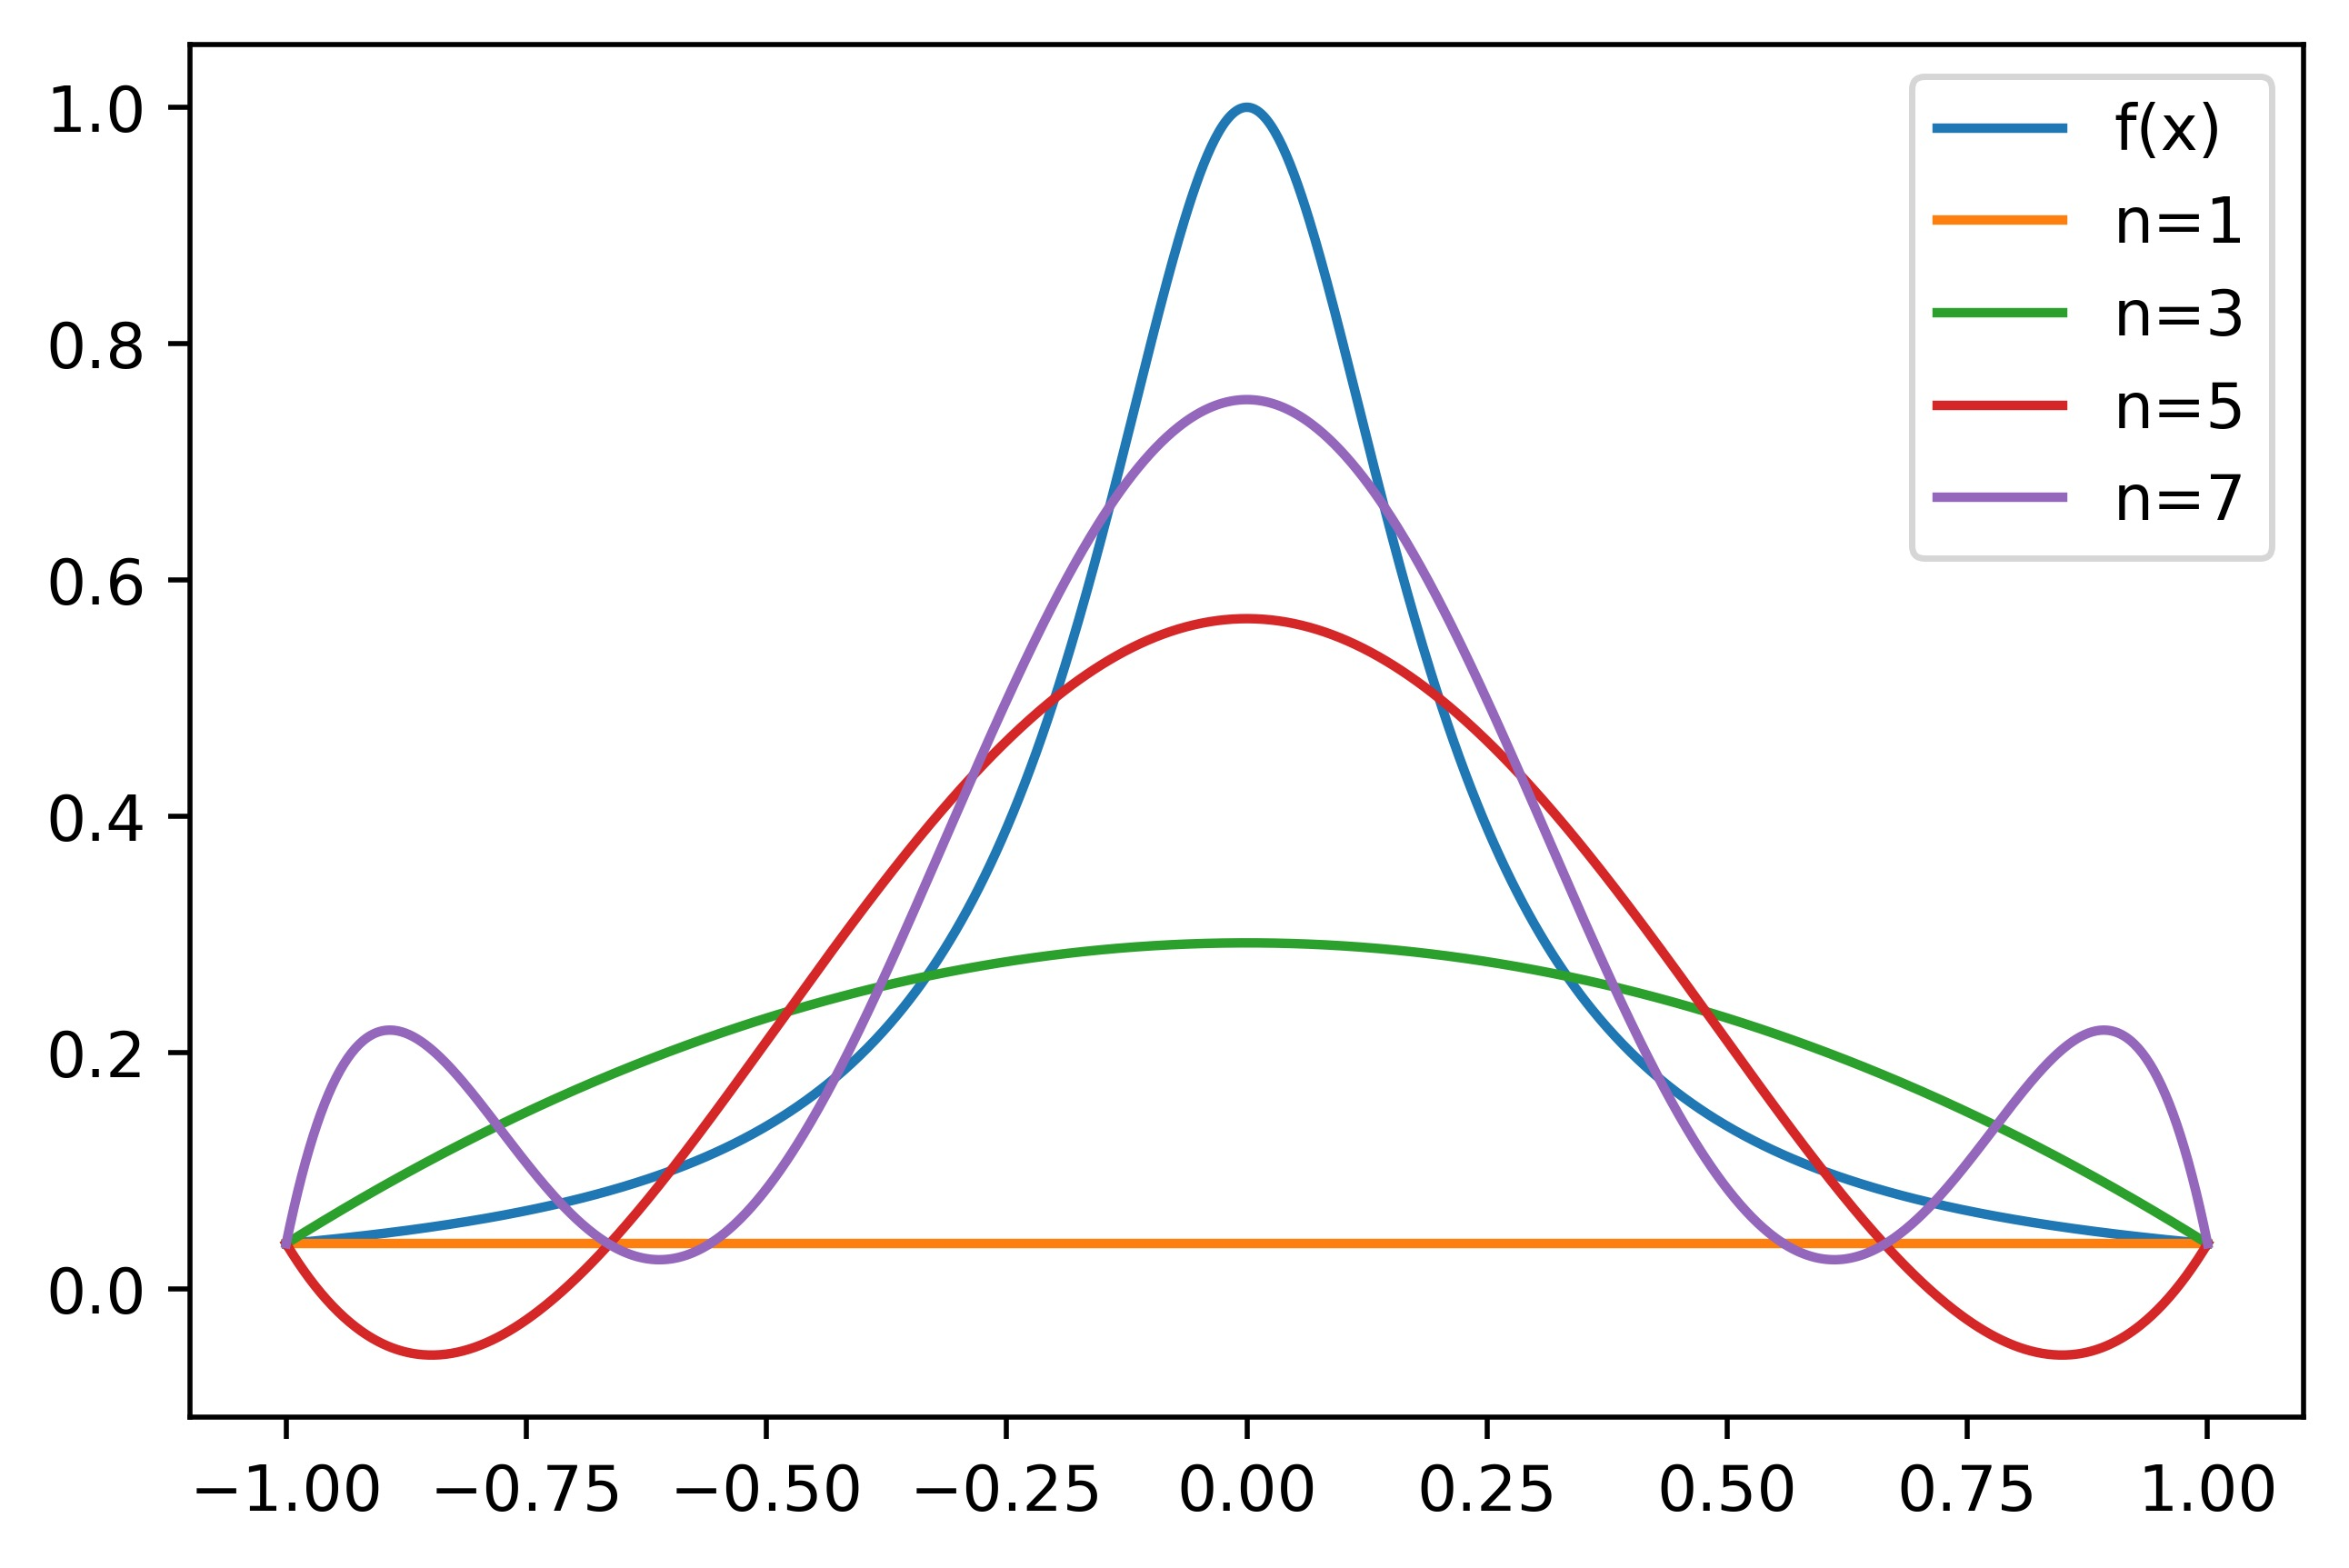
\includegraphics[scale=0.1]{6DL/pic/Runge.jpeg}
		\caption{Runge's phenomenon: Runge function $f(x)=\frac{1}{1+25x^{2}}$ and its polynomial interpolation $p_n(x)$.}
	\end{center}
\end{figure}

The experiment shows that  the polynomials $p_n(x)$ produced in this manner may in fact diverge away from $f(x)$ as $n$ increases. This typically occurs in an oscillating pattern that magnifies near the ends of the interpolation points. This phenomenon is attributed to Runge.

Thus, this particular set of polynomial functions $p_n(x)$ is not guaranteed to have the property of uniform convergence. In other words, Weierstrass' theorem guarantees the existence of the polynomial functions, but how to find such polynomials is not provided.

\section{Fourier transform and Fourier series}
We make use of the theory of tempered distributions (see
\cite{strichartz2003guide} for an introduction)
and we begin by collecting some results of independent interest, which
will also be important later. 
\subsection{Fourier transform}
Before studying the Fourier transform, we first consider Schwartz space which is defined below.
\begin{definition} \label{def:schwarz}
The Schwartz space $\mathcal{S}\left(\mathbb{R}^{n}\right)$ is the topological vector space of functions $f: \mathbb{R}^{n} \rightarrow \mathbb{C}$ such that $f \in C^{\infty}\left(\mathbb{R}^{n}\right)$ and
$$
x^{\alpha} \partial^{\beta} f(x) \rightarrow 0 \quad \text { as }|x| \rightarrow \infty
$$
for every pair of multi-indices $\alpha, \beta \in \mathbb{N}_{0}^{n} .$ For $\alpha, \beta \in \mathbb{N}_{0}^{n}$ and $f \in \mathcal{S}\left(\mathbb{R}^{n}\right)$ let
(5.10)
$$
\|f\|_{\alpha, \beta}=\sup _{\mathbb{R}^{n}}\left|x^{\alpha} \partial^{\beta} f\right|
$$
A sequence of functions $\left\{f_{k}: k \in \mathbb{N}\right\}$ converges to a function $f$ in $\mathcal{S}\left(\mathbb{R}^{n}\right)$ if
$$
\left\|f_{n}-f\right\|_{\alpha, \beta} \rightarrow 0 \quad \text { as } k \rightarrow \infty
$$
for every $\alpha, \beta \in \mathbb{N}_{0}^{n}$.
\end{definition}
The Schwartz space consists of smooth functions whose derivatives and the function itself decay at infinity faster than any power. Schwartz functions are rapidly decreasing. When there is no ambiguity, we will write $\mathcal{S}\left(\mathbb{R}^{n}\right)$ as $\mathcal{S}$.
Roughly speaking, tempered distributions grow no faster than a polynomial at infinity.

\begin{definition}
A tempered distribution $T$ on $\mathbb{R}^{n}$ is a continuous linear functional $T: \mathcal{S}\left(\mathbb{R}^{n}\right) \rightarrow \mathbb{C} .$ The topological vector space of tempered distributions is denoted by $\mathcal{S}^{\prime}\left(\mathbb{R}^{n}\right)$ or $\mathcal{S}^{\prime} .$ If $\langle T, f\rangle$ denotes the value of $T \in \mathcal{S}^{\prime}$ acting on $f \in \mathcal{S}$
then a sequence $\left\{T_{k}\right\}$ converges to $T$ in $\mathcal{S}^{\prime}$, written $T_{k} \rightarrow T$, if
$$
\left\langle T_{k}, f\right\rangle \rightarrow\langle T, f\rangle
$$
for every $f \in \mathcal{S}$.
\end{definition}
Since $\mathcal{D} \subset \mathcal{S}$ is densely and continuously imbedded, we have $\mathcal{S}^{\prime} \subset \mathcal{D}^{\prime} .$ Moreover, a distribution $T \in \mathcal{D}^{\prime}$ extends uniquely to a tempered distribution $T \in \mathcal{S}^{\prime}$ if and only if it is continuous on $\mathcal{D}$ with respect to the topology on $\mathcal{S}$. Every function $f \in L_{\text {loc }}^{1}$ defines a regular distribution $T_{f} \in \mathcal{D}^{\prime}$ by
$$
\left\langle T_{f}, \phi\right\rangle=\int f \phi d x \quad \text { for all } \phi \in \mathcal{D}.
$$
If $|f| \leq p$ is bounded by some polynomial $p,$ then $T_{f}$ extends to a tempered distribution $T_{f} \in \mathcal{S}^{\prime}$, but this is not the case for functions $f$ that grow too rapidly at infinity.

The Schwartz space is a natural one to use for the Fourier transform. Differentiation and multiplication exchange roles under the Fourier transform and therefore so do the properties of smoothness and rapid decrease. As a result, the Fourier transform is an automorphism of the Schwartz space. By duality, the Fourier transform is also an automorphism of the space of tempered distributions.

\begin{definition}\label{def:fourier1}
The Fourier transform of a function $f \in \mathcal{S}\left(\mathbb{R}^{n}\right)$ is the function $\hat{f}: \mathbb{R}^{n} \rightarrow \mathbb{C}$ defined by 
$$
\hat{f}(\omega)= \int f(x) e^{-2 \pi i\omega \cdot x} d x.
$$
The inverse Fourier transform of $f$ is the function $\check{f}: \mathbb{R}^{n} \rightarrow \mathbb{C}$ defined by
$$
\check{f}(x)=\int f(\omega) e^{2 \pi i\omega \cdot x} d k.
$$
\end{definition}

\begin{definition}\label{def:fourier2}
The Fourier transform of a tempered distribution $f \in \mathcal{S}'$ is  defined by 
$$
\langle \hat{f}, \phi\rangle = \langle f, \hat \phi\rangle,\quad \forall \phi\in \mathcal{S}.
$$ 
\end{definition}

The support of a continuous function $f$ is the closure  of the set $\{x\in \mathbb{R}: f(x)\neq 0\}$.
\begin{properties}
The Fourier transform has the following properties
\begin{enumerate}
\item If $f\in \mathcal{S}'$ and the support of $\hat f$ is $\{0\}$, then $f$ is a polynomial.
\item If $f\in \mathcal{S}'$ and the support of $\hat f$ is a single point $\{a\}$, then $f(x)=e^{2\pi iax}P(x)$, where $P(x)$ is a polynomial.
\end{enumerate}
\end{properties}







\subsection{Poisson summation formula}
\input{6DL/PoissonSum}
\subsection{A special cut-off function}
\input{6DL/Cut-off-function}

\subsection{Fourier transform of polynomials}
We begin by noting that an activation
function $\sigma$, which satisfies a polynomial growth condition
$|\sigma(x)| \leq C(1 + |x|)^n$ for some constants $C$ and $n$, is a
tempered distribution. As a result, we make this assumption on our
activation functions in the following theorems. We briefly note that
this condition is sufficient, but not necessary (for instance an
integrable function need not satisfy a pointwise polynomial growth
bound) for $\sigma$ to be represent a tempered distribution.

 We begin by studying the convolution of $\sigma$ with a Gaussian mollifier. Let $\eta$ be a Gaussian mollifier
 \begin{equation}
  \eta(x) = \frac{1}{\sqrt{\pi}}e^{-x^2}.
 \end{equation}
Set $\eta_\epsilon=\frac{1}{\epsilon}\eta(\frac{x}{\epsilon})$. Then consider 
\begin{equation}
\label{sigma-epsilon}
\sigma_{\epsilon}(x):=\sigma\ast{\eta_\epsilon}(x)=\int_{\mathbb{R}}\sigma(x-y){\eta_\epsilon}(y)dy
\end{equation}
for a given activation function $\sigma$.
It is clear that $\sigma_{\epsilon}\in C^\infty(\mathbb{R})$. Moreover, by considering the Fourier transform (as a tempered
distribution) we see that
\begin{equation}\label{eq_278}
 \hat{\sigma}_{\epsilon} = \hat{\sigma}\hat{\eta}_{\epsilon} = \hat{\sigma}\eta_{\epsilon^{-1}}.
\end{equation} 


We begin by stating a lemma which characterizes the set of polynomials in terms of their
 Fourier transform.
\begin{lemma}\label{polynomial_lemma} Given a tempered distribution
  $\sigma$,  the following statements are equivalent:
\begin{enumerate}
\item $\sigma$ is a polynomial 
\item $\sigma_\epsilon$ given by \eqref{sigma-epsilon} is a polynomial for any
  $\epsilon>0$. 
\item $\text{\normalfont supp}(\hat{\sigma})\subset \{0\}$. 
\end{enumerate}
\end{lemma}
\begin{proof}
  We begin by proving that (3) and (1) are equivalent.  This follows
  from a characterization of distributions supported at a single point
  (see \cite{strichartz2003guide}, section 6.3). In particular, a
  distribution supported at $0$ must be a finite linear combination of
  Dirac masses and their derivatives.  In particular, if
  $\hat{\sigma}$ is supported at $0$, then
  \begin{equation}
   \hat{\sigma} = \displaystyle\sum_{i=1}^n a_i\delta^{(i)}.
  \end{equation}
  Taking the inverse Fourier transform and noting that the inverse
  Fourier transform of $\delta^{(i)}$ is $c_ix^i$, we see that
  $\sigma$ is a polynomial. This shows that (3) implies (1), for the
  converse we simply take the Fourier transform of a polynomial and
  note that it is a finite linear combination of Dirac masses and
  their derivatives.
  
  Finally, we prove the equivalence of (2) and (3). For this it
  suffices to show that $\hat{\sigma}$ is supported at $0$ iff
  $\hat{\sigma}_\epsilon$ is supported at $0$. This follows from
  equation \ref{eq_278} and the fact that $\eta_{\epsilon^{-1}}$ is
  nowhere vanishing.
\end{proof}

As an application of Lemma \ref{polynomial_lemma}, we give a
simple proof of the result in the next section.   


\section{Qualitative approximation of neural networks}
The first question about ${\rm DNN}_1$ is about the approximation
properties for any continuous functions. Here we have the next
theorem. 

The first proof for this theorem above can be found in
\cite{leshno1993multilayer} and summarized in
\cite{pinkus1999approximation}.  %The next theorem plays an important role in the proof of above lemma, which is first proved in \cite{leshno1993multilayer} with several steps. 
Here we can present a
more direct and simple version.


\begin{theorem}[Universal Approximation Property of Shallow Neural
 Networks]
 Let $\sigma$ be a Riemann integrable function and $\sigma\in
 L_{loc}^\infty(\mathbb{R})$.  Then $\Sigma_d(\sigma)$ 
 in dense in
 $C(\Omega)$ for any compact $\Omega\subset \mathbb{R}^n$ if and and
 only if $\sigma$ is not a polynomial!

Namely, if $\sigma$ is not a polynomial,  then, for  any $f\in C(\bar \Omega)$,
 there exists a sequence $\phi_n \in {\rm DNN}_1$ such that
$$
	\max_{x\in \bar \Omega} |\phi_n(x) - f(x)| \to 0, \quad n \to \infty.
$$
\end{theorem}

\begin{proof}
Let us first prove the theorem in a special case that $\sigma\in
C^\infty(\mathbb{R})$.
Since $\sigma\in C^\infty(\mathbb{R})$, it follows that for every $\omega,b$,
\begin{equation}
 \frac{\partial}{\partial \omega_j}\sigma(\omega\cdot x+b) = 
 \lim_{n\rightarrow \infty}\frac{\sigma((\omega+h e_j)\cdot x+b)-\sigma(\omega\cdot x+b)}{h} \in \overline{\Sigma}_d(\sigma)
\end{equation}
for all $j=1,...,d$. 

By the same argument, for $\alpha = (\alpha_1,...,\alpha_d)$
$$D^\alpha_\omega\sigma(\omega\cdot x+b)\in\overline{\Sigma}_d(\sigma)$$
for all $k\in\mathbb{N}$, $j=1,...,d$, $\omega\in\mathbb{R}^d$ and $b\in\mathbb{R}$.

Now 
$$
D^\alpha_\omega\sigma(\omega\cdot x+b)=x^\alpha\sigma^{(k)}(\omega\cdot x+b)
$$
where $k=|\alpha|$ and $x^\alpha = x_1^{\alpha_1}\cdots x_d^{\alpha_d}$.  Since
$\sigma$ is not a polynomial there exists a $\theta_k\in\mathbb{R}$
such that $\sigma^{(k)}(\theta_k)\ne0$.  Taking $\omega=0$ and
$b=\theta_k$, we thus see that $x_j^k\in\overline{\Sigma}_d(\sigma)$.
Thus, all polynomials of the form $x_1^{k_1}\cdots x_d^{k_d}$ are in
$\overline{\Sigma}_d(\sigma)$.

This implies that $\overline{\Sigma}_d(\sigma)$ contains all
polynomials.  By Weierstrass's Theorem \cite{stone1948generalized} it
follows that $\overline{\Sigma}_d(\sigma)$ contains $C(K)$ for each
compact $K\subset\mathbb{R}^n$. That is $\Sigma_d(\sigma)$ is dense in
$C(\mathbb{R}^d)$.

Now we consider the case that $\sigma$ is only Riemann integrable. 
Consider the mollifier $\eta$
	\begin{equation*}
	\begin{aligned}
	\eta(x)=\frac{1}{\sqrt {\pi}}e^{-x^2}.
	\end{aligned}
	\end{equation*}
Set $\eta_\epsilon=\frac{1}{\epsilon}\eta(\frac{x}{\epsilon})$. Then consider $\sigma_{\eta_\epsilon}$
\begin{equation}
\sigma_{\eta_\epsilon}(x):=\sigma\ast{\eta_\epsilon}(x)=\int_{\mathbb{R}}\sigma(x-y){\eta_\epsilon}(y)dy
\end{equation}
It can be seen that $\sigma_{\eta_\epsilon}\in C^\infty(\mathbb{R})$.
We first notice that
$\overline{\Sigma}_1(\sigma_{\eta_\epsilon})\subset\overline{\Sigma}_1(\sigma)$,
which can be done easily by checking the Riemann sum of
$\sigma_{\eta_\epsilon}(x)=\int_{\mathbb{R}}\sigma(x-y){\eta_\epsilon}(y)dy$
is in $\overline{\Sigma}_1(\sigma)$.

Following the argument in the beginning of the proof proposition, we
want to show that $\overline{\Sigma}_1(\sigma_{\eta_\epsilon}))$
contains all polynomials.  For this purpose, it suffices to show that
there exists $\theta_k$ and $\sigma_{\eta_\epsilon}$ such that
$\sigma_{\eta_\epsilon}^{(k)}(\theta_k)\ne0$ for each k. If not, then
there must be $k_0$ such that
$\sigma_{\eta_\epsilon}^{(k_0)}(\theta)=0$ for all
$\theta\in\mathbb{R}$ and all $\epsilon>0$.  Thus
$\sigma_{\eta_\epsilon}$'s are all polynomials with degree at most
$k_0-1$.  In particular, It is known that $\eta_\epsilon\in
C_0^\infty(\mathbb{R})$ and $\sigma\ast\eta_\epsilon$ uniformly
converges to $\sigma$ on compact sets in $\mathbb{R}$ and
$\sigma\ast\eta_\epsilon$'s are all polynomials of degree at most
$k_0-1$. Polynomials of a fixed degree form a closed linear subspace,
therefore $\sigma$ is also a polynomial of degree at most $k_0-1$,
which leads to contradiction.
\end{proof}

%\subsection{Fourier transform of polynomials}
We begin by noting that an activation
function $\sigma$, which satisfies a polynomial growth condition
$|\sigma(x)| \leq C(1 + |x|)^n$ for some constants $C$ and $n$, is a
tempered distribution. As a result, we make this assumption on our
activation functions in the following theorems. We briefly note that
this condition is sufficient, but not necessary (for instance an
integrable function need not satisfy a pointwise polynomial growth
bound) for $\sigma$ to be represent a tempered distribution.

 We begin by studying the convolution of $\sigma$ with a Gaussian mollifier. Let $\eta$ be a Gaussian mollifier
 \begin{equation}
  \eta(x) = \frac{1}{\sqrt{\pi}}e^{-x^2}.
 \end{equation}
Set $\eta_\epsilon=\frac{1}{\epsilon}\eta(\frac{x}{\epsilon})$. Then consider 
\begin{equation}
\label{sigma-epsilon}
\sigma_{\epsilon}(x):=\sigma\ast{\eta_\epsilon}(x)=\int_{\mathbb{R}}\sigma(x-y){\eta_\epsilon}(y)dy
\end{equation}
for a given activation function $\sigma$.
It is clear that $\sigma_{\epsilon}\in C^\infty(\mathbb{R})$. Moreover, by considering the Fourier transform (as a tempered
distribution) we see that
\begin{equation}\label{eq_278}
 \hat{\sigma}_{\epsilon} = \hat{\sigma}\hat{\eta}_{\epsilon} = \hat{\sigma}\eta_{\epsilon^{-1}}.
\end{equation} 


We begin by stating a lemma which characterizes the set of polynomials in terms of their
 Fourier transform.
\begin{lemma}\label{polynomial_lemma} Given a tempered distribution
  $\sigma$,  the following statements are equivalent:
\begin{enumerate}
\item $\sigma$ is a polynomial 
\item $\sigma_\epsilon$ given by \eqref{sigma-epsilon} is a polynomial for any
  $\epsilon>0$. 
\item $\text{\normalfont supp}(\hat{\sigma})\subset \{0\}$. 
\end{enumerate}
\end{lemma}
\begin{proof}
  We begin by proving that (3) and (1) are equivalent.  This follows
  from a characterization of distributions supported at a single point
  (see \cite{strichartz2003guide}, section 6.3). In particular, a
  distribution supported at $0$ must be a finite linear combination of
  Dirac masses and their derivatives.  In particular, if
  $\hat{\sigma}$ is supported at $0$, then
  \begin{equation}
   \hat{\sigma} = \displaystyle\sum_{i=1}^n a_i\delta^{(i)}.
  \end{equation}
  Taking the inverse Fourier transform and noting that the inverse
  Fourier transform of $\delta^{(i)}$ is $c_ix^i$, we see that
  $\sigma$ is a polynomial. This shows that (3) implies (1), for the
  converse we simply take the Fourier transform of a polynomial and
  note that it is a finite linear combination of Dirac masses and
  their derivatives.
  
  Finally, we prove the equivalence of (2) and (3). For this it
  suffices to show that $\hat{\sigma}$ is supported at $0$ iff
  $\hat{\sigma}_\epsilon$ is supported at $0$. This follows from
  equation \ref{eq_278} and the fact that $\eta_{\epsilon^{-1}}$ is
  nowhere vanishing.
\end{proof}

As an application of Lemma \ref{polynomial_lemma}, we give a
simple proof of the result in the next section.   
  % this is actually for
%quantitative/asymptotic analysis
\section{Asymptotic approximation properties}
\subsection{Monte Carlo sampling and analysis}
\input{6DL/EEn}

\begin{lemma}   \label{MC}
For any $g\in L^\infty(G)$, we have
  \begin{equation}
  \begin{split}
    \mathbb{E}_n\Big(\mathbb{E}g-\frac1n\sum_{i=1}^n
    g(\omega_i)\Big)^2
    &=\frac{1}{n}\mathbb{V}(g)=\frac{1}{n}\Big(\mathbb{E}(g^2) - \big (\mathbb{E}(g)\big )^2\Big)
    \\
    &=
    \left\{
             \begin{aligned}
    \frac{1}{n}\mathbb{V}(g)
   & \le\frac{1}{n} \sup_{\omega, \omega'\in G} |g(\omega) - g(\omega')|^2
    \\
\frac{1}{n}\Big(\mathbb{E}(g^2) - \big (\mathbb{E}(g)\big )^2\Big)
&\le\frac{1}{n} \mathbb E(g^2)\le \frac{1}{n}\|g\|^2_{L^\infty},
\end{aligned}
\right.
\end{split}
  \end{equation} 
\end{lemma}

\begin{proof}%[Proof of Lemma \ref{MC}]
First note that
 \begin{equation}
    \label{eqn}
    \begin{aligned}
\left(\mathbb{E} g-\frac1N\sum_{i=1}^Ng(\omega_i)\right)^2 
  & 
=\frac{1}{N^2} \left(\sum_{i=1}^N(\mathbb{E} g-g(\omega_i))\right)^2 
  \\
  &=\frac{1}{N^2} \sum_{i,j=1}^N(\mathbb{E} g-g(\omega_i))(\mathbb{E} g-g(\omega_j))
  \\
  &=\frac{I_1}{N^2} +\frac{I_2}{N^2}.
    \end{aligned}
  \end{equation}
with 
\begin{equation}
I_1= \sum_{i=1}^N(\mathbb{E} g-g(\omega_i))^2,\quad I_2=\sum_{i\neq  j}^N\left ((\mathbb{E}g)^2-\mathbb {E}(g)(g(\omega_i)+
g(\omega_j))+g(\omega_i)g(\omega_j))\right).
\end{equation}
Consider $I_1$, for any $i$,
 $$
 \mathbb{E}_N(\mathbb{E} g-g(\omega_i))^2
 =\mathbb{E}(\mathbb{E} g-g)^2 = \mathbb{V}(g).
 $$ 
Thus,
$$
 \mathbb{E}_N (I_1) = n\mathbb{V}(g).
$$
For $I_2$, note that
$$
\mathbb E_N g(\omega_i)=\mathbb E_N g(\omega_j) =\mathbb E(g)
$$
and, for $i\neq j$,
\begin{equation}\label{key}
\begin{aligned}
\mathbb {E}_N ( g(\omega_i)g(\omega_j)) &= 
\int_{G\times G\times\ldots\times G}
g(\omega_i) g(\omega_j) \lambda(\omega_1) \lambda(\omega_2)\ldots \lambda(\omega_N)
d\omega_1d\omega_2\cdots d\omega_N \\
&= \int_{G\times G} g(\omega_i) g(\omega_j) \lambda(\omega_1) 
\lambda(\omega_1) \lambda(\omega_2)
d\omega_1d\omega_2 \\
&= \mathbb {E}_N (
g(\omega_i))\mathbb {E}_n(g(\omega_j))
=[\mathbb E(g)]^2.
\end{aligned}
\end{equation}
Thus
 \begin{equation}
\mathbb{E}_N (I_2) = \mathbb{E}_N \left( \sum_{i\neq j}^N((\mathbb{E}g)^2-\mathbb
  E(g)(\mathbb E(g(\omega_i))+ \mathbb E(g(\omega_j)))+\mathbb E(g(\omega_i)g(\omega_j))) \right)=0.
  \end{equation}
Consequently, there exist the following two formulas for $\displaystyle \mathbb{E}_N\left(\mathbb{E} g-
      \frac1N\sum_{i=1}^Ng(\omega_i)\right)^2$:
 \begin{equation} 
 \mathbb{E}_N\left(\mathbb{E} g-
      \frac1N\sum_{i=1}^Ng(\omega_i)\right)^2 = \frac{1}{N^2}\mathbb{E}_N (I_1)
      =
           \left\{
             \begin{aligned}
            \frac{1}{N}\mathbb{E}\big ((\mathbb{E} g-g)^2\big )\\
            \frac{1}{N}(\mathbb{E}(g^2) - (\mathbb{E} g)^2).
            \end{aligned}
    \right.
  \end{equation}
Based on the first formula above, since
$$
|g(\omega) - \mathbb{E} g|=|\int_G \big (g(\omega) - g(\tilde \omega) \big )\lambda(\tilde \omega)d\tilde \omega|\le \sup_{\omega, \omega'\in G} |g(\omega) - g(\omega')|,
$$
it holds that
 \begin{equation} 
 \mathbb{E}_N\left(\mathbb{E} g-
      {1\over N }\sum_{i=1}^Ng(\omega_i)\right)^2 
            \le\frac{1}{N} \sup_{\omega, \omega\in G} |g(\omega) - g(\omega')|^2.
  \end{equation}
Due to the second formula above,  
 \begin{equation}
    \label{eqn}
 \mathbb{E}_N\left(\mathbb{E} g-
      \frac1N\sum_{i=1}^Ng(\omega_i)\right)^2  
            \le\frac{1}{N} \mathbb E(g^2)\le\frac{1}{N}\|g\|^2_{L^\infty}
  \end{equation}
which completes the proof.
\end{proof}

We can also generalize Lemma \ref{MC} to Hilbert spaces following a similar analysis.

\begin{lemma}    
For any $g: G\rightarrow H$ where $H$ is a Hilbert space, we have
  \begin{equation}
  \begin{split}
    \mathbb{E}_n\Big(\|\mathbb{E}g-\frac1n\sum_{i=1}^n
    g(\omega_i)\|_H^2\Big)
    &=\frac{1}{n}\mathbb{V}(g)=\frac{1}{n}\Big(\mathbb{E}(\|g\|_H^2) - \big (\mathbb{E}(\|g\|_H)\big )^2\Big)
    \\
    &=
    \left\{
             \begin{aligned}
    \frac{1}{n}\mathbb{V}(g)
   & \le\frac{1}{n} \sup_{\omega, \omega'\in G} \|g(\omega) - g(\omega')\|_H^2
    \\
\frac{1}{n}\Big(\mathbb{E}(\|g\|_H^2) - \big (\mathbb{E}(\|g\|_H)\big )^2\Big)
&\le\frac{1}{n} \mathbb E(\|g\|_H^2),
\end{aligned}
\right.
\end{split}
  \end{equation} 
\end{lemma}

\begin{proof}%[Proof of Lemma \ref{MC}]
First note that
 \begin{equation}
    \label{eqn}
    \begin{aligned}
\left\|\mathbb{E} g-\frac1N\sum_{i=1}^Ng(\omega_i)\right\|_H^2 
  & 
=\frac{1}{N^2} \left\|\sum_{i=1}^N(\mathbb{E} g-g(\omega_i))\right\|_H^2 
  \\
  &=\frac{1}{N^2} \sum_{i,j=1}^N\left(\mathbb{E} g-g(\omega_i), \mathbb{E} g-g(\omega_j)\right)
  \\
  &=\frac{I_1}{N^2} +\frac{I_2}{N^2}.
    \end{aligned}
  \end{equation}
with 
\begin{equation}
I_1= \sum_{i=1}^N\|\mathbb{E} g-g(\omega_i)\|_H^2,\quad I_2=\sum_{i\neq  j}^N\left(\mathbb{E} g-g(\omega_i), \mathbb{E} g-g(\omega_j)\right).
\end{equation}
Consider $I_1$, for any $i$,
 $$
 \mathbb{E}_N(\|\mathbb{E} g-g(\omega_i)\|_H^2)
 =\mathbb{E}(\|\mathbb{E} g-g\|_H^2) = \mathbb{V}(g).
 $$ 
Thus,
$$
 \mathbb{E}_N (I_1) = n\mathbb{V}(g).
$$
For $I_2$, note that
$$
\mathbb E_N \|g(\omega_i)\|_H=\mathbb E_N \|g(\omega_j)\|_H =\mathbb E(\|g\|_H)
$$
and, for $i\neq j$,
\begin{equation}\label{key}
\begin{aligned}
\mathbb {E}_N ( g(\omega_i), g(\omega_j)) &= 
\int_{G\times G\times\ldots\times G}
g(\omega_j) g(\omega_j) \lambda(\omega_1) \lambda(\omega_2)\ldots \lambda(\omega_N)
d\omega_1d\omega_2\cdots d\omega_N \\
&= \int_{G\times G} (g(\omega_j) , g(\omega_j) ) 
\lambda(\omega_i) \lambda(\omega_j)
d\omega_id\omega_j \\
&=\left( \mathbb {E}_N (
g(\omega)) , \mathbb {E}_N(g(\omega))\right)
=\|\mathbb E(g)\|_H^2.
\end{aligned}
\end{equation}
Thus
 \begin{equation}
\mathbb{E}_N (I_2) = \mathbb{E}_N \left( \sum_{i\neq j}^N\big(\|\mathbb{E}g\|_H^2-
(\mathbb  E(g), \mathbb E(g(\omega_i))+ \mathbb E(g(\omega_j)))
+ (g(\omega_i), g(\omega_j))\big) \right)=0.
  \end{equation}
Consequently, there exist the following two formulas for $\displaystyle \mathbb{E}_N\left\|\mathbb{E} g-
      \frac1N\sum_{i=1}^Ng(\omega_i)\right\|_H^2$:
 \begin{equation} 
 \mathbb{E}_N\left\|\mathbb{E} g-
      \frac1N\sum_{i=1}^Ng(\omega_i)\right\|_H^2 = \frac{1}{N^2}\mathbb{E}_N (I_1)
      =
           \left\{
             \begin{aligned}
            \frac{1}{N}\mathbb{E}\big (\|\mathbb{E} g-g\|_H^2\big )\\
            \frac{1}{N}(\mathbb{E}(\|g\|_H^2) - \|\mathbb{E} g\|_H^2).
            \end{aligned}
    \right.
  \end{equation}
Based on the first formula above, since
$$
|g(\omega) - \mathbb{E} g|=|\int_G \big (g(\omega) - g(\tilde \omega) \big )\lambda(\tilde \omega)d\tilde \omega|\le \sup_{\omega, \omega'\in G} |g(\omega) - g(\omega')|,
$$
it holds that
 \begin{equation} 
 \mathbb{E}_N\left\|\mathbb{E} g-
      {1\over N }\sum_{i=1}^Ng(\omega_i)\right\|_H^2 
            \le\frac{1}{N} \sup_{\omega, \omega'\in G} \|g(\omega) - g(\omega')\|_H^2.
  \end{equation}
Due to the second formula above,  
 \begin{equation}
    \label{eqn}
 \mathbb{E}_N\left\|\mathbb{E} g-
      \frac1N\sum_{i=1}^Ng(\omega_i)\right\|_H^2  
            \le\frac{1}{N} \mathbb E(\|g\|_H^2),
  \end{equation}
which completes the proof.
\end{proof}


%\input{6DL/MonteCarloProbability}
\begin{lemma}\label{lem:sample}
\textup{[Monte Carlo Sampling]}
	Consider 
	\begin{equation}
	\label{uv}
	u(x)=\int_{G}g(x,\theta)\rho(\theta)d\theta   = \mathbb E (g)
	\end{equation}
	with $0\le \rho(\theta)\in L^1(G)$. For any $N\ge 1$, there exist $\theta_i^*\in G$ such that
	$$
	\|u-u_N\|_{L^2(\Omega)}^2 
	\le\frac{1}{N}
	\int_G \|g(\cdot,\theta)\|_{L^2(\Omega)}^2\rho(\theta)d\theta = {\|\rho\|_{L^1(G)}\over N}\mathbb E (\|g(\cdot,\theta)\|_{L^2(\Omega)}^2)
	$$
	where  
	$
	\|g(\cdot,\theta)\|_{L^2(\Omega)}^2 = \int_{\Omega} [g(x,\theta)]^2 d\mu(x),
	$
	\begin{equation}\label{fndef} 
	u_N(x)=\frac{\|\rho\|_{L^1(G)}}{N}\sum_{i=1}^N g(x,\theta_i^*).
	\end{equation}

Similarly, if $g(\cdot, \theta)\in H^m(\Omega)$, for any $N\ge 1$, there exist $\theta_i^*\in G_i$ with $f_N$ given in \eqref{fndef} such that
	\begin{equation}\label{eq:hm}
	\|u-u_N\|_{H^m(\Omega)}^2 
	\le 
	\int_G  \|g(\cdot,\theta)\|_{H^m(\Omega)}^2\rho(\theta)d\theta
	=\frac{\|\rho\|_{L^1(G)}}{N} \mathbb E (\|g(\cdot,\theta)\|_{H^m(\Omega)}^2).
	\end{equation}
\end{lemma}

\iffalse
\begin{proof} 
Note that
\begin{equation}
\label{uv}
u(x) = \|\rho\|_{L^1(G)}\mathbb E (g).
\end{equation}
By Lemma \ref{MC},
$$
\mathbb {E}_n\left(\bigg(\mathbb E(g(x,\cdot))
-\frac{1}{N}\sum_{i=1}^N g(x,\theta_i))\bigg)^2
\right)\le {1\over N} \mathbb E (g^2).
$$
By taking integration w.r.t. $x$ on both sides, we get
$$
\mathbb {E}_n\left(h(\theta_1,\theta_2, \cdots, \theta_N)
\right)\le {1\over N} \mathbb {E} \Big(\int_{\Omega} g^2 d\mu(x)\Big),
$$
where 
$$
h(\theta_1,\theta_2, \cdots, \theta_N) =  \int_{\Omega} \bigg(\mathbb E(g(x,\cdot))
-\frac{1}{N}\sum_{i=1}^N g(x,\theta_i))\bigg)^2 d\mu(x).
$$
Since $\mathbb {E}_N (1) = 1$ and $\mathbb {E}_N (h) \le {1\over N} \mathbb {E} \Big(\int_{\Omega} g^2 d\mu(x)\Big)$, there exist $\theta_i^* \in G$ such that
$$
h(\theta_1^*, \theta_2^*, \cdots, \theta_N^*) \le  {1\over N}  \int_{\Omega} \mathbb {E} (g^2) d\mu(x).
$$
%Otherwise, $\mathbb {E}_n\left(h \right) >  {1\over n} \mathbb {E} \Big(\int_{\Omega} g^2 d\mu(x)\Big)$   if $h(\theta_1,\theta_2, \cdots, \theta_n) > {1\over n}  \int_{\Omega} \mathbb {E} (g^2)) d\mu(x)$. 
This implies that
$$
	\mathbb{E}_n\|u-u_N\|_{L^2(\Omega)}^2 
	\le\frac{\|\rho\|_{L^1(G)}}{N}
	\int_G \|g(\cdot,\theta)\|_{L^2(\Omega)}^2\lambda(\theta)d\theta.
	$$ 
	The proof for \eqref{eq:hm} is similar to the above analysis for the $L^2$-error analysis, which completes the proof.
\end{proof}
\fi



We also have a more general version of the above lemma.
\begin{lemma}\label{lem:sampleHk}
	Let 
	\begin{equation} \label{uint}
	u(x)=\int_{G}g(x,\theta)\lambda(\theta)d\theta  = \mathbb E (g)
	\end{equation}
	with $\|\lambda(\theta)\|_{L^1(\Theta)}=1$.
	For any $N\ge 1$, there exist $\theta_i^*\in G$ such that
	$$
	\|u-u_N\|_{H^m(\Omega)}^2 
	\le 
	\int_G  \|g(\cdot,\theta)\|_{H^m(\Omega)}^2\lambda(\theta)d\theta
	=\frac{1}{N} \mathbb E (\|g(\cdot,\theta)\|_{H^m(\Omega)}^2)
	$$
	where 
	$$
	u_N(x)=\frac{1}{N}\sum_{i=1}^N g(x,\theta_i^*)
	$$
	In particular, if 
	\begin{equation}
	\label{eq:4}
	|D^\alpha g(x,\theta)|\le C, \quad\forall x, \theta, |\alpha|\le m
	\end{equation}
	Then
	$$
	\|u-u_N\|_{H^m(\Omega)}
	\le 
	\begin{pmatrix}
	m+d\\
	m
	\end{pmatrix}^{1/2}
	|\Omega|^{1/2}
	N^{-1/2}.
	$$
\end{lemma}

\subsection{Stratified sampling and analysis}
Stratified sampling  \cite{bickel1984asymptotic} gives a more refined version of the Monte Carlo method. 

\begin{lemma} \label{lem:stratified}
 For any
  nonoverlaping decomposition $G=G_1\cup G_2\cup \cdots \cup G_M$ and
  positive integer $n$, let $n_i=\lceil \lambda(G_i)n\rceil$ be the smallest integer larger than $\lambda(G_i)n$ and $\displaystyle N=\sum_{i=1}^M n_i$.  Let $\theta_{i,j}\in G_i (1\le j\le n_i)$ and 
\begin{equation}
g_n=\sum_{i=1}^M \lambda(G_i)g_{n_i}^i \quad \mbox{with}\quad g_{n_i}^i={1 \over n_i}\sum_{j=1}^{n_i} g(\theta_{i,j}).
\end{equation} 
It holds that  
\begin{equation}
\mathbb{E}_N(\mathbb{E}_G g -g_N)^2=\sum_{i=1}^M {\lambda^2(G_i) \over n_i} \mathbb{E}_{G_i}\big (g -\mathbb{E}_{G_i}g\big )^2
\le {1 \over n} \max_{1\le i\le M}\sup_{\theta, \theta'\in G_i}\big |g(\theta) - g(\theta')\big |^2.
\end{equation}
\end{lemma} 

\begin{proof}%[Proof of Lemma \ref{lem:stratified}]
It follows from definition that
\begin{equation}
g(x, \theta) = \sum_{i=1}^M \lambda(G_i) g(x, \theta),\qquad \mathbb{E}_G g =\sum_{i=1}^M\lambda(G_i) \int_{G_i} g\lambda_i(\theta)d\theta = \sum_{i=1}^M \lambda(G_i) \mathbb{E}_{G_i}g.
\end{equation}
Thus, the difference $g - \mathbb{E}_G g$ is a linear combination of $g -\mathbb{E}_{G_i}g$ on each $G_i$ as follows
\begin{equation}
g - \mathbb{E}_G g = \sum_{i=1}^M \lambda(G_i) \big (g -\mathbb{E}_{G_i}g\big ).
\end{equation}
It follows from 
\begin{equation}
\mathbb{E}_G g-g_n=\sum_{i=1}^M \lambda(G_i) (\mathbb{E}_{G_i}g -  g^i_{ n_i})
\end{equation}
and \eqref{En} that
\begin{equation} 
\mathbb{E}_n(\mathbb{E}_G g -g_n)^2 =\sum_{i,j=1}^M \lambda(G_i) \lambda(G_j) \mathbb{E}_n \big ((\mathbb{E}_{G_i}g -  g^i_{ n_i})(\mathbb{E}_{G_j}g -  g^j_{ n_j})\big )
=\sum_{i,j=1}^M \lambda(G_i) \lambda(G_j) I_{ij}  
\end{equation}
with 
$$
I_{ij} = \mathbb{E}_n \big ((\mathbb{E}_{G_i}g -  g^i_{ n_i})(\mathbb{E}_{G_j}g -  g^j_{ n_j})\big ).
$$
\iffalse
If $i\neq j$,
\begin{equation}\label{eq:Iij}
\begin{split}
I_{ij}=&\int_{G\times \cdots\times G} (\mathbb{E}_{G_i}g -  g^i_{ n_i})(\mathbb{E}_{G_j}g -  g^j_{ n_j})\lambda(\theta_{i,n_1})\cdots\lambda(\theta_{i,n_i})\lambda(\theta_{j,1})\cdots \lambda(\theta_{j,n_j})d\theta_{i,1}\cdots d\theta_{i,n_i}d\theta_{j,1}\cdots d\theta_{j,n_j}
\\
=&\int_{G\times \cdots\times G} (\mathbb{E}_{G_i}g -  g^i_{ n_i})\lambda(\theta_{i,n_1})\cdots\lambda(\theta_{i,n_i})d\theta_{i,1}\cdots d\theta_{i,n_i}
\\
&+
\int_{G\times \cdots\times G} (\mathbb{E}_{G_i}g -  g^j_{ n_j})\lambda(\theta_{j,1})\cdots \lambda(\theta_{j,n_j})d\theta_{j,1}\cdots d\theta_{j,n_j}
\\
=&\lambda^{n_i}(G_i)\int_{G_i\times \cdots\times G_i} (\mathbb{E}_{G_i}g -  g^i_{ n_i})\lambda_i(\theta_{i,n_1})\cdots\lambda_i(\theta_{i,n_i})d\theta_{i,1}\cdots d\theta_{i,n_i}
\\
&+
\lambda^{n_j}(G_j)\int_{G\times \cdots\times G} (\mathbb{E}_{G_i}g -  g^j_{ n_j})\lambda_j(\theta_{j,1})\cdots \lambda_j(\theta_{j,n_j})d\theta_{j,1}\cdots d\theta_{j,n_j}
\\
=&0.
\end{split}
\end{equation}
\fi
By Lemma \ref{MC},
\begin{equation}
I_{ij} =  \mathbb{E}_n \big ((\mathbb{E}_{G_i}g -  g^i_{ n_i})^2\big )\delta_{ij}= {1\over n_i} \mathbb{E} \big ((\mathbb{E}_{G_i}g -  g)^2\big )\delta_{ij}.
\end{equation}
Thus,
\begin{equation} 
\mathbb{E}_n(\mathbb{E}_G g -g_n)^2 =\sum_{i=1}^M {\lambda^2(G_i) \over n_i} \mathbb{E}_{G_i}\big (g -\mathbb{E}_{G_i}g\big )^2, 
\end{equation}
which completes the proof.
\end{proof} 

Lemma \ref{MC} and Lemma \ref{lem:stratified} represent two simple identities and subsequent inequalities that can be verified by a direct calculation. Actually Lemma \ref{MC} is a special case of Lemma  \ref{lem:stratified} with $M=1$. Lemma \ref{MC} and Lemma \ref{lem:stratified} are the basis of Monte-Carlo sampling and  stratified sampling in statistics. 

\begin{lemma}\label{lem:stratifiedapprox}
\textup{[Stratified Sampling]}
	For $u(x)$ in \eqref{uint}
	with positive $\rho(\theta)\in L^1(G)$, given any positive integers $n$ and $M\le n$, for  any nonoverlaping decomposition $G=G_1\cup G_2\cup \cdots \cup G_M$, there exists$\{\theta_i^\ast\}_{i=1}^N$ with $n\le N \le 2n$ such that
	\begin{equation} 
	\|u - u_N\|_{L^2(\Omega)} \leq N^{-1/2}\|\rho\|_{L^1(G)}\max_{1\le j\le M}\sup_{\theta_{j},\theta_{j}'\in G_j} \| g(x,\theta_j) - g(x,\theta_j')\|_{L^2(\Omega)} 
	\end{equation}
	where 
	$$
	u_N(x)= {2\|\rho\|_{L^1(G)}\over N}\sum_{i=1}^N\beta_i g(x,\theta_i^\ast)
	$$ 
	and $\beta_i\in [0,1]$.
	\end{lemma}

\begin{proof}
Let $n_j=\lceil \lambda(G_j)n\rceil$ and $\theta_{i,j} \in G_j(1\leq i\leq n_j)$. Define $\displaystyle N=\sum_{j=1}^M n_j$ and
$$
u_N(x)=\|\rho\|_{L^1(G)}\sum_{i=1}^M \lambda(G_i)g_{n_i}^i \quad \mbox{with}\quad g_{n_i}^i={1 \over n_i}\sum_{j=1}^{n_i} g(\theta_{i,j}).
$$
Since
$
\displaystyle u(x)=\|\rho\|_{L^1(G)}\sum_{i=1}^M \lambda(G_i)\mathbb{E}_{G_i} g,
$
by Lemma \ref{MC},
\begin{equation}
\begin{split}
\mathbb{E}_N\|u- u_N \|_{L^2(\Omega)}^2=& \|\rho\|_{L^1(G)}^2
 \sum_{j=1}^{M}{\lambda^2(G_j) \over n_j}\mathbb{E}_{G_j}\|\mathbb{E}_{G_j} g -  g\|^2_{L^2(\Omega)}
\\
\le &\|\rho\|_{L^1(G)}^2 \sum_{j=1}^{M} {\lambda^2(G_j)\over n_j}\sup_{\theta_{j},\theta_{j}'\in G_j} \| g(x,\theta_j) - g(x,\theta_j')\|^2_{L^2(\Omega)}.
\end{split}
\end{equation} 
Since ${\lambda(G_j)\over n_j}\le {1\over n}$ and $\displaystyle \sum_{j=1}^M \lambda(G_j)=1$,
\begin{equation}
\mathbb{E}_N\|u - u_N \|_{L^2(\Omega)}^2\leq n^{-1}\|\rho\|_{L^1(G)}^2\max_{1\le j\le M}\sup_{\theta_{j},\theta_{j}'\in G_j} \| g(x,\theta_j) - g(x,\theta_j')\|^2_{L^2(\Omega)}.
\end{equation}
There exist $\{\theta_{i,j}^\ast\}$ such that $\theta_{i,j}^\ast\in G_i$ and 
\begin{equation}
\| u-u_N \|_{L^2(\Omega)}^2\leq n^{-1} \|\rho\|_{L^1(G)}^2\max_{1\le j\le M}\sup_{\theta_{j},\theta_{j}'\in G_j} \| g(x,\theta_j) - g(x,\theta_j')\|^2_{L^2(\Omega)}.
\end{equation}
Note that $n\le N\le n+M\le 2n$,
$$
u_N(x) =  {2\|\rho\|_{L^1(G)}\over N}\sum_{j=1}^{M}\frac{N\lambda(G_j)}{2n_j}\sum_{i=1}^{n_j} g(x,\theta_{i,j}^\ast)
 =  {2\|\rho\|_{L^1(G)}\over N}\sum_{j=1}^{M}\beta_{i,j}\sum_{i=1}^{n_j} g(x,\theta_{i,j}^\ast)
$$ 
with
\begin{equation}
\beta_{i,j}= \frac{N\lambda(G_j)}{2n_j}\le \frac{2\lambda(G_j)n}{2\lambda(G_j)n}\le 1,
\end{equation}
which completes the proof. 
\end{proof} 



%
\subsection{Stratified sampling}
Stratified sampling refers to a type of sampling method . With stratified sampling, the population is divided into separate groups, called strata. Then, a probability sample (often a simple random sample) is drawn from each group.

Consider the political polling, it's impractical to poll an entire population. So pollsters select a sample of individuals that represents the whole population. Understanding how respondents come to be selected to be in a poll is a big step toward determining how well their views and opinions mirror those of the voting population. A simple example is that choose $n$ individuals randomly,
$$
\mathbb{E}_p({\# Republicans \over n})=p, \quad Var({\# Republicans \over n})=p(1-p).
$$
The accuracy of the sampling is approximate to $\sqrt{p(1-p)\over n}$. If the size of the sample is 100 and $p\approx 0.5$, then $\sqrt{p(1-p)\over n}\approx 5\%$. This implies that the size of the sample should be large enough to get a good estimate.

Another way to select a sample is to break the population into several groups, say A and B. Suppose the percentage of individuals belong to group A is $p_A=70\%$, and the percentage for group B is $p_B=30\%$. And $p_{A, R}=80\%$ individuals in group A will vote for Republicans and only $p_{B, R}=10\%$ in group B will vote for Republicans. Instead of calling $n=100$ individuals randomly, we call $np_A=70$ people in group A and $np_B=30$ people in group B. Then the variance becomes
\begin{equation*}
\begin{split}
\mathbb{V}(0.7{\# Republicans \over 70} + 0.3{\# Republicans \over 30})&=0.7^2{p_{A, R}(1-p_{A, R})\over 70} + 0.3^2{p_{B, R}(1-p_{B, R})\over 30}\\
&=100(0.7*0.8*0.2 + 0.3*0.1*0.9).
\end{split}
\end{equation*}

This is an application of the stratified sampling. The population is divided into separate groups. There are two stratified sampling strategies: One is proportionate allocation, which  uses a sampling fraction in each of the strata that is proportional to that of the total population. The above example belongs to this case. The other strategy is 
optimum allocation, where the sampling fraction of each stratum is proportionate to both the proportion (as above) and the standard deviation of the distribution of the variable. 


Stratified sampling has several advantages over simple random sampling. For example, using stratified sampling, it may improve the precision of the sample by reducing sampling error. It can produce a weighted mean that has less variability than the arithmetic mean of a simple random sample of the population.

Let $\theta$ be a random variable representing the groups mentioned above and $P(\theta)$ be the distribution. Define
$$
f(x)=\mathbb{E}_{P} (f_{\theta}(x))=\mathbb{E}_{\theta} (q(x, \theta))=\int_G q(x,\theta) dP(\theta).
$$ 
A sample from the distribution $P(\theta)$ gives us $\theta_1, \theta_2, \cdots , \theta_n$. Let
\begin{equation}
f_n(x)={1\over n}\sum_{k=1}^n f_{ \theta_k}(x)={1\over n}\sum_{k=1}^n q(x, \theta_k)
\end{equation}
Then, the variance is 
\begin{equation}
\mathbb{V}(f_n(x))={1\over n}\mathbb{V}(f)
\end{equation}
with error ${1\over \sqrt{n}}$.

Stratified sampling is to break $G$ into groups $G_1, G_2, \cdots, G_M$ so that the variation of $q(x,\theta)$ is small on each $G_i$. Instead of sampling uniformly from $G$ and taking the average, we sample from each $G_i$ and get $\theta_{i,1}$, $\theta_{i,2}, \cdots, \theta_{i,n_i}$ where $n_i=\lceil nP(G_i)\rceil$ is the size of samples in $G_i$. Then there exists the estimate
\begin{equation}
\sum_{i=1}^M P(G_i)[{1\over n_i}\sum_{j=1}^{n_i} q(x,\theta_{ij})]
\end{equation}
where ${1\over n_i}\sum_{j=1}^{n_i} q(x,\theta_{ij})$ is an estimate of the conditional expectation $\mathbb{E}_p(q(x,\theta|\theta\in G_i))$. Note that $n_i\leq np_i$ with $p_i=P(G_i)=\int_{G_i} dP(\theta)$. The variance of the estimate is 
\begin{equation}
\sum_{i=1}^M p_i^2{\mathbb{V}[q(x,\theta)|\theta\in G_i)]\over n_i}
\leq \sum_{i=1}^M {p_i^2\over np_i}\mathbb{V}[q(x,\theta)|\theta\in G_i]
= {1\over n}\sum_{i=1}^M p_i\mathbb{V}[q(x,\theta)|\theta\in G_i].
\end{equation} 
This implies that we need to choose $G_i$ so that $\mathbb{V}[q(x,\theta)|\theta\in G_i]$ is small. 

If $G$ is bounded in $\mathbb{R}^d$ and $q(x,\theta)$ is smooth with respect to $\theta$,
$$
|\nabla_\theta q|\leq C.
$$
We can consider a particular partition of $G$ into  $M$ sets $G_1, G_2, \cdots, G_M$ with diameter $\mathcal{O}(n^{-1/d})$. We choose one element from each set. For each $G_i$, sample $n_i=\lceil nP(G_i)\rceil$ samples in $G_i$.  Let
\begin{equation}
f_n(x)=\sum_{k=1}^n p_i[{1\over n_i}\sum_{j=1}^{n_i}q(x,\theta_{ij})]\in NN_{2n}.
\end{equation}
The variance is 
\begin{equation}
Var(f_n)= {1\over n}\sum_{i=1}^M p_i\mathbb{V}[q(x,\theta)|\theta\in G_i]\leq (n^{-1/d}C)^2
\end{equation}
According to , there exists the following modified estimate 
\begin{equation}
Var(f_n)\leq n^{-1-2/d} 
\end{equation}
Thus, for any $f$, there exist $\theta_{ij}, 1\leq i\leq n, 1\leq j\leq n_i$ such that
\begin{equation}
|f_n-f|\leq  n^{-1/2-1/d}.
\end{equation}

 
\begin{lemma}\label{lem:stratifiedapprox}
	Let 
	\begin{equation}
	\label{uv}
	u(x)=\int_{G}g(x,\theta)\lambda(\theta)d\theta  
	\end{equation}
	with $\int_G \lambda(\theta) d\theta=1$. Given any positive integers $N$ and $M\le CN$, for  any decomposition of $G=\cup_{i=1}^M G_i$, there exists $\{\theta_i^\ast\}_{i=1}^N$ such that
	\begin{equation} 
	\|u-u_N|_{L^2(\Omega)} \leq N^{-1/2}\max_{1\le j\le M}\sup_{\theta_{j},\theta_{j}'\in G_j} \| g(x,\theta_j) - g(x,\theta_j')\|_{L^2(\Omega)} 
	\end{equation}
	where 
	$$
	u_N(x)= {1\over N}\sum_{i=1}^N\beta_i g(x,\theta_i^\ast)
	$$ 
	and $\beta_i\in [0,C+1]$.
	\end{lemma}

\begin{proof}
Let $n_j=\lceil \lambda(G_j)n\rceil$ and $\theta_{i,j} \in G_j(1\leq i\leq n_j)$. Define 
$$
u_n(x)=\sum_{i=1}^M \lambda(G_i)g_{n_i}^i \quad \mbox{with}\quad g_{n_i}^i={1 \over n_i}\sum_{j=1}^{n_i} g(\theta_{i,j}).
$$
Since
$
u(x)=\mathbb{E}_G g,
$
by Lemma \ref{MC},
\begin{equation}
\begin{split}
\mathbb{E}_n\| u - u_n \|_{L^2(\Omega)}^2=& 
 \sum_{j=1}^{M}{\lambda^2(G_j) \over n_j}\mathbb{E}_{G_j}\|\mathbb{E}_{G_j} g -  g\|^2_{L^2(\Omega)}
\\
\le & \sum_{j=1}^{M} {\lambda^2(G_j)\over n_j}\sup_{\theta_{j},\theta_{j}'\in G_j} \| g(x,\theta_j) - g(x,\theta_j')\|^2_{L^2(\Omega)}.
\end{split}
\end{equation} 
Since ${\lambda(G_j)\over n_j}\le {1\over n}$ and $\displaystyle \sum_{j=1}^M \lambda(G_j)=1$,
\begin{equation}
\mathbb{E}_n\| u - u_n \|_{L^2(\Omega)}^2\leq n^{-1}\max_{1\le j\le M}\sup_{\theta_{j},\theta_{j}'\in G_j} \| g(x,\theta_j) - g(x,\theta_j')\|^2_{L^2(\Omega)}.
\end{equation}
There exist $\{\theta_{i,j}^\ast\}$ such that $\theta_{i,j}^\ast\in G_i$ and 
\begin{equation}
\| u -  u_n \|_{L^2(\Omega)}^2\leq n^{-1} \max_{1\le j\le M}\sup_{\theta_{j},\theta_{j}'\in G_j} \| g(x,\theta_j) - g(x,\theta_j')\|^2_{L^2(\Omega)}.
\end{equation}
Suppose $\displaystyle N=\sum_{j=1}^M n_j$, $n\le N\le n+M\le (C+1)n$,
$$
u_N(x) =  {1\over N}\sum_{j=1}^{M}\frac{N\lambda(G_j)}{n_j}\sum_{i=1}^{n_j} g(x,\theta_{i,j}^\ast)
 =  {1\over N}\sum_{j=1}^{M}\beta_{i,j}\sum_{i=1}^{n_j} g(x,\theta_{i,j}^\ast)
$$ 
with
\begin{equation}
\beta_{i,j}= \frac{N\lambda(G_j)}{n_j}\le \frac{\lambda(G_j)(C+1)n}{\lambda(G_j)n}\le C+1,
\end{equation}
which completes the proof. 
\end{proof}
\begin{remark}
For the above lemma, there exists $\{\theta_i^\ast\}_{i=1}^N$ such that
	\begin{equation} 
	\|u-u_N\|_{L^2(\Omega)} \leq N^{-1/2}\max_{1\le j\le M}\sup_{\theta_{j},\theta_{j}'\in G_j} \| g(x,\theta_j) - g(x,\theta_j')\|_{L^2(\Omega)} 
	\end{equation}
	where 
$$
	u_N(x)= {C+1\over n}\sum_{i=1}^N\beta_i g(x,\theta_i^\ast)
	$$ 
	and $\beta_i\in [0,1]$.
\end{remark}




\section{Approximation results for various activation functions}

\subsection{Cosine functions as activation function}
Let us use a simple example to motivate the spectral Barron space. Consider a bounded domain $\Omega\subset \mathbb
R^d$ and a real function $u\in L^1(\Omega)$.
Recall the Fourier transform of $u\in L^1(\mathbb{R})$ in Definition~\ref{def:fourier1} and \ref{def:fourier2}. 
This gives the following integral representation of $u$ in terms of the cosine function
\begin{equation}
 \label{eq:reint}
u(x)=Re\int_{\mathbb{R}^d} e^{2\pi i\omega\cdot x} \hat u(\omega)d\omega
= \int_{\mathbb{R}^d}\cos (2\pi (\omega\cdot x + b(\omega))) |\hat u(\omega)|d\omega,
\end{equation}
where $ \hat u(\omega)= e^{2\pi ib(\omega)}|\hat u(\omega)|$. Let 
\begin{equation}
 \label{eq:2}
g(x, \omega) = \cos(2\pi (\omega\cdot x + b(\omega)))\quad \mbox{ and }\quad 
\rho(\omega)= |\hat u(\omega)| . 
\end{equation}
Thus, 
\begin{equation}
\label{int-rep}
u(x)= \int_{\mathbb{R}^d}g(x,\omega) \rho(\omega)d\omega,   
\end{equation}
If
$$
\int_{\mathbb R^d} |\hat u(\omega)|d\omega <\infty,
$$
then $\|\rho\|_{L^1}<\infty$. By applying the Lemma \ref{lem:sample},
there exist $\omega_i\in \mathbb R^d$
such that
\begin{equation}
  \label{eq:3}
\|u-u_N\|_{0,\Omega}\le N^{-1/2}\|\hat u\|_{L^1(\mathbb R^d)}.  
\end{equation}
where
\begin{equation}\label{cosfn}
u_N(x) = {\|\hat u\|_{L^1(\mathbb R^d)}\over N} \sum_{i=1}^N \cos (2\pi(\omega_i\cdot x + b(\omega_i)))
\end{equation}
More generally, we consider the approximation property in $H^m$-norm.
By \eqref{eq:reint},
\begin{equation} 
\partial^\alpha u(x)= \int_{\mathbb{R}^d} \cos^{|\alpha|}(2\pi (\omega\cdot x + b(\omega)))\omega^\alpha |\hat u(\omega)|d\omega,  \quad \forall\ |\alpha|\le m.
\end{equation}
For any positive integer $m$, let 
\begin{equation} \label{eq:gm}
g_m(x,\omega)= {\cos (2\pi (\omega\cdot x + b(\omega)))\over  (1+ \|\omega\|)^m}\quad \mbox{and}\quad \rho_m(\omega)= (1+ \|\omega\|)^m|\hat u(\omega) |,
\end{equation}
where
$$
\| \rho_m\|_{L^1(\mathbb R^d)}=\int_{\mathbb R^d} (1+ \|\omega\|)^m|\hat u(\omega) | d\omega<\infty.
$$
Then, $\displaystyle u(x)=\int_{\mathbb R^d} g_m(x,\omega)\rho_m d\omega = \| \rho_m\|_{L^1(\mathbb R^d)}\mathbb{E}g_m(x,\omega)$. Define
\begin{equation}
u_N(x) = {\|\rho_m\|_{L^1(\mathbb R^d)}\over N} \sum_{i=1}^N g_m(x,\omega_i)
= {\|\rho_m\|_{L^1(\mathbb R^d)}\over N} \sum_{i=1}^N {\cos (2\pi(\omega_i\cdot x + b(\omega_i)))\over (1+\|\omega_i\|)^m}.
\end{equation}
It holds that 
$$
\partial^\alpha (u(x) - u_N(x))={\|\rho_m\|_{L^1(\mathbb R^d)}\over N}\sum_{i=1}^N \mathbb{E} \partial^\alpha (g_m(x,\omega) -  g_m(x,\omega_i)).
$$
By Lemma \ref{MC},
\begin{align}
\mathbb{E}_N \sum_{|\alpha|\le m}\|\partial^\alpha (u(x) - u_N(x))\|_{0, \Omega}^2 
&\le 
\|\rho_m \|_{L^1(\mathbb R^d)}^2\mathbb{E}_N \sum_{|\alpha|\le m}\frac{1}{N^2}\sum_{i=1}^N \left (\mathbb{E} \partial^\alpha (g_m(x,\omega) -  g_m(x,\omega_i))\right )^2
\\
&\le 
{\|\rho_m \|_{L^1(\mathbb R^d)}^2\over N}  \sum_{|\alpha|\le m}\mathbb{E} \left (\partial^\alpha g_m(x,\omega)\right)^2
\end{align}
Note that the definitions of $g_m$ and $\rho_m$ in \eqref{eq:gm} guarantee that 
$$
|\partial^\alpha g_m(x,\omega)|\le 1.
$$
Thus,
$$
\mathbb{E}_N \sum_{|\alpha|\le m}\|\partial^\alpha (u(x) - u_N(x))\|_{0, \Omega}^2 \lesssim {\|\rho_m \|_{L^1(\mathbb R^d)}^2\over N}.
$$
This implies that there exist
$\omega_i\in \mathbb R^d$ such that
\begin{equation}
\label{cosHm}
\|u-u_N\|_{H^m(\Omega)}\lesssim N^{-1/2}\int_{\mathbb{R}^d} (1+ \|\omega\|)^m|\hat u(\omega) | d\omega.  
\end{equation}


Given $v\in L^2(\Omega)$,   consider all the possible extension $v_E:
\mathbb{R}^d \mapsto \mathbb{R}$ with $v_E |_{\Omega} = v$ and define
the spectral  Barron norm for any $s\ge 1$:
	\begin{equation}\label{barron-norm0}
	\|v\|_{B^{s}(\Omega)} = \inf_{v_E |_{\Omega} = v} \int_{\mathbb{R}^d}(1+\|\omega\|)^s|\hat{v}_E(\omega)|d\omega
	\end{equation}
and  spectral  Barron space
\begin{equation}
  \label{Barron}
	B^{s}(\Omega) = \{v\in L^2(\Omega): \|v\|_{B^{s}(\Omega)}<\infty\}.  
\end{equation}

In summary, we have 
\begin{equation} 
\|u-u_N\|_{H^m(\Omega)}\lesssim N^{-1/2}  \|u\|_{B^{m}(\Omega)},
\end{equation}
where $u_N$ is defined in \eqref{cosfn}.


Specifically, we will consider the problem of approximating a function with bounded Barron norm \eqref{barron-norm0} in the Sobolev space $H^m(\Omega)$. Our first step will be to prove a lemma showing that the Sobolev norm is bounded by the Barron norm.

\begin{lemma}\label{smoothness-lemma}
 Let $m \geq 0$ be an integer and $\Omega\subset \mathbb{R}^d$ a bounded domain. Then for any Schwartz function $v$, we have
 \begin{equation}\label{embend}
 \|v\|_{W^{m,\infty}(\Omega)} \lesssim \|v\|_{{B}^m(\Omega)} \lesssim  \|v\|_{H^{m + {d\over 2}+\epsilon}(\Omega)},
 \end{equation}
 where $\epsilon$ is positive.
\end{lemma}
\begin{proof}
Recall the inverse Fourier transform in Definition \ref{def:fourier1}
$$
v(x)=\int \hat{v}(\omega) e^{2 \pi i\omega \cdot x} d \omega.
$$
For any $|\alpha|\le m$,
$$
|\partial^\alpha v|=|(2\pi)^{|\alpha|}\int \hat{v}(\omega) \omega^\alpha e^{2 \pi i\omega \cdot x} d \omega|\le |(2\pi)^{|\alpha|}\int \hat{v}(\omega) \|\omega\|^\alpha e^{2 \pi i\omega \cdot x} d \omega| \lesssim \|v\|_{B^m(\Omega)},
$$ 
which proves $ \|v\|_{W^{m,\infty}(\Omega)} \lesssim \|v\|_{{B}^m(\Omega)}$.

\iffalse
 Let $\chi$ be a Schwartz function satisfying $\chi(x) = 1$ for $x\in \Omega$. Such a function exists because $\Omega$ is bounded. Let $\alpha$ be any multi-index with $|\alpha|\leq m$. Then we have
 \begin{equation}
  \|D^\alpha v\|_{L^2(\Omega)} \leq \|\chi D^\alpha u\|_{L^2(\mathbb{R}^d)} \leq \|\hat\chi * \widehat{D^\alpha v}\|_{L^2(\mathbb{R}^d)}
 \end{equation}
 Now we use Young's inequality to obtain
 \begin{equation}
  \|\hat\chi * \widehat{D^\alpha v}\|_{L^2(\mathbb{R}^d)} \leq \|\hat\chi\|_{L^2(\mathbb{R}^d)}\|\widehat{D^\alpha v}\|_{L^1(\mathbb{R}^d)} \leq \|\hat\chi\|_{L^2(\mathbb{R}^d)}\|v\|_{\mathcal{B}^m(\Omega)}.
 \end{equation}
 Combining this over all multi-indices $\alpha$, we get
 \begin{equation}
  \|u\|_{H^m(\Omega)} \lesssim \|v\|_{\mathcal{B}^m(\Omega)},
 \end{equation}
 as desired. \fi
 
 A version of the second inequality
  in \eqref{embend} and its proof 
can be found in \cite{barron1993universal}. Below is a proof, by 
definition and Cauchy-Schwarz
  inequality, 
\begin{align}
\|v\|_{B^m(\Omega)} =& \inf_{v_E |_{\Omega} = v} \left(\int_{\mathbb{R}^d}(1+\|\omega\|)^m|\hat{v}_E(\omega)|d\omega \right)^2
\\
\le &  \int_{\mathbb{R}^d}(1+\|\omega\|)^{-d - 2\epsilon}d\omega  \inf_{v_E |_{\Omega} = v} 
\int_{\mathbb{R}^d}(1+\|\omega\|)^{d + 2m + 2\epsilon} |\hat{v}_E(\omega)|^2d\omega  
\\
\lesssim &  \inf_{v_E |_{\Omega} = v} 
\int_{\mathbb{R}^d}(1+\|\omega\|)^{d + 2m + 2\epsilon} |\hat{v}_E(\omega)|^2d\omega  
\lesssim \|v\|_{H^{m + {d\over 2}+\epsilon}(\Omega)}.
\end{align}


\end{proof}



%\input{6DL/BarronSpace}
\subsection{Cosine function as activation function}
	Consider the Fourier transform:
	\begin{equation}
	  \label{Fourier}
	  \hat f(\omega)=\frac{1}{(2\pi)^d}\int_{\mathbb{R}^d}e^{-i\omega\cdot x}f(x)dx
	  \quad \forall \omega \in \mathbb R^d.
	\end{equation}
	We write  
	$\hat{f}(\omega)=e^{i\beta(\omega)}|\hat{f}(\omega)|$. By Fourier inversion formula,
	\begin{equation}
		\label{eqn1}
		f(x)=\int_{\mathbb{R}^d}e^{i\omega\cdot x}\hat{f}(\omega)d\omega
		=\int_{\mathbb{R}^d}e^{i(\omega\cdot x+\beta(\omega))}|\hat{f}(\omega)|d\omega.
	\end{equation}
Since $f(x)$ is real-valued, it implies that, for $x$
	  \begin{equation}
		\label{key}
		\begin{aligned}
			f(x)
			&={\rm Re}\int_{\mathbb{R}^d}
			e^{i\omega\cdot x} 
			\hat{f}(\omega)d\omega \\
			&={\rm Re}\int_{\mathbb{R}^d}
			e^{i\omega\cdot x}
			e^{i\beta
				(\omega)}|\hat{f}(\omega)|d\omega \\
			&=\int_{\mathbb{R}^d}\cos(\omega\cdot
			x+\beta(\omega))|\hat{f}(\omega)|d\omega.
		\end{aligned}
	\end{equation}
	Then we have 
	\begin{equation}\label{key}
	f(x) =\int_{\mathbb{R}^d}k(x,\omega)d\omega,
	\end{equation}
	with
	\begin{equation}\label{key}
	k(x,\omega) = \cos(\omega\cdot
	x+\beta(\omega))|\hat{f}(\omega)|.
	\end{equation}
	Let 
	$$
	\rho(\omega) = |\hat f(\omega)|,\qquad \lambda(\omega)={\rho(\omega)\over \|\rho(\omega)\|_{L^1}}={\rho(\omega)\over \|\hat f\|_{L^1}}.
	$$ 
	
\begin{theorem}
There exist $\omega_i \in \mathbb{R}^d$, s.t., $G = \mathbb{R}$ and 
\begin{equation}\label{key}
\| f(x) - f_n(x)\|_{L^2} \le \frac{1}{\sqrt{n}} \int_{\mathbb{R}^d} |\hat f(\omega)| d \omega,
\end{equation}
where
\begin{equation}\label{key}
f_n(x)  = \frac{\|\hat f\|_{L^1}}{n} \sum_{i=1}^n \frac{ cos(\omega^*_i \cdot x + \beta^*_i)}{\rho(\omega_i^*)}.
\end{equation}
\end{theorem}
Note that 
\begin{equation}\label{key}
f_n = \frac{\|\hat f\|_{L^1}}{n}\sum_{i=1}^n \frac{ cos(\omega^*_i \cdot x + \beta^*_i)}{\rho(\omega_i^*)} \in \dnn(\cos, n).
\end{equation} 

%\subsection{General activation functions}
Assume that $\sigma$ is a locally Riemann integrable nonzero function 
and $\sigma\in L^1(\mathbb{R})$ and thus the Fourier transform of
 $\sigma$ is well-defined and continuous. 
 Since $\sigma$ is non-zero and 
 \begin{equation}\label{key}
 \hat \sigma(\omega) = \int_{\mathbb{R}} \sigma(t)e^{-2\pi i\omega t}dt,
 \end{equation}
 this implies that $\hat{\sigma}(a)\neq 0$ for
 some $a\neq 0$. Via a change of variables $t = \omega\cdot x + b$ and $dt = db$,
  this means that for all $x$ and $\omega$, we have
 \begin{equation}
 \begin{aligned}
  0\neq \hat{\sigma}(a)&= \int_{\mathbb{R}}\sigma(\omega\cdot x+b)e^{-2\pi ia(\omega\cdot x+b)}db \\
 & = e^{-2\pi ia\omega \cdot x} \int_{\mathbb{R}}\sigma(\omega\cdot x+b)e^{-2\pi iab}db ,
 \end{aligned}
 \end{equation}
 and so
 \begin{equation}
  e^{2\pi ia\omega \cdot x} = \frac{1}{\hat{\sigma}(a)}\int_{\mathbb{R}}\sigma(\omega\cdot x+b)e^{-2\pi iab}db.
 \end{equation}
 Likewise, since the growth condition also implies that $\sigma^{(k)}\in L^1$, we can differentiate the above expression  under the integral with respect to $x$.

 This allows us to write the Fourier mode $e^{2\pi ia\omega \cdot x}$ as an integral of neuron output functions. We substitute this
 into the Fourier representation of $u$
 (note that the assumption we make implies that $\hat{u}\in L^1$ so this
 is rigorously justified for a.e. $x$) to get
 \begin{equation}\label{integral_representation}
 \begin{split}
  u(x) &= \int_{\mathbb{R}^d} e^{2\pi i\omega\cdot x}\hat{u}(\omega)d\omega = 
  \int_{\mathbb{R}^d}\int_\mathbb{R}\frac{1}{ \hat{\sigma}(a)}
  \sigma\left(a^{-1}{\omega}\cdot
    x+b\right)\hat{u}(\omega)e^{-2\pi iab}dbd\omega
\\
&=  \int_{\mathbb{R}^d}\int_\mathbb{R} k(x,\theta) dbd\omega 
\end{split}
 \end{equation}
where $\theta=(\omega, b)$ 
and   
$$
k(x,\theta)= \frac{1}{ \hat{\sigma}(a)}
  \sigma\left(a^{-1}{\omega}\cdot
    x+b\right)\hat{u}(\omega)e^{-2\pi iab}.
$$
%\subsection{Double Fourier representation}
Suppose $\Omega$ is bounded and $R$ is the maximum norm of an element of $\Omega$. Then
\begin{equation}
\left|\frac{\omega}{a} \cdot x+b\right| \geq \max \left(0,|b|-\frac{R|\omega|}{|a|}\right).
\end{equation}
Suppose $\boldsymbol{\sigma} \in W^{m, \infty}(\mathbb{R})$ is non-zero and it satisfies the polynomial decay condition
\begin{equation}\label{eq:assdecay}
\left|\sigma^{(k)}(s)\right| \leq C_{p}(1+|s|)^{-p}
\end{equation}
for $0\le k\le m+1$ and some $p> 1$. 
Define
\begin{equation}
h(b,\omega)=\bigg (1+ \max \bigg(0, |b|-{R|\omega|\over |a|}\bigg )\bigg )^{-p}.
\end{equation}
It follows that
\begin{equation}\label{eq:decaypro}
\left|\sigma^{(k)}\left(\frac{\omega}{a} \cdot x+b\right)\right| \leq C_{p}\left(1+\left|\frac{\omega}{a} \cdot x+b\right|\right)^{-p} \leq C_{p}h(b,\omega)
\end{equation}
Moreover,
\begin{equation}
\begin{aligned}
\int_{\mathbb{R}} h(b, \omega) d b &=\int_{|b| \leq \frac{R|\omega|}{|a|}} d b+2 \int_{b>\frac{R|\omega|}{|a|}}\left(1+b-\frac{R|\omega|}{|a|}\right)^{-p} d b \\
&=2 R|a|^{-1}|\omega|+2\left[(1-p)^{-1}\left(1+b-\frac{R|\omega|}{|a|}\right)^{1-p}\right]^{\infty} \\
&=2 R|a|^{-1}|\omega|+\frac{2}{p-1} \leq C_{1}(p, \operatorname{diam}(\Omega), \sigma)(1+|\omega|)
\end{aligned}
\end{equation} 

\begin{theorem}
Let $\Omega\subset \mathbb{R}^d$ be a bounded domain. If the activation function  $\boldsymbol{\sigma} \in W^{m, \infty}(\mathbb{R})$ is non-zero and it satisfies the polynomial decay condition
\begin{equation}\label{eq:assdecay}
\left|\sigma^{(k)}(s)\right| \leq C_{p}(1+|s|)^{-p}
\end{equation}
for $0\le k\le m+1$ and some $p> 1$, we have
\begin{equation}
\inf _{f_{n} \in \Sigma_{d}^{n}(\sigma)}\left\|f-f_{n}\right\|_{H^{m}(\Omega)} \leq|\Omega|^{\frac{1}{2}} C(p, m, \operatorname{diam}(\Omega), \sigma) n^{-\frac{1}{2}-\frac{t}{(2+t)(d+1)}}\|f\|_{\mathscr{B}^{m+1+\varepsilon}}
\end{equation}
where $t=\min (p-1, \varepsilon),$ for any $f \in \mathscr{B}^{m+1+\varepsilon}$
\end{theorem}
\begin{proof}
Let $\theta=(\omega, b)$, $\hat f(\omega)=|\hat f(\omega)| e^{ib(\theta)}$,
\begin{equation}
\lambda(\theta) = {\rho(\theta)\over \|\rho(\theta)\|_{L^1(G)}} \qquad \text{with}\qquad \rho(\theta) = (1+|\omega|)^mh(b,\omega)|\cos b(\theta)| |\hat f(\omega)|.
\end{equation}
The polynomial decay condition \eqref{eq:assdecay} implies that
\begin{equation}\label{eq:rhostratify}
\|\rho(\theta)\|_{L^1(G)}\le  C_1(p, {\rm diam}(\Omega), \sigma)\|f\|_{\mathcal{B}^{m+1}}.
\end{equation}
Define
\begin{equation}
g(x,\theta) = {\|\rho(\theta)\|_{L^1(\Theta)}\over 2\pi |\hat \sigma (a)|(1+|\omega|)^{m}h(b,\omega)} {\rm sgn} (\cos b(\theta))\sigma ({\omega\over a}\cdot x+b).
\end{equation}
Thus
\begin{equation}
f(x)=\int_G g(x,\theta)\lambda(\theta)d\theta
\end{equation}
with $G=\mathbb{R}^d\times \mathbb{R}$. 

Let $G = G_A\cup G_A^c$ with
$$
G_A=\big \{(\omega, b): |b|\le A,\ |\omega|\le {A|a|\over 2R}\big \}.
$$
The interval $[-A,A]$ can be divided into $n_b$ subintervals  $\{G_i^b\}_{i=1}^{n_b}$ such that 
$$
|b - b'|<An^{-{1\over d+1}}\quad b, b'\in G_i^b,\quad 1\leq i\leq n_b
$$ 
for $n_b\ge 2\lceil  n^{1\over d+1}\rceil$. 
The interval $[-{A|a|\over 2R}, {A|a|\over 2R}]$ can be divided into $n_\omega$ subintervals $\{G_i^\omega \}_{i=1}^{n_\omega}$ such that
$$
|\omega_j - \omega'_j| \leq {A|a|\over R}n^{-{1\over d+1}}\qquad  \omega,   \omega' \in G_i^\omega,\quad 1\leq i\leq n_\omega
$$
for $n_\omega\ge \lceil n^{1\over d+1}\rceil$.
The product of these intervals gives the following decomposition 
$$
G_A=\tilde G_1\cup \tilde G_2\cup \cdots \cup \tilde G_M
$$
such that for any $\theta=(\omega, b)$ and $\theta'=(\omega',b')$ in $\tilde G_i$,
\begin{equation}
|b - b'|<An^{-{1\over d+1}}, \quad \|\omega - \omega'\|_{\ell^\infty} \leq {A|a|\over R}n^{-{1\over d+1}}.
\end{equation}
Each $\tilde G_i$ can be divided into two subsets:
\begin{equation}
\tilde G_i^1 = \{\theta\in \tilde G_i: \cos (b(\theta))\ge 0\}\quad \tilde G_i^2 = \{\theta\in \tilde G_i: \cos (b(\theta))\le 0\}.
\end{equation}
This leads to a decomposition of $G_A$ by $G_A=\cup_{i=1}^{2M} G_i$. For any $ \theta, \theta'\in G_i$, 
\begin{equation}
|b - b'|<An^{-{1\over d+1}}, \quad \|\omega - \omega'\|_{\ell^\infty} \leq {A|a|\over R}n^{-{1\over d+1}}, {\rm sgn} (\cos b(\theta))={\rm sgn} (\cos b(\theta')).
\end{equation} 
Denote $G_A^c = G_{2M+1}$. Let $n_i=\lceil \lambda(G_i)n\rceil$ and 
\begin{equation}
f_{n}(x)=\sum_{i=1}^{2 M+1} \frac{\lambda(G_{i})}{n_{i}} \sum_{j=1}^{n_{i}}g(x,\theta_{i,j}).
\end{equation}
According to Theorem \ref{lem:stratifiedapprox},  
\begin{equation} 
\mathbb{E}\left(\left\|f - f_{n}\right\|_{H^{m}(\Omega)}^{2}\right)\le
 \sum_{i=1}^{2M+1}  \frac{\lambda^2(G_i)}{n_{i}}  \sup_{\theta_{i},\theta_{i}'\in G_i} \| g(x,\theta_i) - g(x,\theta_i')\|^2_{H^m(\Omega)}  
\end{equation}

Notice that
\begin{equation}
D_x^\alpha g(x,\theta) = {\|\rho(\theta)\|_{L^1(G)}\over 2\pi |\hat \sigma (a)|(1+|\omega|)^{m}h(b,\omega)|a|^{|\alpha|} }{\rm sgn} (\cos b(\theta))  \omega^\alpha \sigma^{(|\alpha|)} ({\omega\over a}\cdot x+b).
\end{equation}
We first consider $\sup_{\theta,\theta'\in G_i} \| g(x,\theta_i) - g(x,\theta_i')\|^2_{H^m(\Omega)} $ ($1\le i\le 2M$). 
\begin{equation}
| D_x^\alpha \big (g(x,\theta_i) - g(x,\theta_i')\big )|\le |a|^{-|\alpha|}| q(x, \theta_i) - q(x, \theta_i')|
\end{equation}
with 
\begin{equation}
q(x, \theta)=(2 \pi|\hat{\sigma}(a)|)^{-1} \|\rho(\theta)\|_{L^1(G)} \omega^{\alpha}(1+|\omega|)^{-m} h(b, \omega)^{-1} \sigma^{(|\alpha|)}\left(\frac{\omega}{a} \cdot x+b\right).
\end{equation}
We now differentiate $D_x^\alpha g(x,\theta)$ with respect to $\omega$ and $b$, noting that for $|\alpha|\le m$,
\begin{equation}
| (1 + |\omega|)^{-m}\omega^\alpha|,\ |D_\omega \big((1 + |\omega|)^{-m}\omega^\alpha\big ) | \lesssim 1
\end{equation}
\begin{equation}
| h(\omega, b)^{-1}|\le \bigg (1+ \max \bigg(0, |b|-{R|\omega|\over |a|}\bigg )\bigg )^{p}
\end{equation}
\begin{equation}
|D_\omega h(\omega, b)^{-1}|,\ |D_b h(\omega, b)^{-1}|\le \bigg (1+ \max \bigg(0, |b|-{R|\omega|\over |a|}\bigg )\bigg )^{p-1}\le \bigg (1+ \max \bigg(0, |b|-{R|\omega|\over |a|}\bigg )\bigg )^{p}.
\end{equation}
It follows from \eqref{eq:assdecay} that
\begin{equation}
\left|D_{b} q(x, \omega, b)\right| \lesssim C_{p}\left(1+\left|\frac{\omega}{a} \cdot x+b\right|\right)^{-p}\left(1+\max \left(0,|b|-\frac{R|\omega|}{|a|}\right)\right)^{p}\|f\|_{\mathscr{B}^{m+1}}
\lesssim C_{p}\|f\|_{\mathscr{B}^{m+1}}
\end{equation} 
Similarly, we obtain, since $|x| \leq R$
\[
\left|D_{\omega} q(\omega, b, x)\right| \lesssim \frac{R}{|a|}\|f\|_{\mathscr{B}^{m+1}}  
\]
Thus,
\begin{equation}
| D_x^\alpha \big (g(x,\theta_i) - g(x,\theta_i')\big )|\lesssim   A n^{-1 /(d+1)}\|f\|_{\mathscr{B}^{m+1}},
\end{equation}
and
\begin{equation}
\sup_{\theta,\theta'\in G_i} \| g(x,\theta_i) - g(x,\theta_i')\|^2_{H^m(\Omega)} \lesssim   A^2 n^{-2 /(d+1)}|\Omega|^{\frac{1}{2}}\|f\|_{\mathscr{B}^{m+1}},
\end{equation}
 
Consider $\sup_{\theta,\theta'\in G_{2M+1}} \| g(x,\theta_i) - g(x,\theta_i')\|^2_{H^m(\Omega)} $. By \eqref{eq:decaypro},
\begin{equation}
\| D_x^\alpha g(x,\theta)\|_{L^\infty(\Omega)} \le  {\|\rho(\theta)\|_{L^1(G)}\over 2\pi |\hat \sigma (a)||a|^{|\alpha|} } \|{1\over (1+|\omega|)^{m}h(b,\omega)} \omega^\alpha \sigma^{(|\alpha|)} ({\omega\over a}\cdot x+b)\|_{L^\infty(\Omega)}
\le  C_p{\|\rho(\theta)\|_{L^1(G)}\over 2\pi |\hat \sigma (a)||a|^{|\alpha|} }.
\end{equation}
Thus,
\begin{equation}
\sup_{\theta,\theta'\in G_{2M+1}} \| g(x,\theta_i) - g(x,\theta_i')\|^2_{H^m(\Omega)}  
\le 
2\sup_{\theta,\in G_{2M+1}} \| g(x,\theta) \|^2_{H^m(\Omega)}
\le  
2C_p{\|\rho(\theta)\|_{L^1(G)}\over 2\pi |\hat \sigma (a)| }\sum_{|\alpha|\le m}|a|^{-|\alpha|}.
\end{equation}
By \eqref{eq:rhostratify},
\begin{equation}
\sup_{\theta,\theta'\in G_{2M+1}} \| g(x,\theta_i) - g(x,\theta_i')\|^2_{H^m(\Omega)} 
\le |\Omega|  C(p, m, \operatorname{diam}(\Omega), \sigma)\|f\|_{\mathscr{B}^{m+1}}^2.
\end{equation}


The final ingradient we need is a bound on the probability measure of $G_{2M+1}.$ To do this, we break the set $G_{A}^{c}$ into two pieces, $A_{1},$ where $|\omega|>\frac{A|a|}{2 R},$ and $A_{2},$ where $|\omega| \leq \frac{A|a|}{2 R}$ and $|b|>A .$ We get
\[
\lambda(G_{2M+1} ) \leq \frac{1}{I(p, \Omega, \sigma, f)}\left[\int_{A_{1}}(1+|\omega|)^{m} h(b, \omega)|\hat{f}(\omega)| d b d \omega+\int_{A_{2}}(1+|\omega|)^{m} h(b, \omega)|\hat{f}(\omega)| d b d \omega \right]
\]
By integrating out $b,$ we immediately obtain
\[
\int_{A_{1}}(1+|\omega|)^{m} h(b, \omega)|\hat{f}(\omega)| d b d \omega \leq \int_{|\omega|>\frac{A|a|}{2 R}} C_{p}(1+|\omega|)^{m+1}|\hat{f}(\omega)| d \omega \lesssim\|f\|_{\mathscr{B}^{m+1+\varepsilon} }A^{-\varepsilon}
\]
On the other hand, on $A_{2}$ we have $|\omega| \leq \frac{A|a|}{2 R}$ and $|b|>A .$ This implies that
\[
|b|-\frac{R|\omega|}{|a|} \geq \frac{A}{2}
\]
so that for $|\omega| \leq \frac{A|a|}{2 R},$ we have
\[
\int_{|b|>A} h(\omega, b)=\int_{|b|>A}\left(1+\max \left(0,|b|-\frac{R|\omega|}{|a|}\right)\right)^{-p} \leq \int_{|x|>\frac{A}{2}}(1+x)^{-p} \lesssim\left(1+\frac{A}{2}\right)^{1-p}
\]
Integrating in $b \text { and then } \omega, \text { we obtain (recall } A \geq 1)$
\[
\int_{A_{2}}(1+|\omega|)^{m} h(b, \omega)|\hat{f}(\omega)| d b d \omega \lesssim\left(1+\frac{A}{2}\right)^{1-p} \int_{|\omega| \leq \frac{A|a|}{2 R} |}(1+|\omega|)^{m}|\hat{f}(\omega)| d \omega \lesssim\|f\|_{\mathscr{B}^{m+1+\varepsilon}} A^{1-p}
\]
Thus,
\[
\lambda(G_{2M+1} )  \lesssim A^{-\min (p-1, \varepsilon)}
\]
All these estimates lead to
\[
\mathbb{E}(\|f_{n}-f\|_{H^{m}(\Omega)}^{2}) \lesssim
|\Omega| \frac{\|f\|_{\mathscr{B}^{m+1+\varepsilon}}^{2}}{n}\left[A^{-\min (p-1, \varepsilon)}+A^{2} n^{-2 /(d+1)}\right]
\]
Optimizing over $A,$ we obtain, for $A=n^{2 /[(d+1)(2+\min (p-1, \varepsilon))]}$
\[
\mathbb{E} (\|f_{n}-f\|_{H^{m}(\Omega)}^{2} ) \lesssim 
| \Omega\|\| f \|_{\mathscr{S}^{m+1+\varepsilon}}^{2} n^{-1-} \frac{2 \sin (p-1, \varepsilon)}{(d+1)(2+\min (p-1, \varepsilon))}
\]
This bound on the expectation means that there must exist samples $\left(\omega_{i j}, b_{i j}, \eta_{i j}\right)$ such that $\tilde{f}_{n}$ defined by
\[
\|f_{n}-f \|_{H^{m}(\Omega)}^{2} \lesssim
|\Omega|\|f\|_{\mathscr{S}^{m+1+\varepsilon}}^{2} n^{-1-\frac{2 \min (p-1, \varepsilon)}{(d+1)(2+\min (p-1, \varepsilon))}}
\]
Thus we finally get
\[
\inf _{f_{n} \in \Sigma_{d}^{3+1}(\sigma)}\left\|f_{n}-f\right\|_{H^{m}(\Omega)} \leq|\Omega|^{\frac{1}{2}} C(p, m, \operatorname{diam}(\Omega), \sigma)\|f\|_{\mathscr{B}^{m+1+\varepsilon} }n^{{-\frac{1}{2}}-\frac{\min (p-1, \varepsilon)}{(d+1)(2+\min (p-1, \varepsilon))}}
\]
as desired.


\end{proof}



\subsection{B-spline as activation functions}\label{sec:Bsplines}
In this section, we consider the power of ReLU as activation functions
\begin{equation}
  \label{relup}
{\rm ReLU}^k(x)=[x_+]^k. 
\end{equation} 


We consider the following neuron network function class 
with one hidden layer:
\begin{equation}
\label{VkN}
V_N^k=\left\{\sum_{i=1}^Na_i(w_i\cdot x+b_i)_+^k, a_i, b_i\in\mathbb R^1, w_i\in \mathbb R^{1\times d}\right\}.
\end{equation}
We note that $V_N^k$ is not a linear vector space.  The definition of
neural network function class such as \eqref{VkN} can be traced back
in \cite{mcculloch1943logical} and its early mathematical analysis can be found in \cite{hornik1989multilayer,cybenko1989approximation,funahashi1989approximate}.

The functions in $V^k_N$ as defined in \eqref{VkN} will be known as finite neuron functions in this paper.
\begin{lemma}
  For any $k\ge 1$, $V_N^k$ consists of functions that are piecewise
  polynomials of degree $k$ with respect to a grid whose boundaries are
  given by intersection of the following hyperplanes
$$
w_ix + b_i=0,\quad 1\le i\le N.
$$
see Fig \ref{fig:1} and Fig \ref{fig:3}. Furthermore, if $k\ge m$,
$$
V_N^k(\Omega)\subset H^k(\Omega)\subset H^m(\Omega),
$$
where $\Omega$ is a bounded domain in $\mathbb{R}^d$.
\end{lemma}
\begin{figure}[!ht]
\begin{center}
%$(10, 10)$ $(20, 20)$ $ (40,40)$ 
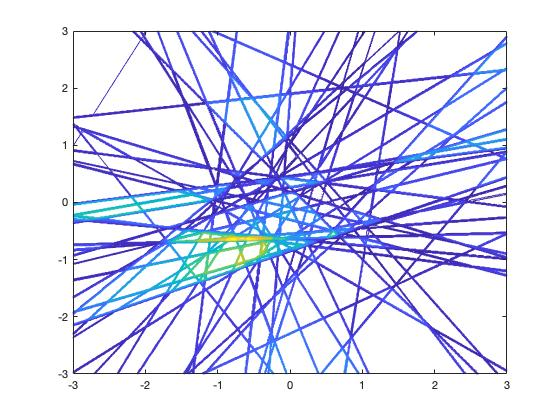
\includegraphics[width=.3\textwidth]{6dl/figures/dnn1-50.jpg}    
\end{center}
\caption{Hyperplanes with $\ell=1$, where $\ell$ is the depth of the neural network in \eqref{NNL}.}
\label{fig:1}
\end{figure} 		
 

The main goal of this section is to prove that the 
following type of error estimate holds, for some $\delta\ge 0$,
\begin{equation}\label{VNerror}
\inf_{v_N\in V_N^k}\|u- v_N \|_{H^m(\Omega)} \lesssim 
N^{-{1\over 2}-\delta}.
\end{equation} 
We will use two different approaches to establish \eqref{VNerror}.
The first approach, presented in \S\ref{sec:Bsplines}, mainly follows
\cite{hornik1994degree} and \cite{siegel2020approximations} that gives
error estimates for a general class of activation functions.  The
second approach follows
\cite{klusowski2016uniform} that gives error estimates specifically
for ReLU activation function.

We assume that $\Omega\subset\mathbb R^d$ is a given bounded domain.
Thus,
\begin{equation}
  \label{T}
T=\max_{x\in \bar{\Omega}} \|x\|<\infty.  
\end{equation}
The activation function ${\rm [ ReLU]}^k$ \eqref{relup} is related to
cardinal B-Splines.  A cardinal B-Spline of degree $k\ge 0$
denoted by $b^k$, is defined by convolution as
\begin{equation}
	b^k(x)=(b^{k-1}*b^0)(x)=\int_\mathbb{R}b^{k-1}(x-t)b^0(t)dt,
\end{equation}
where 
\begin{equation}
b^0(x)=\left\{
		     \begin{array}{lr}
		    1 & x\in[0,1),\\
		    0 & \hbox{otherwise}.
		     \end{array}
	\right.
\end{equation}
\begin{figure}
\begin{center}
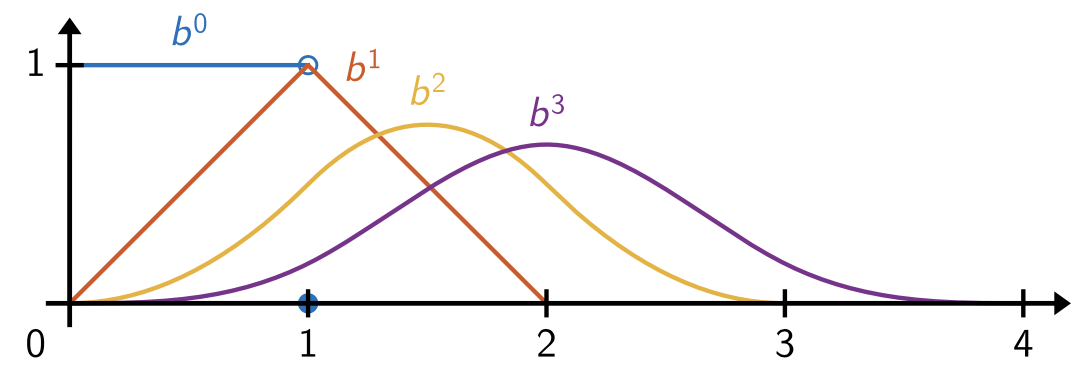
\includegraphics[width=0.5\textwidth]{6DL/figures/B-spline.png}   
\caption{Plots of some B-spline basis}
\label{bk}
\end{center}
\end{figure}
More explicitly, see \cite{de1971subroutine}, for any
$x\in[0,k+1]$ and $k\geq 1$, we have 
	\begin{equation}
	b^k(x)=\frac{x}{k}b^{k-1}(x)+\frac{k+1-x}{k}b^{k-1}(x-1),
	\end{equation}
or
	\begin{equation}\label{splinetorelu}
	b^k(x)=(k+1)\sum_{i=0}^{k+1} w_i(i-x)_+^k \hbox{~and~} w_i={\displaystyle\prod_{j=0,j\neq i}^{k+1}} \frac{1}{i-j}.
	\end{equation}
We note that all $b^k$ are locally supported and see Fig.~\ref{bk} for their plots. 

For an uniform grid with mesh size $h=\frac{1}{n+1}$, we define
	\begin{equation}
	b^k_{j,h}(x)=b^{k}(\frac{x}{h}-j).
	\end{equation}
Then the cardinal B-Spline series of degree $k$ on the uniform grid is 
\begin{equation}\label{Skn}
S_N^k=\Big\{v(x)=\sum_{j=-k}^{N}	c_jb^k_{j,h}(x)\Big\}.
\end{equation}
\begin{lemma} For $V_N^k$ and $S_N^k$ defined by \eqref{VkN} and
  \eqref{Skn}, we have
\begin{equation}
    \label{SV}
S_N^k\subset V_{N+k+1}^k.    
  \end{equation}
As a result, for any bounded domain $\Omega\subset \mathbb R^1$, we have
\begin{equation}
  \label{SVerror}
\inf_{v\in V_{N}^k}\|u-v\|_{m,\Omega} 
\le \inf_{v\in S_{N-k-1}^k}\|u-v\|_{m,\Omega} \lesssim N^{m-(k+1)} \|u\|_{k+1,\Omega}.
\end{equation}
\end{lemma}

\iffalse
Given an activation function $\sigma\in L^1(\mathbb R)$, consider its Fourier transformation:
\begin{equation}
  \label{Fsigma}
\hat \sigma(a) = \frac{1}{2\pi}\int_{\mathbb{R}} \sigma(t)e^{-iat}dt. 
\end{equation}
For any $a\neq 0$ with $\hat \sigma(a)\neq 0$, by making a change of variables 
$t = a^{-1}\omega\cdot x + b$ and $dt = db$, we have
 \begin{equation}
 \begin{aligned}
\hat{\sigma}(a)&=\frac{1}{2\pi}\int_{\mathbb{R}}\sigma(a^{-1}\omega\cdot x+b)e^{-ia( a^{-1}\omega\cdot x+b)}db = e^{-i\omega \cdot x}\frac{1}{2\pi}\int_{\mathbb{R}}\sigma(a^{-1} \omega\cdot x+b)e^{-iab}db.
 \end{aligned}
 \end{equation}
This implies that
\begin{equation}\label{FourierExp}
 e^{i\omega \cdot x} = \frac{1}{2\pi\hat{\sigma}(a)}\int_{\mathbb{R}}\sigma(a^{-1}\omega\cdot x+b)e^{-iab}db.
\end{equation}
We write $ \hat{u}(\omega) = e^{-i\theta(\omega)} | \hat{u}(\omega)|$
and then obtain the following integral represntation:
\begin{equation}\label{integral_representation01}
u(x) = \int_{\mathbb{R}^d} e^{i\omega\cdot x}\hat{u}(\omega)d\omega = 
\int_{\mathbb{R}^d}\int_\mathbb{R}\frac{1}{2\pi\hat{\sigma}(a)}
\sigma\left(a^{-1} \omega\cdot x+b\right)|\hat{u}(\omega)|e^{-i(ab+\theta(\omega))}dbd\omega
\end{equation}
Now we consider activation function $\sigma(x)=b^k(x)$ and $\hat \sigma$ be the
Fourier transform of $\sigma(x)$. Note that, by \eqref{bk}, 
\begin{align}\label{splineFourier}
\hat{\sigma}(a)=\left({1-e^{-ia}\over ia}\right)^{k+1}=\left({2\over a}\sin {a\over 2}\right)^{k+1}e^{-{ia(k+1)\over 2}}.
\end{align}

We first take $a=\pi$ in \eqref{splineFourier}. Thus,
\begin{equation}
  \label{pi1}
\hat\sigma(\pi)=
\left({2\over \pi}\right)^{k+1}e^{-{i\pi (k+1)\over 2}}.
\end{equation}
Combining \eqref{integral_representation01} and \eqref{pi1}, we obtain
that
\begin{equation}
  \label{splinerep0}
u(x) = 
\frac{1}{4}\left({\pi\over 2}\right)^{k}\int_{\mathbb{R}^d}\int_\mathbb{R}
\sigma\left(\pi^{-1}\omega\cdot x+b\right)|\hat{u}(\omega)|e^{-i(\pi b + {\pi (k+1)\over 2}+\theta(\omega))}dbd\omega
\end{equation}
An application of the Monte Carlo method in Lemma \ref{MC} to the integral representation \eqref{splinerep0} leads to the following estimate.
\begin{theorem}\label{splinestratify}
For any $0\le m\le k$, if $u\in {B}^{m+1}(\Omega)$, there exist $\omega_i\in \mathbb{R}^d$, $b_i\in \mathbb{R}$ such that
\begin{equation}
\left \|u - u_{N}\right\|_{H^{m}(\Omega)}\lesssim  N^{-{1\over 2}} \|u\|_{{B}^{m+1}(\Omega)}
\end{equation}
with
\begin{equation}
u_{N}(x)=\sum_{i=1}^{N} \beta_i b^k\left(\pi^{-1} \omega_i\cdot x+b_i\right).
\end{equation} 
\end{theorem}

Based on the integral representation \eqref{splinerep0}, a stratified analysis similar to the one in \cite{siegel2020approximations} leads to the following result.
\begin{theorem}
For any $0\le m\le k$ and positive $\epsilon$,  if $u\in {B}^{m+1+\epsilon}(\Omega)$, , there exist $\omega_i\in \mathbb{R}^d$, $b_i\in \mathbb{R}$ such that
\begin{equation}\label{straunbdd}
\left\|u - u_{N}\right\|_{H^{m}(\Omega)}\le  N^{-{1\over 2}-{\epsilon \over (d+1)(2+\epsilon)}} \|u\|_{{B}^{m+1+\epsilon}(\Omega)}
\end{equation}
with
\begin{equation}
u_{N}(x)=\sum_{i=1}^{N} \beta_i b^k\left(\bar \omega_i\cdot x+b_i\right) .
\end{equation} 
\end{theorem}
Next, we try to improve the estimate \eqref{straunbdd}. Again, we will use \eqref{integral_representation01}. Let $\displaystyle a_\omega=4\pi\lceil {\|\omega\|\over 4\pi}\rceil + \pi$ in \eqref{splineFourier} and $\displaystyle \bar\omega ={\omega\over a_\omega}$. We have
 \begin{equation}
\hat{\sigma}(a_\omega)=\left({2\over a_\omega}\right)^{k+1}, \quad \|\omega\| + \pi\le a_\omega\le \|\omega\|+5\pi,\quad \|\bar\omega\|\le 1,
 \end{equation}
which, together with \eqref{integral_representation01}, indicates that
 \begin{equation}\label{integral_representation}
 \begin{split}
  u(x) =  \int_{\mathbb{R}^d}\int_\mathbb{R}\frac{1}{2\pi}
  \sigma\left(\bar \omega\cdot x+b\right)\left({a_\omega\over 2}\right)^{k+1}\hat{u}(\omega)e^{-ia_\omega(b+{k+1\over 2})}dbd\omega.
\end{split}
 \end{equation}


\begin{theorem}
If $u\in {B}^{k+1}(\Omega)$, there exist $\|\bar \omega_i\|\le 1$, $|b_i|\le T + k+1$ such that
\begin{equation}\label{d+1}
\left\|u - u_{N}\right\|_{H^{m}(\Omega)}\lesssim  N^{-{1\over 2}-{1\over d+1}} \|u\|_{{B}^{k+1}(\Omega)}
\end{equation}
with
\begin{equation}
u_{N}(x)=\sum_{i=1}^{N} \beta_i b^k\left(\bar \omega_i\cdot x+b_i\right) .
\end{equation} 
\end{theorem}
\begin{proof}
We write \eqref{integral_representation} as follows
$$
\displaystyle u(x)= \int_{\mathbb{R}^d}\int_\mathbb{R}
g(x, b, \omega)\rho(b,\omega) dbd\omega
$$
with 
$$ 
\hat{u}(\omega) = e^{-i\theta(\omega)} | \hat{u}(\omega)|,\quad \tilde \theta(\omega)=\theta(\omega) + a_\omega(b+{k+1\over 2})
$$ and 
\begin{equation}\label{eq:g}
g(x, b, \omega) = \sigma\left({\bar \omega}\cdot x+b\right)sgn(\cos \tilde\theta(\omega)),
\end{equation}
\begin{equation}\label{eq:rho}
\rho(b,\omega) = \frac{1}{(2\pi)^d}\left({a_\omega\over 2}\right)^{k+1}| \hat{u}(\omega)||\cos \tilde\theta(\omega)|.
\end{equation} 
Note that
\begin{equation}
\|\bar\omega\|\le 1, \quad |b|\le T+k+1.
\end{equation} 
Let 
$$
G=\{(\omega, b): \omega\in \mathbb{R}^d,\ |b|\le T+k+1\}, \ \tilde G=\{(\bar \omega, b): \|\bar \omega\| \le 1,\ |b|\le T+k+1\}.
$$
For any positive integer $n$, divide $\tilde  G$ into $\tilde  M(\tilde  M\le {n\over 2})$   nonoverlapping subdomains, say 
$\tilde  G=\tilde  G_1\cup \tilde  G_2\cup \cdots \cup\tilde  G_{\tilde M}$, such that
\begin{equation}
|b-b'|\lesssim n^{-{1\over d+1}},\quad |\bar\omega - \bar\omega'|\lesssim  n^{-{1\over d+1}}, \quad (\bar\omega, b),\ (\bar\omega', b')\in \tilde G_i,\ 1\le i\le \tilde M.
\end{equation} 
Define $M=2\tilde  M$ and for $1\le i\le \tilde M$,
$$
G_i = \{(\omega, b): (\bar \omega, b)\in \tilde  G_i, \ \cos \tilde\theta(\omega)\ge 0\},\ 
G_{\tilde  M+i} = \{(\omega, b): (\bar \omega, b)\in \tilde  G_i, \ \cos \tilde\theta(\omega)\le 0\}.
$$
Thus, $G=G_1\cup G_2\cup \cdots \cup G_M$ with $\tilde  G_i\cap \tilde G_j=\varnothing$ if $i\neq j$, and 
\begin{equation}
|b-b'|\lesssim n^{-{1\over d+1}},\quad |\bar\omega - \bar\omega'|\lesssim  n^{-{1\over d+1}}, \quad sgn(\cos \tilde\theta(\omega))=sgn(\cos\tilde \theta(\omega')).
\end{equation} 
Let $n_i=\lceil \lambda(G_i)n\rceil$, $N=\displaystyle \sum_{i=1}^M n_i$ and
\begin{equation}
u_{N}(x)=\|\rho\|_{L^1(G)}\sum_{i=1}^{M} \frac{\lambda(G_{i})}{n_{i}} \sum_{j=1}^{n_{i}}g(x,\theta_{i,j}).
\end{equation}
It holds that
\begin{equation}\label{eq:sum}
\begin{split}
\mathbb{E}\left(\left\|u - u_{N}\right\|_{H^{m}(\Omega)}^{2}\right)\le&
\|\rho\|_{L^1(G)}\sum_{i=1}^{M}  \frac{\lambda^2(G_i)}{n_{i}}  \sup_{\theta_{i},\theta_{i}'\in G_i} \| g(x,\theta_i) - g(x,\theta_i')\|^2_{H^m(\Omega)}
 \end{split}
\end{equation}
with $\theta=(b, \omega)$. 
For any $(b, \omega)\in G_i$, $1\le i\le M$, if $k\ge m+1$,
\begin{equation}
|g(x,\theta) - g(x,\theta')| \lesssim |b-b'| + |\omega - \omega'| \lesssim   n^{-{1\over d+1}}
\end{equation}
Thus,
\begin{equation}
 \sum_{i=1}^{M}  \frac{\lambda^2(G_i)}{n_{i}}  \sup_{\theta_{i},\theta_{i}'\in G_i} \| g(x,\theta_i) - g(x,\theta_i')\|^2_{H^m(\Omega)}  
 \lesssim  n^{-{2\over d+1}} |\Omega|.
\end{equation}
Thus,
\begin{equation}\label{eq:}
\begin{split}
\mathbb{E}\left(\left\|u - u_{N}\right\|_{H^{m}(\Omega)}^{2}\right)\lesssim&   n^{-1-{2\over d+1}} |\Omega|\|\rho\|_{L^1(G)}.
 \end{split}
\end{equation}
Since $a\le \|\omega\|+5\pi$, 
$$
\|\rho\|_{L^1(G)}\lesssim \int_G (\|\omega\| + 1)^{k+1}|\hat u(\omega)|d\omega db \lesssim \|u\|_{B^{k+1}(\Omega)}.
$$
Note that $n\le N\le 2n$. Thus, there exist $\omega_i\in \mathbb{R}^d$, $\beta_i$, $b_i\in \mathbb{R}$ such that
\begin{equation}
\left\|u - u_{N}\right\|_{H^{m}(\Omega)}\lesssim  N^{-{1\over 2}-{1\over d+1}} \|u\|_{B^{k+1}(\Omega)},
\end{equation}
which completes the proof.
\end{proof}

The above analysis can also be applied to more general activation functions with compact support. 
\begin{theorem}
Suppose that $\sigma\in W^{m+1,\infty}(\mathbb{R})$ that has a compact
support. If for any $a>0$, there exists $\tilde a>0$ such that
\begin{equation}
\tilde a\gtrsim a,\quad  |\hat\sigma(\tilde a)|\gtrsim a^{-\ell},
\end{equation}
and  $u\in {B}^{\ell}(\Omega)$, then, there exist $\omega_i\in \mathbb{R}^d$ and $b_i\in \mathbb{R}$ such that
\begin{equation}
\left\|u - u_{N}\right\|_{H^{m}(\Omega)}\lesssim  N^{-{1\over 2}-{1\over d+1}} \|u\|_{B^{\ell}(\Omega)},
\end{equation}
where
\begin{equation}
u_{N}(x)=\sum_{i=1}^{N} \beta_i \sigma\left(\bar \omega_i\cdot x+b_i\right) .
\end{equation} 
\end{theorem}

\fi

%\subsection{ReLU Fourier representation }%-- Simple version}

We introduce the Taylor expansion of $e^{iz}$ with integral remainder as follows.
\begin{lemma}
For $|z|\leq c$, 
\begin{equation}  
e^{iz} -  iz -1
= 
- \int_{0}^c\left[(z - u)_+e^{iu} + (-z - u)_+e^{-iu} \right]du.
\end{equation}  
\end{lemma}
\begin{proof}  
By the Taylor expansion with integral remainder,
\begin{equation} 
e^{iz} = 1 + iz  - \int_0^z e^{iu}(z-u)du.
\end{equation}
Let $u_+=\max (u, 0)$ and $u_-=\min(u,0)$. Then, $u_-=-(-u)_+$ and 
$$
z-u=(z-u)_+ + (z-u)_-=(z-u)_+ - (u-z)_+.
$$
It follows that
\begin{equation}
\begin{split}
\int_{0}^z (z-u)e^{iu} du=&\int_{0}^z (z-u)_+e^{iu} du + \int_{0}^z -(u-z)_+e^{iu} du
\\
=&\int_{0}^z (z-u)_+e^{iu} du + \int_{0}^{-z}  (-u-z)_+e^{-iu} du
\\
=&\int_{0}^c (z-u)_+e^{iu} du + (-u-z)_+e^{-iu} du.
\end{split}
\end{equation}
Thus,
\begin{equation}  
e^{iz} - 1 - iz 
= 
-\int_{0}^c\left[(z - u)_+e^{iu} + (-z - u)_+e^{-iu} \right]du,
\end{equation}  
which completes the proof.
\end{proof}

Let $z=\omega\cdot x$, $u=\|\omega\|_{\ell_1}t$ and $\bar \omega={\omega\over \|\omega\|_{\ell_1}}$. If $\Omega$ is bounded, say $|x|\le T$, $|\bar \omega \cdot x|\le T$. There exists the following expansion for $e^{i\omega\cdot x}$.
\begin{lemma}\label{lm:talorcomplex}
If $|x|\le T$,
\begin{equation}  
e^{i\omega\cdot x} - 1 -  i\omega\cdot x 
= 
- \|\omega\|_{\ell_1}^2\int_{0}^T\left[(\bar \omega\cdot x - t)_+e^{i\|\omega\|_{\ell_1}t}
+ (-\bar \omega\cdot x - t)_+e^{-i\|\omega\|_{\ell_1}t} \right]dt.
\end{equation} 
Denote 
$$
D^\alpha = \partial_1^{\alpha_1}\partial_2^{\alpha_2}\cdots \partial_d^{\alpha_d},\quad \omega^\alpha = \omega_1^{\alpha_1}\omega_2^{\alpha_2}\cdots \omega_d^{\alpha_d},\quad \alpha!=\alpha_1!\alpha_2!\cdots \alpha_d!.
$$
\end{lemma}
It follows  the following Taylor expansion with an integral remainder.
\begin{lemma}\label{lm:probabilityexpan}
Suppose $|x|\le T$. There exists
\begin{equation}
f(x) = f(0) + \nabla f(0)\cdot x
+  \int_{\{-1,1\}\times [0,T]\times \mathbb{R}^{d}}  g(x, \theta)\lambda(\theta)d\theta  
\end{equation}  
with  $g(x,\theta)$ and $\lambda(\theta)$ defined in \eqref{eq:straglam}.
\end{lemma}
\begin{proof}
Since $
 f(x) = \int_{\mathbb{R}^d} e^{i\omega\cdot x}\hat{f}(\omega)d\omega
$
and 
$
\nabla f(x)=\int_{\mathbb{R}^d} i^{|\alpha|}\omega  e^{i\omega\cdot x}\hat{f}(\omega)d\omega,
$
\begin{eqnarray}
\nabla  f(0)\cdot x=\int_{\mathbb{R}^d} i\omega\cdot  x\hat{f}(\omega)d\omega.
\end{eqnarray} 
 It follows that
\begin{equation}
\nabla  f(0) \cdot x=i \int_{\mathbb{R}^d} \omega\cdot x\hat{f}(\omega)d\omega
=  \int_{\mathbb{R}^d} i\omega\cdot x\hat{f}(\omega)d\omega.
\end{equation} 
Let $\hat{f}(\omega)=|\hat{f}(\omega)|e^{ib(\omega)}$. Then, $e^{i\|\omega\|_{\ell_1}t}\hat{f}(\omega) = |\hat{f}(\omega)|e^{i(\|\omega\|_{\ell_1}t + b(\omega))}$.
By Lemma \ref{lm:talorcomplex},
\begin{equation}\label{eq:fftaylor}
\begin{split}
&f(x) - f(0) - \nabla  f(0) \cdot x
\\
= &\int_{\mathbb{R}^d} \big (e^{i\omega\cdot x} - 1 - i\omega\cdot x \big )\hat{f}(\omega)d\omega.
\\
=&{\rm Re} \bigg (-\int_{\mathbb{R}^d} \int_{0}^T\left[(\bar \omega\cdot x - t)_+e^{i\|\omega\|_{\ell_1}t}
+ (-\bar \omega\cdot x - t)_+e^{-i\|\omega\|_{\ell_1}t} \right]\hat{f}(\omega)\|\omega\|_{\ell_1}^{2}dt d\omega\bigg )
\\
=& \int_{\{-1,1\}}\int_{\mathbb{R}^d} \int_{0}^T (z\bar \omega\cdot x - t)_+ s(zt,\omega)  |\hat{f}(\omega)|\|\omega\|_{\ell_1}^{2}dtd\omega dz
\end{split}
\end{equation}
with $\int_{\{-1, 1\}} r(z) dz = r(-1) + r(1)$ and
\begin{equation} 
s(zt,\omega)= -\cos(z\|\omega\|_{\ell_1}t + b(\omega)) 
\end{equation} 
Define $G=\{-1,1\}\times [0,T]\times \mathbb{R}^{d}$, $\theta=(z, t, \omega)\in G$,
\begin{equation}\label{eq:straglam}
g(x,\theta)= (z\bar \omega\cdot x - t)_+ {\rm sgn} s(zt,\omega),\qquad \lambda(\theta)={\rho(\theta)\over 
\int_{\{-1,1\}\times [0,T]\times \mathbb{R}^{d}} \rho(\theta)d\theta}.
\end{equation}
with $\rho(\theta) = |s(zt,\omega)||\hat{f}(\omega)|\|\omega\|_{\ell_1}^{2}$. 

Then \eqref{eq:fftaylor} can be written as 
\begin{equation}\label{eq:reluintegral}
f(x) = f(0) +  \nabla  f(0) \cdot x
+  \int_{\{-1,1\}\times [0,T]\times \mathbb{R}^{d}}  g(x, \theta)\lambda(\theta)d\theta,  
\end{equation}   
which completes the proof.
\end{proof}

An application of the Monte Carlo method in Lemma \ref{MC} to the integral \eqref{eq:reluintegral} gives the following estimate.
\begin{theorem} 
Suppose $|x|\le T$ and 
$$
 \int_{\mathbb{R}^{d}} |\hat{f}(\omega)|\|\omega\|_{\ell_1}^{2} d\omega<\infty.
$$
There exist  $\|\bar \omega_j\|_{\ell_1}=1$, $t\in [0,T]$ such that 
$$
f_n(x)= f(0) + \nabla  f(0) \cdot x  + {1\over n}\sum_{j=1}^{n} (\bar \omega_j\cdot x - t_j)_+
$$ 
satisfies the following estimate 
\begin{equation}
\|f - f_n \|_{L^2(\Omega)} \leq C n^{-{1\over 2}}.
\end{equation} 
%\begin{equation}
%\|D^\beta (f(x)- f_n(x))\|_{L^2(\Omega)}\le \sqrt{2^{m-k-2}(2m-k)\over k!(m-k)!}|\Omega|^{1/2} n^{-{1\over 2}-{1\over d}},\quad |\beta|=k\le m.
%\end{equation}
\end{theorem}

\iffalse
\noindent\textbf{A modified analysis using stratified sampling}

According to \eqref{eq:straglam}, the main ingredient $(z\bar \omega\cdot x - t)_+$ of $g(x,\theta)$  only includes the direction $\bar\omega$ of $\omega$ which belongs to a bounded domain  $\mathbb{S}^{d-1}$. Thanks to the continuity of $(z\bar \omega\cdot x - t)_+$ with respect to $(z, \bar\omega, t)$ and the boundedness of $\mathbb{S}^{d-1}$,
the application of the stratified sampling to the residual term of the Taylor expansion leads to the following approximation property.
\begin{theorem}\label{est:stratify}
Suppose $|x|\le T$ and 
$$
 \int_{\mathbb{R}^{d}} |\hat{f}(\omega)|\|\omega\|_{\ell_1}^{2} d\omega<\infty.
$$
There exist $\beta_j\in [-2^d,2^d]$, $\|\bar \omega_j\|_{\ell_1}=1$, $t\in [0,T]$ such that 
$$
f_n(x)= f(0) + \nabla  f(0) \cdot x  + {1\over n}\sum_{j=1}^{n}\beta_j (\bar \omega_j\cdot x - t_j)_+
$$ 
satisfies the following estimate 
\begin{equation}
\|f - f_n \|_{L^2(\Omega)} \leq C n^{-{1\over 2}-{1\over d}}.
\end{equation} 
%\begin{equation}
%\|D^\beta (f(x)- f_n(x))\|_{L^2(\Omega)}\le \sqrt{2^{m-k-2}(2m-k)\over k!(m-k)!}|\Omega|^{1/2} n^{-{1\over 2}-{1\over d}},\quad |\beta|=k\le m.
%\end{equation}
\end{theorem}
\begin{proof}
By Lemma \ref{lem:stratifiedapprox}, for any decomposition $G=\cup_{i=1}^M G_i$, there exist $\{\theta_i\}_{i=1}^n$ and $\{\beta_i\}_{i=1}^n\in [0,1]$ such that 
\begin{equation}
\|  f - f_n\|_{L^2(\Omega)} = \|  r - r_{n}\|_{L^2(\Omega)} \leq {1\over n^{1/2}}\max_{1\le j\le M}\sup_{\theta_{j},\theta_{j}'\in G_j} \|   g(x,\theta_j) - g(x,\theta_j') \|_{L^2(\Omega)} 
\end{equation}
with 
$$
f_n(x)= f(0) +  \nabla  f(0) \cdot x + r_{n}(x), \qquad r_{n}(x)={1\over n}\sum_{j=1}^{n}\beta_j (\bar \omega_j\cdot x - t_j)_+, 
$$
$$
r(x)=\int_{\{-1,1\}\times [0,T]\times \mathbb{R}^{d}}  g(x, \theta)\lambda(\theta)d\theta.
$$
Consider a particular decomposition $G=\cup_{i=1}^M G_i$ as follows. 
The variable $z$ is in the set $\{-1,1\}$, which can be divided into two subsets $\{-1\}$ and $\{1\}$. 
Given a positive integer $n$, for the random variable $t$, the interval  $ [0,T]$ can be divided into $n_t$ subintervals $\{G_i^t\}_{i=1}^{n_t}$ such that 
$$
|t-t'|<{1\over 2}n^{-{1\over d}}\quad t,t'\in G_i^t,\quad 1\leq i\leq n_t
$$ 
for $n_t>2\lceil T  n^{1\over d}\rceil$. 
For variable $\bar \omega=\omega/\|\omega\|_{\ell_1}\in \mathbb{S}^{d-1}$ where $\mathbb{S}^{d-1}=\{\bar \omega\in \mathbb{R}^d: \|\bar \omega\|_{\ell_1}=1\}$. Note that $\mathbb{S}^{d-1}$ can be divided into $n_\alpha$ subdomains $\{G_i^s \}_{i=1}^{n_s}$ such that
$$
\|\bar \omega- \bar \omega'\|_{\ell_1}\leq {1\over 2}n^{-{1\over d}}\qquad \bar \omega, \bar \omega' \in G_i^s,\quad 1\leq i\leq n_s
$$
for $(2n^{1\over d})^{d-1}\leq n_s\leq \lceil (5n^{1\over d})^{d-1}\rceil$ \cite{klusowski2016uniform}.
Then 
$$
G=\displaystyle \cup \{G_{ijk\ell}: 1\leq i\leq 2,\ 1\leq j\leq n_t,\ 1\leq k\leq n_s,\ 1\le \ell\le 2\}
$$
with 
\begin{equation}
G_{ijk\ell} = \{(z, t, \omega): z=(-1)^i,\ t\in G_j^t, \bar \omega \in G_k^s,\ {\rm sgn} s(zt,\omega)=(-1)^\ell\}.
\end{equation}
Denote this decomposition of $G$ by $G=\cup_{i=1}^{M} G_i$ with $M=4n_sn_t\le 2^{d}n$. For each $G_i$,
\begin{equation}
z=z',\ |t-t'|<{1\over 2}n^{-{1\over d}},\ \|\bar \omega  - \bar \omega'\|_{\ell^1}<{1\over 2}n^{-{1\over d}}\qquad \forall \theta=(z, t, \omega),\ \theta'=(z', t', \omega')\in G_i.
\end{equation}
For any $\theta_i, \theta'_i\in G_i$ and $|\alpha |=1$,  
$$
| g(x,\theta_i) - g(x,\theta_i') | =  | \bar\omega  -   \bar\omega' |\le n^{-{1\over d}}.
$$  
Thus, there exist $\theta_{i,j}$ such that
\begin{equation}
\| f - f_n\|_{L^2(\Omega)} \le C  n^{-{1\over 2}-{1\over d}}.
\end{equation}
with
$$
f_n(x)=  f(0) + \nabla f(0) \cdot x + {1\over  n}\sum_{j=1}^{n}\beta_j (\bar \omega_j\cdot x - t_j)_+
$$ 
with $\beta_j\in [-2^d,2^d]$,
which completes the proof.
\end{proof}


\fi
 

















%\section{ReLU Fourier representation}\label{sec:error2}
Rather than using general Fourier transform  to represent
$e^{i\omega\cdot x}$ in terms of $\sigma(\omega\cdot x+b)$, 
\cite{klusowski2016uniform} gave a different method to represent
$e^{i\omega\cdot x}$ in terms of $(\omega\cdot x+b)_+^k$  for $k=1$
and $2$.   The following lemma gives a generalization of this
representation for all $k\ge 0$. 
\begin{lemma}\label{lm:talorcomplex}
For any $k\ge0$ and $x\in \Omega$,
\begin{equation}  
e^{i\omega\cdot x} =\sum_{j=0}^k{(i\omega\cdot x)^{j}\over j!} 
+
{i^{k+1}\over k!} \|\omega\|^{k+1}\int_{0}^T\left[(\bar \omega\cdot x - t)_+^ke^{i\|\omega\|t}
+(-1)^{k-1}(-\bar \omega\cdot x - t)_+^ke^{-i\|\omega\|t} \right]dt.
\end{equation} 
\end{lemma}
\begin{proof}  
For $|z|\leq c$, by the Taylor expansion with integral remainder,
\begin{equation} 
e^{iz} = \sum_{j=0}^k {(iz)^j\over j!} + {i^{k+1}\over k!} \int_0^z e^{iu}(z-u)^kdu.
\end{equation}
Note that 
$$
(z-u)^k=(z-u)^k_+ - (u-z)^k_+.
$$
It follows that
\begin{equation}
\begin{split}
\int_{0}^z (z-u)^ke^{iu} du=&\int_{0}^z (z-u)_+^ke^{iu} du + \int_{0}^z (-1)^k(u-z)_+^ke^{iu} du
\\
=&\int_{0}^z (z-u)_+^ke^{iu} du + \int_{0}^{-z} (-1)^{k-1}(-u-z)_+^ke^{-iu} du
\\
=&\int_{0}^c (z-u)_+^ke^{iu} du + (-1)^{k-1}(-u-z)_+^ke^{-iu} du.
\end{split}
\end{equation}
Thus,
\begin{equation}  
e^{iz} - \sum_{j=0}^k{(iz)^{j}\over j!} 
= 
{i^{k+1}\over k!}\int_{0}^c\left[(z - u)_+^ke^{iu} + (-1)^{k-1}(-z - u)_+^ke^{-iu} \right]du.
\end{equation}  
Let 
\begin{equation}\label{baromega}
z=\omega\cdot x,\quad u=\|\omega\|t,\quad \bar \omega={\omega\over \|\omega\|}.
\end{equation}
Since $\|x\| \le T$ and $|\bar \omega \cdot x|\le T$, we obtain
\begin{equation}  
e^{i\omega\cdot x} - \sum_{j=0}^k{(i\omega\cdot x)^{j}\over j!} 
= 
{i^{k+1}\over k!} \|\omega\|^{k+1}\int_{0}^T\left[(\bar \omega\cdot x - t)_+^ke^{i\|\omega\|t}
+(-1)^{k-1}(-\bar \omega\cdot x - t)_+^ke^{-i\|\omega\|t} \right]dt,
\end{equation} 
which completes the proof.
\end{proof}

Since $
u(x) = {1\over (2\pi)^d}\int_{\mathbb{R}^d} e^{i\omega\cdot x}\hat{u}(\omega)d\omega
$
and 
$
 \partial^\alpha u(x)=\int_{\mathbb{R}^d} i^{|\alpha|}\omega^\alpha e^{i\omega\cdot x}\hat{u}(\omega)d\omega,
$
\begin{eqnarray}
 \partial^\alpha u(0)x^\alpha=\int_{\mathbb{R}^d} i^{|\alpha|}\omega^\alpha x^\alpha\hat{u}(\omega)d\omega.
\end{eqnarray} 
Note that $\displaystyle (\omega\cdot x)^j=\sum_{|\alpha|=j}{j!\over \alpha !}\omega^\alpha x^\alpha $. It follows that
\begin{equation}
\sum_{|\alpha|=j}{1\over \alpha!} \partial^\alpha u(0) x^\alpha=i^j\sum_{|\alpha|=j}{1\over \alpha!} \int_{\mathbb{R}^d} \omega^\alpha x^\alpha\hat{u}(\omega)d\omega
={1\over j!}  \int_{\mathbb{R}^d} (i\omega\cdot x)^j \hat{u}(\omega)d\omega.
\end{equation} 
Let $\hat{u}(\omega)=|\hat{u}(\omega)|e^{ib(\omega)}$. Then, $e^{i\|\omega\|t}\hat{u}(\omega) = |\hat{u}(\omega)|e^{i(\|\omega\|t + b(\omega))}$.
By Lemma \ref{lm:talorcomplex},
\begin{equation}\label{eq:fftaylor}
\begin{split}
&u(x) - \sum_{|\alpha|\le k}{1\over \alpha!} \partial^\alpha u(0) x^\alpha
\\
= &\int_{\mathbb{R}^d} \big (e^{i\omega\cdot x}-\sum_{j=0}^k{1\over j!}(i\omega\cdot x)^j\big )\hat{u}(\omega)d\omega.
\\
=&{\rm Re} \bigg ({i^{k+1}\over k!}\int_{\mathbb{R}^d} \int_{0}^T\left[(\bar \omega\cdot x - t)_+^ke^{i\|\omega\|t}
+(-1)^{k-1}(-\bar \omega\cdot x - t)_+^ke^{-i\|\omega\|_{\ell_1}t} \right]\hat{u}(\omega)\|\omega\|^{k+1}dt d\omega\bigg )
\\
=& {1\over k!}\int_{\{-1,1\}}\int_{\mathbb{R}^d} \int_{0}^T (z\bar \omega\cdot x - t)_+^k s(zt,\omega)  |\hat{u}(\omega)|\|\omega\|^{k+1}dtd\omega dz
\end{split}
\end{equation}
with $\int_{\{-1, 1\}} r(z) dz = r(-1) + r(1)$ and
\begin{equation} 
s(zt,\omega)= 
\begin{cases}
(-1)^{k+1\over 2}\cos(z\|\omega\|t + b(\omega)) & k \text{ is odd},
\\
(-1)^{k+2\over 2}\sin(z\|\omega\|t + b(\omega)) & k \text{ is even}.
\end{cases}
\end{equation} 
Define $G=\{-1,1\}\times [0,T]\times \mathbb{R}^{d}$, $\theta=(z, t, \omega)\in G$,
\begin{equation}\label{eq:straglam}
g(x,\theta)= (z\bar \omega\cdot x - t)_+^k {\rm sgn} s(zt,\omega),\qquad  \rho(\theta) = {1\over (2\pi)^d}|s(zt,\omega)||\hat{u}(\omega)|\|\omega\|^{k+1},\quad \lambda(\theta)={\rho(\theta)\over 
\|\rho\|_{L^1(G)}}.
\end{equation} 

Then \eqref{eq:fftaylor} can be written as 
\begin{equation}
u(x) = \sum_{|\alpha|\le k}{1\over \alpha!}D^\alpha u(0) x^\alpha
+ {\nu\over k!}\int_G  g(x, \theta)\lambda(\theta)d\theta,  
\end{equation}   
with $\nu=\int_G \rho(\theta)d\theta$. In summary, we have the following lemma.
 


\begin{lemma}\label{lm:probabilityexpan}
It holds that
\begin{equation}\label{ReLUm}
u(x) = \sum_{|\alpha|\le k}{1\over \alpha!} \partial^\alpha u(0) x^\alpha
+ {\nu\over k!}r_k(x),\qquad x\in \Omega
\end{equation}  
with $\nu=\int_G \rho(\theta)d\theta$ and 
\begin{equation}\label{ReLUrm}
r_k(x) = \int_G  g(x, \theta)\lambda(\theta)d\theta,\qquad G=\{-1,1\}\times [0,T]\times \mathbb{R}^{d},
\end{equation}  
and  $g(x,\theta)$, $\rho(\theta)$  and $\lambda(\theta)$ defined in \eqref{eq:straglam}.
\end{lemma}

According to \eqref{eq:straglam}, the main ingredient $(z\bar
\omega\cdot x - t)_+^k$ of $g(x,\theta)$ only includes the direction
$\bar\omega$ of $\omega$ which belongs to a bounded domain
$\mathbb{S}^{d-1}$. Thanks to the continuity of $(z\bar \omega\cdot x
- t)_+^k$ with respect to $(z, \bar\omega, t)$ and the boundedness of
$\mathbb{S}^{d-1}$, the application of the stratified sampling to the
residual term of the Taylor expansion leads to the 
approximation property in Theorem \ref{est:stratify}.

\begin{theorem}\label{est:stratify}
Assume $u\in B^{k+1}(\Omega)$
%$$
% \int_{\mathbb{R}^{d}} |\hat{f}(\omega)|\|\omega\|^{m+1} d\omega<\infty.
%$$
There exist $\beta_j\in [-1, 1]$, $\|\bar \omega_j\|=1$, $t_j\in [0,T]$ such that 
\begin{equation}
u_N(x)= \sum_{|\alpha|\le k}{1\over \alpha!} \partial^\alpha u(0) x^\alpha + {2\nu\over k!N}\sum_{j=1}^{N}\beta_j (\bar \omega_j\cdot x - t_j)_+^k
\end{equation} 
with $\nu=\int_G \rho(\theta)d\theta$ and $\rho(\theta)$  defined in \eqref{eq:straglam} 
satisfies the following estimate
\begin{equation}
\|u - u_N \|_{H^m(\Omega)} \lesssim  
\begin{cases}
 N^{-{1\over 2}-{1\over d}}\|u\|_{B^{k+1}(\Omega)},&m< k,
\\
N^{-{1\over 2}}\|u\|_{B^{k+1}(\Omega)}& m=k.
\end{cases} 
\end{equation} 
%Especially,
%\begin{equation}
%\|u - u_N \|_{L^2(\Omega)} \leq {(2T)^k|\Omega|^{1\over 2}\over (k-1)!} N^{-{1\over 2}-{1\over d}}\|u\|_{\mathcal B^{k+1, q}(\Omega)}.
%\end{equation} 
%\begin{equation}
%\|D^\beta (f(x)- f_n(x))\|_{L^2(\Omega)}\le \sqrt{2^{m-k-2}(2m-k)\over k!(m-k)!}|\Omega|^{1/2} n^{-{1\over 2}-{1\over d}},\quad |\beta|=k\le m.
%\end{equation}
\end{theorem}

\begin{proof}
Let
$$
u_N(x)=  \sum_{|\alpha|\le k}{1\over \alpha!} \partial^\alpha u(0) x^\alpha + {\nu\over k!} r_{k,N}(x), \qquad r_{k,N}(x)={1\over N}\sum_{j=1}^{N}\beta_j (\bar \omega_j\cdot x - t_j)_+^k.
$$
Recall  the representation  of $u(x)$ in \eqref{ReLUm} and $r_k(x)$ in \eqref{ReLUrm}. It holds that
\begin{equation}
u(x) - u_N(x)={2\nu\over k!} (r_k(x) - r_{k,N}(x)).
\end{equation}
By Lemma \ref{lem:stratifiedapprox}, for any decomposition $\displaystyle G=\cup_{i=1}^N G_i$, there exist $\{\theta_i\}_{i=1}^N$ and $\{\beta_i\}_{i=1}^N\in [0, 1]$ such that 
\begin{equation}
\| \partial_x^\alpha (u - u_N)\|_{L^2(\Omega)} = {\nu\over k!}\|  \partial_x^\alpha (r_k - r_{k,N})\|_{L^2(\Omega)} \leq {1\over k!N^{1/2}}\max_{1\le j\le n}\sup_{\theta_{j},\theta_{j}'\in G_j} \|  \partial_x^\alpha \big(g(x,\theta_j) - g(x,\theta_j')\big)\|_{L^2(\Omega)}.
\end{equation}
\iffalse
Consider a $\epsilon$-covering decomposition $G=\cup_{i=1}^M G_i$ as follows. 
The variable $z$ is in the set $\{-1,1\}$, which can be divided into two subsets $\{-1\}$ and $\{1\}$. 
Given a positive integer $N$, for the random variable $t$, the interval  $ [0,T]$ can be divided into $n_t$ subintervals $\{G_i^t\}_{i=1}^{n_t}$ such that 
$$
|t-t'|<{1\over 2}N^{-{1\over d}}\quad t,t'\in G_i^t,\quad 1\leq i\leq n_t
$$ 
for $n_t>2\lceil T N^{1\over d}\rceil$. 
For variable $\bar \omega=\omega/\|\omega\|\in \mathbb{S}^{d-1}$ where $\mathbb{S}^{d-1}=\{\bar \omega\in \mathbb{R}^d: \|\bar \omega\|=1\}$. Note that $\mathbb{S}^{d-1}$ can be divided into $n_\alpha$ subdomains $\{G_i^s \}_{i=1}^{n_s}$ such that
$$
\|\bar \omega- \bar \omega'\|\leq {1\over 2}N^{-{1\over d}}\qquad \bar \omega, \bar \omega' \in G_i^s,\quad 1\leq i\leq n_s
$$
for $(2N^{1\over d})^{d-1}\leq n_s\leq \lceil (5N^{1\over d})^{d-1}\rceil$ \cite{klusowski2016uniform}.
Then 
$$
G=\displaystyle \cup \{G_{ijk\ell}: 1\leq i\leq 2,\ 1\leq j\leq n_t,\ 1\leq k\leq n_s,\ 1\le \ell\le 2\}
$$
with 
\begin{equation}
G_{ijk\ell} = \{(z, t, \omega): z=(-1)^i,\ t\in G_j^t, \bar \omega \in G_k^s,\ {\rm sgn} s(zt,\omega)=(-1)^\ell\}.
\end{equation}
Denote this decomposition of $G$ by $G=\cup_{i=1}^{M} G_i$ with $M=4n_sn_t\le 2^{d}N$. For each $G_i$,
\fi
Consider a $\epsilon$-covering decomposition $G=\cup_{i=1}^N G_i$  such that 
\begin{equation}
z=z',\ |t-t'|<\epsilon,\ \|\bar \omega  - \bar \omega'\|_{\ell^1}<\epsilon\qquad \forall \theta=(z, t, \omega),\ \theta'=(z', t', \omega')\in G_i
\end{equation}
where $\bar\omega$ is defined in \eqref{baromega}. 
For any $\theta_i, \theta'_i\in G_i$,  
$$
| \partial_x^\alpha \big (g(x,\theta_i) - g(x,\theta_i')\big )| = {k!\over (k-|\alpha|)!} | g_\alpha(x, \bar\omega, t) -  g_\alpha(x, \bar\omega', t')| 
$$
with 
\begin{equation}
 g_\alpha(x, \bar\omega, t)  = (z\bar \omega\cdot x-t)^{k-|\alpha|}_+\bar \omega^\alpha.
 \end{equation} 
 Since
$$
|\partial_{\bar\omega_i}  g_\alpha|\le (2T)^{m-|\alpha|-1}\big ((k-|\alpha|)x_i + 2T\alpha_i\big ), \qquad |\partial_t  g_\alpha|\le (k-|\alpha|)(2T)^{k-|\alpha|-1},
$$
it follows that
\begin{equation}
\big | \partial_x^\alpha \big (g(x,\theta_i) - g(x,\theta_i')\big )\big | \le {k!\over (k-|\alpha|)!}(2T)^{k-|\alpha|-1}   \bigg ( (k-|\alpha|)(|x|_{\ell_1}+1) + 2T|\alpha |\bigg ) \epsilon.
\end{equation}
Thus, by Lemma \ref{lem:stratifiedapprox}, if $m=|\alpha|<k$,
\begin{equation}
\|  \partial_x^\alpha (u - u_N)\|_{L^2(\Omega)} \le {|\Omega|^{1/2}\over (k-|\alpha|)!}(2T)^{k-|\alpha|-1}   \bigg ( (k-|\alpha|)(T+1) + 2T|\alpha |\bigg )N^{-{1\over 2}}\epsilon.
\end{equation}
Note that $\epsilon \sim N^{-{1\over d}}$. There exist $\theta_{i,j}$ such that for any $0\le k< m$,
\begin{equation}
\| u - u_N\|_{H^k(\Omega)} \le  C(m,k,\Omega)\nu N^{-{1\over 2}-{1\over d}}
\end{equation}
with $\nu\le \|u\|_{B^{k+1}(\Omega)}$ and
\begin{equation}\label{equ:defcmko}
C(m,k,\Omega)=|\Omega|^{1/2}\bigg (\sum_{|\alpha|\le k}{1\over (k-|\alpha|)!}(2T)^{k-|\alpha|-1}   \big ( (k-|\alpha|)(T+1) + 2T|\alpha |\big )\bigg )^{1/2}.
\end{equation} 
If $m=|\alpha|=k$,
$$
\max_{1\le j\le M}\sup_{\theta_{j},\theta_{j}'\in G_j} \| D_x^\alpha \big(g(x,\theta_j) - g(x,\theta_j')\big)\|_{L^2(\Omega)}\lesssim 1.
$$
This leads to 
\begin{equation}
\| u - u_N\|_{H^m(\Omega)} \le  C(m,k,\Omega)\nu N^{-{1\over 2}}\quad \mbox{for }\ k=m.
\end{equation}
Note that $u_N$ defined above can be written as
$$
u_N(x)=  \sum_{|\alpha|\le k}{1\over \alpha!} \partial^\alpha u(0) x^\alpha + {1\over k!N}\sum_{j=1}^{N}\beta_j (\bar \omega_j\cdot x - t_j)_+^k
$$ 
with $\beta_j\in [-1, 1]$,
which completes the proof.
\end{proof}

\begin{lemma}
There exist $\alpha_i$, $\omega_i$, $b_i$ and $N\le 2\begin{pmatrix} k+d\\k\end{pmatrix}$
such that
$$
 \sum_{|\alpha|\le m}{1\over \alpha!} \partial^\alpha u(0) x^\alpha = \sum_{i=1}^N\alpha_i (\omega_i\cdot x + b_i)_+^k
$$ 
with $
x^\alpha = x_1^{\alpha_1}x_2^{\alpha_2}\cdots x_d^{\alpha_d},\quad \alpha!=\alpha_1!\alpha_2!\cdots \alpha_d!.
$
\end{lemma}
The above result can be found in \cite{he2020preprint}

A combination of Theorem \ref{est:stratify} and the above the lemma gives the following estimate in Theorem \ref{th:stra}.
\begin{theorem} \label{th:stra}
Suppose $u\in B^{k+1}(\Omega)$.
There exist $\beta_j, t\in \mathbb{R}$, $\omega_j \in \mathbb{R}^d$ such that 
\begin{equation}
u_N(x)= \sum_{j=1}^{N}\beta_j (\bar \omega_j\cdot x - t_j)_+^k
\end{equation} 
satisfies the following estimate
\begin{equation}\label{d}
\|u- u_N \|_{H^m(\Omega)} \lesssim 
\begin{cases}
N^{-{1\over 2}-{1\over d}}\|u\|_{B^{k+1}(\Omega)},\qquad k> m,
\\
N^{-{1\over 2}}\|u\|_{B^{k+1}(\Omega)},\qquad k= m,
\end{cases}
\end{equation} 
where $\bar\omega$ is defined in \eqref{baromega}.
\end{theorem}

\begin{remark}
We make the following comparisons:
\begin{enumerate}
\item The results in \ref{sec:Bsplines} are for activation functions $\sigma=b_k$, while the results in Section \ref{sec:error2} are for activation functions $\sigma={\rm ReLU}^k$.
\item By \eqref{splinetorelu}, the following relation obviously holds
$$
V_N(b_k)\subset V_{N+k}({\rm ReLU}^k),
$$
where 
\begin{equation}
\label{VkN}
V_{N+k}({\rm ReLU}^k)=\left\{\sum_{i=1}^Na_i(w_i\cdot x+b_i)_+^k, a_i, b_i\in\mathbb R^1, w_i\in \mathbb R^{1\times d}\right\},
\end{equation}
and $V_N(b_k)$ is the one hidden layer neuron network
function class with activation function $b_k$.  Thus, asymptotically
speaking, the results that hold for $\sigma=b_k$ also hold for
$\sigma={\rm ReLU}^k$. 
\end{enumerate}
\end{remark}







\subsection{Periodic activation function}
By dilating $\sigma$ if necessary, we may assume without loss of generality that $\sigma$ is periodic on $[0,1]$. Consider the Fourier series of $\sigma$
\begin{equation}
\sigma(x) = \displaystyle\sum_{i=-\infty}^\infty a_i e^{2\pi ix},
\end{equation}
with coefficients
\begin{equation}\label{eq_1027}
a_i =  \int_0^{1} \sigma(b)e^{-2\pi ib}db. 
\end{equation}
The assumption that $\sigma$ is non-constant means that there exists some $i$ such that $a_i \neq 0$. Note that we do not need the Fourier series to converge pointwise to $\sigma$, all we need is for some $a_i$ to be non-zero and the integrals in \eqref{eq_1027} to converge (which is does since $\sigma\in W^{m,\infty}$). Notice that shifting $\sigma$ by $t$, i.e. replacing $\sigma$ by $\sigma(\cdot+t)$, scales the coefficient $a_i$ by $e^{it}$. Setting $t = (\omega \cdot x)$, we get
\begin{equation}
e^{2\pi i\omega\cdot x} = \frac{1}{a_i}\int_0^{1} \sigma\left(\omega\cdot x + b\right)e^{-2\pi ib}db.
\end{equation}
Plugging this into the Fourier representation of $u$, we see that
\begin{equation}
u(x) = \int_{\mathbb{R}^d} e^{2\pi i\omega\cdot x}\hat{u}(\omega)d\omega = \frac{1}{ a_i}
\int_{\mathbb{R}^d}\int_0^{1}\sigma\left(\omega\cdot x + b\right)e^{-2\pi ib}\hat{u}(\omega)dbd\omega.
\end{equation}
Since $u(x)$ is real, we can add this to its conjugate to obtain the representation
\begin{equation}\label{eq_1029}
u(x) = \int_{\mathbb{R}^d} e^{2\pi i\omega\cdot x}\hat{u}(\omega)d\omega = \frac{1}{|a_i|}
\int_{\mathbb{R}^d}\int_0^{1}\sigma\left(\omega\cdot x + b\right)e^{-ib}\hat{u}(\omega)dbd\omega.
\end{equation}
 
 

\endinput
 Since $f(x)$ is real-valued, it implies that, for $x, x_B\in B$
 \begin{equation}
 \label{key}
 \begin{aligned}
 f(x)-f(x_B)
 &={\rm Re}\int_{\mathbb{R}^d}
 (e^{i\omega\cdot x}-e^{i\omega\cdot x_B}) 
 \hat{f}(\omega)d\omega \\
 &={\rm Re}\int_{\mathbb{R}^d}
 (e^{i\omega\cdot x}-e^{i\omega\cdot x_B})  
 e^{i\beta
 	(\omega)}|\hat{f}(\omega)|d\omega \\
 &=\int_{\mathbb{R}^d}(\cos(\omega\cdot
 x+\beta(\omega))-\cos(\omega\cdot x_B+\beta(\omega)))|\hat{f}(\omega)|d\omega \\
 &=\int_{\mathbb{R}^d}(\cos(\omega\cdot(x-x_B)+\beta_B(\omega))-\cos(\beta_B(\omega)))|\hat{f}(\omega)|d\omega
 \end{aligned}
 \end{equation}
 where
 $$
 \beta_B(\omega)=\omega\cdot x_B+\beta(\omega),\quad|\omega|_B:=\sup\limits_{x\in B}|\omega\cdot(x-x_B)|
 $$
 \begin{lemma}
 	\begin{equation}
 	\label{eq:2}
 	f(x)-f(x_B)=\int_{\mathbb{R}^d}k(x,\omega)d\omega
 	\end{equation}
 	\begin{equation}
 	\label{eq:1}
 	k(x, \omega)=\cos(\omega\cdot(x-x_B)+\beta_B(\omega))-\cos(\beta_B(\omega)))|\hat{f}(\omega)|  
 	\end{equation}
 	satisfying
 	$$
 	|D^\alpha k(x, \omega)|\lesssim|\omega|^{|\alpha|}|\hat{f}(\omega)|  
 	$$
 \end{lemma}
 
 For simplicity, we take $x_B=0$, we then have
 \begin{equation}
 \label{eq:2}
 f(x)-f(0)=\int_{\mathbb{R}^d}k(x,\omega)d\omega
 \end{equation}
 \begin{equation}
 \label{eq:1}
 k(x, \omega)=(\cos(\omega\cdot x+\beta(\omega))-\cos(\beta(\omega)))|\hat{f}(\omega)|  
 \end{equation}


\endinput

Using Lemma~\ref{lem:sample}, we only need to find a function
$\rho(\theta)$ so the following will give a good bound:
\begin{equation}
\label{f-sigma}
\int_{\mathbb R^{d+1}} 
\int_{\Omega}|\sigma(a^{-1}\omega\cdot  x+b)|^2dx \frac{|\hat{f}(\omega)|^2}{\rho(\theta)}d\theta
\end{equation}


We note that
\begin{equation}
\label{eq:4}
D^\alpha  k(x,\theta)= 
\frac{(a^{-1}\omega)^\alpha}{2\pi\hat{\sigma}(a)}
\sigma^{(|\alpha|)}\left(a^{-1}\omega\cdot
x+b\right) |\hat{f}(\omega)|\chi(\omega, b)
\end{equation}
Thus
$$
|D^\alpha  k(x,\theta)|\le C_a h(\omega, b)(1+|\omega|)^m |\hat{f}(\omega)|
$$
where 
$$
|\sigma^{(|\alpha|)}(a^{-1}\omega\cdot x+b)|\le h(\omega, b)
$$



\subsection{General activation functions}
Assume that $\sigma$ is a locally Riemann integrable nonzero function 
and $\sigma\in L^1(\mathbb{R})$ and thus the Fourier transform of
 $\sigma$ is well-defined and continuous. 
 Since $\sigma$ is non-zero and 
 \begin{equation}\label{key}
 \hat \sigma(\omega) = \int_{\mathbb{R}} \sigma(t)e^{-2\pi i\omega t}dt,
 \end{equation}
 this implies that $\hat{\sigma}(a)\neq 0$ for
 some $a\neq 0$. Via a change of variables $t = \omega\cdot x + b$ and $dt = db$,
  this means that for all $x$ and $\omega$, we have
 \begin{equation}
 \begin{aligned}
  0\neq \hat{\sigma}(a)&= \int_{\mathbb{R}}\sigma(\omega\cdot x+b)e^{-2\pi ia(\omega\cdot x+b)}db \\
 & = e^{-2\pi ia\omega \cdot x} \int_{\mathbb{R}}\sigma(\omega\cdot x+b)e^{-2\pi iab}db ,
 \end{aligned}
 \end{equation}
 and so
 \begin{equation}
  e^{2\pi ia\omega \cdot x} = \frac{1}{\hat{\sigma}(a)}\int_{\mathbb{R}}\sigma(\omega\cdot x+b)e^{-2\pi iab}db.
 \end{equation}
 Likewise, since the growth condition also implies that $\sigma^{(k)}\in L^1$, we can differentiate the above expression  under the integral with respect to $x$.

 This allows us to write the Fourier mode $e^{2\pi ia\omega \cdot x}$ as an integral of neuron output functions. We substitute this
 into the Fourier representation of $u$
 (note that the assumption we make implies that $\hat{u}\in L^1$ so this
 is rigorously justified for a.e. $x$) to get
 \begin{equation}\label{integral_representation}
 \begin{split}
  u(x) &= \int_{\mathbb{R}^d} e^{2\pi i\omega\cdot x}\hat{u}(\omega)d\omega = 
  \int_{\mathbb{R}^d}\int_\mathbb{R}\frac{1}{ \hat{\sigma}(a)}
  \sigma\left(a^{-1}{\omega}\cdot
    x+b\right)\hat{u}(\omega)e^{-2\pi iab}dbd\omega
\\
&=  \int_{\mathbb{R}^d}\int_\mathbb{R} k(x,\theta) dbd\omega 
\end{split}
 \end{equation}
where $\theta=(\omega, b)$ 
and   
$$
k(x,\theta)= \frac{1}{ \hat{\sigma}(a)}
  \sigma\left(a^{-1}{\omega}\cdot
    x+b\right)\hat{u}(\omega)e^{-2\pi iab}.
$$
%\section{Asymptotic convergence estimates for $L^2$ norm}
%\subsection

 
\iffalse
Then we propose the next assumption on $\sigma$
\begin{assumption}\label{assump:sigma}[Siegle \& Xu 2020]
	Let $\sigma \in L^{\infty}(\Omega)$ and there exists $p> 1$  such that
	\begin{equation}\label{key}
	|\sigma(t)| \le (1+|t|)^{-p}.
	\end{equation}
\end{assumption}


Then we have the next important lemma about the estimate of $\rho(\theta)$.
\fi

\begin{theorem}\label{approximation_rate_theoreml2}
 Let $\Omega\subset \mathbb{R}^d$ be a bounded domain. If the activation function $\sigma $ is non-zero and satisfies the polynomial decay condition 
$$
\sigma(t) \le (1+|t|)^{-p}
$$
for some $p>1$, then for any $n \ge 1$, there exist 
	$\theta_i = (\omega_i, b_i) \in \mathbb{R}^{d+1}$ such that
	\begin{equation}\label{key}
	\|u-u_n\|_{L^{2}(\Omega)} \lesssim n^{-\frac{1}{2}}\|u\|_{\mathcal B^1(\Omega)},
	\end{equation}
	where
	\begin{equation}\label{key}
	u_n(x) = \frac{\|\rho\|_{L^1}}{n} \sum_{i=1}^n \beta_i {\sigma}(a^{-1}\omega_i\cdot x + b_i) %{\rm Re} \left( \hat f(\omega_i)e^{iab}\right) 
	\in \dnn(\sigma, n).
	\end{equation}
\end{theorem}

\begin{theorem}\label{approximation_rate_theorem}
 Let $\Omega\subset \mathbb{R}^d$ be a bounded domain. If the activation function $\sigma\in W^{m,\infty}(\mathbb{R})$ is non-zero and satisfies the polynomial decay condition 
 \begin{equation}\label{growth_condition}
  |\sigma^{(k)}(t)| \leq C_p(1 + |t|)^{-p}
 \end{equation}
 for $0\leq k\leq m$ and some $p > 1$, we have
 \begin{equation}
  \inf_{u_n\in \dnn(\sigma,n)}\|u-u_n\|_{H^m(\Omega)} \leq |\Omega|^{\frac{1}{2}}C(p,m,\text{\normalfont diam}(\Omega),\sigma)n^{-\frac{1}{2}}\|u\|_{\mathcal{B}^{m+1}(\Omega)},
 \end{equation}
 for any $u\in \mathcal{B}^{m+1}$.
\end{theorem}
Before we proceed to the proof, we discuss how this bound depends on
the dimension $d$. We first note that $|\Omega|$ may in a sense depend
on the dimension, as the measure may be exponentially large in high
dimensions. However, bounding the $H^m$ error over a larger set is
also proportionally stronger. This can be seen by noting that dividing
by the $|\Omega|^\frac{1}{2}$ factor transforms the left hand side
from the total squared error to the average squared error.

The dimension dependence of this result is a consequence of how the
Barron norm behaves in high dimensions. This issue is discussed in
\cite{barron1993universal}, where the norm $\|\cdot\|_{\mathcal{B}^1}$
is analyzed for a number of different function classes. A particularly
representative result found there is that $H^{\frac{d}{2}+2}\subset
\mathcal{B}^1$. This shows that sufficiently smooth functions have
bounded Barron norm, where the required number of derivatives depends
upon the dimension. It is known that approximating functions with such
a dimension dependent level of smoothness can be done efficiently
\cite{petrushev1998approximation, kainen2007sobolev}. However, the
Barron space $\mathcal{B}^1$ is significantly larger that
$H^{\frac{d}{2}+2}$, in fact we only have $\mathcal{B}^1 \subset H^1$
by lemma \ref{smoothness-lemma}. The precise properties of the Barron
norm in high dimensions are an interesting research direction which
would help explain exactly how shallow neural networks help alleviate
the curse of dimensionality.


Next we consider the proof for Theorem \ref{approximation_rate_theoreml2}. Recall
 \begin{equation} 
u(x) =  \int_{\mathbb{R}^d}\int_\mathbb{R} k(x,\theta) dbd\omega,\quad 
  k(x,\theta)= \frac{1}{ \hat{\sigma}(a)}
  \sigma\left(a^{-1}{\omega}\cdot
    x+b\right)\hat{u}(\omega)e^{-2\pi iab}. 
 \end{equation}
where $\theta=(\omega, b)$. 
 Define 
\begin{equation}\label{key}
h(\omega, b) = \max_{x\in \Omega}|\sigma(a^{-1}\omega\cdot x+b)|, \quad \mbox{ and }\quad \rho(\theta) = h(\omega, b)  |\hat u(\omega)|.
\end{equation}
If $ \rho(\theta) \in L^1(\mathbb{R}^{d+1})$, then $f(x)=\mathbb{E}(k(x,\theta))$. By the Monte Carlo method in Theorem \ref{MC}, it is sufficient to prove $ \rho(\theta) \in L^1(\mathbb{R}^{d+1})$. 
\begin{lemma}
Let $\sigma \in L^{\infty}(\Omega)$ and there exists $p> 1$  such that
	\begin{equation}\label{key}
	|\sigma(t)| \le (1+|t|)^{-p},
	\end{equation}
then we have 
$$
\rho(\theta) \in L^1(\mathbb{R}^{d+1}).
$$
\end{lemma}
\begin{proof}
Note that
\begin{equation}
\label{eq:4}
\begin{aligned}
|k(x,\theta)| &\le \frac{1}{ |\hat \sigma(a)|} \max_{x\in \Omega} |\sigma\left(a^{-1}{\omega}\cdot
x+b\right) | |\hat u(\omega)|  \\
&\le  \frac{1}{ |\hat \sigma(a)|}  h(\omega, b)|\hat u(\omega)|   =  \frac{1}{  |\hat \sigma(a)|} \rho(\theta)
\end{aligned},
\end{equation}
and
	\begin{equation}\label{key}
	\|\rho\|_{L^1(\mathbb{R}^{d+1})} = \int_{\mathbb{R}^{d+1}} |\rho(\theta)|d\theta = \int_{\mathbb{R}^d} \left( \int_{\mathbb{R}} h(\omega, b)db\right) |\hat u(\omega)| d\omega.
	\end{equation}
Note that
\begin{equation}\label{key}
|a^{-1}\omega \cdot x + b| \ge |b| - |a^{-1}\omega \cdot x | \ge  |b| - |a^{-1}||\omega| | x|  \ge |b| - |a^{-1}| |\omega | R,
\end{equation}
where 
\begin{equation}\label{key}
R = \max_{x\in \bar \Omega} |x|,
\end{equation}
as $\Omega$ is bounded.
Thus
\begin{equation}\label{key}
|a^{-1}\omega \cdot x + b| \ge \max(0, |b| - \frac{R}{|a|} |\omega |).
\end{equation}
That is to say
\begin{equation}\label{key}
h(\omega, b) \le (1+  \max(0, |b| - \frac{R}{|a|}|\omega|))^{-p},
\end{equation}
	Then we calculate
	\begin{equation}\label{eq_775}
	\begin{split}
	\int_\mathbb{R} h(\omega,b)db& \le \int_{|b|\leq \frac{R|\omega|}{|a|}} db + 2\int_{b > \frac{R\|\omega\|}{|a|}} \left(1 + b - \frac{R|\omega|}{|a|}\right)^{-p}db \\
	& =~2R|a|^{-1}|\omega| + 2\left[(1-p)^{-1}\left(1 + b - \frac{R|\omega|}{|a|}\right)^{1-p}\right]_{\frac{R|\omega|}{|a|}}^\infty \\
	&=~2R|a|^{-1}|\omega| + \frac{2}{p-1}\leq C_1(p,\text{\normalfont diam}(\Omega),\sigma) (1 + |\omega|).
	\end{split}
	\end{equation}
	Thus, we have
	\begin{equation}\label{key}
		\|\rho\|_{L^1(\mathbb{R}^{d+1})} \le C_1\int_{\mathbb{R}^d} (1+|\omega|)|\hat u(\omega)| d\omega.
	\end{equation}
\end{proof}
Here we denote 
\begin{equation}\label{key}
\|u\|_{\mathcal B^1(\Omega)} = \int_{\mathbb{R}^d} (1+\|\omega\|)|\hat u(\omega)| d\omega,
\end{equation}
namely
\begin{equation}\label{key}
\|\rho\|_{L^1(\mathbb{R}^{d+1})} \lesssim \|u\|_{\mathcal B^1(\Omega)}.
\end{equation}

 
These two theorems include many popular activation functions, such as the rectified linear units \cite{nair2010rectified} and logistic sigmoid activation functions. Below we provide a table listing some well-known activation functions to which this theorem applies.
\begin{center}
\begin{tabular}{ |c|c|c|c|c| } 
 \hline
 Activation Function & $\sigma(x)$ & Maximal $m$ & $n_0$ & $\nu(x)$ \\
 \hline
 Sigmoidal (Logistic) & $(1 + e^{-x})^{-1}$ & $\infty$ & $2$ & $\sigma(x+1) - \sigma(x)$ \\
 \hline

 Arctan & $\arctan(x)$ & $\infty$ & $2$ & $\sigma(x+1) - \sigma(x)$ \\ 
 \hline
 Hyperbolic Tangent & $\tanh(x)$ & $\infty$ & $2$ & $\sigma(x+1) - \sigma(x)$ \\
 \hline
 SoftPlus \cite{glorot2011deep} & $\log(1 + e^x)$ & $\infty$ & $4$ & $\sigma(x+1) + \sigma(x - 1) - 2\sigma(x)$ \\
 \hline
 ReLU\cite{nair2010rectified} & $\max(0,x)$ & $1$ & $4$ & $\sigma(x+1) + \sigma(x - 1) - 2\sigma(x)$ \\
 \hline
  Leaky ReLU\cite{maas2013rectifier} & $\epsilon x + (1-\epsilon)\max(0,x)$ & $1$ & $4$ & $\sigma(x+1) + \sigma(x - 1) - 2\sigma(x)$ \\
 \hline
 $k$-th power of ReLU & $[\max(0,x)]^k$ & $k$ & $k+1$ & $\sum_{i=0}^k(-1)^i\binom{k}{i} \sigma(x - \lfloor k/2 \rfloor + i)$\\
 \hline
\end{tabular}
\end{center}

 
The bound depends on
the dimension $d$. We first note that $|\Omega|$ may in a sense depend
on the dimension, as the measure may be exponentially large in high
dimensions. However, bounding the $H^m$ error over a larger set is
also proportionally stronger. This can be seen by noting that dividing
by the $|\Omega|^\frac{1}{2}$ factor transforms the left hand side
from the total squared error to the average squared error.







\iffalse
\newpage

\subsection{Comparison with linear finite element method}
We can briefly have the next two asymptotic approximation results for deep neural networks and adaptive
linear finite element methods:
\begin{description}
	\item[Neural Network (NN)] 
	\begin{equation}\label{key}
	\inf_{f_n \in \dnn(\sigma,n)} \|f-f_n\|_{L^{2}(\Omega)} \lesssim  n^{-\frac{1}{2}}\|f\|_{\mathcal B^1(\Omega)},
	\end{equation}
	where $nd$ is the number of parameters.
	\item[Finite Element (FE)] 
	\begin{equation}\label{key}
	\inf_{f_n \in V_n} \|f-f_n\|_{L^{2}(\Omega)} \lesssim  n^{-\frac{2}{d}}\|f\|_{\ast},
	\end{equation}
	where
	\begin{equation}\label{key}
	V_n: \text{linear finite element space of}~ n-\text{elements},
	\end{equation}
	and $\|f\|_{\ast}$ is some Besov norm. 
\end{description}
A direct observation for the asymptotic approximation error is that :
\begin{equation}\label{key}
(\frac{n}{d})^{-\frac{1}{2}} << n^{-\frac{2}{d}},
\end{equation}
if $d >> 1$ with respect to the umber of parameters. However, in the future  we will show that 
\begin{equation}\label{key}
{\rm DNN}({\rm ReLU}) = \text{Linear FE},
\end{equation}
or we can say that DNN with ReLU activation function is a different way to parametrize linear 
finite element space.
\fi

%\newpage
\section{Asymptotic convergence estimates for $H^m$ norm}
In this section, we will extend the previous asymptotic approximation analysis 
to $H^k$ Sobolev norm. 

\subsection{Asymptotic error estimates}
\begin{theorem}\label{approximation_rate_theorem}
 Let $\Omega\subset \mathbb{R}^d$ be a bounded domain. If the activation function $\sigma\in W^{m,\infty}(\mathbb{R})$ is non-zero and satisfies the polynomial decay condition 
 \begin{equation}\label{growth_condition}
  |\sigma^{(k)}(t)| \leq C_p(1 + |t|)^{-p}
 \end{equation}
 for $0\leq k\leq m$ and some $p > 1$, we have
 \begin{equation}
  \inf_{f_n\in \dnn(\sigma,n)}\|f - f_n\|_{H^m(\Omega)} \leq |\Omega|^{\frac{1}{2}}C(p,m,\text{\normalfont diam}(\Omega),\sigma)n^{-\frac{1}{2}}\|f\|_{\mathcal{B}^{m+1}},
 \end{equation}
 for any $f\in \mathcal{B}^{m+1}$.
\end{theorem}
Before we proceed to the proof, we discuss how this bound depends on
the dimension $d$. We first note that $|\Omega|$ may in a sense depend
on the dimension, as the measure may be exponentially large in high
dimensions. However, bounding the $H^m$ error over a larger set is
also proportionally stronger. This can be seen by noting that dividing
by the $|\Omega|^\frac{1}{2}$ factor transforms the left hand side
from the total squared error to the average squared error.

The dimension dependence of this result is a consequence of how the
Barron norm behaves in high dimensions. This issue is discussed in
\cite{barron1993universal}, where the norm $\|\cdot\|_{\mathcal{B}^1}$
is analyzed for a number of different function classes. A particularly
representative result found there is that $H^{\frac{d}{2}+2}\subset
\mathcal{B}^1$. This shows that sufficiently smooth functions have
bounded Barron norm, where the required number of derivatives depends
upon the dimension. It is known that approximating functions with such
a dimension dependent level of smoothness can be done efficiently
\cite{petrushev1998approximation, kainen2007sobolev}. However, the
Barron space $\mathcal{B}^1$ is significantly larger that
$H^{\frac{d}{2}+2}$, in fact we only have $\mathcal{B}^1 \subset H^1$
by lemma \ref{smoothness-lemma}. The precise properties of the Barron
norm in high dimensions are an interesting research direction which
would help explain exactly how shallow neural networks help alleviate
the curse of dimensionality.


\begin{proof}
Given the integral representation given by Lemma~\ref{lem:sampleHk}, we follow
a similar line of reasoning as in \cite{barron1993universal}. Our
argument differs from previous arguments in how we write $f$ as convex
combination of shifts and dilations of $\sigma$. This is what allows
us to relax our assumptions on $\sigma$. In order to do this, we must
first find a way to normalize the above integral.
 
 The above integral is on an unbounded domain, but the decay
 assumption on the Fourier transform of $f$ allows us to normalize the
 integral in the $\omega$ direction.  To normalize the integral in the
 $b$ direction, we must use the assumption that $x$ is bounded and
 that $\sigma$ decays polynomially. Consider the $\sigma$ part of the
 above integral representation,
 \begin{equation}
  D_x^\alpha\sigma\left(\frac{\omega}{a}\cdot x+b\right).
 \end{equation}
 Note that by the triangle inequality and the boundedness of $x\in
 \Omega$, we can obtain a lower bound on the above argument uniformly
 in $x$. Specifically, we have
 \begin{equation}
  \left|\frac{\omega}{a}\cdot x+b\right| \geq \max\left(0,|b| - \frac{R\|\omega\|}{|a|}\right),
 \end{equation}
 where $R$ is the maximum norm of an element of $\Omega$. Note that
 without loss of generality, we can translate $\Omega$ so that it
 contains the origin and so $R \leq \text{\normalfont diam}(\Omega)$.
 
Combining this with the polynomial decay of $\omega$ \eqref{growth_condition} implies that
\begin{equation}\label{eq_779}
  \left|\sigma^{(k)}\left(\frac{\omega}{a}\cdot x+b\right)\right| \leq C_p\left(1 + \left|\frac{\omega}{a}\cdot x+b\right|\right)^{-p} \leq C_p\left(1 + \max\left(0,|b| - \frac{R\|\omega\|}{|a|}\right)\right)^{-p}.
\end{equation}
Thus the function $h$ defined by 
 \begin{equation}\label{h_definition}
  h(b,\omega) = \left(1 + \max\left(0,|b| - \frac{R\|\omega\|}{|a|}\right)\right)^{-p}
 \end{equation}
 provides (up to a constant) an upper bound on
 $\sigma^{(k)}\left(\frac{\omega}{a}\cdot x+b\right)$ uniformly in
 $x$.  The decay rate of $h$ is fast enough to make it integrable in
 $b$. Moreover, its integral in $b$ grows at most linearly with
 $\omega$. Namely, we calculate
 \begin{equation}\label{eq_775}
 \begin{split}
  \int_\mathbb{R} h(\omega,b)db& = \int_{|b|\leq \frac{R\|\omega\|}{|a|}} db + 2\int_{b > \frac{R\|\omega\|}{|a|}} \left(1 + b - \frac{R\|\omega\|}{|a|}\right)^{-p}db \\
  & =~2R|a|^{-1}\|\omega\| + 2\left[(1-p)^{-1}\left(1 + b - \frac{R\|\omega\|}{|a|}\right)^{1-p}\right]_{\frac{R\|\omega\|}{|a|}}^\infty \\
  &=~2R|a|^{-1}\|\omega\| + \frac{2}{p-1}\leq C_1(p,\text{\normalfont diam}(\Omega),\sigma) (1 + \|\omega\|).
  \end{split}
 \end{equation}
\end{proof}

 Finally, we note that the approximation rate in this theorem holds as long as the growth condition \eqref{growth_condition}
 hold for some $f\in \dnn(\sigma)$, i.e. the condition \eqref{growth_condition} need not hold for $\sigma$ itself.
 We state this as a corollary below.
 \begin{corollary}\label{GeneralApproximation}
  Let $\sigma\in W^{m,\infty}_{loc}(\mathbb{R})$ be an activation function and suppose that there exists a $\nu\in \Sigma_1^{n_0}(\sigma)$ which satisfies the polynomial decay condition \eqref{growth_condition} in Theorem \ref{approximation_rate_theorem}. Then for any $f$ satisfying the assumptions of Theorem \ref{approximation_rate_theorem}, we have
  \begin{equation}
     \inf_{f_n\in \dnn(\sigma,n)}\|f - f_n\|_{H^m(\Omega)} \leq |\Omega|^{\frac{1}{2}}C(p,m,\text{\normalfont diam}(\Omega),\sigma)\sqrt{n_0}\|f\|_{\mathcal{B}^{m+1}}n^{-\frac{1}{2}}.
  \end{equation}

 \end{corollary}
 \begin{proof}
 The result follows immediately from Theorem \ref{approximation_rate_theorem} and the observation that $v\in \dnn(\sigma,n_0)(\sigma)$ implies that
 \begin{equation}
  \dnn(\nu,n) \subset \dnn(\sigma,nn_0)(\sigma).
 \end{equation}

 \end{proof}

Next, we consider the case of periodic activation functions. We show that neural networks with periodic activation functions achieve the same rate of approximation in Theorem \ref{approximation_rate_theorem}. The argument makes use of a modified integral representation and allows us to relax the smoothness condition on $f$, which now only has to be in $\mathcal{B}^m$.
\begin{theorem}\label{periodic-activation}
 Let $\Omega\subset \mathbb{R}^d$ be a bounded domain. If the activation function $\sigma\in W^{m,\infty}(\mathbb{R})$ is a non-constant periodic function, we have
 \begin{equation}
  \inf_{f_n\in \dnn(\sigma,n)}\|f - f_n\|_{H^m(\Omega)} \leq |\Omega|^{\frac{1}{2}}C(\sigma)n^{-\frac{1}{2}}\|f\|_{\mathcal{B}^m},
 \end{equation}
 for any $f\in \mathcal{B}^{m}$.
\end{theorem}
\begin{proof}
 Using the integrability condition on $\hat{f}$, we define the probability distribution on $\mathbb{R}^d \times [0,2\pi]$ as
 \begin{equation}
  d\lambda = \frac{1}{2\pi\|f\|_{\mathcal{B}^m}}(1 + |\omega|)^m|\hat{f}(x)|dxdb.
 \end{equation}
 Then $f(x)$ can be written
 \begin{equation}\label{periodic_representation}
 f(x) = \mathbb{E}_{d\lambda}\left(\|f\|_{\mathcal{B}^m}|a_i|^{-1}(1 + |\omega|)^{-m}\chi(\omega,b)\sigma\left(\omega\cdot x + b\right)\right).
 \end{equation}
 We have now written $f\in \mathcal{B}^m\subset H^m(\Omega)$ as a convex combination of functions $f_{\omega,b}\in H^m(\Omega)$. As in the proof of \ref{approximation_rate_theorem}, we now utilize Lemma 1 in \cite{barron1993universal} and proceed to bound $\|f_{\omega,b}\|_{H^m(\Omega)}$ using much the same argument.
\end{proof}

\chapter{Optimal approximation estimates for minimally smooth functions}

%\section{Entropy and approximation rates}  
The presentation in this section follows the paper \cite{siegel2021optimal}. 
The recent success of deep learning \cite{lecun2015deep} has spurred a large amount of research into the mathematical foundations of neural networks. In addition, there is a rapidly growing interest in using neural networks as a function class for solving partial differential equations \cite{han2018solving,CiCP-28-1707} and simulating physical systems \cite{raissi2018hidden}. Of particular importance in both of these research directions are the approximation theory of neural networks, specifically the determination of how effectively neural networks can approximate high dimensional functions. Many recent theoretical results indicate that a wide class of functions, especially in high dimensions, can be efficiently approximated by both shallow \cite{wojtowytsch2020representation,ma2019priori,siegel2020approximation} and deep neural networks \cite{yarotsky2017error,lu2020deep,opschoor2020deep,daubechies2019nonlinear,devore2020neural,li2019better}, and that solving PDEs in high dimensions using neural networks is a viable approach \cite{lu2021priori,li2020multipole,luo2020two}.

An important consideration when studying the approximation properties of neural networks, and non-linear approximation in general, is the existence of a stable numerical algorithm which can realize a given approximation rate. This is intimitely connected with the metric entropy of the class of functions under consideration, as observed in \cite{cohen2020optimal}. Consequently, calculating the metric entropy of neural network function classes is important for determining the theoretical limitations of using neural networks.

In this work, we calculate the metric entropy of the class of functions which can be efficiently approximated by shallow ReLU$^k$ neural networks. This class of functions has been extensively studied in the statistics and machine learning literature \cite{barron1993universal,jones1992simple,klusowski2018approximation}. 

We begin by considering a somewhat more general class of functions arising in the study of non-linear approximation by a dictionary of functions $\mathbb{D}\subset H$ in a Hilbert space $H$ \cite{devore1998nonlinear,barron2008approximation}. Let $H$ be Hilbert space and $\mathbb{D}\subset H$ a dictionary with $\sup_{d\in \mathbb{D}} \|d\|_H = K_\mathbb{D} < \infty$ (note here dictionary is simply another name for subset). 
We introduce the set
\begin{equation}\label{unit-ball-definition}
 B_1(\mathbb{D}) = \overline{\left\{\sum_{j=1}^n a_jh_j:~n\in \mathbb{N},~h_j\in \mathbb{D},~\sum_{i=1}^n|a_i|\leq 1\right\}},
\end{equation}
which is the closure of the convex, symmetric hull of $\mathbb{D}$. Further, we define a norm, $\|\cdot\|_{\mathcal{K}_1(\mathbb{D})}$, on $H$ given by the guage (see for instance \cite{rockafellar1970convex}) of $B_1(\mathbb{D})$,
\begin{equation}\label{norm-definition}
 \|f\|_{\mathcal{K}_1(\mathbb{D})} = \inf\{c > 0:~f\in cB_1(\mathbb{D})\},
\end{equation}
which is defined so that $B_1(\mathbb{D})$ is the unit ball of $\|\cdot\|_{\mathcal{K}_1(\mathbb{D})}$. We also denote the space $\mathcal{K}_1(\mathbb{D})$ by 
\begin{equation}\label{space-definition}
\mathcal{K}_1(\mathbb{D}) := \{f\in H:~\|f\|_{\mathcal{K}_1(\mathbb{D})} < \infty\}.
\end{equation}

This norm has been introduced in different forms in the literature \cite{devore1998nonlinear,kurkova2001bounds,kurkova2002comparison,barron2008approximation}.  The notation and definition we use here was introduced in \cite{devore1998nonlinear}, where a more general $\mathcal{K}_\tau(\mathbb{D})$ space is considered for $0<\tau\leq \infty$. We restrict ourselves to the  case $\tau = 1$, which is the most important space for general dictionaries. In Section \ref{spectral-barron-section}, we discuss the properties of the $\mathcal{K}_1(\mathbb{D})$ space in more detail and compare with previously introduced notions, such as the Barron space introduced in \cite{ma2019barron}.

The significance of the space $\mathcal{K}_1(\mathbb{D})$ is in connection with approximation from the set of $\ell^1$-bounded $n$-term linear combinations of dictionary elements,
\begin{equation}
 \Sigma_{n,M}(\mathbb{D}) = \left\{\sum_{j=1}^n a_jh_j:~h_j\in \mathbb{D},~\sum_{i=1}^n|a_i|\leq M\right\},
\end{equation}
where the coefficients $a_i$ are taken as either real or complex depending upon whether $H$ is a real or complex Hilbert space. A classical result by Maurey \cite{pisier1981remarques} (see also \cite{jones1992simple,barron1993universal,devore1998nonlinear}) is the following approximation rate for functions $f\in \mathcal{K}_1(\mathbb{D})$,
\begin{equation}\label{fundamental-bound}
 \inf_{f_n\in \Sigma_{n,M}(\mathbb{D})} \|f - f_n\|_H \leq K_\mathbb{D}\|f\|_{\mathcal{K}_1(\mathbb{D})}n^{-\frac{1}{2}},
\end{equation}
where the bound $M$ can be taken as $M = \|f\|_{\mathcal{K}_1(\mathbb{D})}$. An equivalent formulation of this result, which is sometimes more convenient is that for $f\in B_1(\mathbb{D})$ we have
\begin{equation}
 \inf_{f_n\in \Sigma_{n,1}(\mathbb{D})} \|f - f_n\|_H \leq K_\mathbb{D}n^{-\frac{1}{2}}.
\end{equation}

In this work, we are primarily interested in the following two types of dictionaries which are related to approximation by neural networks. Throughout the paper, we will consider the unit ball $B_1^d := \{x\in \mathbb{R}^d:~|x| \leq 1\}$ of $\mathbb{R}^d$. We remark that the results we obtain generalize in a straighforward manner to any bounded domain $\Omega\subset \mathbb{R}^d$, however. In particular, the upper bounds transfer to $\Omega$ since $\Omega$ is contained in a ball of sufficiently large radius, and the lower bounds transfer to $\Omega$ since $\Omega$ contains a ball of some sufficiently small positive radius. Thus, in passing to $\Omega$ only the implied constants will change.

The first type of dictionary we will be interested in arises when studying networks with ReLU$^k$ activation function $\sigma_k(x) = \text{ReLU}^k(x) := [\max(0,x)]^k$ (here when $k=0$, we interpret $\sigma_k(x)$ to be the Heaviside function). Consider the dictionary
\begin{equation}\label{relu-k-space-definition}
 \mathbb{P}^d_k = \{\sigma_k(\omega\cdot x + b):~\omega\in S^{d-1},~b\in [-2,2]\}\subset L^2(B_1^d),
\end{equation}
where $S^{d-1} = \{\omega\in \mathbb{R}^d:~|\omega| = 1\}$ is the unit sphere. We remark that the constant $2$ above can be replaced by any $c > 1$ to obtain an equivalent norm. In addition, when $k=1$ this norm is equivalent to the Barron norm studied in \cite{ma2019barron,ma2019priori}. We discuss the definition \eqref{relu-k-space-definition} and its relationship with the Barron norm in more detail in Section \ref{spectral-barron-section}. The relationship with ReLU$^k$ networks arises because
\begin{equation}
 \Sigma_{n,M}(\mathbb{P}^d_k) = \left\{\sum_{j=1}^n a_j\sigma_k(\omega_j \cdot x + b_j):~\omega_j\in S^{d-1},~|b_j| \leq 2,~\sum_{i=1}^n|a_i|\leq M\right\}
\end{equation}
is the set of shallow ReLU$^k$ neural networks with bounded coefficients and $n$ hidden neurons.

The second type of dictionary is the spectral dictionary of order $s \geq 0$, given by
\begin{equation}
 \mathbb{F}^d_s = \{(1+|\omega|)^{-s}e^{2\pi {\mathrm{i}\mkern1mu} \omega\cdot x}:~\omega\in \mathbb{R}^d\}\subset L^2(B_1^d).
\end{equation}
For this dictionary the space $\mathcal{K}_1(\mathbb{F}_s)$ can be completely characterized in terms of the Fourier transform. In particular
\begin{equation}\label{barron-integral-condition}
 \|f\|_{\mathcal{K}_1(\mathbb{F}^d_s)} = \inf_{f_e|_{B_1^d}= f} \int_{\mathbb{R}^d} (1+|\xi|)^s|\hat{f}_e(\xi)|d\xi,
\end{equation}
where the infemum is taken over all extensions $f_e\in L^1(\mathbb{R}^d)$. For reference, we provide a detailed proof of this result in Section \ref{spectral-barron-section}. The connection with ReLU$^k$ neural networks is due to the fact that $\mathcal{K}_1(\mathbb{F}^d_{k+1})\subset \mathcal{K}_1(\mathbb{P}^d_k)$, which was first observed in the case $k=0$ in \cite{barron1993universal}, in the case $k=1,2$ in \cite{klusowski2018approximation}, and extended to $k > 2$ in \cite{CiCP-28-1707}. Thus the integral condition \eqref{barron-integral-condition} defines a subspace of $\mathcal{K}_1(\mathbb{P}^d_k)$ which can be characterized via the Fourier transform. However, we remark that the inclusion here is strict \cite{wojtowytsch2020representation}, a point which we will come back to later.

Next, we recall the notion of metric entropy first introduced by Kolmogorov \cite{kolmogorov1958linear}. The (dyadic) entropy numbers $\epsilon_n(A)$ of a set $A\subset H$ are defined by
\begin{equation}
 \epsilon_n(A)_H = \inf\{\epsilon > 0:~\text{$A$ is covered by $2^n$ balls of radius $\epsilon$}\}.
\end{equation}
Roughly speaking, the entropy numbers indicate how precisely we can specify elements of $A$ given $n$ bits of information.
It is not necessary for the space $H$ to be a Hilbert space although that is the case we will be interested in here, see for instance \cite{lorentz1996constructive}, Chapter 15 for the general theory.

Our main contribution is to calculate the entropy numbers of the unit balls $B_1(\mathbb{P}_k^d)$ and $B_1(\mathbb{F}_s^d)$ in $H = L^2(B_1^d)$. These are given in the following theorem.
\begin{theorem}
Let $k \geq 0$, $s > 0$ and $H = L^2(B_1^d)$. Then
\begin{equation}\label{metric-entropy-rates}
 \epsilon_n(B_1(\mathbb{P}_k^d))_H \eqsim_{k,d} n^{-\frac{1}{2} - \frac{2k+1}{2d}},~\epsilon_n(B_1(\mathbb{F}_s^d))_H \eqsim_{s,d} n^{-\frac{1}{2} - \frac{s}{d}}.
\end{equation}
\end{theorem}
The estimates given here are weak equivalences, i.e. we have
\begin{equation}
 C_1n^{-\frac{1}{2} - \frac{2k+1}{2d}} \leq \epsilon_n(B_1(\mathbb{P}_k^d))_H \leq C_2n^{-\frac{1}{2} - \frac{2k+1}{2d}},
\end{equation}
for some constants $C_1 = C_1(k,d)$ and $C_2 = C_2(k,d)$, and an equivalent statement holds for $\epsilon_n(B_1(\mathbb{F}_s^d))$. (Generally, throughout this manuscript, we will use the notation $X\lesssim Y$ to mean that $X\leq CY$ for some constant $C$, $X\gtrsim Y$ to mean that $X \geq cY$ for some constant $c$, and $X\eqsim Y$ to mean that $X\gtrsim Y$ and $X\lesssim Y$. Moreover, if the constants may depend on a small number of parameters, these will be indicated as subscripts of corresponding symbol. For dependence upon many parameters, the dependence (or independence) will be indicated in the text.) Let us discuss some consequences of these metric entropy rates.

The first consequence concerns approximation rates from $\Sigma_{n,M}(\mathbb{P}^d_k)$, with sufficiently large, but fixed, $M$ (i.e. the $\ell^1$-norm of the coefficients $a_j$ is kept bounded). An important result, first observed by Makovoz \cite{makovoz1996random}, is that for certain dictionaries the rate in \eqref{fundamental-bound} can be improved. In particular, for the dictionary $\mathbb{P}^d_0$ corresponding to neural networks with Heaviside activation function, Makovoz showed that for $f\in B_1(\mathbb{P}^d_0)$
\begin{equation}\label{makovoz-original}
 \inf_{f_n\in \Sigma_{n,M}(\mathbb{P}^d_0)} \|f - f_n\|_{L^2(B_1^d)} \lesssim_d n^{-\frac{1}{2}-\frac{1}{2d}}.
\end{equation}
(Note that here and in what follows the implied constant is independent of $n$, and the bound $M$ is fixed and independent of $n$.)
Furthermore, improved rates have been obtained for other dictionaries. In particular, in \cite{klusowski2018approximation}, the dictionaries $\mathbb{P}^d_k$ corresponding to neural networks with activation function $\sigma = [\max(0,x)]^k$ are studied for $k=1,2$ and it is shown that for $f\in B_1(\mathbb{P}^d_k)$
\begin{equation}
 \inf_{f_n\in \Sigma_{n,M}(\mathbb{P}^d_k)} \|f - f_n\|_{L^2(B_1^d)} \lesssim_{k,d} n^{-\frac{1}{2}-\frac{1}{d}}.
\end{equation}
This analysis is extended to $k\geq 3$ in \cite{CiCP-28-1707}, where the same approximation rate is attained. This raises the natural question of what the optimal approximation rates for $\Sigma_{n,M}(\mathbb{P}^d_k)$ are. 

Specifically, for each $k=0,1,2,...$ and dimension $d=2,...$ (the case $d=1$ is comparatively trivial), what is the largest possible value of $\alpha := \alpha(k,d)$ such that for $f\in B_1(\mathbb{P}^d_k)$ we have
\begin{equation}
 \inf_{f_n\in \Sigma_{n,M}(\mathbb{P}^d_k)} \|f - f_n\|_{L^2(B_1^d)} \lesssim_{k,d} n^{-\frac{1}{2}-\alpha(k,d)}.
\end{equation}
The result above imply that $\alpha(k,d) \geq \frac{1}{2d}$ for $k=0$ and $\alpha(k,d) \geq \frac{1}{d}$ for $k > 0$. When $d > 1$, the best available upper bounds on $\alpha(k,d)$ are $\alpha(d,k) \leq \frac{k+1}{d}$ (see \cite{makovoz1996random,klusowski2018approximation}), except in the case $k=0$, $d=2$, where Makovoz obtains the sharp bound $\alpha(0,2) = \frac{1}{4}$ \cite{makovoz1996random}.

A consequence of the entropy calculation \eqref{metric-entropy-rates}, specifically the lower bound in Theorem \ref{relu-k-lower-bound-corollary} and the approximation rate in Theorem \ref{relu-k-rate-corollary}, is that $\alpha(k,d) = \frac{2k+1}{2d}$, i.e. that for $f\in B_1(\mathbb{P}_k^d)$, we have the rate
\begin{equation}\label{reluk-approximation-rate}
 \inf_{f_n\in \Sigma_{n,M}(\mathbb{P}_k)} \|f - f_n\|_{L^2(B_1^d)} \lesssim_{k,d} n^{-\frac{1}{2}-\frac{2k+1}{2d}},
\end{equation}
and that this exponent can not be improved. This solves the problems posed in \cite{makovoz1996random} and \cite{klusowski2018approximation} for approximation rates in $L^2(B_1^d)$. In particular, it shows that the rate \eqref{makovoz-original} obtained by Makovoz \cite{makovoz1996random} is optimal for all $d \geq 3$, and closes the gap between the best upper and lower bounds obtained in \cite{klusowski2018approximation} for approximation in $L^2(B_1^d)$ by neural networks with ReLU$^k$ activation function.

The second important consequence concerns the more general stable non-linear approximation studied in \cite{cohen2020optimal}, instead of approximation by $\Sigma_{n,M}(\mathbb{P}^d_k)$. In \cite{cohen2020optimal}, for a subset $A\subset H$ and a fixed $\gamma > 0$, approximation schemes are considered which consist of a pair of $\gamma$-Lipschitz functions $a:H\rightarrow \mathbb{R}^n$, $M:\mathbb{R}^n\rightarrow H$. Here, one can think of $a$ as an encoding map and $M$ as a decoding map, which are both required to be Lipschitz. Then the stable manifold $n$-widths are defined as the reconstruction error of the best encoding scheme $a,M$,
\begin{equation}
 \delta^*_{n,\gamma}(A)_H = \inf_{a,M} \sup_{x\in A} \|x - M(a(x))\|_H.
\end{equation}
Note that in general we must choose a norm on $R^n$ as well, but since $H$ is a Hilbert space we may take the Euclidean norm (this follows from the results in \cite{cohen2020optimal}).

The main results of \cite{cohen2020optimal} relate the stable manifold $n$-widths $\delta^*_{n,\gamma}(A)_H$ to the entropy numbers $\epsilon_n(A)_H$. Combining this with our calculation of the entropies of $B_1(\mathbb{P}_k^d)$ and $B_1(\mathbb{F}_s^d)$, we are able to calculate the stable manifold $n$-widths of these sets as well. In particular, combining the entropy rates \eqref{metric-entropy-rates} with Theorems 3.3 and 4.1 of \cite{cohen2020optimal}, we get the weak equivalences
\begin{equation}
 \delta^*_{n,2}(B_1(\mathbb{P}_k^d))_{H}  \eqsim_{k,d} n^{-\frac{1}{2} - \frac{2k+1}{2d}},~ \delta^*_{n,2}(B_1(\mathbb{F}_s^d))_{H} \eqsim_{s,d} n^{-\frac{1}{2} - \frac{s}{d}},
\end{equation}
where $H = L^2(B_1^d)$.
Thus, the entropy rates \eqref{metric-entropy-rates} combined with the results of \cite{cohen2020optimal} give the theoretically best possible approximation rate that can be attained for the $B_1(\mathbb{P}_k^d)$, and thus for the Barron space when $k=1$, using any stable approximation scheme. Combined with the approximation rate \eqref{reluk-approximation-rate}, this shows that no stable approximation scheme can approximate functions $f\in B_1(\mathbb{P}_k^d)$ more efficiently than shallow neural networks.

We note also that Carl's inequality \cite{carl1981entropy} can also be used in combination with \eqref{metric-entropy-rates} to derive lower bounds on the Kolmogorov $n$-widths of $B_1(\mathbb{P}_k^d)$ and $B_1(\mathbb{F}_s^d)$. Recall that the Kolmogorov $n$-widths of a set $A\subset H$ is given by
\begin{equation}
 d_n(A)_H = \inf_{Y_n}\sup_{x\in A}\inf_{y\in Y_n}\|x - y\|_H,
\end{equation}
where the first infemum is over the collection of subspaces $Y_n$ of dimension $n$. Using Carl's inequality, the entropy rates \eqref{metric-entropy-rates} imply the lower bounds
\begin{equation}
 d_n(B_1(\mathbb{P}_k^d))_{H}  \gtrsim_{k,d} n^{-\frac{1}{2} - \frac{2k+1}{2d}},~ d_n(B_1(\mathbb{F}_s^d))_{H} \gtrsim_{s,d} n^{-\frac{1}{2} - \frac{s}{d}},
\end{equation}
with $H = L^2(B_1^d)$. These results give a lower bound on how effectively the unit balls in these spaces can be approximated by linear methods.

Further, the entropy rates \eqref{metric-entropy-rates} allow the comparison of the spaces $\mathcal{K}_1(\mathbb{P}_k^d)$ and $\mathcal{K}_1(\mathbb{F}_s^d)$ with each other and with more traditional function spaces. For instance, it is known that the entropy of the Sobolev unit ball $B(H^r) = \{f\in L^2(B_1^d):~\|f\|_{H^r(B_1^d)} \leq 1\}$ in the space $H = L^2(B_1^d)$ is given by (see \cite{lorentz1996constructive}, Chapter 15)
\begin{equation}
 \epsilon_n(B(H^r)) \eqsim_{r,d} n^{-\frac{r}{d}}.
\end{equation}
We observe that for fixed smoothness $k$, the entropy numbers of $B(H^k)$ decay very slowly in high dimensions. This phenomenon is known as the curse of dimensionality, and has the consequence that general high dimensional functions are difficult to approximate accurately. Comparing with the entropy rates \eqref{metric-entropy-rates}, we see that entropy of $B_1(\mathbb{P}_1^d)$ and $B_1(\mathbb{F}_s^d)$ exhibit a decay rate of at least $O(n^{-\frac{1}{2}})$ regardless of dimension. In general, to overcome the curse of dimensionality, it is necessary to find low entropy sets of functions which capture the phenomenon to be modelled.

Finally, it is observed in \cite{wojtowytsch2020representation} that the inclusion $\mathcal{K}_1(\mathbb{F}_{k+1})\subset \mathcal{K}_1(\mathbb{P}_k)$ is strict. This leaves open the question of how much larger the Barron space $\mathcal{K}_1(\mathbb{P}_k)$ is, i.e. how much is lost by considering Barron's integral condition \eqref{barron-integral-condition} on the Fourier transform instead of the nore natural space $\mathcal{K}_1(\mathbb{P}_k)$. The entropy rates \eqref{metric-entropy-rates} give an answer to this question. In particular, we see that the entropy numbers $\epsilon_n(B_1(\mathbb{F}_{k+1}))$ decay faster by a factor of $n^{-\frac{1}{2d}}$, which, comparing with the entropy of Sobolev balls, is analogous to about half a derivative.

The paper is organized as follows. In Section \ref{spectral-barron-section} we discuss some of the technical subleties in defining the $\mathcal{K}_1(\mathbb{D})$ spaces and the dictionaries $\mathbb{P}^d_k$. We also give a characterization of $\mathcal{K}_1(\mathbb{F}^d_s)$ in terms of the Fourier transform. Then in Section \ref{main-result-1-section} we give our first main result, which gives approximation rates from $\Sigma_{n,M}(\mathbb{D})$ and upper bounds on the entropy of $B_1(\mathbb{D})$ for dictionaries $\mathbb{D}$ which are parameterized by a compact manifold. We apply this to obtain an upper bound on the entropy numbers of $B_1(\mathbb{P}^d_k)$ and $B_1(\mathbb{F}^d_s)$. In Section \ref{main-result-2-section} we give our second main result, which gives a lower bound on the metric entropy numbers of convex hull of ridge functions. We use this to obtain matching lower bounds on the entropy numbers of $B_1(\mathbb{P}^d_k)$ and $B_1(\mathbb{F}^d_s)$. Finally, we give some concluding remarks and further research directions.



\section{Properties of the spaces $\mathcal{K}_1(\mathbb{D})$, $\mathcal{K}_1(\mathbb{P}^d_k)$, and $\mathcal{K}_1(\mathbb{F}^d_s)$}\label{spectral-barron-section}
In this section, we derive some fundamental properties of the spaces $\mathcal{K}_1(\mathbb{D})$ for a general dictionary $\mathbb{D}$. Further, we derive fundamental properties of the specific spaces $\mathcal{K}_1(\mathbb{P}_k)$ and their relationship with the Barron space considered in \cite{ma2019barron, wojtowytsch2020representation}. Finally, we characterize the $\mathcal{K}_1(\mathbb{F}_s)$ spaces in terms of the Fourier transform.

\subsection{Basic Properties of $\mathcal{K}_1(\mathbb{D})$}
We begin with an elementary and well-known lemma concerning the unit ball $B_1(\mathbb{D})$, the norm $\|\cdot\|_{\mathcal{K}_1(\mathbb{D})}$, and the space $\mathcal{K}_1(\mathbb{D})$. The most important point here is that the space $\mathcal{K}_1(\mathbb{D})$ is a Banach space.
\begin{lemma}\label{fundamental-norm-lemma}
 Suppose that $\sup_{d\in \mathbb{D}} \|d\|_H = K_\mathbb{D} < \infty$. Then the $\mathcal{K}_1(\mathbb{D})$ norm satisfies the following properties.
 \begin{itemize}
  \item $B_1(\mathbb{D}) = \{f\in H:\|f\|_{\mathcal{K}_1(\mathbb{D})}\leq 1\}$
  \item $\|f\|_H\leq K_\mathbb{D}\|f\|_{\mathcal{K}_1(\mathbb{D})}$
  \item $\mathcal{K}_1(\mathbb{D}) := \{f\in H:~\|f\|_{\mathcal{K}_1(\mathbb{D})} < \infty\}$ is a Banach space with the $\|\cdot\|_{\mathcal{K}_1(\mathbb{D})}$ norm
 \end{itemize}
 
\end{lemma}
\begin{proof}
 From definition \eqref{norm-definition} we see that $B_1(\mathbb{D}) \subset \{f\in H:\|f\|_{\mathcal{K}_1(\mathbb{D})}\leq 1\}$ since $r=1$ is an element of the infemum in \eqref{norm-definition}. For the reverse inclusion, let $\|f\|_{\mathcal{K}_1(\mathbb{D})}\leq 1$. By \eqref{norm-definition} this means that for every $n$ we must have $f\in (1 + \frac{1}{n})B_1(\mathbb{D})$, or in other words that $f_n = \frac{n}{n+1}f\in B_1(\mathbb{D})$. However, it is clear that $f_n\rightarrow f$ in $H$ and thus since $B_1(\mathbb{D})$ is closed, we have $f\in B_1(\mathbb{D})$. Thus $\{f\in H:\|f\|_{\mathcal{K}_1(\mathbb{D})}\leq 1\} = B_1(\mathbb{D})$, proving the first statement.
 
 For the second statement, note that $\|d\|_H\leq K_\mathbb{D}$ for all $d\in \mathbb{D}$. This immediately implies that $\|f\|_H\leq K_\mathbb{D}$ for all $f\in B_1(\mathbb{D})$, which proves the result by an elementary scaling argument.
 
 Finally, for the third statement we must show that the set $\mathcal{K}_1(\mathbb{D})$ is complete with respect to the $\|\cdot\|_{\mathcal{K}_1(\mathbb{D})}$ norm.
 
 So let $\{f_n\}_{n=1}^\infty$ be a Cauchy sequence with respect to the $\|\cdot\|_{\mathcal{K}_1(\mathbb{D})}$ norm. By the second statement, we have $\|f_n - f_m\|_H\leq \|f_n - f_m\|_{\mathcal{K}_1(\mathbb{D})}$, so that the sequence is Cauchy with respect the the $H$-norm as well. Thus, there exists an $f\in H$, such that $f_n\rightarrow f$ in $H$.
 
 We will show that in fact $f_n\rightarrow f$ in the $\mathcal{K}_1(\mathbb{D})$-norm as well (note that this automatically implies that $\|f\|_{\mathcal{K}_1(\mathbb{D})}<\infty$). 
 
 To this end, let $\epsilon > 0$ and choose $N$ such that $\|f_n - f_m\|_{\mathcal{K}_1(\mathbb{D})} < \epsilon / 2$ for $n,m \geq N$ ($\{f_n\}$ is Cauchy, so this is possible). In particular, this means that $\|f_N - f_m\|_{\mathcal{K}_1(\mathbb{D})}\leq \epsilon / 2$ for all $m > N$. Now the first statement implies that $f_m - f_N \in (\epsilon / 2)B_1(\mathbb{D})$, or in other words that $f_m \in f_N + (\epsilon / 2)B_1(\mathbb{D})$. Since $f_m\rightarrow f$ in $H$, and $B_1(\mathbb{D})$ is closed in $H$, we get $f\in f_N + (\epsilon / 2)B_1(\mathbb{D})$. Hence $\|f - f_N\|_{\mathcal{K}_1(\mathbb{D})} \leq \epsilon / 2$ and the triangle inequality finally implies that $\|f - f_m\|_{\mathcal{K}_1(\mathbb{D})} \leq \epsilon$ for all $m \geq N$. Thus $f_n\rightarrow f$ in the $\mathcal{K}_1(\mathbb{D})$-norm and $\mathcal{K}_1(\mathbb{D})$ is complete.
\end{proof}

% Note that the properties proved in Lemma \ref{fundamental-norm-lemma} depend upon the fact that the unit ball $B_1(\mathbb{D})$ is closed in $H$. If the norm is instead defined differently, for instance using integral representations, we argue that it is important to ensure that the unit ball is closed in $H$ to ensure that the resulting space is well-behaved. For instance, let $\Omega\subset \mathbb{R}^d$ be a bounded domain and $\sigma:\mathbb{R}\rightarrow \mathbb{R}$ an activation function. Following \cite{ma2019barron}, which inspired the present work, define
% \begin{equation}\label{E-barron-norm}
%  \|f\|_{\mathcal{B}^\sigma(\Omega)} = \inf\left\{\int_{S_\sigma} d|\mu|(\omega,b):~f(x)=\int_{S_\sigma} \sigma(\omega\cdot x + b)d\mu(\omega,b)~\text{for}~x\in \Omega\right\},
% \end{equation}
% where $S_\sigma\subset \mathbb{R}^d\times\mathbb{R}$ is a subset of parameters defending upon $\sigma$.
% 
% We compare this space to the space $\mathcal{K}_1(\mathbb{D})$ for the dictionary
% \begin{equation}
%  \mathbb{D}^\sigma = \{\sigma(\omega\cdot x + b):~(\omega,b)\in S_\sigma\}\subset L^2(\Omega).
% \end{equation}
% It is clear that $\{f:\|f\|_{\mathcal{B}^\sigma(\Omega)} \leq 1\}\subset B_1(\mathbb{D}^\sigma)$ which implies that $\|\cdot\|_{\mathcal{K}_1(\mathbb{D}^\sigma)}\leq \|\cdot\|_{\mathcal{B}^\sigma(\Omega)}$ and $\mathcal{B}^\sigma(\Omega)\subset \mathbb{K}_1(\mathbb{D}^\sigma)$. However, if there are elements in the closure $B_1(\mathbb{D})$ which are not given by integral representations of the form in \eqref{E-barron-norm}, the reverse inclusion may not hold, as the following result shows.
% 
% \begin{proposition}
%  Suppose $\Omega = [-1,1]^d$ and $\sigma$ is a smooth sigmoidal function. Let $S_\sigma = \mathbb{R}^d\times \mathbb{R}$. Then $\mathcal{B}^\sigma(\Omega)\subsetneq \mathbb{K}_1(\mathbb{D}^\sigma)$.
% 
% \end{proposition}
% \begin{proof}
%  Consider the Heaviside function
%  \begin{equation}
%   H(\tau\cdot x) = \begin{cases} 
%       0 & \tau\cdot x\leq 0 \\
%       1 & \tau\cdot x\geq 0.
%    \end{cases}
%  \end{equation}
%  for $\tau\in S^{d-1}:=\{x\in \mathbb{R}^d:~|x| = 1\}$. Since $\sigma$ is sigmoidal, we have
%  \begin{equation}
%   \lim_{r\rightarrow \infty}\|H(\tau\cdot x) - \sigma(r\tau\cdot x)\|_{L^2(\Omega)} = 0.
%  \end{equation}
%  Thus $H(\tau\cdot x)\in B_1(\mathbb{D})$. However, since $\sigma$ is smooth, the discontinuous function $H(\tau\cdot x)$ cannot have an integral representation of the form \eqref{E-barron-norm} and so $H(\tau\cdot x)\notin \mathcal{B}^\sigma(\Omega)$.
% 
% \end{proof}
% It is also not clear whether the space $\mathcal{B}^\sigma$ satisfies the conclusions of Lemma \ref{fundamental-norm-lemma} in general. Despite these issues for general activation functions $\sigma$, for specific activation functions such as the rectified linear unit, which are of primary interest in \cite{ma2019barron}, the space $\mathcal{B}^\sigma$ may in fact be bettter behaved.

% We begin by noting that the definition \eqref{unit-ball-definition} of $B_1(\mathbb{D})$ contains a closure in $H$ instead of being written in terms of an infemum over integral representations \cite{ma2019barron} or representations by finite sums \cite{barron2008approximation}. This follows the approach taking previously in the literature \cite{devore1998nonlinear,kurkova2001bounds,kurkova2002comparison} and can result in a larger space for some dictionaries. As an example, consider the following situation.
% 
% Suppose that $\Omega\subset \mathbb{R}^d$ is bounded and $\sigma$ is a smooth sigmoidal function. Consider the dictionary
% \begin{equation}
%  \mathbb{D}_{\sigma} = \{\sigma(\omega\cdot x + b):~\omega\in \mathbb{R}^d,~b\in \mathbb{R}\}.
% \end{equation}
% 
% By taking $\omega\rightarrow \infty$, we easily see that $B_1(\mathbb{P}_0)\subset B_1(\mathbb{D}_{\sigma})$ (this is the essence of the argument by Barron \cite{barron1993universal}). However, the discontinuous Heaviside function cannot be written as an integral representation of the smooth dictionary elements in $\mathbb{D}_\sigma$. Consequently the definition in terms of integral representations given in \cite{ma2019barron} would fail to capture such functions.

Let us remark that for some dictionaries $\mathbb{D}$ the $\mathcal{K}_1(\mathbb{D})$ space can sometimes by substantially smaller than $H$. In fact, if the dictionary $\mathbb{D}$ is contained in a closed subspace of $H$, then we have the following elementary result.
\begin{lemma}\label{subspace-lemma}
 Let $K\subset H$ be a closed subspace of $H$. Then $\mathbb{D}\subset K$ iff $\mathcal{K}_1(\mathbb{D})\subset K$.
\end{lemma}
\begin{proof}
 We have $\mathbb{D}\subset\mathcal{K}_1(\mathbb{D})$ so that the reverse implication is trivial. For the forward implication, since $\mathbb{D}\subset K$ and $K$ is closed, it follows that $B_1(\mathbb{D})\subset K$. Then, from the definition \eqref{norm-definition}, it follows that
 \begin{equation}
  \mathcal{K}_1(\mathbb{D}) = \bigcup_{r > 0} rB_1(\mathbb{D})\subset K.
 \end{equation}

\end{proof}
 A simple example when this occurs is when considering a shallow neural network with activation function $\sigma$ which is a polynomial of degree $k$. In this case the space $\mathcal{K}_1(\mathbb{D})$ is contained in the finite-dimensional space of polynomials of degree $k$, and the $\|\cdot\|_{\mathcal{K}_1(\mathbb{D})}$ norm is infinite on non-polynomial functions. This is related to the well-known result that neural network functions are dense iff the activation function is not a polynomial \cite{leshno1993multilayer}. 
\begin{proposition}
 Let $\Omega\subset \mathbb{R}^d$ be a bounded domain and $\mathbb{D} = \{\sigma(\omega\cdot x + b):(\omega,b)\in \mathbb{R}^d\times \mathbb{R}\}\subset L^2(\Omega)$, where the activation function $\sigma\in L^\infty_{loc}(\mathbb{R})$. Suppose further that the set of discontinuities of $\sigma$ has Lebesgue measure $0$. Then $\mathcal{K}_1(\mathbb{D})$ is finite dimensional iff $\sigma$ is a polynomial (a.e.).
\end{proposition}
\begin{proof}
 If $\sigma$ is a polynomial, $\mathbb{D}$ is contained in the space of polynomials of degree at most $\text{deg}(\sigma)$, which is finite dimensional. This implies the result by Lemma \ref{subspace-lemma}. For the reverse implication, we use Theorem 1 of \cite{leshno1993multilayer}, which states that if $\sigma$ is not a polynomial, then 
 $$
 C(\Omega) \subset \overline{\left\{\sum_{i=1}^na_i\sigma(\omega_i\cdot x + b_i)\right\}},
 $$
 where the closure is taken in $L^\infty(\Omega)$ (note that this cumbersome statement is necessary since $\sigma$ may not be continuous). This immediately implies that $\mathcal{K}_1(\mathbb{D})$ is dense in $L^2(\Omega)$ (since $C(\Omega)$ is dense in $L^2(\Omega)$), and thus obviously not finite dimensional.
\end{proof}

Next, we note that Maurey's approximation rate has a converse. In particular, if a function can be approximated by elements from $\Sigma_{n,M}(\mathbb{D})$ with fixed $M$, then it must be in the space $\mathcal{K}_1(\mathbb{D})$. In particular, we have
\begin{theorem}
$\quad$
 \begin{enumerate}
 \item Let $f\in H$ and suppose that $f_n\rightarrow f$ with $f_n\in \Sigma_{n,M}(\mathbb{D})$ for a fixed $M < \infty$. Then $f\in \mathcal{K}_1(\mathbb{D})$ and
 \begin{equation}
  \|f\|_{\mathcal{K}_1(\mathbb{D})} \leq M.
  \end{equation}
  \item If $f\in \mathcal{K}_1(\mathbb{D})$,
  $$
  \inf_{f_n\in \Sigma_{n,M}(\mathbb{D})} \|f-f_n\|_H\le n^{-\frac12}\|f\|_{H}
  $$
  \end{enumerate}
 \end{theorem} 
\begin{proof}
 It is clear from the definitions that $\Sigma_{n,M}(\mathbb{D}) \subset MB_1(\mathbb{D})$ for every $n$. Thus $f_n\in MB_1(\mathbb{D})$ and since $MB_1(\mathbb{D})$ is closed, we get $f\in MB_1(\mathbb{D})$, so that $\|f\|_{\mathcal{K}_1(\mathbb{D})} \leq M$.


 We follow the argument of \cite{barron1993universal}, see also \cite{jones1992simple,pisier1981remarques} to prove the second statement. The result is trivial if $M = 0$, so suppose that $M > 0$. By normalizing both $f$ and the coefficients $a_i$  by $M$, we reduce to the case where $M = 1$. In this case $f\in \mathcal{C}_\psi$ by Lemma \ref{fundamental-norm-lemma}.

  Let $\epsilon > 0$. Then since $f\in \mathcal{C}_\psi$, i.e. $f$ is in the closure of the convex hull of $\{e^{{\mathrm{i}\mkern1mu}\phi}\psi_\theta:~\phi\in \mathbb{R},~\theta\in\Theta\}$, there exist $a_i$, $\theta_i$ with $i=1,...,N$, such that
 \begin{equation}\label{eq_129}
  \left\|f - \sum_{i=1}^Na_i\psi_{\theta_i}\right\|_H \leq \epsilon,
 \end{equation}
 and $\sum_{i=1}^N |a_i| = 1$ (note here that $N$ may depend upong $\epsilon$ and in particular may be very large). Next, draw $n$ samples $(i_1,...,i_n)$ from the discrete distribution on $\{1,...,N\}$ with the probability of index $i$ given by $|a_i|$, and form the random variable
\begin{equation}
 f_n = \frac{1}{n}\sum_{j=1}^n \frac{a_{i_j}}{|a_{i_j}|}\psi_{\theta_{i_j}} \in \Sigma_{n,M}(\mathbb{D}).
\end{equation}
We evidently have $\mathbb{E}(f_n) = \mathbb{E}(f_1) = \sum_{i=1}^Na_i\psi_{\theta_i}$ and $$\mathbb{V}(f_n) = \mathbb{E}(\|f_n-\mathbb{E}(f_n)\|_H^2) = \frac{1}{n}\mathbb{V}(f_1) = \frac{1}{n}(\mathbb{E}(\|f_1\|_H^2) - \|\mathbb{E}(f_n)\|_H^2)\leq \frac{\sup_{\theta\in \Theta} \|\psi_\theta\|^2_H}{n} = \frac{1}{n}.$$ 
This means that there must exist a realization $\tilde{f}_n\in\Sigma_{n,M}(\mathbb{D})$ such that
\begin{equation}
 \|\tilde{f}_n - \sum_{i=1}^Na_i\psi_{\theta_i}\|_H^2 \leq \frac{1}{n}.
\end{equation}
Combining this with \eqref{eq_129}, we see that
\begin{equation}
 \inf_{f_n\in\Sigma_{n,M}(\mathbb{D})} \|f-f_n\|_H \leq n^{-\frac{1}{2}} + \epsilon.
\end{equation}
Since $\epsilon > 0$ was arbitrary, we obtain the desired result.
\end{proof}


Finally, we give a lemma which relates the space $\mathcal{K}_1(\mathbb{D})$ to the set of functions which have integral representations by elements of $\mathbb{D})$.
\begin{lemma}\label{prokhorov-lemma}
 Suppose that $\mathbb{D}\subset H$ is compact. Then $f\in \mathcal{K}_1(\mathbb{D})$ iff there exists a Borel measure $\mu$ on $\mathbb{D}$ such that
 \begin{equation}
  f = \int_\mathbb{D} hd\mu(h).
 \end{equation}
 Moreover,
 \begin{equation}
  \|f\|_{\mathcal{K}_1(\mathbb{D})} = \inf\left\{\int_\mathbb{D} d|\mu|(h):~f = \int_\mathbb{D} hd\mu(h)\right\}.
 \end{equation}

\end{lemma}
\begin{proof}
 It suffices to show that 
 $$B_1(\mathbb{D}) = M(\mathbb{D}):=\left\{\int_\mathbb{D} hd\mu(h):~\int_\mathbb{D} d|\mu|(h) \leq 1\right\}.$$
 By approximating the integral using simple functions we immediately see that $M(\mathbb{D})\subset B_1(\mathbb{D})$. To prove the inverse inclusion, we must show that $M(\mathbb{D})$ is closed. This follows immediately from Prokhorov's theorem \cite{prokhorov1956convergence} (see also \cite{dudley2018real}, Theorem 11.5.4, for instance). Indeed, let $f_n\rightarrow f$ with $f_n\in M(\mathbb{D})$ and let $\mu_n$ be a corresponding sequence of Borel measure on $\mathbb{D}$. By the compactness of $\mathbb{D}$ and Prokhorov's theorem, by taking a subsequence if necessary we may assume that the $\mu_n\rightarrow \mu$ weakly. This implies $f = \int_\mathbb{D} hd\mu(h)$ and $\int_\mathbb{D} d|\mu|(h) \leq 1$, so that $f\in M(\mathbb{D})$.
\end{proof}


\subsection{Properties of $\mathcal{K}_1(\mathbb{P}^d_k)$ and relationship with the Barron space}
Next, we explain the precise definition \eqref{relu-k-space-definition}, i.e. how we define an appropriate dictionary corresponding to the ReLU$^k$ activation function. The problem with letting $\sigma_k(x) = [\max(0,x)]^k$ and setting
\begin{equation}
 \mathbb{D} = \{\sigma_k(\omega\cdot x + b):~\omega\in \mathbb{R}^d,~b\in \mathbb{R}\},
\end{equation}
is that unless $k=0$ the dictionary elements are not bounded in $L^2(B_1^d)$, since $\sigma_k$ is not bounded and we can shift $b$ arbitrarily. This manifests itself in the fact that $\|\cdot\|_{\mathcal{K}_1(\mathbb{D})}$ is a semi-norm which contains the set of polynomials of degree at most $k-1$ in its kernel (this occurs since the arbirtrarily large elements in $\mathbb{D}$ are polynomials on $B_1^d$).

We rectify this issue by considering the dictionary
\begin{equation}
 \mathbb{P}^d_k = \{\sigma_k(\omega\cdot x + b):~\omega\in S^{d-1},~b\in [-2,2]\}.
\end{equation}
We remark that the constant $2$ above can be replaced by any $c > 1$, which results in an equivalent norm. This follows since the elements of $\mathbb{P}^d_k$ for which $|b| > 1$ are polynomials, and we only need finitely many of them to span the space of polynomials.

% \begin{proposition}\label{constant-independence-proposition}
%  Let $c > 1$ and consider the dictionary
%  \begin{equation}
%   \mathbb{P}^c_k = \{\sigma_k(\omega\cdot x + b):~\omega\in S^{d-1},~b\in [-cR_\Omega,cR_\Omega]\}
%  \end{equation}
%  The we have
%  \begin{equation}
%   \|f\|_{\mathcal{K}_1(\mathbb{P}_k^c)} \eqsim \|f\|_{\mathcal{K}_1(\mathbb{P}_k)},
%  \end{equation}
%  where the implied constant depends only upon $c$ and $k$.
% \end{proposition}
% For the proof of this proposition, we will need the following well-known lemma which we include for completeness.
% \begin{lemma}\label{polynomial-basis-lemma}
%  Let $b_1,...,b_{k+1}\subset \mathbb{R}$ be distinct points. Then $(x+b_1)^k,...,(x+b_{k+1})^k$ is a basis for the space of polynomials of degree at most $k$.
% \end{lemma}
% \begin{proof}
%  We expand out the polynomials to get
%  \begin{equation}
%   (x+b_i)^k = \sum_{j=0}^k \binom{k}{j}b_i^jx^{k-j}.
%  \end{equation}
%  Thus the change of basis matrix from the monomials $1,x,...,x^k$ to $(x+b_1)^k,...,(x+b_{k+1})^k$ has entries $M_{ij} = \binom{k}{j}b_i^j$. This is a Vandermode matrix whose $j$-th column has been scaled by $\binom{k}{j}\neq 0$. Since the $b_i$ are distinct, its determinant is non-zero and thus $(x+b_1)^k,...,(x+b_{k+1})^k$ is a basis as claimed.
% 
% \end{proof}
% 
% \begin{proof}[Proof of Proposition \ref{constant-independence-proposition}]
%  We will show that $\mathcal{K}_1(\mathbb{P}_k^{c_1})$ and $\mathcal{K}_1(\mathbb{P}_k^{c_2})$ are equivalent for any $c_1 > c_2 > 1$. We clearly have $\mathbb{P}_k^{c_1}\supset \mathbb{P}_k^{c_2}$, so that $
%   \|f\|_{\mathcal{K}_1(\mathbb{P}_k^{c_1})} \leq \|f\|_{\mathcal{K}_1(\mathbb{P}^{c_2}_k)}$. We must prove the reverse inequality.
%   
%   This will follow if for some constant $K$ we can show that $\|g\|_{\mathcal{K}_1(\mathbb{P}^{c_2}_k)} \leq K$, i.e. $g\in KB_1(\mathbb{P}^{c_2}_k)$, for every $g\in \mathbb{P}_k^{c_1}$. To this end, let $g\in \mathbb{P}_k^{c_1}$. Then $g(x) = \sigma_k(\omega\cdot x + b)$ with $\omega\in S^{d-1}$ and $b\in [-c_1R_\Omega, c_1R_\Omega]$. If $b\in [-c_2R_\Omega, c_2R_\Omega]$, then clearly $g(x)\in \mathbb{P}_k^{c_2}$ so that $\|g\|_{\mathcal{K}_1(\mathbb{P}^{c_2}_k)} \leq 1$. So suppose that $b\notin [-c_2R_\Omega, c_2R_\Omega]$. Then since $c_2 > 1$ and $|\omega| = 1$, the quantity $\omega\cdot x + b$ does not change sign on $\Omega$ and so either 
%   $$g(x) = \sigma_k(\omega\cdot x + b) = (\omega\cdot x + b)^k,$$
%  or $g = 0$. In the latter case the conclusion is clear, so consider the case where $d = (\omega\cdot x + b)^k$. 
%  
%  Choose $k+1$ distinct numbers $b_1,...,b_{k+1}\in [R_\Omega, c_2R_\Omega]$. By Lemma \ref{polynomial-basis-lemma} the $(x+b_i)^k$ span the space of polynomials of degree $k$ and thus we can write $(\omega\cdot x + b)^k$ as a linear combination of $(\omega\cdot x+b_i)^k = \sigma_k(\omega\cdot x+b_i)\in \mathbb{P}_k^{c_2}$ for $i=1,...,k+1$. Moreover, the coefficients are continuous as a function of $b$ and thus can be uniformly bounded for $b\in [-c_1R_\Omega,c_1R_\Omega]$. This proves that there is a constant $K$ independent of $b$ such that $g(x) = \sigma_k(\omega\cdot x + b)\in KB_1(\mathbb{P}_k^{c_2})$, which completes the proof.
% \end{proof}
Next, we consider the relationship between $\mathcal{K}_1(\mathbb{P}_k^d)$ and the Barron norm introduced in \cite{ma2019barron}, which is given by
\begin{equation}\label{barron-norm}
 \|f\|_{\mathcal{B}} = \inf\left\{\mathbb{E}_\rho(|a|(|\omega|_1 + |b|)):~f(x) = \int_{\mathbb{R}\times\mathbb{R}^d\times\mathbb{R}} a\sigma_1(\omega\cdot x + b)\rho(da,d\omega,db)\right\},
\end{equation}
where we recall that $\sigma_1$ is the rectified linear unit and the infemum is taken over all integral representations of $f$. Here $\rho$ is a probability distribution on $\mathbb{R}\times\mathbb{R}^d\times\mathbb{R}$, and the expectation is taken with respect to $\rho$. It turns out that the $\mathcal{K}_1(\mathbb{P}^d_1)$ space is equivalent to the Barron space. 

\begin{proposition}
 We have
 \begin{equation}
  \|f\|_{\mathcal{K}_1(\mathbb{P}^d_1)} \eqsim_d \|f\|_{\mathcal{B}}.
 \end{equation}

\end{proposition}
\begin{proof}
 Consider the dictionary
 \begin{equation}
 \mathbb{B} = \{(|\omega|_1 + |b|)^{-1}\sigma_1(\omega\cdot x + b):~\omega\in \mathbb{R}^d,~b\in \mathbb{R}\}\subset L^2(B_1^d).
\end{equation}
From lemma \ref{prokhorov-lemma}, it is easy to see that $\|f\|_{\mathcal{K}_1(\mathbb{B})} = \|f\|_{\mathcal{B}}$, so it suffices to show that $\|f\|_{\mathcal{K}_1(\mathbb{P}^d_1)} \eqsim_d \|f\|_{\mathcal{K}_1(\mathbb{B})}$.

 
 It suffices to show that $\mathbb{P}^d_1\subset CB_1(\mathbb{B})$ and $\mathbb{B}\subset CB_1(\mathbb{P}^d_1)$ for some constant $C$. 
 
 So let $g\in \mathbb{P}^d_1$. This means that $g(x) = \sigma_1(\omega \cdot x + b)$ for some $\omega\in S^{d-1}$ and $b\in [-2,2]$. Thus $$(|\omega|_1 + |b|) \leq (\sqrt{d} + 2) \leq C:=C(d),$$
 and since $(|\omega|_1 + |b|)^{-1}\sigma_1(\omega \cdot x + b)\in \mathbb{B}$, we see that $g\in CB_1(\mathbb{B})$. Thus $\mathbb{P}^d_1\subset CB_1(\mathbb{B})$.
 
 Now, let $g\in \mathbb{B}$. Then $g(x) = (|\omega|_1 + |b|)^{-1}\sigma_1(\omega \cdot x + b)$ for some $\omega\in \mathbb{R}^d$ and $b\in \mathbb{R}$. 
 
 Consider first the case when $\omega \neq 0$. Note that by the positive homogeneity of $\sigma_1$ we can assume that $|\omega| = 1$, i.e. that $\omega\in S^{d-1}$. Further, we have that $(|\omega|_1 + |b|)^{-1} \leq (1+|b|)^{-1}$. Thus, we must show that
 \begin{equation}
  \tilde g(x) := (1+|b|)^{-1}\sigma_1(\omega \cdot x + b)\in CB_1(\mathbb{P}^d_1) 
 \end{equation}
 for $\omega\in S^{d-1}$ and $b\in \mathbb{R}$. For $b\in [-2,2]$ this clearly holds with $C=1$ since $(1 + |b|)^{-1} \leq 1$ and for such values of $b$, we have $\sigma_1(\omega\cdot x + b)\in \mathbb{P}^d_1$. If $b < -2$, then $\tilde g(x) = 0$, so we trivially have $\tilde g\in B_1(\mathbb{P}^d_1)$. Finally, if $b > 2$, then $\omega\cdot x + b$ is positive on $B_1^d$, so that
 $$
 \tilde g(x) = (1+|b|)^{-1}(\omega\cdot x + b) = (1+|b|)^{-1}\omega\cdot x + b(1+|b|)^{-1}.
 $$
 Now $\omega\cdot x\in B_1(\mathbb{P}^d_1)$ and $1 = [\sigma_1(\omega\cdot x + 2) - \sigma_1(\omega\cdot x + 1)]\in 2 B_1(\mathbb{P}^d_1)$.
 Combined with the above and the fact that $(1+|b|)^{-1},|b|(1+|b|)^{-1}\leq 1$, we get $\tilde g\in CB_1(\mathbb{P}^d_1)$.
 
 Finally, if $\omega = 0$, then $g(x) = 1$ and by the above paragraph we clearly also have $g\in CB_1(\mathbb{P}_1)$. This completes the proof.
\end{proof}

Note that it follows from this result that the Barron space $\mathcal{B}$ is a Banach space, which was first proven in \cite{wojtowytsch2020representation}.

\subsection{Characterization of $\mathcal{K}_1(\mathbb{P}^d_k)$}
In one dimension, the space $\mathcal{K}_1(\mathbb{P}^d_k)$ has a relatively simple characterization in terms of the space of bounded variation (see \cite{wojtowytsch2020representation}, section 4 for a proof in the case $k=1$ in the context of the Barron space).

\begin{theorem}\label{barron-space-1-d-characterization-theorem}
 We have
 \begin{equation}
 \mathcal{K}_1(\mathbb{P}^1_k) = \{f\in L^2([-1,1]):~\text{$f$ is $k$-times differentiable a.e. and }f^{(k)}\in BV([-1,1])\}.
 \end{equation}
 In particular, it holds that
 \begin{equation}
  \|f\|_{\mathcal{K}_1(\mathbb{P}^1_k)} \eqsim_k \sum_{j=0}^{k-1} |f^{(j)}(-1)| + \|f^{(k)}\|_{BV([-1,1])}. 
 \end{equation}

\end{theorem}
\begin{proof}
 We first prove that 
 \begin{equation}\label{upper-bound-barron-1-d}
  \|f\|_{\mathcal{K}_1(\mathbb{P}^1_k)} \lesssim_k \sum_{j=0}^{k-1} |f^{(j)}(-1)| + \|f^{(k)}\|_{BV([-1,1])}. 
 \end{equation}
Note that the right hand side is uniformly bounded for all $f = \sigma_k(\pm x + b)\in \mathbb{P}^1_k$, since $\sigma_k^{(k)}$ is a multiple of the Heaviside function and $b$ is bounded by $2$. By taking convex combinations, this means that for some constant $C$, we have
\begin{equation}
 \left\{\sum_{j=1}^n a_jh_j:~h_j\in \mathbb{P}^1_k,~\sum_{i=1}^n|a_i|\leq 1\right\} \subset CB^1_{BV,k},
\end{equation}
where
\begin{equation}
 B^1_{BV,k}:=\left\{f\in L^2([-1,1]):~\sum_{j=0}^{k-1} |f^{(j)}(-1)| + \|f^{(k)}\|_{BV([-1,1])} \leq 1\right\}.
\end{equation}
It is well-known that $B^1_{BV,k}$ is compact in $L^1([-1,1])$ (see, for instance Theorem 4 of Chapter 5 in \cite{evans2015measure}). This implies that $B^1_{BV,k}$ is closed in $L^2([-1,1])$, since if $f_n\rightarrow_{L^2} f$ with $f_n\in B^1_{BV,k}$, then there must exist a subsequence $f_{k_n}\rightarrow_{L^1} f'\in B^1_{BV,k}$. Clearly $f=f'$ and so $B^1_{BV,k}$ is closed in $L^2([-1,1])$. From this it follows that $B_1(\mathbb{P}^1_k) \subset CB^1_{BV,k}$ and we obtain \eqref{upper-bound-barron-1-d}. 

Next, we prove the reverse inequality. So let $f\in B^1_{BV,k}$. By Theorem 2 in Chapter 5 of \cite{evans2015measure}, there exist $f_n\in C^\infty\cap B^1_{BV,k}$ such that $f_n\rightarrow f$ in $L^1([-1,1])$. Further, since $f_n,f\in B^1_{BV,k}$, we have that $\|f - f_n\|_{L^\infty([-1,1])}$ is uniformly bounded. Thus $$\|f - f_n\|^2_{L^2([-1,1])} \leq \|f - f_n\|_{L^1([-1,1])}\|f - f_n\|_{L^\infty([-1,1])} \rightarrow 0$$
and so $f_n\rightarrow f$ in $L^2([-1,1])$ as well.

Using the Peano kernel formula, we see that
\begin{equation}
 f_n(x) = \sum_{j=0}^{k} \frac{f_n^{(j)}(-1)}{j!}(x+1)^j + \int_{-1}^1 \frac{f_n^{(k+1)}(b)}{k!}\sigma_k(x-b)db.
\end{equation}
From the definition of the $BV$-norm and the fact that $f_n\in B^1_{BV,k}$, we see that
\begin{equation}
 \sum_{j=0}^{k} \frac{|f_n^{(j)}(-1)|}{j!}+ \int_{-1}^1 \frac{|f_n^{(k+1)}(b)|}{k!}db \leq C_1
\end{equation}
for a fixed constant $C_1$. Choose $k+1$ distinct $b_1,...,b_{k+1}\in [1, 2]$. Then by construction $\sigma_k(x+b_i) = (x+b_i)^k$ is a polynomial on $[-1,1]$. Moreover, it is well-known that the polynomials $(x+b_i)^k$ span the space of polynomials of degree at most $k$. Combined with the coefficient bound
\begin{equation}
 \sum_{j=0}^{k} \frac{|f_n^{(j)}(-1)|}{j!} \leq C_1,
\end{equation}
we see that
\begin{equation}
 \sum_{j=0}^{k} \frac{f_n^{(j)}(-1)}{j!}(x-a)^j \in C_2B_1(\mathbb{P}^1_k)
\end{equation}
for a fixed constant $C_2$ (independent of $f_n$). Furthermore, since also
\begin{equation}
 \int_{-1}^1 \frac{|f_n^{(k+1)}(b)|}{k!}db \leq C_1,
\end{equation}
we obtain
\begin{equation}
 \int_{-1}^1 \frac{f_n^{(k+1)}(b)}{k!}\sigma_k(x-b)db\in C_1B_1(\mathbb{P}^1_k).
\end{equation}
This implies that $f_n\in CB_1(\mathbb{P}^1_k)$ for $C = C_1 + C_2$ and since $f_n\rightarrow f$ and $B_1(\mathbb{P}^1_k)$ is closed in $L^2([-1,1])$, we get $f\in CB_1(\mathbb{P}^1_k)$, which completes the proof.

\end{proof}

Theorem \ref{barron-space-1-d-characterization-theorem} only serves to characterize the space $\mathcal{K}_1(\mathbb{P}_k^1)$, but this result can be used to bound the $\|\cdot\|_{\mathcal{K}_1(\mathbb{P}^d_k)}$-norm of ridge functions which only vary in one direction in higher dimensions as well.
\begin{corollary}\label{ridge-corollary}
 If $f\in L^2([-1,1])$ is $k$-times differentiable a.e. and satisfies
 \begin{equation}\label{bound-530}
  \sum_{j=0}^{k-1} |f^{(j)}(-1)| + \|f^{(k)}\|_{BV([-1,1])} \leq 1,
 \end{equation}
 then for any $\omega\in S^{d-1}$, $\|f(\omega\cdot x)\|_{\mathcal{K}_1(\mathbb{P}^d_k)} \lesssim_k 1$.
\end{corollary}

\begin{proof}
 This follows immediately from the one dimensional result, Theorem \ref{barron-space-1-d-characterization-theorem}, by considering the dictionary $\mathbb{P}_k^\omega = \{\sigma_k(\omega\cdot x + b):~b\in [-2,2]\}$.
\end{proof}

An important application of Corollary \ref{ridge-corollary} is to note that the functions $f_\omega(x) = e^{2\pi i \omega\cdot x}$ satisfy
\begin{equation}\label{eq-550}
 \sum_{j=0}^{k-1} |f_\omega^{(j)}(-1)| + \|f_\omega^{(k)}\|_{BV([-1,1])} \lesssim_k (1 + |\omega|)^{k+1},
\end{equation}
which leads immediately to the following result.
\begin{theorem}
 For $k \geq 0$ and $d \geq 1$, we have
 \begin{equation}
  \mathcal{K}_1(\mathbb{F}^d_{k+1}) \subset \mathcal{K}_1(\mathbb{P}^d_k).
 \end{equation}

\end{theorem}

Using different language, an essentially equivalent result first appears for $k=0$ in \cite{barron1993universal}, for $k=1,2$ in \cite{klusowski2018approximation} and for $k \geq 3$ in \cite{CiCP-28-1707}. It is the basis of the Fourier integral condition introduced by Barron \cite{barron1993universal}. In \cite{wojtowytsch2020representation} it is remarked that $\mathcal{K}_1(\mathbb{P}_k)$ is actually significantly larger than $\mathcal{K}_1(\mathbb{F}_{k+1})$ when $k=1$. In later sections we quantify this observation by calculating the entropy of the unit balls of both spaces.

In general, a function $f\in \mathcal{K}_1(\mathbb{P}^d_k)$ can be written as a superposition of one-dimensional ridge functions which satisfy \eqref{bound-530}. This leads to the following bound on $\mathcal{K}_1(\mathbb{P}^d_k)$ in higher dimensions.
\begin{theorem}\label{bs-theorem}
 We have
 \begin{equation}\label{bs-label}
 \|f\|_{\mathcal{K}_1(\mathbb{P}^d_k)} \lesssim_{k,d} \inf_{f_e|_{B_1^d} = f}\left\{\int_{S^{d-1}}\sum_{j=0}^{k-1} |g_\omega^{(j)}(-1)| + \|g_\omega^{(k)}\|_{BV([-1,1])} d\omega,~g_\omega(t) = \int_{-\infty}^\infty e^{2\pi i ts}\hat{f}_e(\omega s)s^{d-1}dx\right\}.
\end{equation}
where the infemum is over all extensions $f_e$ which satisfy $f_e, \hat{f}_e\in L^1(\mathbb{R}^d)$.
\end{theorem}
\begin{proof}
 By the Fourier inversion formula, we have
 \begin{equation}
  f_e(x) = \int_{\mathbb{R}^d} e^{2\pi i \xi\cdot x}\hat{f}_e(\xi)d\xi = C_d\int_{S^{d-1}}\int_{0}^\infty e^{2\pi i s(\omega\cdot x)}\hat{f}_e(\omega s) s^{d-1}ds d\omega.
 \end{equation}
 This means that
 \begin{equation}
  f_e(x) = C_d\int_{\omega\in S^{d-1}} g_\omega(\omega\cdot x)d\omega.
 \end{equation}
 Combined with Corollary \ref{ridge-corollary}, this completes the proof.

\end{proof}
We conjecture that the bound in Theorem \ref{bs-theorem} in fact characterizes the space $\mathcal{K}_1(\mathbb{P}^d_k)$.

\subsection{Characterization of $\mathcal{K}_1(\mathbb{F}^d_s)$}
Here we characterize the space $\mathcal{K}_1(\mathbb{F}^d_s)$. In particular, have the following theorem.
\begin{theorem}\label{spectral-barron-theorem}
We have
\begin{equation}\label{fourier-integral-condition}
 \|f\|_{\mathcal{K}_1(\mathbb{F}^d_s)} = \inf_{f_e|_{B_1^d} = f} \int_{\mathbb{R}^d} (1+|\xi|)^s|\hat{f}_e(\xi)|d\xi,
\end{equation}
where the infemum is taken over all extensions $f_e\in L^1(\mathbb{R}^d)$.
\end{theorem}

The proof is a bit more involved due to the failure of Lemma \ref{prokhorov-lemma} when $s=0$, and requires the technical fact that the unit ball
\begin{equation}
 B_1^s(\Omega) = \left\{f:\Omega\rightarrow \mathbb{R}:~\inf_{f_e|_\Omega = f} \int_{\mathbb{R}^d} (1+|\xi|)^s|\hat{f}_e(\xi)|d\xi\leq 1\right\}
\end{equation}
is closed in $L^2(\Omega)$ (it is shown in \cite{siegel2020approximation} that $B_1^s\subset L^2(\Omega)$). Throughout the proof we will use the notation
\begin{equation}\label{spectral-barron-integral-condition}
 \|f\|_{\mathcal{B}^s(\Omega)} = \inf_{f_e|_\Omega = f} \int_{\mathbb{R}^d} (1+|\xi|)^s|\hat{f}_e(\xi)|d\xi
\end{equation}
for this infemum.

We need the following simple lemmas.
\begin{lemma}\label{fourier-cutoff-lemma}
  Suppose that $\Omega\subset \mathbb{R}^d$ is bounded. Let $\epsilon > 0$ and $s\geq 0$. Then there exists a function $\phi\in L^1(\mathbb{R}^d)$, such that $\phi(x) = 1$ for $x\in \Omega$ and 
  \begin{equation}
  \int_{\mathbb{R}^d}(1+|\xi|)^s|\hat{\phi}(\xi)|d\xi \leq 1 + \epsilon.
  \end{equation}
 \end{lemma}
 \begin{proof}
  Since $\Omega$ is bounded, it suffices to consider the case where $\Omega = [-L,L]^d$ for a sufficiently large $L$. We consider separable $\phi = \phi_1(x_1)\cdots\phi_d(x_d)$, and note that
  \begin{equation}
   \int_{\mathbb{R}^d}(1+|\xi|)^s|\hat{\phi}(\xi)|d\xi \leq \int_{\mathbb{R}^d}\prod_{i=1}^d(1+|\xi_i|)^s|\hat{\phi}_i(\xi_i)|d\xi \leq \prod_{i=1}^d \int_{\mathbb{R}}(1+|\xi|)^s|\hat{\phi}_i(\xi)|d\xi,
  \end{equation}
  and this reduces us to the one-dimensional case where $\Omega = [-L,L]$.
  
  For the one-dimensional case, consider a Gaussian $g_R(x) = e^{-\frac{x^2}{2R}}$. A simple calculation shows that the Fourier transform of the Gaussian is $\hat{g}_R(\xi) = \sqrt{\frac{R}{2\pi}}e^{-\frac{R\xi^2}{2}}$. This implies that
  \begin{equation}
   \lim_{R\rightarrow \infty} \int_{\mathbb{R}}(1+|\xi|)^s|\hat{g}_R(\xi)|d\xi = 1,
  \end{equation}
  and thus by choosing $R$ large enough, we can make this arbitrarily close to $1$.
  
  Now consider $\tau_R\in C^{k}(\mathbb{R})$ for $k > s+2$ such that $\tau_R(x) = 1 - g_R(x)$ for $x\in [-L,L]$. Then we have 
  $$\|\tau_R\|_{L^\infty([-L,L])}, \|\tau_R^\prime\|_{L^\infty([-L,L])}, \cdots, \|\tau_R^{k}\|_{L^\infty([-L,L])} \rightarrow 0$$
  as $R\rightarrow \infty$.
 Consequently, it is possible to extend $\tau_R$ to $\mathbb{R}$ so that
 \begin{equation}
  \|\tau_R\|_{L^1(\mathbb{R})}, \|\tau_R^{(k)}\|_{L^1(\mathbb{R})} \rightarrow 0.
 \end{equation}
 as $R\rightarrow \infty$. For instance, for $x > L$ we can take $\tau_R$ to be a polynomial which matches the first $k$ derivatives at $L$ times a fixed smooth cutoff function which is identically $1$ in some neighborhood of $L$ (and similarly at $-L$).
 
 This implies that $\|\hat{\tau}_R(\xi)\|_{L^\infty(\mathbb{R})},\|\xi^{k}\hat{\tau}_R(\xi)\|_{L^\infty(\mathbb{R})}\rightarrow 0$ as $R\rightarrow \infty$. Together, these imply that
 \begin{equation}
  \lim_{R\rightarrow \infty} \int_{\mathbb{R}}(1+|\xi|)^s|\hat{\tau}_R(\xi)|d\xi \rightarrow 0,
 \end{equation}
 since $k-2 > s$.
 
 Finally, set $\phi_R = g_R(x) + \tau_R(x)$. Then clearly $\phi_R = 1$ on $[-L,L]$ and also
 \begin{equation}
  \lim_{R\rightarrow \infty} \int_{\mathbb{R}}(1+|\xi|)^s|\hat{\phi}_R(\xi)|d\xi \leq \lim_{R\rightarrow \infty} \int_{\mathbb{R}}(1+|\xi|)^s|\hat{\tau}_R(\xi)|d\xi + \lim_{R\rightarrow \infty} \int_{\mathbb{R}}(1+|\xi|)^s|\hat{g}_R(\xi)|d\xi = 1.
 \end{equation}
 Choosing $R$ large enough, we obtain the desired result.
\end{proof}

Using this lemma, we can show that the infemum in \eqref{spectral-barron-integral-condition} can alternatively be given by an infemum over integral representations by Borel measures.
\begin{lemma}
 Let $\Omega\subset \mathbb{R}^d$ be a bounded domain and $s \geq 0$. Then
 \begin{equation}\label{barron-norm-form-2}
  \|f\|_{\mathcal{B}^s(\Omega)} = \inf\left\{\int_{\mathbb{R}^d} (1+|\xi|)^sd|\mu|(\xi):~f(x)=\int_{\mathbb{R}^d} e^{2\pi {\mathrm{i}\mkern1mu}   \xi\cdot x}d\mu(\xi)~\text{for}~x\in\Omega\right\}.
 \end{equation}

\end{lemma}
\begin{proof}
 By choosing $\mu = \hat{f}(\xi)d\xi$ it is clear that
 \begin{equation}
  \|f\|_{\mathcal{B}^s(\Omega)} \geq \inf\left\{\int_{\mathbb{R}^d} (1+|\xi|)^sd|\mu|(\xi):~f(x)=\int_{\mathbb{R}^d} e^{2\pi {\mathrm{i}\mkern1mu}   \xi\cdot x}d\mu(\xi)~\text{for}~x\in\Omega\right\}.
 \end{equation}
 The content of the theorem is the reverse inequality.

 Let $\mu$ be a regular Borel measure such that the integral in \eqref{barron-norm-form-2} is finite (note this must mean that $\mu$ has finite mass) and 
 \begin{equation}
  f(x)=\int_{\mathbb{R}^d} e^{2\pi {\mathrm{i}\mkern1mu} \xi\cdot x}d\mu(\xi)
 \end{equation}
 for $x\in \Omega$. Choose $\epsilon > 0$. By Lemma \ref{fourier-cutoff-lemma} we can find a $\phi\in L^1(\mathbb{R}^d)$ such $\phi|_\Omega = 1$ and $$\int_{\mathbb{R}^d}(1+|\xi|)^s|\hat{\phi}(\xi)|d\xi \leq 1 + \epsilon.$$ 
 We now set
 \begin{equation}
  f_e(x) = \phi(x)\left[\int_{\mathbb{R}^d} e^{2\pi {\mathrm{i}\mkern1mu} \xi\cdot x}d\mu(\xi)\right]\in L^1(\mathbb{R}^d),
 \end{equation}
 since $\phi\in L^1(\mathbb{R}^d)$ and $\mu$ has finite mass, so the second factor must be bounded.

 Then we have that for $x\in \Omega$,
 \begin{equation}
  f(x) = f(x)\phi(x) = f_e(x),
 \end{equation}
 and $\hat{f}_e = \hat{\phi} * \mu$,
 where the function $\hat{\phi} * \mu$ is given by
 \begin{equation}
  (\hat{\phi} * \mu)(\xi) = \int_{\mathbb{R}^d} \hat{\phi}(\xi - \nu)d\mu(\nu).
 \end{equation}
 We now calculate
 \begin{equation}
  \int_{\mathbb{R}^d}(1+|\xi|)^s|(\hat{\phi} * \mu)(\xi)|d\xi \leq \int_{\mathbb{R}^d}\int_{\mathbb{R}^d}(1+|\xi|)^s |\hat{\phi}(\xi - \nu)|d|\mu|(\nu)d\xi.
 \end{equation}
 Finally, we use the simple inequality $(1+|\xi|)^s \leq (1+|\nu|)^s(1+|\xi - \nu|)^s$ combined with a change of variables, to get
 \begin{equation}
 \begin{split}
 \int_{\mathbb{R}^d}(1+|\xi|)^s|(\hat{\phi} * \mu)(\xi)|d\xi &\leq \left(\int_{\mathbb{R}^d}(1+|\xi|)^s|\hat{\phi}(\xi)|d\xi\right)\left(\int_{\mathbb{R}^d}(1+|\nu|)^s d|\mu|(\nu)\right)\\
 &\leq (1+\epsilon)\left(\int_{\mathbb{R}^d}(1+|\nu|)^s d|\mu|(\nu)\right).
 \end{split}
 \end{equation}
 This shows that
 \begin{equation}
  \|f\|_{\mathcal{B}^s(\Omega)} \leq (1+\epsilon)\inf\left\{\int_{\mathbb{R}^d} (1+|\xi|)^sd|\mu|(\xi):~f(x)=\int_{\mathbb{R}^d} e^{2\pi {\mathrm{i}\mkern1mu}   \xi\cdot x}d\mu(\xi)~\text{for}~x\in\Omega\right\}.
 \end{equation}
 Since $\epsilon > 0$ was arbitrary, we get the desired result.
\end{proof}

Finally, we prove that the unit ball $B_1^s(\Omega)$ is closed in $L^2(\Omega)$, from which Theorem \ref{spectral-barron-theorem} follows easily.

\begin{proposition}
 Let $\Omega\subset \mathbb{R}^d$ be a bounded domain and $s \geq 0$. Then
 \begin{equation}
 B_1^s(\Omega) = \{f\in L^2(\Omega):~\|f\|_{\mathcal{B}^s(\Omega)}\leq 1\} = \left\{f:\Omega\rightarrow \mathbb{R}:~\inf_{f_e|_\Omega = f} \int_{\mathbb{R}^d} (1+|\xi|)^s|\hat{f}_e(\xi)|d\xi\leq 1\right\}
\end{equation}
is closed in $L^2(\Omega)$.
\end{proposition}
\begin{proof}
 Let $f_n\rightarrow f$ in $L^2(\Omega)$ with $\|f_n\|_{\mathcal{B}^s(\Omega)} \leq 1$. Choose $\epsilon > 0$ and consider the corresponding sequence of $h_n = \hat{f}_{n,e}$ in \eqref{spectral-barron-integral-condition} which satisfy
 \begin{equation}
  \int_{\mathbb{R}^d}(1+|\xi|)^s|h_n(\xi)|d\xi \leq 1 + \epsilon,~f_n(x)=\hat{h}_n(x) = \int_{\mathbb{R}^d} h_n(\xi)e^{2\pi {\mathrm{i}\mkern1mu} \xi\cdot x}d\xi.
 \end{equation}
 By assumption $f_n\rightarrow f$ in $L^2(\Omega)$ so that for any $g\in L^2(\Omega)$, we have
 \begin{equation}
  \langle f_n, g\rangle_{L^2(\Omega)} \rightarrow \langle f, g\rangle_{L^2(\Omega)}.
 \end{equation}
 Choose $g$ to be any element in the dense subset $C^\infty_c(\Omega)\subset L^2(\Omega)$ and note that in this case we have by Plancherel's theorem
 \begin{equation}
  \langle f_n, g\rangle_{L^2(\Omega)} = \langle h_n, \hat{g}\rangle_{L^2(\mathbb{R}^d)}.
 \end{equation}
 Note that $\hat{g}$ is a Schwartz function and so is in the space $C_{s,0}(\mathbb{R}^d)$, defined to be the following space of continuous, decaying functions
 \begin{equation}
  C_{s,0}(\mathbb{R}^d) = \{\phi\in C(\mathbb{R}):\lim_{\xi\rightarrow \infty} |(1+|\xi|)^s\phi(\xi)| = 0\}
 \end{equation}
 with norm
 \begin{equation}
  \|\phi\|_{C_{s,0}(\mathbb{R}^d)} = \sup_{\xi\in \mathbb{R}^d} |(1+|\xi|)^s\phi(\xi)|.
 \end{equation}
 
 This implies that the map
 \begin{equation}
  h:\phi \rightarrow \lim_{n\rightarrow \infty}\langle h_n, \phi\rangle_{L^2(\mathbb{R}^d)} 
 \end{equation}
 defines a bounded linear functional on the subspace of $C_{s,0}(\mathbb{R}^d)$ which is spanned by $\{\hat{g}:g\in C^\infty_c(\Omega)\}$, which has norm $\leq 1 + \epsilon$. 
 
 By the Hahn-Banach theorem, we can extend $h$ to an element $\mu\in C^*_{s,0}(\mathbb{R}^d)$, such that $\|\mu\|_{C^*_{s,0}(\mathbb{R}^d)}\leq 1 + \epsilon$. By the Riesz-Markov theorem (Theorem 22 in \cite{markoff1938mean}), the dual space $C^*_{s,0}(\mathbb{R}^d)$ is exactly the space of Borel measures with norm given by
 \begin{equation}
  \|\mu\|_{C^*_{s,0}(\mathbb{R}^d)} = \int_{\mathbb{R}^d} (1+|\xi|)^s d|\mu|(\xi) \leq 1 + \epsilon.
 \end{equation}
 But we also have that for every $g\in C^\infty_c(\Omega)$, $\langle \mu, \hat{g}\rangle = \langle f,g\rangle$. Taking the Fourier transform, we see that the function
 \begin{equation}
  f_\mu = \int_{\mathbb{R}^d}e^{2\pi {\mathrm{i}\mkern1mu}  \xi\cdot x}d\mu(\xi)
 \end{equation}
 satisfies $\langle f_\mu, g\rangle = \langle f,g\rangle$ for all $g\in C^\infty_c(\Omega)$. Thus $f = f_\mu$ in $L^2(\Omega)$ and so by \eqref{barron-norm-form-2}, we have $\|f\|_{\mathcal{B}^{s}(\Omega)} \leq 1 + \epsilon$. Since $\epsilon$ was arbitrary, this completes the proof.

\end{proof}

\subsection{Relationship Between Entropy Numbers and Approximation Rates}\label{entropy-lemma-section}
We end this section by proving a lemma which specifies the relationship between approximation rates from $\Sigma_{n,M}(\mathbb{D})$ and the entropy numbers of $B_1(\mathbb{D})$. Note also that this lemma implicitly appears in \cite{makovoz1996random,klusowski2018approximation} for the dictionaries $\mathbb{P}^d_k$ with $k=0,1,2$. See also the very similar Theorem 3.6 in \cite{cohen2020optimal}, which draws the same conclusion under different assumptions, and note that this lemma can be thought of as a variant of Carl's inequality for approximation from $\Sigma_{n,M}(\mathbb{D})$. The use of this lemma is in proving lower bounds on approximation rates from $\Sigma_{n,M}(\mathbb{D})$.
\begin{lemma}\label{entropy-lemma}
 Let $H$ be a Hilbert space and $\mathbb{D}\subset H$ be a dictionary with $K_\mathbb{D}:=\sup_{h\in \mathbb{D}} \|h\|_H < \infty$. Suppose that for some constants $0 < l < \infty$, $C < \infty$, the dictionary $\mathbb{D}$ can be covered by $C\epsilon^{-l}$ sets of diameter $\epsilon$ for any $\epsilon > 0$. If there exists an $M,K < \infty$ and $\alpha > 0$ such that for all $f\in B_1(\mathbb{D})$
 \begin{equation}\label{approx-bound-estimate}
  \inf_{f_n\in \Sigma_{n,M}(\mathbb{D})} \|f - f_n\|_H \leq Kn^{-\alpha},
 \end{equation}
 then the entropy numbers of $B_1(\mathbb{D})$ are bounded by
 \begin{equation}
  \epsilon_{n\log{n}}(B_1(\mathbb{D})) \lesssim n^{-\alpha},
 \end{equation}
 where the implied constant is independent of $n$.
\end{lemma}
\begin{proof}
 The proof here essentially follows the argument in the proof of Theorem 4 in \cite{makovoz1996random}, but we provide it here for completeness. In what follows, all implied constants will be independent of $n$.
 
 Using our assumption on $\mathbb{D}$ and setting $\epsilon = n^{-\alpha}$, we see that there is a subset $\mathcal{D}_n\subset \mathbb{D}$ such that $|\mathcal{D}_n| \leq Cn^{\alpha l}$ and
 \begin{equation}
  \sup_{d\in \mathbb{D}} \inf_{s\in \mathcal{D}_n} \|d - s\|_H \leq n^{-\alpha}.
 \end{equation}
 
 Furthermore, we can cover the unit ball in $\ell^1$ by $(1+\frac{2}{\epsilon})^n$ $\ell^1$-balls of radius $\epsilon$ (see \cite{pisier1999volume}, page $63$). Thus, setting $\epsilon = M^{-1}n^{-\alpha}$, we can find a subset $\mathcal{L}_n$ of the $n$-dimensional $\ell^1$-ball of radius $M$, $B_M(\ell_1^n) = \{x\in \mathbb{R}^d:~|x|_1\leq M\}$, such that $|
 \mathcal{L}_n| \leq (1 + 2Mn^\alpha)^n \lesssim n^{2\alpha n}$, and
 \begin{equation}
  \sup_{x\in B_M(\ell_1^n)} \inf_{s\in \mathcal{L}_n} |d - s|_1 \leq n^{-\alpha}.
 \end{equation}

 Let $\mathcal{S}_n$ consist of all linear combinations of $n$ elements of $\mathcal{D}_{n}$ with coefficients in $\mathcal{L}_{n}$. Then clearly 
 \begin{equation}\label{eq-707}
 |\mathcal{S}_n| \leq |\mathcal{D}_{n}|^n|\mathcal{L}_{n}| \lesssim n^{\alpha ln + 2\alpha n} = n^{(l + 2)\alpha n}
 \end{equation}
 
 By \eqref{approx-bound-estimate}, we have for every $f\in B_1(\mathbb{D})$ an $f_n\in \Sigma_{n,M}(\mathbb{D})$ such that
 \begin{equation}
  f_n = \sum_{j=1}^n a_jh_j
 \end{equation}
 and $\|f - f_n\|_H \lesssim n^{-\alpha}$, $h_j\in \mathbb{D}$ and $\sum_{j=1}^n|a_j| \leq M$. 
 
 We now replace the $h_j$ by their closest elements in $\mathcal{D}_{n}$ and the coefficients $a_j$ by their closest point in $\mathcal{L}_{n}$. Since $\|h_j\|_H\leq K_\mathbb{D}$ and $\sum_{j=1}^n|a_j| \leq M$, this results in a point $\tilde{f}_n\in \mathcal{S}_n$ with 
 $$\|f_n - \tilde{f}_n\|_H \leq Mn^{-\alpha} + K_\mathbb{D}n^{-\alpha} \lesssim n^{-\alpha}.$$ Thus $\|f - \tilde{f}_n\|_H\lesssim n^{-\alpha}$ and so
 \begin{equation}
  \epsilon_{\log{|\mathcal{S}_n|}} \lesssim n^{-\alpha}.
 \end{equation}
 By equation \eqref{eq-707}, we see that $\log{|\mathcal{S}_n|} \lesssim n\log{n}$, which completes the proof.
\end{proof}

We note that the assumptions of Lemma \ref{entropy-lemma} hold for both of the dictionaries $\mathbb{P}^d_k$ and $\mathbb{F}^d_s$ for $s > 0$.

\subsection{Upper bounds for smoothly parameterized dictionaries}\label{main-result-1-section}
Let $H$ be a Hilbert space and consider a dictionary $\mathbb{D}\subset H$ which is parameterized by a smooth manifold $\mathcal{M}$, i.e. we have a surjection
\begin{equation}
 \mathcal{P}:\mathcal{M}\rightarrow \mathbb{D}.
\end{equation}
In this section, we consider dictionaries $\mathbb{D}$ which are parameterized in this way by a smooth compact manifold. For this class of dictionaries, we give upper bounds on the entropy of $B_1(\mathbb{D})$ and on the approximation rates for $B_1(\mathbb{D})$ from sparse convex combinations $\Sigma_{n,M}(\mathbb{D})$, which depend on the degree of smoothness of the parameterization map $\mathcal{P}$.

We being by discussing the relevant notion of smoothness. These notions are well-studied for functions whose range is $\mathbb{R}$ (see, for instance \cite{lorentz1996constructive}), but we need to extend them to functions with range contained in the Hilbert space $H$.
\begin{definition}
 Let $H$ be a Hilbert space, $U\subset \mathbb{R}^d$ an open set, $k \geq 0$ and integer and $\alpha\in (0,1]$. A function $\mathcal{F}:U\rightarrow H$ is of smoothness class $k+\alpha$, written $\mathcal{F}\in {\rm Lip}(k+\alpha, L^\infty(U\rightarrow H))$, if
 \begin{itemize}
  \item The derivatives $D^j\mathcal{F}:(\mathbb{R}^d)^{\otimes j}\rightarrow H$ exist for $j\leq k$.
  \item The $k$-the derivative $D^k\mathcal{F}$ is $\alpha$-H\"older continuous on $U$, i.e.
  $$
  \|D^k\mathcal{F}(x) - D^k\mathcal{F}(y)\|_{(\mathbb{R}^d)^{\otimes j}\rightarrow H} \lesssim_{\mathcal{F},\alpha} |x-y|^\alpha,
  $$
  where the norm on the left is the operator norm.
 \end{itemize}

\end{definition}

\begin{definition}
 Let $H$ be a Hilbert space and $\mathcal{M}$ a smooth $d$-dimensional manifold, $k \geq 0$ and integer and $\alpha\in (0,1]$. A map $\mathcal{P}:\mathcal{M}\rightarrow H$ is of smoothness class $k+\alpha$, written $\mathcal{P}\in {\rm Lip}(k+\alpha, L^\infty(M\rightarrow H))$ if for each coordinate chart $(U,\phi)$ we have $\mathcal{P}\circ \phi\in {\rm Lip}(k+\alpha, L^\infty(U\rightarrow H))$. 
 \end{definition}
 
 To illustrate this definition, we consider the two examples which arise in the study of neural networks, $\mathbb{P}^d_k$ and $\mathbb{F}^d_s$. 
 
 First, note that the dictionary $\mathbb{P}^d_k$ is parameterized by the manifold $S^{d-1}\times [-2,2]$ via the map
\begin{equation}\label{p-k-parameterization-definition}
 \mathcal{P}^d_k(\omega,b) = \sigma_k(\omega\cdot x + b)\in L^2(B_1^d).
\end{equation}
We claim that the map $\mathcal{P}^d_k$ is of smoothness class $k + \frac{1}{2}$. Indeed, differentiating $k$ times we obtain
\begin{equation}
\begin{split}
 D^k\mathcal{P}^d_k(\omega,b)\cdot[(\omega_1,b_1)\otimes\cdots\otimes(\omega_k,b_k)] &= \left[\prod_{i=1}^k (\omega_i\cdot x + b_i)\right]\sigma_k^{(k)}(\omega\cdot x + b) \\
 & = k!\left[\prod_{i=1}^k (\omega_i\cdot x + b_i)\right]\sigma_0(\omega\cdot x + b)\in L^2(B_1^d),
\end{split}
\end{equation}
and so
\begin{equation}
 \|D^k\mathcal{P}^d_k(\omega,b) - D^k\mathcal{P}^d_k(\omega',b')\|_{(\mathbb{R}^d)^{\otimes j}\rightarrow H} \lesssim_{k,d} \|\sigma_0(\omega\cdot x + b) - \sigma_0(\omega'\cdot x + b')\|_{L^2(B_1^d)}.
\end{equation}
Since $\sigma_0$ is the Heaviside function and $B_1^d$ is is the unit ball of $\mathbb{R}^d$, it is easy to see that $\sigma_0(\omega\cdot x + b) - \sigma_0(\omega'\cdot x + b')$ is non-zero only on a strip of width $\lesssim_d |\omega - \omega'| + |b - b'|$ (see for instance the argument in \cite{makovoz1996random}, Section 4). This means that
\begin{equation}
 \|\sigma_0(\omega\cdot x + b) - \sigma_0(\omega'\cdot x + b')\|_{B_1^d} \lesssim_d (|\omega - \omega'| + |b - b'|)^{\frac{1}{2}},
\end{equation}
and so $\mathcal{P}^d_k$ is of smoothness class $k+\frac{1}{2}$.

Next, we observe that the dictionary $\mathbb{F}_s^d$ is parameterized by $S^d$ via the steriographic projection map $\mathcal{F}_s^d:S^d\rightarrow L^2(B_1^d)$ given by
\begin{equation}\label{f-s-parameterization-definition}
 \mathcal{F}^d_s(\nu) = \begin{cases} 
          \left(1 + |\omega|\right)^{-s}e^{2\pi i \omega\cdot x} & \nu_{d+1} \neq -1 \\
          0 & \nu_{d+1} = -1,
       \end{cases}
\end{equation}
where $$\omega = (1+\nu_{d+1})^{-1}(\nu_1,...,\nu_d),~|\omega| = \sqrt{\frac{1-\nu_{d+1}}{1+\nu_{d+1}}}.$$

It is easy to check that this map is infinitely smooth at every point except the south pole where $\nu_{d+1} = -1$. Moreover, the factor $\left(1 + |\omega|\right)^{-s}$ implies that $\mathcal{F}^d_s$ decays to order $s$ at the south pole. Taken together, this means that the map $\mathcal{F}^d_s$ is of smoothness class $s$.

We proceed to bound the approximation rates from sparse convex combinations $\sigma_{n,M}(\mathbb{D})$ and the dyadic entropy numbers of $B_1(\mathbb{D})$ for dictionaries which are smoothly parameterized by a compact manifold.
We will need the following simple lemma in what follows.
\begin{lemma}\label{image-of-union-of-cubes-lemma}
 Suppose that $\mathcal{M}$ is a d-dimensional compact smooth manifold and we are given a parameterization $\mathcal{P}\in {\rm Lip}(k+\alpha, L^\infty(M\rightarrow H))$. Then there exist finitely many maps $\mathcal{P}_j:[-1,1]^d\rightarrow H$, $j=1,...,T$, such that $\mathcal{P}_j\in {\rm Lip}(k+\alpha, L^\infty([-1,1]^d\rightarrow H))$ for each $j$ and
 \begin{equation}
  \mathcal{P}(\mathcal{M})\subset \bigcup_{j=1}^T \mathcal{P}_j([-1,1]^d).
 \end{equation}

\end{lemma}
\begin{proof}
 Let $\phi_i: U_i\rightarrow \mathcal{M}$ for $j=1,...,T:=T_{\mathcal{M}}$ be a coordinate atlas for $\mathcal{M}$, which can be taken finite since $\mathcal{M}$ is compact. Further, we can assume that the $U_j$ are bounded. By assumption the composition $\mathcal{P} \circ T_j$ is of smoothness class $k+\alpha$. We translate and dialate each $U_j$ such that they are contained in the unit cube $C = [-1,1]^d$ and apply Whitney's extension theorem \cite{whitney1934analytic} to obtain maps $\mathcal{P}_j:C\rightarrow H$ such that $\mathcal{P}_j|_{U_j} = \mathcal{P} \circ T_j$ which are still of smoothness class $k+\alpha$. Then the maps $\mathcal{P}_j$ satisfy the conclusion of the lemma.
\end{proof}

\section{Approximation rates for smoothly parameterized dictionaries}
Here we give upper bounds on the approximation rates of $B_1(\mathbb{D})$ from sparse convex combinations $\Sigma_{n,M}(\mathbb{D})$ for smoothly parameterized dictionaries. In particular, we have the following theorem. 
\begin{theorem}\label{upper-bound-theorem}
 Let $k \geq 0$ be an integer and $\alpha\in (0,1]$. Suppose that $\mathcal{M}$ is a compact $d$-dimensional smooth manifold, $\mathcal{P}\in {\rm Lip}(k+\alpha, L^\infty(M\rightarrow H))$, and the dictionary $\mathbb{D}\subset \mathcal{P}(\mathcal{M})$. Then there exists an $M > 0$ such that for $f\in B_1(\mathbb{D})$ we have
 \begin{equation}
 \inf_{f_n\in \Sigma_{n,M}(\mathbb{D})} \|f - f_n\|_{H} \lesssim n^{-\frac{1}{2} - \frac{k+\alpha}{d}},
 \end{equation}
 where both $M$ and the implied constant are independent of $n$.
\end{theorem}
We note that although the implied constants here are independent of $n$, they may indeed be very large. The proof of this theorem is a higher-order generalization of the stratified sampling argument \cite{makovoz1996random,klusowski2018approximation}.
Before proving this theorem, we note a corollary obtained when applying it to the dictionary $\mathbb{P}^d_k$. 
\begin{theorem}\label{relu-k-rate-corollary}
 Let $k\geq 0$. Then there exists an $M = M(k,d) > 0$ such that for all $f\in B_1(\mathbb{P}^d_k)$ we have
 \begin{equation}
  \inf_{f_n\in \Sigma_{n,M}(\mathbb{P}^d_k)} \|f - f_n\|_{L^2(B_1^d)} \lesssim_{k,d} n^{-\frac{1}{2}-\frac{2k+1}{2d}}.
 \end{equation}
\end{theorem}
\begin{proof}
 This follows immediately from Theorem \ref{upper-bound-theorem} given the smoothness condition of the map $\mathcal{P}^d_k$ defined in \eqref{p-k-parameterization-definition} and the fact that $S^{d-1}\times [-2,2]$ is a compact $d$-dimensional manifold. 
\end{proof}

Note also that the approximation rates for cosine networks obtained in \cite{siegel2020high} follow from Theorem \ref{upper-bound-theorem} by considering the parmeterization \eqref{f-s-parameterization-definition}.

\begin{proof}[Proof of Theorem \ref{upper-bound-theorem}]
 We apply lemma \ref{image-of-union-of-cubes-lemma} to $\mathcal{P}$ and $\mathcal{M}$ to obtain a collection of maps $\mathcal{P}_j:C:=[-1,1]^d\rightarrow H$ such that $\mathbb{D}\subset \cup_{j=1}^T\mathcal{P}_j(C)$ and $\mathcal{P}_j\in {\rm Lip}(k+\alpha, L^\infty(C\rightarrow H))$. 
 
 It suffices to prove the result for $\mathbb{D} = \mathbb{D}_j := \mathcal{P}_j(C)$, since $B_1(\mathbb{D}) \subset \text{conv}(\cup_{j=1}^T B_1(\mathbb{D}_j))$ and if $f = \alpha_1f_1 +\cdots + \alpha_Tf_T$ with $f_j\in B_1(\mathbb{D}_j)$ and $\sum_{i=1}^T \alpha_j= 1$, then
 \begin{equation}
  \inf_{f_n\in \Sigma_{Tn,M}(\mathbb{D})} \|f - f_n\|_{H} \leq \sum_{j=1}^T \alpha_j\inf_{f_{n,j}\in \Sigma_{n,M}(\mathbb{D}_j)} \|f_j - f_{n,j}\|_{H},
 \end{equation}
 which easily follows by setting $f_n = \sum_{j=1}^T\alpha_jf_{n,j}$.
 
So in what follows we consider $\mathbb{D} = \mathbb{D}_j$, $\mathcal{P} = \mathcal{P}_j$ and $\mathcal{M} = C$. In other words, we assume without loss of generality that $T=1$ (at the cost of introducing a constant which depends upon $T$ and thus upon $\mathcal{P}$ and $\mathcal{M}$).
 
 Now let $f\in B_1(\mathbb{D})$ and $\delta > 0$. Then there exists a convex combination (with potentially very large $N:=N_\delta$)
 \begin{equation}\label{eq-176}
  f_\delta = \sum_{i=1}^N a_id_i,
 \end{equation}
 with $d_i\in \mathbb{D}$, $\sum|a_i| \leq 1$, and $\|f - f_\delta\|_H  < \delta$. Since $\mathbb{D} = \mathcal{P}(C)$, each $d_i = \mathcal{P}(x_i)$ for some $x_i\in C$, so we get 
 \begin{equation}
  f_\delta = \sum_{i=1}^{N} a_i\mathcal{P}(x_i).
 \end{equation}
 We remark that in what follows all implied constants will be independent of $n$ and $\delta$.
 
 Let $n \geq 1$ be given and subdivide the cube $C$ into $n$ sub-cubes $C_1,...,C_n$ such that each $C_l$ has diameter $O(n^{-\frac{1}{d}})$. This can easily be done by considering a uniform subdivision in each direction.
 
 We proceed to approximate the map $\mathcal{P}$ by a piecewise polynomial on the subcubes $C_1,...,C_n$. To this end, let $z_1,...,z_{(k+1)^d}\in C$ be the $d$-fold tensor product of the roots of the Chebyshev polynomials of degree $k$ (any other interpolation points will do just as well). Further, let $p_1,...,p_{(k+1)^d}$ be the corresponding Lagrange polynomials satisfying $p_i(z_j) = \delta_{ij}$. 
 
 We note that these polynomials span the space of polynomials whose monomials $z^\alpha$ satisfy $|\alpha|_\infty \leq k$, which in particular contains the space of polynomials of degree at most $k$.
 
 Considering the images of these points and polynomials on the sub-cube $C_l$, which we write $z_1^l,...,z_{(k+1)^d}^l$ and $p^l_1,...,p^l_{(k+1)^d}$, we rewrite $f_\delta$ as
 \begin{equation}\label{eq-194}
  f_\delta = \sum_{l=1}^{n}\sum_{x_i\in C_l}a_iP_l(x_i) +  \sum_{l=1}^{n}\sum_{x_i\in C_l}a_iE_l(x_i),
 \end{equation}
 where the polynomial approximation is given by
 \begin{equation}\label{eq-198}
  P_l(x_i) = \sum_{m=1}^{(k+1)^d} \mathcal{P}(z_m^l)p_m^l(x_i),
 \end{equation}
 and the error in the approximation is given by
 \begin{equation}
  E_l(x_i) = \mathcal{P}(x_i) - P_l(x_i).
 \end{equation}
 We now utilize the fact that in \eqref{eq-198} we only evaluate $\mathcal{P}$ at the fixed interpolation points $z_m^l$ and that the Lagrange polynomials are bounded to see that the first term of \eqref{eq-194} satisfies
 \begin{equation}
  g_{\delta,1} = \sum_{l=1}^{n}\sum_{x_i\in C_l}a_iP_l(x_i) \in \Sigma_{(k+1)^dn,M}(\mathbb{D}),
 \end{equation}
 for some constant $M = M(k,d) = \sup_{x\in C}\left|\sum_{m=1}^{(k+1)^d} p_m(x)\right|$.
 
 The next step is to bound the error $E_l(x_i)$ uniformly and to apply a sampling argument to the second term in \eqref{eq-194}. To bound $E_l(x_i)$ we use the smoothness of the parameterization $\mathcal{P}_j$ and a standard Bramble-Hilbert lemma \cite{bramble1970estimation} type argument from numerical analysis (see also \cite{xu1982error} for instance). There are two important points concerning the bound here. First, we are dealing with Hilbert space valued functions, and second, it is important that we are bounding the error to the interpolation polynomial instead of to averaged Taylor polynomials, as is commonly done when proving the Bramble-Hilbert lemma.
 
 We proceed as follows, consider any point $x\in C_l$ and let $x_m(t) = x(1-t) + tz^l_m$ be the line segment from $x$ to the Lagrange point $z^l_m$. Using the differentiability of the parameterization map $\mathcal{P}$, we get
 \begin{equation}
  \mathcal{P}(z^l_m) - \mathcal{P}(x) = \mathcal{P}(x_m(1)) - \mathcal{P}(x_m(0)) = \sum_{s=1}^k \frac{1}{s!}r_{m}^{(s)}(0) + \frac{1}{k!}\int_0^1 [r_{m}^{(k)}(t) - r_{m}^{(k)}(0)]dt,
 \end{equation}
 where $r_{m}(t) = \mathcal{P}(x_m(t))$. We now calculate that
 \begin{equation}
  r_{m}^{(s)}(t) = D^s\mathcal{P}(x_m(t))\cdot(z_m^l - x)^{\otimes s}.
 \end{equation}
 This gives us that
 \begin{equation}
  \mathcal{P}(z^l_m) - \mathcal{P}(x) = \sum_{s=1}^k \frac{1}{s!}D^s\mathcal{P}(x)\cdot(z_m^l - x)^{\otimes s} + \frac{1}{k!}\left(\int_0^1 [D^k\mathcal{P}(x_m(t)) - D^k\mathcal{P}(x)]dt\right)\cdot(z_m^l - x)^{\otimes k}.
 \end{equation}
 We now multiply this equation by the interpolation weights $p_m^l(x)$, sum over $m$, and use the following standard facts. First, for every $x$
 \begin{equation}
  \sum_{m=1}^{(k+1)^d} p_m^l(x) = 1,
 \end{equation}
 since this is just the interpolation of the constant function $1$. Second, for $s=1,...,k$ and every $x$ we have
 \begin{equation}
  \sum_{m=1}^{(k+1)^d} p_m^l(x)(z_m^l - x)^{\otimes s} = 0,
 \end{equation}
 since this is the interpolation of the function $g(z) = (z-x)^{\otimes s}$ evaluated at $x$. Note that $g$ is a polynomial of degree at most $k$ (hence is reproduced exactly) and vanishes at $x$. This gives the bound
 \begin{equation}
  \|E_l(x)\|_H = \|\mathcal{P}(x) - P_l(x)\|_H \leq \frac{1}{k!}\sum_{m=1}^{(k+1)^d} p_m^l(x)|z_m^l - x|^k\int_0^1\|D^k\mathcal{P}(x_m(t)) - D^k\mathcal{P}(x)]\|dt.
 \end{equation}
 Finally, we use the fact that the Lagrange polynomials are bounded, combined with the smoothness condition on the parameterization $\mathcal{P}$ and the fact that $|z_m^l - x|$ is at most the diameter of $C_l$ (which is $O(n^{-\frac{1}{d}})$ by construction) to conclude that
 \begin{equation}
  \|E_l(x)\|_H \lesssim n^{-\frac{k+\alpha}{d}}.
 \end{equation}
 
 We use this bound, combined with sampling argument of Lemma 1 in \cite{barron1993universal} (essentially the approximation rate \eqref{fundamental-bound}) to conclude that there exists an $n$-term convex combination
 \begin{equation}
  g_{\delta,2} = \frac{1}{n}\sum_{s=1}^n E_{l_s}(x_{i_s}),
 \end{equation}
such that
 \begin{equation}
  \left\|g_{\delta,2} -  \sum_{l=1}^{n}\sum_{x_{i}\in C_l}a_{i}E_l(x_{i})\right\|_H \lesssim n^{-\frac{1}{2}-\frac{k+\alpha}{d}}.
 \end{equation}
 Adding this to $g_{\delta,1}$, we get
 \begin{equation}
  f_n = g_{\delta,1} + g_{\delta,2}\in \Sigma_{[(k+1)^d+1]n,2M}(\mathbb{D}),
 \end{equation}
 such that
 \begin{equation}
  \|f_\delta - f_n\|_H \lesssim n^{-\frac{1}{2}-\frac{k+\alpha}{d}}.
 \end{equation}
 Since $\delta > 0$ was arbitrary, this yields the desired result.

\end{proof}

\subsection*{Entropy bounds for smoothly parameterized dictionaries}
Next, we bound the entropy of $B_1(\mathbb{D})$ for smoothly parameterized dictionaries $\mathbb{D}$. We have the following theorem.
\begin{theorem}\label{entropy-upper-bound-theorem}
 Let $k \geq 0$ be an integer and $\alpha\in (0,1]$. Suppose that $\mathcal{M}$ is a compact $d$-dimensional smooth manifold, $\mathcal{P}\in {\rm Lip}(k+\alpha, L^\infty(M\rightarrow H))$, and the dictionary $\mathbb{D}\subset \mathcal{P}(\mathcal{M})$. Then
 \begin{equation}\label{entropy-bound-equation}
 \epsilon_n(B_1(\mathbb{D})) \lesssim n^{-\frac{1}{2} - \frac{k+\alpha}{d}},
 \end{equation}
 where the implied constant is independent of $n$.
\end{theorem}
Combining Theorem \ref{upper-bound-theorem} with lemma \ref{entropy-lemma}, we obtain a bound of $\epsilon_{n\log{n}}(B_1(\mathbb{D}) \lesssim n^{-\frac{1}{2} - \frac{k+\alpha}{d}}$. The content of Theorem \ref{entropy-upper-bound-theorem} is to show that the logarithmic factor can be removed with a much more careful analysis.

Before proving this theorem, we note that by using the smoothness of the parameterizations \eqref{p-k-parameterization-definition} and \eqref{f-s-parameterization-definition}, we obtain
\begin{equation}
 \epsilon_n(B_1(\mathbb{P}_k^d)) \lesssim_{k,d} n^{-\frac{1}{2} - \frac{2k+1}{2d}},~\epsilon_n(B_1(\mathbb{F}_s^d)) \lesssim_{s,d} n^{-\frac{1}{2} - \frac{s}{d}}.
\end{equation}
Further, Theorem 4.1 in \cite{cohen2020optimal} implies that these rates can be attained with a stable (i.e. Lipschitz) non-linear approximation scheme.

In the proof of Theorem \ref{entropy-upper-bound-theorem}, which draws heavily on the ideas in \cite{ball1990entropy}, it will be convenient to use the notion of entropy numbers of an operator $T:X\rightarrow Y$ between two Banach spaces $X$ and $Y$, which we briefly recall.  For such an operator $T$, we simply define $\epsilon_n(T) = \epsilon_n(T(B_X))$ where $B_X = \{x\in X:~\|x\|_X\leq 1|\}$ is the unit ball in $X$. This notion has itself been significantly studied and corresponds to a measure of the degree of compactness of the operator $T$. We will make use of the following two lemmas in the proof of Theorem \ref{entropy-upper-bound-theorem}.

The first is well-known and is simply due to the triangle inequality and the definition of the entropy.
\begin{lemma}\label{triangle-inequality-entropy-lemma}
 Let $S,T:X\rightarrow Y$. Then for any $0 \leq m\leq n$
 \begin{equation}
  \epsilon_n(S+T) \leq \epsilon_m(S) + \epsilon_{n-m}(T).
 \end{equation}

\end{lemma}

The second, due to Carl (Proposition 1 in \cite{carl1985inequalities}), is the following bound on the entropy of operators whose domain is a finite-dimensional $\ell^1$-space.
\begin{lemma}\label{carls-lemma}
 Let $T:\ell_1^n\rightarrow H$, where $\ell_1^n$ is the $n$-dimensional $\ell^1$ space (i.e. $\mathbb{R}^n$ with the $\ell^1$-norm) and $H$ is a Hilbert space. Then
 \begin{equation}
  \epsilon_m(T) \lesssim \begin{cases} 
         \|T\| & m=0 \\
          \sqrt{1+\log{\frac{n}{m}}}m^{-\frac{1}{2}}\|T\| & 1\leq m\leq n \\
          2^{-\frac{m}{n}}n^{-\frac{1}{2}}\|T\| & m\geq n.
       \end{cases}
 \end{equation}
 (Note here the implied constant is absolute.)

\end{lemma}


\begin{proof}[Proof of Theorem \ref{entropy-upper-bound-theorem}]
 As in the proof of Theorem \ref{upper-bound-theorem}, we apply lemma \ref{image-of-union-of-cubes-lemma} to $\mathcal{P}$ and $\mathcal{M}$ to obtain a collection of maps $\mathcal{P}_j:C:=[-1,1]^d\rightarrow H$ such that $\mathbb{D}\subset \cup_{j=1}^T\mathcal{P}_j(C)$ and $\mathcal{P}_j\in {\rm Lip}(k+\alpha, L^\infty(C\rightarrow H))$. 
 
 It suffices to prove the result for $\mathbb{D} = \mathbb{D}_j := \mathcal{P}_j(C)$, since $B_1(\mathbb{D}) \subset \sum_{j=1}^T B_1(\mathbb{D}_j)$ and so by lemma \ref{triangle-inequality-entropy-lemma}
 \begin{equation}
  \epsilon_{Tn}(B_1(\mathbb{D})) \leq \sum_{j=1}^T \epsilon_n(B_1(\mathbb{D}_j)).
 \end{equation}
 So in what follows, we assume without loss of generality that $T=1$, i.e. that $\mathcal{M} = C$ (doing so introduces at most a constant independent of $n$).
 
 Consider the $\ell_1$ space on the set $C = [-1,1]^d$, i.e. 
 \begin{equation}
 \ell_1(C) = \left\{f:C\rightarrow \mathbb{R}:~\|f\|_{1,C} := \sup \left\{\sum_{i=1}^N |f(x_i)|:~\text{$x_1,...,x_N\in C$ are distinct}\right\} < \infty\right\},
 \end{equation}
 and its unit ball $B_1(\ell_1(C)) = \{f\in \ell_1(C):~\|f\|_{1,C} \leq 1\}$.
 
 We observe that $B_1(\mathbb{D}) = \overline{\mathcal{S}(B_1(\ell_1(C)))}$, where the operator $\mathcal{S}:\ell_1(C)\rightarrow H$ is given by $\mathcal{S}(f) = \sum_{x\in C} f(x)\mathcal{P}(x)$. Since the entropy numbers don't change when taking the closure, the problem is reduced to bounding the entropy numbers of the operator $\mathcal{S}$.
 
 We do this by decomposing $\mathcal{S} = \sum_{i=1}^\infty \mathcal{S}_i$ as follows. For each $i$, consider a decomposition of the cube $C$ into $N_i = 2^{id}$ subcubes $C_1,...,C_{N_i}$ with side length $2^{-i}$. As in the proof of Theorem \ref{upper-bound-theorem}, we introduce the interpolation points $z_1^l,...,z_{(k+1)^d}^l$ and Lagrange polynomials $p_1^l,...,p_{(k+1)^d}^l$ on each subcube $C_l$. Given a function $\mathcal{F}:C\rightarrow H$, consider the piecewise polynomial interpolation of $\mathcal{F}$ on the cubes $C_1,...,C_{N_i}$, which we denote by
 \begin{equation}
  \pi_i(\mathcal{F})(x) = \sum_{m=1}^{(k+1)^d}p_m^l(x)\mathcal{F}(z_m^l)~\text{for $x\in C_l$}.
 \end{equation}
 Further, we let $\pi _0(\mathcal{F}) = 0$. We now set
 \begin{equation}
  \mathcal{S}_i(f) = \sum_{x\in C} f(x)(\pi_i(\mathcal{P}) - \pi_{i-1}(\mathcal{P}))(x).
 \end{equation}
 It is evident that $\sum_{i=1}^\infty \mathcal{S}_i(f) = \lim_{i\rightarrow \infty} \sum_{x\in C} f(x)\pi_i(\mathcal{P})(x) = \sum_{x\in C} f(x)\mathcal{P}(x) = \mathcal{S}(f)$.
 
Since $\pi_j(\mathcal{P})$ is a piecewise polynomial on $C_1,...,C_{N_j}$ and the cubes $C_1,...,C_{N_i}$ for $i > j$ refine the cubes $C_1,...,C_{N_j}$, we clearly have $\pi_i(\pi_j(\mathcal{F})) = \pi_j(\mathcal{F})$ whenever $i > j$. This allows us to write
 \begin{equation}
  \mathcal{S}_i(f) = \sum_{x\in C} f(x)(\pi_i(\mathcal{P} - \pi_{i-1}\mathcal{P}))(x).
 \end{equation}
From this, we see that each $\mathcal{S}_i$ factors through an $\ell^1$ subspace of dimension $n_i := (k+1)^d2^{id}$. Namely, $\mathcal{S}_i = \mathcal{U}_i\circ \mathcal{V}_i$, where $\mathcal{V}_i:\ell_1(C)\rightarrow \ell_1^{n_i}$ is given by
\begin{equation}
 \mathcal{V}_i(f) = \left(\sum_{x\in C_l}f(x)p_m^l(x)\right)_{(m,l)},
\end{equation}
and $\mathcal{U}_i: \ell_1^{n_i}\rightarrow H$ is given by
\begin{equation}
 \mathcal{U}_i((y)_{(m,l)}) = \sum_{l=1}^{N_i} \sum_{m=1}^{(k+1)^d} y_{(m,l)} \left[\mathcal{P}(z_m^l) - \pi_{i-1}(\mathcal{P})(z_{m}^l)\right].
\end{equation}
Here the indexing set $(m,l)$ runs over $\{1,...,(k+1)^d\}\times \{1,...,N_i\}$.

From this it is evident that $\|\mathcal{V}_i\| \leq M = M(k,d) = \sup_{x\in C}\left|\sum_{m=1}^{(k+1)^d} p_m(x)\right|$. 

Furthermore, via a Bramble-Hilbert lemma \cite{bramble1970estimation} type argument analogous to that in the proof of Theorem \ref{upper-bound-theorem}, we get that 
\begin{equation}
 \|\mathcal{P}(z_m^l) - \pi_{i-1}(\mathcal{P})(z_{m}^l)\|_H \lesssim 2^{-i(k+\alpha)},
\end{equation}
since $\mathcal{P}$ is of smoothness class $k+\alpha$ and the diameter of each of the cubes $C_1,...,C_{N_i}$ is $O(2^{-i})$. This means that $\|\mathcal{U}_i\| \lesssim 2^{-i(k+\alpha)}$. Note that here and in what follows all implied constants are independent of $i$.

We now bound, using lemma \ref{triangle-inequality-entropy-lemma},
\begin{equation}\label{eq-912}
 \epsilon_n(\mathcal{S}) \leq \sum_{i=1}^\infty \epsilon_{m_i}(\mathcal{S}_i)\leq \sum_{i=1}^\infty \|\mathcal{V}_i\|\epsilon_{m_i}(\mathcal{U}_i) \leq M\sum_{i=1}^\infty\epsilon_{m_i}(\mathcal{U}_i),
\end{equation}
for any $m_i$ which satisfy $\sum_{i=1}^\infty m_i \leq n$ (the $\leq$ can be taken by monotonicity of the entropy).

Now let $K = (k+1)^d$ and $c > 0$ be a fixed integer to be specified later. Note that by the monotonicity of the entropy numbers it suffices to prove \eqref{entropy-bound-equation} for $n = K2^{rd}$ for integers $r \geq 2c$. This corresponds to showing that
\begin{equation}
 \epsilon_n(\mathcal{S}) \lesssim 2^{-r\left(k+\alpha+\frac{d}{2}\right)}
\end{equation}
for $n = K2^{rd}$, where here and in what follows the implied constant is independent of $r$ (and also $i$, if applicable).

To simplify the notation in what follows, we set $\beta = k+\alpha+\frac{d}{2}$. Further, we introduce two indices $i_1 = r-c$ and $i_2 = \lfloor r\beta(k+\alpha)^{-1}\rfloor$. In equation \eqref{eq-912} we set
\begin{equation}
 m_i = \begin{cases} 
         K\lceil(r-i)(\beta + 1)2^{id}\rceil & 1\leq i\leq i_1 \\
         K\lfloor2^{i_1d - (i - i_1)\delta}\rfloor & i_1 < i\leq i_2 \\
         0 & i > i_2,
       \end{cases}
\end{equation}
where $\delta = \frac{d}{2}\left(1 + \frac{d}{2(k+\alpha)}\right)^{-1} > 0$.

This choice of $\delta$ ensures that, since $r \geq 2c$,
\begin{equation}
\begin{split}
i_1d - (i_2 - i_1)\delta \geq i_1d - i_2\delta &\geq (r-c)d - r\beta(k+\alpha)^{-1}\delta \\
& = (r - c)d - r\delta\left(1 + \frac{d}{2(k+\alpha)}\right) \\
& \geq r\left(\frac{d}{2} - \delta\left(1 + \frac{d}{2(k+\alpha)}\right)\right) \geq 0.
\end{split}
\end{equation}
This means that for $i_1 < i\leq i_2$, we have $2^{i_1d - (i - i_1)\delta} \geq 1$ so that
\begin{equation}\label{delta-choice-bound}
 \lfloor2^{i_1d - (i - i_1)\delta}\rfloor \geq 2^{i_1d - (i - i_1)\delta - 1}.
\end{equation}
In addition, it is easy to verify that $\delta < k+\alpha$. These facts will be important later when we bound the sum in \eqref{eq-912}.

We proceed to check that for $c$ sufficiently large (independently of $r$) we can ensure that $\sum_{i=1}^\infty m_i \leq n$. To this end, we calculate
\begin{equation}\label{eq-932}
 \sum_{i=1}^\infty m_i = K\sum_{i=1}^{i_1} \lceil(r-i)(\beta + 1)2^{id}\rceil + K\sum_{i=i_1+1}^{i_2} \lfloor2^{i_1d - (i - i_1)\delta}\rfloor.
\end{equation}
The first sum above is bounded by (recall that $i_1 = r-c$)
\begin{equation}
 \sum_{i=1}^{i_1} K\lceil(r-i)(\beta + 1)2^{id}\rceil \leq (r-c) + (\beta + 1)\sum_{i=1}^{r-c} (r-i)2^{id} \leq [2(\beta + 1)(c+1) + 1]2^{(r-c)d},
\end{equation}
by noting that $(r-c) \leq 2^{(r-c)d}$ and by writing 
$$\sum_{i=1}^{r-c} (r-i)2^{id} = c\sum_{i=1}^{r-c} 2^{id} + \sum_{i=1}^{r-c-1}\sum_{j=1}^{i}2^{jd},$$ 
and bounding the geometric series.

The second sum in \eqref{eq-932} is bounded by (again recall that $i_1 = r-c$)
\begin{equation}
 \sum_{i=i_1+1}^{i_2} \lfloor2^{i_1d - (i - i_1)\delta}\rfloor \leq \sum_{i=i_1+1}^{\infty} 2^{i_1d - (i - i_1)\delta} = 2^{-\delta}(1 - 2^{-\delta})^{-1}2^{(r-c)d}.
\end{equation}
Thus, if we choose $c$ large enough so that
$$
 [2(\beta + 1)(c+1) + 1]2^{-cd} \leq \frac{1}{2}~\text{and}~2^{-\delta}(1 - 2^{-\delta})^{-1}2^{-cd} \leq \frac{1}{2},
$$
then we will have that $\sum_{i=1}^\infty m_i \leq K2^{rd} = n$. (Note that such a $c$ can be chosen independently of $r$.)

Finally, we bound the sum in equation \eqref{eq-912} using lemma \ref{carls-lemma}. We note that for $i \leq i_1 = r-c$, we have 
$$m_i = K\lceil(r-i)(\beta + 1)2^{id}\rceil \geq K2^{id} = n_i.$$ 
Thus lemma \ref{carls-lemma} gives the bound (recall that $\|\mathcal{U}_i\|\lesssim 2^{-i(k+\alpha)}$)
\begin{equation}
\begin{split}
 \epsilon_{m_i}(\mathcal{U}_i) \leq 2^{-\frac{m_i}{n_i}}n_i^{-\frac{1}{2}}\|\mathcal{U}_i\| \lesssim 2^{-(r-i)(\beta + 1)}\sqrt{2^{-id}}2^{-i(k+\alpha)} &= 2^{-(r-i)(\beta + 1)}2^{-i\beta} \\
 & = 2^{-r\beta}2^{-(r-i)},
 \end{split}
\end{equation}
since $\frac{m_i}{n_i} \geq (r-i)(\beta + 1)$.

Similarly, for $i_1 < i\leq i_2$, we note that
$$m_i = K\lfloor2^{i_1d - (i - i_1)\delta}\rfloor \leq K2^{id} = n_i,$$
and thus lemma \ref{carls-lemma}, using \eqref{delta-choice-bound}, gives the bound
\begin{equation}
\begin{split}
 \epsilon_{m_i}(\mathcal{U}_i) \leq \sqrt{1+\log{\frac{n_i}{m_i}}}m_i^{-\frac{1}{2}}\|\mathcal{U}_i\| &\lesssim \sqrt{2 + (i-i_1)(d + \delta)}2^{-i_1\frac{d}{2}+(i-i_1)\frac{\delta}{2}}2^{-i(k+\alpha)} \\
 & = \sqrt{2 + (i-i_1)(d + \delta)}2^{-i_1\left(\frac{d}{2}+k+\alpha\right)}2^{-(i-i_1)\left(k+\alpha - \frac{\delta}{2}\right)} \\
 & \lesssim 2^{-r\beta}\sqrt{2 + (i-i_1)(d + \delta)}2^{-(i-i_1)\left(k+\alpha - \frac{\delta}{2}\right)}.
 \end{split}
\end{equation}
Here we have used that $\log{\frac{m_i}{n_i}} \leq 1 + (i-i_1)(d + \delta)$, which follows from \eqref{delta-choice-bound}, and that $i_1 = r-c$ and $\beta = \frac{d}{2}+k+\alpha$, so that $2^{-i_1\left(\frac{d}{2}+k+\alpha\right)} \lesssim 2^{-r\beta}$.

Finally, if $i > i_2$, then $m_i = 0$ so that lemma \ref{carls-lemma} implies that
\begin{equation}
 \epsilon_{m_i}(\mathcal{U}_i) \leq \|\mathcal{U}_i\| \lesssim 2^{-i(k+\alpha)}.
\end{equation}

Plugging these bound into equation \eqref{eq-912}, we get
\begin{equation}\label{eq-998}
\begin{split}
 \epsilon_n(\mathcal{S})
 & \lesssim 2^{-r\beta}\sum_{i=1}^{i_1}2^{-(r-i)} + 2^{-r\beta}\sum_{i=i_1+1}^{i_2}\sqrt{2 + (i-i_1)(d + \delta)}2^{-(i-i_1)\left(k+\alpha - \frac{\delta}{2}\right)} + \sum_{i=i_2+1}^\infty2^{-i(k+\alpha)} \\
 & \leq 2^{-r\beta}\sum_{i=c}^{\infty}2^{-i} + 2^{-r\beta}\sum_{i=1}^{\infty}\sqrt{2 + i(d + \delta)}2^{-i\left(k+\alpha - \frac{\delta}{2}\right)} + \sum_{i=i_2+1}^\infty2^{-i(k+\alpha)}.
 \end{split}
\end{equation}
Finally, we have the following bounds:
\begin{equation}
\begin{split}
 &\sum_{i=c}^{\infty}2^{-i} \leq 2^{1-c} \leq 1,\\
 &\sum_{i=1}^{\infty}\sqrt{2 + i(d + \delta)}2^{-i\left(k+\alpha - \frac{\delta}{2}\right)} \lesssim 1, \\
 &\sum_{i=i_2+1}^\infty2^{-i(k+\alpha)} \lesssim 2^{-i_2(k+\alpha)} \lesssim 2^{-r\beta(k+\alpha)^{-1}(k+\alpha)} = 2^{-r\beta},
 \end{split}
\end{equation}
by summing geometric series and using that $k+\alpha - \frac{\delta}{2} > 0$ since $\delta < k+\alpha$.

Plugging these bounds into \eqref{eq-998}, we finally get for $n=K2^{rd}$
\begin{equation}
 \epsilon_n(\mathcal{S}) \lesssim 2^{-r\beta} = 2^{-r\left(k+\alpha+\frac{d}{2}\right)},
\end{equation}
where, importantly, the implied constant is independent of $r$ (and thus $n$). This completes the proof.
\end{proof}

\section{Lower bounds for ridge function dictionaries}\label{main-result-2-section}
In this section, we consider lower bounds on the entropy of convex subsets $A$ of $L^2(B_1^d)$. We show that if $K$ contains a certain class of ridge functions, then its entropy must be bounded below. This result is useful for analyzing the entropy of $B_1(\mathbb{D})$ when $\mathbb{D}$ is a dictionary of ridge functions.

We begin with a general Lemma which is useful for lower bounding the entropy numbers of convex subsets of a Hilbert space. This Lemma is a modest generalization of Lemma 3 in \cite{makovoz1996random}. A slightly different version has also appeared in  \cite{klusowski2018approximation} in the context of lower bounding approximation rates of ReLU networks. The proofs given in these references rely on a combinatorial lemma which concerns covering numbers of the cube by Hamming balls (see  Lemma 8 in \cite{lorentz1966metric} or Lemma 2.2 of Chapter 15 in \cite{lorentz1996constructive}, for instance). For completeness, we provide here a simpler proof which we found more enlightening.
\begin{lemma}\label{lower-eigenvalue-lemma}
 Let $H$ be a hilbert space and $A\subset H$ a convex and symmetric set. Suppose that $g_1,...,g_n\subset A$. Then
 \begin{equation}\label{lemma-lower-bound}
  \epsilon_{n}(A)\geq \frac{1}{2}\sqrt{\frac{\lambda_{min}}{n}},
 \end{equation}
 where $\lambda_{min}$ is the smallest eigenvalue of the Gram matrix $G$ defined by $G_{ij} = \langle g_i,g_j\rangle_H$.
\end{lemma}
\begin{proof}
 Consider a maximal set of points $x_1,...,x_N\in b_1^n(0,1):=\{x\in \mathbb{R}^n:~|x|_1\leq 1\}$ in the $\ell^1$-unit ball satisfying $|x_i - x_j| \geq \frac{1}{2}$ for each $i\neq j$. We claim that $N \geq 2^n$. Indeed, if the set $\{x_i\}_{i=1}^N$ is maximal, then the balls 
 $$b^n_1(x_i,1/2) = \left\{x\in \mathbb{R}^n:~|x-x_i|_1\leq \frac{1}{2}\right\}$$
 must cover the ball $b_1^n(0,1)$. This implies that
 \begin{equation}
  \sum_{i=1}^N |b^n_1(x_i,1/2)| \geq |b_1^n(0,1)|.
 \end{equation}
 Since we obviously have $|b^n_1(x_i,1/2)| = (1/2)^n|b_1^n(0,1)|$ for each $i$, it follows that $N \geq 2^n$.
 
Consider the collection of elements $f_1,...,f_N\in H$ defined by
 \begin{equation}
  f_i = \sum_{k=1}^nx^k_ig_k.
 \end{equation}
 Since $A$ is symmetric and convex, we have $f_i\in A$ for each $i=1,...,N$. Moreover, if $i\neq j$, then
 \begin{equation}
  \|f_i-f_j\|^2_H = v^T_{ij}Gv_{ij},
 \end{equation}
 where $v_{ij} = x_i - x_j$. Since $|x_i - x_j|_1 \geq \frac{1}{2}$, it follows from H\"older's inequality that $|v_{ij}|^2_2 \geq \frac{1}{4n}$. From the eigenvalues of $G$ we then see that $\|f_i-f_j\|^2_H \geq \frac{\lambda_{min}}{4n}$ for all $i\neq j$. This gives the lower bound \eqref{lemma-lower-bound}.
\end{proof}

This Lemma can be applied to sequences of almost orthogonal vectors to obtain Lemma 3 from \cite{makovoz1996random}, which we state here as a corollary for completeness.
\begin{corollary}\label{entropy-lower-bound-corollary}
 Let $H$ be a hilbert space and $A\subset H$ a convex and symmetric set. Suppose that $g_1,...,g_n\subset A$ and the the $g_i$ are almost orthogonal in the sense that for all $i = 1,...,n$,
 \begin{equation}\label{diagonal-dominant}
  \sum_{j\neq i}|\langle g_i,g_j\rangle_H| \leq \frac{1}{2}\|g_i\|_H^2.
 \end{equation}
 Then
 \begin{equation}
  \epsilon_{n}(A)\geq \frac{\min_i \|g_i\|_H}{\sqrt{8n}}.
 \end{equation}
\end{corollary}
\begin{proof}
 This follows from Lemma \ref{lower-eigenvalue-lemma} if we can show that the Gram matrix $G$ satisfies
 \begin{equation}
  \lambda_{min}(G) \geq \frac{1}{2}\min_i \|g_i\|^2_H.
 \end{equation}
 This follows immediately from the diagonal dominance condition \ref{diagonal-dominant} and the Gerschgorin circle theorem (see the proof in \cite{makovoz1996random} for details).
\end{proof}

Using these results, it is a relatively simple matter to obtain lower bounds on the entropy of $B_1(\mathbb{F}_s^d)$.
\begin{proposition}
 Let $d \geq 1$. Then
 \begin{equation}
  \epsilon_n(B_1(\mathbb{F}_s^d)) \gtrsim_{s,d} n^{-\frac{1}{2}-\frac{s}{d}}.
 \end{equation}
\end{proposition}
\begin{proof}
 Consider the cube $C = [-d^{-\frac{1}{2}},d^{-\frac{1}{2}}]\subset B_1^d$. It suffices to lower bound the $\epsilon_n(B_1(\mathbb{F}_s^d))$ with respect to $H = L^2(C)$. For this, we consider the collection of functions $g_\xi(x) = (1 + \sqrt{d}|\xi|)^{-s}e^{2\pi i \sqrt{d}\xi \cdot x}\in B_1(\mathbb{F}_s^d)$ for $\xi\in \mathbb{Z}^d$ with $|\xi|_\infty \leq N$. This collection of functions is clearly orthogonal, and so satisfies the condition of Corollary \ref{entropy-lower-bound-corollary}. Thus we get
 \begin{equation}
  \epsilon_n(B_1(\mathbb{F}_s^d)) \gtrsim n^{-\frac{1}{2}}\min_{\xi}\|g_{\xi}\|_H = n^{-\frac{1}{2}}(1+dN)^{-s} \gtrsim_{s,d} n^{-\frac{1}{2}}N^{-s},
 \end{equation}
 where $n = (2N+1)^d$ is the total number of functions $g_\xi$. Thus $N \lesssim_d n^{\frac{1}{d}}$ and so
 \begin{equation}
  \epsilon_n(B_1(\mathbb{F}_s^d))\gtrsim_{s,d} n^{-\frac{1}{2}-\frac{s}{d}}.
 \end{equation}
 This only holds a priori for $n$ of the form $n = (2N+1)^d$, but the monotonicity of the entropy extends the bound to all $n$.
\end{proof}

Since $\mathcal{K}_1(\mathbb{F}_{k+1}^d)\subset \mathcal{K}_1(\mathbb{P}_k^d)$, this result immediately implies that $\epsilon_n(B_1(\mathbb{P}_k^d)) \gtrsim_{k,d} n^{-\frac{1}{2}-\frac{k+1}{d}}$, as observed in \cite{makovoz1996random,klusowski2018approximation}. However, it is known that this inclusion is strict \cite{wojtowytsch2020representation}, and so it may be possible to get a better lower bound on $\epsilon_n(B_1(\mathbb{P}_k^d))$ which does not come from $\mathcal{K}_1(\mathbb{F}_{k+1}^d)$. This would separate the two spaces in a quantifiable way, showing precisely how much larger $\mathcal{K}_1(\mathbb{P}_k^d)$ is. 

The first such improved lower bound on $\epsilon_n(B_1(\mathbb{P}_k^d))$ is obtained by Makovoz \cite{makovoz1996random} in the case $k=0$, $d=2$, and it is conjectured that an improved lower bound holds more generally. We settle this conjecture by deriving an improved lower bound for all $k \geq 0$ and $d\geq 2$, which requires a much more careful analysis.

\begin{theorem}\label{lower-bound-theorem}
 Let $d \geq 2$, $k\geq 0$, and $A\subset L^2(B_1^d)$ be a convex and symmetric set. Suppose that for every profile $\phi\in C_c^\infty([-2,2])$ such that $\|\phi^{(k+1)}\|_{L^1(\mathbb{R})}\leq 1$, and any direction $\omega\in S^{d-1}$, the ridge function $\phi(\omega\cdot x)\in L^2(B_1^d)$ satisfies
 \begin{equation}
  \phi(\omega\cdot x)\in A.
 \end{equation}
 Then
 \begin{equation}
  \epsilon_n(A) \gtrsim_{k,d} n^{-\frac{1}{2}-\frac{2k+1}{2d}}.
 \end{equation}

\end{theorem}
The argument we give here adapts the argument in the proof of Theorem 4 in \cite{makovoz1996random}. A careful analysis allows us extend the result to higher dimensions and remove a logarithmic factor. The key is to consider profiles $\phi$ whose higher order moments vanish. 

Before we give the proof, we observe that the Peano kernel formula
\begin{equation}
 \phi(x) = \frac{1}{k!}\int_{-2}^2 \phi^{(k+1)}(t)[\max(0,x-t)]^kdt = \frac{1}{k!}\int_{-2}^2 \phi^{(k+1)}(t)\sigma_k(0,x-t)dt,
\end{equation}
which holds for all $\phi\in C_c^\infty([-2,2])$, implies that for a constant $C = C(k,d)$, the unit ball $CB_1(\mathbb{P}^d_k)$ satisfies the conditions of Theorem \ref{lower-bound-theorem}. This yields the result
\begin{theorem}\label{relu-k-lower-bound-corollary}
 Let $d \geq 2$. Then
 \begin{equation}
  \epsilon_n(B_1(\mathbb{P}^d_k)) \gtrsim_{k,d} n^{-\frac{1}{2}-\frac{2k+1}{2d}}.
 \end{equation}

\end{theorem}

\begin{proof}[Proof of Theorem \ref{lower-bound-theorem}]
 We introduce the weight $$d\mu = (1-|x|^2)_+^{\frac{d}{2}}dx$$ of Bochner-Riesz type on $B_1^d$ and consider the space $H = L^2(B_1^d,d\mu)$. Since $1-|x|^2 \leq 1$, it follows that
 $\|f\|_H \leq \|f\|_{L^2(\Omega)}$, and so it suffices to lower bound the entropy of $A$ with respect to the weighted space $H$.
 
 Choose $0\neq \psi\in C^\infty_c([-1,1])$ such that $2d-1$ of its moments vanish, i.e. such that
 \begin{equation}
  \int_{-1}^1 x^r\psi(x)dx = 0,
 \end{equation}
 for $r=0,...,2d-2$. Such a function $\psi$ can easily be obtained by convolving an arbitrary compactly supported function whose moments vanish (such as a Legendre polynomial) with a $C^\infty$ bump function.
 
 Our assumptions on the set $A$ imply that by scaling $\psi$ appropriately, we can ensure that for $0 < \delta < 1$
 \begin{equation}
   \delta^{k}\psi(\delta^{-1}\omega\cdot x + b)\in A,
  \end{equation}
 for any $\omega\in S^{d-1}$ and $b\in[-\delta^{-1},\delta^{-1}]$. Note that $\psi$, which will be fixed in what follows, depends upon both $d$ and $k$.
 
 Let $N \geq 1$ be an integer and fix $n = N^{d-1}$ directions $\omega_1,...,\omega_n\in S^{d-1}$ with $\min(|\omega_i - \omega_j|_2, |\omega_i + \omega_j|_2) \gtrsim_d N^{-1}$. This can certainly be done since projective space $P^{d-1} = S^{d-1}/\{\pm\}$ has dimension $d-1$. In particular, if $\omega_1,...,\omega_n$ is a maximal set satisfying $\min(|\omega_i - \omega_j|_2, |\omega_i + \omega_j|_2) \geq cN^{-1}$, then balls of radius $cN^{-1}$ centered at the $\omega_i$ must cover $P^{d-1}$. So we must have $n = \Omega(N^{d-1})$, and by choosing $c$ appropriately we can arrange $n = N^{d-1}$.
 
 Further, let $a \leq \frac{1}{4}$ be a sufficiently small constant to be specified later and consider for $\delta = aN^{-1}$ the collection of functions
 \begin{equation}
  g_{p,l}(x) = \delta^{k}\psi(\delta^{-1}\omega_p \cdot x + 2l)\in A,
 \end{equation}
 for $p=1,...,n$ and $l = -\frac{N}{2},...,\frac{N}{2}$. 
 
 The intuition here is that $g_{p.l}$ is a ridge function which varies in the direction $\omega_p$ and has the compactly supported profile $\psi$ dialated to have width $\delta$ (and scaled appropriately to remain in $A$). The different values of $l$ give different non-overlapping shifts of these functions.  The proof proceeds by checking that the $g_{p,l}$ can be made `nearly orthogonal' by choosing $a$ sufficiently small.
 
 Indeed, we claim that if $a$ is chosen small enough, then the $g_{p,l}$ satisfy the conditions of Corollary \ref{entropy-lower-bound-corollary}, i.e. for each $(p,l)$
 \begin{equation}
  \sum_{(p',l')\neq (p,l)} |\langle g_{p,l}, g_{p',l'}\rangle_H| \leq \frac{1}{2}\|g_{p,l}\|^2_H.
 \end{equation}
 
 To see this, we begin by estimating $\|g_{p,l}\|^2_H$, as follows
 \begin{equation}
  \|g_{p,l}\|^2_H = \delta^{2k}\int_{B_1^d} |\psi(\delta^{-1}\omega_p \cdot x + 2l)|^2(1-|x|^2)^{\frac{d}{2}}dx.
 \end{equation}
 We proceed to complete $\omega_p$ to an orthonormal basis of $\mathbb{R}^d$, $b_1 = \omega_p, b_2,...,b_d$ and denote the coordinates of $x$ with respect to this basis by $y_i = x\cdot b_i$. Rewriting the above integral in this new orthonormal basis, we get
 \begin{equation}
 \begin{split}
  \|g_{p,l}\|^2_H &= \delta^{2k}\int_{B_1^d}|\psi(\delta^{-1}y_1 + 2l)|^2\left(1-\sum_{i=1}^d y_i^2\right)^{\frac{d}{2}}dy_1\cdots dy_d \\
  &= \delta^{2k}\int_{-1}^1|\psi(\delta^{-1}y_1 + 2l)|^2 \rho_d(y_1)dy_1,
  \end{split}
 \end{equation}
 where
 \begin{equation}
 \begin{split}
  \rho_d(y) &= \int_0^{\sqrt{1-y^2}} (1-y^2-r^2)^{\frac{d}{2}}r^{d-2}dr\\ 
  &= (1-y^2)^{d-\frac{1}{2}}\int_0^{1} (1-r^2)^{\frac{d}{2}}r^{d-2}dr = K_d(1-y^2)^{d-\frac{1}{2}},
  \end{split}
 \end{equation}
 for a dimension dependent constant $K_d$.

 Further, we change variables, setting $y = \delta^{-1}y_1 + 2l$ and use the fact that $\psi$ is supported in $[-1,1]$, to get
 \begin{equation}
  \|g_{p,l}\|^2_H = K_d\delta^{2k+1}\int_{-1}^1 |\psi(y)|^2 (1-[\delta(y-2l)]^2)^{d-\frac{1}{2}} dy.
 \end{equation}
  Since $|y| \leq 1$ and $|2l| \leq N$, as long as $\delta(N+1) \leq 1/2$, which is guaranteed by $a \leq \frac{1}{4}$, the coordinate $y_1 = \delta(y-2l)$ will satisfy $|y_1| \leq 1/2$. This means that $$(1-[\delta(y-2l)]^2)^{d-\frac{1}{2}} = (1-y_1^2)^{d-\frac{1}{2}} \geq (3/4)^{d-\frac{1}{2}}$$ uniformly in $p,l,N$ and $\delta$, and thus
 \begin{equation}\label{lower-bound}
  \|g_{p,l}\|^2_H \geq K_d(3/4)^{d-\frac{1}{2}}\delta^{2k+1}\int_{-1}^1 |\psi(y)|^2dy \gtrsim_{k,d} \delta^{2k+1}.
 \end{equation}
 
 Next consider $|\langle g_{p,l}, g_{p',l'}\rangle_H|$ for $(p,l)\neq (p',l')$. 
 
 If $p=p'$, then $\omega_p = \omega_{p'}$, but $l\neq l'$. In this case, we easily see that the supports of $g_{p,l}$ and $g_{p,l'}$ are disjoint and so the inner product $\langle g_{p,l}, g_{p',l'}\rangle_H = 0$. 
 
 On the other hand, if $p\neq p'$ we get
 \begin{equation}
  \langle g_{p,l}, g_{p',l'}\rangle_{H} = \delta^{2k}\int_{B_1^d} \psi(\delta^{-1}\omega_p\cdot x + 2l)\psi(\delta^{-1}\omega_{p'}\cdot x + 2l')(1-|x|^2)^{\frac{d}{2}}dx.
 \end{equation}
 Since $p\neq p'$, the vectors $\omega_p$ and $\omega_{p'}$ are linearly independent and we complete them to a basis $b_1 = \omega_p, b_2 = \omega_{p'}, b_3,...,b_d$, where $b_3,...,b_d$ is an orthonormal basis for the subspace orthogonal to $\omega_p$ and $\omega_{p'}$. 
 
 Letting $b_1',b_2',b_3'=b_3,...,b_d'=b_d$ be a dual basis (i.e. satisfying $b_i'\cdot b_j = \delta_{ij}$) and making the change of variables $x = y_1b_1' + \cdots + y_db_d'$ in the above integral, we get
 \begin{equation}\label{inner-product-equation}
  \langle g_{p,l}, g_{p',l'}\rangle_{H} = \delta^{2k}\det(D_{p,p'})^{-\frac{1}{2}} \int_{-\infty}^\infty \int_{-\infty}^\infty \psi(\delta^{-1}y_1+2l)\psi(\delta^{-1}y_2+2l') \gamma_d(|y_1b_1' + y_2b_2'|) dy_1dy_2,
 \end{equation}
 where $D_{p,p'}$ is the Graham matrix of $\omega_1$ and $\omega_2$ (notice that then $D_{p,p'}^{-1}$ is the Graham matrix of $b_1'$ and $b_2'$) and
\begin{equation}
 \begin{split}
  \gamma_d(y) &= \int_0^{\sqrt{1-y^2}} (1-y^2-r^2)^{\frac{d}{2}}r^{d-3}dr\\ 
  &= (1-y^2)_+^{d-1}\int_0^{1} (1-r^2)^{\frac{d}{2}}r^{d-3}dr = K'_d(1-y^2)_+^{d-1},
  \end{split}
 \end{equation}
 for a second dimension dependent constant $K'_d$. (Note that if $d=2$, then the above calculation is not correct, but we still have $\gamma_d(y) =  (1-y^2)_+^{\frac{d}{2}} = (1-y^2)_+^{d-1}$.) We remark that the choice of Bochner-Riesz weight $d\mu = (1 - |x|^2)_+^{\frac{d}{2}}$ was made precisely so that $\gamma_d$ is a piecewise polynomial with continuous derivatives of order $d-2$, which will be important in what follows.
 
 Next, we fix $y_1$ and analyze, as a function of $z$,
 $$\tau_{p,p'}(y_1,z) = \gamma_d(|y_1b_1' + zb_2'|) = K'_d(1-q_{p,p'}(y_1,z))_+^{d-1},$$
 where $q_{p,p'}$ is the quadratic 
 \begin{equation}\label{definition-of-q}
 q_{p,p'}(y_1,z) = (b_1'\cdot b_1')y_1^2-2(b_1'\cdot b_2')y_1z-(b_2'\cdot b_2')z^2,
 \end{equation}
 We observe that, depending upon the value of $y_1$, $\tau_{p,p'}(y_1,z)$ is either identically $0$ or is a piecewise polynomial function of degree $2d-2$ with exactly two break points at the roots $z_1,z_2$ of $q_{p,p'}(y_1,z) = 1$. Furthermore, utilizing Fa\`a di Bruno's formula \cite{di1857note} and the fact that $q_{p,p'}(y_1,\cdot)$ is quadratic, we see that
 \begin{equation}\label{derivative-of-tau}
  \left.\frac{d^k}{dz^k} \tau_{p,p'}(y_1,z)\right|_{z_i} = \sum_{m_1+2m_2=k} \frac{k!}{m_1!m_2!2^{m_2}}f_d^{(m_1+m_2)}(1)\left[\frac{d}{dz}q_{p,p'}(y_1,z)|_{z_i}\right]^{m_1}\left[\frac{d^2}{dz^2}q_{p,p'}(y_1,z)|_{z_i}\right]^{m_2},
 \end{equation}
 where $f_d(x) = (1-x)^{d-1}$. 
 
 Since $f^{(m)}_d(1) = 0$ for all $m \leq d-2$, we see that
 the derivative in \eqref{derivative-of-tau} is equal to $0$ for $0 \leq k\leq d-2$. Thus the function $\tau_{p,p
 }(y_1,\cdot)$ has continuous derivatives up to order $d-2$ at the breakpoints $z_1$ and $z_2$. Moreover, if we consider the derivative of order $k=d-1$, then only the term with $m_2 = 0$ in \eqref{derivative-of-tau} survives and we get
 \begin{equation}
  \left.\frac{d^{d-1}}{dz^{d-1}} \tau_{p,p'}(y_1,z)\right|_{z_i} = f_d^{(d-1)}(1)\left[\frac{d}{dz}q_{p,p'}(y_1,z)|_{z_i}\right]^{d-1} = (-1)^{d-1}(d-1)!\left[\frac{d}{dz}q_{p,p'}(y_1,z)|_{z_i}\right]^{d-1}.
 \end{equation}
 Utilizing the fact that the derivative of a quadratic $q(x) = ax^2 + bx + c$ at its roots is given by $\pm\sqrt{b^2 - 4ac}$ combined with the formula for $q_{p,p'}$ \eqref{definition-of-q}, we get
 \begin{equation}
  \frac{d}{dz}q_{p,p'}(y_1,z)|_{z_i} = \pm 2\sqrt{(b_1'\cdot b_1')(b_1'\cdot b_2')^2-(b_2'\cdot b_2')(b_1'\cdot b_1')} = \pm 2\det(D_{p,p'})^{-\frac{1}{2}}.
 \end{equation}
 Taken together, this shows that the jump in the $d-1$-st derivative of $\tau_{p,p'}(y_1,z)$ at the breakpoints $z_1$ and $z_2$ has magnitude
 \begin{equation}\label{derivative-bound}
 \left|\left.\frac{d^{d-1}}{dz^{d-1}} \tau_{p,p'}(y_1,z)\right|_{z_i}\right| \lesssim_d \det(D_{p,p'})^{-\frac{d-1}{2}}.
 \end{equation}

 Going back to equation \eqref{inner-product-equation}, we see that due to the compact support of $\psi$, the integral in \eqref{inner-product-equation} is supported on a square with side length $2\delta$ in $y_1$ and $y_2$. To clarify this, we make the change of variables $s = \delta^{-1}y_1+2l$, $t = \delta^{-1}y_2+2l'$, and use that $\psi$ is supported on $[-1,1]$, to get (for notational convenience we let $y(s,l) = \delta (s-2l)$)
 \begin{equation}
  \langle g_{p,l}, g_{p',l'}\rangle_{H} = \delta^{2k+2}\det(D_{p,p'})^{-\frac{1}{2}} \int_{-1}^1 \int_{-1}^1 \psi(s)\psi(t) \tau_{p,p'}(y(s,l), y(t,l'))ds dt.
 \end{equation}
 We now estimate the sum over $l'$ as
  \begin{equation}\label{big-equation}
  \begin{split}
  \sum_{l'=-\frac{N}{2}}^{\frac{N}{2}} |\langle g_{p,l}, g_{p',l'}\rangle_{H}| &= \delta^{2k+2}\det(D_{p,p'})^{-\frac{1}{2}}\sum_{l'=-\frac{N}{2}}^{\frac{N}{2}}\left|\int_{-1}^1\int_{-1}^1 \psi(s)\psi(t)\tau_{p,p'}(y(s,l), y(t,l'))dsdt\right| \\
  &\leq \delta^{2k+2}\det(D_{p,p'})^{-\frac{1}{2}}\sum_{l'=-\frac{N}{2}}^{\frac{N}{2}}\int_{-1}^1\left|\int_{-1}^1 \psi(s)\psi(t)\tau_{p,p'}(y(s,l), y(t,l'))dt\right|ds \\
  & = \delta^{2k+2}\det(D_{p,p'})^{-\frac{1}{2}}\int_{-1}^1|\psi(s)|\sum_{l'=-\frac{N}{2}}^{\frac{N}{2}}\left|\int_{-1}^1 \psi(t)\tau_{p,p'}(y(s,l), y(t,l'))dt\right|ds.
  \end{split}
 \end{equation}
 For fixed $s$ and $l$, consider the inner sum
 \begin{equation}\label{sum-to-bound}
  \sum_{l'=-\frac{N}{2}}^{\frac{N}{2}}\left|\int_{-1}^1 \psi(t)\tau_{p,p'}(y(s,l), y(t,l'))dt\right| = \sum_{l'=-\frac{N}{2}}^{\frac{N}{2}}\left|\int_{-1}^1 \psi(t)\tau_{p,p'}(y(s,l), \delta (t - 2l'))dt\right|.
 \end{equation}
 In the integrals appearing in this sum, the variable $z = \delta (t - 2l')$ runs over the line segment $[\delta(2l'-1),\delta(2l'+1)]$. These segments are disjoint for distinct $l'$ and are each of length $2\delta$. 
 
 Further, recall that for fixed $y_1 = y(s,l)$, the function $\tau_{p,p'}(y_1, z)$ is a piecewise polynomial of degree $2d-2$ with at most two breakpoints $z_1$ and $z_2$. Combined with the fact that $2d-1$ moments of $\psi$ vanish, this implies that at most two terms in the above sum are non-zero, namely those where the corresponding integral contains a breakpoint.
 
 Furthermore, the bound on the jump in the $d-1$-st order derivatives at the breakpoints \eqref{derivative-bound} implies that in the intervals (of length $2\delta$) which contain a breakpoint, there exists a polynomial $q_i$ of degree $d-2$ for which
 \begin{equation}
  |\tau_{p,p'}(y_1,z) - q_i(z)| \leq \frac{(2\delta)^{d-1}}{(d-1)!}M_d \det(D_{p,p'})^{-\frac{d-1}{2}} \lesssim_d \delta^{d-1} \det(D_{p,p'})^{-\frac{d-1}{2}}
 \end{equation}
 on the given interval. Using again the vanishing moments of $\psi$, we see that the nonzero integrals in the sum \eqref{sum-to-bound} (of which there are at most $2$) satisfy
 $$
 \left|\int_{-1}^1 \psi(t)\tau_{p,p'}(y(s,l), \delta (t - 2l'))dt\right| \lesssim_{k,d} \delta^{d-1}\det(D_{p,p'})^{-\frac{d-1}{2}}.
 $$
 So for each fixed $s$ and $l$, we get the bound
 \begin{equation}
  \sum_{l'=-\frac{N}{2}}^{\frac{N}{2}}\left|\int_{-1}^1 \psi(t)\tau_{p,p'}(y(s,l), y(t,l'))dt\right| \lesssim_{k,d} \delta^{d-1} \det(D_{p,p'})^{-\frac{d-1}{2}}.
 \end{equation}
 Plugging this into equation \eqref{big-equation}, we get
 \begin{equation}
  \sum_{l'=-\frac{N}{2}}^{\frac{N}{2}} |\langle g_{p,l}, g_{p',l'}\rangle_{H}| \lesssim_{k,d} \delta^{2k+d+1}\det(D_{p,p'})^{-\frac{d}{2}}\int_{-1}^1|\psi(s)| ds \lesssim_{k,d} \delta^{2k+d+1}\det(D_{p,p'})^{-\frac{d}{2}}.
 \end{equation}
We analyze the $\det(D_{p,p'})^{-\frac{d}{2}}$ term using that $\omega_p$ and $\omega_{p'}$ are on the sphere to get
\begin{equation}
 \det(D_{p,p'})^{-\frac{d}{2}} = (1-\langle \omega_p,\omega_{p'}\rangle^2)^{-\frac{d}{2}} = \frac{1}{\sin(\theta_{p,p'})^d},
\end{equation}
where $\theta_{p,p'}$ represents the angle between $\omega_p$ and $\omega_{p'}$.

Summing over $p'\neq p$, we get
\begin{equation}\label{eq-1357}
 \sum_{(p',l')\neq (p,l)} |\langle g_{p,l}, g_{p',l'}\rangle_H| \lesssim_{k,d} \delta^{2k+d+1}\sum_{p'\neq p}\frac{1}{\sin(\theta_{p,p'})^d}.
\end{equation}
The final step is to bound the above sum. This is done in a relatively straightforward manner by noting that this sum is comparable to the following integral 
\begin{equation}
 \sum_{p'\neq p}\frac{1}{\sin(\theta_{p,p'})^d} \eqsim_d N^{d-1}\int_{P^{d-1}-B(p,r)} |x-p|^{-d}dx,
\end{equation}
where we are integrating over projective space minus a ball of radius $r \gtrsim_d N^{-1}$ around $p$. Integrating around this pole of order $d$ in the $d-1$ dimensional $P^{d-1}$, this gives
\begin{equation}
 \sum_{p'\neq p}\frac{1}{\sin(\theta_{p,p'})^d} \eqsim_d N^d.
\end{equation}
To be more precise, we present the detailed estimates in what follows.

We bound the sum over one hemisphere
\begin{equation}
 \sum_{0 < \theta_{p,p'}\leq \frac{\pi}{2}}\frac{1}{\sin(\theta_{p,p'})^d},
\end{equation}
and note that the sum over the other hemisphere can be handled in an analogous manner. To this end, we decompose this sum as
\begin{equation}\label{eq-1365}
 \sum_{0 < \theta_{p,p'}\leq \frac{\pi}{2}}\frac{1}{\sin(\theta_{p,p'})^d} = \sum_{0 < \theta_{p,p'}\leq \frac{\pi}{4}}\frac{1}{\sin(\theta_{p,p'})^d} + \sum_{\frac{\pi}{4} < \theta_{p,p'}\leq \frac{\pi}{2}}\frac{1}{\sin(\theta_{p,p'})^d}.
\end{equation}
For the second sum, we note that $\sin(\theta_{p,p'}) \geq \frac{1}{\sqrt{2}}$, and the number of terms is at most $n = N^{d-1}$, so that the second sum is $\lesssim N^{d-1}$. 

To bound the first sum in \eqref{eq-1365}, we rotate the sphere so that $\omega_p = (0,...,0,1)$ is the north pole. We then take the $\omega_{p'}$ for which $\theta_{p,p'}\leq \frac{\pi}{4}$ and project them onto the tangent plane at $\omega_p$. Specifically, this corresponds to the map $\omega_{p'} = (x_1,...x_{d-1},x_d)\rightarrow x_{p'} = (x_1,...x_{d-1})$, which removes the last coordinate. 

It is now elementary to check that this maps distorts distances by at most a constant (since the $\omega_{p'}$ are all contained in a spherical cap of radius $\frac{\pi}{4}$), i.e. that for $p'_1\neq p'_2$, we have
\begin{equation}
 |x_{p'_1} - x_{p'_2}| \leq |\omega_{p'_1} - \omega_{p'_2}| \lesssim |x_{p'_1} - x_{p'_2}|,
\end{equation}
and also that $\sin(\theta_{p,p'}) = |x_{p'}|$.

This allows us to write the first sum in \eqref{eq-1365} as
\begin{equation}
 \sum_{0 < \theta_{p,p'}\leq \frac{\pi}{4}}\frac{1}{\sin(\theta_{p,p'})^d} = \sum_{0<|x_{p'}|\leq \frac{1}{\sqrt{2}}}\frac{1}{|x_{p'}|^d},
\end{equation}
where by construction we have $|\omega_{p'_1} - \omega_{p'_2}| \gtrsim_d N^{-1}$ for $p'_1\neq p'_2$, and thus $|x_{p'_1} - x_{p'_2}|\gtrsim_d N^{-1}$ as well. In addition, $|\omega_p - \omega_{p'}| \gtrsim_d N^{-1}$ and thus also $|x_{p'}| \gtrsim_d N^{-1}$.

Now let $r\gtrsim_d N^{-1}$ be such that the balls of radius $r$ around each of the $x_{p'}$, and around $0$, are disjoint. Notice that since $|x|^{-d}$ is a subharmonic function on $\mathbb{R}^{d-1} / \{0\}$, we have
\begin{equation}
 \frac{1}{|x_{p'}|^d} \leq \frac{1}{|B(x_{p'},r)|}\int_{B(x_{p'},r)}|y|^{-d}dy \lesssim_d N^{d-1}\int_{B(x_{p'},r)}|y|^{-d}dy.
\end{equation}
Since all of the balls $B(x_{p'},r)$ are disjoint and are disjoint from $B(0,r)$, we get (note that these integrals are in $\mathbb{R}^{d-1}$)
\begin{equation}
 \sum_{0<|x_{p'}|\leq \frac{1}{\sqrt{2}}}\frac{1}{|x_{p'}|^d} \lesssim_d N^{d-1}\int_{r \leq |y| \leq \frac{\pi}{2} + r} |y|^{-d}dy \leq N^{d-1}\int_{r \leq |y|} |y|^{-d}dy \lesssim_d N^{d-1}r^{-1} \lesssim_d N^d.
\end{equation}
Plugging this into equation \eqref{eq-1365} and bounding the sum over the other hemisphere in a similar manner, we get
\begin{equation}
 \sum_{p'\neq p}\frac{1}{\sin(\theta_{p,p'})^d} \lesssim_d N^d.
\end{equation}
Using equation \eqref{eq-1357}, we finally obtain
\begin{equation}
 \sum_{(p',l')\neq (p,l)} |\langle g_{p,l}, g_{p',l'}\rangle_H| \lesssim_{k,d} \delta^{2k+d+1}N^d.
\end{equation}
Combined with the lower bound \eqref{lower-bound}, which gives $\|g_{p,l}\|_H^2 \gtrsim_{k,d} \delta^{2k+1}$, we see that by choosing the factor $a$ in $\delta = aN^{-1}$ small enough (independently of $N$, of course), we can in fact guarantee that the conditions of Corollary \ref{entropy-lower-bound-corollary} are satisfied.

Applying the Corollary, we see that
\begin{equation}
 \epsilon_{n}(A) \geq \frac{\min_{(p,l)} \|g_{p,l}\|_H}{\sqrt{8n}} \gtrsim_{k,d} n^{-\frac{1}{2}} \delta^{\frac{2k+1}{2}} \gtrsim_{k,d,a} n^{-\frac{1}{2}}N^{-\frac{2k+1}{2}},
\end{equation}
where $n = N^d$ is the total number of functions $g_{p,l}$. This finally gives (since $a$ is fixed depending upon $k$ and $d$)
\begin{equation}
 \epsilon_{n}(A)\gtrsim_{k,d} n^{-\frac{1}{2}-\frac{2k+1}{2d}}.
\end{equation}
As before, the monotonicity of the entropy extends this bound to all $n$. This completes the proof.

\end{proof}


\section{Conclusion}
We introduce the natural approximation spaces for shallow neural networks with ReLU$^k$  and cosine activation functions and show that this space is equivalent to the Barron space when $\sigma = \text{ReLU}$ and the spectral Barron space when $\sigma = \cos$. Further, we calculate the precise asymptotics of the metric entropy of these spaces with respect to the $L^2$-norm. This has allowed us to calculate optimal approximation rates for shallow ReLU$^k$ neural networks, closing the gap between upper and lower bounds previously attained. 

There are a few further questions we would like to propose. First, it is unclear how to extend these bounds to Banach spaces which are not Hilbert spaces, such as $L^1$ or $L^\infty$, which have been studied in \cite{klusowski2018approximation,makovoz1998uniform}, for example. Second, we would like to extend this theory to approximation by deeper neural networks. Finally, although it is known that greedy algorithms can attain an $O(n^{-\frac{1}{2}})$ approximation rate \cite{barron2008approximation} when approximating functions from $\mathcal{K}_1(\mathbb{D})$, as far as we know it is not known whether the higher order approximation rates derived here can be attained algorithmically.



\chapter{High order approximation rates for cosine and ReLU$^k$ networks}
The presentation in this section follows the paper \cite{siegel2020high}.
\section{Approximation Rates for Cosine Networks} 
 
To begin, we remark that throughout this manuscript, we use the following convention for the Fourier transform
\begin{equation}
 \hat{f}(\xi) = \int_{\mathbb{R}^d} f(x)e^{-2\pi {\mathrm{i}\mkern1mu} \xi\cdot x}dx,
\end{equation}
for which the inverse transform is given by
\begin{equation}
 f(x) = \int_{\mathbb{R}^d} \hat{f}(\xi)e^{2\pi {\mathrm{i}\mkern1mu}    \xi\cdot x}d\xi.
\end{equation}
We find that this convention results in the cleanest arguments, avoiding the necessity to keep track of normalizing constants.

In this section, we analyze the approximation properties of networks with a cosine activation function on the spectral Barron space $\mathcal{B}^s(\Omega)$. Specifically, consider approximating a function $f\in \mathcal{B}^s(\Omega)$ by a superposition of finitely many complex complex exponentials with coefficients that are bounded in $\ell^1$, i.e. by an element of the set
\begin{equation}
 \Sigma_{n,M} = \left\{\sum_{j=1}^n a_je^{2\pi {\mathrm{i}\mkern1mu}  \theta_j\cdot x}:~\theta_j\in \mathbb{R}^d,~a_j\in\mathbb{C},~\sum_{i=1}^n|a_i|\leq M\right\}.
\end{equation}

Alternatively, one can view this as the set of neural networks with a single hidden layer containing $n$ neurons with activation function $\sigma(x) = e^{2\pi {\mathrm{i}\mkern1mu}  x}$, whose weights are bounded in $\ell^1$.

Equivalently, we can consider approximation by networks with a cosine activation function
\begin{equation}
  \Sigma^{\cos}_{n,M} = \left\{\sum_{i=1}^n a_i\cos(2\pi\theta_i\cdot x + b_i):~\theta_i\in \mathbb{R}^d,~b_i\in \mathbb{R},~\sum_{i=1}^n|a_i| \leq M\right\}.
 \end{equation}
This is because 
\begin{equation}
e^{2\pi {\mathrm{i}\mkern1mu}  \theta_i\cdot x} = \cos(2\pi\theta_i\cdot x) + i\cos\left(2\pi\theta_i\cdot x - \frac{\pi}{2}\right)\in \Sigma^{\cos}_{2,2}
\end{equation}
and
\begin{equation}
 \cos(2\pi\theta_i\cdot x) = \frac{1}{2}e^{2\pi {\mathrm{i}\mkern1mu}  \theta_i\cdot x} + \frac{1}{2}e^{-2\pi {\mathrm{i}\mkern1mu}  \theta_i\cdot x}\in \Sigma^d_{2,1}.
\end{equation}
Thus we have $\Sigma_{n,M}\subset \Sigma^{\cos}_{2n,2M}$ and $\Sigma^{\cos}_{n,M} \subset \Sigma_{2n,M}$ and so the rates obtained for both sets will be the same. In what follows, we consider $\Sigma_{n,M}$ for convenience in dealing with the Fourier transform.
 
We begin with a key lemma showing that we only need frequencies lying on a lattice to represent functions $f$ with decaying Fourier transform on a bounded set.
\begin{lemma}\label{fourier-representation-lemma-general}
 Let $\Omega=[0,1]^d$ and $\mu:\mathbb{R}^d\rightarrow \mathbb{R}_+$ be a continuous weight function. Suppose that $\mu$ satisfies the following conditions
 \begin{itemize}
  \item $\mu(\xi + \omega) \leq \mu(\xi)\mu(\omega)$
  \item There exists a $0 < \beta < 1$ and a $c > 0$ such that $\mu(\xi) \lesssim e^{c|\xi|^{\beta}}$.
 \end{itemize}

 Suppose that $f$ satisfies
 \begin{equation}
  \int_{\mathbb{R}^d} \mu(\xi)|\hat{f}(\xi)|d\xi = C_f < \infty.
 \end{equation}

 Then for any $L > 1$, there exists an $a\in L^{-1}[0,1]^d$ (which may depend on $f$) and coefficients $c_\xi$, such that for $x\in \Omega$
 \begin{equation}
  f(x) = \sum_{\xi\in L^{-1}\mathbb{Z}^d}c_\xi e^{2\pi {\mathrm{i}\mkern1mu}  (a+\xi)\cdot x}
 \end{equation}
 and
 \begin{equation}
  \sum_{\xi\in L^{-1}\mathbb{Z}^d} \mu(a+\xi)|c_\xi| \lesssim C_f.
 \end{equation}

\end{lemma}

Note that the suppressed constant in the above lemma only depends upon $d,\mu$ and $L$, but not on $f$ or $a$. Furthmore, we note that from the proof below it follows that the suppressed constant depends exponentially on the dimension $d$.

\begin{proof}
 Since by assumption $L > 1$, there exists an $\epsilon$ such that $\Omega\subset [0,L-2\epsilon]^d$. We begin by constructing a cutoff function $\phi_\Omega$, which is identically $1$ on $\Omega$ and $0$ outside of $[-\epsilon, L-\epsilon]^d$. It will be important that the Fourier transform $\hat{\phi}_\Omega$ has sufficiently fast decay, so that
 \begin{equation}
  \int_{\mathbb{R}^d}\mu(\xi)|\hat{\phi}_\Omega(\xi)| < \infty.
 \end{equation}
 
 To construct this function, we follow closely the calculation made in \cite{johnson2015saddle}. Choose $\alpha > 1$ such that $\beta < 1-\alpha^{-1} < 1$ and consider the smooth one-dimensional bump function $g$ by \eqref{alpha-g}.
 Let $g_d$ denote the $n$-dimensional function
 \begin{equation}
  g_d(x) = \frac{1}{C}\prod_{i=1}^d g(x_i),
 \end{equation}
 where the normalization constant $C$ is chosen so that $\int_{\mathbb{R}^d} g_d(x) = 1$. Then by \eqref{eq_181} we see that
 \begin{equation}
  |\hat{g}_d(\xi)|\lesssim e^{-c_\alpha\sum_{i=1}^d|\xi_i|^{1-\alpha^{-1}}} \lesssim e^{-c_{\alpha,d}\alpha|\xi|^{1-\alpha^{-1}}},
 \end{equation}
 for a new constant $c_{\alpha,d}$.
 
 Finally, let $\Omega^\prime = [-\frac{\epsilon}{2}, L - \frac{3\epsilon}{2}]$ and define
 \begin{equation}
  \phi_\Omega = \left(4^d\epsilon^{-d}g_d\left(4\epsilon^{-1}x\right)\right)*\chi_{\Omega^\prime}(x).
 \end{equation}
 The compact support and normalization of $g_d$  implies that $\phi_\Omega|_\Omega = 1$ and $\phi_\Omega = 0$ outside of $[-\epsilon, L-\epsilon]^d$. Furthermore, we calculate
 \begin{equation}
  |\hat{\phi}_\Omega(\xi)| = \left|\hat{g}_d\left(\frac{\epsilon}{4}\xi\right)\widehat{\chi}_{\Omega^\prime}\right| \lesssim e^{-c_{\alpha,\Omega}|\xi|^{1-\alpha^{-1}}}
 \end{equation}
 for a constant $c_{\alpha,\Omega}$, since $\widehat{\chi}_{\Omega^\prime}$ is bounded. The growth condition on $\mu$, combined with $\beta < 1-\alpha^{-1} < 1$ means that
 \begin{equation}\label{eq_205}
  \int_{\mathbb{R}^d}\mu(\xi)|\hat{\phi}_\Omega(\xi)| < \infty.
 \end{equation}
 
 Now consider the function $h_f = \phi_\Omega f$. Evidently $h_f = f$ on $\Omega$ and $h_f$ is supported on $[-\epsilon,L-\epsilon]^d$. Notice further that $\hat{h}_f = \hat{\phi}_\Omega * \hat{f}$ and we calculate
 \begin{equation}
  \begin{split}
  \int_{\mathbb{R}^d} \mu(\xi)|\hat{h}_f(\xi)|d\xi &\leq \int_{\mathbb{R}^d} \int_{\mathbb{R}^d}\mu(\xi) |\hat{\phi}_\Omega(\xi - \omega)||\hat{f}(\omega)| d\omega d\xi \\
  &=\int_{\mathbb{R}^d} \left(\int_{\mathbb{R}^d}\mu(\xi + \omega) |\hat{\phi}_\Omega(\xi)|d\xi\right)|\hat{f}_e(\omega)| d\omega. 
  \end{split}
 \end{equation}
 Now $\mu(\xi + \omega) \leq \mu(\xi)\mu(\omega)$, so that we get
 \begin{equation}\label{eq_369}
  \int_{\mathbb{R}^d} \mu(\xi)|\hat{h}_f(\xi)|d\xi \leq \left(\int_{\mathbb{R}^d}\mu(\xi) |\hat{\phi}_\Omega(\xi)|d\xi\right)\left(\int_{\mathbb{R}^d}\mu(\omega) |\hat{f}(\omega)|d\omega\right) \lesssim C_f,
 \end{equation}
 where the implied constant depends the value of the integral in \eqref{eq_205}.
 
 We now rewrite the integral in \eqref{eq_369} as
 \begin{equation}
  \int_{\mathbb{R}^d} \mu(\xi)|\hat{h}_f(\xi)|d\xi = \int_{[0,L^{-1}]^d} \left(\sum_{\xi\in L^{-1}\mathbb{Z}^d} \mu(a+\xi)|\hat{h}_f(a+\xi)|\right)da \lesssim C_f.
 \end{equation}
 Certainly this means that there must exist an $a\in [0,L^{-1}]^d$ (depending on $f$) such that
 \begin{equation}
  \left(\sum_{\xi\in L^{-1}\mathbb{Z}^d} \mu(a+\xi)|\hat{h}_f(a+\xi)|\right) \lesssim C_f,
 \end{equation}
 where the implied constant only depends upon $L$ and $d$.
 
 We proceed to apply the Poisson summation formula and the fact that $h_f$ is supported in $[-\epsilon,L-\epsilon]^d$ to conclude that for a.e. $x\in \Omega \subset [-\epsilon,L-\epsilon]^d$ we have
 \begin{equation}
  f(x) = h_f(x) = \sum_{\nu \in L\mathbb{Z}^d} h_f(x+\nu)e^{2\pi {\mathrm{i}\mkern1mu}  a\cdot \nu} = \sum_{\xi\in L^{-1}\mathbb{Z}^d}\hat{h}_f(a+\xi) e^{2\pi {\mathrm{i}\mkern1mu}  (a+\xi)\cdot x}. 
 \end{equation}
 Here we have applied the Poisson summation formula to the function $g(\nu) = h_f(x+\nu)e^{2\pi {\mathrm{i}\mkern1mu}  a\cdot \nu}$, whose Fourier transform is easily seen to be $\hat{g}(\xi) = \hat{h}_f(a+\xi) e^{2\pi {\mathrm{i}\mkern1mu}  (a+\xi)\cdot x}$.
 
 Setting $c_\xi = \hat{h}_f(a+\xi)$ we obtain the desired result.
\end{proof}

We now apply Lemma \ref{fourier-representation-lemma-general} with $\mu(\xi) = (1 + |\xi|)^s$ to obtain the following corollary concerning the spectral Barron space $\mathcal{B}^s(\Omega)$.
\begin{corollary}\label{fourier-representation-lemma}
 Let $\Omega = [0,1]^d$ and $s \geq 0$. Let $f\in \mathcal{B}^s(\Omega)$. Then for any $L > 1$, there exists an $a\in L^{-1}[0,1]^d$ (potentially depending upon $f$) and coefficients $c_\xi$ such that
 for $x\in \Omega$
 \begin{equation}
  f(x) = \sum_{\xi\in L^{-1}\mathbb{Z}^d}c_\xi e^{2\pi {\mathrm{i}\mkern1mu}  (a+\xi)\cdot x}
 \end{equation}
 and
 \begin{equation}
  \sum_{\xi\in L^{-1}\mathbb{Z}^d} (1+|a+\xi|)^s|c_\xi| \lesssim \|f\|_{\mathcal{B}^s(\Omega)}.
 \end{equation}

\end{corollary}
\begin{proof}
 This follows immediately from Lemma \ref{fourier-representation-lemma-general} given the characterization of $\mathcal{B}^s(\Omega)$ and the elementary fact that $(1 + |\xi + \omega|)\leq (1 + |\xi| + |\omega|) \leq (1 + |\xi|)(1 + |\omega|)$.
\end{proof}


Corollary \ref{fourier-representation-lemma} can be used to improve upon the $O(n^{-\frac{1}{2}})$ approximation rate of cosine networks obtained in \cite{jones1992simple} when $f\in \mathcal{B}^s(\Omega)$ for $s > 0$.

\begin{theorem}\label{approximation-rate-theorem}
 Let $\Omega = [0,1]^d$, $0\leq m\leq s$, and $f\in \mathcal{B}^s(\Omega)$. Then there is an $M\lesssim \|f\|_{\mathcal{B}^s(\Omega)}$ such that
 \begin{equation}
  \inf_{f_n\in \Sigma_{n,M}} \|f-f_n\|_{H^m(\Omega)} \lesssim \|f\|_{\mathcal{B}^s(\Omega)}n^{-\frac{1}{2} - \frac{s-m}{d}}.
 \end{equation}

\end{theorem}

Note that the implied constant in the above theorem depends only upon $s,m$, and $d$, but not on $f$. Comparing this with the results in \cite{jones1992simple}, we obtain a dimension dependent improvement similar to what can be obtained using stratified sampling \cite{klusowski2018approximation} for rectified linear networks. However, the improvement in Theorem \ref{approximation-rate-theorem}, which is obtained via an entirely different argument, is greater and holds for cosine networks. We will consider rectified linear networks in the next section. Also, we note that for the Sobolev spaces $H^{\frac{d}{2} + s}(\Omega)$, this result already appears in \cite{petrushev1998approximation} . However, our results apply to the spectral Barron space $\mathcal{B}^s(\Omega)$, which is not quite comparable, but we do have $H^{\frac{d}{2} + s + \epsilon}(\Omega)\subset \mathcal{B}^s(\Omega)$ (see \cite{CiCP-28-1707} Lemma 2.5, for instance). Finally, as shown in Theorem \ref{fourier-lower-bound}, the rate in Theorem \ref{approximation-rate-theorem} is actually sharp.

\begin{proof}
 Choose $L > 1$. Note that all of the implied constants in what follows depend only upon $s,m,d$ and $L$, but not upon $f$. 
 
 By Corollary \ref{fourier-representation-lemma}, there exists an $a\in L^{-1}[0,1]^d$ and coefficients $c_\xi$ such that
  \begin{equation}\label{eq-580}
  f(x) = \sum_{\xi\in L^{-1}\mathbb{Z}^d}c_\xi e^{2\pi {\mathrm{i}\mkern1mu}  (a+\xi)\cdot x},
 \end{equation}
 and (here the first estimate follows since $|a|\leq L^{-d}\sqrt{d}$)
 \begin{equation}\label{eq_613}
  \sum_{\xi\in L^{-1}\mathbb{Z}^d} (1+|\xi|)^s|c_\xi| \eqsim \sum_{\xi\in L^{-1}\mathbb{Z}^d} (1+|a+\xi|)^s|c_\xi|  \lesssim \|f\|_{\mathcal{B}^s(\Omega)}.
 \end{equation}
 Consider the slightly enlarged set $\Omega^\prime = [0,L]^d \supset \Omega$. On this larger set, we have for $\xi\neq\nu\in L^{-1}\mathbb{Z}^d$
 \begin{equation}\label{orthogonality-condition}
  \langle e^{2\pi {\mathrm{i}\mkern1mu}  (a+\xi)\cdot x}, e^{2\pi {\mathrm{i}\mkern1mu}  (a+\nu)\cdot x}\rangle_{H^k(\Omega^\prime)} = 0,
 \end{equation}
 so that the frequencies in the expansion \eqref{eq-580} form an orthogonal basis in $H^k(\Omega^\prime)$. Moreover, their lengths satisfy
 \begin{equation}\label{length-estimate}
  \|e^{2\pi {\mathrm{i}\mkern1mu}  (a+\xi)\cdot x}\|_{H^m(\Omega^\prime)} \lesssim (1+|a+\xi|)^m \eqsim (1+|\xi|)^m.
 \end{equation}
 Order the frequencies $\xi\in L^{-1}\mathbb{Z}^d$ such that
 \begin{equation}
   (1+|\xi_1|)^{2m-s}|c_{\xi_1}| \geq (1+|\xi_2|)^{2m-s}|c_{\xi_2}| \geq (1+|\xi_3|)^{2m-s}|c_{\xi_3}| \geq \cdots.
 \end{equation}

 For $n \geq 1$, let $S_n = \{\xi_1,\xi_2,...,\xi_n\}$ and set 
 \begin{equation}
  f_n = \sum_{\xi\in S_n}c_\xi e^{2\pi {\mathrm{i}\mkern1mu}  (a+\xi)\cdot x} \in \Sigma_{n,M}
 \end{equation}
 for $M\lesssim \|f\|_{\mathcal{B}^s}$ by \eqref{eq_613}.
 
 We now estimate, using \eqref{orthogonality-condition} and \eqref{length-estimate},
 \begin{equation}\label{eq_634}
  \|f - f_n\|^2_{H^m(\Omega^\prime)} = \left\|\sum_{\xi\in S_n^c} c_\xi e^{2\pi {\mathrm{i}\mkern1mu}  (a+\xi)\cdot x} \right\|^2_{H^m(\Omega^\prime)} = \sum_{\xi\in S_n^c} |c_\xi|^2\|e^{2\pi {\mathrm{i}\mkern1mu}  (a+\xi)\cdot x}\|_{H^m(\Omega^\prime)}^2 \lesssim \sum_{\xi\in S_n^c} |c_\xi|^2(1+|\xi|)^{2m}.
 \end{equation}
 Using Hoelder's inequality, we get
 \begin{equation}\label{eq_638}
  \sum_{\xi\in S_n^c} |c_\xi|^2(1+|\xi|)^{2m} \leq \left(\sup_{\xi\in S_n^c} |c_\xi|(1+|\xi|)^{2m-s} \right)\left(\sum_{\xi\in S_n^c}|c_\xi|(1+|\xi|)^{s}\right)
 \end{equation}
 By \eqref{eq_613}, the second term above is $\lesssim \|f\|_{\mathcal{B}^s(\Omega)}$. For the first term, we note that \eqref{eq_613} implies that
 \begin{equation}\label{eq_642}
  \sum_{\nu\in S_n} |c_\nu|(1+|\nu|)^{2m-s}(1+|\nu|)^{2(s-m)}\lesssim \|f\|_{\mathcal{B}^s(\Omega)}.
 \end{equation}
 Now, by the definition of $S_n$, we have for every $\nu\in S_n$
 \begin{equation}
  \left(\sup_{\xi\in S_n^c} |c_\xi|(1+|\xi|)^{2m-s}\right) \leq |c_\nu|(1+|\nu|)^{2m-s},
 \end{equation}
 so that
 \begin{equation}
  \left(\sup_{\xi\in S_n^c} |c_\xi|(1+|\xi|)^{2m-s}\right)\sum_{\nu\in S_n}(1+|\nu|)^{2(s-m)} \leq \sum_{\nu\in S_n} |c_\nu|(1+|\nu|)^{2m-s}(1+|\nu|)^{2(s-m)}.
 \end{equation}
 By \eqref{eq_642}, we thus have
 \begin{equation}
  \left(\sup_{\xi\in S_n^c} |c_\xi|(1+|\xi|)^{2m-s}\right) \lesssim \|f\|_{\mathcal{B}^s(\Omega)}\left(\sum_{\nu\in S_n}(1+|\nu|)^{2(s-m)}\right)^{-1}.
 \end{equation}
 The sum $\sum_{\nu\in S_n}(1+|\nu|)^{2(s-m)}$ is over $n$ elements of the lattice $L^{-1}\mathbb{Z}^d$, from which it easily follows by comparison with an integral (see, for instance, \cite{erdos1989lattice}) that
 \begin{equation}
  \sum_{\nu\in S_n}(1+|\nu|)^{2(s-m)} \gtrsim n^{1+\frac{2(s-m)}{d}},
 \end{equation}
 and we obtain
 \begin{equation}
  \left(\sup_{\xi\in S_n^c} |c_\xi|(1+|\xi|)^{2m-s}\right) \lesssim \|f\|_{\mathcal{B}^s(\Omega)}n^{-1-\frac{2(s-m)}{d}}.
 \end{equation}
 Combining this with \eqref{eq_634} and \eqref{eq_638}, we get
 \begin{equation}
  \|f - f_n\|^2_{H^m(\Omega^\prime)} \lesssim \|f\|^2_{\mathcal{B}^s(\Omega)}n^{-1-\frac{2(s-m)}{d}}.
 \end{equation}
 Finally, since $\Omega^\prime \supset \Omega$, we get
 \begin{equation}
  \|f - f_n\|_{H^m(\Omega)} \leq \|f - f_n\|_{H^m(\Omega^\prime)} \lesssim \|f\|_{\mathcal{B}^s(\Omega)}n^{-\frac{1}{2}-\frac{(s-m)}{d}},
 \end{equation}
 which completes the proof.
\end{proof}

In Theorem \ref{approximation-rate-theorem}, we obtained arbitrarily high polynomial rates of convergence for sufficiently smooth functions. Next we generalize this by showing that if the Fourier transform decays at a superpolynomial rate, then we can obtain spectral (i.e. superpolynomial) convergence as well. We begin by introducing an exponential version of the spectral Barron spaces.
\begin{definition}
Let $\Omega\subset \mathbb{R}^d$ be a bounded domain and let $0 < \beta < 1$ and $c > 0$. The exponential spectral Barron space with parameters $\beta$ and $c$ is defined by
\begin{equation}
 \mathcal{B}_{\beta,c}(\Omega):=\left\{f:\Omega\rightarrow\mathbb{R}:\|f\|_{\mathcal{B}_{\beta,c}(\Omega)}:=\inf_{f_e|\Omega = f}\int_{\mathbb{R}^d}e^{c|\xi|^\beta}|\hat{f}_e(\xi)|d\xi < \infty\right\},
\end{equation}
where the infemum is taken over all extension $f_e\in L^1(\mathbb{R}^d)$.
\end{definition}
 The space $\mathcal{B}_{\beta,c}(\Omega)$ is quite restrictive, however there it still contains a relatively large class of functions. For example, it contains satisfied by any linear combination of Gaussians or any band-limited function, i.e. any function whose Fourier transform is compactly supported.

For elements of $\mathcal{B}_{\beta,c}(\Omega)$, we can prove a superpolynomial convergence rate.
\begin{theorem}\label{spectral-convergence-theorem}
 Let $\Omega = [0,1]^d$, $0 < \beta < 1$, and $c > 0$.
 Then for any $m \geq 0$, there exists a $c^\prime > 0$ such that for $f\in \mathcal{B}_{\beta,c}(\Omega)$ and $M\lesssim \|f\|_{\mathcal{B}_{\beta,c}(\Omega)}$ we have
  \begin{equation}
  \inf_{f_n\in \Sigma_{n,M}} \|f-f_n\|_{H^m(\Omega)} \lesssim \|f\|_{\mathcal{B}_{\beta,c}(\Omega)}e^{-c^\prime n^{d^{-1}\beta}}.
 \end{equation}
\end{theorem}
Note that in this theorem the implied constant and the constant $c^\prime$ only depend upon $\beta,c,d$ and $m$, but not on $f$ or $n$.
\begin{proof}
 We use a similar argument to the proof of Theorem \ref{approximation-rate-theorem}. First, we apply Lemma \ref{fourier-representation-lemma-general} to the weight $\mu(\xi) = e^{c|\xi|^{\beta}}$, to obtain an $a\in L^{-1}[0,1]^d$ and coefficients $c_\xi$ such that
  \begin{equation}
  f(x) = \sum_{\xi\in L^{-1}\mathbb{Z}^d}c_\xi e^{2\pi {\mathrm{i}\mkern1mu}  (a+\xi)\cdot x}
 \end{equation}
 and
 \begin{equation}\label{eq_361}
  \sum_{\xi\in L^{-1}\mathbb{Z}^d}  e^{c|a+\xi|^{\beta}}|c_\xi| \lesssim \|f\|_{\mathcal{B}_{\beta,c}(\Omega)}.
 \end{equation}
 As in the proof of Theorem \ref{approximation-rate-theorem}, we note that the frequencies $e^{2\pi {\mathrm{i}\mkern1mu}  (a+\xi)\cdot x}$ are orthogonal on the enlarger set $\Omega^\prime = [0,L]^d$ and their norms are bounded by \eqref{length-estimate}.
 
 This time, we order the frequencies $\xi\in L^{-1}\mathbb{Z}^d$ such that
 \begin{equation}
  (1+|\xi_1|)^{2k}e^{-c|a+\xi_1|^{\beta}}|c_{\xi_1}| \geq  (1+|\xi_2|)^{2k}e^{-c|a+\xi_2|^{\beta}}|c_{\xi_2}| \geq  (1+|\xi_3|)^{2k}e^{-c|a+\xi_3|^{\beta}}|c_{\xi_3}| \geq \cdots. 
 \end{equation}
 Choosing $S_n = \{\xi_1,...,\xi_n\}$ and setting
 \begin{equation}
  f_n(x) = \sum_{\xi\in S_n}c_\xi e^{2\pi {\mathrm{i}\mkern1mu}  (a+\xi)\cdot x} \in \Sigma_{n,M},
 \end{equation}
 with $M\lesssim \|f\|_{\mathcal{B}_{\beta,c}(\Omega)}$, we obtain, using the argument between equations \eqref{eq_634} and \eqref{eq_638}, that
 \begin{equation}\label{eq_375}
   \|f - f_n\|^2_{H^m(\Omega^\prime)} \leq \left(\sup_{\xi\in S_n^c} |c_\xi|(1+|\xi|)^{2m}e^{-c|a+\xi|^{\beta}} \right)\left(\sum_{\xi\in S_n^c}|c_\xi|e^{c|a+\xi|^{\beta}}\right).
 \end{equation}
 By \eqref{eq_361}, the second factor is $\lesssim \|f\|_{\mathcal{B}_{\beta,c}(\Omega)}$.
 
 For the first factor, the argument between equations \eqref{eq_613} and \eqref{eq_642} implies that
 \begin{equation}\label{eq_381}
  \left(\sup_{\xi\in S_n^c} |c_\xi|(1+|\xi|)^{2m}e^{-c|a+\xi|^{\beta}} \right) \lesssim C_f\left(\sum_{\nu\in S_n} e^{2c|a+\nu|^{\beta}}(1 + |a + \nu|)^{-2m}\right)^{-1}.
 \end{equation}
 We now proceed to lower bound the sum on the right by considering its largest term. Since the sum is over $n$ elements of the lattice $a + L^{-1}\mathbb{Z}^d$, the longest vector, i.e. the largest length $|a+\xi|$ which occurs in the sum, must be $\gtrsim n^{\frac{1}{d}}$. In addition $(1 + |a + \xi|)^{2m} \lesssim e^{2\epsilon|a+\xi|^{\beta}}$ for any $\epsilon > 0$, so we see that there must exist a $c^\prime > 0$ such that
 \begin{equation}
  \left(\sum_{\nu\in S_n} e^{2c|a+\nu|^{\beta}}(1 + |a + \nu|)^{-2m}\right) \gtrsim e^{2c^\prime n^{\frac{\beta}{d}}}.
 \end{equation}
 Plugging this into \eqref{eq_381} and \eqref{eq_375} and using the fact that $\Omega^\prime \subset \Omega$, we get
 \begin{equation}
  \inf_{f_n\in \Sigma_{n,M}} \|f-f_n\|_{H^m(\Omega)} \lesssim \|f\|_{\mathcal{B}_{\beta,c}(\Omega)}e^{-c^\prime n^{\frac{\beta}{d}}},
 \end{equation}
 as desired.

\end{proof}

\section{Approximation Rates for ReLU$^k$ Networks}\label{relu-result-section}
In this section, we consider approximation by neural networks with activation function $$\sigma_k(x) = [\max(0,x)]^k$$ for $k=\mathbb{Z}_{\geq 0}$ (here we set $0^0 = 0$, i.e. $\sigma_0(x)$ is the Heaviside function). Specifically, we consider approximating a function $f$ by elements of the set
\begin{equation}
 \Sigma^k_{n} = \left\{\sum_{i=1}^n a_i\sigma_k(\omega_i\cdot x + b_i):~\omega_i\in S^{d-1},~b_i\in \mathbb{R},~a_i\in\mathbb{C}\right\},
\end{equation}
where we allow the coefficients $a_i$ to have arbitrarily large $\ell^1$-norm.

We will use Lemma \ref{fourier-representation-lemma} to obtain an improved approximation rate for such networks on the spectral Barron space $\mathcal{B}^m(\Omega)$. To do this, we introduce a multiscale approximation of the complex exponentials $e^{2\pi {\mathrm{i}\mkern1mu} x}$ using splines. We begin by recalling some facts about spline interpolation which will be important in the following analysis. We will refer to \cite{devore1993constructive} for most of this material.

Instead of working directly with $\sigma_k$ it is much more convenient to introduce the cardinal B-splines
\begin{equation}\label{card-b-splines-def}
 N_k(x) = \frac{1}{k!}\sum_{i=0}^{k+1}(-1)^i\binom{k+1}{i}\sigma_k(x-i) \in \Sigma_{k+1}^k,
\end{equation}
which are compactly supported on $[0,k+1]$. 

Let $\mathcal{S}^k_\lambda$ denote the Schoenberg space of piecewise degree $k$ splines on $\mathbb{R}$ with knots at $\lambda \mathbb{Z}$. It is well known that every spline $S\in\mathcal{S}^k_1$ can be written as
\begin{equation}\label{eq_963}
 S(x) = \sum_{j=-\infty}^\infty c_j(S)N_k(x-j),
\end{equation}
where $c_j$ are the de Boor-Fix functionals (see \cite{devore1993constructive}, section 5.3). Since the knots of the spline are all evenly spaced, the functionals $c_j(S)$ are all translations of the functional $c_0$, i.e.
\begin{equation}\label{eq_967}
 c_j(S) = c_0(S(\cdot-j)).
\end{equation}
Moreover, consider change the spacing between the knots, i.e. consider $\mathcal{S}^k_\lambda$. Then, if $S\in \mathcal{S}^k_\lambda$, $S(\lambda x)\in \mathcal{S}^k_1$ and equations \eqref{eq_963} and \eqref{eq_967} imply that
\begin{equation}
 S(\lambda x) = \sum_{j=-\infty}^\infty c_j(S(\lambda\cdot))N_k(x-j),
\end{equation}
so that
\begin{equation}
 S(x) = \sum_{j=-\infty}^\infty c_{j,\lambda}(S)N_k(\lambda^{-1}x-j),
\end{equation}
where the functionals $c_{j,\lambda}$ are given by $c_{j,\lambda}(S) = c_0(S(\lambda(\cdot - j)))$.

Now, we see from \cite{devore1993constructive}, Lemma 4.1 of Chapter 5, that
\begin{equation}\label{eq_983}
 |c_{j,\lambda}(S)| \leq C\|S\|_{L^\infty([\lambda j, \lambda (j+k+1)])},
\end{equation}
for a fixed constant $C$. Thus, by the Hahn-Banach theorem, we can extend the de Boor-Fix functionals $c_{j,\lambda}$ to functionals $\gamma_{j,\lambda}$ on $L^\infty([\lambda j, \lambda (j+k+1)])$ which satisfy the same bound. This allows us to define the quasi-interpolation operators
\begin{equation}\label{quasi-interpolation}
 Q_\lambda(f) = \sum_{j=-\infty}^\infty \gamma_{j,\lambda}(f)N_k(\lambda^{-1}x-j),
\end{equation}
which are bounded in $L^\infty$ (uniformly in $\lambda$) and satisfy $Q(S) = S$ for all splines $S\in \mathcal{S}^k_\lambda$ (see \cite{devore1993constructive}, section 5.4). Note that here and in what follows, we suppress the dependence on $k$ of the operators $Q_\lambda$ and the de Boor-Fix functions $\gamma_{j,\lambda}$ to simplify notation.

We are now in the position to introduce the following multiscale piecewise degree $k$ approximation to $e^{2\pi {\mathrm{i}\mkern1mu}   x}$. We write
\begin{equation}\label{multiscale-approx}
 e^{2\pi {\mathrm{i}\mkern1mu}  x} = Q_{2^{-1}}(e^{2\pi {\mathrm{i}\mkern1mu}   x}) + \sum_{l=2}^\infty [Q_{2^{-l}}(e^{2\pi {\mathrm{i}\mkern1mu}   x}) - Q_{2^{-(l-1)}}(e^{2\pi {\mathrm{i}\mkern1mu}   x})] = \sum_{l=1}^\infty h_l(x),
\end{equation}
where
\begin{equation}
 h_l(x) = Q_{2^{-l}}(e^{2\pi {\mathrm{i}\mkern1mu}   x}) - Q_{2^{-(l-1)}}(e^{2\pi {\mathrm{i}\mkern1mu}   x}),
\end{equation}
for $l > 1$ and $h_1(x) = Q_{2^{-1}}(e^{2\pi {\mathrm{i}\mkern1mu}   x})$. Since we clearly have $\mathcal{S}^k_{2^{-(l-1)}} \subset \mathcal{S}^k_{2^{-l}}$, we see that
$$Q_{2^{-l}}(Q_{2^{-(l-1)}}(e^{2\pi {\mathrm{i}\mkern1mu}   x})) = Q_{2^{-(l-1)}}(e^{2\pi {\mathrm{i}\mkern1mu}   x}),$$ 
so that we can rewrite $h_l$ as

\begin{equation}\label{eq_995}
h_l(x) = Q_{2^{-l}}\left(e^{2\pi {\mathrm{i}\mkern1mu}   x} - Q_{2^{-(l-1)}}(e^{2\pi {\mathrm{i}\mkern1mu}   x})\right) = Q_{2^{-l}}(e_{l-1}(x)) = \sum_{j=-\infty}^\infty \alpha_{j,l}N_k(2^{l}x-j),
\end{equation}
where the error $e_{l-1}$ is given by $e_{l-1}(x) = e^{2\pi {\mathrm{i}\mkern1mu}   x} - Q_{2^{-(l-1)}}(e^{2\pi {\mathrm{i}\mkern1mu}   x})$ and the coefficients $\alpha_{j,l}$ are given by $\alpha_{j,l} = \gamma_{j,2^{-l}}(e_{l-1})$.

We have the following lemma concerning this this piecewise degree $k$ approximation of $e^{2\pi {\mathrm{i}\mkern1mu}   x}$.
\begin{lemma}\label{multilevel-spline}
 The above expansion of $e^{2\pi {\mathrm{i}\mkern1mu} x}$ has the following properties.
 \begin{itemize}
  \item $\|e_l\|_{\infty} \lesssim 2^{-(k+1)l}$.
  \item The coefficients $\alpha_{j,l}$ in equation \eqref{eq_995} satisfy $|\alpha_{j,l}| \lesssim 2^{-(k+1)l}$.
  \item The series in \eqref{multiscale-approx} converges in $W^{m,\infty}(\mathbb{R})$ for $0 \leq m \leq k$.
 \end{itemize}
\end{lemma}
Note that the implied constants in the above lemma and the following proof only depend upon $k$ and not upon $l$ or $j$.
\begin{proof}
 The first statement follows immediately from Theorem 4.5 in \cite{devore1993constructive}, since $e_l(x) = e^{2\pi {\mathrm{i}\mkern1mu}   x} - Q_{2^{-l}}(e^{2\pi {\mathrm{i}\mkern1mu}   x})$ and $e^{2\pi {\mathrm{i}\mkern1mu} x}\in W^{k+1,\infty}(\mathbb{R})$.
 
%  Let $z\in \mathbb{R}$. We will show that $|e_{l-1}(z)| \lesssim 2^{-(k+1)l}$. Choose an index $j$ so that $z\in I^k_{l,j}:=[2^{-l}j, 2^{-l}(j+k+1)]$. 
%  
%  We first note that
%  \begin{equation}\label{eq_1018}
%   e_l(x) = e^{2\pi {\mathrm{i}\mkern1mu}   x} - \sum_{s=1}^{l}h_s(x) = e_{l-1}(x) - Q_{2^{-l}}(e_{l-1}(x)).
%  \end{equation}
%  Since $\|e^{2\pi {\mathrm{i}\mkern1mu} x}\|_{W^{k+1,\infty}(\mathbb{R})}\lesssim 1$ (here the constant only depends upon $k$), we get
%  \begin{equation}
%   \|e^{2\pi {\mathrm{i}\mkern1mu}   x} - T_{l,j}^k(x)\|_{L^\infty(I^k_{l,j})} \lesssim |I^k_{l,j}|^{k+1}\lesssim 2^{-(k+1)l},
%  \end{equation}
%  where $T_{l,j}^k(x)$ is the degree $k$ Taylor polynomial of $e^{2\pi {\mathrm{i}\mkern1mu} x}$ centered at the left endpoint $2^{-l}j$. We thus obtain
%  \begin{equation}
%   \left\|e_{l-1}(x) - S_{l,j}^k(x)\right\|_{L^\infty(I^k_{l,j})} \lesssim 2^{-(k+1)l},
%  \end{equation}
%  where
%  \begin{equation}
%   S_{l,j}^k(x) = T_{l,j}^k(x) - \sum_{s=1}^{l-1}h_s(x) \in \mathcal{S}^k_{2^{-l}},
%  \end{equation}
%  since $T_{l,j}^k(x)$ is a polynomial and $h_s(x) \in \mathcal{S}^k_{2^{-s}}\subset \mathcal{S}^k_{2^{-l}}$ (since $s < l$).
%  
%  As $Q_{2^{-l}}$ leaves the space $\mathcal{S}^k_{2^{-l}}$ invariant, i.e. $S_{l,j}^k(x) = Q_{2^{-l}}(S_{l,j}^k(x))$, we obtain
%  \begin{equation}
%  \begin{split}
%   \|e_{l-1}(x) - Q_{2^{-l}}(e_{l-1}(x))\|_{L^\infty(I^k_{l,j})} &\leq \|e_{l-1}(x) - S_{l,j}^k(x)\|_{L^\infty(I^k_{l,j})} + \|Q_{2^{-l}}(S_{l,j}^k(x) - e_{l-1}(x))\|_{L^\infty(I^k_{l,j})} \\
%   & \leq (1 + \|Q_{2^{-l}}\|_{L^\infty\rightarrow L^\infty})\|e_{l-1}(x) - S_{l,j}^k(x)\|_{L^\infty(I^k_{l,j})} \lesssim 2^{-(k+1)l}.
%   \end{split}
%  \end{equation}
%  Here it is important to note that the operator norm $\|Q_{2^{-l}}\|_{L^\infty\rightarrow L^\infty}$ is bounded independently of $l$ since the quasi-interpolation operators $Q_\lambda$ are bounded uniformly in $\lambda$.
%  
%  By equation \eqref{eq_1018} we then obtain
%  \begin{equation}
%   \|e_l(x)\|_{L^\infty(I^k_{l,j})} = \|e_{l-1}(x) - Q_{2^{-l}}(e_{l-1}(x))\|_{L^\infty(I^k_{l,j})} \lesssim 2^{-(k+1)l}.
%  \end{equation}
%  Since $z\in I^k_{l,j}$, we thus have $|e_{l}(z)| \lesssim 2^{-(k+1)l}$ and the first statement follows.
 
 For the second statement, we note that
 \begin{equation}
  |\alpha_{j,l}| = |\gamma_{j,2^{-l}}(e_{l-1})| \leq C\|e_{l-1}\|_{L^\infty(\mathbb{R})} \lesssim 2^{-(k+1)(l-1)} \lesssim 2^{-(k+1)l},
 \end{equation}
 where the first inequality is due to the fact that $\gamma_{j,2^{-j}}$ is a Hahn-Banach extension of the de Boor-Fix functional $c_{j,2^{-j}}$ which satisfies \eqref{eq_983}.
 
 Finally, note that since $\|e_l\|_{L^\infty(\mathbb{R})} \lesssim 2^{-(k+1)l}\rightarrow 0$, we have that the series in \eqref{multiscale-approx} converges in $L^\infty(\mathbb{R})$ to $e^{2\pi {\mathrm{i}\mkern1mu} x}$. We now claim that
 \begin{equation}
  \|h_l\|_{W^{m,\infty}(\mathbb{R})} \lesssim 2^{-(k+1-m)l}.
 \end{equation}
 First, we note that simply by taking derivatives, we get
 \begin{equation}
  \|N_p(2^lx-j)\|_{W^{m,\infty}(\mathbb{R}, dx)} \lesssim 2^{ml}.
 \end{equation}
 Second, the B-splines $N_k(2^lx-j)$ are compactly supported and each point $x$ is covered by at most $p+1$ of them. Hence
 \begin{equation}
  \|h_l\|_{W^{m,\infty}} = \left\|\sum_{j=-\infty}^\infty \alpha_{j,l}N_k(2^{l}x-j)\right\|_{W^{m,\infty}} \leq (k+1)\sup_{j}|\alpha_{j,l}|\|N_k(2^lx-j)\|_{W^{m,\infty}(\mathbb{R}, dx)} \lesssim 2^{-(k+1-m)l},
 \end{equation}
 since $\alpha_{j,l}\lesssim 2^{-(k+1)l}$.
 
 This means that if $m\leq k$, then $\sum_{l=1}^\infty \|h_l\|_{W^{m,\infty}}$ is summable and hence the sum in \eqref{multiscale-approx} converges in $W^{m,\infty}(\mathbb{R})$. Clearly, its limit must be the same as the limit in $L^\infty$ and thus it converges to $e^{2\pi {\mathrm{i}\mkern1mu} x}$.
\end{proof}

Combining the multiscale expansion \eqref{multiscale-approx} with Lemma \ref{fourier-representation-lemma} and some ideas from \cite{makovoz1996random}, we obtain the following theorem.

\begin{theorem}\label{piecewise-poly-approx-theorem}
 Let $\Omega = [0,1]^d$ and $f\in \mathcal{B}^s(\Omega)$ for $s \geq \frac{1}{2}$. Let $k \in \mathbb{Z}_{\geq 0}$ and $m\geq 0$, with $m\leq s-\frac{1}{2}$ and $m < k + \frac{1}{2}$. Then for $n\geq 2$,
 \begin{equation}\label{bound-equation}
  \inf_{f_n\in \Sigma^k_{n}}\|f - f_n\|_{H^m(\Omega)} \lesssim \|f\|_{\mathcal{B}^s}n^{-t}\log(n)^q,
 \end{equation}
 where the exponent $t$ is given by
 $$t = \min\left(\frac{1}{2}+\frac{2(s-m)-1}{2(d+1)}, k-m+1\right) = \begin{cases}
            \frac{1}{2}+\frac{2(s-m)-1}{2(d+1)} & \text{if}~s < (d+1)\left(k-m+\frac{1}{2}\right) + m + \frac{1}{2} \\
            k-m+1 & \text{if}~s \geq (d+1)\left(k-m+\frac{1}{2}\right) + m + \frac{1}{2}
                                        \end{cases}
$$
 and $q$ is given by $$q = \begin{cases}
            0 & \text{if}~s < (d+1)\left(k-m+\frac{1}{2}\right) + m + \frac{1}{2} \\
            1 & \text{if}~s > (d+1)\left(k-m+\frac{1}{2}\right) + m + \frac{1}{2}\\
            1 + (k-m+\frac{1}{2}) & \text{if}~s = (d+1)\left(k-m+\frac{1}{2}\right) + m + \frac{1}{2}
           \end{cases}.$$
\end{theorem}
Before beginning the proof, we remark that all of the implied constants in the $\eqsim$, $\gtrsim$, and $\lesssim$ can be seen to depend only on $s,k,m,d,L$ and $\delta$ ($L$ and $\delta$ chosen during the course of the proof), but not on $f$ or $n$. Further, we remark that the suppressed constant may depend exponentially on the dimension, i.e. as $A^d$ for some $A$. Finally, note that the maximal possible rate of $s-m+1$, which is achieved for sufficiently large $s$, is exactly the best achievable rate in one dimension. In Theorem \ref{relu-lower-bound} we use this fact the show that the rate of $s-m+1$ cannot be improved upon no matter how large $s$ is. It is an open problem whether such a rate can be obtained with less smoothness.

Comparing with other results in the literature, we see for instance that the results in \cite{klusowski2018approximation} apply to the cases $k=1,m=0$ (ReLU) and $k=2,m=0$ (ReLU$^2$). Furthermore, in \cite{CiCP-28-1707}, the general case $0\leq m\leq k$ is considered. In all of these cases the rate previously obtained was $O(n^{-\frac{1}{2}-\frac{1}{d}})$, while the rates in Theorem \ref{piecewise-poly-approx-theorem} are $O(n^{-\frac{1}{2}-\frac{2k+1}{2(d+1)}})$, which are significantly better for large $k$ and large $d$. However, the rates in Theorem \ref{piecewise-poly-approx-theorem} were obtained without the $\ell^1$-norm bound on the coefficients as in \cite{klusowski2018approximation} and \cite{CiCP-28-1707}. It is open whether the same rates can also be obtained with $\ell^1$-bounded  coefficients.

\begin{proof}
   Choose $L > 1$. Using Corollary \ref{fourier-representation-lemma}, we see that there exists an $a\in L^{-1}[0,1]^d$ and coefficients $a_\xi$ such that
 \begin{equation}\label{eq_675}
  f(x) = \sum_{\xi\in L^{-1}\mathbb{Z}^d} a_\xi (1+|a+\xi|)^{-s}e^{2\pi {\mathrm{i}\mkern1mu}  (a + \xi)\cdot x}
 \end{equation}
 and $\sum |a_\xi|\lesssim \|f\|_{\mathcal{B}^s}$. Here the suppressed constant depends potentially exponentially on the dimension, by the remarks in the previous section.
 
 We expand $e^{2\pi {\mathrm{i}\mkern1mu}   (a+\xi)\cdot x}$ using \eqref{multiscale-approx} to get
 \begin{equation}
  e^{2\pi {\mathrm{i}\mkern1mu}  (a + \xi)\cdot x} = \sum_{l=1}^\infty h_l((a + \xi)\cdot x),
 \end{equation}
 which holds in $W^{m,\infty}(\mathbb{R}^d)$ and thus in $H^m(\Omega)$ since $\Omega$ is bounded. 
 
 Expanding $h_l$ using equation \eqref{eq_995} and plugging this into equation \eqref{eq_675}, we obtain (in $H^m(\Omega)$)
 \begin{equation}
  f(x) = \sum_{\xi\in L^{-1}\mathbb{Z}^d}\sum_{l=1}^\infty \sum_{j=-\infty}^\infty a_\xi \alpha_{j,l} (1+|a+\xi|)^{-s}N_k(2^l(a+\xi)\cdot x - j).
 \end{equation}
 
 Now, since $x\in \Omega$, $\Omega$ is a bounded set, and $N_k$ is compactly supported, the number of non-zero terms in the inner-most sum above is finite. Indexing the values of $j$ for which $N_k(2^l(a+\xi)\cdot x - j)$ is non-zero for $x\in \Omega$ as $j_1,...,j_{n_{\xi, l}}$, we get
 \begin{equation}
  f(x) = \sum_{\xi\in L^{-1}\mathbb{Z}^d}\sum_{l=1}^\infty \sum_{p=1}^{n_{\xi,l}} a_\xi \alpha_{j_p,l} (1+|a+\xi|)^{-s} \psi_{\xi,l,p}(x),
 \end{equation}
 where
 \begin{equation}\label{psi-definition}
  \psi_{\xi,l,p}(x) = N_k(2^l(a+\xi)\cdot x - j_p).
 \end{equation}
 A straightforward calculation utilizing the compact support of $N_k$ implies that
 \begin{equation}\label{eq_454}
  \|\psi_{\xi,l,p}\|_{H^m(\Omega)} \lesssim 2^{l\left(m-\frac{1}{2}\right)}(1 + |\xi|)^{\left(m-\frac{1}{2}\right)}.
 \end{equation}
 Further, note that the number of terms $n_{\xi,l}$ satisfies
 \begin{equation}\label{eq_452}
  n_{\xi,l} \lesssim 2^l(1 + |\xi|).
 \end{equation}
This follows since for $x\in \Omega$, $y = 2^l(a + \xi)\cdot x$ takes on values in an interval of length at most $2^l|a + \xi|\text{diam}(\Omega)$ and $N_k$ has compact support of size $k+1$.

Let $\delta > 0$ to be specified later. We proceed to write
\begin{equation}\label{eq_458}
  f(x) = \sum_{\xi\in L^{-1}\mathbb{Z}^d}\sum_{l=1}^\infty \sum_{p=1}^{n_{\xi,l}} a_\xi 2^{-l(1+\delta)}(1+|\xi|)^{-1} \phi_{\xi,l,p}(x),
 \end{equation}
 where 
 \begin{equation}\label{eq_463}
  \phi_{\xi,l,p}(x) = 2^{l(1+\delta)}(1+|\xi|)\alpha_{j_p,l} (1+|a+\xi|)^{-s} \psi_{\xi,l,p}(x).
 \end{equation}
 Using \eqref{eq_463} and \eqref{eq_454} combined with the bound on $|\alpha_{j,l}|$ from Lemma \ref{multilevel-spline}, we calculate
 \begin{equation}\label{eq_470}
  \|\phi_{\xi,l,p}\|_{H^m(\Omega)} \lesssim 2^{-l(k-m+\frac{1}{2}-\delta)}(1+|\xi|)^{m-s+\frac{1}{2}}.
 \end{equation}
 
 We now observe that  by \eqref{eq_452} the $\ell^1$ norm of the coefficients of the $\phi_{\xi,l,p}$ in \eqref{eq_458} is bounded, namely
 \begin{equation}
 \begin{split}
  \sum_{\xi\in L^{-1}\mathbb{Z}^d}\sum_{l=1}^\infty \sum_{p=1}^{n_{\xi,l}} |a_\xi 2^{-l(1+\delta)}(1+|\xi|)^{-1}| =
  \sum_{\xi\in L^{-1}\mathbb{Z}^d}|a_\xi|\sum_{l=1}^\infty n_{\xi,l}2^{-l(1+\delta)}(1+|\xi|)^{-1} &\lesssim \sum_{\xi\in L^{-1}\mathbb{Z}^d}|a_\xi|\sum_{l=1}^\infty 2^{-l\delta} \\
  & \lesssim \delta^{-1}\|f\|_{\mathcal{B}^m(\Omega)}.
  \end{split}
 \end{equation}
 We can now apply Theorem 1 in \cite{makovoz1996random} (note that this theorem still applies even though the coefficients in \eqref{eq_458} are potentially complex) to $f$ to conclude that there exists an
 \begin{equation}
  f_n = \sum_{i=1}^n a_i\phi_{\xi_i,l_i,p_i}(x)
 \end{equation}
 with $\sum_{i=1}^n|a_i| \lesssim \|f\|_{\mathcal{B}^s(\Omega)}$ such that
 \begin{equation}\label{bound_equation}
  \|f - f_n\|_{H^m(\Omega)} \lesssim \delta^{-1}\|f\|_{\mathcal{B}^s(\Omega)}\epsilon_n(\Phi)n^{-\frac{1}{2}},
 \end{equation}
 where $\Phi = \{\phi_{\xi,l,p}\}$ and $\epsilon_n(\Phi) = \inf\{\epsilon > 0:\Phi~\text{is covered by $n$ balls of diameter $\epsilon$}\}$ is the $n$-covering width of $\Phi$. 
 
 By choosing $\delta = k-m+\frac{1}{2} > 0$ we obtain the result at the endpoint $s = m+\frac{1}{2}$ (where the desired rate is $O(n^{-\frac{1}{2}})$) since by \eqref{eq_470} $$\epsilon_n(\Phi)\leq \epsilon_1(\Phi)\leq \sup \|\phi_{\xi,l,p}\|_{H^m(\Omega)}\lesssim 1.$$
 
 For larger $s$ we need to obtain a sharper bound on $\epsilon_n(\Phi)$. We do this by considering the covering number 
 \begin{equation}
  N_\Phi(\epsilon) = \min\{n:~\text{there is a covering of $\Phi$ by $n$ balls of diameter $\epsilon$}\},
 \end{equation}
 and noting that by definition $\epsilon_n(\Phi) = \inf\{\epsilon > 0: N_\Phi(\epsilon) \leq n\}$. 
 
 Given $\epsilon > 0$, we cover the set $\Phi$ by a single ball of radius $\frac{\epsilon}{2}$ centered at the origin, and cover each of the remaining elements with additional balls. This implies that
 \begin{equation}
  N_\Phi(\epsilon) \leq 1 + \left|\left\{\phi_{\xi,l,p}: \|\phi_{\xi,l,p}\|_{H^m(\Omega)} > \frac{\epsilon}{2}\right\}\right|.
 \end{equation}
 We proceed to count the number of $\phi_{\xi,l,p}$ with large norm. This process is messy but relatively straightforward.
 
 By \eqref{eq_470} we must count the indices $\xi\in L^{-1}\mathbb{Z}^d,l\in \mathbb{Z}_{>0}$ and $s=1,...,n_{\xi,l}$ for which
 \begin{equation}
  \epsilon \lesssim 2^{-l(k-m+\frac{1}{2}-\delta)}(1+|\xi|)^{m-s+\frac{1}{2}}.
 \end{equation}
 We observe that this condition implies that we must choose $\xi$ so that $(1+|\xi|)^{m-s+\frac{1}{2}} \gtrsim \epsilon$ and $l$ so that
 \begin{equation}\label{eq_506}
  2^{l(k-m+\frac{1}{2}-\delta)} \lesssim \epsilon^{-1}(1+|\xi|)^{m-s+\frac{1}{2}}.
 \end{equation}
 In addition, for each of these values of $\xi$ and $l$, we get $n_{\xi,l}\lesssim 2^l(1+|\xi|)$ differt values of $p$. Combining these observations, we see that
 \begin{equation}
  \left|\left\{\phi_{\xi,l,p}: \|\phi_{\xi,l,p}\|_{H^m(\Omega)} > \frac{\epsilon}{2}\right\}\right| \lesssim \sum_{\substack{\xi\in L^{-1}\mathbb{Z}^d\\|\xi|\leq R}} (1+|\xi|) \sum_{l\in L(\epsilon,\xi)} 2^l,
 \end{equation}
 where $R \lesssim \epsilon^{\frac{1}{m-s+\frac{1}{2}}}$ (note that here we require $m-s+\frac{1}{2} < 0$) and $L(\epsilon,\xi)$ consists of indices $l$ which satisfy \eqref{eq_506}. Taking a logarithm, the set $L(\epsilon,\xi)$ can be characterized by
 \begin{equation}
  l\leq \left(k-m+\frac{1}{2}-\delta\right)^{-1}\left(-\log(\epsilon) + \left(m-s+\frac{1}{2}\right)\log(1+|\xi|)\right) + C
 \end{equation}
 for some constant $C$. Using this bound on $l$, combined with the fact that $\sum_{l=1}^k 2^l \lesssim 2^k$, we get
 \begin{equation}
  \sum_{l\in L(\epsilon,\xi)} 2^l \lesssim \epsilon^{\frac{-1}{k-m+\frac{1}{2}-\delta}}(1+|\xi|)^{\frac{m-s+\frac{1}{2}}{k-m+\frac{1}{2}-\delta}}.
 \end{equation}
 So we get
 \begin{equation}\label{eq_524}
  \left|\left\{\phi_{\xi,l,p}: \|\phi_{\xi,l,p}\|_{H^m(\Omega)} > \frac{\epsilon}{2}\right\}\right| \lesssim \epsilon^{\frac{-1}{k-m+\frac{1}{2}-\delta}} \sum_{\substack{\xi\in L^{-1}\mathbb{Z}^d\\|\xi|\leq R}} (1+|\xi|)^{1 + \frac{m-s+\frac{1}{2}}{k-m+\frac{1}{2}-\delta}}.
 \end{equation}
 For the final sum, we distinguish between two cases. 
 
 First, if $m-s+\frac{1}{2} > -(d+1)\left(k-m+\frac{1}{2}\right)$, then we can choose a fixed $\delta = \delta(s,m,k,d) > 0$ small enough so that 
 \begin{equation}
  1 + \frac{m-s+\frac{1}{2}}{k-m+\frac{1}{2}-\delta} > -d.
 \end{equation}
 In this case, by comparing the sum over the lattice $L^{-1}\mathbb{Z}^d$ to an integral, the sum in \eqref{eq_524} satisfies
 \begin{equation}
  \sum_{\substack{\xi\in L^{-1}\mathbb{Z}^d\\|\xi|\leq R}} (1+|\xi|)^{1 + \frac{m-s+\frac{1}{2}}{k-m+\frac{1}{2}-\delta}} \lesssim R^{d+1+\frac{m-s+\frac{1}{2}}{k-m+\frac{1}{2}-\delta}} \lesssim \epsilon^{\frac{d+1}{m-s+\frac{1}{2}} + \frac{1}{k-m+\frac{1}{2}-\delta}},
 \end{equation}
 since $R\lesssim \epsilon^{\frac{1}{m-s+\frac{1}{2}}}$. Combining this with \eqref{eq_524} we get
 \begin{equation}
  \left|\left\{\phi_{\xi,l,p}: \|\phi_{\xi,l,p}\|_{H^m(\Omega)} > \frac{\epsilon}{2}\right\}\right| \lesssim\epsilon^{\frac{d+1}{m-s+\frac{1}{2}}}.
 \end{equation}
 This implies that for small $\epsilon$, $N_\Phi(\epsilon)\lesssim \epsilon^{\frac{d+1}{m-s+\frac{1}{2}}}$ and so
 \begin{equation}
  \epsilon_n(\Phi) \lesssim n^{\frac{m-s+\frac{1}{2}}{d+1}}.
 \end{equation}
 Plugging this into \eqref{bound_equation}, we get
 \begin{equation}\label{eq_549}
  \|f - f_n\|_{H^m(\Omega)} \lesssim \delta(s,m,k,d)^{-1}\|f\|_{\mathcal{B}^s(\Omega)}n^{\frac{m-s+\frac{1}{2}}{d+1}}n^{-\frac{1}{2}}\lesssim \|f\|_{\mathcal{B}^s(\Omega)}n^{-\frac{1}{2}-\frac{s-m-\frac{1}{2}}{d+1}}.
 \end{equation}

 
 Next, if $m-s+\frac{1}{2} \leq -(d+1)\left(k-m+\frac{1}{2}\right)$, then for any $\delta > 0$ we get
 \begin{equation}
  1 + \frac{m-s+\frac{1}{2}}{k-m+\frac{1}{2}-\delta} < -d.
 \end{equation}
 In this case, the sum in \eqref{eq_524} is summable and we get
 \begin{equation}
  \sum_{\substack{\xi\in L^{-1}\mathbb{Z}^d\\|\xi|\leq R}} (1+|\xi|)^{1 + \frac{m-s+\frac{1}{2}}{k-m+\frac{1}{2}-\delta}} \lesssim 1
 \end{equation}
 if $m-s+\frac{1}{2} < -(d+1)\left(k-m+\frac{1}{2}\right)$, and in the special case where $m-s+\frac{1}{2} = -(d+1)\left(k-m+\frac{1}{2}\right)$, we get
\begin{equation}
  \sum_{\substack{\xi\in L^{-1}\mathbb{Z}^d\\|\xi|\leq R}} (1+|\xi|)^{1 + \frac{m-s+\frac{1}{2}}{k-m+\frac{1}{2}-\delta}} \lesssim \delta^{-1}.
 \end{equation}
 Combining this with \eqref{eq_524} we get
 \begin{equation}
  \left|\left\{\phi_{\xi,l,p}: \|\phi_{\xi,l,p}\|_{H^m(\Omega)} > \frac{\epsilon}{2}\right\}\right| \lesssim \epsilon^{\frac{-1}{k-m+\frac{1}{2}-\delta}},
 \end{equation}
 where we need an extra factor of $\delta^{-1}$ in the special case where $m-s+\frac{1}{2} = -(d+1)\left(k-m+\frac{1}{2}\right)$.
 This implies that up to a factor of $\delta^{-(k-m+\frac{1}{2}-\delta)}$ in this special case, we have
 \begin{equation}
  \epsilon_n(\Phi) \lesssim n^{-(k-m+\frac{1}{2}-\delta)}.
 \end{equation}
 Using \eqref{bound_equation}, we get
 \begin{equation}
  \|f - f_n\|_{H^m(\Omega)} \lesssim \delta^{-1}\|f\|_{\mathcal{B}^s(\Omega)}n^{-(k-m+\frac{1}{2}-\delta)}n^{-\frac{1}{2}},
 \end{equation}
 where the power of $\delta$ is replaced by $-1-(k-m+\frac{1}{2}-\delta)$ in the endpoint case. Finally, optimizing over $\delta$, we get
 \begin{equation}\label{eq_580}
  \|f - f_n\|_{H^m(\Omega)} \lesssim \|f\|_{\mathcal{B}^s(\Omega)}n^{-(k-m+1)}\log(n),
 \end{equation}
 where in the endpoint case the logarithm is taken to the power $1 + (k-m+\frac{1}{2})$.
 
 Combining the results of \eqref{eq_580} and \eqref{eq_549} with the previously discussed result at $s = m + \frac{1}{2}$, we get
 \begin{equation}
  \|f - f_n\|_{H^m(\Omega)} \lesssim \|f\|_{\mathcal{B}^s(\Omega)}n^{-t}\log(n)^q,
 \end{equation}
 where $t = \min\left(\frac{1}{2}+\frac{s-m-\frac{1}{2}}{d+1}, k-m+1\right)$ and $q$ is given by
 \begin{equation}
 q = \begin{cases}
            0 & \text{if}~t < k-m+1 \\
            1 & \text{if}~t < \frac{1}{2}+\frac{2(s-m)-1}{2(d+1)}\\
            1 + (k-m+\frac{1}{2}) & \text{otherwise}
           \end{cases}.
 \end{equation}
 This completes the proof since \eqref{psi-definition}, \eqref{eq_463}, and \eqref{card-b-splines-def} imply that $\phi_{\xi,l,p}\in \Sigma_{k+1}^k$.

\end{proof}

In the case where $f$ is highly smooth, i.e. $f\in \mathcal{B}^s(\Omega)$ with $s > (d+1)(k-m-\frac{1}{2})+m+\frac{1}{2}$, we obtain, up to a logarithmic factor, an approximation rate of $O(n^{-k-1+m})$ in $H^m(\Omega)$. We state this as a separate theorem.
\begin{theorem}\label{high-smoothness-approximation}
 Let $\Omega = [0,1]^d$, $k \in \mathbb{Z}_{\geq 0}$ and $m\geq 0$, with $m < k + \frac{1}{2}$. Suppose that $f\in \mathcal{B}^s(\Omega)$ for $s$ sufficiently large, specifically $$s > (d+1)\left(k-m+\frac{1}{2}\right) + m + \frac{1}{2}.$$ Then for $n\geq 2$,
 \begin{equation}\label{bound-equation}
  \inf_{f_n\in \Sigma^k_{n}}\|f - f_n\|_{H^m(\Omega)} \lesssim \|f\|_{\mathcal{B}^s}n^{m-(k+1)}\log(n).
 \end{equation}
\end{theorem}

\section{Lower Bounds for Cosine Networks}\label{lower-bounds-section}
In this section, we derive lower bounds which complement Theorems \ref{approximation-rate-theorem} and \ref{piecewise-poly-approx-theorem}.

We begin with lower bounds on the approximation rate of cosine networks on $\mathcal{B}^s(\Omega)$. In particular, we show that the approximation rate of Theorem \ref{approximation-rate-theorem} cannot be substantially improved when $m = 0$, i.e. when we are approximating in $L^2(\Omega)$. We have the following result.
\begin{theorem}\label{fourier-lower-bound}
 Let $\Omega = [0,1]^d$ and $s\geq 0$. Then we have
 \begin{equation}{\mathrm{i}\mkern1mu}
  \limsup_{n\rightarrow \infty} \left[\sup_{\|f\|_{\mathcal{B}^s(\Omega)} \leq 1}\inf_{f_n\in\Sigma_{n,M}} \|f - f_n\|_{L^2(\Omega)}\right]n^{\frac{1}{2} + \frac{s}{d} + \epsilon} = \infty
 \end{equation}
 for any $M,\epsilon > 0$.
\end{theorem}

Lower bounds for the $\sigma_k$ activation function were obtained for $k=0$ obtained in \cite{makovoz1996random} and for $k\geq 1$ in \cite{klusowski2018approximation}. However, for $\sigma_k$ the lower bounds obtained do not match the best known rates. Closing this gap is currently an open problem. In contrast, Theorem \ref{approximation-rate-theorem} combined with Theorem \ref{fourier-lower-bound} gives the optimal approximation rate for cosine networks on the spectral Barron space $\mathcal{B}^s(\Omega)$.

\begin{proof}
 The argument is a modification of the methods in \cite{klusowski2018approximation,makovoz1996random}. The main new difficulty is in dealing with the non-compactness of the set $\{e^{2\pi{\mathrm{i}\mkern1mu} \theta\cdot x}:\theta\in \mathbb{R}^d\}\subset L^2(\Omega)$. 
 
 Suppose to the contrary that for some $M,\epsilon > 0$, we have
 \begin{equation}\label{eq_717}
  \sup_{\|f\|_{\mathcal{B}^s(\Omega)} \leq 1}\inf_{f_n\in\Sigma_{n,M}} \|f - f_n\|_{L^2(\Omega)} \lesssim n^{-\frac{1}{2} - \frac{s}{d} - \epsilon}.
 \end{equation}
 For $R > 0$ consider the set $$S(R) = \{\phi_\omega(x) := (1+|\omega|)^{-s}e^{2\pi {\mathrm{i}\mkern1mu} \omega\cdot x}:~\omega\in \mathbb{Z}^d,~|\omega|_\infty \leq R\}.$$
 In the following proof all of the implied constants are independent of $R$.
 
 The elements $\phi_\omega\in S(R)$ are orthogonal in $L^2(\Omega)$ and satisfy $\|\phi_\omega\|_{L^2(\Omega)} = (1+|\omega|)^{-s} \gtrsim R^{-s}$. In addition, it is clear that $\|\phi_\omega(x)\|_{\mathcal{B}^s(\Omega)} \leq 1$.
 
 We now make use of the following combinatorial fact which follows from Berge's theorem (see \cite{berge1973graphs,kainen1993quasiorthogonal}): given a set $S$ of size $n$, there exist at least $2^{cn}$ subsets of $S$ whose pairwise symmetric differences are at least $\frac{n}{4}$, where $c > 0$ is a universal constant (i.e. independent of $n$).
 
 We apply this to the set $S(R)$ to see that there are subsets $S_1,...,S_N\subset S(R)$ with $N = 2^{cR^d}$, such that for any $i\neq j$, we have $|S_i - S_j| \geq \frac{1}{4}R^d$. Consider the elements $\phi_i\in \mathcal{B}^s(\Omega)$ defined by
 \begin{equation}
  \phi_i(x) = \frac{1}{R^d} \sum_{\phi_\omega\in S_i}\phi_\omega(x).
 \end{equation}
 We clearly have $\|\phi_i(X)\|_{\mathcal{B}^s(\Omega)} \leq 1$. Moreover, since $|S_i - S_j| \geq \frac{1}{4}R^d$, $\|\phi_\omega\|_{L^2(\Omega)} \gtrsim R^{-s}$, and the $\phi_\omega$ are orthogonal, we see that for $i\neq j$
 \begin{equation}
 \|\phi_i(x) - \phi_j(x)\|_{L^2(\Omega)} = \frac{1}{R^d}\left\|\sum_{\phi_\omega\in S_i-S_j}\phi_\omega(x)\right\|_{L^2(\Omega)} \gtrsim \frac{R^{-s}}{R^d}\sqrt{|S_i-S_j|} \geq \frac{R^{-s-\frac{d}{2}}}{2}.
 \end{equation}
 Thus, we have at least $N = 2^{cR^d}$ elements $\phi_i$ which satisfy $\|\phi_i(x)\|_{\mathcal{B}^s(\Omega)} \leq 1$, and such that every pair differs by at least $\delta \gtrsim R^{-s-\frac{d}{2}}$ in $L^2(\Omega)$. Note that we could also have obtained this from \cite{klusowski2018approximation}, Lemma 1 in section 2.2.
 
 By \eqref{eq_717}
 there exist $\phi_{i,n}\in \Sigma_{n,M}$ which satisfy
 \begin{equation}
  \|\phi_{i,n} - \phi_i\|_{L^2(\Omega)} \leq \frac{\delta}{6},
 \end{equation}
 for an $n$ which satisfies 
 \begin{equation}
n \lesssim \delta^{-\frac{2d}{d+2s+2d\epsilon}}\lesssim R^{\frac{d(2s+d)}{2s+d+2d\epsilon}} = R^{d-t},
 \end{equation} 
 where $t(s,d,\epsilon) > 0$.
 
 Let $P_R$ denote the projection onto the space spanned by $S(R)$, i.e. onto the space spanned by the frequencies $e^{2\pi {\mathrm{i}\mkern1mu} \omega\cdot x}$ for $\omega\in \mathbb{Z}^d$, $|\omega|_\infty \leq R$. 
 Consider the projection $P_R(e^{2\pi {\mathrm{i}\mkern1mu} \theta\cdot x})$ for $\theta\in \mathbb{R}^d$. We calculate
 \begin{equation}\label{projection_calc}
  \|P_R(e^{2\pi {\mathrm{i}\mkern1mu} \theta\cdot x})\|^2_{L^2(\Omega)} = \sum_{\substack{\omega\in \mathbb{Z}^d\\ |\omega|_\infty \leq R}} \left|\int_{[0,1]^d} e^{2\pi {\mathrm{i}\mkern1mu} (\theta - \omega)x}dx\right|^2 \leq \frac{1}{(2\pi)^{2d}}\sum_{\substack{\omega\in \mathbb{Z}^d\\ |\omega|_\infty \leq R}}\prod_{i=1}^d\frac{1}{|\theta_i - \omega_i|^2}.
 \end{equation}
 
 Choose $K$ large enough such that $\|P_R(e^{2\pi {\mathrm{i}\mkern1mu} \theta\cdot x})\|_{L^2(\Omega)} \leq \frac{\delta}{6M}$ as long as $|\theta|_\infty \geq K$. By \eqref{projection_calc}, this will be guaranteed if
 \begin{equation}
  K \geq R + \frac{6}{(2\pi)^d}\delta^{-1}MR^{\frac{d}{2}} \lesssim R^{s+d},
 \end{equation}
 and so we can choose $K\lesssim R^{s+d}$.

 We proceed to truncate the $\phi_{i,n}\in \Sigma_{n,M}$ at frequencies with magnitude $K$. In particular, if
 \begin{equation}
  \phi_{i,n} = \sum_{j=1}^n a_{i,j}e^{2\pi {\mathrm{i}\mkern1mu} \theta_{i,j}\cdot x},
 \end{equation}
 we set $T^K_i = \{j:|\theta_{i,j}|_\infty \leq K\}$ and 
 \begin{equation}
 \phi^K_{i,n} = \sum_{j\in T^K_i} a_{i,j}e^{2\pi {\mathrm{i}\mkern1mu} \theta_{i,j}\cdot x}.
 \end{equation}
 Our choice of $K$ guarantees that
 \begin{equation}
  \|P_R(\phi_{i,n}^K) - P_R(\phi_{i,n})\|_{L^2(\Omega)} \leq \frac{\delta}{6},
 \end{equation}
 which implies that
 \begin{equation}
  \|P_R(\phi_{i,n}^K) - \phi_i\|_{L^2(\Omega)} \leq \|P_R(\phi_{i,n}^K) - P_R(\phi_{i,n})\|_{L^2(\Omega)} + \|P_R(\phi_{i,n} - \phi_i)\|_{L^2(\Omega)} \leq \frac{\delta}{6} + \frac{\delta}{6} = \frac{\delta}{3},
 \end{equation}
 since $P_r(\phi_i) = \phi_i$.
 
 We now conclude that for $i\neq j$, we have
 \begin{equation}\label{eq_779}
 \begin{split}
  \|\phi_{i,n}^K - \phi_{j,n}^K\|_{L^2(\Omega)} \geq \|P_R(\phi_{i,n}^K) - P_R(\phi_{j,n}^K)\|_{L^2(\Omega)} &\geq \|P_R(\phi_{i,n}^K) - \phi_i\|_{L^2(\Omega)}
+ \|\phi_j - \phi_i\|_{L^2(\Omega)} + \|P_R(\phi_{j,n}^K) - \phi_j\|_{L^2(\Omega)}\\
& \geq \delta - \frac{\delta}{3} - \frac{\delta}{3} = \frac{\delta}{3}.
\end{split}
 \end{equation}
 
 However, on the other hand, we calculate that
 \begin{equation}
  \|e^{2\pi {\mathrm{i}\mkern1mu} \theta_1\cdot x} - e^{2\pi {\mathrm{i}\mkern1mu} \theta_2\cdot x}\|^2_{L^2(\Omega)} = \int_{[0,1]^d} |1 - e^{2\pi {\mathrm{i}\mkern1mu} (\theta_1 - \theta_2)\cdot x}|^2dx \lesssim |\theta_1 - \theta_2|^2.
 \end{equation}
 We now cover the cube $C_K = \{\theta:|\theta|_\infty \leq K\}$ with $N_1$ frequencies $\nu_1,...,\nu_{N_1}$ such that for every $\theta\in C_K$, there exists an $i$ with 
 \begin{equation}
 \|e^{2\pi {\mathrm{i}\mkern1mu} \theta\cdot x} - e^{2\pi {\mathrm{i}\mkern1mu} \nu_i\cdot x}\|_{L^2(\Omega)} \leq \frac{\delta}{18M}.
 \end{equation}
 By the above calculation, this can be done with
 \begin{equation}
  N_1\lesssim (KM\delta^{-1})^d \lesssim R^{(2s+\frac{3}{2}d)d},
 \end{equation}
 where here we have taken into account the dependence of $K$ and $\delta$ on $R$.
 
 Further, we consider the set $$A_M = \{\vec{a} = (a_1,...,a_n): \sum_{i=1}^n |a_i|\leq M\},$$
 which we can cover with $N_2$ elements $\vec{a}_1,...,\vec{a}_{N_2}$ such that for every $\vec{a}\in A_M$, there is an index $i$ with $|\vec{a} - \vec{a}_i| \leq \frac{\delta}{18}$. We can do this with
 \begin{equation}
  N_2 \lesssim (M\delta^{-1})^{2n}\lesssim M^{2R^{d-t}}R^{2(s+\frac{d}{2})R^{d-t}},
 \end{equation}
 where the $2n$ is because the components of $\vec{a}$ can be complex and we have expanded $\delta$ and $n$ in terms of $R$.

 Given a
 \begin{equation}
 \phi^K_{i,n} = \sum_{j\in T^K_i} a_{i,j}e^{2\pi {\mathrm{i}\mkern1mu} \theta_{i,j}\cdot x},
 \end{equation}
 we proceed to perturb each of the $\theta_{i,j}$ to one of the frequencies $\nu_i$ and the coefficients $a_{i,j}$ to one of the $\vec{a}_j$. By the preceding analysis, we can thus land at one of
 \begin{equation}
  \bar{N} = N_2N_1^n \lesssim R^{(2s+\frac{3}{2}d)dR^{d-t}}M^{2R^{d-t}}R^{2(s+\frac{d}{2})R^{d-t}}
 \end{equation}
 elements by perturbing $\phi^K_{i,n}$ by at most $M\frac{\delta}{18M} + \frac{\delta}{18} = \frac{\delta}{9}$. Since for $i\neq j$, $\phi^K_{i,n}$ and $\phi^K_{j,n}$ differ by at least $\frac{\delta}{3}$ from \eqref{eq_779}, we see that they must all land at distinct elements after this perturbation. This implies that
 \begin{equation}
  N = 2^{cR^d}\leq \bar{N} \lesssim R^{(2s+\frac{3}{2}d)dR^{d-t}}M^{2R^{d-t}}R^{2(s+\frac{d}{2})R^{d-t}}.
 \end{equation}
 Taking the logarithm and keeping only the dependence on $R$, we get
 \begin{equation}
  R^d \lesssim (\log(R) + 1)R^{d-t},
 \end{equation}
 which yields a contradiction by taking $R\rightarrow \infty$, since $t > 0$.

\end{proof}

Finally, we consider lower bounds for ReLU$^k$ notworks. In the following theorem, we show that the maximal rate of $k-m+1$ obtained in Theorem \ref{piecewise-poly-approx-theorem} cannot be improved upon when approximating from $\Sigma^k_{n}$ regardless of the level of smoothness $s$. The argument is relatively straightforward and simply reduces to the one-dimensional case.

\begin{theorem}\label{relu-lower-bound}
 Let $\Omega = [0,1]^d$, $s\geq 0$, $k\in \mathbb{Z}_{\geq 0}$, and $0\leq m\leq s$. 
 Then there is a function $f\in \mathcal{B}^s(\Omega)$, such that
 \begin{equation}
  \inf_{f_n\in \Sigma^k_{n}} \|f - f_n\|_{H^m(\Omega)} \gtrsim n^{m-(k+1)}.
 \end{equation}
\end{theorem}
\begin{proof}
Consider the function
 \begin{equation}
  f(x) = e^{2\pi {\mathrm{i}\mkern1mu} x_1}\in \mathcal{B}^s(\Omega).
 \end{equation}
 This is a function of only one coordinate, which allows us to extend the lower bound in one dimension obtained in \cite{lin2014lower} to higher dimensions. 
 Specifically, we make the following simple observation,
 \begin{equation}
  \|f - f_n\|^2_{H^m(\Omega)} \geq \int_{\mathbb{R}^{d-1}} \|e^{2\pi {\mathrm{i}\mkern1mu} x_1} - f_n(x_1,x_{>1})\|^2_{H^m([0,1],dx_1)} dx_{>1}.
 \end{equation}
 This holds since derivatives with respect to variables other than $x_1$ will only increase the norm.
 
 Now, for each possible value of $x_{>1}$, $f_n(\cdot,x_{>1})$ is a one-dimensional piecewise polynomial function with at most $n$ breakpoints. Since $e^{2\pi {\mathrm{i}\mkern1mu} x_1}$ is not a piecewise polynomial function, the results in \cite{lin2014lower} imply that
 \begin{equation}
  \|e^{2\pi {\mathrm{i}\mkern1mu} x_1} - f_n(x_1,x_{>1})\|^2_{H^m([0,1],dx_1)} \gtrsim n^{-2(k-m+1)}.
 \end{equation}
 So we get
 \begin{equation}
  \|f - f_n\|^2_{H^m(\Omega)} \geq \int_{\mathbb{R}^{d-1}} \|e^{2\pi {\mathrm{i}\mkern1mu} x_1} - f_n(x_1,x_{>1})\|^2_{H^m([0,1],dx_1)} dx_{>1}\gtrsim n^{-2(k-m+1)},
 \end{equation}
 as desired.


\end{proof}

%\section{Why we need deep neural networks via composition}\label{whydeep}
\subsection{FEM ans ${\rm DNN}_1$ in 1D}
Thanks to following connection between $\varphi(x)$ in \eqref{def_g} and ${\rm ReLU}(x) = \max(0,x )=x_+$
\begin{equation}\label{key}
\varphi(x) = 2{\rm ReLU}(x) - 4{\rm ReLu}({x-\frac{1}{2}}) + 2{\rm ReLU}(x-1),
\end{equation}
it suffices to show that each basis
function $\varphi_{\ell,i}$ can be represented by a ReLU DNN. 
We first note that  the basis
function $\varphi_{\ell,i}$ has the support in $[x_{\ell,i-1},
x_{\ell,i+1} ]$ can be easily written as
\begin{equation}
\label{1d-basisu}
\varphi_{\ell,i}(x) = \frac{1}{h_{\ell}}{\rm ReLU}(x-x_{\ell,i-1}) -\frac{2}{h_{\ell}}{\rm ReLU}(x-x_{\ell,i}) +\frac{1}{h_\ell}{\rm ReLU}(x-x_{\ell,i+1}).
\end{equation}
More generally, consider a general  grid with vertex $\{x_i\}$, which is not necessarily uniform. The basis function $\varphi_i$ of the linear element with support $[x_{i-1},
x_{i+1} ]$ can be easily written as
\begin{equation}
\label{1d-basis}
\varphi_i(x) = \frac{1}{h_{i-1}}{\rm ReLU}(x-x_{i-1}) -(\frac{1}{h_{i-1}}+\frac{1}{h_i}){\rm ReLU}(x-x_i) +\frac{1}{h_i}{\rm ReLU}(x-x_{i+1}),
\end{equation}
where $h_i = x_{i+1} - x_i$.

Thus is to say, we have the next theorem.
\begin{theorem}\label{thm:1dLFEMDNN}
	For $d=1$, and  $\Omega\subset \mathbb R^d$ is 
	a bounded interval, then ${\rm DNN}_1$ can be used to cover all linear finite element 
	function in on $\Omega$.
\end{theorem}
\subsection{Linear finite element cannot be recovered by ${\rm DNN}_1$ for $d\ge2$}
In view of  Theorem~\ref{thm:1dLFEMDNN} and the fact that ${\rm{DNN}_J}
\subseteq {\rm{DNN}_{J+1}} $, it is natural to ask that how many
layers are needed at least to recover all linear finite element
functions in $\mathbb{R}^d$ for $d\ge2$.  In this section, we will show that 
\begin{equation}\label{key}
J_d \ge 2, \quad \text{if} \quad d\ge 2,
\end{equation}
where $J_d$ is the minimal $J$ such that all linear finite element
functions in $\mathbb R^d$ can be recovered by ${\rm DNN}_J$.

In particular, we will show the following theorem~\cite{he2020relu}.
\begin{theorem}\label{lowerbound}
	If $\Omega\subset \mathbb R^d$ is either 
	a bounded domain or $\Omega=\mathbb{R}^d$,  
	${\rm DNN}_1$ can not be used to recover all linear finite element
	functions on $\Omega$. 
\end{theorem}
\begin{proof}
	We prove it by contradiction. Let us assume that for any continuous
	piecewise linear function $f: \Omega \to \mathbb{R} $, we can find
	finite $N \in \mathbb{N}$, $w_i \in \mathbb{R}^{1,d}$ as row vector
	and $\alpha_i, b_i, \beta \in \mathbb{R}$ such that
	$$
	f =  \sum_{i=1}^N \alpha_i {\rm ReLU}(w_i\cdot  x +b_i) + \beta,
	$$
	with $f_i = \alpha_i {\rm ReLU}(w_i\cdot  x +b_i)$, $\alpha_i \neq 0$ and $w_i
	\neq 0$.  Consider the finite element functions, if this one hidden
	layer ReLU DNN can recover any basis function of FEM, then it can
	recover the finite element space.  Thus let us assume $f$ is a locally
	supported basis function for FEM.
	Furthermore, if $\Omega$ is a bounded domain, we assume that 
	\begin{equation}\label{distcondi}
	d({\rm supp}(f), \partial \Omega) > 0,
	\end{equation}with 
	$$
	d(A, B) = \inf_{x\in A, y\in B} \|x-y\|,
	$$ 
	as the distance of two closed sets. 
	
	A more important observation is that $\nabla f: \Omega \to
	\mathbb{R}^d$ is a piecewise constant vector function. The key
	point is to consider the discontinuous points for 
	$$g := \nabla
	f = \sum_{i=1}^N \nabla f_i.$$
	For more general case, we can define the set of discontinuous points of a function by
	$$
	D_{g} := \{x \in \Omega~|~ x ~ \text{is a discontinuous point of} ~ g\}.
	$$
	Because of the property that 
	\begin{equation}\label{eq:disfun}
	D_{f+g} \supseteq D_{f} \cup D_{g} \backslash (D_{f} \cap D_{g}),
	\end{equation}
	we have
	\begin{equation}\label{eq:dis_fn}
	D_{\sum_{i=1}^N g_i} \supseteq \bigcup_{i=1}^N D_{g_i} \backslash \bigcup_{i\neq j}\left( D_{g_i}\cap D_{g_j} \right).
	\end{equation}
	Note that
	\begin{equation}\label{eq:def_gi}
	g_i = \nabla f_i(x) =  \nabla \left( \alpha_i {\rm ReLU}(w_i\cdot   x +b_i)  \right) =\left(\alpha_iH(w_i \cdot  x +b_i)\right)w_i \in \mathbb{R}^d,
	\end{equation}
	for $i=1:N$ with $H$ be the Heaviside function defined as: 
	$$
	H(x) = \begin{cases}
	0 &\text{if} ~ x \le 0, \\
	1 &\text{if} ~ x > 0.
	\end{cases}
	$$ 
	This means that 
	\begin{equation}\label{eq: D_gi}
	D_{g_i} = \{ x ~|~ w_i\cdot   x + b_i = 0\}
	\end{equation}
	is a $d-1$ dimensional affine space in $\mathbb{R}^d$.  
	
	
	Without loss of generality, we can assume that 
	\begin{equation}\label{eq:assumD_gi}
	D_{g_i} \neq D_{g_j}.
	\end{equation}
	When the other case occurs, i.e. $D_{g_{\ell_1}} = D_{g_{\ell_2}} = \cdots= D_{g_{\ell_k}}$, by the definition of $g_i$ in \eqref{eq:def_gi} and $D_{g_i}$ in \eqref{eq: D_gi} , 
	this happens if and only if there is a row vector $(w, b)$ such that
	\begin{equation}\label{eq:Dfcondition}
	c_{\ell_i}\begin{pmatrix}
	w &
	b
	\end{pmatrix} =  
	\begin{pmatrix}
	w_{\ell_i} &
	b_{\ell_i}
	\end{pmatrix},
	\end{equation}
	with some $c_{\ell_i} \neq 0$ for $i = 1:k$.  We combine those $g_{\ell_i}$ as
	\begin{equation*}
	\begin{aligned}\label{mergeH}
	%	\begin{split}
	\tilde g_{\ell} &= \sum_{i=1}^k g_{\ell_i} = \sum_{i=1}^k \alpha_{\ell_i} H(w_{\ell_i} \cdot  x + b_{\ell_i}) w_{\ell_i}, \\
	&= \sum_{i=1}^k \left( c_{\ell_i}\alpha_{\ell_i} H\left(c_{\ell_i}(w\cdot   x + b)\right) \right) w, \\
	&=\begin{cases}
	\displaystyle \left(\sum_{i=1}^k  c_{\ell_i}\alpha_{\ell_i} H(c_{\ell_i}) \right) w  \quad &\text{if} \quad w x + b > 0,\\
	\displaystyle \left(\sum_{i=1}^k  c_{\ell_i}\alpha_{\ell_i} H(-c_{\ell_i}) \right) w  \quad &\text{if} \quad w x + b \le 0.\\
	\end{cases}
	%	\end{split}
	\end{aligned}
	\end{equation*}	
	Thus, if 
	$$
	\left(\sum_{i=1}^k  c_{\ell_i}\alpha_{\ell_i} H(c_{\ell_i}) \right)  = \left(\sum_{i=1}^k  c_{\ell_i}\alpha_{\ell_i} H(-c_{\ell_i}) \right),
	$$
	$\tilde g_\ell$ is a constant vector function, that is to say $D_{\sum_{i=1}^k g_{\ell_i}} = D_{\tilde g_\ell} = \emptyset$. 
	Otherwise, $\tilde g_\ell$ is a piecewise constant vector function with the property that 
	$$
	D_{\sum_{i=1}^k g_{\ell_i}} = D_{\tilde g_\ell} = D_{g_{\ell_i}} = \{ x ~|~ w\cdot  x + b = 0\}.
	$$
	This means that we can use condition \eqref{eq:Dfcondition} as an equivalence relation and split $\{g_i\}_{i=1}^N$ into some groups, and we can combine those $g_{\ell_i}$ in each group as what we do above. After that, we have
	$$
	\sum_{i=1}^N g_i = \sum_{\ell=1}^{\tilde N} \tilde g_{\ell},
	$$
	with $D_{\tilde g_s} \neq D_{\tilde g_t}$.
	Finally, we can have that $D_{\tilde g_s} \cap D_{\tilde g_t}$ is an empty set or a $d-2$ dimensional affine space in $\mathbb{R}^d$.
	Since
	$\tilde N \le N$ is a finite number, 
	$$
	D := \bigcup_{i=1}^N D_{\tilde g_\ell} \backslash \bigcup_{s\neq t}\left( D_{\tilde g_s}\cap D_{\tilde g_t} \right)
	$$
	is an unbounded set. 
	\begin{itemize}
		\item If $\Omega = \mathbb{R}^d$,
		$$
		{\rm supp(f)} \supseteq D_{g} = D_{\sum_{i=1}^N g_i} = D_{ \sum_{\ell=1}^{\tilde N} \tilde g_{\ell}} \supseteq D,
		$$ is contradictory to the assumption that $f$ is locally supported.
		\item If $\Omega$ is a bounded domain, 
		$$
		d(D, \partial \Omega) = 
		\begin{cases}
		s > 0 \quad &\text{if}\quad  D_{\tilde g_i} \cap \Omega = \emptyset, \forall i\\
		0 \quad &\text{otherwise}.
		\end{cases}
		$$
		Note again that all $D_{\tilde g_i}$'s are $d-1$ dimensional affine spaces, while $D_{\tilde g_i} \cap D_{\tilde g_j}$ is either an empty set or a d-2 dimensional affine space. 
		If $d(D, \partial \Omega) > 0$, this implies that $\nabla f$ is continuous in $\Omega$, which contradicts the  assumption that $f$ is a basis function in FEM.
		If $d(D, \partial \Omega) = 0$, this contradicts the previous assumption in \eqref{distcondi}.
	\end{itemize}
	Hence ${\rm DNN}_1$ cannot recover any piecewise linear function in $\Omega$ for $d \ge 2$.
\end{proof}

Following the proof above, we have the following theorem~\cite{he2020relu}.
\begin{theorem}\label{linearindep}
	$\{{\rm ReLU}(w_i\cdot x+b_i)\}_{i=1}^m$ are linearly independent if $(w_i,
	b_i)$ and $(w_j, b_j)$ are linearly independent in
	$\mathbb{R}^{1\times (d+1)} $ for any $i \neq j$.
\end{theorem}






%%\section{Convergence rates in Sobolev norms}
\subsection{Compactly supported activation function}
Given a bounded domain $\Omega\subset\mathbb R^d$, we consider the function
$$
f: \Omega\mapsto \mathbb R
$$
Let 
$$
f^e: \mathbb R^d\mapsto \mathbb R
$$ 
be any extension of $f$ so that
$$
f^e|_\Omega=f(x), \quad x\in \Omega. 
$$
Most time, we will drop the superscript $``e"$ to still use $f$ to
denote an extension of $f$. 

Consider the Fourier transform:
\begin{equation}
\label{Fourier}
\hat f(\omega)=\frac{1}{(2\pi)^d}\int_{\mathbb{R}^d}e^{-i\omega\cdot x}f(x)dx
\quad \forall \omega \in \mathbb R^d.
\end{equation}
Let $x_\Omega\in\Omega$ is such that
\begin{equation}
\label{xOmega}
x_\Omega\in \arg\min_{y\in\bar\Omega}(\max_{x\in\bar\Omega}|x-y|)
\end{equation}
We may call
\begin{equation}
\label{rOmega}
r_\Omega=\max_{x\in\bar\Omega}|x-x_\Omega|
\end{equation}
the radius of $\Omega$.


Using the Fourier inversion formula, we can have a Fourier
representation of $f(x)$ as follows
\begin{equation}
\label{eqn1}
f(x)=\int_{\mathbb{R}^d}e^{i\omega\cdot x}\hat{f}(\omega)d\omega
\quad \forall x \in \Omega,
\end{equation}
Let us write
\begin{equation}
\label{theta-omega}
\hat{f}(\omega)=e^{i\beta_1(\omega)}|\hat{f}(\omega)|.   
\end{equation}

%Define $\mu_f$ as a complex measure on $\mathbb{R}^d$ such that 
%\begin{equation}
%d\mu_f = e^{i\alpha(\omega)}|\hat{f}(\omega)|d\omega
%\end{equation}
%and
%\begin{equation}
%\label{norm}
%\|\mu_f\| = \int_{\mathbb{R}^d} (1+|\omega|)^2d|\mu_f|(\omega) 
%\end{equation}
%Also we have:
%\begin{equation}
%f(x)=\int_{\mathbb{R}^d}e^{i\omega\cdot x}d\mu_f
%\end{equation}


Let $\sigma$ be the activation function with compact support and bounded derivatives up to order $m$, that is
\begin{equation}
\|\sigma\|_{m,\infty} := \max_{0\le\alpha\le m}\sup_{x\in\mathbb{R}}|\sigma^{(\alpha)}(x)|\le \infty
\end{equation}
Set
\begin{equation}
\label{eq:3}
\tilde x=x-x_\Omega.  
\end{equation}
Choose $a\ne0$ such that $\hat{\sigma}(a)\ne 0$, by Fourier transform, we have:
\begin{equation*}
\hat{\sigma}(a)=\frac{1}{2\pi}\int_{\mathbb{R}}\sigma(y)e^{-ia
	y}dy=\frac{1}{2\pi}\int_{\mathbb{R}}\sigma(\omega\cdot \tilde
x+b)e^{-ia(\omega\cdot \tilde x+\theta)}db
\end{equation*}
and we can also write
\begin{equation*}
\hat{\sigma}(a)=e^{i\beta_2(a)}|\hat{\sigma}(a)|.   
\end{equation*}

Thus
\begin{equation}
|\hat{\sigma}(a)|=\frac{1}{2\pi}\int_{\mathbb{R}}\sigma((\omega\cdot \tilde{x}+b ) )e^{-ia(\omega\cdot \tilde{x}+b )-i\beta_2(a)}db.   
\end{equation}
%be the hat function defined as:
%\begin{equation*}
%\sigma(x)=\left\{
%\begin{aligned}
%&x,\qquad\ \  0\le x\le 1 \\
%&2-x,\quad 1\le x\le 2\\
%&0,\qquad\quad \mathrm{otherwise} 
%\end{aligned}
%\right.
%\end{equation*}

Then we can write
\begin{equation}
\begin{aligned}
f(x)=& \int_{\mathbb{R}^d}e^{i\omega\cdot x}e^{i\beta_1(\omega)}|\hat{f}(\omega)|d\omega\\
=&\int_{\mathbb{R}^d}|a|^d e^{ia(\omega\cdot x)}e^{i\beta_1(a\omega)}|\hat{f}(a\omega)|d\omega \\
=&\int_{\mathbb{R}^d}\frac{|a|^d }{ |\hat{\sigma}(a)|} |\hat{\sigma}(a)|e^{ia(\omega\cdot x)+i\beta_1(a\omega)}|\hat{f}(a\omega)|d\omega \\
=&\int_{\mathbb{R}^d}\int_{\mathbb{R}}\frac{|a|^d}{2\pi|\hat{\sigma}(a)|}\sigma(\omega\cdot \tilde{x}+b  )e^{-i\beta_2(a)}
e^{ia\omega\cdot x_\Omega-iab}db e^{i\beta_1(a\omega)}|\hat{f}(a\omega)|d\omega \\
=&\int_{\mathbb{R}^d}\int_{\mathbb{R}}\sigma(\omega\cdot x+b )\frac{|a|^d}{2\pi|\hat{\sigma}(a)|}e^{i\beta_3(a,\omega,b)}|\hat{f}(a\omega)|db d\omega
\end{aligned}
\end{equation}
where $\beta_3(a,\omega,b)=a\omega\cdot x_\Omega-ab-\beta_2(a)+\beta_1(a\omega)$.

Let
$$
\theta=(\omega, b).
$$
Since $f$ is real, we have
$$
f(x)={\rm Re}\; f(x) 
%\int_{\mathbb{R}^d}\int_{\mathbb{R}}\frac{\cos(\beta_1(a\omega)-ab-\beta_2(a))}{2\pi|\hat{\sigma}(a)|}\sigma(\omega\cdot
%\tilde x+b )|a|^d|\hat{f}(a\omega)|db d\omega
=\int_{\mathbb{R}^{d+1}}\kappa(\theta)\sigma(\omega\cdot\tilde x+b )|a|^d|\hat{f}(a\omega)|d\theta.
$$
where
\begin{equation}
\kappa(\theta)\equiv
\kappa(\omega,b)=\frac{\cos\beta_3(a,\omega,b)}{2\pi|\hat{\sigma}(a)|},
\end{equation}



Notice that $\sigma$ is compactly supported, assume that $\mathrm{supp}(\sigma)\subset[-M_1,M_1]$. Then we have:
\begin{equation}
\begin{aligned}
f(x) =\int_{\mathbb{R}^{d+1}}\kappa(\theta)\mathbf{1}_{D_M}\sigma(\omega\cdot \tilde{x}+b)|a|^d|\hat{f}(a\omega)|d\theta 
\end{aligned}
\end{equation}
where
\begin{equation}
M=\max(M_1,r_\Omega)
\end{equation}
\begin{equation}
D_M=\{\theta=(\omega,b):|b|\le(1+|\omega|)M  \}
\end{equation}

Define 
\begin{equation}
\gamma(f)=\int_{\mathbb{R}^{d+1}}\mathbf{1}_{D_M}(1+|\omega|)^m|a|^d|\hat{f}(a\omega)|d\theta 
\end{equation}

Now that
\begin{equation}
\begin{aligned}
f(x) 	&=\int_{\mathbb{R}^{d+1}}\kappa(\theta)\mathbf{1}_{D_M}\sigma(\omega\cdot \tilde{x}+b)|a|^d|\hat{f}(a\omega)|d\theta \\
&= \int_{\mathbb{R}^{d+1}}\frac{\kappa(\theta)\gamma(f)}{(1+|\omega|)^m}\sigma(\omega\cdot \tilde{x}+b)\frac{(1+|\omega|)^m\mathbf{1}_{D_M}|a|^d|\hat{f}(a\omega)|}{\gamma(f)}d\theta\\
&:=\int_{\mathbb{R}^{d+1}}\frac{\kappa(\theta)\gamma(f)}{(1+|\omega|)^m}\sigma(\omega\cdot \tilde{x}+b) d\lambda
\end{aligned}
\end{equation}
where

$$
d\lambda= \frac{(1+|\omega|)^m\mathbf{1}_{D_M}|a|^d|\hat{f}(a\omega)|}{\gamma(f)}d\theta ,\quad \int_{\mathbb{R}^{d+1}}d\lambda=1,
$$

and we can write
\begin{equation}
\tilde f(x)\equiv\frac{f(x)}{\gamma(f)}
=\mathbb{E}(g(\theta; x))
\end{equation}
where
\begin{equation}
\label{gx}
g(\theta; x))
=\frac{\kappa(\theta)}{(1+|\omega|)^m}\sigma(\omega\cdot\tilde x+b)) 
\end{equation}
And 
\begin{equation}
D^\alpha \tilde f(x)=\mathbb{E}(D^\alpha g).
\end{equation}
%\mathbb{E}(\kappa(\omega,b)\frac{D^\alpha\sigma(\omega\cdot\tilde x+b)}{(1+|\omega|)^m})
Let $\theta_i=(\omega_i,b_i)_{i=1}^n$ be independently drawn from the same distribution $\lambda$ and let 
$$
\bar g(\theta_1,\ldots,\theta_n)
=\frac{1}{n} \sum_{i=1}^ng(\theta_i, x).
$$
Then
$$
\bar{\mathbb E} \left(\sum_{|\alpha|\le m}(D^\alpha \tilde f-D^\alpha \bar
g)^2\right) 
=\sum_{|\alpha|\le m}\bar{\mathbb E} (D^\alpha \tilde f-D^\alpha \bar g)^2
=\sum_{|\alpha|\le m}\bar{\mathbb E} (\mathbb E(D^\alpha g)-D^\alpha \bar g)^2 
\le{1\over n}\sum_{|\alpha|\le m}\|D^\alpha g\|_\infty^2.
$$
Taking the $L^2$ norm (with a probability measure) on both side of the above inequality
and using Fubini's theorem,
\begin{equation}
\mathbb{\bar{\mathbb{E}}}(\|\tilde f(\cdot)-g(\theta,\cdot)\|^2_{H^m(\Omega)})
\le{1\over n}\sum_{|\alpha|\le m}\|D^\alpha g\|_\infty^2.
\end{equation}
Thus there exists $\theta_i=(\omega_i^*,b_i^*)_{i=1}^n$ and $\beta_i$ such that 
$$
\|\tilde f-\frac{1}{n}\sum_{i=1}^{n} g(\theta_i; \cdot)\|_m^2
\le{1\over n}\sum_{|\alpha|\le m}\|D^\alpha g\|_\infty^2.
$$
$$
\|f-f_n\|_m^2
\le{\gamma(f)^2\over n}
\sum_{|\alpha|\le m}\|D^\alpha g\|_\infty^2.
$$
where
$$
f_n(x)=\frac{\gamma(f)}{n}\sum_{i=1}^{n} g(\theta_i; \cdot)=\frac{1}{n} \sum_{i=1}^n a_i\sigma(\omega_i^*\cdot\tilde{x}+b_i^*).
$$
where 
$$
a_i= \frac{\gamma(f)\kappa(\theta_i^*)}{(1+|\omega_i^*|)^m} \le \frac{\gamma(f)}{2\pi|\hat{\sigma}(a)|}
$$

Noting that $\frac{1}{1+|\omega|}\le1$, we have
$$
\|D^\alpha g\|_{\infty}=
\max_{0\le|\alpha|\le m}\max_{\in\mathbb{R}^d,\theta\in\mathbb{R}^{d+1}}|\kappa(\theta)|\frac{|D^\alpha\sigma(\omega\cdot\tilde x+b)|}{(1+|\omega|)^m}\le \frac{\|\sigma\|_{m,\infty}}{2\pi|\hat{\sigma}(a)|}
$$
Then we have:

\begin{equation}
\begin{aligned}
\gamma(f)&=|a|^d\int_{\mathbb{R}^d}(1+|\omega|)^m \int_{-(1+|\omega|)M}^{(1+|\omega|)M}db |\hat{f}(a\omega)|d\omega \\
&= |a|^d\int_{\mathbb{R}^d}2M(1+|\omega|)^{m+1} |\hat{f}(a\omega)|d\omega\\
&\le 2M \int_{\mathbb{R}^d}(1+|\omega/a|)^{m+1} |\hat{f}(\omega)|d(\omega)\\
\end{aligned}
\end{equation}

Denote
$$
\|f\|_{m+1} = \int_{\mathbb{R}^d}(1+|\omega/a|)^{m+1} |\hat{f}(\omega)|d(\omega)
$$
Then there exists $(\omega_i^*,b_i^*)_{i=1}^n$ and $\beta_i$ such that 
$$
\|f-f_n\|_m
\le\frac{\|\sigma\|_{m,\infty}}{\sqrt{n}}\|f\|_{m+1} 
$$
where $C=\frac{M\sqrt{C_{m+d}^m}}{\pi|\hat{\sigma}(a)|} $.

\subsection{Periodic activation function}

Now $\sigma$ is periodic with period $T$. Then we can write the Fourier series for $\sigma$:
$$
\sigma(x) =  \sum_{i=-\infty}^{\infty}c_n e^{i\frac{2\pi nx}{T}}
$$
choose $n_1$ such that $c_{n_1}\ne 0$, we also have:
$$
c_{n_1} = \frac{1}{T}\int_{0}^{T}\sigma(x) e^{-i\frac{2\pi n_1x}{T}}dx= |c_{n_1}|e^{i\beta_2(c_{n_1})}
$$
Then for $f$:
\begin{equation}
\begin{aligned}
f(x)=& \int_{\mathbb{R}^d}e^{i\omega\cdot x}e^{i\beta_1(\omega)}|\hat{f}(\omega)|d\omega\\
=&\int_{\mathbb{R}^d}\frac{1}{c_{n_1}}\frac{1}{T}\int_{x_0}^{x_0+T}\sigma(t) e^{-i\frac{2\pi n_1t}{T}}dte^{i(\omega\cdot x)+i\beta_1(\omega)}|\hat{f}(\omega)|d\omega \\
=&\int_{\mathbb{R}^d}\frac{1}{|c_{n_1}|e^{i\beta_2(c_{n_1})}}\frac{1}{2\pi n_1}\int_{0}^{2\pi n_1}\sigma(\frac{T}{2\pi n_1}(\omega\cdot x+b)) e^{-i(\omega\cdot x+b)}dbe^{i(\omega\cdot x)+i\beta_1(\omega)}|\hat{f}(\omega)|d\omega \\
=&\int_{\mathbb{R}^d}\frac{1}{2|c_{n_1}|\pi n_1}\int_{0}^{2\pi n_1}\sigma(\frac{T}{2\pi n_1}(\omega\cdot x+b)) e^{i(\beta_1(\omega)-b-\beta_2(c_{n_1})}db|\hat{f}(\omega)|d\omega \\
=&\int_{\mathbb{R}^d}\int_{0}^{2\pi n_1}\kappa(b,\omega)\sigma(\frac{T}{2\pi n_1}(\omega\cdot x+b)) db|\hat{f}(\omega)|d\omega \\
\end{aligned}
\end{equation}
here we do a substitution $t=\frac{T}{2\pi n_1}(\omega\cdot x+b)$ and 
\begin{equation}
\kappa = \frac{\cos(\beta_1(\omega)-b-\beta_2(c_{n_1}))}{2|c_{n_1}|\pi n_1}
\end{equation}
which is then the same as what we did for compactly supported activation functions.
\begin{equation}
\begin{aligned}
f(x)=&\int_{\mathbb{R}^d}\int_{0}^{2\pi n_1}\kappa(b,\omega)\sigma(\frac{T}{2\pi n_1}(\omega\cdot x+b)) db|\hat{f}(\omega)|d\omega \\
=&\int_{\mathbb{R}^d\times[0,2\pi n_1]}\frac{\kappa(\theta)}{(1+|\omega|)^m}\sigma(\frac{T}{2\pi n_1}(\omega\cdot x+b))(1+|\omega|)^m|\hat{f}(\omega)|d\theta \\
=&\int_{\mathbb{R}^d\times[0,2\pi n_1]}\frac{\kappa(\theta)\gamma(f)}{(1+|\omega|)^m}\sigma(\frac{T}{2\pi n_1}(\omega\cdot x+b))\frac{(1+|\omega|)^m|\hat{f}(\omega)|}{\gamma(f)}d\theta \\
:=&\int_{\mathbb{R}^{d+1}}\frac{\kappa(\theta)\gamma(f)}{(1+|\omega|)^m}\sigma(\frac{T}{2\pi n_1}(\omega\cdot x+b))d\lambda
\end{aligned}
\end{equation}
where
$$
\gamma(f)=\int_{\mathbb{R}^{d+1}}\mathbf{1}_{0\le b\le 2\pi n_1}(1+|\omega|)^m|\hat{f}(\omega)|d\theta =2\pi n_1\int_{\mathbb{R}^d}(1+|\omega|)^m|\hat{f}(\omega)|d\omega
$$
and
$$
d\lambda= \frac{(1+|\omega|)^m|\hat{f}(\omega)|\mathbf{1}_{0\le b\le 2\pi n_1}}{\gamma(f)}d\theta,\quad \int_{\mathbb{R}^{d+1}}d\lambda=1,
$$


We can write
\begin{equation}
\tilde f(x)\equiv\frac{f(x)}{\gamma(f)}
=\mathbb{E}(g(\theta; x))
\end{equation}
where
\begin{equation}
\label{gx}
g(\theta; x))
=\frac{\kappa(\theta)}{(1+|\omega|)^m}\sigma(\frac{T}{2\pi n_1}(\omega\cdot x+b))
\end{equation}
And 
\begin{equation}
D^\alpha \tilde f(x)=\mathbb{E}(D^\alpha g).
\end{equation}
%\mathbb{E}(\kappa(\omega,b)\frac{D^\alpha\sigma(\omega\cdot\tilde x+b)}{(1+|\omega|)^m})
Let $\theta_i=(\omega_i,b_i)_{i=1}^n$ be independently drawn from the same distribution $\lambda$ and let 
$$
\bar g(\theta_1,\ldots,\theta_n)
=\frac{1}{n} \sum_{i=1}^ng(\theta_i, x).
$$
Then
$$
\bar{\mathbb E} \left(\sum_{|\alpha|\le m}(D^\alpha \tilde f-D^\alpha \bar
g)^2\right) 
=\sum_{|\alpha|\le m}\bar{\mathbb E} (D^\alpha \tilde f-D^\alpha \bar g)^2
=\sum_{|\alpha|\le m}\bar{\mathbb E} (\mathbb E(D^\alpha g)-D^\alpha \bar g)^2 
\le{1\over n}\sum_{|\alpha|\le m}\|D^\alpha g\|_\infty^2.
$$
Taking the $L^2$ norm (with a probability measure) on both side of the above inequality
and using Fubini's theorem,
\begin{equation}
\mathbb{\bar{\mathbb{E}}}(\|\tilde f(\cdot)-g(\theta,\cdot)\|^2_{H^m(\Omega)})
\le{1\over n}\sum_{|\alpha|\le m}\|D^\alpha g\|_\infty^2.
\end{equation}
Thus there exists $\theta_i=(\omega_i^*,b_i^*)_{i=1}^n$ and $\beta_i$ such that 
$$
\|\tilde f-\frac{1}{n}\sum_{i=1}^{n} g(\theta_i; \cdot)\|_m^2
\le{1\over n}\sum_{|\alpha|\le m}\|D^\alpha g\|_\infty^2.
$$
$$
\|f-f_n\|_m^2
\le{\gamma(f)^2\over n}
\sum_{|\alpha|\le m}\|D^\alpha g\|_\infty^2.
$$
where
$$
f_n(x)=\frac{\gamma(f)}{n}\sum_{i=1}^{n} g(\theta_i; \cdot)=\frac{1}{n} \sum_{i=1}^n a_i\sigma(\frac{T}{2\pi n_1}(\omega_i^*\cdot x+b_i^*)).
$$
where 
$$
a_i= \frac{\gamma(f)\kappa(\theta_i^*)}{(1+|\omega_i^*|)^m} \le \frac{\gamma(f)}{2|c_{n_1}|\pi n_1}
$$

Noting that $\frac{1}{1+|\omega|}\le1$, we have
$$
\|D^\alpha g\|_{\infty}=
\max_{0\le|\alpha|\le m}\max_{\in\mathbb{R}^d,\theta\in\mathbb{R}^{d+1}}|\kappa(\theta)|\frac{|D^\alpha\sigma( \frac{T}{2\pi n_1}(\omega\cdot x+b) )|}{(1+|\omega|)^m}\le \frac{k\|\sigma\|_{m,\infty}}{2|c_{n_1}|\pi n_1}
$$
where
$$
k = \max(\frac{T}{2\pi n_1},(\frac{T}{2\pi n_1})^\alpha)
$$


Denote
$$
\||f\||_{m} = \int_{\mathbb{R}^d}(1+|\omega|)^{m} |\hat{f}(\omega)|d(\omega)
$$
Then there exists $(\omega_i^*,b_i^*)_{i=1}^n$ and $\beta_i$ such that 
$$
\|f-f_n\|_m
\le\frac{\|\sigma\|_{m,\infty}}{\sqrt{n}}|\|f\||_{m} 
$$
where $C=\frac{k\sqrt{C_{m+d}^m}}{2|c_{n_1}|\pi n_1} $.


\subsubsection{Exponential Decay}
If there exists $\eta>0$ such that for all $0\le k \le m$
$$
|e^{\eta|t|}D^{k}\sigma(t)|_{L^1(t)}\le \zeta<\infty,
$$
which means that $|e^{\eta|t|}D^{k}\sigma(t)|$ is finite for all $t$ and all $0\le k \le m$, with abuse of notation here, we still use $\zeta$ to denote the bound.
$$
e^{\eta|t|}|D^{k}\sigma(t)|\le \zeta,
$$

We have
\begin{equation}
	\begin{aligned}
		&f(x)=\int_{\mathbb{R}^{d}}\int_{\mathbb{R}}\kappa(\omega,b)\sigma(\omega\cdot x+b)|a|^d|\hat{f}(a\omega)|dbd\omega.\\
		=&\int_{\mathbb{R}^{d}}\int_{\mathbb{R}}\frac{\kappa(\omega,b)}{(1+|\omega|)^m}\sigma(\omega\cdot x+b)(1+|\omega|)^m|a|^d|\hat{f}(a\omega)|dbd\omega.\\
		=&\int_{\mathbb{R}^{d}}\int_{\mathbb{R}}\frac{\kappa(\omega,b)e^{\eta\max\{0,|b|-M|\omega|\}}}{(1+|\omega|)^m}\sigma(\omega\cdot x+b)\frac{(1+|\omega|)^m|a|^d|\hat{f}(a\omega)|}{e^{\max\{0,\eta(|b|-M|\omega|)\}}}dbd\omega.\\
		=&\int_{\mathbb{R}^{d+1}}\frac{\kappa(\theta)e^{\max\{0,\eta(|b|-M|\omega|)\}}\gamma(f)}{(1+|\omega|)^m}\sigma(\omega\cdot x+b) d\lambda
	\end{aligned}
\end{equation}

where
$$
\gamma(f)=\int_{\mathbb{R}^{d+1}}\frac{(1+|\omega|)^m|a|^d|\hat{f}(a\omega)|}{e^{\max\{0,\eta(|b|-M|\omega|)\}}}d\theta
$$
and
$$
d\lambda= \frac{(1+|\omega|)^m|a|^d|\hat{f}(a\omega)|}{e^{\max\{0,\eta(|b|-M|\omega|)\}}\gamma(f)}d\theta,\quad \int_{\mathbb{R}^{d+1}}d\lambda=1,
$$


We can write
\begin{equation}
	\tilde f(x)\equiv\frac{f(x)}{\gamma(f)}
	=\mathbb{E}(g(\theta; x))
\end{equation}
where
\begin{equation}
	\label{gx}
	g(\theta; x))
	=\frac{\kappa(\theta)e^{\max\{0,\eta(|b|-M|\omega|)\}}}{(1+|\omega|)^m}\sigma(\omega\cdot x+b)
\end{equation}
And 
\begin{equation}
	D^\alpha \tilde f(x)=\mathbb{E}(D^\alpha g).
\end{equation}
%\mathbb{E}(\kappa(\omega,b)\frac{D^\alpha\sigma(\omega\cdot\tilde x+b)}{(1+|\omega|)^m})

Also we should have:
\begin{equation*}
	\begin{aligned}
		\|D^\alpha g\|_{\infty}&\le \frac{1}{2\pi|\hat{\sigma}(a)|}e^{\max\{0,\eta(|b|-M|\omega|)\}}|D^\alpha\sigma(\omega\cdot x+b)|\\
		&\le\frac{1}{2\pi|\hat{\sigma}(a)|}e^{\eta|b+\omega\cdot x|}|D^\alpha\sigma(\omega\cdot x+b)|\\
		&\le\frac{\zeta}{2\pi|\hat{\sigma}(a)|}
	\end{aligned}
\end{equation*}


Let $\theta_i=(\omega_i,b_i)_{i=1}^n$ be independently drawn from the same distribution $\lambda$ and let 
$$
\bar g(\theta_1,\ldots,\theta_n)
=\frac{1}{n} \sum_{i=1}^ng(\theta_i, x).
$$
Then
$$
\bar{\mathbb E} \left(\sum_{|\alpha|\le m}(D^\alpha \tilde f-D^\alpha \bar
g)^2\right) 
=\sum_{|\alpha|\le m}\bar{\mathbb E} (D^\alpha \tilde f-D^\alpha \bar g)^2
=\sum_{|\alpha|\le m}\bar{\mathbb E} (\mathbb E(D^\alpha g)-D^\alpha \bar g)^2 
\le{1\over n}\sum_{|\alpha|\le m}\|D^\alpha g\|_\infty^2.
$$
Taking the $L^2$ norm (with a probability measure) on both side of the above inequality
and using Fubini's theorem,
\begin{equation}
	\mathbb{\bar{\mathbb{E}}}(\|\tilde f(\cdot)-g(\theta,\cdot)\|^2_{H^m(\Omega)})
	\le{1\over n}\sum_{|\alpha|\le m}\|D^\alpha g\|_\infty^2.
\end{equation}
Thus there exists $\theta_i=(\omega_i^*,b_i^*)_{i=1}^n$ and $\beta_i$ such that 
$$
\|\tilde f-\frac{1}{n}\sum_{i=1}^{n} g(\theta_i; \cdot)\|_m^2
\le{1\over n}\sum_{|\alpha|\le m}\|D^\alpha g\|_\infty^2.
$$
$$
\|f-f_n\|_m^2
\le{\gamma(f)^2\over n}
\sum_{|\alpha|\le m}\|D^\alpha g\|_\infty^2.
$$
where
$$
f_n(x)=\frac{\gamma(f)}{n}\sum_{i=1}^{n} g(\theta_i; \cdot)=\frac{1}{n} \sum_{i=1}^n a_i\sigma(\omega_i^*\cdot\tilde{x}+b_i^*).
$$
where 
$$
a_i= \frac{\gamma(f)\kappa(\theta_i^*)e^{\max\{0,\eta(|b_i^*|-M|\omega_i^*|)\}}}{(1+|\omega_i^*|)^m}
$$

Now with
$$
\||f\||_{m+1} = \int_{\mathbb{R}^d}(1+|\omega/a|)^{m+1} |\hat{f}(\omega)|d(\omega)
$$
we need to give an estimation on $\gamma(f)$:
\begin{equation}
	\begin{aligned}
		&\gamma(f)=\int_{\mathbb{R}^{d+1}}\frac{(1+|\omega|)^m|a|^d|\hat{f}(a\omega)|}{e^{\max\{0,\eta(|b|-M|\omega|)\}}}dbd\omega\\
		=&\int_{\mathbb{R}^d}|a|^d(1+|\omega|)^m \int_{-|\omega|M}^{|\omega|M}db |\hat{f}(a\omega)|d\omega + \int_{\mathbb{R}^d}|a|^d(1+|\omega|)^m \int_{|b|\ge M|\omega|}\frac{1}{e^{\eta(|b|-M|\omega|)}}db |\hat{f}(a\omega)|d\omega  \\
		\le&\||f\||_{m+1}+C\||f\||_{m}\\
		\le&C\||f\||_{m+1}
	\end{aligned}
\end{equation}











%\subsection{Noncompactly supported activation function}
%
%Now $\sigma$ is not compactly supported, however, we can still write $f$ as:
%$$
%f(x)=\int_{\mathbb{R}^{d+1}}\kappa(\theta)\sigma(\omega\cdot\tilde x+b )|a|^d|\hat{f}(a\omega)|d\theta.
%$$
%
%denote 
%$$
%f_M(x)=\int_{\mathbb{R}^{d+1}}\kappa(\theta)\mathbf{1}_{D_M}\sigma(\omega\cdot \tilde{x}+b)|a|^d|\hat{f}(a\omega)|d\theta
%$$
%where for $M >0$, 
%\begin{equation}
%D_M=\{\theta=(\omega,b):|b|\le(1+|\omega|)M  \}
%\end{equation}
%by the conclusion in last subsection, we have :
%$$
%\|f_M-f_n\|_m
%\le C\frac{\|\sigma\|_{m,\infty}}{\sqrt{n}}\|f\|_{m+1} 
%$$
%where $C=\frac{M\sqrt{C_{m+d}^m}}{\pi|\hat{\sigma}(a)|} $.
%
%Now it suffices to estimate $\|f-f_M\|_m$:
%\begin{equation}
%f_r:=f-f_M=\int_{\mathbb{R}^{d}}\int_{|b|>(1+|\omega|)M}\kappa(\omega,b)\sigma(\omega\cdot \tilde{x}+b)|a|^d|\hat{f}(a\omega)|d\omega db
%\end{equation}
%
%Since we are in a bounded domain $\Omega$, we can choose $M>0$ such that $x\in\Omega\subset B_M$ where $B_M$ is the ball of radius $M$ in $\mathbb{R}^d$.
%If $x\in\Omega$ and $|b|>(1+|\omega|)M$, then:
%$$
%|\omega\cdot x+b|\ge |b|-|\omega\cdot x| \ge M
%$$
%
%Hence for all $x\in\Omega$ and $0\le|\alpha|\le m$, since $(1+|\omega|)^k$ is non decreasing w.r.t k, we have:
%\begin{equation}
%\begin{aligned}
%|D^{\alpha}f_r|&\le\frac{1}{2\pi|\hat{\sigma}(a)|}\|D^{|\alpha|}\sigma(t)\|_{L^1(|t|\ge M)}\int_{\mathbb{R}^d}(1+|\omega/a|)^{m} |\hat{f}(\omega)|d(\omega)\\
%&= \frac{1}{2\pi|\hat{\sigma}(a)|}\|D^{|\alpha|}\sigma(t)\|_{L^1(|t|\ge M)}\|f\|_{m}\\
%&\le\frac{1}{2\pi|\hat{\sigma}(a)|}\|D^{|\alpha|}\sigma(t)\|_{L^1(|t|\ge M)}\|f\|_{m+1}
%\end{aligned}
%\end{equation}
%Thus take the $L^2$ norm w.r.t a probability measure on $\Omega$, we can have:
%\begin{equation}
%\int_{\mathbb{R}^{d}}|D^{\alpha}f_r|^2\le \frac{1}{(2\pi|\hat{\sigma}(a)|)^2}\|D^{|\alpha|}\sigma(t)\|^2_{L^1(|t|\ge M)}\|f\|_{m+1}^2
%\end{equation}
%
%Summing over $0\le|\alpha|\le m$, and let
%$$
%R_{M}(\sigma)=\max_{0\le k\le m}\|D^{k}\sigma(t)\|^2_{L^1(|t|\ge M)}
%$$
%we have:
%\begin{equation}
%\|f_r\|_{H^m}^2\le \frac{C_{m+d}^m}{(2\pi|\hat{\sigma}(a)|)^2}R_{M}^2(\sigma)\|f\|_{m+1}^2
%\end{equation}
%
%Thus in the end we have:
%\begin{equation}
%\begin{aligned}
%\|f-f_n\|_{H^m}&\le\|f_r\|_{H^m}^2+\|f_M-f_n\|_m\\
%&\le \frac{\sqrt{C_{m+d}^m}}{2\pi|\hat{\sigma}(a)|}R_{M}(\sigma)\|f\|_{m+1}+\frac{M\sqrt{C_{m+d}^m}}{\pi|\hat{\sigma}(a)|} \frac{\|\sigma\|_{m,\infty}}{\sqrt{n}}\|f\|_{m+1} \\
%&\le  \frac{\sqrt{C_{m+d}^m}}{\pi|\hat{\sigma}(a)|}\|f\|_{m+1}(\frac{R_{M}(\sigma)}{2}+\frac{M\|\sigma\|_{m,\infty}}{\sqrt{n}})
%\end{aligned}
%\end{equation}
%\end{document}
%
%\chapter{Artificial Neural Network (ANN) and  Deep eural Networks
%	(DNN)}
%\chapter{Approximation Properties of Neural Network Function
%Class}\label{ch:approx}
%
%\section{Motivation: from finite element to neural network}\label{FE2NN}
In this section, we will introduce the so-called shallow neural network 
(deep neural network with one hidden layer) from the viewpoint of finite element method.

Let us recall the linear finite element functions on the unit interval $\bar{\Omega}=[0,1]$ in Section \ref{linearFE}. 
Consider a set of equidistant girds $\mathcal T_\ell$ of level $\ell$ and mesh length $h_\ell = 2^{-\ell}$. The grid points $x_{\ell,i}$ are given by
\begin{equation}
x_{\ell,i}:=ih_\ell,\quad 0\le i\le 2^\ell.
\end{equation} 
For $\ell=1$, we denote the special hat function by $\varphi(x)$ and any nodal basis function in \eqref{1dbasis:function} on grid $\mathcal T_\ell$ by $\varphi_{\ell,i} $ as below
\begin{equation}\label{def_g}
\varphi(x) = 
\begin{cases}
2x \quad &x\in [0,\frac{1}{2}] \\
2(1-x) \quad &x\in [\frac{1}{2}, 1] \\
0, \quad &\text{others} 
\end{cases},\qquad
\varphi_{\ell,i} = \varphi(\frac{x - x_{\ell,i-1}}{2h_\ell}) = \varphi(w_\ell x + b_{\ell,i}).
\end{equation} 
That is to say, any $\varphi_{\ell,i}(x)$ can be obtained from $\varphi(x)$ by scaling 
(dilation) and translation with 
\begin{equation}\label{key}
w_\ell = 2^{\ell-1}, \quad b_{\ell,i} = \frac{-(i-1)}{2},
\end{equation}
in $\varphi_{\ell,i} = \varphi(w_\ell x + b_{\ell,i})$. 
\begin{figure}[H]
\centering
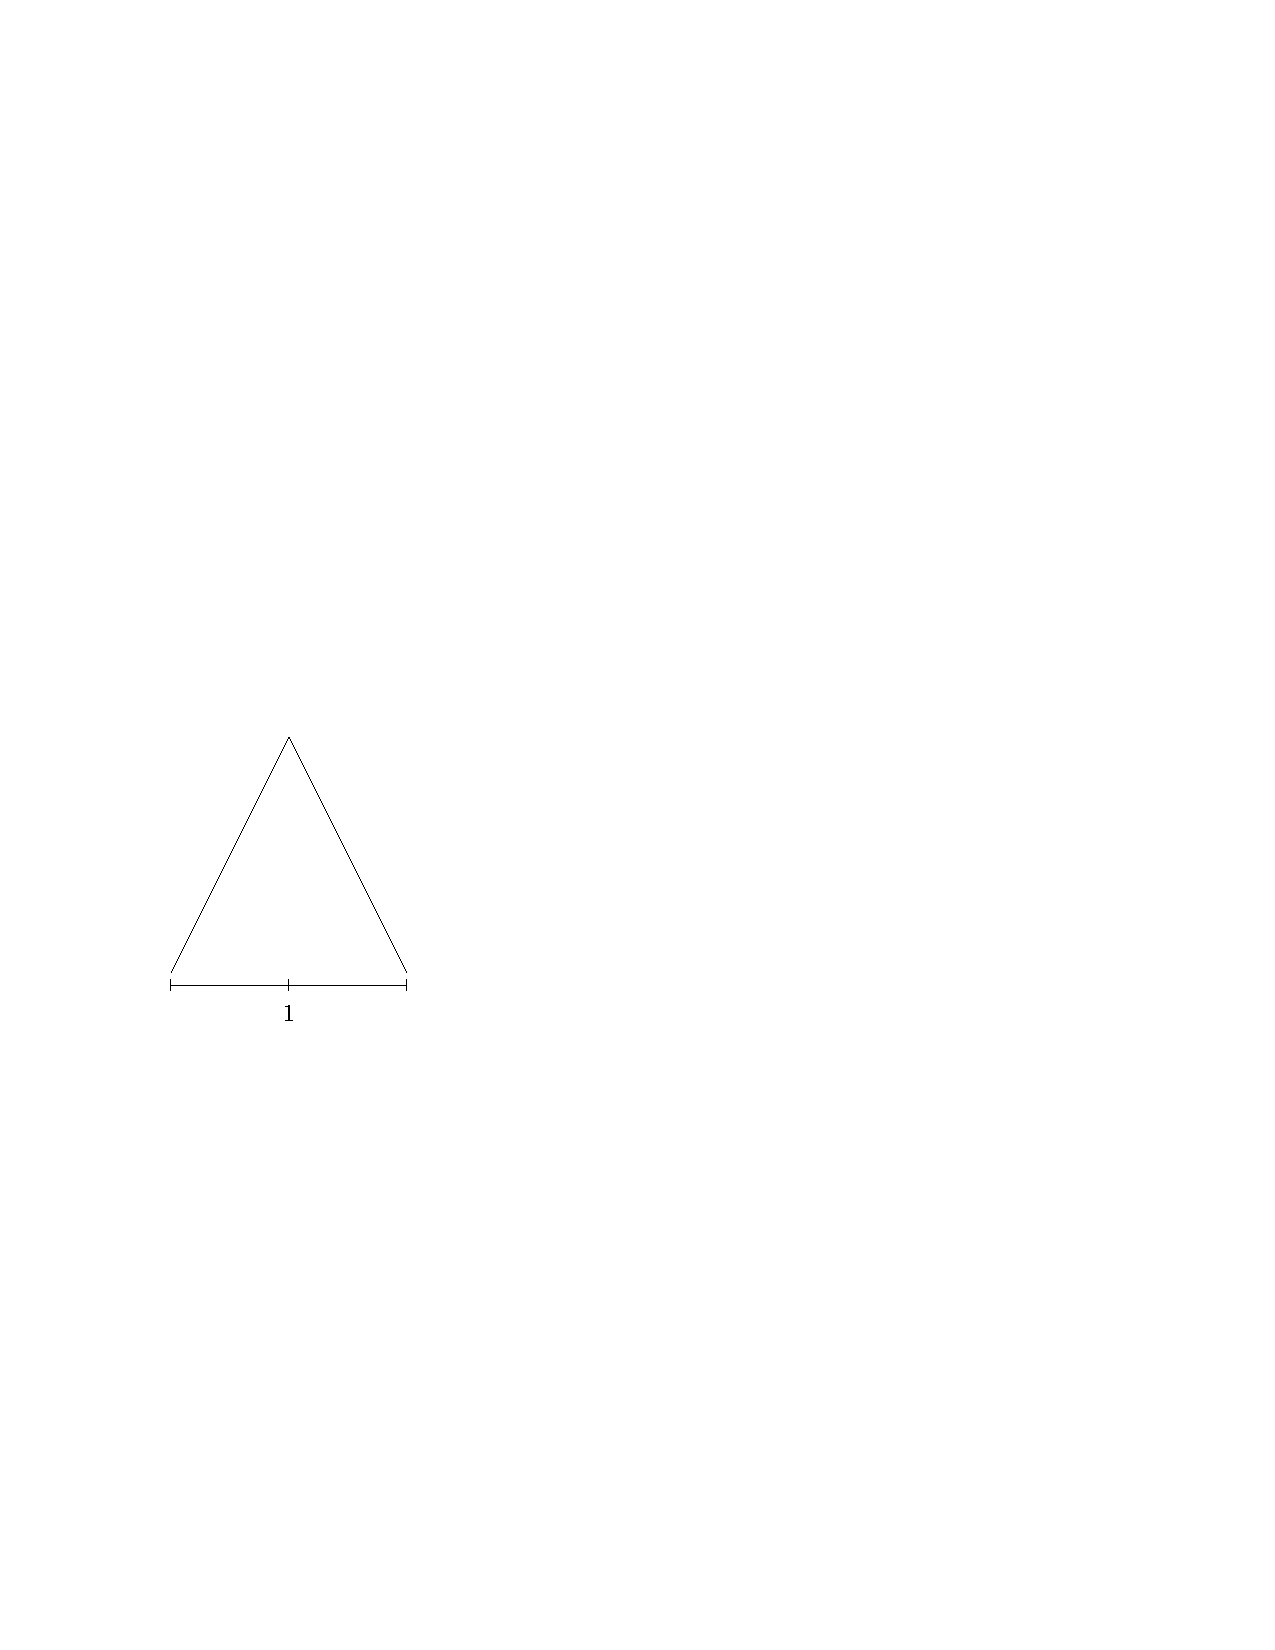
\includegraphics[width=4cm]{1dbasis1.pdf}\qquad
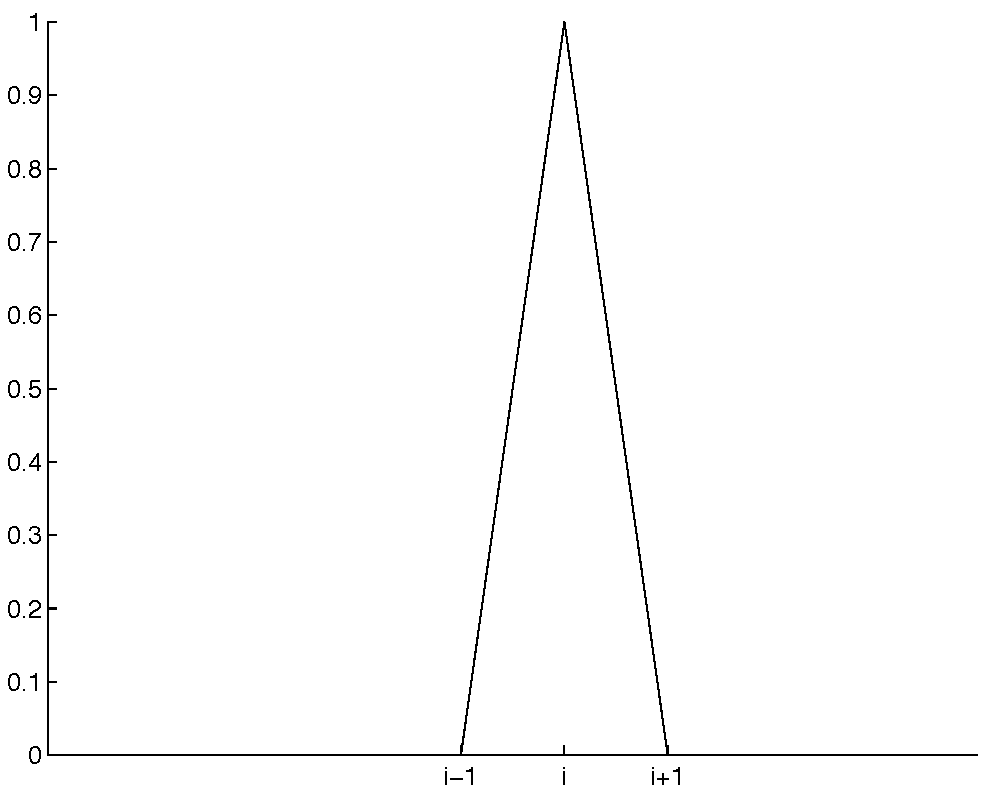
\includegraphics[width=5cm]{basisfunction.pdf}
\caption{Diagram of $\varphi(x)$ (left) and $\varphi_{\ell,i}(x)$ (right).}
\end{figure} 


Let us recall the finite element interpolation in Section \ref{linearFE} as
\begin{equation}\label{key}
u(x) \approx u_\ell(x) := \sum_{ 0\le i \le 2^\ell} u(x_{\ell,i}) \varphi_{\ell,i}(x),
\end{equation}
for any smooth function $u(x)$ on $(0,1)$. The above interpolation will converge as $\ell \to \infty$, which shows that
\begin{equation}\label{key}
{\rm span} \left\{  \varphi(w_\ell x + b_{\ell,i}) \right\} \quad \text{is dense in} \quad H^1(0,1).
\end{equation}
Thus, we may have the next concise relation:
\begin{equation}\label{key}
\begin{split}
\text{FE space} =  &{\rm span} \left\{  \varphi(w_\ell x + b_{\ell,i}) ~|~ 0\le i \le 2^\ell, \ell = 1, 2, \cdots \right\} 
\\
\subset  &{\rm span} \left\{  \varphi(w x + b) ~|~  w, b \in \mathbb{R} \right\}.
\end{split}
\end{equation}
In other words, the finite element space can be understood as the linear combination of $\varphi(w x + b)$ with certain special choice of $w$ and $b$. 

Here, we need to point out that this ${\rm span} \left\{  \varphi(w x + b) ~|~  w, b \in \mathbb{R} \right\}$ is exact the deep neural networks with one hidden layer (shallow neural networks) with activation function $\varphi(x)$. More precisely, 
\begin{equation}\label{key}
f \in {\rm span} \left\{  \varphi(w x + b) ~|~  w, b \in \mathbb{R} \right\},
\end{equation}
means there exist positive integer $N$ and $w_j, b_j \in \mathbb{R}$ such that 
\begin{equation}\label{key}
f = \sum_{j=1}^N a_j \varphi(w_j x + b_j),
\end{equation}
which is also called one hidden neural network function with $N$ neurons.

\begin{remark}
	\begin{enumerate}
		\item By making $w_\ell$ and $b_{\ell,i}$ in \eqref{def_g} arbitrary, we get a much larger class of 
		function which is exact a special neural network with activation function $\varphi(x)$.
		\item Generalizations: 
		\begin{enumerate}
			\item activation function $\varphi$ can be different, such as ${\rm ReLU}(x) = \max\{0,x\}$.
			\item There is a natural extension for high dimension $d$ as
			\begin{equation}\label{key}
			\left\{  \varphi(w\cdot x + b) \right \},
			\end{equation}
			where $w\in \mathbb{R}^d$, $b\in \mathbb{R}$ and $\displaystyle w\cdot x = \sum_{i=1}^d w_i x_i$.
			This is called ``deep'' neural network with one hidden layer.
		\end{enumerate}
	\end{enumerate}
\end{remark}


%\input{3FEM/2dFEM}

%%\section{Basic Artificial Neural Network}
Artificial neural networks (ANNs) are biologically inspired computer programs designed to simulate the way in which the human brain processes information.
%This model is just a model for a class of parameterized function with some special function structure which can be presented simply using some simple network graph. This method is began from the approximation of neural network in human.
\subsection{basic element: Nonlinear active function with affine map}
Mc Culloch-Pitts Neuron, also known as M-P Neuron, is the earliest neural network that was discovered in 1943. In this model, the neurons are connected by connection weights, and the activation function is used in binary. The threshold is used to determine whether the neuron will fire or not.

M-P element(approximation of one neuron): this is a very simple example for interpolating a function $f: \mathbb{R}^m \to \mathbb{R}$, with the next definition:
\begin{equation}\label{eq:M-P}
f_{M-P}(x) = \sigma( w \cdot x + b)
\end{equation}
with $w  \in \mathbb{R}^{m} $ and $\sigma$ is called active function which can be chosen like:
\begin{equation}
\sigma (x) = \frac{1}{1 + e^{-x}},
\end{equation}
or
\begin{equation}
\sigma(x) = tanh(x) = \frac{e^x - e^{-x}}{e^x + e^{-x}}.
\end{equation}
Basically, both these two functions are smooth and have two horizontal asymptotic lines, which can be seen as a smoothing approximation for
\begin{equation}
H(x) =
\begin{cases}
1  &\text{if}  ~x < 0, \\
0 &\text{if}~ x \le 0.
\end{cases}
\end{equation}
But now, the most commonly used activation function is the so-called ``Rectified Linear Unit'' (ReLU), which is defined by
\begin{equation}
{\rm ReLU}(x) = \max\{0,x\}.
\end{equation}
%We will talk about some basic stuff about variant of activation function in the next chapter and 
It is also very important in the approximation theory for such as one hidden layer ANN networks.
This is often shown as the next picture:
\begin{figure}[!ht]
	\center{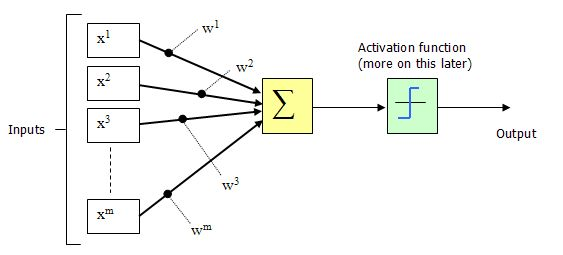
\includegraphics[width=10cm] {M-P.jpeg}}
	\caption{M-P neuron.}
\end{figure}

\subsection{neural network}
Now we want to use this simple basic element to construct some more complex model(from one neuron to neural network). A bionic but simple construction is to increase the basic element in both horizontal and vertical direction, which means the network would be like the one in Fig~\ref{fig:ANN}.
\begin{figure}[!ht]
	\center{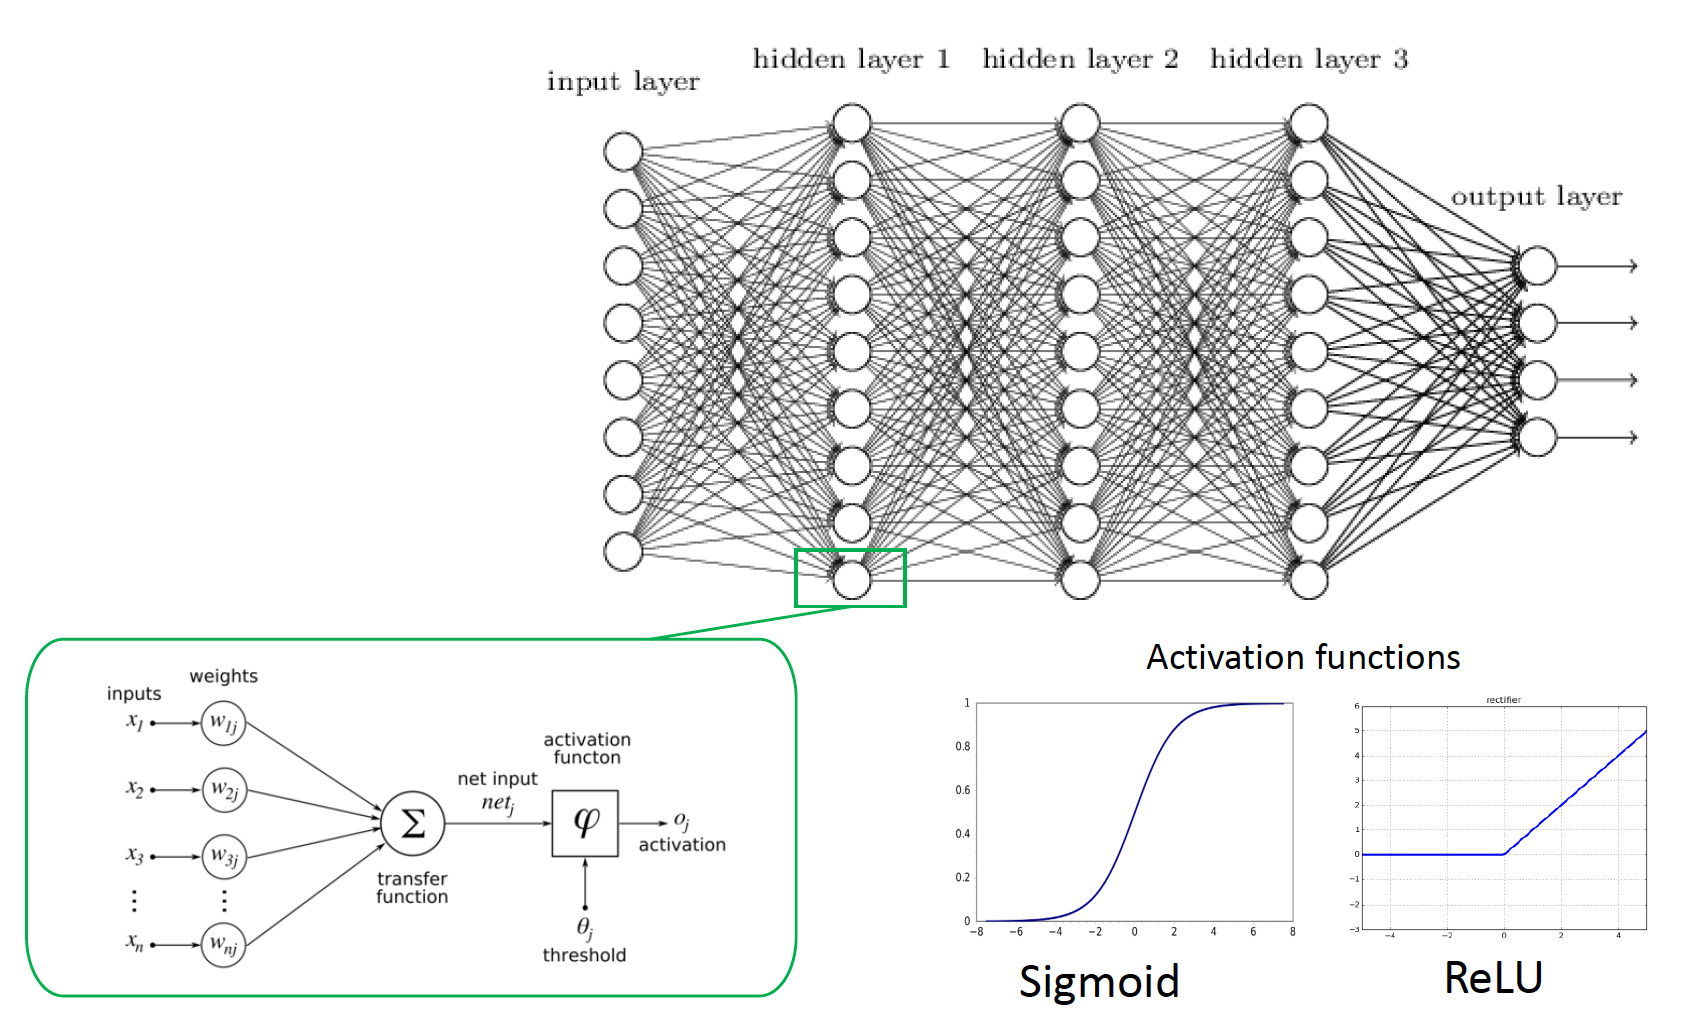
\includegraphics[width=12cm,height=6cm] {ANN.png}}
	\caption{ANN}
	\label{fig:ANN}
\end{figure}

This is called fully connected feedforward neural network. Now we want to give a more compressive expression, we collect all the output in $k$-th level $[f^{k}]_l$, $l = 1,\cdots, n_k$.
So we can have the output in $k+1$-th level under this setting with
\begin{equation}
{f}^{k+1} = \theta^{k+1}\circ \sigma (f^{k})
\end{equation}
with
\begin{equation}
\theta^k(x) = w^kx+b \in\mathbb{R}^{n_{k+1}},
\end{equation} 
where 
\begin{equation}
w^k= 
\begin{pmatrix}
w_1 \\
\vdots \\
w_{n_{k+1}}
\end{pmatrix},\qquad \mbox{ with }\qquad w_i \in \mathbb{R}^{n_k}.
\end{equation} 

So, we get the final iterative definition with the last output and initial input of this network like:
\begin{equation}
\begin{cases}
f^{0} &= \theta^0(x), \\
f^{\ell} &= \theta^{\ell}\circ \sigma(f^{\ell-1}), \quad \ell = 1:J, \\
f(x;\Theta) &= f^J.
\end{cases}
\end{equation}
Here we note 
\begin{equation}
\Theta = \{ (\theta^0, \cdots, \theta^J) \}.
\end{equation}

%\subsection{Interpolation by optimization}
%So the  interpolation process can be seen as a optimization problem in the special function class if the activation function for every elements and  the network structure parameter $\mathcal{N}_K$ are given:
%\begin{equation}
%\mathcal{F} = \{\bm{f}_K(W_K;\bm{x}) ~|~  \bm{f}_0 = (\bm{x}^{T},1)^{T}\},
%\end{equation}
%and the optimization problem can be seen as
%\begin{equation}
%%\mathop{\min}_{f \in \mathcal{F}}  \frac{1}{N}\sum_{i=1}^N \|f(X^i) - Y^i\|^2 =
%\mathop{\min}_{W_K \in T_3(\mathcal{N}_K)}  L(W_K) := \frac{1}{N}\sum_{i=1}^N \|\bm{f}_K(W_K; X^i) - Y^i\|^2.
%\end{equation}
%But $\mathcal{F}$ this is neither a linear space nor a convex set.

%\iffalse
\subsection{Back-Propagation}
Here we will talk about how to compute $\nabla_{\Theta} f(x;\Theta)$ by using chain rule which is called Back-Propagation (BP) algorithm in deep learning. 
Thus we have
\begin{equation}
\frac{\partial {f}(x; \Theta)}{ \partial w^k} = \frac{\partial {f}^J}{\partial {f}^{J-1}} \cdot \frac{ \partial {f}^{J-1}}{\partial {f}^{J-2}} \cdots \frac{ \partial {f}^k}{\partial w^k}.
\end{equation}
We can see from the above that, we only need to compute those terms like:
\begin{equation}
\frac{ \partial {f}^k}{\partial w^{k}}  \quad \text{and} \quad \frac{\partial {f}^k}{\partial {f}^{k-1}}  \quad k = 1,2,\cdots,J.
\end{equation}
We have
\begin{equation}\label{eq:partial-f}
\frac{\partial {f}^k}{\partial {f}^{k-1}} =
w^k{\rm Diag}(\sigma'(f^{k-1})) ,
\end{equation}
and
\begin{equation}
\frac{ \partial {f}^k}{\partial w^{k}}  = \delta \otimes \sigma(f^{k-1}).
\end{equation}


In short, BP algorithm can be expressed as:
\begin{algorithm}[H]
	\begin{algorithmic}[1]
		\State {\bf{Input:}}  $X^i$ and $W_K$;
		\For{$k = K:-1:1$}
		\State Compute and save
		$$\frac{ \partial {f}^k}{\partial w^{k}}  \quad \text{and} \quad \frac{\partial {f}^k}{\partial {f}^{k-1}}$$.
		\State Compute
		$$\frac{ \partial {f}^J}{\partial w^{k}} = \frac{\partial {f}^J}{\partial {f}^{J-1}} \cdot \frac{ \partial {f}^{J-1}}{\partial {f}^{J-2}} \cdots \frac{ \partial {f}^k}{\partial w^{k}}$$ 
		\EndFor
	\end{algorithmic}
	\caption{Back-Propagation Algorithm}
\end{algorithm}




%\subsection{Classical DNN}
First, we have a more comprehensive notation for classical DNN models.
\begin{equation}\label{eq:DNNdef_J}
\begin{aligned}
{\rm{DNN}_J} :=\{& f:f=
\theta^J \circ \sigma \circ \theta^{J-1} \cdots \sigma \circ \theta^0(x), \\
&\theta^\ell \in \mathbb{R}^{n^{\ell+1} \times (n^\ell+1)}, \quad n^0 = d, \quad n^{J+1} = 1, \quad n^\ell \in \mathbb{N}^+\}.
\end{aligned}
\end{equation}

Thus to say, we have the general two definition for DNN with
\begin{itemize}
\item  $\sigma \circ \theta$ type:
\begin{equation}\label{eq:sigma+theta}
\begin{aligned}
f^0 &= x, \\
f^{i+1} &= \sigma \circ \theta^{i}(f^i), \\
{\rm DNN}_J &= \{\theta^J(f^J)\}.
\end{aligned}
\end{equation}

\item $\theta \circ \sigma $ type:
\begin{equation}\label{eq:theta+sigma}
\begin{aligned}
f^0 &= \theta^0(x), \\
f^{i+1} &=  \theta^{i+1} \circ \sigma (f^i), \\
{\rm DNN}_J &= \{f^J\}.
\end{aligned}
\end{equation}
\end{itemize}

\subsection{DNN type ResNet}
For simplicity, we choose $\sigma \circ \theta$ type as example.

\paragraph{ResNet}
The ResNet can be written as
\begin{equation}\label{ori-ResNet-dnn}
\begin{cases}
f^0 &= x, \\
f^{i} &= \sigma \left( P^i f^{i-1} + \mathcal{F}^{ i} (f^{i-1}) \right), \quad i = 1:J ,\\
{\rm ResNet}_{J} &= \{  \theta^J f^{J} \}.
\end{cases}
\end{equation}
Here
\begin{equation}\label{eq:F-ResNet}
\mathcal{F}^{i} (f^{i-1}) = \xi^{i} \circ \sigma \circ \eta^{i} (f^{i-1}),
\end{equation}
means ResNet with skip connection distant 2. And $P^i$ is use to fit the dimension as
\begin{equation}\label{eq:P^i}
P^i: \mathbb{R}^{n_{i-1}} \mapsto \mathbb{R}^{n_i}.
\end{equation}

\paragraph{iResNet} 
The iResNet can be written as:
\begin{equation}\label{ori-iResNet-dnn}
\begin{cases}
f^0 &= x, \\
f^{i} &=  P^i f^{i-1} + \mathcal{F}^{ i} (f^{i-1}) , \quad i = 1:J ,\\
{\rm iResNet}_{J} &= \{  \theta^J f^{J} \}.
\end{cases}
\end{equation}
Here
\begin{equation}\label{eq:F-iResNet}
\mathcal{F}^{i} (f^{i-1}) = \xi^{i} \circ \sigma \circ \eta^{i}  \circ \sigma (f^{i-1}),
\end{equation}
means iResNet with skip connection distant 2. 
And $P^i$ is use to fit the dimension as in ResNet in \eqref{eq:P^i}.

The only difference between ResNet and iResNet can be viewed as 
putting a $\sigma$ in different places. 

And we also need to notice that ${\rm ResNet}_J$ or  ${\rm iResNet}_J$
are often called DNN with $2J$-th layers if the distance of skip connection
is $2$ as in \eqref{eq:F-ResNet} and \eqref{eq:F-iResNet}.

\subsection{DNN type MgNet}
Similar with ResNet, we can rewrite MgNet.

Here use $\theta \circ \sigma$ type as example.
\begin{equation}\label{ori-MgNetNet-dnn}
\begin{cases}
f^0 &= 0, \quad f^0 = \theta^0(x) \\
f^{i} &=  P^i f^{i-1} + \mathcal{F}^{ i} (f^{i-1}) , \quad i = 1:J ,\\
{\rm iResNet}_{J} &= \{  f^{J} \}.
\end{cases}
\end{equation}
Here
\begin{equation}\label{eq:F-MgNet}
\mathcal{F}^{i} (f^{i-1}) = \xi^{i} \left( f^{i-1} +  \sigma \circ \eta^{i} \circ \sigma(f^{i-1}) \right).
\end{equation}

\subsection{DNN type DenseNet}
In fact, DenseNet might be simple for definition in DNN case. 

Here use $\sigma \circ \theta$ type as example.
\begin{equation}\label{ori-DenseNet-dnn}
\begin{cases}
f^0 &= x, \\
f^{i} &=   \sigma \circ \theta^{i}([f^{i-1}, f^{i-2}, \cdots, f^0]) , \quad i = 1:J ,\\
{\rm DenseNet}_{J} &= \{  \theta^J f^{J} \}.
\end{cases}
\end{equation}

Here $[f^{i-1}, f^{i-2}, \cdots, f^0]$ means a long vector by collecting all 
outputs from $f^0$ to $f^{i-1}$, thus to say
$$
{\rm dim}([f^{i-1}, f^{i-2}, \cdots, f^0]) = \sum_{i=0}^{i-1} n_i.
$$


\section{A Universal DNN Model}

\subsection{Kailai's definition}
A DNN is defined as a tuple $M=(\mathcal{S}, \mathcal{O}, s_0, F, \delta)$
\begin{itemize}
	\item $\mathcal{S}$ is a non-empty set of states.
	\item $\mathcal{O}$ is a finite, non-empty set of parametrized operators.
	\item $s_0\in \mathcal{S}$ is the initial input. 
	\item $F\subset \mathcal{S}$ is the set of final states~(outputs). 
	\item $\delta: 2^{\mathcal{S}}\times \mathcal{O} \rightarrow \mathcal{S}$ is the mapping function. 
\end{itemize}
and an acceptable ordered sequence $(\delta_1, \delta_2, \ldots, \delta_n)$, which maps $s_0$ to $\delta_n \circ \delta_{n-1} \circ \delta_1 (s_0) \in F$.

\subsection{Juncai's definition}
The idea is that, deep neural network comes from the composition of linear and 
element-wise activation. 
So, we define the basic component of our model as:
\begin{equation}
\mathcal L_{\sigma,1}(x) = Wx + b + \sigma(\tilde Wx + \tilde b),
\end{equation}
where 
\begin{equation}
x \in \mathbb{R}^d, \quad W, ~ \tilde W \in \mathbb{R}^{n \times d} \quad \text{and} \quad b,~ \tilde b \in \mathbb{R}^n.
\end{equation}
Then we try to define an important operator in the universal DNN model,
known as $\mathcal L_{\sigma, \ell}(x^1, \cdots, x^k)$, by recursion of $\mathcal L_{\sigma,1}$. 
For $x^i \in \mathbb{R}^{n_i}, i = 1:\ell$,  we have
\begin{equation}
\mathcal L_{\sigma, \ell}(x^1, \cdots, x^k) = \mathcal L_{\sigma,1}
\left([\mathcal L_{\sigma, \ell-1}(\hat x^1), \mathcal L_{\sigma, \ell-1}(\hat x^2), \cdots, \mathcal L_{\sigma, \ell-1}(\hat x^k)]\right),
\end{equation}
where
\begin{equation}
\mathcal L_{\sigma, \ell-1}(\hat x^k) = \mathcal L_{\sigma, \ell-1} (x^1, \cdots, x^{k-1}, x^{k+1}, \cdots, x^\ell),
\end{equation}
and 
\begin{equation}
[\mathcal L_{\sigma, \ell-1}(\hat x^1), \mathcal L_{\sigma, \ell-1}(\hat x^2), \cdots, \mathcal L_{\sigma, \ell-1}(\hat x^k)],
\end{equation}
means to collect all the output of $\mathcal L_{\sigma, \ell-1}(\hat x^k)$ into one vector such 
that it can be the input of $\mathcal L_{\sigma, 1}$.

Then we define the $J-$layer universal DNN model by recursion as:
\begin{equation}
\begin{cases}
f^{0} &= x,  \\
f^{\ell} &= \mathcal L_{\sigma, \ell}(f^0,\cdots, f^{\ell-1}), \quad \ell = 1:J, \\
f(x) &= W^J f^J + b^J. 
\end{cases}
\end{equation}




  
%\chapter{Approximation Properties of Neural Network Function
%Class}\label{ch:approx}
%\input{6DL/DNN-FEM}
%
\section{Weierstrass Theorem}  
To approximate any continuous function, a very simple idea is to approximate the function in a polynomial space. 
An important property of this space is that polynomials can approximate any reasonable function!
\begin{itemize}
\item $P_n(\mathbb{R}^d)$ is dense in $C(\Omega)$ [Weierstrass theorem]
\item $P_n(\mathbb{R}^d)$ is dense in all Sobolev spaces: $L^2(\Omega), W^{m,p}(\Omega), \ldots$
\end{itemize}

\begin{theorem}
Let $\Omega\subset R^n$ be a  closed and bounded set. Given any continuous function $f(x)$ on $\Omega$, there exists a sequence of polynomials $\{p_n(x)\}$ such 
that 
\begin{equation}
\displaystyle \lim_{n\rightarrow \infty} \max_{x\in \Omega}|f(x)-p_n(x)|=0
\end{equation}
\end{theorem}
\begin{proof}
Let us first give the proof for $d=1$ and $\Omega=[0,1]$. Given $f:[0,1]\rightarrow R$ be a  continuous function. 

Let
\begin{equation}
\tilde f(x)=f(x)-l(x)
\end{equation}
where $l(x)=f(0)+x(f(1)-f(0))$.
Then $\tilde f(0)=\tilde f(1)=0$. Noting that $l(x)$ is a linear function, hence without lose of generality, we can only consider the 
case $f:[0,1]\rightarrow R$ with $f(0)=f(1)=0$. 
Since $f$ is continuous on the closed interval $[0,1]$, then $f$ is uniformly continuous on $[0,1]$.

First we extend $f$ to be zero outside of $[0,1]$ and obtain $f: R\rightarrow R$, then it is obviously that $f$ is still uniformly continuous. 

Next for $0\le x\le 1$, we construct
\begin{equation}
p_n(x)=\int_{-1}^1f(x+t)Q_n(t)dt=\int_{-x}^{1-x}f(x+t)Q_n(t)dt=\int_{0}^{1}f(t)Q_n(t-x)dt
\end{equation} 
where $Q_n(x)=c_n(1-x^2)^n$ and 
\begin{equation}\label{intq}
\int_{-1}^1 Q_n(x) dx=1.
\end{equation} 
Thus $\{p_n(x)\}$ is a sequence of polynomials. 

Since 
\begin{align}
\int_{-1}^1 (1-x^2)^n dx&=2\int_{0}^1 (1-x^2)^n dx=  2\int_{0}^1 (1-x)^n(1+x)^n dx\\ 
&\ge 2\int_{0}^1 (1-x)^n dx=\frac{2}{n+1}> \frac{1}{n}.
\end{align}
Combing with $\int_{-1}^1 Q_n(x) dx=1$, we obtain $c_n< n$ implying that for any $\delta>0$
 \begin{equation}\label{qest}
 0\le Q_n(x)\le n(1-\delta^2)^n \quad (\delta\le |x|\le 1),
 \end{equation}
so that $Q_n\rightarrow 0$ uniformly in $\delta\le |x|\le 1$ as $n\rightarrow \infty$. 

Given any $\epsilon >0$, since $f$ in uniformly continuous, there exists $\delta>0$ such that for any $|y-x|<\delta$, we have 
\begin{equation}\label{fcont}
|f(y)-f(x)|< \frac{\epsilon}{2}.
\end{equation}
Finally, let $M=\max |f(x)|$, using \eqref{fcont}, \eqref{intq} and \eqref{qest}, we have 
\begin{align}
\big| p_n(x)-f(x)\big|&=\big|\int_{-1}^1(f(x+t)-f(t))Q_n(t)dt\big|\le \int_{-1}^1 \big| f(x+t)-f(t)\big| Q_n(t)dt\\
&\le 2M \int_{-1}^{-\delta} Q_n(t)dt+ \frac{\epsilon}{2}\int_{-\delta}^{\delta} Q_n(t)dt+ 2M\int_{\delta}^1 Q_n(t)dt\\
&\le 4M n(1-\delta^2)^n + \frac{\epsilon}{2}< \epsilon
\end{align}
for all large enough $n$, which proves the theorem. 

The above proof generalize the high dimensional case easily.   We
consider the case that
$$
\Omega=[0,1]^d.
$$
By extension and using cut off function,  W.L.O.G.  that we assume
that $f=0$ on the boundary of $\Omega$ and we then extending this
function to be zero outside of $\Omega$.  

Let us consider the special polynomial functions
\begin{equation}
  \label{Qn}
Q_n(x)=c_n\prod_{k=1}^d(1-x_k^2)  
\end{equation}
Similar proof can then be applied. 
\end{proof}























 
\subsection{Curse of dimensionality}
Number of coefficients for polynomial space $P_n(\mathbb{R}^d)$  is
$$
	N = \binom{d+n}{n} = \frac{(n+d)!}{d!n!}.
$$
For example $n = 100$:
		\begin{table}
			\centering
			\begin{tabular}{|c|c|c|c|}
				\hline
				$d = $&  $2$ &  $4$ & $8$\\
				\hline
				$N=$  & $5\times10^3$ & $4.6\times10^6$  & $3.5\times10^{11}$ 	\\
				\hline
			\end{tabular}
		\end{table}
As the this table shows, the dimension of the polynomial space $P_n(\mathbb{R}^d)$   increases rapidly as the degree $n$ increases. This leads to an extremely large space therefore very expensive to approximate functions in polynomial spaces in high dimensions.
\subsection{Runge's phenomenon}
A natural way to approximate a given function on any interval $[a,b]$ is to use an $n$-degree polynomial $p_n(x)$ by $n+1$ equispaced  points, namely
$$
x_i=a+{b-a\over n},\quad i=0,1,2,\cdots,n.
$$
By Weierstrass' theorem, we expect a more accurate reconstruction of $f(x)$ by using more points. But this is not always true as shown in the following example. 
%Consider the case where one desires to interpolate through $n+1$ equispaced points of a function $f(x)$ using the n-degree polynomial $p_n(x)$ that passes through those points. Naturally, one might expect from Weierstrass' theorem that using more points would lead to a more accurate reconstruction of $f(x)$. However, this particular set of polynomial functions $p_n(x)$ is not guaranteed to have the property of uniform convergence; the theorem only states that a set of polynomial functions exists, without providing a general method of finding one.

Consider the Runge function (a scaled version of the Witch of Agnesi)
$$ 
f(x)=\frac{1}{1+25x^{2}}.
$$
Runge found that if this function is interpolated at equidistant points $x_i$ between $-1$ and $1$ such that:
$$
x_{i}={\frac{2i}{n}}-1,\quad i\in \left\{0,1,\dots ,n\right\}
$$
with a polynomial $p_n(x)$ of degree $\leq n$, the resulting interpolation oscillates toward the ends of the interval, i.e. close to $-1$ and $1$. It can even be proven that the interpolation error increases (without bound) when the degree of the polynomial is increased:

$$\lim_{{n\rightarrow \infty }}\left(\max_{{-1\leq x\leq 1}}|f(x)-p_{n}(x)|\right)=+\infty.$$
This shows that high-degree polynomial interpolation at equidistant points can be troublesome.

\begin{figure}
	\begin{center}
		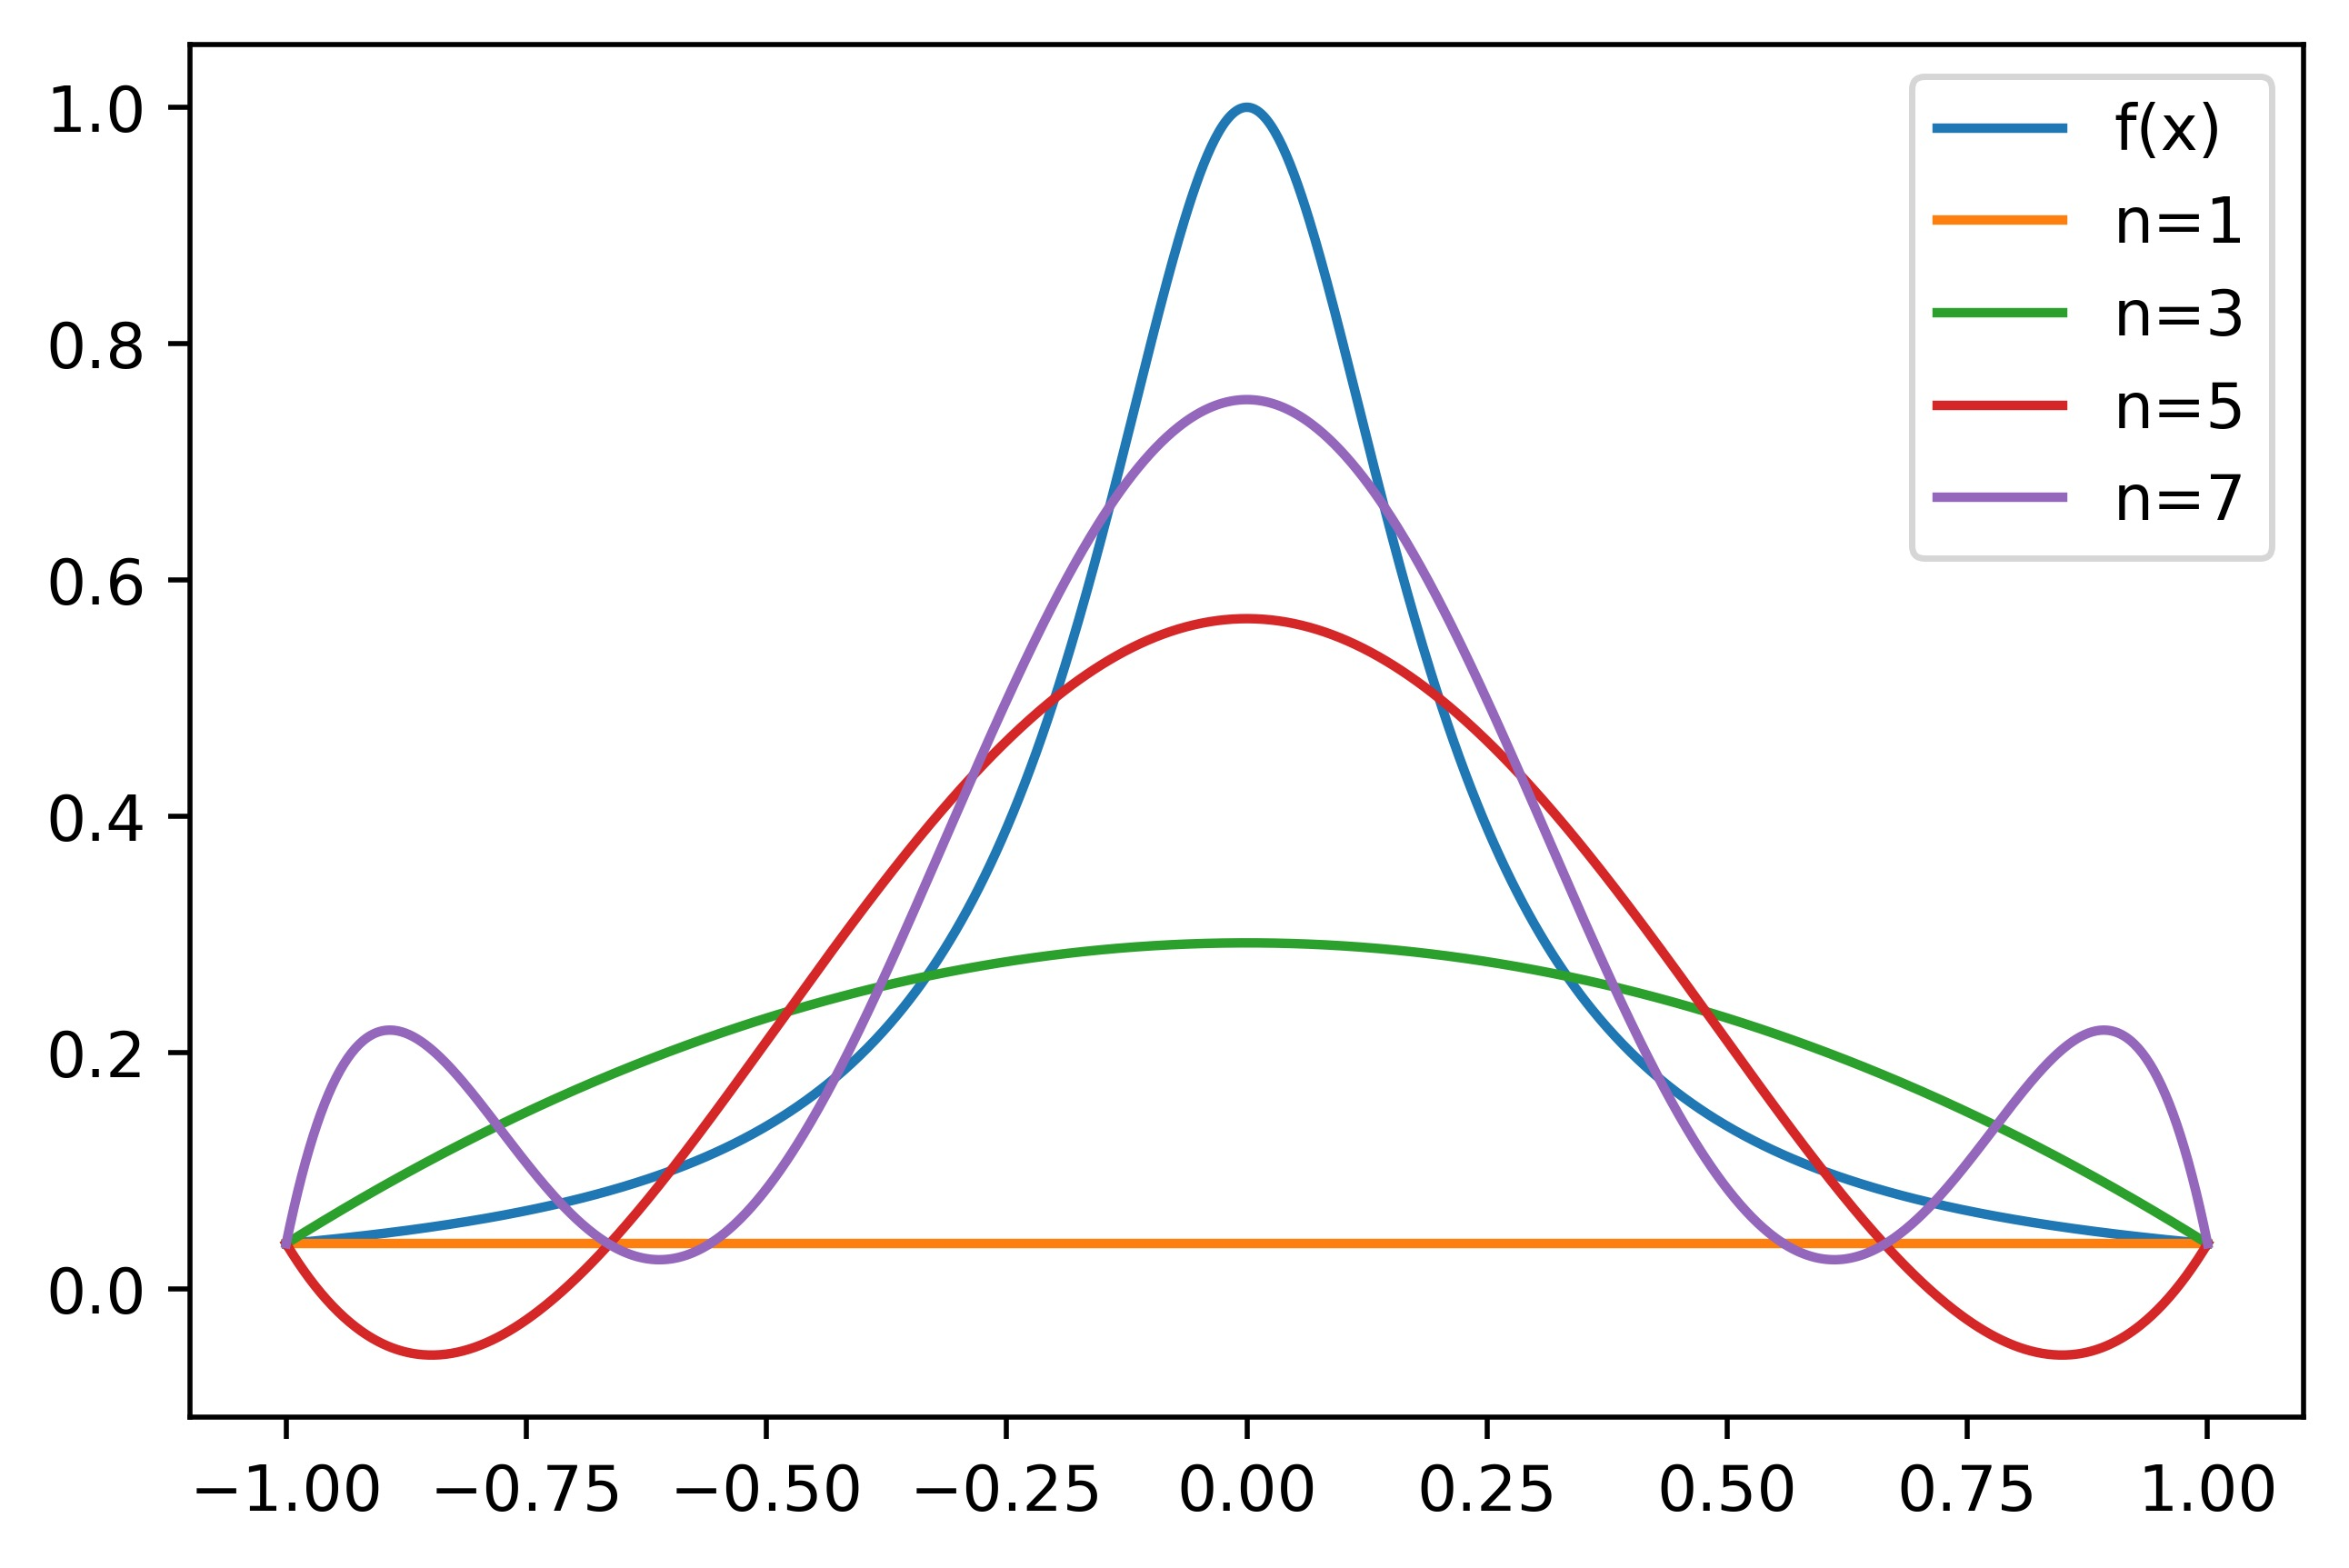
\includegraphics[scale=0.1]{6DL/pic/Runge.jpeg}
		\caption{Runge's phenomenon: Runge function $f(x)=\frac{1}{1+25x^{2}}$ and its polynomial interpolation $p_n(x)$.}
	\end{center}
\end{figure}

The experiment shows that  the polynomials $p_n(x)$ produced in this manner may in fact diverge away from $f(x)$ as $n$ increases. This typically occurs in an oscillating pattern that magnifies near the ends of the interpolation points. This phenomenon is attributed to Runge.

Thus, this particular set of polynomial functions $p_n(x)$ is not guaranteed to have the property of uniform convergence. In other words, Weierstrass' theorem guarantees the existence of the polynomial functions, but how to find such polynomials is not provided.

\section{Fourier transform and Fourier series}
We make use of the theory of tempered distributions (see
\cite{strichartz2003guide} for an introduction)
and we begin by collecting some results of independent interest, which
will also be important later. 
\subsection{Fourier transform}
Before studying the Fourier transform, we first consider Schwartz space which is defined below.
\begin{definition} \label{def:schwarz}
The Schwartz space $\mathcal{S}\left(\mathbb{R}^{n}\right)$ is the topological vector space of functions $f: \mathbb{R}^{n} \rightarrow \mathbb{C}$ such that $f \in C^{\infty}\left(\mathbb{R}^{n}\right)$ and
$$
x^{\alpha} \partial^{\beta} f(x) \rightarrow 0 \quad \text { as }|x| \rightarrow \infty
$$
for every pair of multi-indices $\alpha, \beta \in \mathbb{N}_{0}^{n} .$ For $\alpha, \beta \in \mathbb{N}_{0}^{n}$ and $f \in \mathcal{S}\left(\mathbb{R}^{n}\right)$ let
(5.10)
$$
\|f\|_{\alpha, \beta}=\sup _{\mathbb{R}^{n}}\left|x^{\alpha} \partial^{\beta} f\right|
$$
A sequence of functions $\left\{f_{k}: k \in \mathbb{N}\right\}$ converges to a function $f$ in $\mathcal{S}\left(\mathbb{R}^{n}\right)$ if
$$
\left\|f_{n}-f\right\|_{\alpha, \beta} \rightarrow 0 \quad \text { as } k \rightarrow \infty
$$
for every $\alpha, \beta \in \mathbb{N}_{0}^{n}$.
\end{definition}
The Schwartz space consists of smooth functions whose derivatives and the function itself decay at infinity faster than any power. Schwartz functions are rapidly decreasing. When there is no ambiguity, we will write $\mathcal{S}\left(\mathbb{R}^{n}\right)$ as $\mathcal{S}$.
Roughly speaking, tempered distributions grow no faster than a polynomial at infinity.

\begin{definition}
A tempered distribution $T$ on $\mathbb{R}^{n}$ is a continuous linear functional $T: \mathcal{S}\left(\mathbb{R}^{n}\right) \rightarrow \mathbb{C} .$ The topological vector space of tempered distributions is denoted by $\mathcal{S}^{\prime}\left(\mathbb{R}^{n}\right)$ or $\mathcal{S}^{\prime} .$ If $\langle T, f\rangle$ denotes the value of $T \in \mathcal{S}^{\prime}$ acting on $f \in \mathcal{S}$
then a sequence $\left\{T_{k}\right\}$ converges to $T$ in $\mathcal{S}^{\prime}$, written $T_{k} \rightarrow T$, if
$$
\left\langle T_{k}, f\right\rangle \rightarrow\langle T, f\rangle
$$
for every $f \in \mathcal{S}$.
\end{definition}
Since $\mathcal{D} \subset \mathcal{S}$ is densely and continuously imbedded, we have $\mathcal{S}^{\prime} \subset \mathcal{D}^{\prime} .$ Moreover, a distribution $T \in \mathcal{D}^{\prime}$ extends uniquely to a tempered distribution $T \in \mathcal{S}^{\prime}$ if and only if it is continuous on $\mathcal{D}$ with respect to the topology on $\mathcal{S}$. Every function $f \in L_{\text {loc }}^{1}$ defines a regular distribution $T_{f} \in \mathcal{D}^{\prime}$ by
$$
\left\langle T_{f}, \phi\right\rangle=\int f \phi d x \quad \text { for all } \phi \in \mathcal{D}.
$$
If $|f| \leq p$ is bounded by some polynomial $p,$ then $T_{f}$ extends to a tempered distribution $T_{f} \in \mathcal{S}^{\prime}$, but this is not the case for functions $f$ that grow too rapidly at infinity.

The Schwartz space is a natural one to use for the Fourier transform. Differentiation and multiplication exchange roles under the Fourier transform and therefore so do the properties of smoothness and rapid decrease. As a result, the Fourier transform is an automorphism of the Schwartz space. By duality, the Fourier transform is also an automorphism of the space of tempered distributions.

\begin{definition}\label{def:fourier1}
The Fourier transform of a function $f \in \mathcal{S}\left(\mathbb{R}^{n}\right)$ is the function $\hat{f}: \mathbb{R}^{n} \rightarrow \mathbb{C}$ defined by 
$$
\hat{f}(\omega)= \int f(x) e^{-2 \pi i\omega \cdot x} d x.
$$
The inverse Fourier transform of $f$ is the function $\check{f}: \mathbb{R}^{n} \rightarrow \mathbb{C}$ defined by
$$
\check{f}(x)=\int f(\omega) e^{2 \pi i\omega \cdot x} d k.
$$
\end{definition}

\begin{definition}\label{def:fourier2}
The Fourier transform of a tempered distribution $f \in \mathcal{S}'$ is  defined by 
$$
\langle \hat{f}, \phi\rangle = \langle f, \hat \phi\rangle,\quad \forall \phi\in \mathcal{S}.
$$ 
\end{definition}

The support of a continuous function $f$ is the closure  of the set $\{x\in \mathbb{R}: f(x)\neq 0\}$.
\begin{properties}
The Fourier transform has the following properties
\begin{enumerate}
\item If $f\in \mathcal{S}'$ and the support of $\hat f$ is $\{0\}$, then $f$ is a polynomial.
\item If $f\in \mathcal{S}'$ and the support of $\hat f$ is a single point $\{a\}$, then $f(x)=e^{2\pi iax}P(x)$, where $P(x)$ is a polynomial.
\end{enumerate}
\end{properties}







\subsection{Poisson summation formula}
% Qingguo put the Poisson summation formula here in this file:  statement and sketch of proof

\begin{theorem}
Let $f \in L^{1}(\mathbb{R})$ and $f$ is continuous. Then we have for almost all $(x, \omega ) \in \mathbb{R} \times \hat{\mathbb{R}}$ that
$$
T \sum_{n \in \mathbb{Z}} f(x+n T) e^{-2 \pi i \omega (x+n T)}=\sum_{n \in \mathbb{Z}} \hat{f}\left(\omega +\frac{n}{T}\right) e^{2 \pi i n x / T}
$$
where both sides converge absolutely.

In addition,  let $\Lambda$ be the lattice in $\mathbb{R}^{d}$ consisting of points with integer coordinates. 
For a function $f$ in $L^{1}\left(\mathbb{R}^{d}\right)$ and $f$ is continuous, we have 
$$
\sum_{\omega  \in \Lambda} f(x+\omega )=\sum_{\nu \in \Lambda} \hat{f}(\omega ) e^{2 \pi i x \cdot \omega }.
$$
where both series converge absolutely and uniformly on $\Lambda$. 
\end{theorem} 

\begin{proof}
We just give a proof of a simple case that $f: \mathbb{R} \rightarrow \mathbb{C}$ is a Schwarz function (see Definition \ref{def:schwarz}).
Let:
$$
F(x)=\sum_{n \in \mathbb{Z}} f(x+n).
$$
Then $F(x)$ is 1-periodic (because of absolute convergence), and has Fourier coefficients:
$$
\begin{aligned}
\hat{F}_{\omega } &=\int_{0}^{1} \sum_{n \in \mathbb{Z}} f(x+n) e^{-2 \pi i \omega x} \mathrm{~d} x \\
&=\sum_{n \in \mathbb{Z}} \int_{0}^{1} f(x+n) e^{-2 \pi i \omega  x} \mathrm{~d} x \quad \text { because } f \text { is Schwarz, so convergence is uniform}\\
&=\sum_{n \in \mathbb{Z}} \int_{n}^{n+1} f(x) e^{-2 \pi i\omega  x} \mathrm{~d} x \\
&=\int_{\mathbb{R}} f(x) e^{-2 \pi i \omega  x} \mathrm{~d} x\\
&=\hat{f}(k)\\
\end{aligned}
$$
 where $\hat{f}$ is the Fourier transform of $f$.
 

Therefore by the definition of the Fourier series of $f:$
$$
F(x) =\sum_{\omega  \in \mathbb{Z}} \hat{f}(k) e^{2\pi i \omega x}.
$$
Choosing $x=0$ in this formula:
$$
\sum_{n \in \mathbb{Z}} f(n)=\sum_{\omega  \in \mathbb{Z}} \hat{f}(\omega )
$$
as required.
\end{proof}






\subsection{A special cut-off function}
Let us first state the following simple result that can be obtained by following a calculation given in Section 3 of \cite{johnson2015saddle}. 
\begin{lemma} Given $\alpha>1$, consider
 \begin{equation}\label{alpha-g}
  g(t) = \begin{cases} 
      e^{-(1-t^2)^{1 - \alpha}} & t\in (-1,1) \\
      0 & \text{otherwise}.
   \end{cases}
 \end{equation}
then there is a constant $c_\alpha$ such that
 \begin{equation}\label{eq_181}
  |\hat{g}(\omega )|\lesssim e^{-c_\alpha|\omega |^{1-\alpha^{-1}}},
 \end{equation}
\end{lemma}
\begin{proof}
Consider the asymptotic behavior of the Fourier transform
$$
F(\omega )=\int_{-\infty}^{\infty} g(t) e^{2\pi i \omega  t} dt=2 \operatorname{Re} \int_{0}^{1} e^{2\pi i \omega  t- (1-t^{2})^{1-\alpha}} dt
$$
for $|\operatorname{Re} \omega | \gg 1.$ (Without loss of generality, we can restrict ourselves to real $\omega  \geq 0$).  
With a change of variable $x=1-t$,
$$
F(\omega )=2 \operatorname{Re} \int_{0}^{1} e^{f(x)} dx
$$
with 
$
f(x)=2\pi i \omega  - 2\pi i \omega   x- (2x-x^2)^{1-\alpha}\approx \tilde f(x)+O\left(x^{2-\alpha}\right)
$
and 
$$
\tilde f(x) = 2\pi i \omega  - 2\pi i \omega    x - (2 x)^{1-\alpha}.
$$
The saddle point is the $x=x_0$ where $f'(x_0)=0$. Since
$
\tilde f'(x)=-2\pi i \omega  + (\alpha-1)2^{1-\alpha} x^{-\alpha},
$
$$
x_{0} \approx \tilde x_0=\left (2^{-\alpha} (\alpha-1) / i \omega \pi \right )^{1 / \alpha} \sim \omega ^{-1 / \alpha}.
$$
Therefore $\tilde f(\tilde x_{0}) \sim \omega ^{(\alpha-1) / \alpha}$ asymptotically. The second derivative is 
$$
\tilde f'' (\tilde x_{0} )=-2^{1-\alpha}  \alpha(\alpha-1) \tilde x_{0}^{-\alpha-1}=-i^{(\alpha+1) / \alpha} 2 A \omega ^{(\alpha+1)/\alpha},
$$
where
$$
A=2\alpha  (\alpha-1)^{-1/\alpha}\pi^{(\alpha+1)/\alpha}.
$$
Now,
\begin{equation}
\begin{split}
\tilde f(x)\approx &\tilde f(\tilde x_0) + {\tilde f''(\tilde x_0)\over 2} (x-\tilde x_0)^2
\\
=&2\pi i \omega  - (\alpha - 1)^{1\over \alpha}(i\omega \pi )^{\alpha -1\over \alpha}  - (\alpha - 1)^{1-\alpha\over \alpha} (i\omega \pi )^{\alpha -1\over \alpha}
\\
&-i^{(\alpha+1) / \alpha} A \omega ^{(\alpha+1)/\alpha}(x- 2^{-1}(\alpha - 1)^{-{1\over \alpha}}(i\omega \pi )^{-{1\over \alpha}} )^2.
\end{split}
\end{equation} 
Choose a contour $x=i^{-1 / \alpha}u$, in which case  
$$
\tilde f(x) \approx \tilde f(\tilde x_{0}) -i^{(\alpha-1) / \alpha} A \omega ^{(\alpha+1) / \alpha}\left(u-u_{0}\right)^{2},
$$
which is a path of descent so we can perform a Gaussian integral. 

Recall that the integral of 
\begin{equation}\label{gaussInt}
\int_{-\infty}^{\infty} e^{-a u^{2}} d u=\sqrt{\pi / a}
\end{equation}
as long as Re$a>0,$ which is true here. Note also that, in the limit as $\omega $ becomes large, the integrand becomes zero except close to $u=\sqrt{1 / 2 \omega },$ so we can neglect the rest of the contour and treat the integral over $u$ as going from $-\infty$ to $\infty$. (Thankfully, the width of the Gaussian $\Delta u \sim \omega ^{-3 / 4}$ goes to zero faster than the location of the maximum $u_{0} \sim \omega ^{-1 / 2},$ so we don't have to worry about the $u=0$ origin). Also note that the change of variables from $x$ to $u$ gives us the Jacobian factor for 
$$dx=i^{-1 / \alpha}d u.$$ 
Thus, when all is said and done, we obtain the exact asymptotic form of the Fourier integral for $\omega  \gg 1$: 
\begin{equation}
\begin{split}
F(\omega ) \approx &2 \operatorname{Re}\int_{0}^{1} e^{\tilde f(\tilde x_0) - i^{(\alpha-1) / \alpha} A \omega ^{(\alpha+1) / \alpha}\left(u-u_{0}\right)^{2}} dx
\\
=&2 \operatorname{Re} e^{\tilde f(\tilde x_0)} i^{-1 / \alpha} \int_{-\infty}^{\infty} e^{- i^{(\alpha-1) \over  \alpha} A \omega ^{(\alpha+1) / \alpha}\left(u-u_{0}\right)^{2}} du
\\
=&2 \operatorname{Re} e^{\tilde f(\tilde x_0)} \pi^{1/2}i^{-1 / \alpha}  i^{(1-\alpha) \over  2\alpha} A^{-1/2} \omega ^{-(\alpha+1) / 2\alpha}\qquad \text{ by \eqref{gaussInt}} 
\\
=&2 \operatorname{Re}\left[\sqrt{\frac{\pi}{(i \omega )^{(\alpha+1) / \alpha} A}} e^{\tilde f(\tilde x_0)}\right]
\\
\approx &2 \operatorname{Re}\left[\sqrt{\frac{\pi}{(i \omega )^{(\alpha+1) / \alpha} A}} e^{ 2\pi i \omega - 2\pi i \omega  \tilde x_{0}- \left[\left(2-\tilde x_{0}\right) \tilde x_{0}\right]^{1-\alpha}}\right]
\end{split}
\end{equation}  
with $x_{0}$ and $A$ given above.  Notice that $ \tilde x_0\sim \omega ^{-1 / \alpha}$. Thus,
$$
|F(\omega ) | \approx  e^{-c_\alpha|\omega |^{1-\alpha^{-1}}}.
$$
\end{proof}

\subsection{Fourier transform of polynomials}
We begin by noting that an activation
function $\sigma$, which satisfies a polynomial growth condition
$|\sigma(x)| \leq C(1 + |x|)^n$ for some constants $C$ and $n$, is a
tempered distribution. As a result, we make this assumption on our
activation functions in the following theorems. We briefly note that
this condition is sufficient, but not necessary (for instance an
integrable function need not satisfy a pointwise polynomial growth
bound) for $\sigma$ to be represent a tempered distribution.

 We begin by studying the convolution of $\sigma$ with a Gaussian mollifier. Let $\eta$ be a Gaussian mollifier
 \begin{equation}
  \eta(x) = \frac{1}{\sqrt{\pi}}e^{-x^2}.
 \end{equation}
Set $\eta_\epsilon=\frac{1}{\epsilon}\eta(\frac{x}{\epsilon})$. Then consider 
\begin{equation}
\label{sigma-epsilon}
\sigma_{\epsilon}(x):=\sigma\ast{\eta_\epsilon}(x)=\int_{\mathbb{R}}\sigma(x-y){\eta_\epsilon}(y)dy
\end{equation}
for a given activation function $\sigma$.
It is clear that $\sigma_{\epsilon}\in C^\infty(\mathbb{R})$. Moreover, by considering the Fourier transform (as a tempered
distribution) we see that
\begin{equation}\label{eq_278}
 \hat{\sigma}_{\epsilon} = \hat{\sigma}\hat{\eta}_{\epsilon} = \hat{\sigma}\eta_{\epsilon^{-1}}.
\end{equation} 


We begin by stating a lemma which characterizes the set of polynomials in terms of their
 Fourier transform.
\begin{lemma}\label{polynomial_lemma} Given a tempered distribution
  $\sigma$,  the following statements are equivalent:
\begin{enumerate}
\item $\sigma$ is a polynomial 
\item $\sigma_\epsilon$ given by \eqref{sigma-epsilon} is a polynomial for any
  $\epsilon>0$. 
\item $\text{\normalfont supp}(\hat{\sigma})\subset \{0\}$. 
\end{enumerate}
\end{lemma}
\begin{proof}
  We begin by proving that (3) and (1) are equivalent.  This follows
  from a characterization of distributions supported at a single point
  (see \cite{strichartz2003guide}, section 6.3). In particular, a
  distribution supported at $0$ must be a finite linear combination of
  Dirac masses and their derivatives.  In particular, if
  $\hat{\sigma}$ is supported at $0$, then
  \begin{equation}
   \hat{\sigma} = \displaystyle\sum_{i=1}^n a_i\delta^{(i)}.
  \end{equation}
  Taking the inverse Fourier transform and noting that the inverse
  Fourier transform of $\delta^{(i)}$ is $c_ix^i$, we see that
  $\sigma$ is a polynomial. This shows that (3) implies (1), for the
  converse we simply take the Fourier transform of a polynomial and
  note that it is a finite linear combination of Dirac masses and
  their derivatives.
  
  Finally, we prove the equivalence of (2) and (3). For this it
  suffices to show that $\hat{\sigma}$ is supported at $0$ iff
  $\hat{\sigma}_\epsilon$ is supported at $0$. This follows from
  equation \ref{eq_278} and the fact that $\eta_{\epsilon^{-1}}$ is
  nowhere vanishing.
\end{proof}

As an application of Lemma \ref{polynomial_lemma}, we give a
simple proof of the result in the next section.   


\end{document}

 
